\documentclass[11pt, twoside, fleqn]{article} % use \documentstyle for old LaTeX compilers

\usepackage[ngerman]{babel} % 'french', 'german', 'spanish', 'danish', etc.
\usepackage{float}
\everymath{\displaystyle}
\usepackage{amsmath,nccmath} 
\usepackage{anyfontsize}

% Helvetica = Arial for sections
\usepackage{helvet}
\fontfamily{Name_OF_Font_Family}\selectfont

\usepackage{titlesec}
\titleformat{\section}
  {\fontfamily{phv}\selectfont\Large\bfseries}
  {\thesection}{1em}{}

\usepackage{titlesec}
\titleformat{\subsection}
  {\fontfamily{phv}\selectfont\large\bfseries}
  {\thesubsection}{1em}{}
  
\usepackage{titlesec}
\titleformat{\subsubsection}
  {\fontfamily{phv}\selectfont\bfseries}
  {\thesubsubsection}{1em}{}

\usepackage{amsfonts} 
\usepackage{amssymb}
\usepackage{mathtools}
\usepackage{hyperref}
\usepackage{txfonts}
\usepackage{mathdots}
\usepackage[classicReIm]{kpfonts}
\usepackage[utf8]{inputenc}
\usepackage{graphicx}
\usepackage{biblatex} 
\usepackage{csquotes}
\usepackage{geometry}
\usepackage{siunitx}
\usepackage{subcaption}
\usepackage[export]{adjustbox}
\usepackage{wrapfig}
\usepackage[justification=centering]{caption}


\setlength\mathindent{0pt}
\input{insbox}

% set row height 
\usepackage{stackengine}
\newcommand\xrowht[2][0]{\addstackgap[.5\dimexpr#2\relax]{\vphantom{#1}}}

%\usepackage[scaled=.90]{helvet}% Helvetica, served as a model for arial
\usepackage{titlesec}
 \geometry{
 a4paper,
 total={175mm,257mm},
 left=20mm,
 top=20mm,
 }

% caption set
\usepackage{caption} 
\captionsetup[table]{justification=raggedright,singlelinecheck = false}
\DeclareCaptionFormat{myformat}{\fontfamily{phv}\selectfont#1#2#3\par}
\captionsetup{format=myformat,font=small}

% table set
\usepackage{xcolor,fancyhdr}
\usepackage{array,multirow,colortbl}
\usepackage{multicol}
 
% set fancy header, remove foot number page
\usepackage{fancyhdr}
\pagestyle{fancy}
\fancyhead[LE,RO]{\small\thepage}
\fancyhead[RE]{\small \emph{\nouppercase{\leftmark}}}
\fancyhead[LO]{\small \emph{\nouppercase{\rightmark}}}
\setlength{\headheight}{14pt}
\cfoot{} 

\newcolumntype{C}[1]{>{\centering\arraybackslash }b{#1}}

% Numbering automatically for sections 
\numberwithin{equation}{section}
\numberwithin{table}{section}
\usepackage[tablename=Tabelle]{caption}
\numberwithin{figure}{section}
\usepackage[figurename=Bild]{caption}

% Matlab listing
\usepackage[numbered,framed]{matlab-prettifier}
\usepackage{filecontents}
\let\ph\mlplaceholder % shorter macro
\lstMakeShortInline"

\lstset{
  style              = Matlab-editor,
  basicstyle         = \mlttfamily,
  escapechar         = ",
  mlshowsectionrules = true,
    literate=%
    {Ö}{{\"O}}1
    {Ä}{{\"A}}1
    {Ü}{{\"U}}1
    {ß}{{\ss}}2
    {ü}{{\"u}}1
    {ä}{{\"a}}1
    {ö}{{\"o}}1
}

% Change Inhalt's word
\renewcommand*\contentsname{Inhalt}

\begin{document}
\thispagestyle{empty} % remove the header
\begin{figure}[H]
  \centerline{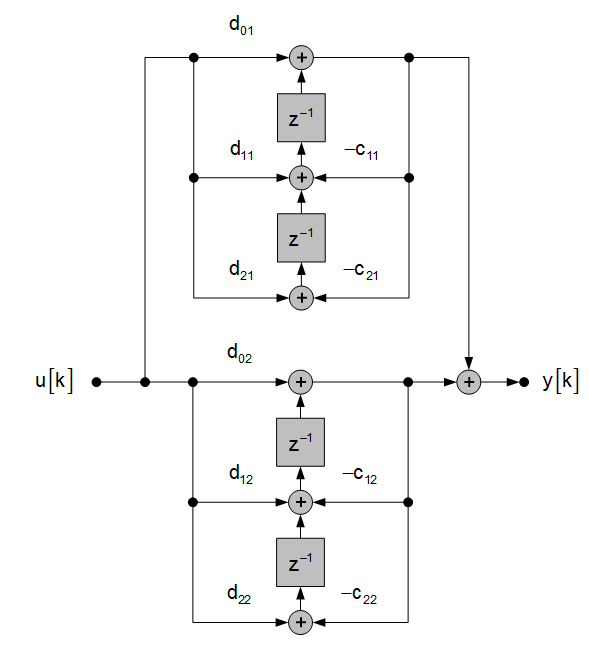
\includegraphics[width=0.6\textwidth]{SignalflussParallelstruktur.png}}
\end{figure}

\noindent \bigskip

\centerline  {\fontfamily{phv}\fontsize{50}{60}\selectfont Systemtheorie Teil B} 

\noindent \medskip

\centerline  {\fontfamily{phv}\fontsize{23}{30}\selectfont  - Zeitdiskrete Signale und Systeme -}

\noindent \bigskip
\noindent \bigskip

\centerline  {\fontfamily{phv}\fontsize{23}{30}\selectfont  Manfred Strohrmann}\medskip

\noindent 

\centerline  {\fontfamily{phv}\fontsize{23}{30}\selectfont Urban Brunner}

\vspace{6.0\baselineskip}

\begin{figure}[H]
  \centerline{
\includegraphics[width=0.6\textwidth]{FH_Logo.png}}
\end{figure}

\clearpage
\newpage

\thispagestyle{empty}
\section*{Änderungsindex}
\begin{table}[H]
\setlength{\arrayrulewidth}{.1em}
\setlength{\fboxsep}{0pt}
\begin{tabular}{wl{1.4cm} | wl{2.3cm} | wl{2.5cm} | wl{9.8cm}}
\xrowht{15pt}

\fontfamily{phv}\selectfont\textbf{Version} &
\fontfamily{phv}\selectfont\textbf{Datum} & 
\fontfamily{phv}\selectfont\textbf{Verfasser} & 
\fontfamily{phv}\selectfont\textbf{Änderungen}\\ \hline \xrowht{15pt}

\multirow{2}{*}{\fontfamily{phv}\selectfont{10}} &
\multirow{2}{*}{\fontfamily{phv}\selectfont{15.08.2020}} &
\fontfamily{phv}\selectfont{M. Strohrmann,} &
\fontfamily{phv}\selectfont{Fehlerkorrektur, Ausgabe für Vorlesung}\\ \xrowht{10pt}

&
&
\fontfamily{phv}\selectfont{U. Brunner} &
\fontfamily{phv}\selectfont{WS 2020/21}\\ \hline \xrowht{15pt}

\multirow{2}{*}{\fontfamily{phv}\selectfont{9}} &
\multirow{2}{*}{\fontfamily{phv}\selectfont{15.09.2015}} &
\fontfamily{phv}\selectfont{M. Strohrmann,} &
\fontfamily{phv}\selectfont{Fehlerkorrektur, Ausgabe für Vorlesung}\\ \xrowht{10pt}

&
&
\fontfamily{phv}\selectfont{U. Brunner} &
\fontfamily{phv}\selectfont{WS 2017/18}\\ \hline \xrowht{15pt}

\multirow{2}{*}{\fontfamily{phv}\selectfont{8}} &
\multirow{2}{*}{\fontfamily{phv}\selectfont{15.09.2015}} &
\fontfamily{phv}\selectfont{M. Strohrmann,} &
\fontfamily{phv}\selectfont{Fehlerkorrektur, Ausgabe für Vorlesung}\\ \xrowht{10pt}

&
&
\fontfamily{phv}\selectfont{U. Brunner} &
\fontfamily{phv}\selectfont{WS 2015/16}\\ \hline \xrowht{8pt}

\multirow{3}{*}{\fontfamily{phv}\selectfont{7}} &
\multirow{3}{*}{\fontfamily{phv}\selectfont{15.03.2015}} &
\multirow{2}{*}{\fontfamily{phv}\selectfont{M. Strohrmann,}} &
\fontfamily{phv}\selectfont{Trennung von Text, Übungsaufgaben und Musterlösungen,}\\ \xrowht{8pt}

&
&
\multirow{2}{*}{\fontfamily{phv}\selectfont{U. Brunner}} &
\fontfamily{phv}\selectfont{Überarbeitung Kapitel 11: Diskrete Fourier Transformation,}\\ \xrowht{8pt}

&
&
&
\fontfamily{phv}\selectfont{Ausgabe für Vorlesung SS 2015}\\ \hline \xrowht{15pt}

\multirow{2}{*}{\fontfamily{phv}\selectfont{6}} &
\multirow{2}{*}{\fontfamily{phv}\selectfont{15.03.2014}} &
\fontfamily{phv}\selectfont{M. Strohrmann,} &
\fontfamily{phv}\selectfont{Integration der Systemtheorie Online Funktionen,}\\ \xrowht{10pt}

&
&
\fontfamily{phv}\selectfont{U. Brunner} &
\fontfamily{phv}\selectfont{Korrektur von Fehlern und Überarbeitung}\\ \hline \xrowht{15pt}

\fontfamily{phv}\selectfont{5} &
\fontfamily{phv}\selectfont{14.03.2012} &
\fontfamily{phv}\selectfont{M. Strohrmann} &
\fontfamily{phv}\selectfont{Korrektur von Fehlern und Überarbeitung}\\ \hline \xrowht{15pt}

\multirow{2}{*}{\fontfamily{phv}\selectfont{4}} &
\multirow{2}{*}{\fontfamily{phv}\selectfont{14.03.2014}} &
\multirow{2}{*}{\fontfamily{phv}\selectfont{M. Strohrmann}} &
\fontfamily{phv}\selectfont{Kapitel 10: Strukturen digitaler Systeme}\\ \xrowht{10pt}

&
&
&
\fontfamily{phv}\selectfont{Korrektur von Fehlern und Überarbeitung}\\ \hline \xrowht{15pt}

\fontfamily{phv}\selectfont{3} &
\fontfamily{phv}\selectfont{14.03.2011} &
\fontfamily{phv}\selectfont{M. Strohrmann} &
\fontfamily{phv}\selectfont{Korrektur von Fehlern und Überarbeitung}\\ \hline \xrowht{15pt}

\fontfamily{phv}\selectfont{2} &
\fontfamily{phv}\selectfont{01.10.2010} &
\fontfamily{phv}\selectfont{M. Strohrmann} &
\fontfamily{phv}\selectfont{Einarbeiten von Musterlösungen und Vertiefung}\\ \hline \xrowht{15pt}

\fontfamily{phv}\selectfont{1} &
\fontfamily{phv}\selectfont{01.04.2010} &
\fontfamily{phv}\selectfont{M. Strohrmann} &
\fontfamily{phv}\selectfont{Erstausgabe}\\  

\end{tabular}\bigskip
\end{table}

\newpage
\pagenumbering{Roman}
\thispagestyle{empty}
%\pagenumbering{gobble} %Page numbering empty
\tableofcontents

\newpage

\thispagestyle{empty} % empty
\mbox{}

\pagenumbering{arabic}

\section{Einleitung}
Steigende Anforderungen an die Produktqualität und immer kürzer werdende Entwicklungszei-ten erfordern stetige Verbesserungen im Produktentstehungsprozess. Eine Schlüsselrolle kommt dabei der Systembeschreibung und der Systemsimulation zu. Systemsimulationen lassen sich erheblich schneller und reproduzierbarer umsetzen als der Aufbau von Musterteilen. Aus diesem Grund steigt in der Produktentwicklung der Anteil von Simulationsaufgaben an. Ingenieure be-nötigen damit ein interdisziplinäres Systemverständnis, mit dem komplexe Systeme erfasst, be-schrieben und simuliert werden können.\newline
Unter einem System wird die Abstraktion eines Prozesses oder Gebildes verstanden, das mehrere Signale zueinander in Verbindung setzt. Systeme sind dabei oft interdisziplinär, sie erstrecken sich über mehrere Fachrichtungen. Einige dieser Systeme lassen sich direkt mit algebraischen Gleichungen \newline beschreiben. Ein Beispiel für ein solches System ist ein Spannungsteiler, bei dem sich Ausgangsspannung direkt aus der Eingangsspannung und dem Widerstandsverhältnis ergibt. Oftmals finden bei praktischen Anwendungen aber Einschwingvorgänge statt. Sie ergeben sich aus Energiespeichern, deren Zustand sich durch eine Anregung zeitabhängig ändert. Ein Beispiel für ein System mit Energiespeicher ist ein Kondensator, der über einen Widerstand aufgeladen wird. Die Ausgangsspannung des Kondensators ist zeitabhängig. Systeme mit Energiespeichern werden als dynamische Systeme bezeichnet. Andere bekannte Beispiele für dynamische Syste-me sind Pendelbewegungen, das Verhalten elektrischer Schaltungen mit Kondensatoren und Spulen sowie thermische und chemische Prozesse. Es wird sich zeigen, dass die Systembe-schreibung bei dynamischen Systemen aus einer oder mehreren Differentialgleichungen besteht.\newline
Die Systemtheorie liefert eine Theorie zur einheitlichen Beschreibung von dynamischen Syste-men, die sehr unterschiedlicher Natur sein können. Insbesondere für regelungstechnische An-wendungen ist die Systemtheorie damit eine wesentliche Voraussetzung, da sie Systeme in einer einheitlichen Weise beschreibt. Weitere Anwendungen in der Ingenieurwissenschaft sind die Automatisierungstechnik, Nachrichtentechnik, Messtechnik, Verfahrenstechnik, Informatik so-wie die klassische Elektrotechnik. In aller Regel werden abstrakte Systembeschreibungen mit Verzicht auf das Detail eingesetzt. Teilweise werden die Systembeschreibungen durch detaillierte Modelle kritischer Teilsysteme ergänzt. Durch die abstrakte Beschreibungsform bleibt der Über-blick über das System erhalten. 

\clearpage

\subsection{Strukturierung des Buchs }

In der Systemtheorie werden Systeme und ihre Wirkung auf Signale beschrieben. Deshalb wer-den in Kapitel 2 zunächst wesentliche Beschreibungsformen für Signale im Zeitbereich wieder-holt. Es werden sogenannte Sprung- und Impulsfunktionen definiert, die bevorzugte Testsignale dynamischer Systeme sind. Das Einschwingverhalten wird in vielen Fällen durch abklingende harmonische Schwingungen beschrieben, die als komplexe Exponentialfunktionen beschrieben werden.\newline
Einführende Beispiele in Kapitel 3 zeigen, dass viele zeitkontinuierliche Systeme über Differentialgleichungen beschrieben werden. Eine besondere Stellung nehmen dabei lineare, zeitinvarian-te Systeme ein. Ihre Systemreaktion lässt sich im Zeitbereich auf verschiedene Arten bestimmen. Neben der direkten Lösung der Differentialgleichung wird die Berechnung der Systemantwort über das Superpositionsprinzip und Faltungsintegral bestimmt. Die Zweiteilung von Signalen und Systemen zieht sich weiter durch das Buch. \newline
Zur Lösung von Differentialgleichungen wird in Kapitel 4 die Laplace-Transformation einge-führt. Nach der Diskussion der Laplace-Transformation für Signale werden in Kapitel 5 Differentialgleichungen mithilfe der Laplace-Transformation gelöst, und es wird der Begriff der Über-tragungsfunktion zeitkontinuierlicher Systeme eingeführt. An der Übertragungsfunktion können wichtige Systemeigenschaften direkt abgelesen werden, ohne die Systemantwort ausrechnen zu müssen. Die Interpretation der Übertragungsfunktion wird beschrieben und an Beispielen ange-wendet. In der Elektrotechnik kommt der Beschreibung von RLC-Schaltkreisen eine besondere Bedeutung kommt zu. Sie wird als eine Anwendung der Laplace-Transformation ausführlich diskutiert.\newline
Die Fourier-Reihe beschreibt periodische Signale näherungsweise mit einer Grundschwingung und ihren Oberschwingungen. Mit ihr wird in Kapitel 6 der Begriff des Spektrums eingeführt. Es wird darüber hinaus gezeigt, wie mithilfe der Fourier-Transformation nichtperiodische Signale im Frequenzbereich beschrieben werden können. Dabei werden die Parallelen zwischen Fourier-Reihe und Fourier-Transformation sowie Laplace- und Fourier-Transformation herausgearbeitet. Anschließend wird in Kapitel 7 die Fourier-Transformation zur Interpretation von Systemen im Frequenzbereich herangezogen. \newline
Durch den Einsatz von Filtern werden in der Elektrotechnik erwünschte Spektralanteile von unerwünschten Spektralanteilen getrennt. Die Grundlagen zum Entwurf und zur Realisierung von Filterschaltungen werden in Kapitel 8 erarbeitet. Dabei wird allgemein auf die Zielsetzung der Filterentwicklung eingegangen, und es werden spezielle Filterentwurfsverfahren vorgestellt. Au-ßerdem werden aktive und passive Schaltungen für die Realisierung unterschiedlicher Filterent-würfe angegeben.\newline
Die lineare Systemtheorie ermöglicht die Systembeschreibung durch Strukturschaubilder, die aus vernetzten Übertragungsgliedern bestehen. Die dabei verwendeten Übertragungsglieder werden insbesondere in der Regelungstechnik eingesetzt. Wesentliche Übertragungsglieder werden in Kapitel 9 vorgestellt und ihr Zeit- und Frequenzverhalten zusammengefasst. \newline
In der modernen Regelungstechnik werden Systeme im sogenannten Zustandsraum beschrieben. Dabei ist jeder Koordinate des Zustandsraums eine Zustandsgröße zugeordnet, die den Zustand eines Energiespeichers des Systems beschreibt. Die Eingangs- und Ausgangssignale sowie die Zustandsgrößen sind Funktionen der Zeit. Diese Darstellung kommt damit der praktischen Vor-stellung näher als ihre Darstellung im Laplace- oder Fourier-Bereich. Die Darstellung von Syste-men im Zustandsraum wird in Kapitel 10 eingeführt.\newline
Kapitel 11 beschreibt einen Leitfaden zur Modellbildung von Systemen. Es wird aufgezeigt, wie mit dem gewonnenen Wissen auch komplexere Systeme über mathematische Gleichungen be-schrieben werden können. Parameter der Gleichungen werden mit Methoden der Parameteriden-tifikation bestimmt. Das Vorgehen wird an einem praktischen Beispiel illustriert.\newline
In der Elektrotechnik steigt der Trend, analoge Größen durch geeignete Sensoren zu erfassen und dann digital weiterzuverarbeiten. Teil B dieser Buchreihe widmet sich daher zeitdiskreten Signalen und Prozessen.\newline 
In der Praxis gibt es Signale, die nicht durch analytische Funktionen beschrieben werden kön-nen. Teil C behandelt deshalb stochastische Signale und Prozesse. Es wird auf die statistischen Grundlagen sowie ihr Einsatz in der Signalverarbeitung eingegangen. \newline
In diesem Buch werden wesentliche Zusammenhänge an Ende jeden Abschnittes in Tabellenform zusammengefasst. Die sich daraus ergebende Formelsammlung ist im Download-Bereich als separates File verfügbar.\newline
Die Darstellungen in diesem Buch werden mit Beispielen illustriert. Beispiele beginnen mit einem grauen Balken und enden mit einem kleinen Quadrat.\bigskip

\noindent
\colorbox{lightgray}{%
\arrayrulecolor{white}%
\renewcommand\arraystretch{0.6}%
\begin{tabular}{ wl{16.5cm} }
{\fontfamily{phv}\selectfont
\noindent{Beispiel:  }}
\end{tabular}%
}\medskip

\noindent Erläuterung des Beispiels \medskip

\noindent Wesentlicher Erfolgsfaktor für das Verständnis und den praktischen Umgang mit den Methoden der Systemtheorie ist das selbstständige Bearbeiten von Übungsaufgaben. Aus diesem Grund werden auf der Plattform \textit{Systemtheorie Online} Übungsaufgaben mit umfangreichen Musterlö-sungen angeboten, die eine semesterbegleitende Vertiefung ermöglichen. 




\subsection{Ergänzungen zum Buch}

Das Fach Systemtheorie führt zu interdisziplinären Systembeschreibungen und bietet damit die Option, unterschiedliche Disziplinen und Fachrichtungen miteinander zu verbinden. Dies ist vor allem bei größeren Entwicklungsprojekten in Industrie und Wirtschaft von strategischer Bedeutung. Leider steht der hohen Bedeutung oft eine Abneigung der Studierenden gegenüber, die das Fach Systemtheorie als theoretisch und abstrakt empfinden. In einem Projekt Systemtheorie Online, das von der Hochschule Karlsruhe und dem Land Baden-Württemberg gefördert wurde, wurden unterschiedliche Elemente entwickelt, mit denen die Praxisrelevanz des Stoffes verdeutlicht und die Motivation der Studierenden gesteigert werden soll. 

\subsubsection{Systemtheorie-Online}

Eine Maßnahme ist die Online-Plattform Systemtheorie-Online. Bei der Online-Plattform handelt es sich um ein Internet-Portal zur Unterstützung des Vorlesungsbetriebs. Die Studierenden haben dort die Möglichkeit, das Buch als PDF-Dokument herunterzuladen oder es online mit mehreren Zusatzfunktionen durchzuarbeiten. Zu den präsentierten Inhalten werden themenbezogen Links zu Praxisbeispielen und Übungsaufgaben sowie sogenannte Applikationen und sogenannte vir-tuelle Versuche bereitgestellt.

\subsubsection{Teamorientierte Lehrmethoden}
\clearpage
\subsection{Danksagung}

Wir bedanken uns bei den Studierenden und Assistenten Andreas Kühn, Erik Seiter, Sebastian Stiegler, Philipp Fetzer, Jaruwan Limsukhakorn, Doraemon Dedkum, Georg Bauer, Jochen Lang, Alex Schwin und Michael Holz für die Gestaltung und Ausarbeitung des wesentlichen Teils der Übungsaufgaben, Applikationen und Versuche.\newline
Unserer besonderer Dank gilt außerdem den Kollegen Prof. Dr. Beucher, Prof. Dr. Dussel, Prof. Dr. Quint und Prof. Dr. Weizenecker, die die inhaltliche und mathematische Darstellung in die-sem Buch kritisch hinterfragt und damit zur besseren Verständlichkeit beigetragen haben. \newline
In das Buch sind viele Hinweise von Studierenden der Hochschule Karlsruhe eingegangen. Wir haben versucht, den Hinweisen gerecht zu werden, die meisten Hinweise sind bereits in Überar-beitungen Korrekturen eingeflossen. Über weitere Hinweise zur mangelhaften Verständlichkeit und auf Fehler würden wir uns freuen. \newline

\noindent Karlsruhe, 15.03.2020



\clearpage

\section{Grundlagen der Wahrscheinlichkeitstheorie}\label{two}
Die Systemtheorie beschäftigt sich mit der Analyse und Synthese von Systemen. Sie erlaubt das Systemverhalten zu prognostizieren, Stabilitätsaussagen zu treffen und die Kopplung verschiedener Teilsysteme zu beschreiben. \newline
Ein System kann ein oder mehrere Ein- und Ausgangssignale aufweisen, die in dem Eingangsvektor \underline{u}
beziehungsweise dem Ausgangsvektor \underline{y} zusammengefasst sind. Die Eingangssignale \underline{u} werden von dem System nicht beeinflusst, sie existieren auch ohne das System und das System hat keine Rückwirkung auf sie. Eingangssignale sind damit zum Beispiel Leerlaufspannungen idealer Spannungsquellen.
Aufgrund der Anregung durch die Eingangssignale \underline{u} kann sich die in dem System gespeicherte Energie ändern. In der Systemtheorie wird davon gesprochen, dass sich damit der Zustand des Systems geändert hat. Zum Beispiel ändert sich bei einem RC-Tiefpass die in dem Kondensator gespeicherte elektrische Energie und damit der Zustand des Systems, wenn die Eingangsspannung variiert wird. Die Ausgangssignale \underline{y} ergeben sich aus dem aktuellen Systemzustand und den aktuellen Eingangssignalen.
Die Ausgangssignale werden auch Reaktion des Systems oder Systemantwort genannt.\newline
Ein System kann mit folgendem Blockschaltbild dargestellt werden. Systeme mit mehreren Ein- und
Ausgangsvariablen werden als Mehrgrößensysteme bezeichnet. Im Rahmen dieser Vorlesung werden
bevorzugt Eingrößensysteme behandelt, die eine Eingangsgröße u und eine Ausgangsgröße y besitzen.

\begin{figure}[ht]
  \centerline{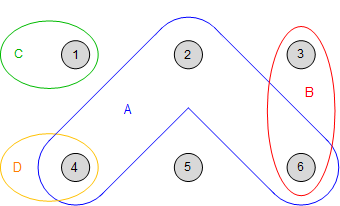
\includegraphics[width=0.5\textwidth]{Kapitel2/Bilder/image1}}
  \caption{System mit Ein- und Ausgangssignalen}
  \label{fig:EinAusSig}
\end{figure}

\noindent Einige Systeme lassen sich direkt mit algebraischen Gleichungen beschreiben. Ein Beispiel für ein solches System ist ein Spannungsteiler, bei dem sich die Ausgangsspannung direkt aus der Eingangsspannung
und dem Widerstandsverhältnis ergibt. Systeme, die sich über algebraische Gleichungen beschreiben lassen, besitzen keine Energiespeicher. Oftmals finden bei praktischen Anwendungen aber Einschwingvorgänge statt. Ursache für diese Einschwingvorgänge sind Energiespeicher, deren
Zustände sich durch eine Anregung ändern. Ein Beispiel für ein System mit Energiespeicher ist ein
RC-Tiefpass, bei dem ein Kondensator über einen Widerstand aufgeladen wird. Die Ausgangsspannung
des Kondensators ist eine Funktion der Zeit. Systeme mit Energiespeichern werden als dynamische Systeme bezeichnet. Dynamische Systeme beschreiben viele aus dem Alltag bekannte Prozesse. Beispiele sind Pendelbewegungen, das Verhalten elektrischer Schaltungen mit Kondensatoren und Spulen sowie thermische und chemische Prozesse. Es wird sich zeigen, dass die Systembeschreibung dynamischer Systeme aus einer oder mehreren Differentialgleichungen besteht.\newline
Auf Basis der mathematischen Beschreibung werden in diesem Kapitel wesentliche Systemeigenschaften
eingeführt. Diese Diskussion führt zur Untergruppe linearer, zeitinvarianter Systeme. Viele Vorgänge oder Prozesse lassen sich zumindest näherungsweise als lineare, zeitinvariante Systeme beschreiben. Die Eigenschaften Linearität und Zeitinvarianz erlauben eine vergleichsweise übersichtliche Beschreibung und vergleichsweise einfache Berechnung der Systemantwort. Dazu werden unterschiedliche
Verfahren vorgestellt.\newline
An einem Projekt mit Feder-Masse-Systemen werden lineare und nichtlineare Systeme theoretisch und experimentell miteinander verglichen.

\subsection{Beschreibung zeitkontinuierlicher Systeme mit Differentialgleichungen}\label{threeone}

Viele Systeme lassen sich über lineare Differentialgleichungen mit konstanten Koeffizienten beschreiben. In diesem Abschnitt werden einige einführende Beispiele vorgestellt.

\subsubsection{Beispiel RC-Netzwerk}
Die Beschreibung elektrischer Systeme erfolgt unter anderem über mathematische Gleichungen für die
beteiligten passiven Bauelemente. Tabelle \ref{tab:threeone} stellt die Bauelemente-Gleichungen für Widerstand, Kapazität und Induktivität zusammen [Alba04, ühr06].


\begin{table}[H]
\setlength{\arrayrulewidth}{.1em}
\caption{Thermische Bauelemente und ihre mathematische Beschreibung}
\setlength{\fboxsep}{0pt}%
\colorbox{lightgray}{%
\arrayrulecolor{white}%
\begin{tabular}{| wc{4cm} | wc{6cm} | wc{6cm} |}
\hline\xrowht{12pt}
{\fontfamily{phv}\selectfont
\textbf{Bauelement}} & 
\multicolumn{2}{c|}{\fontfamily{phv}\selectfont
\textbf{\textbf{Bauelemente-Gleichungen}}}\\ \hline \xrowht{25pt}

\fontfamily{phv}\selectfont{Widerstand} &
$U_{R}(t) = R\cdot i_{R}(t)$ &
$i_{R}(t) = \frac{1}{R}\cdot U_{R}(t)$\\ \hline  \xrowht{40pt}

\fontfamily{phv}\selectfont{Kapazität} &
$ U_{C}(t) = \frac{1}{C}\cdot \int\limits _{-\infty }^{t} i_{C}(\tau) \; d\tau$ &
$i_{C}(t) = C\cdot  \frac{dU_{C}}{dt}$\\ \hline\xrowht{40pt}

\fontfamily{phv}\selectfont{Induktivität} &
$ U_{L}(t) = L\cdot \frac{di_{L}}{dt}$ &
$i_{L}(t) = \frac{1}{L} \cdot \int\limits _{-\infty }^{t} U_{L}(\tau) \; d\tau$\\ \hline 

\end{tabular}%
}
\label{tab:threeone}
\end{table}

\bigskip

\noindent Darüber hinaus werden ideale Strom- und/oder Spannungsquellen angesetzt, die unabhängig von ihrer Belastung immer definierte Ausgangssignale liefern. Abweichungen von diesen als ideal angenommenen Quellen werden über diskrete Bauelemente wie Innenwiderstände beziehungsweise Innenleitwerte modelliert.\newline
Die Beschreibung eines Verbundes von Bauelementen erfolgt über Bilanzen und Nebenbedingungen.
Für elektrische Schaltungen ist die Bilanzgleichung bekannt als Knotengleichung.

\begin{equation}\label{eq:threeone}
\sum_{m-1}^{M}i_{m}(t)=0
\end{equation}

\noindent Die Maschengleichung stellt die entsprechende Nebenbedingung dar.

\begin{equation}\label{eq:threetwo}
\sum_{n-1}^{N}U_{n}(t)=0
\end{equation}

\noindent Bild \ref{fig:RCSchaltbild} zeigt ein einfaches Netzwerk bestehend aus einer Spannungsquelle $U_{E}(t)$, einem Widerstand R und einem Kondensator mit der Kapazität C.
\begin{figure}[ht]
  \centerline{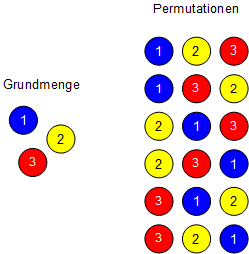
\includegraphics[width=0.32\textwidth]{Kapitel2/Bilder/image2}}
  \caption{Schaltbild für das Beispiel RC-Netzwerk}
  \label{fig:RCSchaltbild}
\end{figure}

\noindent Für das Einschalten einer Konstant-Spannungsquelle $U_{E}(t)$  soll die Spannung $U_{A}(t)$ am Kondensator berechnet werden. Die Spannung $U_{A}(t)$  wird zum Einschaltzeitpunkt $t=0$ zu $U_{A}(t)=0$ angenommen.
Dieser Zustand wird als Anfangszustand bezeichnet.

\noindent Bei der Anordnung lädt ein Strom i(t) die Kapazität C auf. Der Strom wird solange fließen, bis die Spannungsdifferenz an dem Widerstand R zu null wird. Sind die Spannungsdifferenzen ausgeglichen, befindet sich das System im Gleichgewicht. Zur mathematischen Beschreibung wird die Knotengleichung

\begin{equation}\label{eq:threethree}
i_{R}(t) = i_{C}(t) = i(t)
\end{equation}

\noindent Und die Maschengleichung

\begin{equation}\label{eq:threefour}
U_{E}(t) - U_{R}(t) - U_{A}(t)= U_{E}(t) - i_{R}(t)\cdot R - U_{A}(t) = 0
\end{equation}

\noindent aufgestellt. Wird der Strom $i_{R}(t)$ durch den Strom $i_{C}(t)$ ausgedrückt, ergibt sich

\begin{equation}\label{eq:threefive}
i_{R}(t) = i_{C}(t) = C\cdot \frac{d U_{A}}{dt}
\end{equation}

\noindent Einsetzen in die Maschengleichung führt nach Umstellen zu der linearen Differentialgleichung

\begin{equation}\label{eq:threesix}
U_{E}(t) = R\cdot C \frac{d U_{A}}{dt} + U_{A}(t)
\end{equation}

\noindent Bei der Differentialgleichung handelt es sich um eine lineare Differentialgleichung erster Ordnung mit konstanten Koeffizienten. Die Lösung dieser Differentialgleichung kann über eine sogenannte Vier-Schritt-Methode berechnet werden, auf die in Abschnitt \ref{threethree} ausführlich eingegangen wird. Bei Anregung des Systems mit einem Spannungssprung der Höhe $U_{0}$ am Eingang ergibt sich das Ausgangssignal zu

\begin{equation}\label{eq:threeseven}
U_{A}(t) = U_{0}\cdot (1-e^{\frac{t}{R\cdot C}})\cdot \sigma (t)
\end{equation}

\noindent Bild \ref{fig:RCEinschwingung} zeigt das Einschwingverhalten der Ausgangsspannung $U_{A}(t)$ für eine zum Zeitpunkt $t=0$ eingeschaltete Spannung $U_{0}= 5$ V, einen Widerstand von $R=5k\Omega$ und eine Kapazität von $C=4nF$.

\begin{figure}[ht]
  \centerline{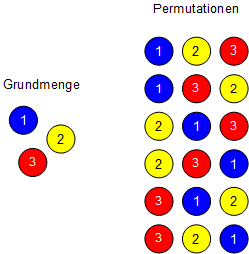
\includegraphics[width=0.5\textwidth]{Kapitel2/Bilder/image2}}
  \caption{Einschwingverhalten der Ausgangsspannung $U_{A}(t)$ eines RC-Netzwerks bei Anregung mit einem Spannungssprung von 0 auf 5 V}
  \label{fig:RCEinschwingung}
\end{figure}



\subsubsection{Beispiel Aufheizvorgang Wasserbad}
Ein Behälter, der ein Volumen V und eine Oberfläche A besitzt, ist mit Wasser gefüllt. Vereinfachend
wird angenommen, dass der Wärmeaustausch mit der Umgebung nur als Wärmeleitung über die Oberfläche
A stattfindet. Bild \ref{fig:RCEinschwingungBeispiel} beschreibt den Versuchsaufbau.

\begin{figure}[H]
  \centerline{\includegraphics[width=0.5\textwidth]{Kapitel2/Bilder/image4}}
  \caption{Aufbau für das Beispiel Tauchsieder}
  \label{fig:RCEinschwingungBeispiel}
\end{figure}

\noindent Bis zu dem Zeitpunkt t = 0 entspricht die Wassertemperatur $\vartheta _{0}$ der Umgebungstemperatur $\vartheta _{U}$. Zum Zeitpunkt t = 0 wird ein Tauchsieder in das Wasser getaucht, der eine konstante elektrische Leistung $p _{EL}(t)$ umsetzt. Der Behälter tauscht wegen seiner steigenden Temperatur$\vartheta (t)$ > $\vartheta _{U}$über die Oberfläche A Wärme mit der Umgebung aus. Die Temperatur des Wassers wird sich solange erhöhen, bis sich ein Gleichgewicht zwischen der zugeführten Leistung $p _{EL}(t)$ und des über die Fläche A abgeführten Wärmestroms $p _{A}(t)$ einstellt.
Zur Modellierung werden die Bauelemente-Gleichungen für das System aufgestellt. Bei einer Temperaturdifferenz
$\Delta \vartheta $ an einer Fläche A mit der Wärmeübergangszahl $\alpha $ strömt durch die Oberfläche A der Wärmestrom $p_{A}$

\begin{equation}\label{eq:eight}
\Delta \vartheta(t) = \vartheta (t) - \vartheta _{U} = \frac{1}{\alpha \cdot A} \cdot p_{A}(t)
\end{equation}

\noindent Diese Beschreibung ist vergleichbar zum Ohmschen Gesetz. Der elektrischen Spannung $u(t)$ entspricht bei Wärmebilanzen die Temperaturdifferenz $\Delta \vartheta (t) $, dem elektrischen Strom $i(t)$ entspricht der Wärmestrom $p _{A}(t)$. Daraus resultiert die Definition des thermischen Widerstandes $R_{TH}$ zu

\begin{equation}\label{eq:threenine}
R_{TH} = \frac{\Delta \vartheta (t)}{p _{A}(t)}=\frac{1}{\alpha \cdot A}
\end{equation}

\noindent Auch die Wärmekapazität $C_{TH}$ ist in Anlehnung an die elektrische Kapazität definiert als der Quotient aus zugeführter Leistung $dp_{C}$ und der damit verbundenen Temperaturänderung $d \vartheta$

\begin{equation}\label{eq:threeten}
C_{TH}= \frac{dp_{C}}{d_{\vartheta}}
\end{equation}

\noindent Wird Gleichung \eqref{eq:threeten} nach $d \vartheta$ aufgelöst und eine Integration über die Zeit vorgenommen, so ergibt sich für die Temperaturänderung $ \Delta \vartheta$ des Wassers

\begin{equation}\label{eq:threeelf}
\Delta \vartheta (t) = \frac{1}{d_{C_{TH}}} \cdot \int\limits _{-\infty }^{t} p_{C} (\tau) \; d\tau
\end{equation}

\noindent Tabelle \ref{tab:threetwo} fasst die thermischen Bauelemente und ihre Bauelemente-Gleichungen zusammen.

\begin{table}[H]
\setlength{\arrayrulewidth}{.1em}
\caption{Thermische Bauelemente und ihre mathematische Beschreibung}
\setlength{\fboxsep}{0pt}%
\colorbox{lightgray}{%
\arrayrulecolor{white}%
\begin{tabular}{| wc{4cm} | wc{6cm} | wc{6cm} |}
\hline\xrowht{12pt}
{\fontfamily{phv}\selectfont
\textbf{Bauelement}} & 
\multicolumn{2}{c|}{\fontfamily{phv}\selectfont
\textbf{\textbf{Bauelemente-Gleichungen}}}\\ \hline \xrowht{25pt}

\fontfamily{phv}\selectfont{Wärmewiderstand} &
$\Delta \vartheta (t)=R_{TH} \cdot p _{A}(t) = \frac{1}{\alpha \cdot A} \cdot p _{A}(t)$ &
$p _{A}(t)=\alpha \cdot A \cdot \Delta \vartheta (t)$\\ \hline \xrowht{25pt}

\fontfamily{phv}\selectfont{Wärmekapazität} &
$ U_{R}(t) = R\cdot i_{R} (t)$ &
$U_{R}(t) = R\cdot i_{R}(t) $\\ \hline 

\end{tabular}%
}
\label{tab:threetwo}
\end{table}

\noindent Für die Bilanzen gelten sinngemäß die gleichen Beziehungen wie bei den elektrischen Größen. Die Maschenregel der Temperaturdifferenzen lautet

\begin{equation}\label{eq:threetwelve}
\sum_{n-1}^{N}\Delta \vartheta _{n} (t)=0
\end{equation}

\noindent und der Knotengleichung entspricht die Leistungsbilanz

\begin{equation}\label{eq:threethirteen}
\sum_{m-1}^{M} p_{m}(t)=0
\end{equation}

\noindent Zur Verknüpfung der elektrischen und thermischen Größen wird eine Leistungsbilanz erstellt. Die elektrische Leistung $p_{EL}(t)$ wird dem System von außen zugeführt. Über die Oberfläche gibt das System eine thermische Leistung $p_{A}(t)$ ab, sobald die Wassertemperatur über die Umgebungstemperatur steigt. Die Differenz beider Leistungen $p_{C}(t)$ wird dazu verwendet, die Wassertemperatur zu erhöhen.

\begin{equation}\label{eq:threefourteen}
p_{C}(t)=p_{EL}(t)-p_{A}(t)
\end{equation}

\noindent Einsetzen der Bauelement-Gleichungen ergibt die Differentialgleichung

\begin{equation}\label{eq:threefiveteen}
C_{TH} \cdot \frac{d \Delta \vartheta}{dt}=p_{EL}(t) - \alpha\cdot A\cdot \Delta\vartheta(t)
\end{equation}

\noindent beziehungsweise

\begin{equation}\label{eq:threesixteen}
\frac{C_{TH}}{\alpha\cdot A} \cdot \frac{\Delta\vartheta(t)}{dt} + \Delta\vartheta(t) = \frac{p_{EL}(t)}{\alpha\cdot A}
\end{equation}

\noindent Sie ist eine Differentialgleichung erster Ordnung mit konstanten Koeffizienten und entspricht in ihrer Struktur der Differentialgleichung des RC-Netzwerks. Die Lösung dieser Differentialgleichung ergibt sich nach der Vier-Schritt-Methode zu

\begin{equation}\label{eq:threeseventeen}
 \Delta\vartheta(t) = \vartheta_{0}\cdot (1-e^{\frac{-t}{T}})
\end{equation}

\noindent mit der Zeitkonstanten

\begin{equation}\label{eq:threeeightteen}
T=\frac{C_{TH}}{\alpha\cdot A}
\end{equation}

\noindent und der Temperatur $\vartheta_{0}$ von

\begin{equation}\label{eq:threenineteen}
\vartheta_{0} = \frac{p_{EL}(t)}{\alpha\cdot A}
\end{equation}

\noindent Bild \ref{fig:TempEinschwingung} stellt das Einschwingverhalten für eine Zeitkonstante T = 5 s und einen Temperatursprung $\vartheta_{0}$ von 20 K dar. Es entspricht grundsätzlich dem Einschwingverhalten des RC-Netzwerks.

\begin{figure}[H]
  \centerline{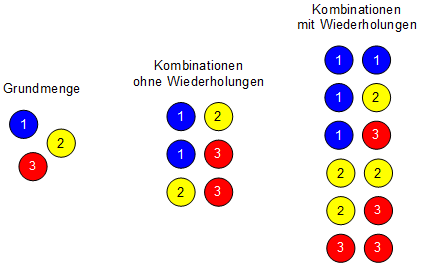
\includegraphics[width=1\textwidth]{Kapitel2/Bilder/image5}}
  \caption{Einschwingverhalten der Temperaturdifferenz bei einer sprungförmigen Anregung\\ mit einer konstanten elektrischen Leistung
}
  \label{fig:TempEinschwingung}
\end{figure}

\subsubsection{Beispiel Feder-Masse-Dämpfer-System}
Als weiteres Beispiel wird ein Feder-Masse-Dämpfer-System betrachtet, auf das eine äußere Kraft $F_{E}$ ausgeübt wird. Bild \ref{fig:FDSBeispiel} zeigt schematisch die Anordnung. Die Kraft $F_{E}$ greift an einem Körper der Masse m an und bewegt den Körper. Der Bewegung stehen die Trägheits-, Dämpfungs- und Rückstellkraft der Feder entgegen. Für die Anordnung soll die Auslenkung x berechnet werden, die sich bei
einer sprungförmig aufgebrachten Kraft FE an der Feder ergibt.

\begin{figure}[ht]
  \centerline{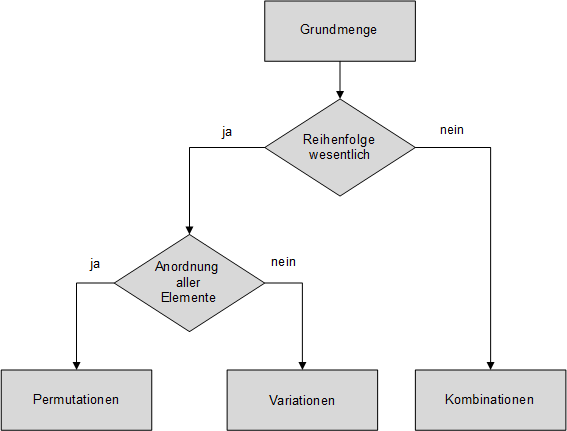
\includegraphics[width=0.5\textwidth]{Kapitel2/Bilder/image6}}
  \caption{Beispiel Feder-Dämpfer-System}
  \label{fig:FDSBeispiel}
\end{figure}

\noindent Genau wie bei dem elektrischen System lassen sich die mechanischen Bauelemente isoliert beschreiben. Tabelle \ref{tab:threethree} fasst mechanisch translatorische Bauelemente und ihre mathematische Beschreibung
zusammen.

\begin{table}[H]
\setlength{\arrayrulewidth}{.1em}
\caption{Thermische Bauelemente und ihre mathematische Beschreibung}
\setlength{\fboxsep}{0pt}%
\colorbox{lightgray}{%
\arrayrulecolor{white}%
\begin{tabular}{| wc{5.5cm} | wc{5.2cm} | wc{5.2cm} |}
\hline\xrowht{15pt}
{\fontfamily{phv}\selectfont
\textbf{Bauelement}} & 
\multicolumn{2}{c|}{\fontfamily{phv}\selectfont
\textbf{\textbf{Bauelemente-Gleichungen}}}\\ \hline \xrowht{40pt}

\fontfamily{phv}\selectfont{Feder mit Federkonstante c} &
$F_{C} \left(t\right)=c\cdot \int\limits _{-\infty }^{t}v\left(\tau \right){\rm \; }d\tau  =c\cdot x\left(t\right)$ & $v\left(t\right)=\frac{1}{c} \cdot \frac{dF_{C} }{dt} $ \\ \hline \xrowht{40pt}

\fontfamily{phv}\selectfont{Masse m} &
$F_{M} \left(t\right)=m\cdot a\left(t\right)=m\cdot \frac{dv}{dt} $ & $v\left(t\right)=\frac{1}{m} \cdot \int\limits _{-\infty }^{t}F_{M} \left(\tau \right){\rm \; }d\tau  $ \\ \hline\xrowht{40pt}

\fontfamily{phv}\selectfont{Viskose Reibung / Dämpfer D} &
$F_{D} \left(t\right)=D\cdot v\left(t\right)=D\cdot \frac{dx}{dt} $ & $v\left(t\right)=\frac{1}{D} \cdot F_{D} \left(t\right)$\\ \hline\xrowht{40pt}

\fontfamily{phv}\selectfont{Gleitreibung} & 
$F_{G} \left(t\right)=\mu \cdot F_{N} \left(t\right)\cdot sgn\left(v\left(t\right)\right)$ & \fontfamily{phv}\selectfont{keine Invertierung möglich} \\ \hline 
\end{tabular}%
}
\label{tab:threethree}
\end{table}


\noindent Auch in der Mechanik werden Gleichungen angesetzt, die den Maschen- und Knotenregeln entsprechen. Der Maschenregel entspricht die Kräftesumme

\begin{equation}\label{eq:threetwenty}
\sum_{n-1}^{N} F_{n}(t)=0
\end{equation}

\noindent Durch mechanische Kopplung lässt sich eine Aussage über die Auslenkung der verschiedenen Bauelemente des Systems machen. In diesem Beispiel sind Masse, Feder und Dämpfer starr miteinander gekoppelt. Die Auslenkungen x(t) für Masse, Feder und Dämpfer sind damit identisch. Die Anwendung der Kräftebilanz ergibt unter Berücksichtigung der unterschiedlichen Kraftrichtungen

\begin{equation}\label{eq:threetwentyone}
F_{E}(t)-F_{M}(t)-F_{D}(t)-F_{C}(t)=
F_{E}(t)-m\cdot a(t)-D\cdot v(t)-c\cdot x(t)=0
\end{equation}

\noindent und der Zusammenhang zwischen der Auslenkung $x(t)$ und der angreifenden Kraft $F_{E}(t)$ kann als Differentialgleichung dargestellt werden.

\begin{equation}\label{eq:threetwentytwo}
F_{E}(t)=m\cdot \frac{d^2x}{dt^2}+D\cdot \frac{dx}{dt}+c\cdot x(t)
\end{equation}

\noindent Es handelt sich wieder um eine lineare Differentialgleichung mit konstanten Koeffizienten. Die Ordnung der Differentialgleichung entspricht der höchsten Ableitung, in diesem Beispiel ist die Ordnung N = 2. Die Lösung der Differentialgleichung kann für ein definiertes Eingangssignal und eine definierte Anfangsbedingung wie bei dem elektrischen System mit der Vier-Schritt-Methode erfolgen. Für ein System, das sich zum Zeitpunkt t = 0 in Ruhelage befindet und mit einem Kraftsprung am Eingang

\begin{equation}\label{eq:threetwentythree}
F_{E}(t)=F_{0}\cdot \sigma(t)
\end{equation}

\noindent angeregt wird, ergibt sich bei geringer Dämpfung D die Lösung


\begin{equation}\label{eq:threetwentyfour}
x(t) = \frac{F_{0}}{c} \cdot \left(1+\frac{e^{-\frac{D}{2\cdot m} \cdot t} }{\sqrt{1-\left(\frac{D}{2\cdot \sqrt{m\cdot c} } \right)^{2} } } \cdot \sin \left(\sqrt{\frac{c}{m} -\left(\frac{D}{2\cdot m} \right)^{2} } \cdot t-\varphi \right)\right)\cdot \sigma \left(t\right)
\end{equation}

\noindent Auf die Berechnung dieses  inschwingverhaltens wird später noch genauer eingegangen. Das Einschwingverhalten ist in Bild \ref{fig:AusblendeigenschaftImpulsfunktion} für eine Federkonstante von c = 100 N/m, eine Dämpfung von $D = 0.5 N\cdot s/m$, eine Masse m = 10 g und eine Kraft $F_{0}= 0.2 N$  dargestellt.

\begin{figure}[ht]
  \centerline{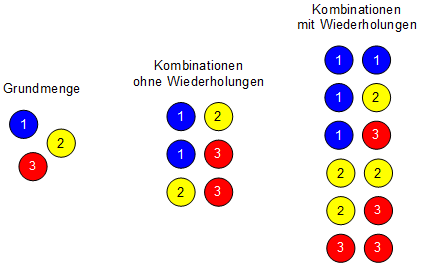
\includegraphics[width=1\textwidth]{Kapitel2/Bilder/image5}}
  \caption{Einschwingverhalten des Feder-Masse-Dämpfer-Systems bei einer sprungförmigen Anregung mit einer Kraft von $F_{0}= 0.2 N$}
  \label{fig:AusblendeigenschaftImpulsfunktion}
\end{figure}

\subsubsection{Resümee zu den Beispielen}
Viele Systeme lassen sich wie die hier diskutierten Systeme zumindest in guter Näherung durch lineare
Differentialgleichungen mit konstanten Koeffizienten beschreiben.

\begin{equation}\label{eq:threetwentyfive}
a_{0}\cdot y(t) + a_{1}\cdot \frac{dy}{dt}+a_{2}\cdot \frac{d^2y}{dt^2}+ ... +a_{n}\cdot \frac{d^Ny}{dt^N}=
b_{0}\cdot u(t) + b_{1}\cdot \frac{du}{dt}+b_{2}\cdot \frac{d^2u}{dt^2}+ ... +b_{m}\cdot \frac{d^Mu}{dt^M}
\end{equation}

\noindent Die Beschreibung des Systems mit Differentialgleichungen wird als Modellbildung bezeichnet. Sie ist für praktische Aufgabenstellungen anspruchsvoll und oft nur mit Erfahrung zu lösen. Auf die Modellbildung wird in Kapitel \textbf{Fehler! Verweisquelle konnte nicht gefunden werden}. ausführlich eingegangen, und es wird ein Leitfaden zur Modellierung von Systemen vorgestellt.


\subsection{Grundlegende Eigenschaften zeitkontinuierlicher Systeme} \label{threetwo}

Im Abschnitt \ref{threeone} werden unterschiedliche Systeme beschrieben. Die mathematische Modellierung führt bei diesen Beispielen zu linearen Differentialgleichungen mit konstanten Koeffizienten. In diesem Abschnitt werden grundlegende Eigenschaften von Systemen diskutiert. Es wird sich zeigen, dass lineare Differentialgleichungen mit konstanten Koeffizienten lineare, zeitinvariante Systeme beschreiben.

\subsubsection{Linearität}
Für den Linearitätsnachweis eines Systems müssen die Systemantworten $y_{1}(t)$ und $y_{2}(t)$ auf die linear unabhängigen Eingangssignale $u_{1}(t)$ und $u_{2}(t)$ bekannt sein. Ein System ist linear, wenn es auf eine Linearkombination von Eingangssignalen

\begin{equation}\label{eq:threetwentysix}
u_{t} = v_{1}\cdot u_{1}(t) +v_{2}\cdot u_{2}(t)
\end{equation}

\noindent mit derselben Linearkombination der entsprechenden Kombination von Ausgangssignalen reagiert.

\begin{equation}\label{eq:threetwentyseven}
y_{t} = v_{1}\cdot y_{1}(t) +v_{2}\cdot y_{2}(t)
\end{equation}

\noindent Der Nachweis der Linearität erfolgt über Einsetzen der Gleichungen in die Differentialgleichung.\bigskip

\noindent
\colorbox{lightgray}{%
\arrayrulecolor{white}%
\renewcommand\arraystretch{0.6}%
\begin{tabular}{ wl{16.5cm} }
{\fontfamily{phv}\selectfont{Beispiel: Linearität eines RC-Netzwerks} }
\end{tabular}%
}\bigskip

\noindent Ein RC-Netzwerk mit der Differentialgleichung

\begin{equation}\label{eq:threetwentyeight}
U_{E}(t) =R\cdot C\cdot \frac{dU_{A}(t)}{dt}+ U_{A}(t)
\end{equation}

\noindent soll auf Linearität untersucht werden. Die Systemantworten $U_{A1}(t)$ und $U_{A2}(t)$ ergeben sich mit der Differentialgleichung \ref{eq:threetwentyeight} zu

\begin{equation}\label{eq:threetwentynine}
U_{E1}(t) =R\cdot C\cdot \frac{dU_{A1}(t)}{dt}+ U_{A1}(t)
\end{equation}

\noindent beziehungsweise

\begin{equation}\label{eq:threethirty}
U_{E2}(t) =R\cdot C\cdot \frac{dU_{A2}(t)}{dt}+ U_{A2}(t)
\end{equation}

\noindent Wird das System mit der Linearkombination

\begin{equation}\label{eq:threethirtyone}
U_{E}(t) =\nu_{1}\cdot U_{E1}(t) +\nu_{2}\cdot U_{E2}(t)
\end{equation}

\noindent angeregt, ergibt sich

\begin{equation}\label{eq:threethirtytwo}
\begin{split} 
u_{E} \left(t\right) & = \nu _{1} \cdot u_{E1} \left(t\right)+\nu _{2} \cdot u_{E2} \left(t\right) \\ 
& = \nu _{1} \cdot \left(R\cdot C\cdot \frac{du_{A1} \left(t\right)}{dt} +u_{A1} \left(t\right)\right)+\nu _{2} \cdot \left(R\cdot C\cdot \frac{du_{A2} \left(t\right)}{dt} +u_{A2} \left(t\right)\right) \\ 
& = R\cdot C\cdot \left(\nu _{1} \cdot \frac{du_{A1} \left(t\right)}{dt} +\nu _{2} \cdot \frac{du_{A2} \left(t\right)}{dt} \right)+\left(\nu _{1} \cdot u_{A1} \left(t\right)+\nu _{2} \cdot u_{A2} \left(t\right)\right) \\ 
& = R\cdot C\cdot \frac{du_{A} \left(t\right)}{dt} +u_{A} \left(t\right) 
\end{split}
\end{equation}

\noindent Das Ausgangssignal $U_{A}(t)$ weist dieselbe Linearkombination auf wie das Eingangssignal.


\noindent
\colorbox{lightgray}{%
\arrayrulecolor{white}%
\renewcommand\arraystretch{0.6}%
\begin{tabular}{ wl{16.5cm} }
{\fontfamily{phv}\selectfont{Beispiel: Nichtlineares System}}
\end{tabular}%
}\bigskip

\noindent Der Strom $i_{D}(t)$  durch eine Diode als Funktion der anliegenden Spannung wird über die Shockley-Gleichung berechnet.

\begin{equation}\label{eq:threethirtythree}
i_{D}(t)=I_{S}\cdot (e^{\frac{U_{D}(t)}{n\cdot U_{T}}}-1)
\end{equation}

\noindent Die Diode soll auf Linearität untersucht werden. Die Systemantworten $i_{D1}(t)$  und $i_{D2}(t)$ ergeben sich mit der Shockley-Gleichung zu

\begin{equation}\label{eq:threethirtyfour}
i_{D1}(t)=I_{S}\cdot (e^{\frac{U_{D1}(t)}{n\cdot U_{T}}}-1)
\end{equation}

\noindent beziehungsweise

\begin{equation}\label{eq:threethirtyfive}
i_{D2}(t)=I_{S}\cdot (e^{\frac{U_{D2}(t)}{n\cdot U_{T}}}-1)
\end{equation}

\noindent Wird das System mit der Linearkombination

\begin{equation}\label{eq:threethirtysix}
U_{D}(t)=k_{1}\cdot U_{D1}(t) + k_{2}\cdot U_{D2}(t) 
\end{equation}

\noindent angeregt, ergibt sich der Diodenstrom

\begin{equation}\label{eq:threethirtyseven}
\begin{split}
i_{D}(t) & = I_{S} \cdot \left(e^{\frac{u_{D} \left(t\right)}{n\cdot U_{T} } } -1\right)=I_{S} \cdot \left(e^{\frac{\nu _{1} \cdot u_{D1} \left(t\right)+\nu _{2} \cdot u_{D2} \left(t\right)}{n\cdot U_{T} } } -1\right)=I_{S} \cdot \left(e^{\frac{\nu _{1} \cdot u_{D1} \left(t\right)}{n\cdot U_{T} } } \cdot e^{\frac{\nu _{2} \cdot u_{D2} \left(t\right)}{n\cdot U_{T} } } -1\right) \\ 
& \ne \nu _{1} \cdot I{}_{S} \cdot \left(e^{\frac{u_{D1} \left(t\right)}{n\cdot U_{T} } } -1\right)+\nu _{2} \cdot I{}_{S} \cdot \left(e^{\frac{u_{D2} \left(t\right)}{n\cdot U_{T} } } -1\right) = \nu _{1} \cdot i_{D1} \left(t\right)+\nu _{2} \cdot i_{D2} \left(t\right)
\end{split}
\end{equation}

\noindent Der Strom $i_{D}(t)$  durch die Diode ist nichtlinear zur Spannung $u_{D}(t)$, die an der Diode anliegt. Eine Diode ist damit ein nichtlineares Bauteil.\newline
Die Linearität von Systemen kann auch daran abgelesen werden, dass alle Signale und Ableitungen nur in linearen Summen auftreten. Ist ein System linear, kann ein Ausgangssignal dadurch berechnet werden, dass die Eingangssignale zerlegt, ihre jeweiligen Systemantworten berechnet und anschließend addiert werden. Dieses Prinzip wird als Superpositionsprinzip bezeichnet. Bild 3.8 zeigt Ein- und Ausgangssignale eines linearen Systems, das mit den Signalen $u_{1}(t)$, $u_{2}(t)$ und $u_{1}(t)$ + $u_{2}(t)$ angeregt wird. Das Ausgangssignal $y(t)$ setzt sich aus der Summe der Ausgangsignale $y_{1}(t)$ und $y_{2}(t)$ zusammen.

\begin{figure}[H]
  \centerline{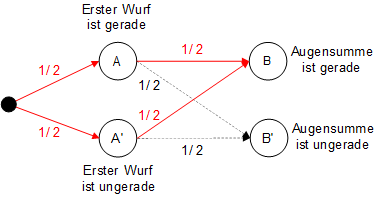
\includegraphics[width=1\textwidth]{Kapitel2/Bilder/image8}}
  \caption{Reaktion eines linearen Systems auf die Anregung mit einer Linearkombination von Signalen}
  \label{fig:Linearitat}
\end{figure}

\noindent Linearität ist eine idealisierte Eigenschaft eines Systems, zum Beispiel wird sich der Widerstand R nichtlinear verhalten, wenn in ihm eine hohe Verlustleistung umgesetzt wird, und er sich erhitzt. In der Praxis werden viele Prozesse oder Systeme linear beschrieben, obwohl diese idealisierte Annahme nur in definierten Grenzen gilt. Andererseits können auch nichtlineare Systeme näherungsweise linear beschrieben werden. Dazu wird in dem nichtlinearen System ein Arbeitspunkt definiert und kleine Abweichungen aus dem Arbeitspunkt werden als linear angenommen.\bigskip

\noindent
\colorbox{lightgray}{%
\arrayrulecolor{white}%
\renewcommand\arraystretch{0.6}%
\begin{tabular}{ wl{16.5cm} }
{\fontfamily{phv}\selectfont
{Beispiel: Linearisierung einer Diodenkennlinie im Arbeitspunkt}}
\end{tabular}%
}\bigskip

\noindent Das nichtlineare Verhalten des Diodenstroms $i_{D}(t)$  als Funktion der Diodenspannung $u_{D}(t)$ soll in einem Arbeitspunkt mit der Spannung $u_{0}$ und dem Strom $i_{0}$ linearisiert werden. Bild \ref{fig:Linearisierung} verdeutlicht die Linearisierung um einen Arbeitspunkt grafisch.\bigskip

\begin{figure}[H]
  \centerline{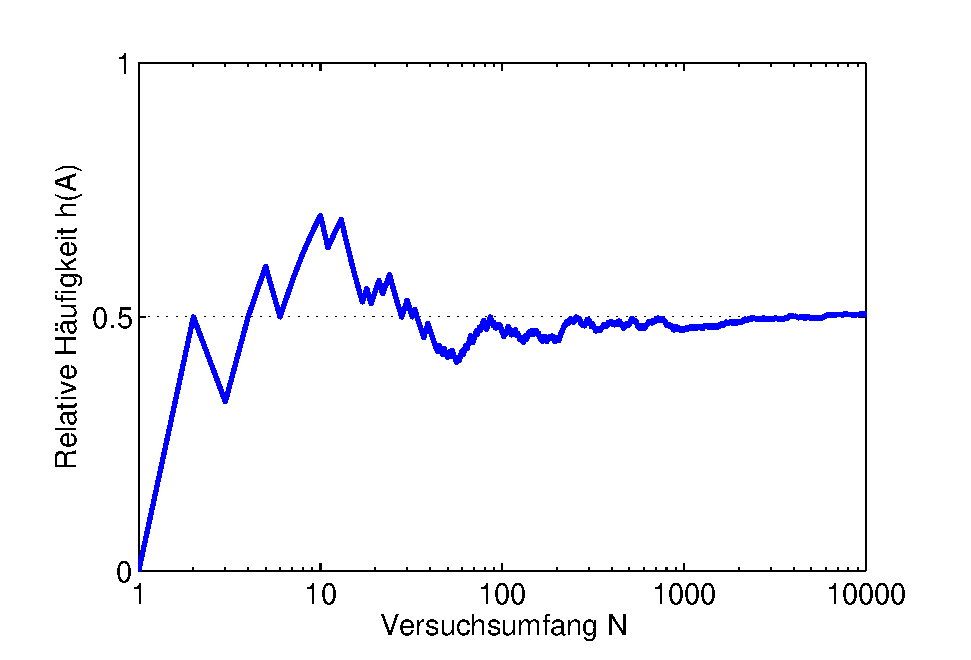
\includegraphics[width=0.5\textwidth]{Kapitel2/Bilder/image9}}
  \caption{Linearisierung um einen Arbeitspunkt am Beispiel der Diodenkennlinie}
  \label{fig:Linearisierung}
\end{figure}

\noindent In dem Arbeitspunkt $(u_{0}|i_{0})$ wird durch Ableitung der Shockley-Gleichung die Steigung der Tangente bestimmt.


\begin{equation}\label{eq:threethirtyeight}
m=\left. \frac{di_{D} }{du_{D} } \right|_{u_{D} =u_{0} } =\left. \frac{I_{S} }{n\cdot U_{T} } \cdot e^{\frac{u_{D} \left(t\right)}{n\cdot U_{T} } } \right|_{u_{D} =u_{0} } =\frac{I_{S} }{n\cdot U_{T} } \cdot e^{\frac{u_{0} }{n\cdot U_{T} } }
\end{equation}

\noindent Das Systemverhalten im Arbeitspunkt ergibt sich dann aus der Geradengleichung


\begin{equation}\label{eq:threethirtynine}
i_{D} \left(t\right)-i_{0} =\frac{I_{S} }{n\cdot U_{T} } \cdot e^{\frac{u_{0} }{n\cdot U_{T} } } \cdot \left(u_{D} \left(t\right)-u_{0} \right)=m\cdot \left(u_{D} \left(t\right)-u_{0} \right)
\end{equation}

\noindent Mit den Bezeichnungen

\begin{equation}\label{eq:threefourty}
\Delta i_{D}(t)=i_{D}(t)-i_{0}
\end{equation}

\begin{equation}\label{eq:threefourtyone}
\Delta U_{D}(t)=U_{D}(t)-U_{0}
\end{equation}

\noindent ergibt sich die lineare Beschreibungsform

\begin{equation}\label{eq:threefourtytwo}
\Delta i_{D}(t)=m\cdot \Delta U_{D}(t)
\end{equation}

\noindent Gleichung \ref{eq:threefourtytwo} stellt eine lineare Näherung für das nichtlineare System Diode im Arbeitspunkt $(u_{0}|i_{0})$ dar. Bild \ref{fig:Linearisierung} macht jedoch deutlich, dass diese Linearisierung nur für sehr kleine Werte $\Delta u_{D}$ ausreichend präzise ist.

\subsubsection{Zeitinvarianz}\label{threetwotwo}
Ein System reagiert auf ein Eingangssignal $u(t)$ mit einer Systemantwort $y(t)$. Ist das System zeitinvariant, so reagiert das System auf das zeitlich verschobene  Eingangssignal $u(t-t_{0})$ mit dem verschobenen Ausgangsignal $y(t-t_{0})$. Zeitinvariante Systeme reagieren also unabhängig vom Startzeitpunkt der Anregung auf gleiche Eingangssignale mit gleichen Ausgangssignalen.\bigskip

\noindent
\colorbox{lightgray}{%
\arrayrulecolor{white}%
\renewcommand\arraystretch{0.6}%
\begin{tabular}{ wl{16.5cm} }
{\fontfamily{phv}\selectfont{Beispiel: Zeitinvarianz eines Feder-Masse-Dämpfer Systems }}
\end{tabular}%
}\bigskip

\noindent Das Feder-Masse-Dämpfer System mit der Differentialgleichung

\begin{equation}\label{eq:threefourtythree}
F_{E}(t)= m\cdot \frac{d^2x}{dt^2}+D\cdot \frac{dx}{dt} + c\cdot x(t)
\end{equation}

\noindent soll auf Zeitinvarianz untersucht werden. Dazu werden alle Ausdrücke t durch den Ausdruck $t - t_{0}$ ersetzt. Unter der Annahme, dass die Koeffizienten m, D und c nicht ändern, ergibt sich die Differentialgleichung

\begin{equation}\label{eq:threefourtyfour}
F_{E}(t-t_{0})= m\cdot \frac{d^2x(t-t_{0})}{dt^2}+D\cdot \frac{dx(t-t_{0})}{dt} + c\cdot x(t-t_{0})
\end{equation}

\noindent Wird das Eingangssignal um $t_{0}$ verschoben, wird auch das Ausgangsignal um $t_{0}$ verschoben.
\clearpage
\begin{figure}[H]
  \centerline{\includegraphics[width=1\textwidth]{Kapitel2/Bilder/image10}}
  \caption{Reaktion eines zeitinvarianten Systems auf die Anregung mit einem um $t_{0} = 0.2 s$\\ zeitverschobenen Signal} 
  \label{fig:Zeitinvarianz}
\end{figure}

\noindent Wird ein System mit einer linearen Differentialgleichung beschrieben, die konstante Koeffizienten
aufweist, ist das Systemverhalten von der Zeit unabhängig, und das System ist zeitinvariant. Ändern sich die Koeffizienten der Differentialgleichung als Funktion der Zeit t, verändert sich das System mit der Zeit. Es ist zeitvariant.\newline
Auch die Zeitinvarianz ist eine Eigenschaft, die oft nur näherungsweise erfüllt ist. Zum Beispiel werden bei einem linearen RLC-Netzwerk die Bauelemente-Parameter über die Lebensdauer geringfügig driften. Damit wird aus einem konstanten Widerstand R ein von der Zeit abhängiger Widerstand R(t), das System verändert sich. Typischerweise sind diese Änderungsprozesse aber viel langsamer als die Signaländerungen der Schaltung, die berechnet werden sollen, und können deshalb vernachlässigt werden.

\subsubsection{Lineare, zeitinvariante Systeme (LTI-Systeme)}\label{threetwothree}

Systeme, die sowohl linear, als auch zeitinvariant sind, werden als LTI-Systeme bezeichnet. Die Bezeichnung leitet sich von dem englischen Begriff \textit{Linear-Time-Invariant-System } ab. Bild \ref{fig:Zeitinvarianzsys} stellt die beiden Forderungen nach Linearität und Zeitinvarianz grafisch zusammen:


\begin{figure}[H]
  \centerline{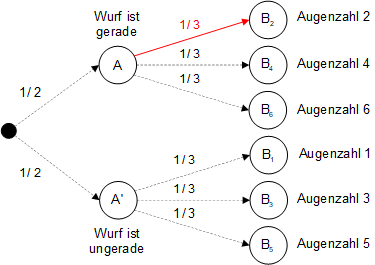
\includegraphics[width=0.5\textwidth]{Kapitel2/Bilder/image11}}
  \caption{Lineares zeitinvariantes System} 
  \label{fig:Zeitinvarianzsys}
\end{figure}

\noindent Für LTI-Systeme sind vergleichsweise anschauliche und einfach zu interpretierende Lösungs- und Interpretationsmethoden im Zeit- und Frequenzbereich vorhanden. Die Darstellungen in diesem Buch beschränken sich bis auf wenige Ausnahmen auf LTI-Systeme.\newline
Systeme, die mit einer linearen Differentialgleichung mit konstanten Koeffizienten beschrieben werden können, erfüllen die Bedingungen nach Linearität und Zeitinvarianz. Ausgehend von der allgemeinen Differentialgleichung

\begin{equation}\label{eq:threefourtyfive}
a_{0}\cdot y(t) + a_{1}\cdot \frac{dy}{dt}+a_{2}\cdot \frac{d^2y}{dt^2}+ ... +a_{n}\cdot \frac{d^Ny}{dt^N}=
b_{0}\cdot u(t) + b_{1}\cdot \frac{du}{dt}+b_{2}\cdot \frac{d^2u}{dt^2}+ ... +b_{m}\cdot \frac{d^Mu}{dt^M}
\end{equation}

\noindent beziehungsweise ihrer Darstellung als Summenformel

\begin{equation}\label{eq:threefourtysix}
\sum_{n=0}^{N}a_{n} \cdot  \frac{d^ny}{dt^n} =
\sum_{m=0}^{M}b_{m} \cdot  \frac{d^mu}{dt^m}
\end{equation}

\noindent werden die Eigenschaften der Linearität und Zeitinvarianz nachgewiesen.\bigskip

{\fontfamily{phv}\selectfont\noindent \textbf{Linearität}}\smallskip

\noindent Ausgangspunkt für den Beweis der Linearität sind zwei Signalkombinationen $u_{1}(t)$  und $y_{1}(t)$ sowie $u_{2}(t)$ und $y_{2}(t)$, für die gilt:

\begin{equation}\label{eq:threefourtyseven}
\sum_{n=0}^{N}a_{n} \cdot  \frac{d^ny_{1}}{dt^n} =
\sum_{m=0}^{M}b_{m} \cdot  \frac{d^mu_{1}}{dt^m}
\end{equation}

\begin{equation}\label{eq:threefourtyeight}
\sum_{n=0}^{N}a_{n} \cdot  \frac{d^ny_{2}}{dt^n} =
\sum_{m=0}^{M}b_{m} \cdot  \frac{d^mu_{1}}{dt^m}
\end{equation}

\noindent Ist das System linear, muss die Differentialgleichung bei einer Kombination von Eingangssignalen

\begin{equation}\label{eq:threefourtynine}
u(t)=v_{1}\cdot u_{1}(t)+v_{2}\cdot u_{2}(t)
\end{equation}

\noindent mit derselben Linearkombination der Ausgangssignale

\begin{equation}\label{eq:threefifty}
y(t)=v_{1}\cdot y_{1}(t)+v_{2}\cdot y_{2}(t)
\end{equation}

\noindent erfüllt sein. Einsetzen der Gleichungen führt zu

\begin{equation}\label{eq:threefiftyone}
\begin{split}
\sum _{n=0}^{N}a_{n} \cdot \frac{d^{n} y}{dt^{n} }   & = \sum _{n=0}^{N}a_{n} \cdot \frac{d^{n} \left(\nu _{1} \cdot y_{1} \left(t\right)+\nu _{2} \cdot y_{2} \left(t\right)\right)}{dt^{n} }  =\sum _{n=0}^{N}a_{n} \cdot \nu _{1} \cdot \frac{d^{n} y_{1} }{dt^{n} } +a_{n} \cdot \nu _{2} \cdot \frac{d^{n} y_{2} }{dt^{n} }  + \\ 
& =\nu _{1} \cdot \sum _{n=0}^{N}a_{n} \cdot \frac{d^{n} y_{1} }{dt^{n} }  +\nu _{2} \cdot \sum _{n=0}^{N}a_{n} \cdot \frac{d^{n} y_{2} }{dt^{n} }  =\nu _{1} \cdot \sum _{m=0}^{M}b_{m} \cdot \frac{d^{m} u_{1} }{dt^{m} }  +\nu _{2} \cdot \sum _{m=0}^{M}b_{m} \cdot \frac{d^{m} u_{2} }{dt^{m} }\\ 
& = \sum _{m=0}^{M}b_{m} \cdot \nu _{1}  \cdot \frac{d^{m} u_{1} }{dt^{m} } + b_{m} \nu _{2} \cdot \frac{d^{m} u_{2} }{dt^{m}} = \sum _{m=0}^{M}b_{m} \cdot \frac{d^{m} \left(\nu _{1} \cdot y_{1} \left(t\right)+\nu _{2} \cdot y_{2} \left(t\right)\right)}{dt^{m} }\\
& = \sum _{m=0}^{M}b_{m} \cdot \frac{d^{m}u}{dt^{m}}
\end{split}
\end{equation}

\noindent Eine Linearkombination von Eingangssignalen führt damit zu der identischen Linearkombination von Ausgangssignalen, sodass das System ein lineares System ist. \bigskip

{\fontfamily{phv}\selectfont
\noindent\textbf{Zeitinvarianz}}\smallskip

\noindent Das System wird mit einer Differentialgleichung mit konstanten Koeffizienten beschrieben. Damit ist das Systemverhalten von der Zeit unabhängig, und das System ist zeitinvariant.

\subsubsection{Kausalität}

\noindent Hängt das Ausgangssignal $y(t)$ eines Systems zu einem Zeitpunkt $t_{1}$ nur von Eingangswerten $u(t)$ mit $t \leqslant  t_{1}$ ab, wird das System als kausales System bezeichnet. Physikalisch sinnvolle und realisierbare Systeme sind wegen des Ursachewirkungsprinzips kausal.\bigskip

\noindent
\colorbox{lightgray}{%
\arrayrulecolor{white}%
\renewcommand\arraystretch{0.6}%
\begin{tabular}{ wl{16.5cm} }
Beispiel: Aufheizvorgang Wasserbad 
\end{tabular}%
}\bigskip

\noindent Aus der Erfahrung im Umgang mit Aufheizvorgängen ist bekannt, dass sich die Temperatur in einem Wasserbad erst dann erhöht, wenn eine Heizung eingeschaltet wird. Die Kausalität ergibt sich auch aus der mathematischen Beschreibung.

\begin{equation}\label{eq:threefiftytwo}
\frac{C_{TH}}{\alpha\cdot A} \cdot \frac{\Delta\vartheta(t)}{dt} + \Delta\vartheta(t) = \frac{p_{EL}(t)}{\alpha\cdot A}
\end{equation}

\noindent Erst wenn elektrische Leistung $p_{EL}(t)$ in das System eingespeist wird, ändert sich die Temperatur
$\Delta\vartheta(t)$.\bigskip

\noindent
\colorbox{lightgray}{%
\arrayrulecolor{white}%
\renewcommand\arraystretch{0.6}%
\begin{tabular}{ wl{16.5cm} }
Beispiel: Differenzierer als nicht kausales System
\end{tabular}%
}\bigskip

\noindent Die Differentiation eines Signals u(t) kann mathematisch beschrieben werden als

\begin{equation}\label{eq:threefiftythree}
y(t) = \frac{du}{dt} \approx \frac{u\left(t+\Delta t\right)-u\left(t-\Delta t\right)}{2\cdot \Delta t} 
\end{equation}

\noindent Zur Berechnung der Ableitung werden Eingangssignale verwendet, die in der Zukunft liegen. Ein Differenzierer ist damit kein kausales System.

\subsubsection{Stabilität}

Zur Erklärung des Begriffes der Stabilität wird von einem physikalischen Gedankenexperiment ausgegangen.
Eine Kugel liegt auf einer Fläche, die unterschiedliche Krümmungen aufweist. In allen Fällen liegt die Kugel zunächst in einer Ruhelage, die mit x = 0 bezeichnet wird. Die Kugel wird aus dieser Ruhelage um $x_{0}$  ausgelenkt und danach sich selber überlassen.

\begin{figure}[H]
  \centerline{\includegraphics[width=1\textwidth]{Kapitel2/Bilder/image12}}
  \caption{Gedankenmodell zur Erklärung des Stabilitätsbegriffes}
  \label{fig:StabilitaetErklaerung}
\end{figure}

\noindent Im Fall a wirkt auf die Kugel nach der Auslenkung eine tangentiale Kraftkomponente, die sie in Richtung der Ruhelage beschleunigt. In der Stelle x = 0 wird die Kraftkomponente zu null, die Kugel besitzt jedoch eine Geschwindigkeit $v_{0}$  und überstreicht die Ruhelage. Lageenergie wird in kinetische
Energie gewandelt und umgekehrt. Aufgrund der Reibung und des Luftwiderstandes gibt die Kugel Energie an die Umgebung ab, die Auslenkung wird kleiner und schließlich gelangt die Kugel wieder
in die Ruhelage x = 0. Das System wird als asymptotisch stabil bezeichnet. Im Fall b wird die Kugel nach einer einmaligen Auslenkung $x_{0}$ dort liegen bleiben, da sie keine Kraft erfährt, die tangential auf sie wirkt. Da die Kugel nicht mehr in ihre Ruhelage zurückkehrt, ist das System nicht asymptotisch stabil, die Auslenkung der Kugel steigt aber auch nicht an. Das System wird deshalb als grenzstabil bezeichnet. Im Fall c wird die Kugel nach einer Auslenkung um $x_{0}$ die Fläche herunterrollen, mit steigender Auslenkung nimmt die tangentiale Kraftkomponente zu. Wegen der steigenden Auslenkung wird das System als instabil bezeichnet.\newline
Aus diesem Gedankenexperiment ergibt sich eine physikalische Stabilitätsdefinition: Ein System ist asymptotisch stabil, wenn es nach einer Anregung mit endlicher Energie wieder seine Ruheposition erreicht. Es ist grenzstabil, wenn es nach Anregung mit endlicher Energie zu einem konstanten Ausgangswert konvergiert, und es ist instabil, wenn es auf eine Anregung endlicher Energie mit divergierendem Ausgangssignal reagiert.\newline
Diese physikalische Stabilitätsdefinition ist zwar anschaulich, jedoch praktisch schlecht auszuwerten. Deshalb wird der Stabilitätsbegriff bei der Diskussion der charakteristischen Gleichung in Abschnitt \ref{threethreetwo} und des Faltungsintegrals in Abschnitt \ref{threefourfive} erneut aufgegriffen.

\subsubsection{Systeme mit und ohne Ausgleich}

\noindent Zur Interpretation von Systemen ist die Frage wichtig, ob das vorliegende System ein System mit oder ohne Ausgleich ist. Zur Einführung wird das Beispiel des Aufheizvorgangs aufgegriffen. Der Aufheizvorgang wird über die Differentialgleichung

\begin{equation}\label{eq:threefiftyfour}
p_{EL}(t) = C_{TH}\cdot \frac{\Delta\vartheta(t)}{dt}+ \alpha\cdot A \cdot \Delta\vartheta(t)
\end{equation}

\noindent beschrieben. Bei Einschalten des Tauchsieders wird elektrische Leistung $p_{EL}(t)$ in Wärme umgewandelt.
Es ergibt sich eine Temperaturerhöhung $\Delta\vartheta(t)$. Diese Temperaturerhöhung führt wiederum zu einer größeren Wärmeabgabe an die Umgebung. Es stellt sich ein stationärer Betriebspunkt ein. Er ist dadurch gekennzeichnet, dass die zugeführte und die abgeführte Wärme gleich groß sind. Mathematisch ergibt sich das stationäre Gleichgewicht dadurch, dass alle Ableitungen nach der Zeit zu null werden. Für den Aufheizprozess gilt in diesem Fall der Zusammenhang

\begin{equation}\label{eq:threefiftyfive}
p_{EL}(t) = C_{TH}\cdot 0 + \alpha\cdot A \cdot \Delta\vartheta(t) =\alpha\cdot A \cdot \Delta\vartheta(t)
\end{equation}

\noindent Allgemein wird ein System, das bei Anregung mit einem konstant begrenzten Eingangssignal mit einem konstant begrenzten Ausgangssignal reagiert, als System mit Ausgleich bezeichnet. Alle in Abschnitt \ref{threeone} diskutierten Systeme sind System mit Ausgleich. Generell findet ein Ausgleich statt, wenn ein Eingangssignal $u(t)$ durch ein Ausgangssignal $y(t)$ kompensiert wird. Dazu muss in der Differentialgleichung

\begin{equation}\label{eq:threefiftysix}
a_{0}\cdot y(t) + a_{1}\cdot \frac{dy}{dt}+a_{2}\cdot \frac{d^2y}{dt^2}+ ... +a_{n}\cdot \frac{d^Ny}{dt^N}=
b_{0}\cdot u(t) + b_{1}\cdot \frac{du}{dt}+b_{2}\cdot \frac{d^2u}{dt^2}+ ... +b_{m}\cdot \frac{d^Mu}{dt^M}
\end{equation}

\noindent die Bedingung $a_{0} \neq  0$  gelten. Wird bei Anregung des Systems mit konstant begrenztem Signal kein stationäres Gleichgewicht erreicht, handelt es sich um ein System ohne Ausgleich. Systeme mit integrierendem Verhalten wie bewegte Massen oder Flüssigkeitsbehälter sind Beispiele für Systeme ohne Ausgleich.\bigskip

\noindent
\colorbox{lightgray}{%
\arrayrulecolor{white}%
\renewcommand\arraystretch{0.6}%
\begin{tabular}{ wl{16.5cm} }
{\fontfamily{phv}\selectfont{Beispiel: System ohne Ausgleich}}
\end{tabular}%
}\bigskip

\noindent In Bild \ref{fig:SysohneAusgleich} ist ein zylindrischer Behälter der Grundfläche A ohne Auslauf dargestellt. In den Behälter fließt ein Volumenstrom Q(t). Bild \ref{fig:SysohneAusgleich} zeigt schematisch den Aufbau.

\begin{figure}[H]
  \centerline{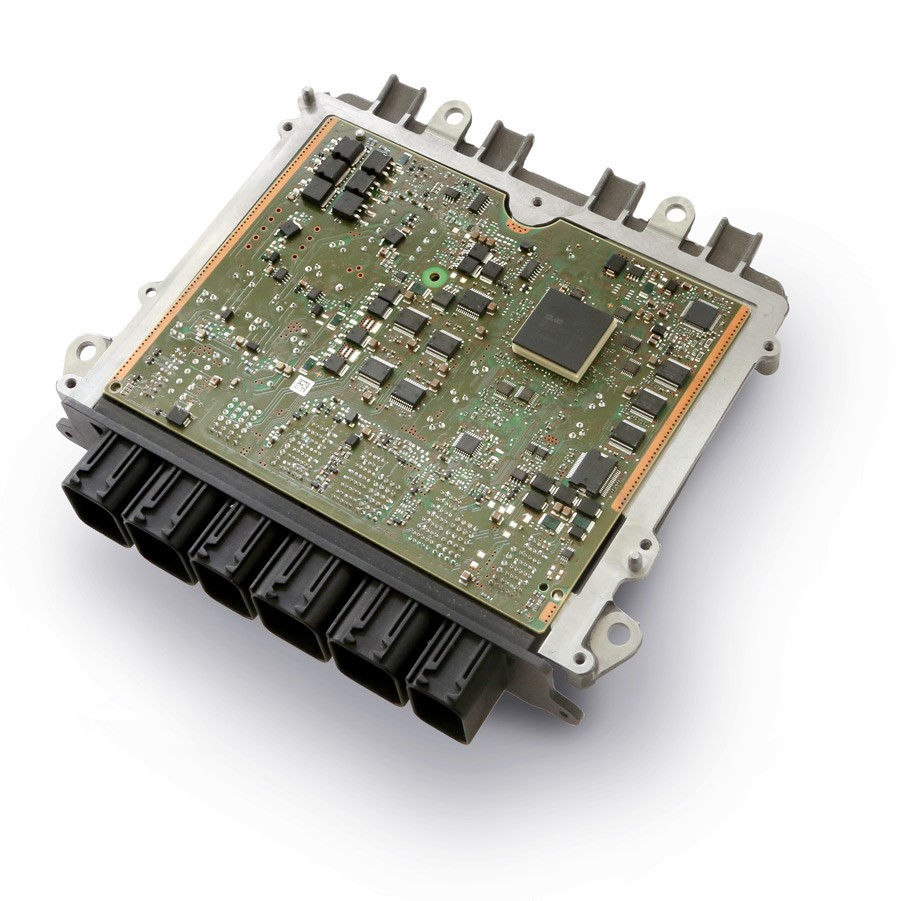
\includegraphics[width=0.5\textwidth]{Kapitel2/Bilder/image13}}
  \caption{Behälter ohne Auslauf als Beispiel für ein System ohne Ausgleich}
  \label{fig:SysohneAusgleich}
\end{figure}

\noindent Die Füllstandshöhe h(t) wird über die Gleichung


\begin{equation}\label{eq:fiftyseven}
x(t)=\frac{1}{A}\cdot\int\limits _{0}^{t}Q(\tau)d\tau+X_{0}
\end{equation}

\noindent beschrieben. Ableiten von Gleichung (\ref{eq:fiftyseven}) führt zu der Differentialgleichung

\begin{equation}\label{eq:fiftyeight}
0\cdot x(t) + \frac{dx}{dt}=\frac{1}{A}\cdot Q(t)
\end{equation}

\noindent Es existiert kein stationäres Gleichgewicht, da im stationären Gleichgewicht die Ableitung dh/dt zu null würde. Gleichung (\ref{eq:fiftyeight}) kann in diesem Fall nicht erfüllt werden, da der Koeffizient $a_{0}=0$ ist. Gleichung (\ref{eq:fiftyseven}) zeigt, dass die Füllstandshöhe h kontinuierlich ansteigt. Das Systemverhalten ist in Bild \ref{fig:Behaelter}  für eine Querschnittsfläche $A=10m^2$ und einen Anfangszustand $x_{0}=2m$ dargestellt.

\begin{figure}[H]
  \centerline{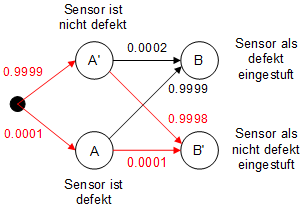
\includegraphics[width=1\textwidth]{Kapitel2/Bilder/image14}}
  \caption{Anregung eines Tanks ohne Auslauf mit einem konstanten Volumenstrom}
  \label{fig:Behaelter}
\end{figure}

\noindent Ein Volumenstrom $Q(t) > 0$ führt zu einem Anstieg der Füllstandshöhe. Es findet kein Ausgleich statt. Es handelt sich demnach um ein System ohne Ausgleich.

\clearpage

\subsubsection{Zusammenfassung grundlegender Systemeigenschaften}

Tabelle \ref{tab:threefour} fasst die diskutierten Systemeigenschaften und ihre Bedeutung zusammen.

\begin{table}[H]
\caption{Zusammenfassung von Systemeigenschaften und ihrer Bedeutung}
\setlength{\fboxsep}{0pt}%
\colorbox{lightgray}{%
\arrayrulecolor{white}%
\begin{tabular}{| c | c |}
\hline
\parbox[c][0.28in][c]{3.3in}{\smallskip\centering\textbf{\fontfamily{phv}\selectfont{Eigenschaft}}} & \parbox[c][0.28in][c]{3.3in}{\smallskip\centering\textbf{\fontfamily{phv}\selectfont{Bedeutung}}}\\ \hline

\parbox[c][1.2in][c]{3.3in}{\centering{\fontfamily{phv}\selectfont{Linearität}}} &
\parbox[c][1.2in][c]{3.3in}{\centering{\fontfamily{phv}\selectfont{System reagiert auf Linearkombination von Eingangssignale  \\
$u(t)=v_{1}\cdot u_{1}(t)+v_{2}\cdot u_{2}(t)$\\
mit derselben Linearkombination von Ausgangssignalen\\
$y(t)=v_{1}\cdot y_{1}(t)+v_{2}\cdot y_{2}(t)$}}}\\ \hline

\parbox[c][0.64in][c]{3.3in}{\centering{\fontfamily{phv}\selectfont{Zeitinvarianz}}} & \parbox[c][0.64in][c]{3.3in}{\centering{\fontfamily{phv}\selectfont{System reagiert auf ein verzögertes\\
Eingangssignal $u(t - t_{0})$\\
mit einem Ausgangsignal $y(t - t_{0})$}}}\\ \hline

\parbox[c][0.64in][c]{3.3in}{\centering{\fontfamily{phv}\selectfont{Kausalität}}} &
\parbox[c][0.64in][c]{3.3in}{\centering{\fontfamily{phv}\selectfont{System reagiert auf ein Eingangssignal\\
erst nach Beginn der Anregung}}}\\ \hline

\parbox[c][0.64in][c]{3.3in}{\centering{\fontfamily{phv}\selectfont{Asymptotische Stabilität}}} & 
\parbox[c][0.64in][c]{3.3in}{\centering{\fontfamily{phv}\selectfont{System erreicht nach einer Anregung\\
mit endlicher Energie\\
wieder seine Ruheposition}}}\\ \hline

\parbox[c][0.64in][c]{3.3in}{\centering{\fontfamily{phv}\selectfont{Grenzstabilität}}} & 
\parbox[c][0.64in][c]{3.3in}{\centering{\fontfamily{phv}\selectfont{System bleibt nach einer Anregung\\
mit endlicher Energie\\
in dem aktuellen Zustand}}}\\ \hline

\parbox[c][0.8in][c]{3.3in}{\centering{\fontfamily{phv}\selectfont{Instabilität}}} & 
\parbox[c][0.8in][c]{3.3in}{\centering{\fontfamily{phv}\selectfont{System reagiert nach einer Anregung mit endlicherEnergie mit einer divergierenden Systemantwort}}}\\ \hline

\parbox[c][0.64in][c]{3.3in}{\centering{\fontfamily{phv}\selectfont{System mit Ausgleich}}} & 
\parbox[c][0.64in][c]{3.3in}{\centering{\fontfamily{phv}\selectfont{Differentialgleichung mit dem Koeffizienten\\
$a_{0}\neq 0$}}}\\ \hline

\end{tabular}%
}
\label{tab:threefour}
\end{table}

\clearpage

\subsection{Lösung linearer Differentialgleichungen mit konstanten Koeffizienten}\label{threethree}
Zur Charakterisierung von Systemen werden oftmals Sprung- und Impulsantworten verwendet. Sie lassen sich bei linearen, zeitinvarianten Systemen im Zeitbereich mit der Vier-Schritt-Methode berechnen.

\subsubsection{Lösung von Anfangswertproblemen mit der Vier-Schritt-Methode}
Bei technischen Anwendungen werden lineare, zeitinvariante Systeme durch lineare Differentialgleichungen mit konstanten Koeffizienten beschrieben.

\begin{equation}\label{eq:fiftynine}
a_{0}\cdot y(t) + a_{1}\cdot \frac{dy}{dt}+a_{2}\cdot \frac{d^2y}{dt^2}+ ... +a_{n}\cdot \frac{d^Ny}{dt^N}=
b_{0}\cdot u(t) + b_{1}\cdot \frac{du}{dt}+b_{2}\cdot \frac{d^2u}{dt^2}+ ... +b_{m}\cdot \frac{d^Mu}{dt^M}
\end{equation}

\noindent Zur Charakterisierung dieser Systeme kann das Einschwingverhalten y(t) unter Berücksichtigung von Anfangswerten des Signals y(t = 0) bestimmt werden. Diese Aufgabenstellungen werden in der Mathematik als Anfangswertprobleme bezeichnet. Die Lösung dieser Anfangswertprobleme erfolgt mit der Vier-Schritt-Methode. Grundlage für das Lösungsverfahren ist, zunächst alle sogenannten homogenen Lösungen der Differentialgleichung zu finden und sie dann mit einer sogenannten partikulären Lösung zu kombinieren. Aus der Menge dieser Lösungen wird abschließend diejenige ausgewählt, die die Anfangsbedingungen der Aufgabenstellung erfüllt. Die Vier-Schritt-Methode umfasst damit folgende Schritte:

\begin{itemize}
  \item Berechnung der allgemeinen homogenen Lösungen
  \item Berechnung einer partikulären Lösung
  \item Superposition von homogener und partikulärer Lösung
  \item Bestimmung der Konstanten über Anfangsbedingungen
\end{itemize}

\noindent Eine ausführliche Darstellung der Vier-Schritt-Methode mit unterschiedlichen Lösungsvarianten ist in [Papu11] und [Goeb11] zu finden. Hier wird eine Lösungsmöglichkeit beschrieben und am Beispiel des RC-Netzwerks angewendet.\bigskip

{\fontfamily{phv}\selectfont
\noindent\textbf{Berechnung der allgemeinen homogenen Lösungen}}\smallskip

\noindent Die lineare Differentialgleichung mit konstanten Koeffizienten (\ref{eq:fiftynine}) beschreibt den Zusammenhang
zwischen Eingangssignal u(t) und Ausgangssignal y(t). Zur Bestimmung der homogenen Differentialgleichungen wird das Eingangssignal u(t) zu null gesetzt.

\begin{equation}\label{eq:sixty}
a_{0}\cdot y_{H}(t) + a_{1}\cdot \frac{dy_{H}}{dt}+a_{2}\cdot \frac{d^2y_{H}}{dt^2}+ ... +a_{n}\cdot \frac{d^Ny_{H}}{dt^N}=
0
\end{equation}

\noindent Die Gleichung besteht aus einer mit den Koeffizienten an gewichteter Summe der Funktion $y_{H}(t)$ und ihren Ableitungen. Zur Lösung dieser Gleichung wird eine Exponentialfunktion angesetzt.

\begin{equation}\label{eq:sixtyone}
y_{H}(t) + Y_{0}\cdot e^{\lambda \cdot t}
\end{equation}

\noindent Sie hat die Eigenschaft, dass ihre Ableitungen selbst wieder Exponentialfunktionen sind.

\begin{equation}\label{eq:sixtytwo}
\frac{d^n y_{H}}{dt^n}= \lambda ^n \cdot e^{\lambda \cdot t}
\end{equation}

\noindent Durch Einsetzen in die homogene Differentialgleichung ergibt sich die Gleichung

\begin{equation}\label{eq:sixtythree}
\begin{split}
0 & = a_{0} \cdot y_{H} \left(t\right)+a_{1} \cdot \frac{dy_{H} }{dt} +a_{2} \cdot \frac{d^{2} y_{H} }{dt^{2} } +...+a_{N} \cdot \frac{d^{N} y_{H} }{dt^{N} }\\ \medskip
& = a_{0} \cdot Y_{0}\cdot e^{\lambda \cdot t} + a_{1}\cdot\lambda \cdot Y_{1}\cdot e^{\lambda \cdot t} + a_{2}\cdot\lambda ^2 \cdot Y_{2}\cdot e^{\lambda \cdot t} +...+ a_{N}\cdot\lambda ^N \cdot Y_{N}\cdot e^{\lambda \cdot t}\\\medskip
& = (a_{0} + a_{1}\cdot\lambda + a_{2}\cdot\lambda ^2 + ... + a_{N}\cdot\lambda ^N) \cdot Y_{0} \cdot e^{\lambda\cdot t}
\end{split}
\end{equation}

\noindent Die Gleichung ist für $Y_{0} = 0$  erfüllt. Dieser Fall ist jedoch technisch weniger von Interesse, da er den Ruhezustand des Systems beschreibt. Für $Y_{0} \neq 0$ kann die Gleichung vereinfacht werden zu

\begin{equation}\label{eq:sixtyfour}
0 = a_{0}+a_{1}\cdot \lambda + a_{2}\cdot \lambda ^2 +...+a_{N}\cdot \lambda ^N
\end{equation}

\noindent Mit der Gleichung werden die Werte $\lambda _{n}$ bestimmt, für die die Exponentialfunktion die vorliegende homogene Differentialgleichung löst. Die Gleichung wird deshalb auch charakteristische Gleichung des Systems genannt. Ein Polynom N-ter Ordnung weist N Nullstellen auf, sodass die Nullstellen
$\lambda _{1} ... \lambda _{N}$ Lösungen der charakteristischen Gleichung sind. Es kann gezeigt werden, dass sich die allgemeine Lösung der homogenen Differentialgleichung $y_{H}(t)$ bei einfachen Nullstellen $\lambda _{n}$ aus der Linearkombination

\begin{equation}\label{eq:sixtyfive}
y_{H} \left(t\right)=Y_{1} \cdot e^{\lambda _{1} \cdot t} +Y_{2} \cdot e^{\lambda _{2} \cdot t} +...+Y_{N} \cdot e^{\lambda _{N} \cdot t} 
\end{equation}

\noindent ergibt [Goeb11]. Die Lösungen der charakteristischen Gleichung müssen jedoch nicht die Vielfachheit von eins haben. Existiert eine P-fache Nullstelle $\lambda _{1}$, ergibt sich die homogene Lösung

\begin{equation}\label{eq:sixtysix}
y_{H} \left(t\right)=Y_{1} \cdot e^{\lambda _{1} \cdot t} +Y_{2} \cdot t\cdot e^{\lambda _{1} \cdot t} +...+Y_{P} \cdot t^{P-1} \cdot e^{\lambda _{1} \cdot t} +Y_{P+1} \cdot e^{\lambda _{2} \cdot t} +Y_{P+2} \cdot e^{\lambda _{3} \cdot t} +...+Y_{N} \cdot e^{\lambda _{N-P+1} \cdot t}
\end{equation}

\noindent
\colorbox{lightgray}{%
\arrayrulecolor{white}%
\renewcommand\arraystretch{0.6}%
\begin{tabular}{ wl{16.5cm} }
{\smallskip{\fontfamily{phv}\selectfont{
Beispiel: Einschwingverhalten eines RC-Netzwerks}}} 
\end{tabular}%
}\bigskip

\noindent Als Beispiel wird das Einschaltverhalten des RC-Netzwerks aus Bild \ref{fig:RCSchaltbild} berechnet. Die Ausgangsspannung des RC-Netzwerks wird über die Differentialgleichung

\begin{equation}\label{eq:sixtyseven}
R \cdot C \cdot\frac{dU_{A}}{dt} + U_{A}(t) =U_{E}(t) 
\end{equation}

\noindent beschrieben. Die zugehörige homogene Differentialgleichung lautet

\begin{equation}\label{eq:sixtyeight}
R \cdot C \cdot\frac{dU_{AH}}{dt} + U_{AH}(t) =0
\end{equation}

\noindent Einsetzen der Exponentialfunktion

\begin{equation}\label{eq:sixtynine}
 u_{AH}(t)= U_{H} \cdot e^{\lambda \cdot t}
\end{equation}

\noindent führt mit $U_{H} \neq 0$ zu der charakteristischen Gleichung

\begin{equation}\label{eq:seventy}
 0=U_{AH}(t)= R \cdot C \cdot \lambda U_{H} \cdot e^{\lambda \cdot t}+U_{H} \cdot e^{\lambda \cdot t}= (R \cdot C \cdot \lambda +1)\cdot U_{H} \cdot e^{\lambda \cdot t}
\end{equation}

\noindent mit der Lösung 

\begin{equation}\label{eq:seventyone}
\lambda=-\frac{1}{R\cdot C}
\end{equation}

\noindent Damit ergibt sich die Lösung der homogenen Differentialgleichung zu

\begin{equation}\label{eq:seventytwo}
u_{AH}(t) = U_{H} \cdot e^{-\frac{1}{R\cdot C}\cdot t}
\end{equation}

\noindent Die Konstante $U_{H}$ ist zunächst unbekannt, sie wird später über die Anfangsbedingungen des Systems bestimmt.\medskip

{\fontfamily{phv}\selectfont
\noindent\textbf{Berechnung einer partikulären Lösung}} \smallskip

\noindent Im zweiten Schritt wird eine partikuläre oder spezielle Lösung der Differentialgleichung bestimmt. Dabei wird von der Differentialgleichung

\begin{equation}\label{eq:seventythree}
a_{0}\cdot y(t) + a_{1}\cdot \frac{dy}{dt}+a_{2}\cdot \frac{d^2y}{dt^2}+ ... +a_{n}\cdot \frac{d^Ny}{dt^N}=
b_{0}\cdot u(t) + b_{1}\cdot \frac{du}{dt}+b_{2}\cdot \frac{d^2u}{dt^2}+ ... +b_{m}\cdot \frac{d^Mu}{dt^M}
\end{equation}

\noindent mit $u(t) \neq 0$ ausgegangen, und es wird für $t\geqslant  0$ eine Lösung gesucht. Wesentlich ist, dass eine beliebige partikuläre Lösung ausreicht, da sie durch Kombination mit der allgemeinen homogenen Lösung das Anfangswertproblem beschreibt.
Eine partikuläre Lösung der Differentialgleichung kann auf verschiedene Arten bestimmt werden [Goeb11]. Hier wird die Lösung durch Lösungsansätze vorgestellt. Die Lösungsansätze sind im Allgemeinen von der Ordnung der Differentialgleichung abhängig und können in [Papu01] oder [Goeb11] nachgeschlagen werden. Für die hier relevanten Fälle einer konstanten Anregung oder einer harmonischen Anregung sind die Lösungsansätze jedoch von der Ordnung der Differentialgleichung unabhängig. Sie sind in Tabelle \ref{tab:threefive} zusammengefasst.

\begin{table}[H]
\caption{Lösungsansätze für die partielle Lösung linearer Differentialgleichungen mit konstanten Koeffizienten}
\setlength{\fboxsep}{0pt}%
\colorbox{lightgray}{%
\arrayrulecolor{white}%
\begin{tabular}{| c | c |}
\hline
\parbox[c][0.28in][c]{3.3in}{\smallskip\centering\textbf{\fontfamily{phv}\selectfont{Eingangssignal u(t) für $t \geqslant 0$}}} & \parbox[c][0.28in][c]{3.3in}{\smallskip\centering\textbf{\fontfamily{phv}\selectfont{Lösungsansatz y$_{p}(t)$}}}\\ \hline

\parbox[c][0.64in][c]{3.3in}{\centering{\fontfamily{phv}\selectfont{Konstantes Eingangssignal\\
u(t) = U}}} &
\parbox[c][0.64in][c]{3.3in}{\centering{\fontfamily{phv}\selectfont{Konstantes Ausgangssignal\\
y$_{P}$(t) = Y}}}\\ \hline

\parbox[c][1in][c]{3.3in}{\centering{\fontfamily{phv}\selectfont{Harmonisches Eingangssignal\\
u(t) = U $\cdot$ cos($\omega t + \mu _{x}$)}}} & \parbox[c][1in][c]{3.3in}{\centering{\fontfamily{phv}\selectfont{Harmonisches Ausgangssignal\\
y$_{P}$(t) = Y $\cdot$ cos($\omega t + \mu _{y}$)\\
wenn $j\cdot\omega$ keine Lösung\\
der charakteristischen Gleichung ist}}}\\ \hline

\parbox[c][1in][c]{3.3in}{\centering{\fontfamily{phv}\selectfont{Exponentielles Eingangssigna\\
u(t) = U $\cdot$ e$^{c\cdot x}$}}} &
\parbox[c][1in][c]{3.3in}{\centering{\fontfamily{phv}\selectfont{Exponentielles Ausgangssignal\\
y$_{P}$(t) = Y$\cdot$ e$^{c\cdot x}$\\
wenn c keine Lösung \\ der charakteristischen Gleichung ist}}}\\ \hline

\end{tabular}%
}
\label{tab:threefive}
\end{table}

\noindent Die freien Parameter des Lösungsansatzes ergeben sich aus dem vorliegenden Eingangssignal sowie
der vorliegenden Differentialgleichung. Dies wird am einfachsten an einem konkreten Beispiel deutlich.\bigskip

\noindent
\colorbox{lightgray}{%
\arrayrulecolor{white}%
\renewcommand\arraystretch{0.6}%
\begin{tabular}{ wl{16.5cm} }
{\fontfamily{phv}\selectfont{
Beispiel: Einschwingverhalten eines RC-Netzwerks}}
\end{tabular}%
}\bigskip

\noindent Zur Berechnung der Systemreaktion auf ein konstantes Eingangssignal der Größe $U_{E0}$ wird für $t \geqslant 0$ das Eingangssignal

\begin{equation}\label{eq:seventyfour}
u_{E} \left(t\right)=U_{E0} 
\end{equation}

\noindent in die Differentialgleichung eingesetzt.

\begin{equation}\label{eq:seventyfive}
R\cdot C\cdot \frac{du_{AP} }{dt} +u_{AP} \left(t\right)=U_{E0} 
\end{equation}

\noindent Der Ansatz für die partikuläre Lösung bei einer konstanten Anregung ist wieder eine Konstante. 

\begin{equation}\label{eq:seventysix}
u_{AP} \left(t\right)=U_{A0}
\end{equation}

\noindent Ihre Ableitung ist null. Einsetzen in die Differentialgleichung führt zu

\begin{equation}\label{eq:seventyseven}
R\cdot C\cdot 0+U_{A0} =U_{E0}
\end{equation}

\noindent Die beiden Konstanten U$_{E0}$ und U$_{A0}$ sind demnach identisch, sodass die partikuläre Lösung für t $\geq$ 0 lautet:

\begin{equation}\label{eq:seventyeight}
u_{AP} \left(t\right)=U_{E0}
\end{equation}

\noindent Das hier vorgestellte Verfahren führt zu einem stetigen Ausgangssignal. Es versagt, wenn das Ausgangssignal Sprünge oder Impulse aufweist. Für die korrekte Berechnung der Systemantwort muss in dem Fall eine sogenannte Übergangsbedingung berücksichtigt werden. Das entsprechende Verfahren wird in Abschnitt 3.3.2 beschrieben..\bigskip

{\fontfamily{phv}\selectfont
\noindent\textbf{Superposition von homogener und partikulärer Lösung}}\smallskip

\noindent Sind die allgemeine homogene Lösung und eine partikuläre Lösung bekannt, ergibt sich die Lösung der Differentialgleichung aus deren Summe.

\begin{equation}\label{eq:seventynine}
y\left(t\right)=y_{H} \left(t\right)+y_{P} \left(t\right)
\end{equation}

\noindent Dabei weist die homogene Lösung noch unbekannte Parameter auf, die später über Anfangsbedingungen
zu bestimmen sind.\bigskip

\noindent
\colorbox{lightgray}{%
\arrayrulecolor{white}%
\renewcommand\arraystretch{0.6}%
\begin{tabular}{ wl{16.5cm} }
{\fontfamily{phv}\selectfont{
Beispiel: Einschwingverhalten eines RC-Netzwerks}}
\end{tabular}%
}\bigskip

\noindent Bei dem Einschaltverhalten eines RC-Netzwerks ergibt sich die Lösung aus der Summe von homogener Lösung

\begin{equation}\label{eq:eighty}
u_{AH} \left(t\right)=U_{H} \cdot e^{-\frac{1}{R\cdot C} \cdot t}
\end{equation}

\noindent und partikulärer Lösung

\begin{equation}\label{eq:eightyone}
u_{AP} \left(t\right)=U_{E0} 
\end{equation}

\noindent zu

\begin{equation}\label{eq:eightytwo}
u_{A} \left(t\right)=U_{H} \cdot e^{-\frac{1}{R\cdot C} \cdot t} +U_{E0}
\end{equation}

\noindent Dabei ist die Konstante U$_{H}$ noch unbekannt.\bigskip

{\fontfamily{phv}\selectfont
\noindent\textbf{Bestimmung der Konstanten über Anfangsbedingungen}}\smallskip

\noindent Die Summe aus homogener und partikulärer Lösung weist Parameter auf, die bestimmt werden müssen. Es kann gezeigt werden, dass bei einer Differentialgleichung N-ter Ordnung N Parameter zu bestimmen sind. Dazu werden N Bedingungen benötigt. Bei Anfangswertproblemen sind diese Bedingungen
die Anfangswerte der Funktion y(t) und ihrer N - 1 Ableitungen an der Stelle t = 0.\bigskip

\noindent
\colorbox{lightgray}{%
\arrayrulecolor{white}%
\renewcommand\arraystretch{0.6}%
\begin{tabular}{ wl{16.5cm} }
{\fontfamily{phv}\selectfont{
Beispiel: Einschwingverhalten eines RC-Netzwerks}}
\end{tabular}%
}\bigskip

\noindent Bei dem RC-Netzwerk handelt es sich um ein System, das mit einer Differentialgleichung erster Ordnung beschrieben wird. Die allgemeine Lösung lautet

\begin{equation}\label{eq:eightythree}
u_{A} \left(t\right)=U_{H} \cdot e^{-\frac{1}{R\cdot C} \cdot t} +U_{E0}
\end{equation}

\noindent Zur Bestimmung des Parameters U${}_{H}$ wird die Ausgangsspannung u${}_{A}$(0) verwendet. Es ergibt sich

\begin{equation}\label{eq:eightyfour}
u_{A} \left(0\right)=U_{H} \cdot e^{-\frac{1}{R\cdot C} \cdot 0} +U_{E0} =U_{H} +U_{E0}
\end{equation}

\noindent beziehungsweise

\begin{equation}\label{eq:eightyfive}
U_{H} =u_{A} \left(0\right)-U_{E0}
\end{equation}

\noindent Daraus ergibt sich die Lösung des Anfangswertproblems in Abhängigkeit der Ausgangsspannung u$_{A}$(0) zum Zeitpunkt t = 0 zu

\begin{equation}\label{eq:eightysix}
u_{A} \left(t\right)=\left(u_{A} \left(0\right)-U_{E0} \right)\cdot e^{-\frac{1}{R\cdot C} \cdot t} +U_{E0} =u_{A} \left(0\right)\cdot e^{-\frac{1}{R\cdot C} \cdot t} +U_{E0} \cdot \left(1-e^{-\frac{1}{R\cdot C} \cdot t} \right)
\end{equation}

\noindent Die Ausgangsspannung setzt sich aus zwei Termen zusammen. Der erste Term beschreibt das Abklingen der Anfangsbedingung, der zweite Term beschreibt die Reaktion des Systems auf einen Spannungssprung am Eingang. Bild \ref{fig:RCEinschwingenAnfangsbedingungen} zeigt das Einschwingverhalten der Kondensatorspannung u$_{A}$(t) für eine Spannung U$_{E0}$ = 5 V, einen Widerstand von 5 k$\Omega$ und eine Kapazität von 4 nF bei unterschiedlichen
Anfangswerten.

\begin{figure}[H]
  \centerline{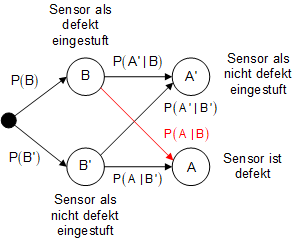
\includegraphics[width=0.5\textwidth]{Kapitel2/Bilder/image15}}
  \caption{Einschwingverhalten der Kondensator Spannung u${}_{A}$(t) bei Anregung mit einem Spannungssprung von 5 V und verschiedenen Anfangsbedingungen u${}_{A}$(0)}
  \label{fig:RCEinschwingenAnfangsbedingungen}
\end{figure}

\noindent Das Ausgangssignal schwingt abhängig von dem Anfangswert auf den Endwert von u$_{A}$ = 5 V ein.\bigskip
\clearpage

{\fontfamily{phv}\selectfont
\noindent\textbf{Zusammenfassung}}\smallskip

\noindent Das Vorgehen bei der Vierschrittmethode zur Lösung linearer Differentialgleichungen mit konstanten Koeffizienten ist in Tabelle \ref{tab:threesix} zusammengefasst.

\begin{table}[H]
\caption{Lösungsansätze für die partielle Lösung linearer Differentialgleichungen mit konstanten Koeffizienten}
\setlength{\fboxsep}{0pt}%
\colorbox{lightgray}{%
\arrayrulecolor{white}%
\begin{tabular}{| c | c |}
\hline
\parbox[c][0.28in][c]{0.45in}{\smallskip\centering\textbf{\fontfamily{phv}\selectfont{Schritt}}} & \parbox[c][0.28in][c]{6in}{\smallskip\centering\textbf{\fontfamily{phv}\selectfont{Beschreibung}}}\\ \hline

\parbox[c][2in][c]{0.45in}{\centering{1}} &
\parbox[c][2in][c]{6in}{\centering{\fontfamily{phv}\selectfont{
Lösung der homogenen Differentialgleichung\\
$a_{0} \cdot y_{H} \left(t\right)+a_{1} \cdot \frac{dy_{H} }{dt} +a_{2} \cdot \frac{d^{2} y_{H} }{dt^{2} } +...+a_{N} \cdot \frac{d^{N} y_{H} }{dt^{N} } =0$ \\ 
über Ansatz\\
$y_{H} \left(t\right)=Y_{0} \cdot e^{\lambda \cdot t} $\newline 
durch Lösen der charakteristischen Gleichung\\
$0=a_{0} +a_{1} \cdot \lambda +a_{2} \cdot \lambda ^{2} +...+a_{N} \cdot \lambda ^{N} $\\
Allgemeine Lösung in Abhängigkeit der Vielfachheit\\ 
$y_{H} \left(t\right)=Y_{1} \cdot e^{\lambda _{1} \cdot t} +Y_{2} \cdot t\cdot e^{\lambda _{1} \cdot t} +...+Y_{P} \cdot t^{P-1} \cdot e^{\lambda _{1} \cdot t} +Y_{P+1} \cdot e^{\lambda _{2} \cdot t} +Y_{P+2} \cdot e^{\lambda _{3} \cdot t} +...+Y_{N} \cdot e^{\lambda _{N-P+1} \cdot t} $

}}}\\ \hline

\parbox[c][0.5in][c]{0.45in}{\centering{2}} & \parbox[c][0.5in][c]{6in}{\centering{\fontfamily{phv}\selectfont{Bestimmung einer partikulären Lösung y${}_{p}$(t) über einen Lösungsansatz je nach Eingangssignal}}}\\ \hline

\parbox[c][0.5in][c]{0.45in}{\centering{3}} &
\parbox[c][0.5in][c]{6in}{\centering {\fontfamily{phv}\selectfont{Superposition von allgemeiner homogener und partikulärer Lösung\\ 
$y\left(t\right)=y_{H} \left(t\right)+y_{P} \left(t\right)$}}}\\ \hline

\parbox[c][0.4in][c]{0.45in}{\centering{4}} &
\parbox[c][0.4in][c]{6in}{\centering{\fontfamily{phv}\selectfont{Bestimmung der unbekannten Konstanten über Anfangsbedingungen}}}\\ \hline

\end{tabular}%
}\bigskip
\label{tab:threesix}
\end{table}

\subsubsection{Exkurs zu Übergangsbedingungen bei linearen Differentialgleichungen}\label{threethreetwo}

\noindent Die in Abschnitt 3.3.1 beschriebene Vier-Schritt-Methode eignet sich zur Lösung linearer Differentialgleichung, bei denen das Ausgangssignal stetig ist. Deshalb wird die Vier-Schritt-Methode stufenweise ergänzt, um Sprünge oder allgemein Singularitäten berücksichtigen zu können.\bigskip

{\fontfamily{phv}\selectfont
\noindent\textbf{Lösung linearer Differentialgleichungen bei stetigem Ausgangssignal (N $\boldsymbol{\mathrm{>}}$ P)}}

\noindent Ist das Ausgangssignal stetig, sind rechter und linker Grenzwert an der Stelle t = 0 identisch.

\begin{equation}\label{eq:eightyseven}
y\left(0_{+} \right)=y\left(0_{-} \right)
\end{equation}

\noindent Die Rechnung erfolgt in diesem Fall wie in Abschnitt 3.3.1. Zur Überleitung wird dieser Fall noch einmal aufgegriffen und hinsichtlich der Anfangsbedingung intensiver interpretiert.\bigskip

\noindent
\colorbox{lightgray}{%
\arrayrulecolor{white}%
\renewcommand\arraystretch{0.6}%
\begin{tabular}{ wl{16.5cm} }
{\fontfamily{phv}\selectfont{
Beispiel: Lineare Differentialgleichung und stetiges Ausgangssignal}}
\end{tabular}%
}\bigskip

\noindent Als einführendes Beispiel wird das Ausgangssignal für ein System mit der Differentialgleichung

\begin{equation}\label{eq:eightyeight}
\frac{dy}{dt} +6\cdot y\left(t\right)=u\left(t\right)
\end{equation}

\noindent berechnet. Das Eingangssignal ist 

\begin{equation}\label{eq:eightynine}
\frac{dy}{dt} +6\cdot y\left(t\right)=u\left(t\right)
\end{equation}

\noindent und die Anfangsbedingung lautet y(0${}_{-}$) = U${}_{1}$. Zur Berechnung des Ausgangssignals y(t) wird zunächst für t $\mathrm{>}$ 0 die homogene Differentialgleichung 

\begin{equation}\label{eq:ninety}
\frac{dy_{H} }{dt} +6\cdot y_{H} \left(t\right)=0
\end{equation}

\noindent mit dem Ansatz

\begin{equation}\label{eq:ninetyone}
y_{H} \left(t\right)=Y_{H} \cdot e^{\lambda \cdot t} \cdot \sigma \left(t\right)
\end{equation}

\noindent gelöst. Für t $\mathrm{>}$ 0 ergibt sich über durch Einsetzen 

\begin{equation}\label{eq:ninetytwo}
\lambda \cdot Y_{H} \cdot e^{\lambda \cdot t} +6\cdot Y_{H} \cdot e^{\lambda \cdot t} =0
\end{equation}

\noindent die charakteristische Gleichung

\begin{equation}\label{eq:ninetythree}
\lambda +6=0
\end{equation}

\noindent Sie besitzt die Lösung $\lambda$ = - 6. Damit lautet für t $\mathrm{>}$ 0 die allgemeine homogene Lösung

\begin{equation}\label{eq:ninetyfour}
y_{H} \left(t\right)=Y_{H} \cdot e^{-6\cdot t} \cdot \sigma \left(t\right)
\end{equation}

\noindent Da das Eingangssignal für t $\mathrm{>}$ 0 konstant ist, ist die Konstante y${}_{P}$(t) = Y${}_{P}$ eine partikuläre Lösung. Einsetzen in die Differentialgleichung führt zu

\begin{equation}\label{eq:ninetyfive}
0+6\cdot Y_{P} =U_{0} 
\end{equation}

\noindent beziehungsweise

\begin{equation}\label{eq:ninetysix}
Y_{P} =\frac{1}{6} \cdot U_{0}
\end{equation}

\noindent Damit lautet die L\"{o}sung der Differentialgleichung

\begin{equation}\label{eq:ninetyseven}
y\left(t\right)=y_{H} \left(t\right)+y_{P} \left(t\right)=\left(Y_{H} \cdot e^{-6\cdot t} +\frac{1}{6} \cdot U_{0} \right)\cdot \sigma \left(t\right)
\end{equation}

\noindent Das Eingangssignal u(t) ist an der Stelle t = 0 nicht stetig, es springt. Um die Differentialgleichung 

\begin{equation}\label{eq:ninetyeight}
\frac{dy}{dt} +6\cdot y\left(t\right)=u\left(t\right)
\end{equation}

\noindent erfüllen zu können, muss auch das Ausgangssignal y(t) oder eine Ableitung des Ausgangssignals springen. $\frac{dy}{dt} +6\cdot y\left(t\right)=u\left(t\right)$W\"{u}rde y(t) springen, wäre dy/dt ein Impuls. Dieser Impuls hat kein entsprechendes Pendant auf der Eingangsseite. Deshalb muss dy/dt an der Stelle t = 0 springen. Das Signal y(t) ist damit an der Stelle t = 0 stetig und springt nicht. 

\begin{equation}\label{eq:ninetynine}
y\left(0_{+} \right)=y\left(0_{-} \right)=U_{1}
\end{equation}

\noindent Mit diesen Anfangswerten wird die Unbekannte Y${}_{H}$ bestimmt. 

\begin{equation}\label{eq:hundred}
y\left(0_{+} \right)=Y_{H} +\frac{1}{6} \cdot U_{0} =U_{1} 
\end{equation}

\noindent Die Konstante Y${}_{H}$ errechnet sich zu

\begin{equation}\label{eq:hundredone}
Y_{H} =U_{1} -\frac{1}{6} \cdot U_{0} 
\end{equation}

\noindent Damit lautet die Lösung der Differentialgleichung für t $\mathrm{>}$ 0 

\begin{equation}\label{eq:hundredtwo}
y\left(t\right)=\left(\left(U_{1} -\frac{1}{6} \cdot U_{0} \right)\cdot e^{-6\cdot t} +\frac{1}{6} \cdot U_{0} \right)\cdot \sigma \left(t\right)
\end{equation}

\noindent Liegt bei dem Eingangssignal u(t) ein Sprung an der Stelle t = 0 vor, führt diese Unstetigkeit in Kombination mit einer Ableitung du/dt des Eingangssignals zu einem Impuls an der Stelle t = 0. Damit kann die Aufgabenstellung mit der in Abschnitt 3.3.1 beschriebenen Vier-Schritt-Methode alleine nicht gelöst werden. Auch bei höheren Ableitungen des Eingangssignals u(t) in Kombination mit unstetigen Eingangssignalen versagt die Vier-Schritt-Methode. Ein impulsförmiges Eingangssignal u(t) = $\delta$(t) führt ebenfalls zu einer Aufgabenstellung, die mit der Vier-Schritt-Methode alleine nicht gelöst werden kann. 

\begin{equation}\label{eq:hundredthree}
\frac{d\delta }{dt} =\frac{d^{2} \sigma }{dt^{2} }
\end{equation}

\noindent die Ordnung P = 2 auf. Um eine Differentialgleichung für Eingangssignale mit Singularitäten zu lösen, müssen auf beiden Seiten der Differentialgleichung alle Ordnungen der Singularitäten dasselbe Gewicht haben. $a_{n} \cdot \frac{d^{n} y}{dt^{n} } =\sum _{m=0}^{M}b_{m} \cdot \frac{d^{m} u}{dt^{m} }  $In dem Beispiel oben hat diese Abschätzung dazu geführt, dass das Ausgangssignal y(t) stetig ist. Auch bei der Differentialgleichung 

\begin{equation}\label{eq:hundredfour}
\frac{d^{2} y}{dt^{2} } +5\cdot \frac{dy}{dt} +6\cdot y\left(t\right)=\frac{du}{dt}
\end{equation}

\noindent und einem Eingangssignal 

\begin{equation}\label{eq:hundredfive}
u\left(t\right)=U_{0} \cdot \sigma \left(t\right)
\end{equation}

\noindent wäre das Ausgangssignal stetig. Das Eingangssignal weist unter Berücksichtigung der Ableitung eine Singularität der Ordnung P = 1 auf. Deshalb muss die zweite Ableitung von y(t) einen Impuls aufweisen und die erste Ableitung einen Sprung besitzen. Damit ist y(t) stetig. Dieser Ansatz führt deshalb immer dann zum Ergebnis, wenn die Ordnung N der Differentialgleichung grö{\ss}er ist als die Ordnung P der Singularit\"{a}t.

\begin{equation}\label{eq:hundredsix}
N>P
\end{equation}\medskip

{\fontfamily{phv}\selectfont
\noindent\textbf{Lösung linearer Differentialgleichungen bei springendem Ausgangssignal (N = P)}}

\noindent Sind die Ordnungen der Differentialgleichung N und der Singularität P gleich gro{\ss}, weist das Ausgangssignal einen Sprung auf. Die Anfangsbedingung y(0-) ist deshalb nicht identisch zu y(0+) und kann nicht zur Bestimmung der Konstante in der homogenen Lösung verwendet werden. Zur Lösung dieser Aufgabenstellungen wird deshalb eine Übergangsbedingung benötigt, die das Verhalten an der Stelle t = 0 beschreibt. Dazu wird die Lösung y(t) in einen linken Bereich (t $\mathrm{<}$ 0) und einen rechten Bereich (t $\mathrm{>}$ 0) aufgeteilt. 

\begin{equation}\label{eq:hundredseven}
y\left(t\right)=y_{L} \left(t\right)\cdot \sigma \left(-t\right)+y_{R} \left(t\right)\cdot \sigma \left(t\right)
\end{equation}

\noindent Zwischen den beiden Bereichen findet der Sprung des Ausgangsignals statt, der mit Hilfe der Ausblendeigenschaft der Impulsfunktion bestimmt wird. Das Vorgehen wird wieder an einem Beispiel beschrieben.\bigskip

\noindent
\colorbox{lightgray}{%
\arrayrulecolor{white}%
\renewcommand\arraystretch{0.6}%
\begin{tabular}{ wl{16.5cm} }
{\fontfamily{phv}\selectfont{
Beispiel: Lineare Differentialgleichung und stetiges Ausgangssignal}}
\end{tabular}%
}\bigskip

\noindent Um zu untersuchen, wie Differentialgleichungen mit springendem Ausgangssignal berechnet werden, wird die Differentialgleichung

\begin{equation}\label{eq:hundredeight}
\frac{dy}{dt} +6\cdot y\left(t\right)=\frac{du}{dt}
\end{equation}

\noindent bei einem Eingangssignal 

\begin{equation}\label{eq:hundrednine}
u\left(t\right)=U_{0} \cdot \sigma \left(t\right)
\end{equation}

\noindent und der Anfangsbedingung y(0${}_{-}$) = U${}_{1}$ betrachtet. Auf der rechten Seite wird der Sprung am Eingang abgeleitet, es liegt also eine Singularit\"{a}t erster Ordnung (P = 1) vor. Die h\"{o}chste Ableitung auf der linken Seite ist die erste Ableitung des Ausgangssignals (N =1). Um der Singularit\"{a}t auf der rechten Seite zu entsprechen, muss das Ausgangssignal y(t) einen Sprung aufweisen. Es gibt f\"{u}r das Ausgangssignal also eine L\"{o}sung y${}_{R}$(t) f\"{u}r t $\mathrm{>}$ 0 und eine L\"{o}sung y${}_{L}$(t) f\"{u}r t $\mathrm{<}$ 0. 

\begin{equation}\label{eq:hundredten}
y\left(t\right)=y_{L} \left(t\right)\cdot \sigma \left(-t\right)+y_{R} \left(t\right)\cdot \sigma \left(t\right)
\end{equation}

\noindent Formell berechnet sich die erste Ableitung zu

\begin{equation}\label{eq:hundredeleven}
\begin{split}
\frac{dy}{dt}  & = -y_{L} \left(t\right)\cdot \delta \left(-t\right)+\frac{dy_{L} }{dt} \cdot \sigma \left(-t\right)+y_{R} \left(t\right)\cdot \delta \left(t\right)+\frac{dy_{R} }{dt} \cdot \sigma \left(t\right) \\ 
& = \frac{dy_{R} }{dt} \cdot \sigma \left(t\right)+\frac{dy_{L} }{dt} \cdot \sigma \left(-t\right)+\left(y_{R} \left(t\right)-y_{L} \left(t\right)\right)\cdot \delta \left(t\right)  
\end{split}
\end{equation}

\noindent Einsetzen in die Differentialgleichung führt zu

\begin{equation}\label{eq:hundredtwelve}
\frac{dy_{R} }{dt} \cdot \sigma \left(t\right)+\frac{dy_{L} }{dt} \cdot \sigma \left(-t\right)+\left(y_{R} \left(t\right)-y_{L} \left(t\right)\right)\cdot \delta \left(t\right)+6\cdot \left(y_{L} \left(t\right)\cdot \sigma \left(-t\right)+y_{R} \left(t\right)\cdot \sigma \left(t\right)\right)=\frac{du}{dt}
\end{equation}

\noindent F\"{u}r die \"{U}bergangsbedingung ist nur das Verhalten an der Stelle t = 0 relevant. Zur Berechnung der \"{U}bergangsbedingung wird davon ausgegangen, dass die L\"{o}sungen f\"{u}r t $\mathrm{<}$ 0 und t $\mathrm{>}$ 0 existieren.

\begin{equation}\label{eq:hundredthirteen}
\frac{dy_{L} }{dt} +6\cdot y_{L} \left(t\right)=0
\end{equation}

\begin{equation}\label{eq:hundredfourteen}
\frac{dy_{R} }{dt} +6\cdot y_{R} \left(t\right)=0
\end{equation}

\noindent Damit kann Gleichung \eqref{eq:hundredtwelve} vereinfacht werden zu

\begin{equation}\label{eq:hundredfifteen}
\left(y_{R} \left(t\right)-y_{L} \left(t\right)\right)\cdot \delta \left(t\right)=\frac{du}{dt} =U_{0} \cdot \delta \left(t\right)
\end{equation}

\noindent Integrieren der Gleichung 

\begin{equation}\label{eq:hundredsixteen}
\int\limits _{-\infty }^{\infty }\left(y_{R} \left(t\right)-y_{L} \left(t\right)\right)\cdot \delta \left(t\right)\, \, dt =\int\limits _{-\infty }^{\infty }U_{0} \cdot \delta \left(t\right)\, \, dt
\end{equation}

\noindent f\"{u}hrt mit der Ausblendeigenschaft der Impulsfunktion zu 

\begin{equation}\label{eq:hundredseventeen}
y_{R} \left(0\right)-y_{L} \left(0\right)=U_{0}
\end{equation}

\noindent Damit lautet der rechtseitige Anfangswert 

\begin{equation}\label{eq:hundredeighteen}
y\left(0_{+} \right)=y_{R} \left(0\right)=U_{0} +y_{L} \left(0\right)=U_{0} +y\left(0_{-} \right)=U_{0} +U_{1} 
\end{equation}

\noindent An der L\"{o}sung der homogenen Differentialgleichung f\"{u}r t $\mathrm{>}$ 0 \"{a}ndert sich nichts.

\begin{equation}\label{eq:hundrednineteen}
y_{H} \left(t\right)=Y_{H} \cdot e^{-6\cdot t} \cdot \sigma \left(t\right)
\end{equation}

\noindent Da das Eingangssignal u${}_{E}$(t) = U${}_{0}$ f\"{u}r t $\mathrm{>}$ 0 konstant ist, ist die Ableitung null und y${}_{P}$(t) = 0 ist eine partikul\"{a}re L\"{o}sung. Damit lautet die L\"{o}sung der Differentialgleichung

\begin{equation}\label{eq:hundredtwenty}
y\left(t\right)=y_{H} \left(t\right)+y_{P} \left(t\right)=Y_{H} \cdot e^{-6\cdot t} \cdot \sigma \left(t\right)+0=Y_{H} \cdot e^{-6\cdot t} \cdot \sigma \left(t\right)
\end{equation}

\noindent Die Konstante Y${}_{H}$ wird \"{u}ber den berechneten Anfangswert bestimmt 

\begin{equation}\label{eq:hundredtwentyone}
Y_{H} =y\left(0_{+} \right)=U_{0} +U_{1}
\end{equation}

\noindent und die L\"{o}sung der Differentialgleichung lautet 

\begin{equation}\label{eq:hundredtwentytwo}
y\left(t\right)=\left(U_{0} +U_{1} \right)\cdot e^{-6\cdot t} \cdot \sigma \left(t\right)
\end{equation}

\noindent Sie springt erwartungsgem\"{a}{\ss} an der Stelle t = 0. \bigskip

{\fontfamily{phv}\selectfont
\noindent\textbf{Lösung linearer Differentialgleichungen mit impulsförmigen Ausgangssignal (N $\boldsymbol{\mathrm{<}}$ P)}}

\noindent Ist die Ordnung der Differentialgleichung N kleiner als die Ordnung der Singularit\"{a}t P, kann das Ausgangssignal einen Impuls und Ableitungen davon aufweisen. Wie bei dem Beispiel mit N = P muss die Anfangsbedingung y(0${}_{-}$) nicht identisch zu y(0${}_{+}$) sein. Zus\"{a}tzlich sind bei der L\"{o}sung ein Impuls an der Stelle t = 0 und seine Ableitungen mit unbekanntem Gewicht zu ber\"{u}cksichtigen. Je h\"{o}her die Differenz der Singularit\"{a}t P im Vergleich zur Ordnung der Differentialgleichung ist, desto h\"{o}here Ableitungen der Impulse sind zu ber\"{u}cksichtigen. Im Allgemeinen lautet damit die L\"{o}sung der Differentialgleichung

\begin{equation}\label{eq:hundredtwentythree}
y\left(t\right)=y_{L} \left(t\right)\cdot \sigma \left(-t\right)+y_{R} \left(t\right)\cdot \sigma \left(t\right)+\sum _{p=0}^{P-N-1}Y_{p} \cdot \frac{d^{p} \delta }{dt^{p}} 
\end{equation}

\noindent Zur Bestimmung der Hilfe der Gewichte Yp und der Sprungh\"{o}he an der Stelle t = 0 wird auf Eigenschaften der Impulsfunktion zur\"{u}ckgegriffen, wie das folgende Beispiel zeigt.\bigskip

\noindent
\colorbox{lightgray}{%
\arrayrulecolor{white}%
\renewcommand\arraystretch{0.6}%
\begin{tabular}{ wl{16.5cm} }
{\fontfamily{phv}\selectfont{
Beispiel: Lineare Differentialgleichung und stetiges Ausgangssignal}}
\end{tabular}%
}\bigskip

\noindent Ausgangspunkt ist wie bei den Beispielen oben eine Differentialgleichung erster Ordnung.

\begin{equation}\label{eq:hundredtwentyfour}
\frac{dy}{dt} +6\cdot y\left(t\right)=\frac{du}{dt}
\end{equation}

\noindent Das Eingangssignal ist in diesem Beispiel

\begin{equation}\label{eq:hundredtwentyfive}
u\left(t\right)=U_{0} \cdot \delta \left(t\right)
\end{equation}

\noindent und die Anfangsbedingung ist wieder y(0${}_{-}$) = U${}_{1}$. 

\noindent Auf der rechten Seite wird der Impuls am Eingang abgeleitet, es liegt also eine Singularit\"{a}t zweiter Ordnung (P = 2) vor. Die h\"{o}chste Ableitung auf der linken Seite ist die erste Ableitung des Ausgangssignals (N =1). Um der Singularit\"{a}t auf der rechten Seite zu entsprechen, muss das Ausgangssignal y(t) einen Impuls aufweisen. Das Ausgangssignal setzt sich nach Gleichung \eqref{eq:hundredtwentythree} damit zusammen aus einer L\"{o}sung y${}_{R}$(t) f\"{u}r t $\mathrm{>}$ 0, einer L\"{o}sung y${}_{L}$(t) f\"{u}r t $\mathrm{<}$ 0 und einem Impuls mit unbekanntem Gewicht an der Stelle t = 0.

\begin{equation}\label{eq:threehundredtwentysix}
y\left(t\right)=y_{L} \left(t\right)\cdot \sigma \left(-t\right)+y_{R} \left(t\right)\cdot \sigma \left(t\right)+Y_{0} \cdot \delta \left(t\right)
\end{equation}

\noindent Formell berechnet sich die erste Ableitung zu

\begin{equation}\label{eq:threehundredtwentyseven}
\begin{split}
\frac{dy}{dt}  & = -y_{L} \left(t\right)\cdot \delta \left(-t\right)+\frac{dy_{L} }{dt} \cdot \sigma \left(-t\right)+y_{R} \left(t\right)\cdot \delta \left(t\right)+\frac{dy_{R} }{dt} \cdot \sigma \left(t\right)+Y_{0} \cdot \frac{d\delta }{dt}\\ 
& = \frac{dy_{R} }{dt} \cdot \sigma \left(t\right)+\frac{dy_{L} }{dt} \cdot \sigma \left(-t\right)+\left(y_{R} \left(t\right)-y_{L} \left(t\right)\right)\cdot \delta \left(t\right)+Y_{0} \cdot \frac{d\delta }{dt}
\end{split}
\end{equation}

\noindent Einsetzen in die Differentialgleichung f\"{u}hrt zu

\begin{equation}\label{eq:threehundredtwentyeight}
\begin{split}
\frac{du}{dt} & = \frac{dy_{R} }{dt} \cdot \sigma \left(t\right)+\frac{dy_{L} }{dt} \cdot \sigma \left(-t\right)+\left(y_{R} \left(t\right)-y_{L} \left(t\right)\right)\cdot \delta \left(t\right)+Y_{0} \cdot \frac{d\delta }{dt}\\ 
& +6\cdot \left(y_{L} \left(t\right)\cdot \sigma \left(-t\right)+y_{R} \left(t\right)\cdot \sigma \left(t\right)+Y_{0} \cdot \delta \left(t\right)\right)
\end{split}
\end{equation}

\noindent F\"{u}r die \"{U}bergangsbedingung ist nur das Verhalten an der Stelle t = 0 relevant. Wieder wird davon ausgegangen, dass die L\"{o}sungen f\"{u}r t $\mathrm{<}$ 0 und t $\mathrm{>}$ 0 existieren. 

\begin{equation}\label{eq:threehundredtwentynine}
\frac{dy_{L} }{dt} +6\cdot y_{L} \left(t\right)=0
\end{equation}

\begin{equation}\label{eq:threehundredthirty}
\frac{dy_{R} }{dt} +6\cdot y_{R} \left(t\right)=0
\end{equation}

\noindent Damit kann Gleichung \eqref{eq:threehundredtwentyeight} vereinfacht werden zu

\begin{equation}\label{eq:hundredthirtyone}
\left(y_{R} \left(t\right)-y_{L} \left(t\right)\right)\cdot \delta \left(t\right)+Y_{0} \cdot \frac{d\delta }{dt} +6\cdot Y_{0} \cdot \delta \left(t\right)=\frac{du}{dt} =U_{0} \cdot \frac{d\delta }{dt}
\end{equation}

\noindent Da in der Gleichung sowohl ein Impuls als auch seine Ableitung vorkommt, kann die Ausblendeigenschaft nicht alleine zur Aufl\"{o}sung genutzt werden Stattdessen wird die Gleichung \eqref{eq:hundredthirtyone} mit einer Funktion f(t) multipliziert und integriert. 

\begin{equation}\label{eq:threehundredthirtytwo}
\int\limits _{0_{-} }^{0_{+} }\left(\left(y_{R} \left(t\right)-y_{L} \left(t\right)\right)\cdot \delta \left(t\right)+Y_{0} \cdot \frac{d\delta }{dt} +6\cdot Y_{0} \cdot \delta \left(t\right)\right)\cdot f\left(t\right)\, \, dt =\int\limits  _{0_{-} }^{0_{+} }U_{0} \cdot \frac{d\delta }{dt} \cdot f\left(t\right)\, \, dt 
\end{equation}

\noindent Mit Hilfe der partiellen Integration kann das Integral \"{u}ber die Ableitung der Impulsfunktion umgerechnet werden. 

\begin{equation}\label{eq:threehundredthirtythree}
\int\limits  _{0_{-} }^{0_{+} }\frac{d\delta }{dt} \cdot x\left(t\right)\, \, dt =\delta \left(0_{+} \right)\cdot x\left(0_{+} \right)-\delta \left(0_{-} \right)\cdot x\left(0_{-} \right)-\int\limits  _{0_{-} }^{0_{+} }\delta \left(t\right)\cdot \frac{dx}{dt} \, \, dt
\end{equation}

\noindent Da die Impulsfunktion nur an der Stelle t = 0 von null verschieden ist, gilt mit der Ausblendeigenschaft der Impulsfunktion

\begin{equation}\label{eq:threehundredthirtyfour}
\int\limits _{0_{-} }^{0_{+} }\frac{d\delta }{dt} \cdot x\left(t\right)\, \, dt =-\left. \frac{dx}{dt} \right|_{t=0}
\end{equation}

\noindent Wird dieses Verfahren in Kombination mit der Ausblendeigenschaft auf Gleichung \eqref{eq:threehundredthirtyfive} angewendet, ergibt sich

\begin{equation}\label{eq:threehundredthirtyfive}
\left(y_{R} \left(0\right)-y_{L} \left(0\right)\right)\cdot f\left(0\right)-Y_{0} \cdot \left. \frac{df}{dt} \right|_{t=0} +6\cdot Y_{0} \cdot f\left(0\right)=-U_{0} \cdot \left. \frac{df}{dt} \right|_{t=0}
\end{equation}

\noindent Um diese Gleichung f\"{u}r beliebige Funktion f(t) zu erf\"{u}llen, m\"{u}ssen die Koeffizienten von f(0) und df/dt an der Stelle t = 0 \"{u}bereinstimmen. Es ergeben sich als zwei Gleichungen f\"{u}r zwei Unbekannte.

\begin{equation}\label{eq:threehundredthirtysix}
\left(y_{R} \left(0\right)-y_{L} \left(0\right)\right)+6\cdot Y_{0} =0
\end{equation}

\begin{equation}\label{eq:threehundredthirtyseven}
-Y_{0} =-U_{0}
\end{equation}

\noindent Damit ist Y${}_{0}$ = U${}_{0}$ und de Angangswert y(0${}_{+}$) berechnet sich zu

\begin{equation}\label{eq:threehundredthirtyeight}
y\left(0_{+} \right)=y_{R} \left(0\right)=y_{L} \left(0\right)-6\cdot Y_{0} =y\left(0_{-} \right)-6\cdot Y_{0} =U_{1} -6\cdot U_{0}
\end{equation}

\noindent An der L\"{o}sung der homogenen Differentialgleichung f\"{u}r t $\mathrm{>}$ 0 \"{a}ndert sich nichts. 

\begin{equation}\label{eq:threehundredthirtynine}
y_{H} \left(t\right)=Y_{H} \cdot e^{-6\cdot t} \cdot \sigma \left(t\right)
\end{equation}

\noindent Da das Eingangsignal u${}_{E}$(t) f\"{u}r t $\mathrm{>}$ 0 null ist, ist y${}_{P}$(t) = 0 ist eine partikul\"{a}re L\"{o}sung. Damit lautet die L\"{o}sung der Differentialgleichung

\begin{equation}\label{eq:threehundredfourty}
y\left(t\right)=y_{H} \left(t\right)+y_{P} \left(t\right)+Y_{0} \cdot \delta \left(t\right)=Y_{H} \cdot e^{-6\cdot t} \cdot \sigma \left(t\right)+0+U_{0} \cdot \delta \left(t\right)
\end{equation}

\noindent Die Konstante Y${}_{H}$ wird \"{u}ber die oben bestimmte Anfangsbedingungen bestimmt. 

\begin{equation}\label{eq:threehundredfourtyone}
y\left(0_{+} \right)=U_{1} -6\cdot U_{0} =Y_{H} \cdot e^{-6\cdot t} 
\end{equation}

\noindent Damit lautet die L\"{o}sung

\begin{equation}\label{eq:threehundredfourtytwo}
y\left(t\right)=\left(U_{1} -6\cdot U_{0} \right)\cdot e^{-6\cdot t} \cdot \sigma \left(t\right)+U_{0} \cdot \delta \left(t\right)
\end{equation}\bigskip

\noindent Das Verfahren wird in den Beispielen oben mit der \"{U}bersicht halber mit Differentialgleichungen erster Ordnung durchgef\"{u}hrt. Anhand eines komplexeren Beispiels wird in \"{U}bungsaufgabe 3.10 gezeigt, dass das Verfahren auch f\"{u}r Systeme h\"{o}herer Ordnung verwendet werden kann. \newline
Die Beispiel verdeutlichen, wie die \"{U}bergangsbedingungen f\"{u}r die Berechnung der Konstanten in der allgemeinem L\"{o}sung der Differentialglichung genutzt wird. Weiterf\"{u}hrende Literatur ist in [Bart89] zu finden.

\subsubsection{Stabilität und charakteristische Gleichung eines Systems}

Bei der Einf\"{u}hrung des Begriffes der Stabilit\"{a}t in Abschnitt 3.2.3 wird gezeigt, dass stabile Systeme nach einer Anregung mit endlicher Energie wieder in ihren Ausgangszustand zur\"{u}ckkehren. Das Verhalten des Systems nach der Anregung wird durch die homogene L\"{o}sung der Differentialgleichung beschrieben, die in Abschnitt 3.3.1 berechnet wird. Sie setzt sich bei einfachen Nullstellen $\lambda_{n}$ aus einer Linearkombination von Exponentialfunktionen zusammen. 

\begin{equation}\label{eq:threehundredfourtythree}
y_{H} \left(t\right)=Y_{1} \cdot e^{\lambda _{1} \cdot t} +Y_{2} \cdot e^{\lambda _{2} \cdot t} +...+Y_{N} \cdot e^{\lambda _{N} \cdot t} 
\end{equation}

\noindent Damit die homogene L\"{o}sung f\"{u}r t $\rightarrow$ $\infty$ zu null wird, m\"{u}ssen die Nullstellen $\lambda_{n}$ einen Realteil Re($\lambda_{n}$) $\mathrm{<}$ 0 aufweisen. Besitzt ein Wert $\lambda_{n}$ einen positiven Realteil, divergiert der entsprechende Summand aus Gleichung \eqref{eq:threehundredfourtythree}. Folglich divergiert auch die L\"{o}sung der homogenen Differentialgleichung. \newline
Liegt mit $\lambda_{1}$ eine P-fache L\"{o}sung der charakteristischen Gleichung vor, weisen die zugeh\"{o}rigen Summanden der homogenen L\"{o}sung Terme der Form

\begin{equation}\label{eq:threehundredfourtyfour}
y_{H} \left(t\right)=Y_{1} \cdot e^{\lambda _{1} \cdot t} +Y_{2} \cdot t\cdot e^{\lambda _{1} \cdot t} +...+Y_{P} \cdot t^{P-1} \cdot e^{\lambda _{1} \cdot t}
\end{equation}

\noindent auf. Da die Exponentialfunktion schneller f\"{a}llt und w\"{a}chst als jede Potenz von t, konvergiert diese Summe ebenfalls f\"{u}r einen negativen Realteil Re($\lambda_{1}$) $\mathrm{<}$ 0. Sie divergiert f\"{u}r einen positiven Realteil Re($\lambda_{1}$) $\mathrm{>}$ 0. Dabei ist es unerheblich, ob die L\"{o}sungen $\lambda_{n}$ reell oder komplex sind.\newline
Einen Sonderfall stellen L\"{o}sungen mit einem Realteil Re($\lambda_{n}$) = 0 dar.

\begin{equation}\label{eq:threehundredfourtyfive}
\begin{split}
y_{H} \left(t\right) & = Y_{1} \cdot e^{0\cdot t} +Y_{2} \cdot e^{\left(0+j\cdot \omega _{0} \right)\cdot t} +Y_{3} \cdot e^{\left(0-j\cdot \omega _{0} \right)\cdot t} +...\\ 
& = Y_{1} +Y_{2} \cdot e^{j\cdot \omega _{0} \cdot t} +Y_{3} \cdot e^{-j\cdot \omega _{0} \cdot t} +..
\end{split}
\end{equation}

\noindent Die L\"{o}sungen sind konstant beziehungsweise schwingen mit konstanter Amplitude. F\"{u}r den Fall einfacher L\"{o}sungen liegt damit weder eine konvergente, noch eine divergente L\"{o}sung vor. Der Fall entspricht dem diskutierten Fall der Grenzstabilit\"{a}t des zugeh\"{o}rigen Systems. \newline
Besitzt eine L\"{o}sung mit Re($\lambda_{n}$) = 0 eine Vielfachheit von P $\mathrm{>}$ 1, entstehen Terme der Form

\begin{equation}\label{eq:threehundredfourtysix}
\begin{split}
y_{H} \left(t\right) & = Y_{1} +Y_{2} \cdot t+Y_{3} \cdot t^{2} +... \\ 
&  +Y_{4} \cdot e{}^{j\cdot \omega _{0} \cdot t} +Y{}_{5} \cdot t\cdot e{}^{j\cdot \omega _{0} \cdot t} +Y{}_{6} \cdot t{}^{2} \cdot e{}^{j\cdot \omega _{0} \cdot t} +...\\ 
& +Y{}_{7} \cdot e{}^{-j\cdot \omega _{0} \cdot t} +Y{}_{8} \cdot t\cdot e{}^{-j\cdot \omega _{0} \cdot t} +Y{}_{9} \cdot t{}^{2} \cdot e{}^{-j\cdot \omega _{0} \cdot t}
\end{split}
\end{equation}

\noindent Da die Exponentialfunktion die Terme t${}^{n}$ nicht d\"{a}mpft, divergieren diese Ausdr\"{u}cke und damit die gesamte homogene L\"{o}sung. Das System ist instabil. Aus dieser Diskussion ergibt sich der in Tabelle 3.7 beschriebene Zusammenhang zwischen der Stabilit\"{a}t von linearen, zeitinvarianten Systemen und den L\"{o}sungen der charakteristischen Gleichung.

\begin{table}[H]
\caption{Zusammenhang zwischen Lösungen der charakteristischen Gleichung und der Stabilität von LTI-Systemen, die sich über lineare Differentialgleichungen mit konstanten Koeffizienten beschreiben lassen }
\setlength{\fboxsep}{0pt}%
\colorbox{lightgray}{%
\arrayrulecolor{white}%
\begin{tabular}{| c | c |}
\hline
\parbox[c][0.28in][c]{3.2in}{\smallskip\centering\textbf{\fontfamily{phv}\selectfont{Eigenschaft}}} & \parbox[c][0.28in][c]{3.2in}{\smallskip\centering\textbf{\fontfamily{phv}\selectfont{Beschreibung}}}\\ \hline

\parbox[c][0.7in][c]{3.2in}{\centering{\fontfamily{phv}\selectfont{Asymptotisch stabiles System}}} &
\parbox[c][0.7in][c]{3.2in}{\centering{\fontfamily{phv}\selectfont{
Alle L\"{o}sungen $\lambda_{n}$ besitzen einen negativen Realteil Re($\lambda$${}_{n}$) $\mathrm{<}$ 0
}}}\\ \hline

\parbox[c][0.8in][c]{3.2in}{\centering{\fontfamily{phv}\selectfont{Grenzstabiles System}}} & 
\parbox[c][0.8in][c]{3.2in}{\centering{\fontfamily{phv}\selectfont{Es liegt mindestens eine einfache L\"{o}sung $\lambda_{n}$ mit Re($\lambda_{n}$) = 0 vor, alle alle anderen L\"{o}sungen $\lambda_{n}$ besitzen einen negativen Realteil Re($\lambda_{n}$) $\mathrm{<}$ 0}}}\\ \hline

\parbox[c][0.8in][c]{3.2in}{\centering{\fontfamily{phv}\selectfont{Instabiles System}}} &
\parbox[c][0.8in][c]{3.2in}{\centering{\fontfamily{phv}\selectfont{Es existiert mindestens eine L\"{o}sung $\lambda_{n}$ mit positivem Realteil Re($\lambda_{n}$) $\mathrm{>}$ 0 oder eine mehrfache L\"{o}sung mit Re($\lambda_{n}$) = 0}}}\\ \hline

\end{tabular}%
}\bigskip
\label{tab:threeseven}
\end{table}

\subsubsection{Sprung- und Impulsantwort eines Systems}
Entsprechend den Ausführungen im letzten Abschnitt errechnet sich die Systemantwort des RC-Netzwerks auf einen Spannungssprung am Eingang des Systems zu 

\begin{equation}\label{eq:threehundredfourtyseven}
u_{A} \left(t\right)=u_{A} \left(0\right)\cdot e^{-\frac{1}{R\cdot C} \cdot t} +U_{E0} \cdot \left(1-e^{-\frac{1}{R\cdot C} \cdot t} \right)
\end{equation}

\noindent Das Ausgangssignal ist von der Anfangsspannung u${}_{A}$(0) abh\"{a}ngig. Ist diese Spannung u${}_{A}$(0) = 0, ist die in dem Kondensator gespeicherte Energie null, das System ist energiefrei. Die Reaktion eines energiefreien Systems auf eine sprungf\"{o}rmige Anregung $\sigma$(t) wird als Sprungantwort h(t) bezeichnet.

\begin{figure}[H]
  \centerline{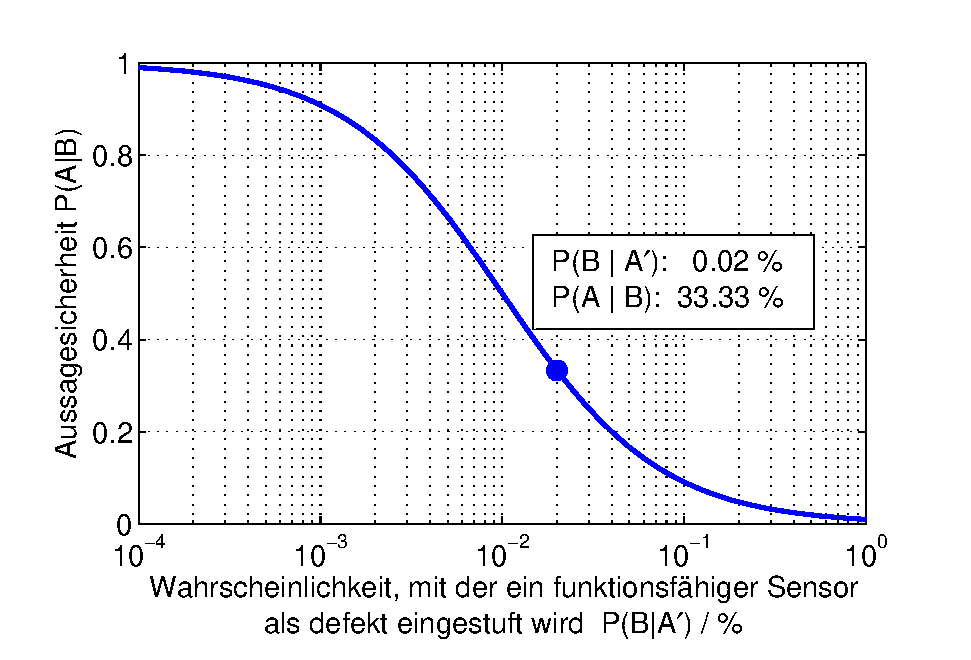
\includegraphics[width=0.5\textwidth]{Kapitel2/Bilder/image16}}
  \caption{Sprungantwort h(t) und Impulsantwort g(t) als Ausgangssignal eines energiefreien LTI-Systems}
  \label{fig:EnergiefreiLTI}
\end{figure}

\noindent F\"{u}r das Beispiel des RC-Netzwerks ergibt sich die Antwort auf einen Sprung der H\"{o}he U${}_{E0}$ = 1 mit der Bedingung u${}_{A}$(0) = 0 zu 

\begin{equation}\label{eq:threehundredfourtyeight}
h\left(t\right)={\rm \; }\left(1-e^{-\frac{t}{R\cdot C} } \right)\cdot \sigma \left(t\right)
\end{equation}

\noindent Wie bereits in Bild \ref{fig:EnergiefreiLTI} dargestellt ist die Impulsantwort g(t) eines Systems die Reaktion eines energiefreien Systems auf eine Anregung mit einem Impuls $\delta$(t). Im Kapitel Signale wird gezeigt, dass die Impulsfunktion $\delta$(t) als Ableitung der Sprungfunktion $\sigma$(t) gedeutet werden kann. 

\begin{equation}\label{eq:threehundredfourtynine}
\delta \left(t\right)=\frac{d\sigma }{dt}
\end{equation}

\noindent F\"{u}r lineare, zeitinvariante Systeme ergibt sich die Systemreaktion auf einen Impuls am Eingang aus der Ableitung der Sprungantwort.

\begin{equation}\label{eq:threehundredfifty}
g\left(t\right)=\frac{dh}{dt} 
\end{equation}

\noindent Bei bekannter Sprungantwort h(t) kann mit Gleichung \eqref{eq:threehundredfifty} die Impulsantwort g(t) durch Ableiten bestimmt werden. Zum Beispiel ergibt sich die Systemantwort eines RC-Netzwerks auf einen Impuls mit dem Gewicht U${}_{E0}$ = 1 mit der Produktregel zu

\begin{equation}\label{eq:threehundredfiftyone}
\begin{split}
g\left(t\right) & = \frac{dh}{dt} =\frac{d}{dt} {\rm \; }\left(\left(1-e^{-\frac{t}{R\cdot C} } \right)\cdot \sigma \left(t\right)\right)=\frac{1}{R\cdot C} \cdot e^{-\frac{t}{R\cdot C} } \cdot U_{E0} \cdot \sigma \left(t\right)-\left(1-e^{-\frac{t}{R\cdot C} } \right)\cdot \delta \left(t\right) \\ 
& = {\frac{1}{R\cdot C} \cdot e^{-\frac{t}{R\cdot C} } \cdot U_{E0} \cdot \sigma \left(t\right)}    
\end{split}
\end{equation}

\subsubsection{Berechnung der Systemantwort durch Superposition}\label{threethreefive}

\noindent Aufgrund der Linearität eines LTI-Systems kann die Systemantwort auf ein aus grundlegenden Funktionen zusammengesetztes Eingangssignal durch die entsprechende Kombination der Ausgangssignale bestimmt werden. Wird zum Beispiel das RC-Netzwerk aus Bild \ref{fig:RCSchaltbild} mit einer Rechteckfunktion der Länge t${}_{0}$ und der Höhe U${}_{E0}$ beaufschlagt, kann das Eingangssignal als Summe zweier Sprungfunktionen dargestellt werden

\begin{equation}\label{eq:threehundredfiftytwo}
u_{E} \left(t\right)=U_{E0} \cdot \left(\sigma \left(t\right)-\sigma \left(t-t_{0} \right)\right)=U_{E0} \cdot \sigma \left(t\right)-U_{E0} \cdot \sigma \left(t-t_{0} \right)
\end{equation}

\noindent Damit ergibt sich das Ausgangsignal u${}_{A}$ aus der Summe der beiden Sprungantworten

\begin{equation}\label{eq:threehundredfiftythree}
u_{A} \left(t\right)=U_{E0} \cdot \left(h\left(t\right)-h\left(t-t_{0} \right)\right)=U_{E0} \cdot \left(1-e^{-\frac{t}{R\cdot C} } \right)\cdot \sigma \left(t\right)-U_{E0} \cdot \left(1-e^{-\frac{t-t_{0} }{R\cdot C} } \right)\cdot \sigma \left(t-t_{0} \right)
\end{equation}

\noindent Bild \ref{fig:RCEinschwingenRechteck} stellt das Superpositionsprinzip für das Beispiel des RC-Netzwerks bei Anregung mit einem rechteckförmigen Signal dar.

\begin{figure}[H]
  \centerline{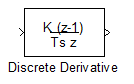
\includegraphics[width=1\textwidth]{Kapitel2/Bilder/image17}}
  \caption{Überlagerung der Systemreaktion u${}_{A}$ = u${}_{A1}$+ u${}_{A2}$ bei überlagertem Eingangssignal u${}_{E}$ = u${}_{E}$ + u${}_{E2}$}
  \label{fig:RCEinschwingenRechteck}
\end{figure}

\noindent Mit der Kenntnis der Sprungantwort eines Systems kann demnach für grundlegende Eingangs-signale, die sich über die Sprungfunktion darstellen lassen, eine Systemantwort berechnet werden. 

\subsection{Berechnung der Systemantwort über das Faltungsintegral}

\noindent In dem vorangegangenen Abschnitt werden mit der Linearitätseigenschaft und Zeitinvarianz eines Systems sowie der Sprungantwort h(t) Systemantworten auf andere Eingangssignale bestimmt. Die Näherung einer beliebigen Eingangsfunktion durch eine große Anzahl kleiner Impulse führt zur Bestimmung der Systemantwort über das Faltungsintegral, das im Folgenden hergeleitet wird. 

\subsubsection{Herleitung des Faltungsintegrals}

\noindent Ein lineares, zeitinvariantes System antwortet auf einen Impuls $\delta$(t) am Eingang mit der Impulsantwort g(t). Entsprechend antwortet es auf eine Linearkombination von Impulsen

\begin{equation}\label{eq:threehundredfiftyfour}
u\left(t\right)=\nu _{1} \cdot \delta \left(t\right)+\nu _{2} \cdot \delta \left(t-3\right)
\end{equation}

\noindent mit der gleichen Linearkombination von Impulsantworten

\begin{equation}\label{eq:threehundredfiftyfive}
y\left(t\right)=\nu _{1} \cdot g\left(t\right)+\nu _{2} \cdot g\left(t-3\right)
\end{equation}

\noindent Dieser Zusammenhang kann auf beliebige Eingangssignale verallgemeinert werden. Wegen der Ausblendeigenschaft der Impulsfunktion kann ein beliebiges Eingangssignal u(t) dargestellt werden als 

\begin{equation}\label{eq:threehundredfiftysix}
u\left(t\right)=u\left(t\right)\cdot \int\limits _{-\infty }^{\infty }\delta \left(t-\tau \right)\;d\tau  =\int\limits _{-\infty }^{\infty }u\left(t\right)\cdot \delta \left(t-\tau \right)\;d\tau  =\int\limits _{-\infty }^{\infty }u\left(\tau \right)\cdot \delta \left(t-\tau \right)\;d\tau 
\end{equation}

\noindent Anschaulich kann die Gleichung als Superposition unendlich vieler Impulse $\delta$(t - $\tau$) mit dem Gewicht u($\tau$) interpretiert werden, die zusammen das Signal u(t) darstellen. Jeder einzelne Impuls $\delta$(t - $\tau$) besitzt die Systemantwort g(t - $\tau$). Damit ergibt sich das Ausgangssignal y(t) aus der Superposition unendlich vieler Systemantworten g(t - $\tau$) mit dem Gewicht u($\tau$).

\begin{equation}\label{eq:threehundredfiftyseven}
y\left(t\right)=\int _{-\infty }^{\infty }u\left(\tau \right)\cdot g\left(t-\tau \right){\rm \; }d\tau  =u\left(t\right)*g\left(t\right)
\end{equation}

\noindent Bei bekannter Impulsantwort g(t) kann das Ausgangssignal y(t) für eine beliebige Systemanregung u(t) aus der Integralgleichung \eqref{eq:threehundredfiftyseven} berechnet werden. Das Integral wird als Faltungsintegral bezeichnet. Abkürzend wird die Faltungsoperation mit einem $*$ - Symbol dargestellt.

\subsubsection{Grafische Interpretation des Faltungsintegrals}

\noindent Das Faltungsintegral erscheint zunächst kompliziert und wenig griffig. Es kann aber grafisch interpretiert werden. Dazu wird das Faltungsintegral umgeformt zu

\begin{equation}\label{eq:threehundredfiftyeight}
y\left(t\right)=\int\limits _{-\infty }^{\infty }u\left(\tau \right)\cdot g\left(t-\tau \right)\;d\tau  =\int\limits _{-\infty }^{\infty }u\left(\tau \right)\cdot g\left(-\left(\tau -t\right)\right)\;d\tau 
\end{equation}

\noindent Das Faltungsintegral wird für einen festen Zeitpunkt t ausgewertet. Es ist die Fläche unter einer Funktion, die sich aus dem Produkt zweier Teilfunktionen ergibt. Eine Teilfunktion ist das bekannte Eingangssignal u($\tau$). Die zweite Teilfunktion ist die berechnete Impulsantwort g($\tau$), die jedoch an der Achse $\tau$ = 0 gespiegelt und um t nach rechts verschoben ist. \medskip

\noindent Aus dieser Interpretation ergibt sich folgendes Vorgehen zur grafischen Auswertung des Faltungsintegrals:

\begin{itemize}
\item  Skizzieren der Funktion u($\tau$)

\item  Skizzieren der Funktion g(-($\tau$ - t)) durch Spiegeln der Funktion g($\tau$) und Verschiebung um t nach rechts

\item  Berechnen des Produktes der beiden Funktionen u($\tau$)$.$g(-($\tau$ - t))

\item  Auswertung der Fl\"{a}che unter der Kurve u($\tau$)$.$g(-($\tau$ - t))
\end{itemize}

\noindent Das Verständnis der grafischen Faltung ist Grundlage für die Berechnung von Ausgangssignalen im Zeitbereich mit dem Faltungsintegral.\bigskip

\noindent
\colorbox{lightgray}{%
\arrayrulecolor{white}%
\renewcommand\arraystretch{0.6}%
\begin{tabular}{ wl{16.5cm} }
{\fontfamily{phv}\selectfont{
Beispiel: Grafische Faltung zweier Rechteckfunktionen}}
\end{tabular}%
}\bigskip

\noindent Das Vorgehen wird an der Faltung zweier Rechteckfunktionen verdeutlicht. 

\begin{equation}\label{eq:threehundredfiftynine}
u\left(t\right)=\sigma \left(t\right)-\sigma \left(t-2\right)
\end{equation}

\begin{equation}\label{eq:threehundredsixty}
g\left(t\right)=2\cdot \left(\sigma \left(t\right)-\sigma \left(t-4\right)\right)
\end{equation}

\noindent Zur grafischen Auswertung des Integrals werden beide Funktionen als Funktion der Variablen $\tau$ dargestellt, nach der integriert werden soll. 

\begin{equation}\label{eq:threehundredsixtyone}
u\left(\tau \right)=\sigma \left(\tau \right)-\sigma \left(\tau -2\right)
\end{equation}

\begin{equation}\label{eq:threehundredsixtytwo}
g\left(\tau \right)=2\cdot \left(\sigma \left(\tau \right)-\sigma \left(\tau -4\right)\right)
\end{equation}

\noindent Die Funktion g wird an der Achse $\tau$ = 0 gespiegelt 

\begin{equation}\label{eq:threehundredsixtythree}
g\left(-\tau \right)=2\cdot \left(\sigma \left(-\tau \right)-\sigma \left(-\left(\tau -4\right)\right)\right)
\end{equation}

\noindent und anschlie{\ss}end um t nach rechts verschoben. 

\begin{equation}\label{eq:threehundredsixtyfour}
g\left(t-\tau \right)=g\left(-\left(\tau -t\right)\right)=2\cdot \left(\sigma \left(-\left(\tau -t\right)\right)-\sigma \left(-\left(\tau -t-4\right)\right)\right)
\end{equation}

\noindent Bild \ref{fig:FaltungGrafischRechtecke} stellt die Funktionen f\"{u}r unterschiedliche Zeitpunkte t dar. Das Integral der Faltungsfunktion berechnet sich aus der Fl\"{a}che, die unter dem Produkt der beiden Funktionen u($\tau$) und g(t - $\tau$) liegt. F\"{u}r t = 0 \"{u}berschneiden sich die Funktionsbereiche, die ungleich null sind, nicht. Das Produkt der beiden Funktionen ist f\"{u}r t = 0 null. F\"{u}r negative Werte von t ist das ebenfalls der Fall, wie an dem Beispiel f\"{u}r t = - 1 deutlich wird. F\"{u}r positive Werte von t \"{u}berschneiden sich die Funktionsbereiche, in den die Funktionen ungleich null sind. Das gilt f\"{u}r den Bereich 0 $\leq$ t $\mathrm{<}$ 6. F\"{u}r den Bereich 2 $\leq$ t $\mathrm{<}$ 4 \"{u}berdecken sich die Funktionen komplett, hier ergibt sich ein konstanter Wert des Faltungsintegrals von 4, da die Fl\"{a}che in diesem Bereich konstant bleibt. F\"{u}r t $\mathrm{>}$ 6 liegt wieder keine \"{U}berschneidung vor, das Produkt der Funktionen ist f\"{u}r alle $\tau$ null.

\begin{figure}[H]
  \centerline{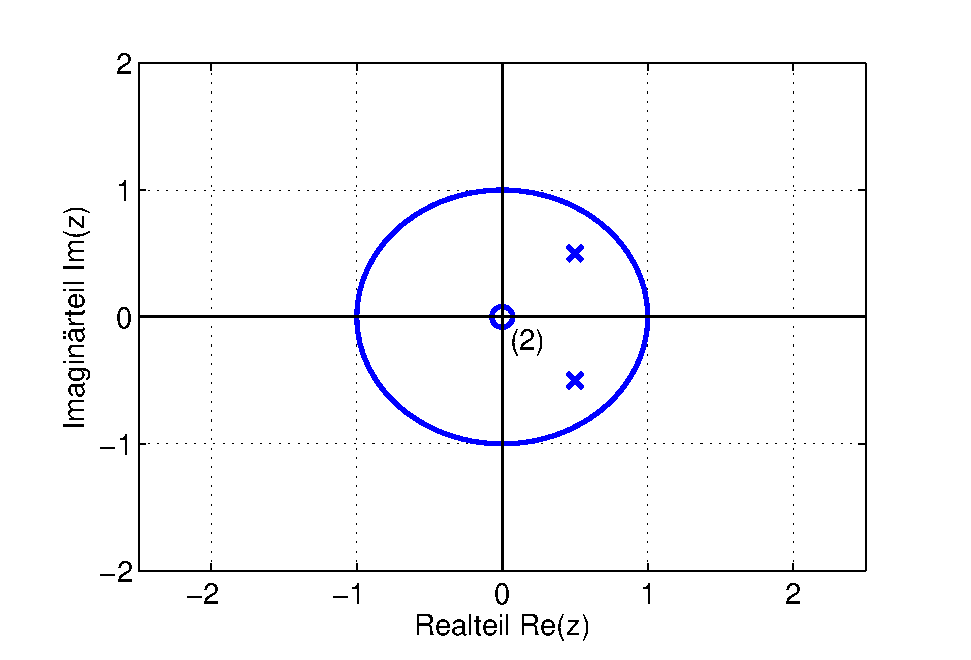
\includegraphics[width=1\textwidth]{Kapitel2/Bilder/image18}}
  \caption{Darstellung der Schritte zur grafischen Faltung am Beispiel zweier Rechtecke}
  \label{fig:FaltungGrafischRechtecke}
\end{figure}

\noindent Für einen festen Zeitpunkt t ergibt sich der Wert des Faltungsintegrals aus der Fläche unter der Rechteckfunktion. Durch Verschiebung der Funktion g ändert sich die Fläche, und es ergibt sich der in 
Bild \ref{fig:FaltungGrafischRechteckeBSP} dargestellte Verlauf des Faltungsintegrals.

\begin{figure}[H]
  \centerline{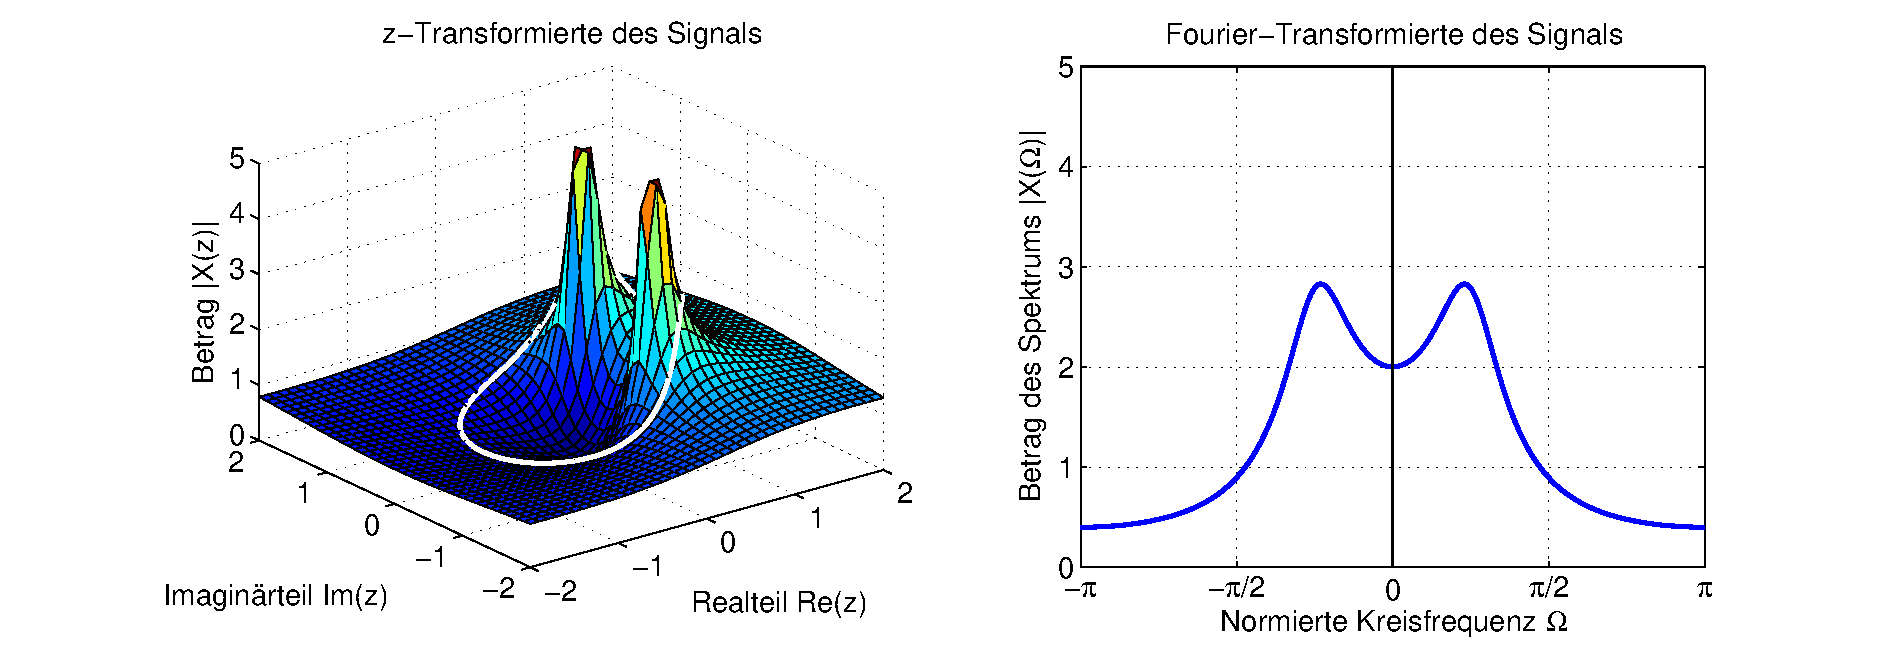
\includegraphics[width=0.5\textwidth]{Kapitel2/Bilder/image19}}
  \caption{Darstellung des Faltungsintegrals für das Beispiel zweier Rechtecke}
  \label{fig:FaltungGrafischRechteckeBSP}
\end{figure}

\noindent
\noindent

\InsertBoxL{0}{\includegraphics[scale=0.5]{code}} 
\textcolor{white}{.}\newline
\noindent Im Online-Portal \textit{Systemtheorie Online} verdeutlicht die Applikation \textit{Komplexe Exponentialfunktion} den Zusammenhang zwischen der Lage des Wertes $\lambda = \delta + j.\omega{}_{0}$ in der komplexen Ebene und dem Verhalten der Schwingung.\newline

\subsubsection{Rechenregeln zum Faltungsintegral}

\noindent Zur Berechnung des Faltungsintegrals existieren verschiedene Rechenregeln, die im Folgenden zusammengefasst werden. Die Herleitungen beruhen auf den Rechenregeln für Integrale und sind zum Beispiel in [Foel11] zu finden. Hier werden das Kommutativgesetz sowie die Rechen-regeln zur Faltung mit einem Impuls und die Faltung zweier kausaler Signale hergeleitet.\bigskip

\noindent\textbf{\fontfamily{phv}\selectfont{{Kommutativgesetz der Faltung}}}

\noindent In einigen Fällen ergeben sich Rechenvorteile, wenn das Kommutativgesetz der Faltung genutzt werden kann. Die Herleitung beginnt mit der Definitionsgleichung des Faltungsintegrals.

\begin{equation}\label{eq:threehundredsixtyfive}
y\left(t\right)=\int\limits _{-\infty }^{\infty }u\left(\tau \right)\cdot g\left(t-\tau \right)\;d\tau
\end{equation}

\noindent Mit der Substitution

\begin{equation}\label{eq:threehundredsixtysix}
\tau =t-x
\end{equation}

\noindent und der Ableitung

\begin{equation}\label{eq:threehundredsixtyseven}
\frac{d\tau }{dx} =-1
\end{equation}

\noindent ergibt sich 

\begin{equation}\label{eq:threehundredsixtyeight}
\begin{split}
y\left(t\right) & = \int\limits _{-\infty }^{\infty }u\left(\tau \right)\cdot g\left(t-\tau \right)\;d\tau  =-\int\limits _{\infty }^{-\infty }u\left(t-x\right)\cdot g\left(x\right)\;dx =\int\limits _{-\infty }^{\infty }u\left(t-x\right)\cdot g\left(x\right)\;dx \\
& = \int\limits _{-\infty }^{\infty } u\left(t-\tau\right)\cdot g(\tau) \; d\tau
\end{split}
\end{equation}

\noindent Das Ergebnis ist wieder ein Faltungsintegral. Allerdings wird bei diesem Faltungsintegral die Funktion u(t) an der Achse $\tau$ = 0 gespiegelt und um t verschoben. Es gilt das Kommutativgesetz.

\begin{equation}\label{eq:threehundredsixtynine}
u\left(t\right)*g\left(t\right)=g\left(t\right)*u\left(t\right)
\end{equation}

\noindent Der Integrand ist an allen Stellen null, nur nicht an der Stelle $\tau$ = t$_{0}$. Damit kann das Integral umgeformt werden zu

\begin{equation}\label{eq:threehundredseventy}
u\left(t\right)*\delta \left(t-t_{0} \right)=\int\limits _{-\infty }^{\infty }u\left(t-\tau \right)\cdot \delta \left(\tau -t_{0} \right)\;d\tau
\end{equation}

\noindent Der Integrand ist an allen Stellen null, nur nicht an der Stelle $\tau$ = t${}_{0}$. Damit kann das Integral umgeformt werden zu

\begin{equation}\label{eq:threehundredseventyone}
\int\limits _{-\infty }^{\infty }u\left(t-\tau \right)\cdot \delta \left(\tau -t_{0} \right){\rm \; }d\tau  =u\left(t-t_{0} \right)\cdot \int\limits _{-\infty }^{\infty }\delta \left(\tau -t_{0} \right){\rm \; }d\tau 
\end{equation}

\noindent Da das Integral \"{u}ber eine Impulsfunktion immer eins ist, ergibt sich

\begin{equation}\label{eq:threehundredseventytwo}
u\left(t\right)*\delta \left(t-t_{0} \right)=u\left(t-t_{0} \right)\cdot \int\limits _{-\infty }^{\infty }\delta \left(\tau -t_{0} \right)\;d\tau  =u\left(t-t_{0} \right)
\end{equation}

\noindent Die Faltung eines Signals u(t) mit einem Impuls an der Stelle t${}_{0}$ verschiebt das Signal an die Stelle des Impulses. \bigskip

\noindent
\colorbox{lightgray}{%
\arrayrulecolor{white}%
\renewcommand\arraystretch{0.6}%
\begin{tabular}{ wl{16.5cm} }
{\fontfamily{phv}\selectfont
\noindent
Beispiel: Grafische Faltung eines Signals mit einem Impuls}
\end{tabular}%
}\bigskip

\noindent Bild \ref{fig:FaltungGrafischImpuls} stellt die Faltung eines Signals mit einem um t${}_{0}$ = 6 verschobenen Impuls dar. Das Ergebnis kann so hergeleitet werden, dass der Impuls $\deltaup$(t - 6 - $\tau$) an dem Signal u(t) vorbei geschoben wird. Das Produkt der beiden Signale ist nur in dem Bereich 4 $\leq$ t $\mathrm{<}$ 8 ungleich null, in den anderen Bereichen ist mindestens eine der beiden Funktionen null.

\begin{figure}[H]
  \centerline{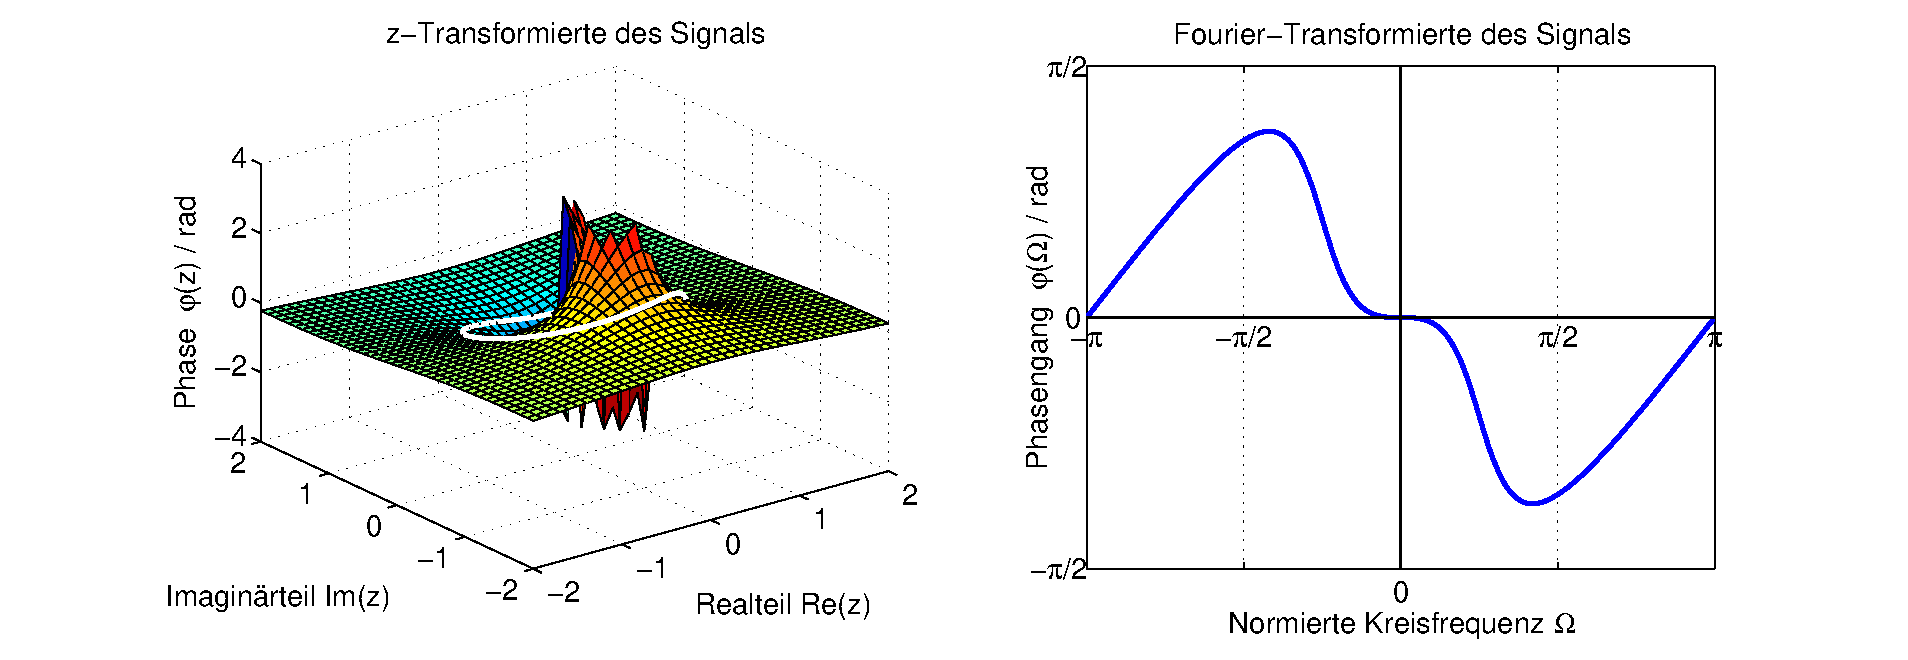
\includegraphics[width=1\textwidth]{Kapitel2/Bilder/image20}}
  \caption{Grafische Faltung eines Signals u(t) mit einem Impuls an der Stelle t$_{0}$ = 6}
  \label{fig:FaltungGrafischImpuls}
\end{figure}

\noindent Die Auswertung der grafischen Faltung ist in Bild \ref{fig:FaltungGrafischImpulsBSP} dargestellt. Die Funktion u(t) ist um t$_{0}$ nach rechts verschoben worden.

\begin{figure}[H]
  \centerline{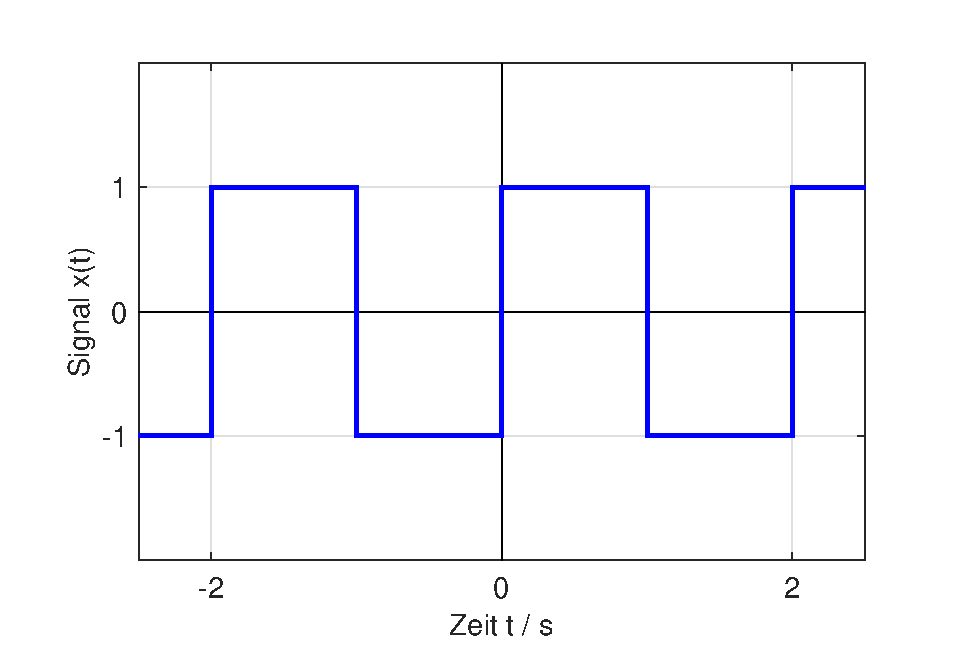
\includegraphics[width=0.5\textwidth]{Kapitel2/Bilder/image21}}
  \caption{Ergebnis der grafischen Faltung eines Signals u(t) mit einem Impuls an der Stelle t$_{0}$ = 6}
  \label{fig:FaltungGrafischImpulsBSP}
\end{figure}

\clearpage

{\fontfamily{phv}\selectfont
\noindent\textbf{Faltung kausaler Funktionen}}\smallskip

\noindent Sind die Funktionen g(t) und u(t) kausale Funktionen, reduziert sich das Faltungsintegral auf den Bereich von 0 … t. Dieses Ergebnis ergibt sich unmittelbar aus der grafischen Faltung. 

\begin{figure}[H]
  \centerline{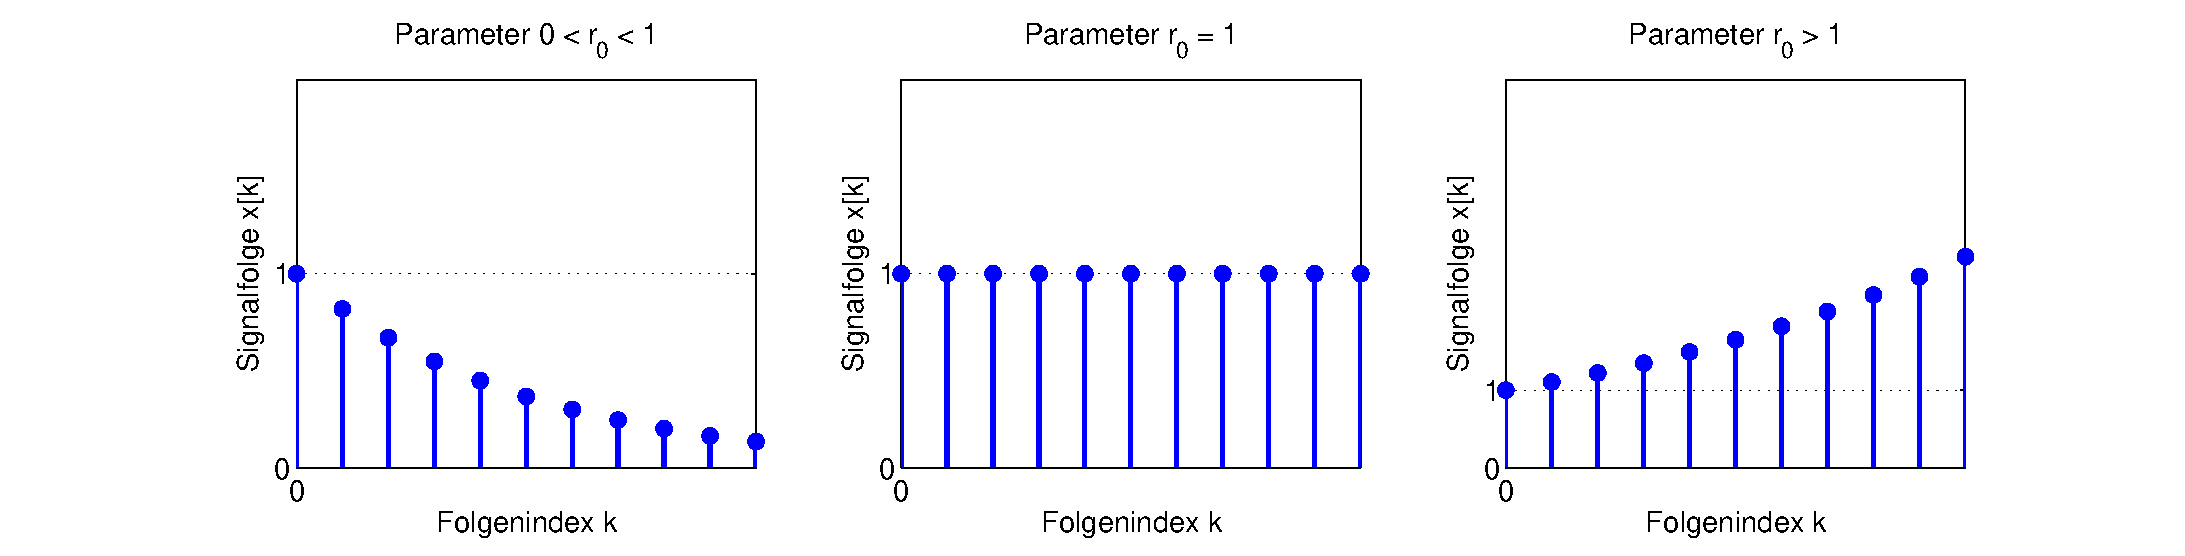
\includegraphics[width=1\textwidth]{Kapitel2/Bilder/image22}}
  \caption{Faltung kausaler Funktionen}
  \label{fig:FaltungKausal}
\end{figure}

\noindent Die Funktion u($\tau$) ist f\"{u}r den Bereich $\tau$ $\mathrm{<}$ 0 null, die Funktion g(t - $\tau$) ist f\"{u}r den Bereich $\tau$ $\mathrm{>}$ t null. Damit ist das Produkt der beiden Funktionen nur in dem Bereich von 0 {\dots} t von null verschieden. F\"{u}r kausale Funktionen gilt deshalb

\begin{equation}\label{eq:threehundredseventythree}
y\left(t\right)=\int _{-\infty }^{\infty }u\left(\tau \right)\cdot g\left(t-\tau \right){\rm \; }d\tau  =\int _{0}^{t}u\left(\tau \right)\cdot g\left(t-\tau \right){\rm \; }d\tau 
\end{equation}

\clearpage

{\fontfamily{phv}\selectfont
\noindent\textbf{Zusammenfassung der Rechenregeln zum Faltungsintegral}}

\noindent Die wesentlichen Rechenregeln für das Faltungsintegral sind in Tabelle 3.8 zusammengefasst.

\begin{table}[H]
\caption{Zusammenhang zwischen Lösungen der charakteristischen Gleichung und der Stabilität von LTI-Systemen, die sich über lineare Differentialgleichungen mit konstanten Koeffizienten beschreiben lassen }
\setlength{\fboxsep}{0pt}%
\colorbox{lightgray}{%
\arrayrulecolor{white}%
\begin{tabular}{| c | c |}
\hline
\parbox[c][0.28in][c]{3.3in}{\smallskip\centering\textbf{\fontfamily{phv}\selectfont{Gesetz}}} & \parbox[c][0.28in][c]{3.3in}{\smallskip\centering\textbf{\fontfamily{phv}\selectfont{Mathematische Beschreibung}}}\\ \hline

\parbox[c][0.7in][c]{3.3in}{\centering{\fontfamily{phv}\selectfont{Kommutativgesetz}}} &
\parbox[c][0.7in][c]{3.3in}{\centering{
$u\left(t\right)*g\left(t\right)=g\left(t\right)*u\left(t\right)$
}}\\ \hline

\parbox[c][0.8in][c]{3.3in}{\centering{\fontfamily{phv}\selectfont{Assoziativgesetz}}} & 
\parbox[c][0.8in][c]{3.3in}{\centering{
$\left(x\left(t\right)*u\left(t\right)\right)*g\left(t\right)=x\left(t\right)*\left(u\left(t\right)*g\left(t\right)\right)$
}}\\ \hline

\parbox[c][0.8in][c]{3.3in}{\centering{\fontfamily{phv}\selectfont{Distributivgesetz}}} &
\parbox[c][0.8in][c]{3.3in}{\centering{
$\left(u_{1} \left(t\right)+u_{2} \left(t\right)\right)*g\left(t\right)=u_{1} \left(t\right)*g\left(t\right)+u_{2} \left(t\right)*g\left(t\right)$
}}\\ \hline

\parbox[c][0.8in][c]{3.3in}{\centering{\fontfamily{phv}\selectfont{Faltung kausaler Signale}}} &
\parbox[c][0.8in][c]{3.3in}{\centering{
$\int _{-\infty }^{\infty }u\left(\tau \right)\cdot g\left(t-\tau \right){\rm \; }d\tau  =\int _{0}^{t}u\left(\tau \right)\cdot g\left(t-\tau \right){\rm \; }d\tau  $ 
}}\\ \hline

\parbox[c][0.8in][c]{3.3in}{\centering{\fontfamily{phv}\selectfont{Faltung mit einem Impuls an der Stelle $t_{0}$}}} &
\parbox[c][0.8in][c]{3.3in}{\centering{
$u\left(t\right)*\delta \left(t-t_{0} \right)=u\left(t-t_{0} \right)$
}}\\ \hline

\end{tabular}%
}\bigskip
\label{tab:threeeight}
\end{table}

\subsubsection{Anwendung des Faltungsintegrals am Beispiel des RC-Netzwerks}\label{threefourfour}

\noindent Die Berechnung des Faltungsintegrals wird an einem RC-Netzwerk vertieft, das mit einem recht-eckförmigen Signal angeregt wird. Das Ergebnis wird anschließend mit dem Ergebnis verglichen, das sich bei Anwendung des Superpositionsprinzips ergeben hat. Die Impulsantwort g(t) des RC-Netzwerks lautet

\begin{equation}\label{eq:threehundredseventyfour}
g\left(t\right)=\frac{1}{R\cdot C} \cdot e^{-\frac{t}{R\cdot C} } \cdot \sigma \left(t\right)
\end{equation}

\noindent Das Eingangssignal ist definiert als

\begin{equation}\label{eq:threehundredseventyfive}
u_{E} \left(t\right)=\left\{\begin{array}{l} 
{U_{{\rm E0}} \qquad  \text{ für } \; 0\le  t<\rm t_{0} } \\ 
0\qquad \quad \;\, \text{sonst}
\end{array}\right.
\end{equation}

\noindent Beide Signale sind kausal, sodass sich das Ausgangssignal u${}_{A}$(t) ergibt

\begin{equation}\label{eq:threehundredseventysix}
u_{A} \left(t\right)=\int _{0}^{t}u_{E} \left(\tau \right)\cdot g\left(t-\tau \right)\;d\tau
\end{equation}

\noindent Zur Auswertung des Integrals muss analysiert werden, wann sich die beiden Funktionen g(t - $\tau$) und u${}_{E}$($\tau$) \"{u}berlappen. Dazu zeigt Bild \ref{fig:FaltungGrafischRCNetzwerk} die Funktionen g(t - $\tau$) und u${}_{E}$($\tau$) f\"{u}r unterschiedliche Zeitpunkte t.

\begin{figure}[H]
  \centerline{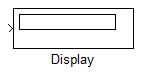
\includegraphics[width=1\textwidth]{Kapitel2/Bilder/image23}}
  \caption{Darstellung der Funktionen g(t - $\tau$) und u${}_{E}$($\tau$) zur Berechnung des Faltungsintegrals f\"{u}r verschiedene Zeitpunkte t}
  \label{fig:FaltungGrafischRCNetzwerk}
\end{figure}\bigskip

{\fontfamily{phv}\selectfont
\noindent\textbf{Zeitraum  t $\mathrm{<}$ 0}}\smallskip

\noindent F\"{u}r alle $\tau$ ist zumindest eine der beiden Funktionen null, das Faltungsintegral ist damit f\"{u}r t $\mathrm{<}$ 0 null.

\begin{equation}\label{eq:threehundredseventyseven}
u_{A} \left(t\right)=0
\end{equation}\bigskip

{\fontfamily{phv}\selectfont
\noindent\textbf{Zeitraum 0 $\mathrm{<}$ t $\mathrm{<}$ t$_{0}$}}\smallskip

\noindent Die beiden Funktionen \"{u}berlappen sich in dem Bereich 0 $\leq$ $\tau$ $\leq$ t, sodass das Integral in diesem Bereich ausgef\"{u}hrt wird. 

\begin{equation}\label{eq:threehundredseventyeight}
\begin{split}
u_{A} \left(t\right) & = \int\limits _{0}^{t}g\left(t-\tau \right)\cdot U_{E0} \;d\tau  =\int\limits _{0}^{t}U_{E0} \cdot \frac{1}{R\cdot C} \cdot e^{-\frac{t-\tau }{RC} } \;d\tau  =e^{-\frac{t}{RC} } \cdot \int\limits _{0}^{t}U_{E0} \cdot \frac{1}{R\cdot C} \cdot e^{\frac{\tau }{RC} } \;d\tau\\
& =\left. U_{E0}\cdot\frac{1}{R\cdot C}\cdot e^{-\frac{t}{R\cdot C}}\cdot R\cdot C \cdot  e^{\frac{t}{R\cdot C}}\right|_{0}^{t} 
=  U_{E0}\cdot \frac{1}{R\cdot C}\cdot e^{-\frac{t}{R\cdot C}}\cdot R\cdot C (\cdot  e^{\frac{t}{R\cdot C}}-e^{\frac{0}{R\cdot C}})\\
& =  U_{E0} \cdot (1-e^{-\frac{t}{R\cdot C}})
\end{split}
\end{equation}\bigskip
\clearpage

{\fontfamily{phv}\selectfont
\noindent\textbf{Zeitraum t $\geqslant $ t$_{0}$}}\smallskip

\noindent Jetzt überlappen sich die beiden Funktionen ganz und die Integration erstreckt sich von 0 bis t$_{0}$.

\begin{equation}\label{eq:threehundredseventynine}
\begin{split}
u_{A} \left(t\right) & = \int\limits _{0}^{t_{0} }g\left(t-\tau \right)\cdot U_{E0} \;d\tau  =\int\limits _{0}^{t_{0} }U_{E0} \cdot \frac{1}{R\cdot C} \cdot e^{-\frac{t-\tau }{RC} } \; d\tau  =\left. U_{E0} \cdot \frac{1}{R\cdot C} \cdot e^{-\frac{t}{R\cdot C} } \cdot R\cdot C\cdot e^{\frac{\tau }{R\cdot C} } \right|_{0}^{t_{0}} \\ 
& = U_{E0} \cdot e^{-\frac{t}{R\cdot C}} \cdot (e^{\frac{t_{0}}{R\cdot C}}-1) = U_{E0} \cdot (1-e^{-\frac{t_{0}}{R\cdot C}}) \cdot e^{-\frac{t-t_{0}}{R\cdot C}}
\end{split}
\end{equation}

\noindent Damit kann u$_{A}$(t) zusammengefasst werden als

\begin{equation}\label{eq:threehundredeighty}
\begin{split}
u_{A} \left(t\right)=\left\{\begin{array}{l} 
{U_{E0} \cdot \left(1-e^{-\frac{t}{RC} } \right) \qquad \qquad \quad \text{für } 0\leqslant t<t_{0} }\medskip \\ 
{U_{E0} \cdot \left(1-e^{-\frac{t_{0} }{R\cdot C}} \right)\cdot e^{-\frac{t-t_{0} }{R\cdot C}} \qquad \; \text{für } t \ge t_{0\qquad } } \\ 
{} \\ 0 \; \qquad \qquad \qquad \qquad \qquad \quad \text{sonst} 
\end{array}\right.
\end{split}
\end{equation}

\noindent Das Ergebnis stimmt erwartungsgemäß mit dem Ergebnis in Gleichung (\ref{eq:threehundredfiftythree}) überein\bigskip

{\fontfamily{phv}\selectfont
\noindent\textbf{Zusammenfassung Faltungsintegral}}\smallskip

\noindent Die in diesem Beispiel dargestellte Methode zur Berechnung des Faltungsintegrals besteht aus folgenden Schritten:

\begin{table}[H]
\caption{Vorgehen bei der Berechnung der Systemantwort über das Faltungsintegral}
\setlength{\fboxsep}{0pt}%
\colorbox{lightgray}{%
\arrayrulecolor{white}%
\begin{tabular}{| c | c |}
\hline
\parbox[c][0.28in][c]{0.45in}{\smallskip\centering\textbf{\fontfamily{phv}\selectfont{Schritt}}} & \parbox[c][0.28in][c]{6in}{\smallskip\centering\textbf{\fontfamily{phv}\selectfont{Beschreibung}}}\\ \hline

\parbox[c][0.4in][c]{0.45in}{\centering{1}} &
\parbox[c][0.4in][c]{6in}{\centering{\fontfamily{phv}\selectfont{
Berechnung der Impulsantwort
}}}\\ \hline

\parbox[c][0.4in][c]{0.45in}{\centering{2}} & \parbox[c][0.4in][c]{6in}{\centering{\fontfamily{phv}\selectfont{
Skizze von Eingangssignal u($\tau$) und Impulsantwort $g(\tau)$
}}}\\ \hline

\parbox[c][0.6in][c]{0.45in}{\centering{3}} &
\parbox[c][0.6in][c]{6in}{\centering{\fontfamily{phv}\selectfont{
Skizze von einem der Signale $u(t - \tau)$ oder $g(t - \tau)$ über Spiegelung an der Achse $\tau$ = 0 und 
Verschiebung um t nach rechts
}}}\\ \hline

\parbox[c][0.4in][c]{0.45in}{\centering{4}} &
\parbox[c][0.4in][c]{6in}{\centering{\fontfamily{phv}\selectfont{
Aufteilen des Faltungsintegrals in sinnvolle Zeitbereiche \\
(Überlappungsbereiche, Sprungstellen, Definitionsgrenzen, ...)
}}}\\ \hline

\parbox[c][0.4in][c]{0.45in}{\centering{5}} &
\parbox[c][0.4in][c]{6in}{\centering{\fontfamily{phv}\selectfont{
Lösen der Integrale und Superposition der Ergebnisse
}}}\\ \hline

\end{tabular}%
}\bigskip
\label{tab:threenine}
\end{table}

\noindent Die Berechnung des Faltungsintegrals ist aufwendig. Es wird sich zeigen, dass die Berechnung eines Ausgangsignals im Laplace-Bereich deutlich einfacher ist als im Zeitbereich.

\subsubsection{Impulsantwort und Stabilität}\label{threefourfive}

\noindent In Abschnitt \ref{threetwothree} wird die Stabilit\"{a}t von Systemen aus physikalischer Sicht definiert. Mit dem Wissen, dass sich bei einem LTI-System die Systemantwort y(t) aus dem Faltungsintegral ergibt, kann die Stabilit\"{a}tsbewertung auf die Impulsantwort g(t) zur\"{u}ckgef\"{u}hrt werden. Dabei wird davon ausgegangen, dass das System in einem Zeitraum 0 $\mathrm{<}$ t $\leq$ t${}_{0}$ angeregt wird. Zur Stabilit\"{a}tsbewertung wird das Ausgangssignal nach der Anregung t $\geq$ t${}_{0}$ analysiert. In diesem Zeitraum gilt:

\begin{equation}\label{eq:threehundredeightyone}
y\left(t\right)=\int _{0}^{t_{0} }u\left(\tau \right)\cdot g\left(t-\tau \right)\;d\tau
\end{equation}

\noindent Aus der physikalischen Bedingung an asymptotische Stabilit\"{a}t leitet sich die Forderung ab, dass bei einer zeitlich begrenzten Anregung das Ausgangssignal den Grenzwert 

\begin{equation}\label{eq:threehundredeightytwo}
{\mathop{\lim }\limits_{t\to \infty }} \; \left|y\left(t\right)\right|=0
\end{equation}

\noindent aufweisen muss. Ist der Betrag des Eingangssignals beschr\"{a}nkt, kann er mit {\textbar}u($\tau$){\textbar} $\mathrm{<}$ u${}_{MAX}$ abgesch\"{a}tzt werden, und der Betrag des Ausgangssignals ergibt sich zu

\begin{equation}\label{eq:threehundredeightythree}
\left|y\left(t\right)\right|\le \int\limits _{0}^{t_{0} }\left|u\left(\tau \right)\right|\cdot \left|g\left(t-\tau \right)\right|\;d\tau  <u_{MAX} \cdot \int\limits _{0}^{t_{0} }\left|g\left(t-\tau \right)\right|\;d\tau 
\end{equation}

\noindent Es handelt sich um ein endliches Integral, das zu null wird, wenn die Impulsantwort g(t) gegen null konvergiert.

\begin{equation}\label{eq:threehundredeightyfour}
{\mathop{\lim }\limits_{t\to \infty }} \; g\left(t\right)=0
\end{equation}

\noindent Ein System ist damit asymptotisch stabil, wenn die Impulsantwort gegen null konvergiert. Aus der physikalischen Bedingung an grenzstabile Systeme leitet sich die Forderung ab, dass bei einer zeitlich begrenzten Anregung das Ausgangssignal den Grenzwert 

\begin{equation}\label{eq:threehundredeightyfive}
{\mathop{\lim }\limits_{t\to \infty }} \; \left|y\left(t\right)\right|=y_{0} <\infty 
\end{equation}

\noindent aufweisen muss. Das Ausgangssignal y(t) errechnet sich f\"{u}r Impulsantworten g(t), die f\"{u}r t $\rightarrow$ $\mathrm{\infty}$ einem konstanten Wert g${}_{0}$ zustreben, \"{u}ber 

\begin{equation}\label{eq:threehundredeightysix}
{\mathop{\lim }\limits_{t\to \infty }} \, \, y\left(t\right)=\int _{0}^{t_{0} }u\left(\tau \right)\cdot g\left(t-\tau \right)\;d\tau  =g_{0} \cdot \int _{0}^{t_{0} }u\left(\tau \right)\;d\tau  =y_{0} \ne 0
\end{equation}

\noindent Das Ausgangssignal konvergiert f\"{u}r t $\geq$ t${}_{0}$ gegen einen konstanten Wert. Systeme, deren Impulsantworten g(t) f\"{u}r t $\rightarrow$ $\mathrm{\infty}$ einem konstanten Wert g${}_{0}$ zustreben, entsprechen damit den Bedingungen grenzstabiler Systeme. Dasselbe gilt f\"{u}r Systeme, deren Impulsantwort f\"{u}r t $\rightarrow$ $\mathrm{\infty}$ mit konstanter Amplitude schwingt. Der Nachweis wird in eine \"{U}bungsaufgabe erbracht. Aus Gleichung \eqref{eq:threehundredeightythree} wird deutlich, dass das Ausgangssignal y(t) bei divergierender Impulsantwort ebenfalls divergiert. Systeme mit divergierender Impulsantwort sind damit instabil. Der Zusammenhang zwischen Impulsantwort und Stabilit\"{a}t linearer, zeitinvarianter Systeme ist in Tabelle \ref{tab:threeten} zusammengefasst.

\begin{table}[H]
\caption{Zusammenhang zwischen Lösungen der charakteristischen Gleichung und der Stabilität von LTI-Systemen, die sich über lineare Differentialgleichungen mit konstanten Koeffizienten beschreiben lassen }
\setlength{\fboxsep}{0pt}%
\colorbox{lightgray}{%
\arrayrulecolor{white}%
\begin{tabular}{| c | c |}
\hline
\parbox[c][0.28in][c]{3.3in}{\smallskip\centering\textbf{\fontfamily{phv}\selectfont{Eigenschaft}}} & \parbox[c][0.28in][c]{3.3in}{\smallskip\centering\textbf{\fontfamily{phv}\selectfont{Bedeutung}}}\\ \hline

\parbox[c][0.4in][c]{3.3in}{\centering{\fontfamily{phv}\selectfont{Asymptotisch stabiles System}}} &
\parbox[c][0.4in][c]{3.3in}{\centering{
$\lim_{t\to \infty}  g(t)=0$
}}\\ \hline

\parbox[c][0.9in][c]{3.3in}{\centering{\fontfamily{phv}\selectfont{Grenzstabiles System}}} & 
\parbox[c][0.9in][c]{3.3in}{\centering{\fontfamily{phv}\selectfont{
$\lim_{t\to \infty}$  g(t)=g$_{0}$ $\ne$ 0 \\
oder \\
harmonische Schwingung mit konstanter Amplitude
}}}\\ \hline

\parbox[c][0.4in][c]{3.3in}{\centering{\fontfamily{phv}\selectfont{Instabiles System}}} &
\parbox[c][0.4in][c]{3.3in}{\centering{\fontfamily{phv}\selectfont{
$\lim_{t\to \infty}$ g(t) ist divergent
}}}\\ \hline

\end{tabular}%
}\bigskip
\label{tab:threeten}
\end{table}

\noindent Zur Stabilitätsbewertung von Systemen im Zeitbereich muss die Impulsantwort bekannt sein. Es wird sich zeigen, dass eine Bewertung der Stabilität im Laplace-Bereich praktikabler vorgenom-men werden kann.\bigskip

\noindent
\colorbox{lightgray}{%
\arrayrulecolor{white}%
\renewcommand\arraystretch{0.6}%
\begin{tabular}{ wl{16.5cm} }
{\fontfamily{phv}\selectfont{
Beispiel: RC-Netzwerk als stabiles System}}
\end{tabular}%
 b}\bigskip

\noindent Das diskutierte RC-Netzwerk weist eine Impulsantwort

\begin{equation}\label{eq:threehundredeightyseven}
g\left(t\right)=\frac{1}{R\cdot C} \cdot e^{-\frac{t}{R\cdot C} \cdot t} \cdot \sigma \left(t\right)
\end{equation}

\noindent auf. Die Impulsantwort wird auf absolute Integrierbarkeit gepr\"{u}ft.

\begin{equation}\label{eq:threehundredeightyeight}
\int\limits _{-\infty }^{\infty }\left|g\left(t\right)\right|\;dt =\int\limits _{-\infty }^{\infty }\frac{1}{R\cdot C} \cdot e^{-\frac{t}{R\cdot C} } \cdot \sigma \left(t\right)\;dt =\frac{1}{R\cdot C} \cdot \int\limits _{0}^{\infty }e^{-\frac{t}{R\cdot C} } \;dt =-\frac{R\cdot C}{R\cdot C} \cdot \left. e^{-\frac{t}{R\cdot C} } \right|_{0}^{\infty } =-\left(0-1\right)=1<\infty
\end{equation}

\noindent Die Impulsantwort ist absolut integrierbar, das System ist demnach stabil. Das zeigt sich auch an dem Ausgangssignal des RC-Glieds auf eine Anregung mit einem Rechtecksignal.

\begin{figure}[H]
  \centerline{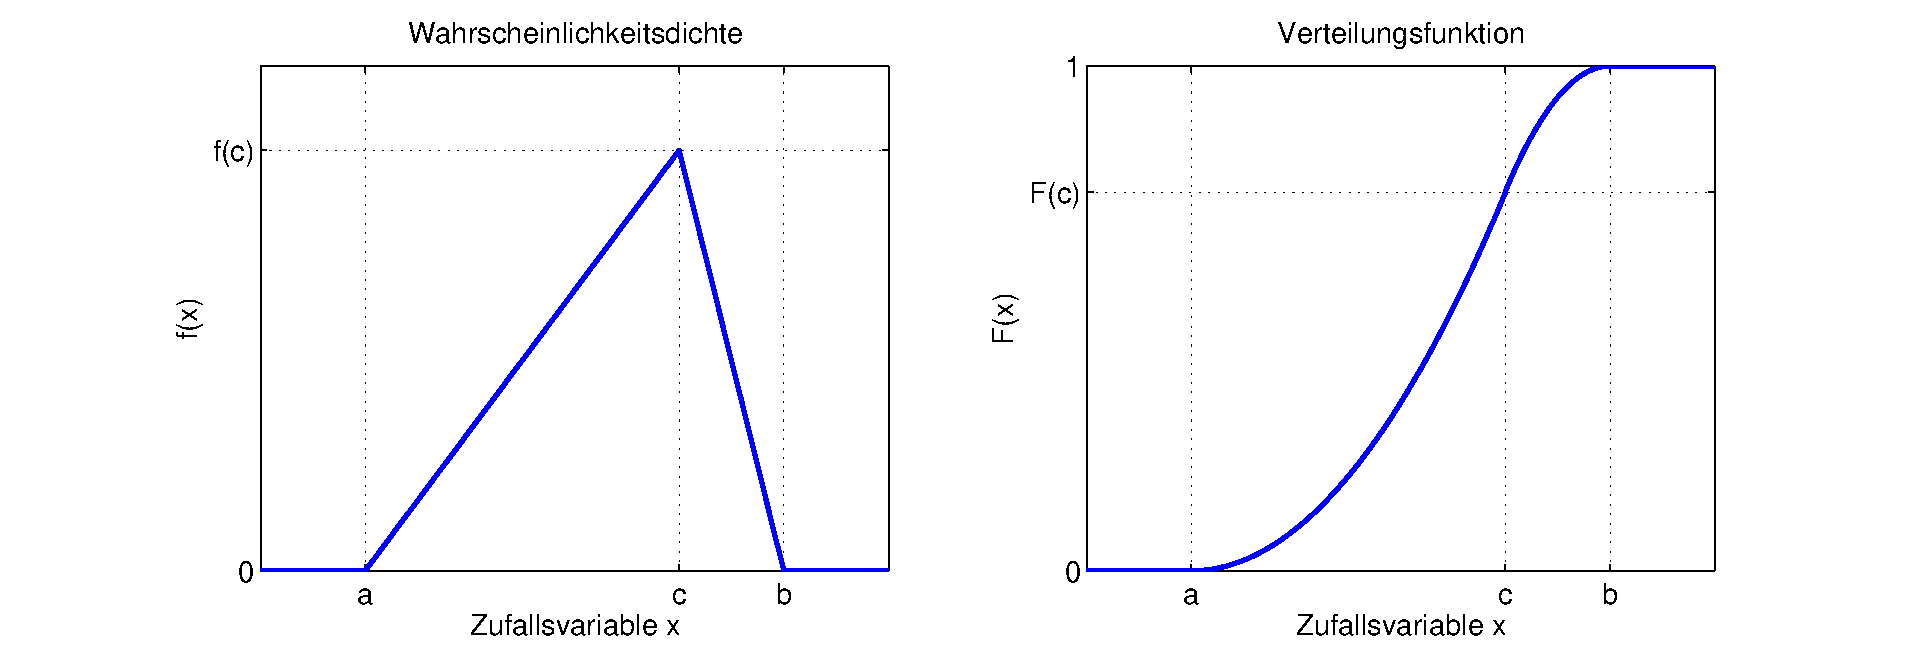
\includegraphics[width=0.5\textwidth]{Kapitel2/Bilder/image24.eps}}
  \caption{Anregung eines RC-Glieds mit einem Rechtecksignal}
  \label{fig:inconnue}
\end{figure}

\noindent Nach der Anregung klingt das Ausgangssignal ab und erreicht f\"{u}r t $\rightarrow$ $\mathrm{\infty}$ den Wert null.\bigskip

\noindent
\colorbox{lightgray}{%
\arrayrulecolor{white}%
\renewcommand\arraystretch{0.6}%
\begin{tabular}{ wl{16.5cm} }
{\fontfamily{phv}\selectfont
\noindent
Beispiel: Integrierer als grenzstabiles System}
\end{tabular}%
}\bigskip

\noindent Als Beispiel für ein grenzstabiles System wird ein Integrierer hinsichtlich seiner Stabilität bewertet. Er besitzt die Impulsantwort

\begin{equation}\label{eq:threehundredeightynine}
g\left(t\right)=\int\limits _{-\infty }^{t}\delta \left(\tau \right) \;\tau =\sigma \left(t\right)
\end{equation}

\noindent Die Impulsantwort besitzt f\"{u}r t $\rightarrow$ $\mathrm{\infty}$ den konstanten Wert g${}_{0}$ = 1, das System ist demnach grenzstabil. Wird als Eingangssignal ein Rechtecksignal 

\begin{equation}\label{eq:threehundredninety}
u\left(t\right)=\sigma \left(t\right)-\sigma \left(t-2\right)
\end{equation}

\noindent gewählt, ergibt sich das Ausgangssignal durch grafische Faltung zu

\begin{equation}\label{eq:threehundredninetyone}
y\left(t\right)=t\cdot \sigma \left(t\right)-\left(t-2\right)\cdot \sigma \left(t-2\right)
\end{equation}

\noindent Bild \ref{fig:FaltungIntegrierer} zeigt die Antwort y(t) des Integrierers auf das Rechteck-Signal am Eingang.

\begin{figure}[H]
  \centerline{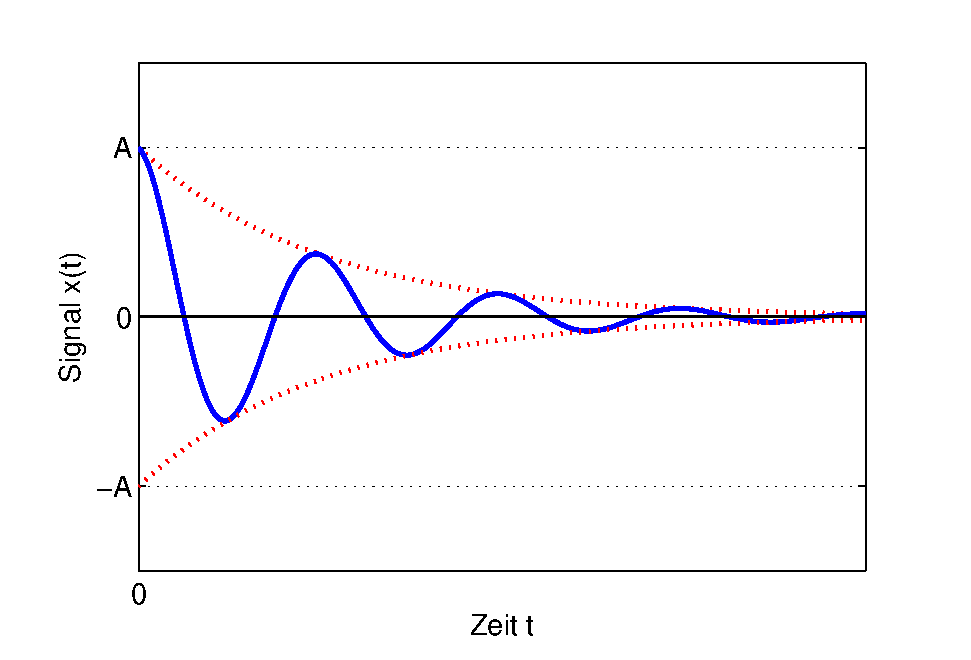
\includegraphics[width=1\textwidth]{Kapitel2/Bilder/image25}}
  \caption{Verhalten eines Integrierers als Beispiel für ein grenzstabiles System}
  \label{fig:FaltungIntegrierer}
\end{figure}

\noindent Wird das Eingangssignal zeitlich begrenzt, besitzt der Integrierer ein endliches Ausgangssignal. Damit ist bestätigt, dass der Integrierer ein grenzstabiles System ist. 


\subsection{Simulation linearer, zeitinvarianter Systeme}

\noindent Die Beschreibung dynamischer Systeme kann über mathematische Funktionen erfolgen. Die analytische Berechnung von Systemreaktionen ist wichtig, um Systeme zu interpretieren und zu charakterisieren.
Ihre Berechnung wird bei Systemen höherer Ordnung jedoch zumindest aufwendig. Neben der analytischen Berechnung werden deshalb numerische Verfahren zur Simulation des Systemverhaltens eingesetzt.\newline
Eine zeitdiskrete Approximation zeitkontinuierlicher Systeme wird in Teil B dieser Buchreihe behandelt. Dort werden nach Einführung des Abtasttheorems das Forward- und Backward-EulerVerfahren sowie die bilineare Transformation beschrieben. Um vorab das Verhalten zeitkontinuierlicher Systeme simulieren zu können, werden Systeme mit Blockdiagrammen beschrieben und ihre
Systemreaktion mit MATLAB / Simulink berechnet.

\subsubsection{Beschreibung von Systemen mit Blockdiagrammen} \label{threefiveone}

\noindent Die Systembeschreibung mit Blockdiagrammen geht von einer Differentialgleichung der Form

\begin{equation}\label{eq:threehundredninetytwo}
a_{0}\cdot y(t) + a_{1}\cdot \frac{dy}{dt}+a_{2}\cdot \frac{d^2y}{dt^2}+ ... +a_{n}\cdot \frac{d^Ny}{dt^N}=
b_{0}\cdot u(t) + b_{1}\cdot \frac{du}{dt}+b_{2}\cdot \frac{d^2u}{dt^2}+ ... +b_{m}\cdot \frac{d^Mu}{dt^M}
\end{equation}

\noindent mit entsprechenden Anfangsbedingungen aus. Eine Möglichkeit der Realisierung ergibt sich durch eine
Darstellung mit Differenzierern. Diese Darstellungsform hat drei entscheidende Nachteile:

\begin{itemize}
    \item Das Eingangssignal muss bei einigen Anwendungen abgeleitet werden. Handelt es sich um
einen Signalsprung am Eingang, ist die Ableitung ein Impuls. Er lässt sich numerisch nicht
realisieren.
    \item Ein idealer Differenzierer ist kein kausales System und kann deshalb nicht realisiert werden.
    \item Reale analoge Signale weisen Rauschen auf, das typischerweise schnell veränderliche Anteile
besitzt. Differenzierer verstärken diese schnell veränderlichen Rauschanteile. Eine
Systemrealisierung mit Differenzierern ist deshalb wenig robust.
\end{itemize}

\noindent Im Gegensatz zu Differenzierern wirken Integrierer glättend. Eine Darstellung von dynamischen
Systemen mit Integrieren führt damit zu besseren und robusteren Realisierungen, was insbesondere bei
der späteren Umsetzung der Systembeschreibung in reale Systeme von Bedeutung ist. Deshalb werden zur Beschreibung von Systemen mit Blockdiagrammen Integrierer eingesetzt. Ausgehend von der Systembeschreibung mit einer Differentialgleichung wird im Folgenden ein entsprechendes Blockschaltbild auf zwei unterschiedlichen Wegen hergeleitet. Bei beiden Varianten wird davon ausgegangen, dass das System kausal ist. Für kausale Systeme gilt die Bedingung N $\geqslant$ M.\bigskip

{\fontfamily{phv}\selectfont
\noindent\textbf{Grafisch motivierte Herleitung des Blockschaltbildes von LTI-Systemen }}

\noindent Um die Differentialgleichung in eine Integralgleichung zu überführen, muss eine N-fache Integration der Differentialgleichung (\ref{eq:threehundredninetytwo}) durchgeführt werden. 

\begin{equation}\label{eq:threehundredninetythree}
\begin{split}
a_{0} \cdot \int\limits _{-\infty }^{t}\ldots \int\limits _{-\infty }^{\tau _{3}}\int\limits _{-\infty }^{\tau _{2} }y\left(\tau _{1} \right) \; d\tau _{1}  \; d\tau _{2} \cdots d\tau _{N}  \; +a_{1} \cdot \int\limits _{-\infty }^{t}\ldots \int\limits _{-\infty }^{\tau _{3} }\int\limits _{-\infty }^{\tau _{2} }y\left(\tau _{1} \right) \; d\tau _{1}  \; d\tau _{2} \cdots d\tau _{N-1}  +...+a_{N} \cdot y\left(t\right)\\
= 0 \cdot \int\limits _{-\infty }^{t}\ldots \int _{-\infty }^{\tau _{3} }\int\limits _{-\infty }^{\tau _{2} }u\left(\tau _{1} \right) \; d\tau _{1}  \; d \tau _{2} \cdots d\tau _{N}  +...+b_{M} \cdot \int\limits _{-\infty }^{t}\ldots \int _{-\infty }^{\tau _{3} }\int\limits _{-\infty }^{\tau _{2} }u\left(\tau _{1} \right) \; d\tau _{1}  \;d\tau _{2} \cdots d\tau _{N-M}
\end{split}
\end{equation}

\noindent Die Gleichung kann nach y(t) aufgelöst werden. Es ergibt sich die Systemdarstellung 

\begin{equation}\label{eq:threehundredninetyfour}
\begin{split}
y\left(t\right) & = \frac{1}{a_{N} } \cdot \left(b_{0} \cdot \int\limits _{-\infty }^{t}\ldots \int\limits _{-\infty }^{\tau _{3} }\int\limits _{-\infty }^{\tau _{2} }u\left(\tau _{1} \right) \; d\tau _{1}  \; d\tau _{2} \cdots {\rm d}\tau _{N}  +...+b_{M} \cdot \int\limits _{-\infty }^{t}\ldots \int\limits _{-\infty }^{\tau _{3} }\int\limits _{-\infty }^{\tau _{2} }u\left(\tau _{1} \right) \; d\tau _{1}  \; d\tau _{2} \cdots d\tau _{N-M}  \right) \\ 
& +\frac{1}{a_{N} } \cdot \left(-a_{0} \cdot \int\limits _{-\infty }^{t}\ldots \int\limits _{-\infty }^{\tau _{3} }\int\limits _{-\infty }^{\tau _{2} }y\left(\tau _{1} \right) \; d\tau _{1}  \; d\tau _{2} \cdots {\rm d}\tau _{N}  \;-...-a_{N-1} \cdot \int\limits _{-\infty }^{t}y\left(\tau _{1} \right) \; d\tau _{1} \right)
\end{split}
\end{equation}

\noindent In Gleichung \eqref{eq:threehundredninetyfour} wird von einer Integration ausgegangen, die bei t = - $\mathrm{\infty}$ beginnt. Numerische Simulationen beginnen jedoch an einem festen Zeitpunkt t${}_{0}$, typischerweise zum Zeitpunkt t${}_{0}$ = 0. Damit m\"{u}ssen bei der Integration die Anfangsbedingungen ber\"{u}cksichtigt werden. 

\begin{equation}\label{eq:threehundredninetyfive}
y\left(t\right)=\int\limits _{-\infty }^{t}u\left(\tau \right) \; d\tau =\int\limits _{t_{0} }^{t}u\left(\tau \right) \; d\tau +\int\limits _{-\infty }^{t_{0} }u\left(\tau \right) \; d\tau =\int\limits _{t_{0} }^{t}u\left(\tau \right) \; d\tau +y(t_{0} )=\int\limits _{0}^{t}u\left(\tau \right) \; d\tau +y(0)
\end{equation}

\noindent Die Anfangsbedingung wird bei der Simulation auf Englisch als sogenannte \textit{Initial Condition} angegeben.\bigskip

\noindent
\colorbox{lightgray}{%
\arrayrulecolor{white}%
\renewcommand\arraystretch{0.6}%
\begin{tabular}{ wl{16.5cm} }
{\fontfamily{phv}\selectfont
\noindent
Beispiel: Beschreibung eines Feder-Masse-Dämpfer-Systems in integraler Form}
\end{tabular}%
}\bigskip

\noindent Die N-fache Integration einer Differentialgleichung f\"{u}hrt zu un\"{u}bersichtlichen Gleichungen. Deshalb wird das Verfahren an einem Feder-Masse-D\"{a}mpfer-System veranschaulicht, das zum Zeitpunkt t = 0 die Auslenkung x${}_{0}$ und die Geschwindigkeit v${}_{0}$ besitzt. Eingangsgr\"{o}{\ss}e ist die Kraft F${}_{E}$(t), Ausgangsgr\"{o}{\ss}e ist die Auslenkung x(t). 

\begin{equation}\label{eq:threehundredninetysix}
F_{E} \left(t\right)=m\cdot \frac{d^{2} x}{dt^{2} } +D\cdot \frac{dx}{dt} +c\cdot x\left(t\right)
\end{equation}

\noindent Integration nach der Zeit f\"{u}hrt mit t${}_{0}$ = 0 zu dem Ausdruck

\begin{equation}\label{eq:threehundredninetyseven}
F_{E} \left(t\right)= LONG
\end{equation}

\noindent Bei erneuter Integration ergibt sich die Gleichung 

\begin{equation}\label{eq:threehundredninetyeight}
LONG
\end{equation}

\noindent Auflösen nach x(t) ergibt die Systembeschreibung des Feder-Masse-Dämpfer-Systems in Integralform

\begin{equation}\label{eq:threehundredninetynine}
LONG
\end{equation}\bigskip

\noindent Die Systembeschreibung in Integralform kann als Blockdiagramm dargestellt werden. Dabei wird eine Verstärkung mit einem Zahlenwert an der Linie dargestellt, Summationspunkte über Kreise und einzelne Übertragungsglieder in einem Rechteck. Das Rechteck mit einem Integralzeichen stellt einen idealen Integrierer dar. Pfeile geben die Flussrichtung des Signals an. Bild \ref{fig:ZeitinvarianzBSB} stellt das lineare zeitinvariante System als Blockschaltbild in der sogenannten Direktstruktur dar.

\begin{figure}[H]
  \centerline{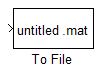
\includegraphics[width=0.5\textwidth]{Kapitel2/Bilder/image26}}
  \caption{Blockschaltbild eines linearen, zeitinvarianten Systems}
  \label{fig:ZeitinvarianzBSB}
\end{figure}

\noindent Die Direktstruktur ergibt sich unmittelbar aus der Differentialgleichung (\ref{eq:threehundredninetyfour}), die Koeffizienten an und b$_{m}$ entsprechen denen der Differentialgleichung. Bei dieser Darstellung ergibt sich das Problem, dass 2$\cdot$N Integrierer zur Systemrealisierung notwendig sind. Unter der Voraussetzung, dass das System ein lineares, zeitinvariantes System ist, ist eine Vertauschung der Funktionsblöcke möglich. Dieser
Sachverhalt wird nach der Beschreibung von LTI-Systemen im Laplace-Bereich noch einmal aufgegriffen. Nach Austauschen der Reihenfolge der Strukturen ergibt sich das in Bild \ref{fig:ZeitinvarianzBSBMitTausch} 3.27 dargestellte Blockschaltbild.

\begin{figure}[H]
  \centerline{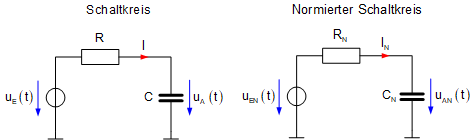
\includegraphics[width=0.5\textwidth]{Kapitel2/Bilder/image27}}
  \caption{Blockschaltbild eines linearen, zeitinvarianten Systems mit vertauschter Blockreihenfolge}
  \label{fig:ZeitinvarianzBSBMitTausch}
\end{figure}

\noindent Die beiden Pfade der Integrierer haben dieselben Eingangssignale, sie können ohne Veränderung derSystemfunktion zusammengefasst werden. Es ergibt sich das in Bild \ref{fig:KanonischZeitinvarianzBSB} dargestellte Blockschaltbild.

\begin{figure}[H]
  \centerline{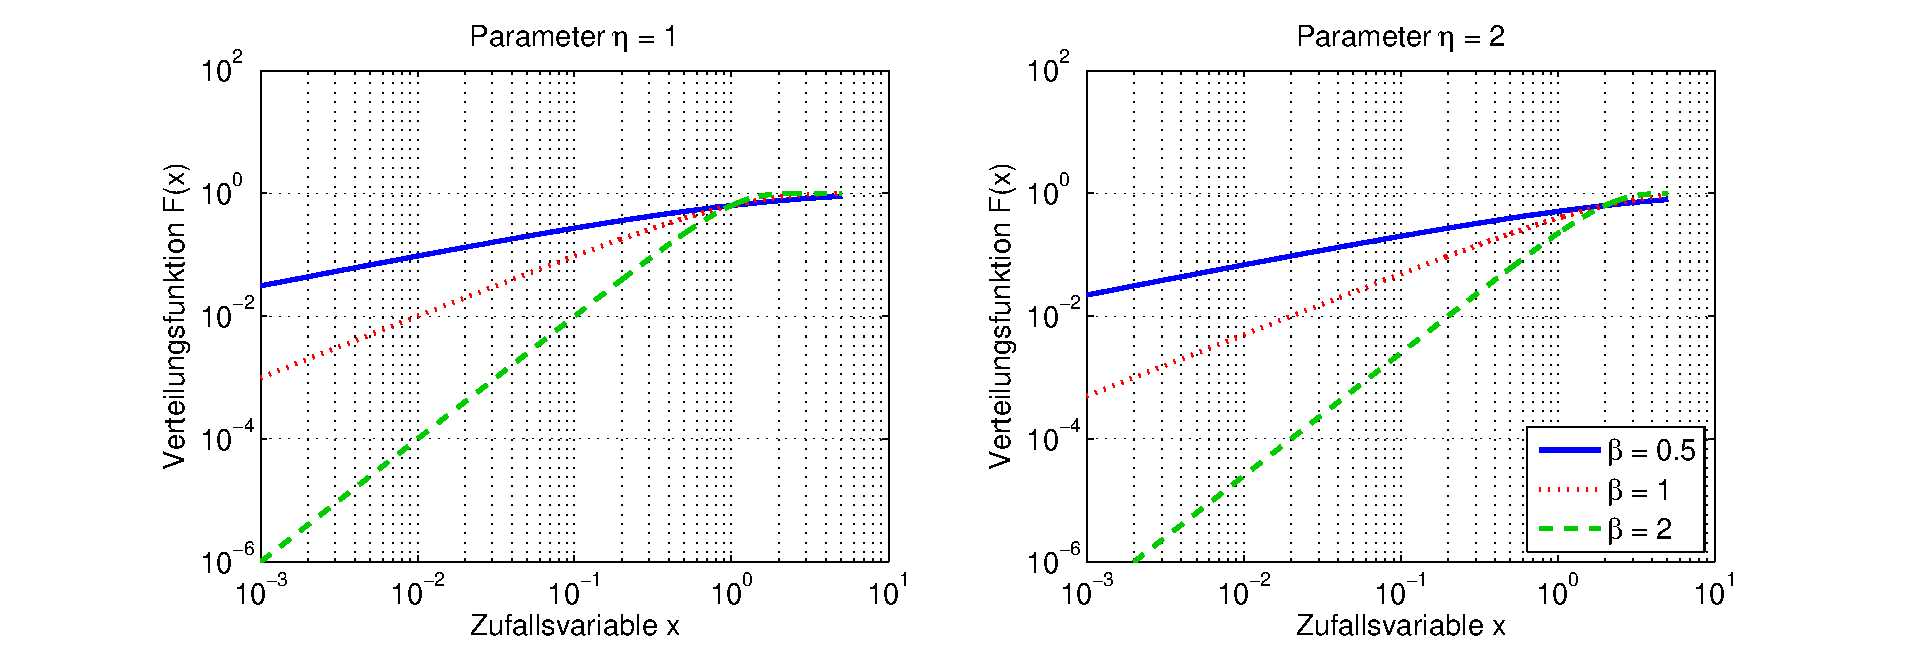
\includegraphics[width=0.5\textwidth]{Kapitel2/Bilder/image28}}
  \caption{Kanonisches Blockschaltbild eines linearen, zeitinvarianten Systems}
  \label{fig:KanonischZeitinvarianzBSB}
\end{figure}

\noindent Das System wird mit N Integrierern beschrieben. Es kann gezeigt werden, dass das System nicht mit weniger als N Integrierern realisiert werden kann. Die Darstellung wird deshalb als kanonisches Blockschaltbild bezeichnet.\bigskip

{\fontfamily{phv}\selectfont
\noindent\textbf{Mathematische motivierte Herleitung des Blockschaltbildes von LTI-Systemen}}

\noindent Auch die mathematisch orientierte Herleitung von Blockschaltbildern basiert auf der
Differentialgleichung

\begin{equation}\label{eq:threetwohundred}
a_{0}\cdot y(t) + a_{1}\cdot \frac{dy}{dt}+a_{2}\cdot \frac{d^2y}{dt^2}+ ... +a_{n}\cdot \frac{d^Ny}{dt^N}=
b_{0}\cdot u(t) + b_{1}\cdot \frac{du}{dt}+b_{2}\cdot \frac{d^2u}{dt^2}+ ... +b_{m}\cdot \frac{d^Mu}{dt^M}
\end{equation}

\noindent mit den entsprechenden Anfangsbedingungen. Das System kann in zwei Anteile zerlegt werden, die Eingangsgröße u(t) und ihre Ableitungen sowie die Ausgangsgröße y(t) und ihre Ableitungen. Die Gleichung kann in zwei Stufen aufgeteilt werden. Zunächst werden Linearkombinationen der Eingangsgröße und ihren Ableitungen gebildet.

\begin{equation}\label{eq:threetwohundredone}
x(t) = b_{0}\cdot u(t) + b_{1}\cdot \frac{du}{dt} +  b_{2}\cdot \frac{d^2u}{dt^2} + \cdots + b_{M}\cdot \frac{d^Mu}{dt^M}
\end{equation}

\noindent Anschließend wird eine Linearkombination der Ausgangsgröße y(t) und ihren Ableitungen berechnet und x(t) gleichgesetzt.

\begin{equation}\label{eq:threetwohundredtwo}
a_{0}\cdot y(t) + a_{1}\cdot \frac{dy}{dt}+a_{2}\cdot \frac{d^2y}{dt^2}+ ... +a_{n}\cdot \frac{d^Ny}{dt^N} = x(t)
\end{equation}

\noindent Grafisch sind diese Operationen in Bild 3.29 dargestellt.

\begin{figure}[H]
  \centerline{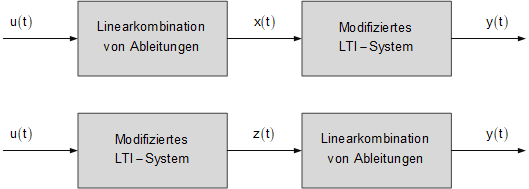
\includegraphics[width=0.5\textwidth]{Kapitel2/Bilder/image29}}
  \caption{Zerlegung eines Systems in zwei Teilsysteme bei variierter Reihenfolge der Funktionsblöcke}
  \label{fig:Zerlegung}
\end{figure}

\noindent Für das LTI-System ist die Reihenfolge der beiden Funktionsblöcke unerheblich, sodass die beiden Darstellungen in Bild \ref{fig:Zerlegung} äquivalent sind. Bei geänderter Reihenfolge gelten mit den Bezeichnungen in Bild \ref{fig:Zerlegung}  die Gleichungen

\begin{equation}\label{eq:threetwohundredthree}
a_{0}\cdot z(t) + a_{1}\cdot \frac{dz}{dt}+a_{2}\cdot \frac{d^2z}{dt^2}+ ... +a_{n}\cdot \frac{d^Nz}{dt^N} = u(t)
\end{equation}

\noindent und

\begin{equation}\label{eq:threetwohundredfour}
y(t) = b_{0}\cdot z(t) + b_{1}\cdot \frac{dz}{dt} + b_{2}\cdot \frac{d^2z}{dt^2} + \cdots + b_{M}\cdot \frac{d^Mz}{dt^M} 
\end{equation}

\noindent Die N-fache Integration von Gleichung (\ref{eq:threetwohundredthree})

\begin{equation}\label{eq:threetwohundredfive}
\begin{split}
& a_{0}\cdot \int\limits _{-\infty }^{t} \cdots  \int\limits _{-\infty }^{t_{3}}  \int\limits _{-\infty }^{t_{2}} z(\tau _{1}) d\tau _{1} d\tau _{2} \cdots d\tau _{N} + a_{1}\cdot \int\limits _{-\infty }^{t} \cdots  \int\limits _{-\infty }^{t_{3}}  \int\limits _{-\infty }^{t_{2}} z(\tau _{1}) d\tau _{1} d\tau _{2} \cdots d\tau _{N-1} + \cdots + a_{N} \cdot z(t)\\ 
& = \int\limits _{-\infty }^{t} \cdots  \int\limits _{-\infty }^{t_{3}} \int\limits _{-\infty }^{t_{2}} u(\tau _{1}) d\tau _{1} d\tau _{2} \cdots d\tau _{N}     
\end{split}
\end{equation}

\noindent und Auflösen nach z(t) führt zu dem Ausdruck

\begin{equation}\label{eq:threetwohundredsix}
\begin{split}
z(t) & = \frac{1}{a_{N}}\cdot  \int\limits _{-\infty }^{t} \cdots  \int\limits _{-\infty }^{\tau_{3}}  \int\limits _{-\infty }^{\tau_{2}} u(\tau _{1}) d\tau _{1} d\tau _{2} \cdots d\tau _{N} \\
 & - \frac{a_{0}}{a_{N}}\cdot\int\limits _{-\infty }^{t} \cdots  \int\limits _{-\infty }^{\tau_{3}}  \int\limits _{-\infty }^{\tau_{2}} z(\tau _{1}) d\tau _{1} d\tau _{2} \cdots d\tau _{N} - \cdots - \frac{a_{N-1}}{a_{N}}\cdot \int\limits _{-\infty }^{\tau_{2}} z(\tau _{N-1}) d\tau _{N-1}
\end{split}
\end{equation}	

\noindent Bild \ref{fig:BlockschaltbildTeilsystem} stellt diese Gleichung als Blockdiagramm dar.

\begin{figure}[H]
  \centerline{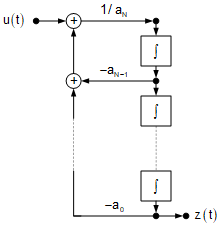
\includegraphics[width=0.4\textwidth]{Kapitel2/Bilder/image30}}
  \caption{Blockschaltbild des in Gleichung (\ref{eq:threetwohundredsix}) beschriebenen Teilsystems}
  \label{fig:BlockschaltbildTeilsystem}
\end{figure}

\noindent Das Ausgangssignal y(t) setzt sich nach Gleichung (\ref{eq:threetwohundredfour}) aus einer Linearkombination von Ableitungen der Größe z(t) zusammen.

\begin{equation}\label{eq:threetwohundredseven}
y(t) = b_{0}\cdot z(t) + b_{1}\cdot \frac{dz}{dt} + b_{2}\cdot \frac{d^2z}{dt^2} + \cdots + b_{M}\cdot \frac{d^Mz}{dt^M} 
\end{equation}

\noindent Die Eingangssignale der Integrierer sind Ableitungen der Größe z(t). Damit kann das Gesamtsystem mit dem Blockschaltbild in Bild (\ref{fig:BlockschaltbildZeitinvariant}) beschreiben werden.

\begin{figure}[H]
  \centerline{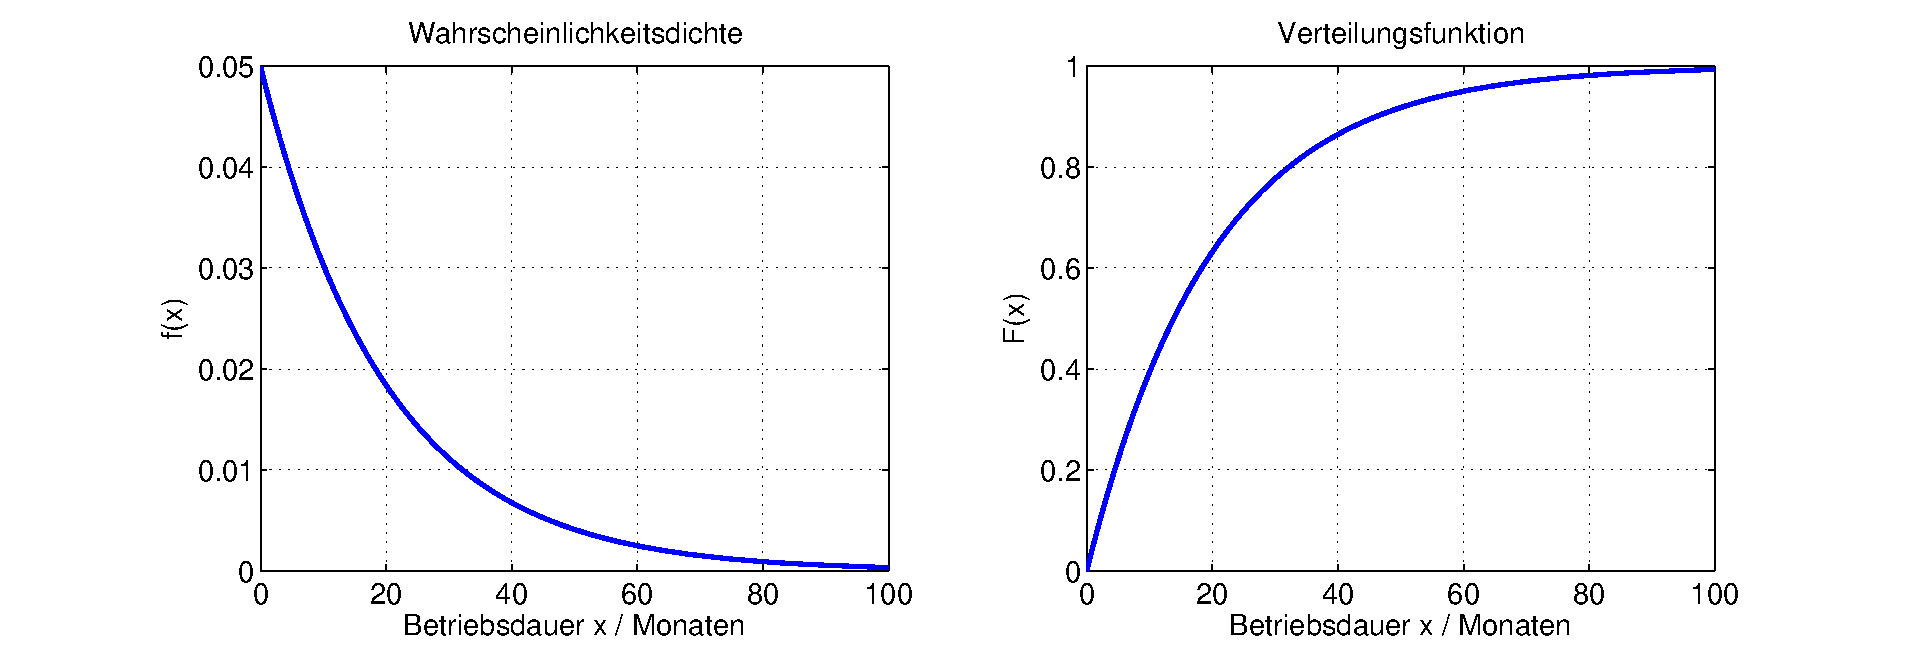
\includegraphics[width=0.7\textwidth]{Kapitel2/Bilder/image31}}
  \caption{Blockschaltbild eines linearen, zeitinvarianten Systems}
  \label{fig:BlockschaltbildZeitinvariant}
\end{figure}

\noindent In technischen Systemen gilt oftmals die Beziehung M < N, in diesem Fall sind die entsprechenden Koeffizienten b$_{m}$ zu null zu setzen.
Beide Herleitungen führen zu einem kanonischen Blockschaltbild mit N Integrierern. Bei der Integration müssen die Anfangsbedingungen in Form von \textit{Initial Conditions} berücksichtigt werden.

\bigskip

\noindent
\colorbox{lightgray}{%
\arrayrulecolor{white}%
\renewcommand\arraystretch{0.6}%
\begin{tabular}{ wl{16.5cm} }
{\fontfamily{phv}\selectfont
\noindent
Beispiel: Darstellung des Feder-Masse-Dämpfer-Systems als Blockschaltbild}
\end{tabular}%
}\bigskip

\noindent Die Anwendung der Systemdarstellung über Blockschaltbilder wird anhand eines Feder-Masse-
Dämpfer-Systems verdeutlicht.

\begin{equation}\label{eq:threetwohundredeight}
F_{E} \left(t\right)=m\cdot \frac{d^{2} x}{dt^{2} } +D\cdot \frac{dx}{dt} +c\cdot x\left(t\right)
\end{equation}

\noindent Eingangssignal ist der Kraftverlauf F$_{E}$(t), Ausgangssignal ist die Auslenkung x(t). Einsetzen der
entsprechenden Koeffizienten in die allgemeine Form führt zu der Darstellung des Systems als kanonisches Blockschaltbild. Es ist in Bild \ref{fig:BlockschaltbilFDM} dargestellt.

\begin{figure}[H]
  \centerline{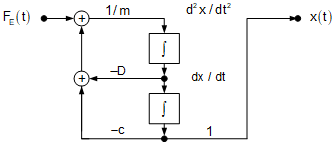
\includegraphics[width=0.5\textwidth]{Kapitel2/Bilder/image32}}
  \caption{Kanonisches Blockschaltbild eines Feder-Masse-Dämpfer-Systems}
  \label{fig:BlockschaltbilFDM}
\end{figure}

\noindent Diese Darstellung kann anschaulich interpretiert werden. Das Ausgangssignal des zweiten Integrierers ist die Auslenkung x(t) des Systems. Damit ist das Eingangssignal des zweiten Integrierers die erste Ableitung dx/dt und das Eingangssignal des ersten Integrierers die zweite Ableitung d²x/dt² der Auslenkung x(t). Nach Gleichung (\ref{eq:threetwohundredeight}) gilt für die zweite Ableitung

\begin{equation}\label{eq:threetwohundrednine}
\frac{d^{2} x}{dt^{2}} = \frac{1}{m} \cdot (F_{E}(t) - D\cdot \frac{dx}{dt} - c\cdot x\left(t\right))
\end{equation}

\noindent Eine Analyse des Signalflusses zeigt, dass das Blockschaltbild genau diese Struktur realisiert. Die
Anfangsbedingungen der beiden Integrierer ergeben sich aus x(t$_{0}$) und dx/dt an der Stelle t = t$_{0}$.

\subsubsection{Simulation von Systemen mit MATLAB / Simulink}

\noindent Das in Abschnitt \ref{threefiveone} beschriebene Blockschaltbild kann zur Simulation des Systems in Simulink verwendet werden. Dabei wird das Blockdiagramm in Simulink grafisch programmiert. Simulink stellt verschiedene elementare Übertragungsglieder zur Verfügung.\medskip

{\fontfamily{phv}\selectfont
\noindent\textbf{Signalquellen}}

\noindent Mithilfe von Signalquellen (\textit{Sources}) werden Eingangssignale generiert. Neben den typischen Signalformen wie Sprung-, Rampen-, Rechteck- und Sinusfunktion erlaubt Simulink die Erzeugung von Signalquellen über selbst definierte Variablen oder sogenannte mat-Files. Damit ist es zum Beispiel auch möglich, gemessene Daten als Signalquelle zu verwenden, indem die Messdaten aus mat-Files eingelesen werden. Tabelle \ref{tab:threeeleven} stellt eine Auswahl von Signalquellen in Simulink dar.

\clearpage

\begin{table}[H]
\caption{Auswahl von Signalquellen in Simulink}
\setlength{\fboxsep}{0pt}%
\colorbox{lightgray}{%
\arrayrulecolor{white}%
\begin{tabular}{| c | c | c | c |}
\hline
\parbox[c][0.28in][c]{1.6in}{\smallskip\centering\textbf{\fontfamily{phv}\selectfont{Signalquelle}}} & \parbox[c][0.28in][c]{1.5in}{\smallskip\centering\textbf{\fontfamily{phv}\selectfont{Simulink Symbol}}} &
\parbox[c][0.28in][c]{1.6in}{\smallskip\centering\textbf{\fontfamily{phv}\selectfont{Signalquelle}}} &
\parbox[c][0.28in][c]{1.5in}{\smallskip\centering\textbf{\fontfamily{phv}\selectfont{Simulink Symbol}}}\\ \hline


\parbox[c][0.9in][c]{1.6in}{\centering{\fontfamily{phv}\selectfont{Konstante}}} &
\parbox[c][0.9in][c]{1.5in}{\centerline{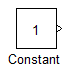
\includegraphics[width=0.1\textwidth]{Kapitel2/Table/image1.png}}} &
\parbox[c][0.9in][c]{1.6in}{\centering{\fontfamily{phv}\selectfont{Sinusfunktion}}} &
\parbox[c][0.9in][c]{1.5in}{\centerline{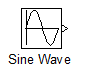
\includegraphics[width=0.1\textwidth]{Kapitel2/Table/image2.png}}} \\ \hline

\parbox[c][0.9in][c]{1.6in}{\centering{\fontfamily{phv}\selectfont{Sprungfunktion}}} &
\parbox[c][0.9in][c]{1.5in}{\centerline{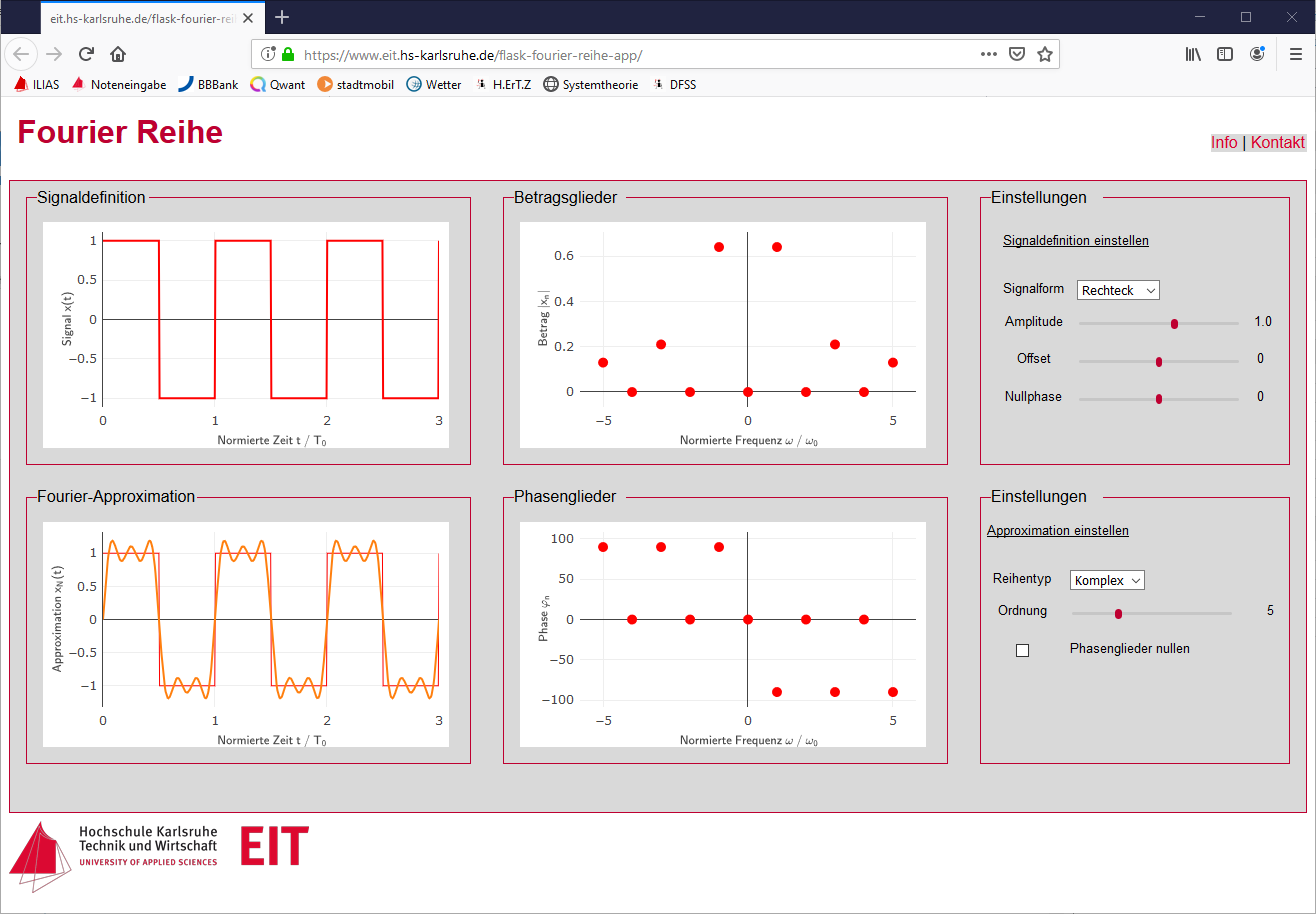
\includegraphics[width=0.085\textwidth]{Kapitel2/Table/image3.png}}}&
\parbox[c][0.9in][c]{1.6in}{\centering{\fontfamily{phv}\selectfont{Zugriff auf Variable im Workspace}}} &
\parbox[c][0.9in][c]{1.5in}{\centerline{\includegraphics[width=0.12\textwidth]{Kapitel2/Table/image4.png}}} \\ \hline

\parbox[c][0.9in][c]{1.6in}{\centering{\fontfamily{phv}\selectfont{Rampenfunktion}}} &
\parbox[c][0.9in][c]{1.5in}{\centerline{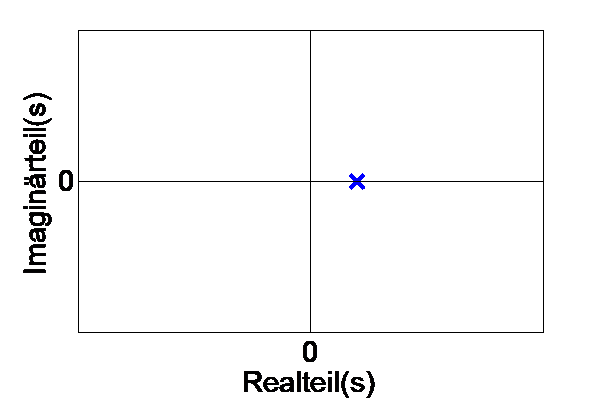
\includegraphics[width=0.085\textwidth]{Kapitel2/Table/image5.png}}} &
\parbox[c][0.9in][c]{1.6in}{\centering{\fontfamily{phv}\selectfont{Definition in mat-File}}} &
\parbox[c][0.9in][c]{1.5in}{\centerline{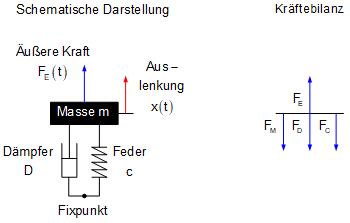
\includegraphics[width=0.12\textwidth]{Kapitel2/Table/image6.png}}} \\ \hline

\parbox[c][0.9in][c]{1.6in}{\centering{\fontfamily{phv}\selectfont{Rechteckfunktion}}} &
\parbox[c][0.9in][c]{1.5in}{\centerline{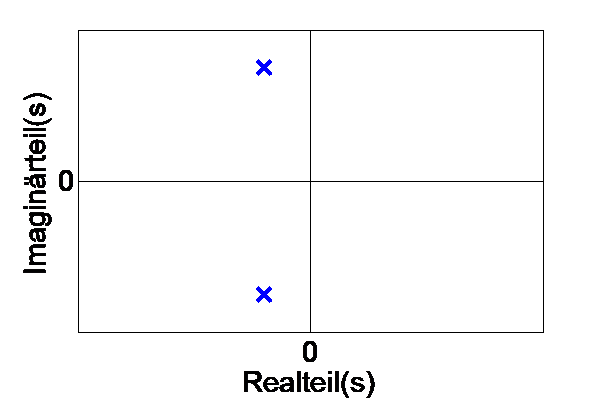
\includegraphics[width=0.1\textwidth]{Kapitel2/Table/image7.png}}} &
\parbox[c][0.9in][c]{1.6in}{\centering{\fontfamily{phv}\selectfont{Zeit}}} &
\parbox[c][0.9in][c]{1.5in}{\centerline{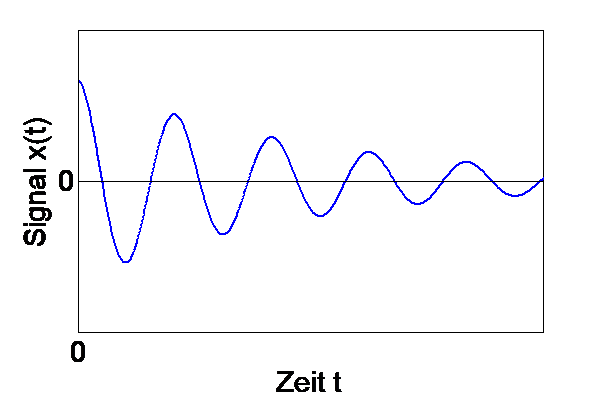
\includegraphics[width=0.07\textwidth]{Kapitel2/Table/image8.png}}}\\ \hline

\end{tabular}%
}\bigskip
\label{tab:threeeleven}
\end{table}

\medskip

{\fontfamily{phv}\selectfont
\noindent\textbf{Signalpfade und Verknüpfung von Signalpfaden}}

\noindent Simulink definiert Systeme über das Verbinden von Funktionsblöcken mit Signalpfaden. Zum Beispiel könnte ein System, das die Gleichung

\begin{equation}\label{eq:threetwohundredten}
y(t) = 3 \cdot u(t) + 1
\end{equation}

\noindent erfüllt, in Simulink über das Modell in Bild \ref{fig:SimulinkModell} dargestellt werden. Dabei wird u(t) als Signalquelle mit Sinusfunktion realisiert.

\begin{figure}[H]
  \centerline{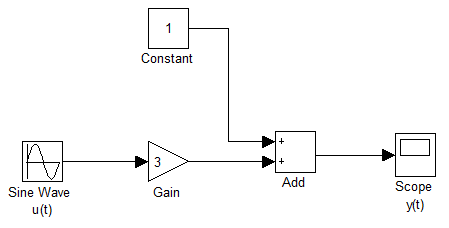
\includegraphics[width=0.5\textwidth]{Kapitel2/Bilder/image33}}
  \caption{Einfaches Simulink Modell}
  \label{fig:SimulinkModell}
\end{figure}

\noindent Die Signalpfade laufen durch Blöcke, die eine definierte Funktion ausführen. Diese Funktion kann neben Additionen, Subtraktion, Multiplikation und Division auch eine höhere mathematische Funktion sein, die als \textit{Math-Function-Block} definiert wird. Mit den Blöcken Multiplexer und Demultiplexer können Signale zu einem mehrdimensionalen Signalpfad zusammengefasst beziehungsweise von einem Signalpfad in einzelne Signale zerlegt werden. Tabelle \ref{tab:threetwelve} stellt eine Auswahl von Verknüpfungen in Simulink dar.

\clearpage
\begin{table}[H]
\caption{Auswahl von Funktionen zur Signalverknüpfung}
\setlength{\fboxsep}{0pt}%
\colorbox{lightgray}{%
\arrayrulecolor{white}%
\begin{tabular}{| c | c | c | c |}
\hline
\parbox[c][0.28in][c]{1.6in}{\smallskip\centering\textbf{\fontfamily{phv}\selectfont{Operation}}} & \parbox[c][0.28in][c]{1.5in}{\smallskip\centering\textbf{\fontfamily{phv}\selectfont{Simulink Symbol}}} &
\parbox[c][0.28in][c]{1.6in}{\smallskip\centering\textbf{\fontfamily{phv}\selectfont{Operation}}} &
\parbox[c][0.28in][c]{1.5in}{\smallskip\centering\textbf{\fontfamily{phv}\selectfont{Simulink Symbol}}}\\ \hline


\parbox[c][0.9in][c]{1.6in}{\centering{\fontfamily{phv}\selectfont{Addition von Signalen}}} &
\parbox[c][0.9in][c]{1.5in}{\centerline{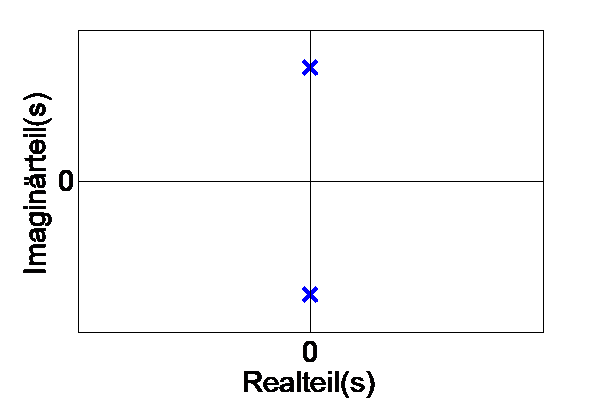
\includegraphics[width=0.1\textwidth]{Kapitel2/Table/image9.png}}} &
\parbox[c][0.9in][c]{1.6in}{\centering{\fontfamily{phv}\selectfont{Multiplikation / Division \\ von Signalen}}} &
\parbox[c][0.9in][c]{1.5in}{\centerline{\includegraphics[width=0.1\textwidth]{Kapitel2/Table/image10.png}}} \\ \hline

\parbox[c][0.9in][c]{1.6in}{\centering{\fontfamily{phv}\selectfont{Multiplikation \\
mit einem Faktor, \\
Verstärkung}}} &
\parbox[c][0.9in][c]{1.5in}{\centerline{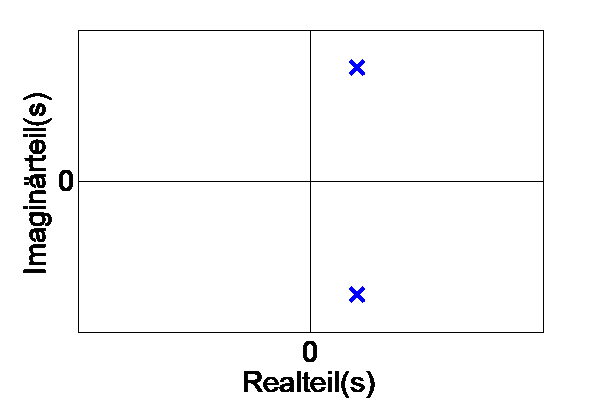
\includegraphics[width=0.1\textwidth]{Kapitel2/Table/image11.png}}} &
\parbox[c][0.9in][c]{1.6in}{\centering{\fontfamily{phv}\selectfont{Mathematische \\
Funktionen}}} &
\parbox[c][0.9in][c]{1.5in}{\centerline{\includegraphics[width=0.1\textwidth]{Kapitel2/Table/image12.png}}} \\ \hline

\parbox[c][0.9in][c]{1.6in}{\centering{\fontfamily{phv}\selectfont{Multiplexer}}} &
\parbox[c][0.9in][c]{1.5in}{\centerline{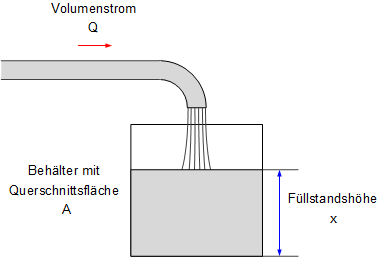
\includegraphics[width=0.05\textwidth]{Kapitel2/Table/image13.png}}} &
\parbox[c][0.9in][c]{1.6in}{\centering{\fontfamily{phv}\selectfont{Demultiplexer}}} &
\parbox[c][0.9in][c]{1.5in}{\centerline{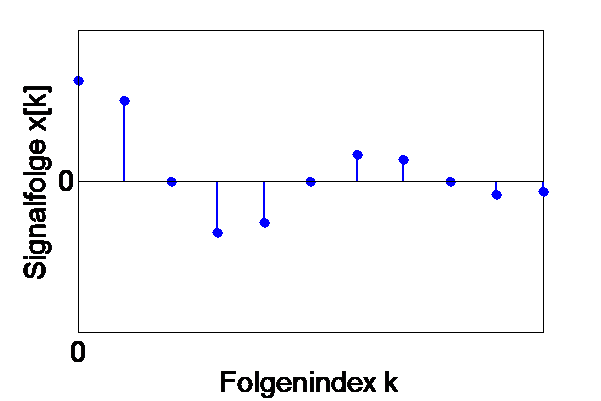
\includegraphics[width=0.05\textwidth]{Kapitel2/Table/image14.png}}} \\ \hline 

\end{tabular}%
}\bigskip
\label{tab:threetwelve}
\end{table}

{\fontfamily{phv}\selectfont
\noindent\textbf{Elementare Übertragungsglieder}}

\noindent Tabelle \ref{tab:threethirteen} zeigt die elementaren Übertragungsglieder zur Darstellung eines linearen, zeitinvarianten Systems als Blockschaltbild.

\begin{table}[H]
\caption{Elementare Übertragungsglieder in Simulink}
\setlength{\fboxsep}{0pt}%
\colorbox{lightgray}{%
\arrayrulecolor{white}%
\begin{tabular}{| c | c | c | c |}
\hline
\parbox[c][0.28in][c]{1.6in}{\smallskip\centering\textbf{\fontfamily{phv}\selectfont{Übertragungsfunktion}}} & \parbox[c][0.28in][c]{1.5in}{\smallskip\centering\textbf{\fontfamily{phv}\selectfont{Simulink Symbol}}} &
\parbox[c][0.28in][c]{1.6in}{\smallskip\centering\textbf{\fontfamily{phv}\selectfont{Übertragungsfunktion}}} &
\parbox[c][0.28in][c]{1.5in}{\smallskip\centering\textbf{\fontfamily{phv}\selectfont{Simulink Symbol}}}\\ \hline

\parbox[c][0.9in][c]{1.6in}{\centering{\fontfamily{phv}\selectfont{Integration}}} &
\parbox[c][0.9in][c]{1.5in}{\centerline{\includegraphics[width=0.1\textwidth]{Kapitel2/Table/image15.png}}} &
\parbox[c][0.9in][c]{1.6in}{\centering{\fontfamily{phv}\selectfont{Differentiation}}} &
\parbox[c][0.9in][c]{1.5in}{\centerline{\includegraphics[width=0.1\textwidth]{Kapitel2/Table/image16.png}}} \\ \hline

\end{tabular}%
}\bigskip
\label{tab:threethirteen}
\end{table}

\noindent Integrierer besitzen das Symbol 1/s, im Laplace-Bereich ist das die Übertragungsfunktion eines Integrierers. Durch ein doppeltes Klicken auf die Symbole öffnet sich in Simulink ein Dialog, mit dem die Eigenschaften des Übertragungsglieds definiert werden können. Insbesondere kann bei Integrierern die Anfangsbedingung (\textit{Initial Condition}) festgelegt werden. Wird kein spezieller Anfangswert definiert, verwendet Simulink den Anfangswert y(0) = 0.
\clearpage
\begin{figure}[H]
  \centerline{\includegraphics[width=0.5\textwidth]{Kapitel2/Bilder/image34}}
  \caption{Dialog zur Definition der Eigenschaften eines Integrierers, insbesondere der Anfangsbedingung}
  \label{fig:DialogAnfangsbedingung}
\end{figure}

\noindent Differenzierer sind an dem Symbol du/dt zu erkennen, was auf die zeitliche Ableitung der Eingangsgröße hinweist. Zu Beginn des Abschnitts wird darauf hingewiesen, dass die numerische Realisierung kritisch ist, die Differentiation nicht kausal ist und zu einer Verstärkung von Rauschanteilen im Signal führt. Deshalb sollte auf den Einsatz von Differenzierern verzichtet werden.
Neben den elementaren Übertragungsgliedern Integrierer oder Differenzierer bietet Simulink die Möglichkeit, komplexere Übertragungsglieder im Laplace-Bereich zu definieren. Diese Darstellungsform wird nach der Beschreibung von Systemen im Laplace-Bereich aufgegriffen.

\medskip

{\fontfamily{phv}\selectfont
\noindent\textbf{Signalsenken}}

\noindent Die in Simulink berechneten Signalpfade enden in sogenannten Signalsenken (\textit{Sinks}). Signalsenken stellen das Signal grafisch dar oder speichern das Signal in Variablen oder mat-Files. Tabelle \ref{tab:threefourteen} stellt eine Auswahl von Signalsenken in Simulink dar.

\clearpage

\begin{table}[H]
\caption{Auswahl von Signalsenken in Simulink}
\setlength{\fboxsep}{0pt}%
\colorbox{lightgray}{%
\arrayrulecolor{white}%
\begin{tabular}{| c | c | c | c |}
\hline
\parbox[c][0.28in][c]{1.6in}{\smallskip\centering\textbf{\fontfamily{phv}\selectfont{Signalsenke}}} & \parbox[c][0.28in][c]{1.5in}{\smallskip\centering\textbf{\fontfamily{phv}\selectfont{Simulink Symbol}}} &
\parbox[c][0.28in][c]{1.6in}{\smallskip\centering\textbf{\fontfamily{phv}\selectfont{Signalsenke}}} &
\parbox[c][0.28in][c]{1.5in}{\smallskip\centering\textbf{\fontfamily{phv}\selectfont{Simulink Symbol}}}\\ \hline


\parbox[c][0.9in][c]{1.6in}{\centering{\fontfamily{phv}\selectfont{Numerische Anzeige}}} &
\parbox[c][0.9in][c]{1.5in}{\centerline{\includegraphics[width=0.14\textwidth]{Kapitel2/Table/image17.png}}}  &
\parbox[c][0.9in][c]{1.6in}{\centering{\fontfamily{phv}\selectfont{Grafische Darstellung}}} &
\parbox[c][0.9in][c]{1.5in}{\centerline{\includegraphics[width=0.08\textwidth]{Kapitel2/Table/image18.png}}}\\ \hline

\parbox[c][0.9in][c]{1.2in}{\centering{\fontfamily{phv}\selectfont{Speicherung in Variable im Workspace}}} &
\parbox[c][0.9in][c]{1.5in}{\centerline{\includegraphics[width=0.12\textwidth]{Kapitel2/Table/image19.png}}} &
\parbox[c][0.9in][c]{1.2in}{\centering{\fontfamily{phv}\selectfont{Speicherung in mat-File}}} &
\parbox[c][0.9in][c]{1.5in}{\centerline{\includegraphics[width=0.12\textwidth]{Kapitel2/Table/image20.png}}} \\ \hline

\end{tabular}%
}\bigskip
\label{tab:threefourteen}
\end{table}
\medskip

{\fontfamily{phv}\selectfont
\noindent\textbf{Simulationsvarianten zeitkontinuierlicher Systeme}}\smallskip

\noindent Zeitkontinuierliche Systeme werden in Simulink typischerweise als Variable-Step-Simulation ausgeführt. Dabei bestimmt Simulink auf Basis der Simulationsergebnisse eine variable Schrittweite, die bei vorgegebener Toleranz zu einer minimalen Rechenzeit führt. Die Simulation wird in einem Fenster vorgenommen, das über den Menüpunkt \textit{Simulation / Configuration}  Parameters aufgerufen wird. Es erscheint das Fenster, das in Bild \ref{fig:SimulinkParameters} dargestellt ist.

\begin{figure}[H]
  \centerline{\includegraphics[width=1\textwidth]{Kapitel2/Bilder/image35}}
  \caption{Fenster zur Konfiguration von Parametern in Simulink}
  \label{fig:SimulinkParameters}
\end{figure}

\noindent Für die Simulation sind neben Start- und Endzeitpunkt die Solver-Optionen von Bedeutung. Informationen zu den Eigenschaften der Solver und ihren Anwendungsgebieten sind in [Schw07] und [Stei07] zu finden. Im Rahmen der Vorlesung werden die Simulationen mit dem Solver \textit{ode45 (Dormand-Prince)} ausgeführt. Alle Default-Einstellungen von Simulink werden übernommen.\bigskip

\noindent
\colorbox{lightgray}{%
\arrayrulecolor{white}%
\renewcommand\arraystretch{0.6}%
\begin{tabular}{ wl{16.5cm} }
{\fontfamily{phv}\selectfont
\noindent
Beispiel: Simulation eines Feder-Masse-Dämpfer-Systems}
\end{tabular}%
}\bigskip

\noindent Zur Simulation eines Feder-Masse-Dämpfer-Systems wird das hergeleitete Blockschaltbild mithilfe der
mathematischen Funktionen sowie der Integrierer in MATLAB dargestellt. Es ergibt sich das in Bild \ref{fig:FMDinSimulink} dargestellte Simulink-Modell.

\begin{figure}[H]
  \centerline{\includegraphics[width=0.6\textwidth]{Kapitel2/Bilder/image36}}
  \caption{Blockschaltbild eines Feder-Masse-Dämpfer-Systems in Simulink }
  \label{fig:FMDinSimulink}
\end{figure}

\noindent Als Signalquelle wird eine Sprungfunktion eingesetzt. Ein- und Ausgangssignal werden in einem sogenannten \textit{Scope}  dargestellt. Für eine Federkonstante von c = 100 N/m, eine Dämpfung von D = 0.5 N$\cdot$s/m, eine Masse m = 10 g und eine Kraft F0 = 0.2 N ergibt sich das in Bild \ref{fig:SimulationFDM} \textit{Scope}-Bild.

\begin{figure}[H]
  \centerline{\includegraphics[width=0.5\textwidth]{Kapitel2/Bilder/image37}}
  \caption{Simulation des Einschwingverhaltens des Feder-Masse-Dämpfer-Systems bei einer sprungförmigen Anre-gung mit einer Kraft von 0.2 N dargestellt als Scope in Simulink}
  \label{fig:SimulationFDM}
\end{figure}

\noindent Das Eingangssignal ist in dem oberen Feld als Sprung zu erkennen. Das Ausgangssignal ist im unteren Feld dargestellt. Das Simulationsergebnis entspricht dem in Bild \ref{fig:SimulationFDM} dargestellten Signalverlauf.

\clearpage

\subsection{Literatur}


\subsubsection{Literaturstellen mit anschaulicher Darstellung}

\begin{tabular}{|p{0.6in}|p{5.7in}|} \hline 
[Alba04] & Albach, Manfred: Grundlagen der Elektrotechnik 1und 2.\\ 
& Pearson Studium, 2004 \\ \hline 
[Foel11] & Föllinger, Otto: Laplace-, Fourier- und z-Transformation. 10., überarbeitete Auflage \\ 
& VDE Verlag GmbH, Berlin, Offenbach 2011 \\ \hline 
[Führ06] & Führer, Arnold: Grundgebiete der Elektrotechnik 1 - 3 \\
& Hanser Verlag, München, 2006\\ \hline 
[Goeb11] & Goebbels, Steffen: Mathematik verstehen und anwenden \\
& Spektrum Akademischer Verlag, Heidelberg, 2011 \\ \hline 
[Papu01] & Papula, Lothar: Mathematik für Ingenieure und Naturwissenschaftler \\
& Vieweg Fachbücher der Technik, Braunschweig/Wiesbaden, 2001 \\ \hline 
\end{tabular}


\subsubsection{Literatur zu MATLAB}

\begin{tabular}{|p{0.6in}|p{5.7in}|} \hline 
[Beuc00] & Beucher, Ottmar: MATLAB und Simulink lernen,\\
& Addison Wesley Longman Verlag, München, 2000\\ \hline 
[Schw07] & Schweizer, Wolfgang: MATLAB kompakt, \\ 
& Oldenbourg Verlag München, 2007\\ \hline 
[Stei07] & Stein, Ulrich: Einstieg in das Programmieren mit MATLAB,\\
& Fachbuchverlag Leipzig, 2007\\ \hline 
\end{tabular}


\subsubsection{Literaturstellen mit praktischen Anwendungen mit MATLAB}

\begin{tabular}{|p{0.6in}|p{5.7in}|} \hline 
[Hoff98] & Hoffmann, Josef: Matlab und Simulink, \\
& Addison Wesley Longman Verlag, München, 1998\\ \hline 
[Hoff99] & Hoffmann, Josef: Matlab und Simulink in der Signalverarbeitung und \\
& Kommunikationstechnik, Addison Wesley Longman Verlag, München, 1999\\ \hline 
[Sche04] & Scherf, Helmut: Modellbildung und Simulation dynamischer Systeme,\\
& Oldenbourg Verlag, München, 2004\\ \hline 
\end{tabular}


\subsubsection{Weiterführende Literatur}

\begin{tabular}{|p{0.6in}|p{5.7in}|} \hline 
[Bart89] & Barton, G.: Elements of Green's Functions and Propagation: Potentials, Diffusion, and\\
&   Waves, Oxford University Press, 1989\\ \hline 
\end{tabular}

\clearpage

\section{Beschreibende Statistik univariater Daten}\label{three}
\noindent Zeitkontinuierliche Signale können mithilfe der Laplace-Transformation in einen sogenannten Laplace-
Bereich transformiert werden. Im Laplace-Bereich lassen sich lineare Differentialgleichungen mit konstanten Koeffizienten vergleichsweise einfach und anschaulich lösen. Rechenregeln der Laplace- Transformation erlauben eine vergleichsweise einfache Behandlung der Anfangsbedingungen. Darüber hinaus eignet sich der Laplace-Bereich zur Charakterisierung von linearen, zeitinvarianten Systemen mit sogenannten Übertragungsfunktionen.\newline

\noindent In diesem Kapitel wird die Laplace-Transformation vorgestellt. Nach der Definition der Laplace-Transformation werden einige Korrespondenzen über die Definitionsgleichung bestimmt. Die eher aufwendige Bestimmung von Korrespondenzen über die Definitionsgleichung kann vermieden werden, wenn die vorliegende Funktion auf Funktionen mit bekannten Korrespondenzen zurückgeführt werden kann. Die dazu notwendigen Rechenregeln werden hergeleitet und der Nutzen an Beispielen demonstriert.\newline

\noindent Anhand eines einfachen Beispiels wird die Bedeutung der Laplace-Transformation für die Lösung von
Differentialgleichungen aufgezeigt. Dabei wird motiviert, warum die Rücktransformation vom Laplace- Bereich in den Zeitbereich erforderlich ist. Die Rücktransformation vom Laplace-Bereich in den Zeitbereich kann grundsätzlich über ein Umkehrintegral erfolgen. Da dieser Weg aufwendig ist und Kenntnisse in der Funktionentheorie voraussetzt, wird er in der Praxis vermieden. Die bei technischen
Anwendungen entstehenden Laplace-Transformierten sind typischerweise gebrochen rationale Funktionen. Sie können in Partialbrüche zerlegt werden, die sich mithilfe der angesprochenen Rechenregeln und einiger Korrespondenzen in den Zeitbereich transformieren lassen.\newline

\noindent Die computerunterstützte Berechnung von Laplace-Transformierten wird anhand des Programms MATLAB beschrieben. Nach der Zusammenstellung der für die analytische Berechnung wesentlichen Befehle werden einige Beispiele und Beweise mithilfe der \textit{Symbolic Math Toolbox} berechnet.

\subsection{Grundlagen der Laplace-Transformation}

\subsubsection{Definitionsgleichung der Laplace-Transformation}\label{threeoneone}

\noindent Für kausale Signale ist die einseitige Laplace-Transformation definiert als

\begin{equation}\label{eq:fourone}
X(s) = \int\limits _{0}^{\infty} x(t) \cdot e^{-s\cdot t} dt
\end{equation}

\noindent Dabei ist s eine komplexe Zahl mit Realteil und Imaginärteil. Das Integral startet dabei an der Stelle t = 0-. Damit schließt das Laplace-Integral in Gleichung (\ref{eq:fourone}) Singularitäten an der Stelle t = 0 mit ein.
Es wird sich zeigen, dass daraus ein Formalismus entsteht, mit dem Übergangsbedingungen elegant bestimmt werden können. Die Transformation wird mit einem großen $L$ symbolisiert.

\begin{equation}\label{eq:fourtwo}
L\left\{x\left(t\right)\right\}=X\left(s\right)=\int\limits _{0_{-} }^{\infty }x\left(t\right)\cdot e^{-s\cdot t} {\rm \; } dt
\end{equation}

\noindent Ein Paar aus Zeitfunktion x(t) und Laplace-Transformierter X(s) wird auch als Korrespondenz bezeichnet. Korrespondenzen werden in der Literatur mit einem halb ausgef\"{u}llten Hantelzeichen dargestellt. Die nicht ausgef\"{u}llte Seite repr\"{a}sentiert dabei den Zeitbereich, die ausgef\"{u}llte Seite den transformierten Bereich.

\begin{equation}\label{eq:fourthree}
x\left(t\right)\circ -\bullet X\left(s\right)
\end{equation}


\noindent Die Laplace-Transformation bildet demnach Zeitfunktionen x(t) auf ihre Laplace-Transformierte X(s) ab. Die Variable s ist eine komplexe Variable. Die zugehörige komplexe Ebene wird auch als s-Ebene bezeichnet. Eine wichtige Eigenschaft der Laplace-Transformation besteht darin, dass der Differentiation und Integration im Zeitbereich einfache algebraische Operationen im Laplace-Bereich entsprechen. Au{\ss}erdem geht eine Faltung im Zeitbereich in eine Multiplikation im Laplace-Bereich \"{u}ber. Diese und andere Eigenschaften werden in Abschnitt 4.2 hergeleitet.

\subsubsection{Laplace-Transformation grundlegender Signale}
\noindent Zur Einführung werden die Laplace-Transformierten von einigen kausalen Funktionen über die Definitionsgleichung der Laplace-Transformation berechnet. Dabei ist zu berücksichtigen, dass im Rahmen dieser Buchreihe die einseitige Laplace-Transformation durchgeführt wird, die nur für kausale Signale definiert ist.\medskip

{\fontfamily{phv}\selectfont
\noindent\textbf{Kausale Rechteckfunktion}}\smallskip

\noindent Eine Rechteckfunktion mit der Gleichung

\begin{equation}\label{eq:fourfour}
x\left(t\right)=\sigma \left(t\right)-\sigma \left(t-t_{0} \right)
\end{equation}

\noindent soll in den Laplace-Bereich transformiert werden. Das Signal ist in Bild \ref{fig:LaplaceSignaleRechteck} dargestellt.

\begin{figure}[H]
  \centerline{\includegraphics[width=0.5\textwidth]{Kapitel3/Bilder/image1}}
  \caption{Kausale Rechteckfunktion x(t)}
  \label{fig:LaplaceSignaleRechteck}
\end{figure}

\noindent Einsetzen der Zeitfunktion x(t) in die Definitionsgleichung führt zu

\begin{equation}\label{eq:fourfive}
X\left(s\right)=\int\limits _{0_{-} }^{\infty }x\left(t\right)\cdot e^{-s\cdot t} {\rm \; } dt=\int\limits _{0_{-} }^{\infty }\left(\sigma \left(t\right)-\sigma \left(t-t_{0} \right)\right)\cdot e^{-s\cdot t} {\rm \; } dt
\end{equation}

\noindent Die kausale Rechteckfunktion ist nur in dem Bereich von 0${}_{-}$ bis t${}_{0}$ von null verschieden. Damit muss auch die Integration nur in diesem Bereich durchgef\"{u}hrt werden. In dem Bereich ist die Funktion x(t) konstant gleich 1. Damit kann das Integral umgeformt werden zu

\begin{equation}\label{eq:foursix}
X\left(s\right)=\int\limits _{0_{-} }^{\infty }\left(\sigma \left(t\right)-\sigma \left(t-t_{0} \right)\right)\cdot e^{-s\cdot t} {\rm \; } dt=\int\limits _{0_{-} }^{t_{0} }1\cdot e^{-s\cdot t} {\rm \; } dt
\end{equation}

\noindent Mit der Stammfunktion der Exponentialfunktion

\begin{equation}\label{eq:fourseven}
\int\limits e^{a\cdot t} {\rm \; dt} =\frac{1}{a} \cdot e^{a\cdot t}
\end{equation}

\noindent und durch Einsetzen der Integrationsgrenzen ergibt sich die Laplace-Transformierte

\begin{equation}\label{eq:foureight}
X\left(s\right)=\int\limits _{0_{-} }^{t_{0} }1\cdot e^{-s\cdot t} {\rm \; } dt=\left. -\frac{1}{s} \cdot e^{-s\cdot t} \right|_{0_{-} }^{t_{0} } =-\frac{1}{s} \cdot e^{-s\cdot t_{0} } +\frac{1}{s} \cdot e^{-s\cdot 0_{-} } =\frac{1}{s} \cdot \left(1-e^{-s\cdot t_{0} } \right)
\end{equation}
\medskip

{\fontfamily{phv}\selectfont
\noindent\textbf{Impulsfunktion}}\smallskip

\noindent Als weiteres Beispiel werden die Laplace-Transformierten einer Impulsfunktion x$_{1}$(t) und einer verschobenen Impulsfunktion x$_{2}$(t) berechnet. 

\begin{equation}\label{eq:fournine}
x_{1} \left(t\right)=\delta \left(t\right)
\end{equation}

\begin{equation}\label{eq:fourten}
x_{2} \left(t\right)=\delta \left(t-t_{0} \right)
\end{equation}

\noindent Die beiden Signale sind in Bild \ref{fig:LaplaceSignaleImpuls} dargestellt.

\begin{figure}[H]
  \centerline{\includegraphics[width=1\textwidth]{Kapitel3/Bilder/image2}}
  \caption{Impulsfunktion x$_{1}$(t) und verschobene Impulsfunktion x$_{2}$(t)}
  \label{fig:LaplaceSignaleImpuls}
\end{figure}

\noindent Einsetzen der Impulsfunktion in die Definitionsgleichung f\"{u}hrt mit der Ausblendeigenschaft der Impulsfunktion zu

\begin{equation}\label{eq:foureleven}
X_{1} \left(s\right)=\int\limits _{0_{-} }^{\infty }\delta \left(t\right)\cdot e^{-s\cdot t} {\rm \; } dt=e^{-s\cdot 0} \cdot \int\limits _{0_{-} }^{\infty }\delta \left(t\right){\rm \; } dt=1\cdot \int\limits _{0_{-} }^{\infty }\delta \left(t\right){\rm \; } dt=1
\end{equation}

\noindent Analog ergibt sich f\"{u}r den verschobenen Impuls die Laplace-Transformierte 

\begin{equation}\label{eq:fourtwelve}
X_{2} \left(s\right)=\int _{0_{-} }^{\infty }\delta \left(t-t_{0} \right)\cdot e^{-s\cdot t} {\rm \; } dt=e^{-s\cdot t_{0} } \cdot \int _{0_{-} }^{\infty }\delta \left(t-t_{0} \right){\rm \; } dt=e^{-s\cdot t_{0} }
\end{equation}

\noindent Die Impulsfunktion $\delta$(t) besitzt die Laplace-Transformierte X(s) = 1. Eine Verschiebung des Impulses um t$_{0}$ nach rechts führt zu der Laplace-Transformierten e$^{-s\cdot t_{0}}$. In Abschnitt 4.2 wird sich zeigen, dass eine Verschiebung der Zeitfunktion um t$_{0}$ nach rechts immer zu einer Multiplikation mit dem Faktor e$^{-s\cdot t_{0}}$ führt.\bigskip

{\fontfamily{phv}\selectfont
\noindent\textbf{Sprungfunktion}}\smallskip

\noindent Die Sprungfunktion $\sigma$(t) springt zum Zeitpunkt t = 0 von null auf den Wert eins. Sie ist in Bild \ref{fig:LaplaceSignaleSprung} dargestellt.

\begin{figure}[H]
  \centerline{\includegraphics[width=0.5\textwidth]{Kapitel3/Bilder/image3}}
  \caption{Sprungfunktion $\sigma$}
  \label{fig:LaplaceSignaleSprung}
\end{figure}

\begin{equation}\label{eq:fourthirteen}
X\left(s\right)=\int\limits _{0_{-} }^{\infty }\sigma \left(t\right)\cdot e^{-s\cdot t} \;dt=\int\limits _{0_{-} }^{\infty }1\cdot e^{-s\cdot t} \;dt=\int\limits _{0_{-} }^{\infty }e^{-s\cdot t}\; dt
\end{equation}

\noindent Da die Sprungfunktion zeitlich nicht begrenzt ist, weist das Integral einen unendlich langen Integrationsbereich auf. Derartige Integrale werden uneigentliche Integrale genannt. Bilden der Stammfunktion und Einsetzen der Integrationsgrenzen führen zu dem Ausdruck

\begin{equation}\label{eq:fourfourteen}
X\left(s\right)=\left. -\frac{1}{s} \cdot e^{-s\cdot t} \right|_{0_{-} }^{\infty } =-\lim \limits_{t\to \infty } \frac{1}{s} \cdot e^{-s\cdot t} +\frac{1}{s} \cdot e^{-s\cdot 0_{-} } =\frac{1}{s} \cdot \left(1-\lim \limits_{t\to \infty } e^{-s\cdot t} \right)
\end{equation}

\noindent Dabei ist die Zahl s eine komplexe Zahl s = $\delta$ + j$\cdot\omega$. Der Grenzwert existiert nur, wenn der Realteil $\delta$ der komplexen Zahl s positiv ist. In diesem Fall gilt

\begin{equation}\label{eq:fourfifteen}
X\left(s\right)=\frac{1}{s} \cdot \left(1-\lim\limits_{t\to \infty} e^{-s\cdot t} \right)=\frac{1}{s} \cdot \left(1-\lim\limits_{t\to \infty } e^{-\left(\delta +j\cdot \omega \right)\cdot t} \right)=\frac{1}{s} \cdot \left(1-\lim\limits_{t\to \infty } e^{-\delta \cdot t} \cdot e^{-j\cdot \omega \cdot t} \right)=\frac{1}{s} \cdot \left(1-0\right)=\frac{1}{s}
\end{equation}

\noindent Die Sprungfunktion x(t) = $\sigma$(t) hat demnach für den Bereich der s-Ebene mit $\delta$ $\mathrm{>}$ 0 die Laplace-Transformierte X(s) = 1/s. In dem Bereich der s-Ebene mit $\delta$ $\leq$ 0 besitzt die Sprungfunktion keine Laplace-Transformierte, da das Laplace-Integral nicht konvergiert.\medskip

\noindent Zu der Laplace-Transformierten muss demnach immer ein Konvergenzbereich angegeben werden. In den beiden ersten Beispielen ist der Konvergenzbereich unendlich gro{\ss}. Bei der Sprungfunktion liegt der Konvergenzbereich in der positiven Halbebene. Auf die Frage der Konvergenz des Laplace-Integrals wird in Abschnitt 4.1.3 genauer eingegangen.\bigskip

{\fontfamily{phv}\selectfont
\noindent\textbf{Konstanten und kausale Konstanten}}\smallskip

\noindent Die Laplace-Transformierte einer Konstanten x(t) = k ergibt sich analog zu der Berechnung der Laplace-Transformierten der Sprungfunktion zu

\begin{equation}\label{eq:foursixteen}
X\left(s\right)=\int _{0_{-} }^{\infty }k\cdot e^{-s\cdot t} \; dt=k\cdot \int _{0_{-} }^{\infty }e^{-s\cdot t} \; dt=\frac{k}{s}
\end{equation}

\noindent Die Laplace-Transformierten einer Konstante k und einer mit dem Faktor k multiplizierten Sprungfunktion k$\cdot\sigma$(t) unterscheiden sich weder im Ergebnis noch im Konvergenzbereich. Ursache ist die einseitige Laplace-Transformation mit der Definitionsgleichung

\begin{equation}\label{eq:fourseventeen}
X\left(s\right)=\int _{0_{-} }^{\infty }x\left(t\right)\cdot e^{-s\cdot t} \; dt
\end{equation}

\noindent Die Integration beginnt zum Zeitpunkt t = 0$_{-}$, sodass das Verhalten der Funktion für t $\mathrm{<}$ 0 unberücksichtigt bleibt. Da sich Konstanten und Sprungfunktionen aber nur in diesem Bereich unterscheiden, ist ihre Laplace-Transformierte identisch. Bild \ref{fig:LaplaceSignaleKausaleKonstant} verdeutlicht diesen Zusammenhang grafisch.

\begin{figure}[H]
  \centerline{\includegraphics[width=1\textwidth]{Kapitel3/Bilder/image4}}
  \caption{Grafischer Vergleich von kausaler Konstante k$\sigma$(t) und Konstante k}
  \label{fig:LaplaceSignaleKausaleKonstant}
\end{figure}

\noindent Konstanten werden im Zusammenhang mit der Laplace-Transformation auch als kausale Konstanten bezeichnet, also als Konstanten, die erst für t $\geq$ 0 von null verschieden sind.\bigskip

{\fontfamily{phv}\selectfont
\noindent\textbf{Kausale Exponentialfunktion}}\smallskip

\noindent Die kausale Exponentialfunktion ist für t $\mathrm{<}$ 0 null. Zum Zeitpunkt t = 0 springt sie auf den Wert eins. Je nach Koeffizienten $\delta$ steigt die Exponentialfunktion an, bleibt konstant oder fällt ab. 

\begin{equation}\label{eq:foureighteen}
x\left(t\right)=e^{\delta \cdot t} \cdot \sigma \left(t\right) 
\end{equation}

\noindent Bild \ref{fig:KomplexExponentialfunktion} verdeutlicht die Abhängigkeit des Signalverlaufs von dem Koeffizienten $\delta$.

\begin{figure}[H]
  \centerline{\includegraphics[width=0.5\textwidth]{Kapitel3/Bilder/image5}}
  \caption{Kausale Exponentialfunktion mit unterschiedlichen Koeffizienten $\sigma$ = - 1, 0 und 1}
  \label{fig:LaplaceSignaleExponentialfunktion}
\end{figure}

\noindent Wird die kausale Exponentialfunktion in die Definitionsgleichung für die Laplace-Transformation
eingesetzt, ergibt sich das Integral

\begin{equation}\label{eq:fournineteen}
X\left(s\right)=\int\limits _{0_{-} }^{\infty }e^{\delta \cdot t} \cdot \sigma \left(t\right)\cdot e^{-s\cdot t}\; dt=\int\limits _{0_{-} }^{\infty }e^{\left(\delta -s\right)\cdot t} \;dt 
\end{equation}

\noindent Wieder handelt es sich um ein uneigentliches Integral. Dasselbe Vorgehen wie bei der Sprungfunktion führt zu 

\begin{equation}\label{eq:fourtwenty}
X\left(s\right)=\left. \frac{1}{\delta -s} \cdot e^{\left(\delta -s\right)\cdot t} \right|_{0_{-} }^{\infty } =\lim \limits_{t\to \infty }  \frac{1}{\delta -s} \cdot e^{\left(\delta -s\right)\cdot t} -\frac{1}{\delta -s} \cdot e^{\left(\delta -s\right)\cdot 0_{-} } =\frac{1}{s-\delta } \cdot \left(1-\lim \limits_{t\to \infty } e^{-\left(s-\delta \right)\cdot t} \right)
\end{equation}

\noindent Der Grenzwert existiert nur, wenn Re(s - $\delta$) $\mathrm{>}$ 0 ist. In dem Fall gilt

\begin{equation}\label{eq:fourtwentyone}
X\left(s\right)=\frac{1}{s-\delta } \cdot \left(1-\lim\limits_{t\to \infty } e^{-\left(s-\delta \right)\cdot t} \right)=\frac{1}{s-\delta } 
\end{equation}

\noindent Die kausale Exponentialfunktion hat demnach f\"{u}r den Bereich der s-Ebene mit Re(s - $\delta$) $\mathrm{>}$ 0 die Laplace-Transformierte X(s) = 1/(s - $\delta$). In dem \"{u}brigen Bereich der s-Ebene besitzt die kausale Exponentialfunktion keine Laplace-Transformierte, da das Laplace-Integral nicht konvergiert. 

\subsubsection{Existenz der Laplace-Transformation}

\noindent Die Laplace-Transformation beruht auf der Auswertung des Laplace-Integrals.

\begin{equation}\label{eq:fourtwentytwo}
X\left(s\right)=\int\limits _{0_{-} }^{\infty }x\left(t\right)\cdot e^{-s\cdot t} \; dt
\end{equation}

\noindent Es ist ein uneigentliches Integral, das nur definiert ist, wenn das Integral konvergiert. Diese Bedingung ist erfüllt, wenn x(t) stückweise stetig ist und wenn {\textbar}x(t){\textbar} für t $\rightarrow$ $\infty$ nicht schneller als eine Exponentialfunktion wächst. In dem Fall kann die Funktion x(t) abgeschätzt werden mit 

\begin{equation}\label{eq:fourtwentythree}
\left|x\left(t\right)\right|\le k\cdot e^{\delta \cdot t}
\end{equation}

\noindent Für Re(s) $\mathrm{>}$ $\delta$ ist das zugehörige Laplace-Integral absolut konvergent, und die Laplace-Transformierte existiert. Dies kann durch Einsetzen in das Laplace-Integral verdeutlicht werden. Mit 

\begin{equation}\label{eq:fourtwentyfour}
x\left(t\right)=e^{\delta \cdot t} \cdot \sigma \left(t\right)
\end{equation}

\noindent ergibt sich

\begin{equation}\label{eq:fourtwentyfive}
X\left(s\right)=\int\limits _{0_{-} }^{\infty }e^{\delta \cdot t} \cdot \sigma \left(t\right)\cdot e^{-s\cdot t} \; dt= \int\limits _{0_{-} }^{\infty }e^{\left(\delta -s\right)\cdot t} \; dt= \left. \frac{1}{\delta -s} \cdot e^{-\left(s-\delta \right)\cdot t} \right|_{0_{-} }^{\infty } =\lim \limits_{t\to \infty } \frac{1}{\delta -s} \cdot e^{-\left(s-\delta \right)\cdot t} -\frac{1}{\delta -s}
\end{equation}

\noindent Für Re(s - $\delta$) $\mathrm{<}$ 0 strebt die Exponentialfunktion gegen unendlich, das Integral ist demnach nicht konvergent, die Laplace-Transformierte existiert f\"{u}r diesen Bereich der s-Ebene nicht. F\"{u}r Re(s - $\delta$) $\mathrm{>}$ 0 strebt die Exponentialfunktion für t $\rightarrow$ $\infty$ gegen null. Das Integral ist konvergent, und die Laplace-Transformierte existiert. Bild \ref{fig:KonvergenzBereich} zeigt den Konvergenzbereich des Laplace-Integrals in der komplexen Ebene.

\begin{figure}[H]
  \centerline{\includegraphics[width=0.4\textwidth]{Kapitel3/Bilder/image6}}
  \caption{Konvergenzbereich für Re(s -$\sigma$) $\mathrm{>}$ 0}
  \label{fig:KonvergenzBereich}
\end{figure}

\noindent Für den grau hinterlegten Bereich der s-Ebene ist das Laplace-Integral konvergent. Allgemein existiert eine Laplace-Transformierte X(s) einer Funktion x(t) also, wenn {\textbar}x(t){\textbar} für t $\rightarrow$ $\infty$ nicht schneller wächst als eine Exponentialfunktion. In den systemtheoretisch interessanten Fällen kann von der Konvergenz des Laplace-Integrals zumindest in einem Teil der s-Ebene ausgegangen werden. Der Konvergenzbereich der Laplace-Transformation ist deshalb für die Berechnung technisch interessanter Fälle von untergeordneter Bedeutung.\medskip

\noindent Bei der sogenannten Fourier-Transformation ist der Konvergenzbereich der Laplace-Transformation wieder wichtig. Es wird sich zeigen, dass sich die Fourier-Transformierte direkt aus der Laplace-Transformierten ergibt, wenn die imagin\"{a}re Achse s = j$\cdot\omega$ im Konvergenzbereich der Laplace-Transformierten liegt.

\clearpage 

\subsubsection{Pollage und kausale Exponentialfunktion}

\noindent Im Abschnitt 4.1.2 wird die Laplace-Transformierte der kausalen Exponentialfunktion

\begin{equation}\label{eq:fourtwentysix}
x\left(t\right)=e^{\lambda \cdot t} \cdot \sigma \left(t\right)
\end{equation}

\noindent berechnet zu

\begin{equation}\label{eq:fourtwentyseven}
X\left(s\right)=\frac{1}{s-\lambda }
\end{equation}

\noindent Aus Gleichung \eqref{eq:fourtwentyseven} kann der zu der Exponentialfunktion zugehörige Pol in der komplexen s-Ebene abgelesen werden.

\begin{equation}\label{eq:fourtwentyeight}
s=\lambda 
\end{equation}

\noindent Die Lage des Poles beziehungsweise der Pole in der s-Ebene kann damit einem Signalverhalten zugeordnet werden, das in Tabelle\ref{tab:fourone} skizziert ist.\medskip

\noindent Kosinusfunktionen mit exponentiell abklingender Amplitude k\"{o}nnen nach den Darstellungen in Abschnitt 2.4.2 als Summe zweier Exponentialfunktionen mit jeweils konjugiert komplexen Koeffizienten $\lambda$ dargestellt werden. 


\begin{equation}\label{eq:fourtwentynine}
\begin{split}
x\left(t\right) & = A\cdot e^{\delta _{0} \cdot t} \cdot \cos \left(\omega _{0} \cdot t\right)\cdot \sigma \left(t\right)=\frac{1}{2} \cdot A\cdot e^{\delta _{0} \cdot t} \cdot \left(e^{j\cdot \omega _{0} \cdot t} +e^{-j\cdot \omega _{0} \cdot t} \right)\cdot \sigma \left(t\right) \\ 
& = \frac{1}{2} \cdot A\cdot \left(e^{\left(\delta _{0} +j\cdot \omega _{0} \right)\cdot t} +e^{\left(\delta _{0} -j\cdot \omega _{0} \right)\cdot t} \right)\cdot \sigma \left(t\right)
\end{split}
\end{equation}

\noindent Jede Exponentialfunktion führt zu einem Pol in der komplexen Ebene, sodass in diesem Fall konjugiert komplexe Polpaare auftreten. Der Realteil $\delta{0}$ der Pole beschreibt das Verhalten der Amplitude, die Imagin\"{a}rteil $\omega _{0}$ repräsentiert die Kreisfrequenz, mit der das Signal schwingt. Die Lage der konjugiert komplexen Polpaare und das entsprechende Signalverhalten sind ebenfalls in Tabelle \ref{tab:fourone} skizziert.\medskip

\noindent Der Zusammenhang von Pollage der Laplace-Transformierten X(s) und dem Einschwingverhalten der zugehörigen Zeitfunktion x(t) ist Grundlage für die Interpretation linearer, zeitinvarianter Systeme im Laplace-Bereich.

\InsertBoxL{0}{\includegraphics[scale=0.5]{code}} 
\textcolor{white}{.}\newline
\noindent Im Online-Portal \textit{Systemtheorie Online} verdeutlicht die Applikation \textit{Komplexe Exponentialfunktion} den Zusammenhang zwischen der Lage des Wertes $\lambda = \delta + j.\omega{}_{0}$ in der komplexen Ebene und dem Verhalten der Schwingung.\newline

\clearpage

\begin{table}[ht]
\setlength{\arrayrulewidth}{.1em}
\caption{Zusammenhang zwischen Pollage der Laplace-Transformierten X(s) in der komplexen Ebene und
Signalverlauf x(t)}
\setlength{\fboxsep}{0pt}%
\colorbox{lightgray}{%
\arrayrulecolor{white}%
\begin{tabular}{| c | c |}
\hline
\parbox[c][0.28in][c]{3.2in}{\smallskip\centering\textbf{\fontfamily{phv}\selectfont{Pollage X(s)}}} & \parbox[c][0.28in][c]{3.2in}{\smallskip\centering\textbf{\fontfamily{phv}\selectfont{Signalverlauf x(t)}}}\\ \hline

\parbox[c][1.6in][c]{3.2in}{\centerline{\includegraphics[width=0.3\textwidth]{Kapitel3/Table/image1.png}}} & \parbox[c][1.6in][c]{3.2in}{\centerline{\includegraphics[width=0.3\textwidth]{Kapitel3/Table/image2.png}}}\\ \hline

\parbox[c][1.6in][c]{3.2in}{\centerline{\includegraphics[width=0.3\textwidth]{Kapitel3/Table/image3.png}}} & \parbox[c][1.6in][c]{3.2in}{\centerline{\includegraphics[width=0.3\textwidth]{Kapitel3/Table/image4.png}}}\\ \hline

\parbox[c][1.6in][c]{3.2in}{\centerline{\includegraphics[width=0.3\textwidth]{Kapitel3/Table/image5.png}}} & \parbox[c][1.6in][c]{3.2in}{\centerline{\includegraphics[width=0.3\textwidth]{Kapitel3/Table/image6.png}}}\\ \hline

\parbox[c][1.6in][c]{3.2in}{\centerline{\includegraphics[width=0.3\textwidth]{Kapitel3/Table/image7.png}}} & \parbox[c][1.6in][c]{3.2in}{\centerline{\includegraphics[width=0.3\textwidth]{Kapitel3/Table/image8.png}}}\\ \hline

\parbox[c][1.6in][c]{3.2in}{\centerline{\includegraphics[width=0.3\textwidth]{Kapitel3/Table/image9.png}}} & \parbox[c][1.6in][c]{3.2in}{\centerline{\includegraphics[width=0.3\textwidth]{Kapitel3/Table/image10.png}}}\\ \hline

\parbox[c][1.6in][c]{3.2in}{\centerline{\includegraphics[width=0.3\textwidth]{Kapitel3/Table/image11.png}}} & \parbox[c][1.6in][c]{3.2in}{\centerline{\includegraphics[width=0.3\textwidth]{Kapitel3/Table/image12.png}}}\\ \hline
\end{tabular}%
}
\label{tab:fourone}
\end{table}

\clearpage

\subsection{Rechenregeln der Laplace-Transformation}

\noindent Die Berechnung von Laplace-Transformierten kann über die Auswertung des Laplace-Integrals erfolgen. Dieser Weg ist jedoch oft aufwendig, sodass in der Praxis bereits berechnete Korrespondenzen verwendet werden, um Signale in den Laplace-Bereich zu transformieren. Dazu ist es erforderlich,
Rechenregeln der Laplace-Transformation zu nutzen, um auf standardisierte Ausdrücke zu kommen.
Diese Rechenregeln werden im Folgenden hergeleitet und zusammengefasst. Dabei wird davon ausgegangen, dass die Signale x(t) kausale Signale sind.

\subsubsection{Linearitätsprinzip}

\noindent Die Laplace-Transformation ist eine lineare Transformation. Damit kann eine Linearkombination zweier Funktionen im Laplace-Bereich über dieselbe Linearkombination der jeweiligen Laplace-Transformierten dargestellt werden.

\begin{equation}\label{eq:fourthirty}
L\left\{\nu _{1} \cdot x_{1} \left(t\right)+\nu _{2} \cdot x_{2} \left(t\right)\right\}=\nu _{1} \cdot X_{1} \left(s\right)+\nu _{2} \cdot X_{2} \left(s\right)
\end{equation}

\noindent Der Beweis der Linearität beruht auf der Linearität der Integralrechnung.

\begin{equation}\label{eq:fourthirtyone}
\begin{split}
& L\left\{\nu _{1} \cdot x_{1} \left(t\right)+\nu _{2} \cdot x_{2} \left(t\right)\right\}=\int _{0_{-} }^{\infty }\left(\nu _{1} \cdot x_{1} \left(t\right)+\nu _{2} \cdot x_{2} \left(t\right)\right)\cdot e^{-s\cdot t} {\rm \; } dt \\ 
& =\nu _{1} \cdot \int _{0_{-} }^{\infty }x_{1} \left(t\right)\cdot e^{-s\cdot t} {\rm \; } dt+\nu _{2} \cdot \int _{0_{-} }^{\infty }x_{2} \left(t\right)\cdot e^{-s\cdot t} {\rm \; } dt=\nu _{1} \cdot X_{1} \left(s\right)+\nu _{2} \cdot X_{2} \left(s\right)
\end{split}
\end{equation}\bigskip

\noindent
\colorbox{lightgray}{%
\arrayrulecolor{white}%
\renewcommand\arraystretch{0.6}%
\begin{tabular}{ wl{16.5cm} }
{\fontfamily{phv}\selectfont{Beispiel: Linearität der Laplace-Transformation} }
\end{tabular}%
}\bigskip

\noindent Die Linearitätseigenschaft der Laplace-Transformation kann genutzt werden, um die exponentiell abklingende harmonische Schwingung in den Laplace-Bereich zu transformieren. Sie kann als Summe zweier komplexer Exponentialfunktionen dargestellt werden

\begin{equation}\label{eq:fourthirtytwo}
\begin{split}
x\left(t\right) & = A\cdot e^{\delta \cdot t} \cdot \cos \left(\omega _{0} \cdot t\right)\cdot \sigma \left(t\right)=\frac{1}{2} \cdot A\cdot e^{\delta \cdot t} \cdot \left(e^{j\cdot \omega _{0} \cdot t} +e^{-j\cdot \omega _{0} \cdot t} \right)\cdot \sigma \left(t\right) \\ 
& = {\frac{1}{2} \cdot A\cdot \left(e^{\left(\delta +j\cdot \omega _{0} \right)\cdot t} +e^{\left(\delta -j\cdot \omega _{0} \right)\cdot t} \right)\cdot \sigma \left(t\right)} 
\end{split}
\end{equation}

\noindent Für Exponentialfunktionen ist die Laplace-Transformierte bekannt, sodass die Summe die Laplace-Transformierte

\begin{equation}\label{eq:fourthirtythree}
X\left(s\right)=\frac{1}{2} \cdot A\cdot \left(\frac{1}{s-\left(\delta +j\cdot \omega _{0} \right)} +\frac{1}{s-\left(\delta -j\cdot \omega _{0} \right)} \right)=A\cdot \frac{s-\delta }{\left(s-\delta \right)^{2} +\omega _{0}^{2} } 
\end{equation}

\noindent aufweist. Analog ergibt sich für eine abklingende Sinusfunktion 

\begin{equation}\label{eq:fourthirtyfour}
L\left\{A\cdot e^{\delta \cdot t} \cdot \sin \left(\omega _{0} \cdot t\right)\cdot \sigma \left(t\right)\right\}=A\cdot \frac{\omega _{0} }{\left(s-\delta \right)^{2} +\omega _{0}^{2} }
\end{equation}

\subsubsection{Verschiebungsregel der Zeitfunktion nach rechts, Transport Delay}

\noindent Eine Verschiebung einer Zeitfunktion um t${}_{0}$ nach rechts kann durch x(t - t${}_{0}$) dargestellt werden. Dabei ist t${}_{0}$ eine feste Zahl mit t${}_{0}$ $\mathrm{>}$ 0. F\"{u}r die Funktion im Laplace-Bereich gilt

\begin{equation}\label{eq:fourthirtyfive}
L\left\{x\left(t-t_{0} \right)\right\}=e^{-s\cdot t_{0} } \cdot X\left(s\right)
\end{equation}

\noindent Für den Beweis dieses Verschiebungssatzes wird die Definitionsgleichung der Laplace-Transformation verwendet.

\begin{equation}\label{eq:fourthirtysix}
\begin{split}
L\left\{x\left(t-t_{0} \right)\right\} & = \int\limits _{0_{-} }^{\infty }x\left(t-t_{0} \right)\cdot e^{-s\cdot t}\;dt=\int\limits _{0_{-} }^{\infty }x\left(t-t_{0} \right)\cdot e^{-s\cdot (t-t_{0} )} \cdot e^{-s\cdot t_{0} } \;dt \\ 
& = e^{-s\cdot t_{0} } \cdot \int\limits _{0_{-} }^{\infty }x\left(t-t_{0} \right)\cdot e^{-s\cdot (t-t_{0} )}  \;dt=e^{-s\cdot t_{0} } \cdot \int\limits _{-t_{0} }^{\infty }x\left(t\right)\cdot e^{-s\cdot t}  \;dt \\ 
& = e^{-s\cdot t_{0} } \cdot \int\limits _{-t_{0} }^{0}x\left(t\right)\cdot e^{-s\cdot t} \; dt+e^{-s\cdot t_{0} } \cdot \int\limits _{0_{-} }^{\infty }x\left(t\right)\cdot e^{-s\cdot t}  \;dt
\end{split}
\end{equation}

\noindent Unter der Voraussetzung, dass es sich um ein kausales Signal handelt, ist das erste Integral null, das zweite Integral ist die Laplace-Transformierte X(s) des Zeitsignals x(t). Damit gilt für kausale Signale

\begin{equation}\label{eq:fourthirtyseven}
L\left\{x\left(t-t_{0} \right)\right\}=e^{-s\cdot t_{0} } \cdot X\left(s\right)
\end{equation}

\noindent Der Verschiebung einer kausalen Zeitfunktion um t$_{0}$ nach rechts entspricht eine Multiplikation mit e$^{{\mathrm{-s}\cdot\mathrm{t}}_0}$ im Laplace-Bereich. Eine Verschiebung der Zeitfunktion nach rechts wird bei technischen Anwendungen dazu genutzt, Transportvorg\"{a}nge zu beschreiben. Deshalb hat sich f\"{u}r die Zeitverschiebung der englische Begriff \textit{Transport Delay} durchgesetzt. \bigskip

\noindent
\colorbox{lightgray}{%
\arrayrulecolor{white}%
\renewcommand\arraystretch{0.6}%
\begin{tabular}{ wl{16.5cm} }
{\fontfamily{phv}\selectfont{Beispiel: Verschiebungsregel der Laplace-Transformation}}
\end{tabular}%
}\bigskip

\noindent Die kausale Rechteckfunktion kann durch zwei verschobene Sprungfunktionen dargestellt werden.

\begin{equation}\label{eq:fourthirtyeight}
x\left(t\right)=\sigma \left(t\right)-\sigma \left(t-t_{0} \right)
\end{equation}

\noindent Mit der Verschiebungsregel und der bereits berechneten Korrespondenz der Sprungfunktion

\begin{equation}\label{eq:fourthirtynine}
L\left\{\sigma \left(t\right)\right\}=\frac{1}{s} 
\end{equation}

\noindent ergibt sich die Funktion im Laplace-Bereich

\begin{equation}\label{eq:fourfourty}
X\left(s\right)=\frac{1}{s} -\frac{1}{s} \cdot e^{-s\cdot t_{0} } =\frac{1}{s} \cdot \left(1-e^{-s\cdot t_{0} } \right)
\end{equation}

\noindent Das Ergebnis entspricht dem in Abschnitt 4.1.2 \"{u}ber die Definitionsgleichung der Laplace-Transformation berechneten Ergebnis.

\clearpage

\subsubsection{Modulationsregel}

\noindent Bei der Verschiebungsregel führt eine Verschiebung der Zeitfunktion zu der Multiplikation der Laplace-Transformierten mit einer Exponentialfunktion. Umgekehrt gilt der Zusammenhang

\begin{equation}\label{eq:fourfourtyone}
L\left\{e^{\lambda \cdot t} \cdot x\left(t\right)\right\}=X\left(s-\lambda \right)
\end{equation}

\noindent Dabei ist $\lambda$ eine beliebige komplexe Zahl. Der Beweis beruht wieder auf der Definitionsgleichung des Laplace-Integrals.

\begin{equation}\label{eq:fourfourtytwo}
L\left\{e^{\lambda \cdot t} \cdot x\left(t\right)\right\}=\int\limits _{0_{-} }^{\infty }x\left(t\right)\cdot e^{\lambda \cdot t} \cdot e^{-s\cdot t}\; dt=\int\limits _{0_{-} }^{\infty }x\left(t\right)\cdot e^{-(s-\lambda )\cdot t}\; dt=X\left(s-\lambda \right)
\end{equation}

\noindent Der Multiplikation der Zeitfunktion mit der Exponentialfunktion e$^{\lambda\cdot t}$ entspricht im Laplace-Bereich einer Verschiebung der Funktion um $\lambda$.\bigskip

\noindent
\colorbox{lightgray}{%
\arrayrulecolor{white}%
\renewcommand\arraystretch{0.6}%
\begin{tabular}{ wl{16.5cm} }
{\fontfamily{phv}\selectfont{Beispiel: Modulationsregel der Laplace-Transformation}}
\end{tabular}%
}\bigskip

\noindent Die kausale Sinusfunktion kann mithilfe der Eulerschen Formel dargestellt werden als die Summe von
zwei komplexen Exponentialfunktionen.

\begin{equation}\label{eq:fourfourtythree}
x\left(t\right)=\sin \left(\omega _{0} \cdot t\right)\cdot \sigma \left(t\right)=\frac{1}{2\cdot j} \cdot \left(e^{j\cdot \omega _{0} \cdot t} -e^{-j\cdot \omega _{0} \cdot t} \right)\cdot \sigma \left(t\right)=\frac{1}{2\cdot j} \cdot e^{j\cdot \omega _{0} \cdot t} \cdot \sigma \left(t\right)-\frac{1}{2\cdot j} \cdot e^{-j\cdot \omega _{0} \cdot t} \cdot \sigma \left(t\right)
\end{equation}

\noindent Die Multiplikation der Sprungfunktion mit den Exponentialfunktionen kann als Modulation aufgefasst werden. Mit der Korrespondenz der Sprungfunktion und der Modulationsregel berechnet sich die Korrespondenz der Sinusfunktion zu

\begin{equation}\label{eq:fourfourtyfour}
X\left(s\right)=\frac{1}{2\cdot j} \cdot \frac{1}{s-j\cdot \omega _{0} } -\frac{1}{2\cdot j} \cdot \frac{1}{s+j\cdot \omega _{0} } =\frac{\omega _{0} }{s^{2} +\omega _{0}^{2} }
\end{equation}

\noindent Analog ergibt sich für die Kosinusfunktion

\begin{equation}\label{eq:fourfourtyfive}
L\left\{\cos \left(\omega _{0} \cdot t\right)\cdot \sigma \left(t\right)\right\}=\frac{1}{2} \cdot \frac{1}{s-j\cdot \omega _{0} } +\frac{1}{2} \cdot \frac{1}{s+j\cdot \omega _{0} } =\frac{s}{s^{2} +\omega _{0}^{2} } 
\end{equation}

\subsubsection{Lineare Gewichtung der Zeitfunktion}

\noindent Die Regel zur linearen Gewichtung der Zeitfunktion x(t) ergibt sich durch Ableitung der Laplace-Transformierten X(s) nach der komplexen Variablen s.

\begin{equation}\label{eq:fourfourtysix}
\frac{d}{ds} X\left(s\right)=\frac{d}{ds} \, \, \int\limits _{0_{-} }^{\infty }x\left(t\right)\cdot e^{-s\cdot t} \;dt=\int\limits _{0_{-} }^{\infty }-t\cdot x\left(t\right)\cdot e^{-s\cdot t} \; dt
\end{equation}

\noindent Multiplikation der Gleichung mit - 1 führt zu der Rechenregel der linearen Gewichtung.

\begin{equation}\label{eq:fourfourtyseven}
L\left\{t\cdot x\left(t\right)\right\}=-\frac{dX}{ds} 
\end{equation}\bigskip

\noindent
\colorbox{lightgray}{%
\arrayrulecolor{white}%
\renewcommand\arraystretch{0.6}%
\begin{tabular}{ wl{16.5cm} }
{\fontfamily{phv}\selectfont{Beispiel: Lineare Gewichtung bei der Laplace-Transformation}}
\end{tabular}%
}\bigskip

\noindent Die Laplace-Transformierte der Funktion

\begin{equation}\label{eq:fourfourtyeight}
x\left(t\right)=t\cdot e^{\lambda \cdot t} 
\end{equation}

\noindent kann mit der linearen Gewichtung berechnet werden. Es ergibt sich 

\begin{equation}\label{eq:fourfourtynine}
X\left(s\right)=-\frac{d}{ds} \frac{1}{s-\lambda } =-\frac{d}{ds} \left(s-\lambda \right)^{-1} =\left(s-\lambda \right)^{-2} =\frac{1}{\left(s-\lambda \right)^{2} } 
\end{equation}

\subsubsection{Skalierungsregel}

\noindent Wird die Funktionen x(t) gedehnt oder gestaucht, gilt für die Laplace-Transformierte bei einer reellen Konstante c $\mathrm{>}$ 0

\begin{equation}\label{eq:fourfifty}
L\left\{x\left(c\cdot t\right)\right\}=\frac{1}{c} \cdot X\left(\frac{s}{c} \right)
\end{equation}

\noindent Die Beziehung ergibt sich wieder aus der Integralrechnung.

\begin{equation}\label{eq:fourfiftyone}
L\left\{x\left(c\cdot t\right)\right\}=\int\limits _{0_{-} }^{\infty }x\left(c\cdot t\right)\cdot e^{-s\cdot t} \;  dt=\int\limits _{0_{-} }^{\infty }x\left(c\cdot t\right)\cdot e^{-\frac{s}{c} \cdot c\cdot t} \;  dt
\end{equation}

\noindent Mit der Substitution $\tau$ = c$\cdot$t und d$\tau$/dt = c ergibt die Laplace-Transformierte 

\begin{equation}\label{eq:fourfiftytwo}
L\left\{x\left(c\cdot t\right)\right\}=\int\limits _{0_{-} }^{\infty }x\left(c\cdot t\right)\cdot e^{-\frac{s}{c} \cdot c\cdot t} \; dt=\frac{1}{c} \cdot \int\limits _{0_{-} }^{\infty }x\left(\tau \right)\cdot e^{-\frac{s}{c} \cdot \tau } \; d\tau =\frac{1}{c} \cdot X\left(\frac{s}{c} \right)
\end{equation}

\noindent Analog gilt:

\begin{equation}\label{eq:fourfiftythree}
L\left\{\frac{1}{c} \cdot x\left(\frac{t}{c} \right)\right\}=X\left(c\cdot s\right)
\end{equation}\bigskip

\noindent
\colorbox{lightgray}{%
\arrayrulecolor{white}%
\renewcommand\arraystretch{0.6}%
\begin{tabular}{ wl{16.5cm} }
{\fontfamily{phv}\selectfont{Beispiel: Skalierungsregel der Laplace-Transformation}}
\end{tabular}%
}\bigskip

\noindent Die Rechteckfunktion 

\begin{equation}\label{eq:fourfiftyfour}
x\left(t\right)=\sigma \left(t\right)-\sigma \left(t-t_{0} \right)
\end{equation}

\noindent hat die Laplace-Transformierte 

\begin{equation}\label{eq:fourfiftyfive}
X\left(s\right)=\frac{1}{s} -\frac{1}{s} \cdot e^{-s\cdot t_{0} } =\frac{1}{s} \cdot \left(1-e^{-s\cdot t_{0} } \right)
\end{equation}

\noindent Wird sie um den Faktor 2 gestaucht, 

\begin{equation}\label{eq:fourfiftysix}
y\left(t\right)=x\left(2\cdot t\right)=\sigma \left(2\cdot t\right)-\sigma \left(2\cdot t-t_{0} \right)
\end{equation}

\noindent ergibt sich für die Laplace-Transformierte

\begin{equation}\label{eq:fourfiftyseven}
Y\left(s\right)=\frac{1}{2} \cdot \frac{2}{s} \cdot \left(1-e^{-\frac{s}{2} \cdot t_{0} } \right)=\frac{1}{s} \cdot \left(1-e^{-s\cdot \frac{t_{0} }{2} } \right)
\end{equation}

\noindent Die Gleichung entspricht dem erwarteten Ergebnis, da die Rechteckfunktion bei einer Stauchung um einen Faktor 2 nur noch halb so lang ist, wird die Dauer t$_{0}$ praktisch halbiert.

\subsubsection{Integrationsregel}

\noindent Besitzt die Zeitfunktion x(t) die Laplace-Transformierte X(s), so gilt für ihre Stammfunktion die
Beziehung

\begin{equation}\label{eq:fourfiftyeight}
L\left\{\int\limits _{0_{-} }^{t}x\left(\tau \right)\;d\tau  \right\}=\frac{1}{s} \cdot X\left(s\right)
\end{equation}

\noindent Der Beweis ergibt sich durch Einsetzen des Integralausdrucks in die Definitionsgleichung der Laplace-Transformation

\begin{equation}\label{eq:fourfiftynine}
L\left\{\int\limits _{0_{-} }^{t}x\left(\tau \right)\;d\tau  \right\}=\int\limits _{0_{-} }^{\infty }\int\limits _{0_{-} }^{t}x\left(\tau \right)\;d\tau  \cdot e^{-s\cdot t} \;dt
\end{equation}

\noindent und partielle Integration

\begin{equation}\label{eq:foursixty}
\begin{split}
L\left\{\int\limits _{0_{-} }^{t}x\left(\tau \right)\;d\tau  \right\} & = \int\limits _{0_{-} }^{\infty }\int\limits _{0_{-} }^{t}x\left(\tau \right)\;d\tau  \cdot e^{-s\cdot t} \; dt=\left. \frac{{\rm 1}}{{\rm s}} \cdot e^{-s\cdot t} \cdot \int\limits _{0_{-} }^{t}x\left(\tau \right)\;d\tau  \right|_{0_{-} }^{\infty } -\int\limits _{0_{-} }^{\infty }-\frac{{\rm 1}}{{\rm s}} \cdot x\left(t\right)\cdot e^{-s\cdot t} \; dt \\ 
& = \lim \limits_{t\to \infty } \, \, \frac{{\rm 1}}{{\rm s}} \cdot e^{-s\cdot t} \cdot \int\limits _{0_{-} }^{t}x\left(\tau \right)\;d\tau  -\lim \limits_{t\to 0_{-} } \, \, \frac{{\rm 1}}{{\rm s}} \cdot e^{-s\cdot t} \cdot \int\limits _{0_{-} }^{t}x\left(\tau \right)\;d\tau  +\frac{{\rm 1}}{{\rm s}} \cdot \int\limits _{0_{-} }^{\infty }x\left(t\right)\cdot e^{-s\cdot t}\; dt
\end{split}
\end{equation}

\noindent Für t $\rightarrow$ $\mathrm{\infty}$ wird der erste Summand wegen der Exponentialfunktion zu null, wenn s nur weit genug in der positiven Halbebene liegt und x(t) nicht stärker wächst als eine Exponentialfunktion. Für t = 0$_{-}$ wird der erste Summand zu null, weil die Integrationsgrenzen des Integrals identisch sind. Damit vereinfacht sich der Ausdruck zu

\begin{equation}\label{eq:foursixtyone}
L\left\{\int\limits _{0_{-} }^{t}x\left(\tau \right)\;d\tau  \right\}=\frac{{\rm 1}}{{\rm s}} \cdot \int\limits _{0_{-} }^{\infty }x\left(t\right)\cdot e^{-s\cdot t} \; dt=\frac{{\rm 1}}{{\rm s}} \cdot X\left(s\right)
\end{equation}\bigskip

\noindent
\colorbox{lightgray}{%
\arrayrulecolor{white}%
\renewcommand\arraystretch{0.6}%
\begin{tabular}{ wl{16.5cm} }
{\fontfamily{phv}\selectfont{Beispiel: Integrationsregel der Laplace-Transformation}}
\end{tabular}%
}\bigskip

\noindent Die Rampenfunktion ist die Stammfunktion der Sprungfunktion.

\begin{equation}\label{eq:foursixtytwo}
x\left(t\right)=\int\limits _{0_{-} }^{t}\sigma \left(\tau \right) \; d\tau
\end{equation}

\noindent Mithilfe der Integrationsregel ergibt sich die Laplace-Transformierte der Rampenfunktion zu\bigskip

\begin{equation}\label{eq:foursixtythree}
X\left(s\right)=\frac{1}{s} \cdot \frac{1}{s} =\frac{1}{s^{2} }
\end{equation}

\noindent
\colorbox{lightgray}{%
\arrayrulecolor{white}%
\renewcommand\arraystretch{0.6}%
\begin{tabular}{ wl{16.5cm} }
{\fontfamily{phv}\selectfont{Beispiel: Integrationsregel der Laplace-Transformation}}
\end{tabular}%
}\bigskip

\noindent Die kausale Exponentialfunktion

\begin{equation}\label{eq:foursixtyfour}
x\left(t\right)=e^{\lambda \cdot t} \cdot \sigma \left(t\right)
\end{equation}

\noindent besitzt die Laplace-Transformierte 

\begin{equation}\label{eq:foursixtyfive}
X\left(s\right)=\frac{1}{s-\lambda }
\end{equation}

\noindent Es wird sich zeigen, dass bei der Berechnung von Sprungantworten die Zeitfunktion von Interesse ist, die zu der Laplace-Transformierten

\begin{equation}\label{eq:foursixtysix}
Y\left(s\right)=\frac{1}{s\cdot \left(s-\lambda \right)}
\end{equation}

\noindent gehört. Die zugehörige Zeitfunktion kann mithilfe der Integrationsregel bestimmt werden zu

\begin{equation}\label{eq:foursixtyseven}
y\left(t\right)=\int\limits _{0_{-} }^{t}e^{\lambda \cdot \tau } \cdot \sigma \left(\tau \right) \; d\tau =\int _{0_{-} }^{t}e^{\lambda \cdot \tau }  \; d\tau =\left. \frac{1}{\lambda } \cdot e^{\lambda \cdot \tau } \right|_{0_{-} }^{t} =\frac{1}{\lambda } \cdot \left(e^{\lambda \cdot t} -1\right)
\end{equation}

\subsubsection{Differentiationsregel}\label{fourtwoseven}

\noindent Besitzt die Zeitfunktion x(t) die Laplace-Transformierte X(s), so gilt für ihre verallgemeinerte Ableitung die Beziehung

\begin{equation}\label{eq:foursixtyeight}
L\left\{\frac{dx}{dt} \right\}=s\cdot X\left(s\right)-x\left(0_{-} \right)
\end{equation}

\noindent Zur Herleitung der Differentiationsregel für die verallgemeinerte Differentiation wird daran erinnert, dass die Funktion x(t) einen stetigen Anteil x$_{S}$(t) und einen Sprung $\Delta$x an der Stelle t = 0 haben kann. Zun\"{a}chst wird die Differentiationsregel für stetige Funktionen hergeleitet. Durch Einsetzen in die Definitionsgleichung der Laplace-Transformation ergibt sich

\begin{equation}\label{eq:foursixtynine}
L\left\{\frac{dx}{dt} \right\}=\int\limits _{0_{-} }^{\infty }\frac{dx}{dt}  \cdot e^{-s\cdot t} \;dt
\end{equation}

\noindent Mit partieller Integration ergibt sich 

\begin{equation}\label{eq:fourseventy}
L\left\{\frac{dx}{dt} \right\}=\int\limits _{0_{-} }^{\infty }\frac{dx}{dt}  \cdot e^{-s\cdot t} \;dt=\left. x\left(t\right)\cdot e^{-s\cdot t} \right|_{0_{-} }^{\infty } +s\cdot \int\limits _{0_{-} }^{\infty }x\left(t\right)\cdot e^{-s\cdot t} \;dt
\end{equation}

\noindent Der erste Summand geht für t $\rightarrow$ $\mathrm{\infty}$ gegen null, wenn s nur weit genug in der positiven Halbebene liegt und x(t) nicht stärker wächst als eine Exponentialfunktion. Damit vereinfacht sich der Ausdruck zu

\begin{equation}\label{eq:fourseventyone}
L\left\{\frac{dx}{dt} \right\}=-x\left(0_{-} \right)+s\cdot X\left(s\right)=s\cdot X\left(s\right)-x\left(0_{-} \right)
\end{equation}

\noindent Dabei kennzeichnet der Ausdruck x(0$_{-}$) den linksseitigen Grenzwert von x(t) an der Stelle t = 0. Entsprechend ergibt sich für höhere Ableitungen in t die Laplace-Transformierte

\begin{equation}\label{eq:fourseventytwo}
L\left\{\frac{d^{n} x}{dt^{n} } \right\}=s^{n} \cdot X\left(s\right)-s^{n-1} \cdot x\left(0_{-} \right)-...-\left. \frac{d^{n-1} x}{dt^{n-1} } \right|_{t=0_{-} }
\end{equation}

\noindent F\"{u}r die zweite und dritte Ableitung ergibt sich

\begin{equation}\label{eq:fourseventythree}
L\left\{\frac{d^{2} x}{dt^{2} } \right\}=s^{2} \cdot X\left(s\right)-s\cdot x\left(0_{-} \right)-\left. \frac{dx}{dt} \right|_{t=0_{-} }
\end{equation}

\noindent und

\begin{equation}\label{eq:fourseventyfour}
L\left\{\frac{d^{3} x}{dt^{3} } \right\}=s^{3} \cdot X\left(s\right)-s^{2} \cdot x\left(0_{-} \right)-s\cdot \left. \frac{dx}{dt} \right|_{t=0_{-} } -\left. \frac{d^{2} x}{dt^{2} } \right|_{t=0_{-} } 
\end{equation}

\noindent Die Ableitungsregel ist für praktische Anwendungen der Laplace-Transformation die wichtigste. Sie drückt aus, dass die Differentiation im Zeitbereich in eine Multiplikation im Laplace-Bereich übergeht. Sie ist damit Voraussetzung für die vergleichsweise einfache Lösung von linearen Differentialgleichungen mit Anfangsbedingungen.\bigskip

\noindent
\colorbox{lightgray}{%
\arrayrulecolor{white}%
\renewcommand\arraystretch{0.6}%
\begin{tabular}{ wl{16.5cm} }
{\fontfamily{phv}\selectfont{Beispiel: Ableitungsregel der Laplace-Transformation}}
\end{tabular}%
}\bigskip

\noindent In Abschnitt \ref{threeoneone} wird die Ausgangsspannung eines RC-Netzwerks berechnet, das mit einem Spannungssprung angeregt wird. Dieses Beispiel wird hier erneut aufgegriffen.

\begin{figure}[H]
  \centerline{\includegraphics[width=0.4\textwidth]{Kapitel3/Bilder/image7}}
  \caption{Schaltbild für das Beispiel RC-Netzwerk}
  \label{fig:fourRCSchaltbild}
\end{figure}

\noindent Die Ausgangsspannung ergibt sich aus der Differentialgleichung:

\begin{equation}\label{eq:fourseventyfive}
R\cdot C\cdot \frac{du_{A} }{dt} +u_{A} \left(t\right)=u_{E} \left(t\right)
\end{equation}

\noindent Mit der Laplace-Transformation ergibt sich unter Anwendung der Linearitäts- und der Ableitungsregel 

\begin{equation}\label{eq:fourseventysix}
R\cdot C\cdot \left(s\cdot U_{A} \left(s\right)-u_{A} \left(0_{-} \right)\right)+U_{A} \left(s\right)=U_{A} \left(s\right)
\end{equation}

\noindent Wie in Abschnitt \ref{threeoneone} wird die Ausgangsspannung für einen Spannungssprung zum Zeitpunkt t = 0 von 5 V berechnet und eine Spannung am Kondensator von u${}_{A}$(0${}_{-}$) = U${}_{A0}$ angenommen. Damit ergibt sich für das Eingangssignal U${}_{E}$(s) im Laplace-Bereich

\begin{equation}\label{eq:fourseventyseven}
U_{E} \left(s\right)=\frac{5\;V}{s}
\end{equation}

\noindent Einsetzen in Gleichung (\eqref{eq:fourseventysix}) f\"{u}hrt zu der Gleichung

\begin{equation}\label{eq:fourseventyeight}
R\cdot C\cdot \left(s\cdot U_{A} \left(s\right)-U_{A0} \right)+U_{A} \left(s\right)=\frac{5\;V}{s}
\end{equation}

\noindent Ausmultiplizieren und Auflösen nach U$_{A}$(s) ergibt

\begin{equation}\label{eq:fourseventynine}
R\cdot C\cdot s\cdot U_{A} \left(s\right)+U_{A} \left(s\right)=\frac{5\;V}{s} +R\cdot C\cdot U_{A0} 
\end{equation}

\noindent beziehungsweise

\begin{equation}\label{eq:foureighty}
U_{A} \left(s\right)=\frac{5\;V}{s\cdot \left(1+R\cdot C\cdot s\right)} +\frac{R\cdot C}{1+R\cdot C\cdot s} \cdot U_{A0} 
\end{equation}

\noindent Bei der Rücktransformation müssen zwei Summanden berücksichtigt werden. Die Ausgangsspannung u$_{A}$(t) ergibt sich mit den bereits berechneten Korrespondenzen zu

\begin{equation}\label{eq:foureightyone}
u_{A} \left(t\right)=5\;V\cdot \left(1-e^{-\frac{t}{R\cdot C} } \right)\cdot \sigma \left(t\right)+U_{A0} \cdot e^{-\frac{t}{R\cdot C} } \cdot \sigma \left(t\right) 
\end{equation}

\noindent Damit ist das Ergebnis in Gleichung \eqref{eq:fourseven} bestätigt. Bild \ref{fig:LaplaceSignaleRCEinschwingen} stellt das Einschwingverhalten der Kondensatorspannung u$_{A}$(t) für eine Spannung U$_{E}$= 5 V, eine Spannung U${}_{A0}$ = 1 V, einen Widerstand R = 5 k$\Omega$ und eine Kapazität C = 4 nF dar.

\begin{figure}[H]
  \centerline{\includegraphics[width=0.5\textwidth]{Kapitel3/Bilder/image8}}
  \caption{Einschwingverhalten der Kondensatorspannung u$_{A}$  bei Anregung 
mit einem Spannungssprung \newline von U$_{E}$ = 5 V und einer Anfangsbedingung von U$_{A0}$ = 1 V
}
  \label{fig:LaplaceSignaleRCEinschwingen}
\end{figure}

\noindent Bereits an diesem einfachen Beispiel zeigt sich der Vorteil der Laplace-Transformation. Sie ermöglicht eine schnelle Berechnung von Systemantworten linearer, zeitinvarianter Systeme unter Berücksichtigung von Anfangsbedingungen.

\subsubsection{Multiplikation zweier Zeitfunktionen}

\noindent Die Rechenregel zur Multiplikation zweier Zeitfunktionen wird in Abschnitt \ref{fourthreeone} über das Umkehrintegral der Laplace-Transformation hergeleitet. Sie wird hier der Vollständigkeit halber aufgeführt.

\begin{equation}\label{eq:foureightytwo}
L\left\{x\left(t\right)\cdot w\left(t\right)\right\}=\frac{1}{2\cdot \pi \cdot j} \int\limits _{c-j\cdot \infty }^{c+j\cdot \infty }X\left(\upsilon \right)\cdot W\left(s-\upsilon \right)\;d\upsilon  =X\left(s\right)*W\left(s\right)
\end{equation}

\noindent Die Multiplikation im Zeitbereich führt zu der Faltung der entsprechenden Laplace-Transformierten im Laplace-Bereich. Diese Rechenregel ist zum Beispiel bei Modulationsverfahren und bei der Fensterung von Signalen von Bedeutung.

\subsubsection{Faltung zweier Zeitfunktionen}

\noindent Bei der Berechnung der Systemantwort y(t) im Zeitbereich wird die Faltungsoperation verwendet. Im Laplace-Bereich berechnet sich die Systemantwort Y(s) aus dem Produkt der einzelnen Laplace-
Transformierten G(s) und U(s).

\begin{equation}\label{eq:foureightythree}
L\left\{g\left(t\right)*u\left(t\right)\right\}=G\left(s\right)\cdot U\left(s\right)
\end{equation}

\noindent Für den Beweis dieser Rechenregel wird von dem Produkt der beiden Laplace-Transformierten ausgegangen.

\begin{equation}\label{eq:foureightyfour}
\begin{split}
G\left(s\right)\cdot U\left(s\right) & = \int\limits _{0_{-} }^{\infty }u\left(\upsilon \right)\cdot e^{-s\cdot \upsilon } \; d\upsilon  \cdot \int\limits _{0_{-} }^{\infty }g\left(\tau \right)\cdot e^{-s\cdot \tau } \;d\tau  =\int\limits _{0_{-} }^{\infty }\int\limits _{0_{-} }^{\infty }u\left(\upsilon \right)\cdot e^{-s\cdot \upsilon } \cdot g\left(\tau \right)\cdot e^{-s\tau } \; d\tau\;\upsilon \\
& = \int\limits _{0_{-} }^{\infty }g\left(\tau \right)\cdot  \int\limits _{0_{-} }^{\infty } u(\upsilon)\cdot e^{-s\cdot( \upsilon + \tau) } d\upsilon d\tau 
\end{split}
\end{equation}

\noindent Mit der Substitution

\begin{equation}\label{eq:foureightyfive}
\upsilon + \tau = t
\end{equation}

\noindent und der Ableitung

\begin{equation}\label{eq:foureightysix}
\frac{d\upsilon }{dt} =1
\end{equation}

\noindent ergibt sich

\begin{equation}\label{eq:foureightyseven}
G\left(s\right)\cdot U\left(s\right)=\int\limits _{0_{-} }^{\infty }g\left(\tau \right)\cdot \int\limits _{0_{-} }^{\infty }u\left(\upsilon \right)\cdot e^{-s\cdot (\upsilon +\tau )} \;d\upsilon \;d\tau   =\int\limits _{0_{-} }^{\infty }g\left(\tau \right)\cdot \int\limits _{\tau _{-} }^{\infty }u\left(t-\tau \right)\cdot e^{-s\cdot t} \;dt\;d\tau  
\end{equation}

\noindent Bild \ref{fig:HerleitungFaltung} stellt den Integrationsbereich grafisch dar.

\begin{figure}[H]
  \centerline{\includegraphics[width=0.5\textwidth]{Kapitel3/Bilder/image9}}
  \caption{Änderung der Integrationsreihenfolge zur Bestimmung der Laplace-Transformierten}
  \label{fig:HerleitungFaltung}
\end{figure}

\noindent Die Integration in Gleichung \eqref{eq:foureightyeight} entspricht der Variante 1. Alternativ kann die in Bild \ref{fig:HerleitungFaltung} die als Variante 2 bezeichnete Integrationsreihenfolge gew\"{a}hlt werden. Dazu muss die Integrationsreihenfolge ge\"{a}ndert werden. Es ergibt sich

\begin{equation}\label{eq:foureightyeight}
\begin{split}
G\left(s\right)\cdot U\left(s\right) & = \int\limits _{0_{-} }^{\infty }g\left(\tau \right)\cdot \int\limits  _{\tau _{-} }^{\infty }u\left(t-\tau \right)\cdot e^{-s\cdot t} \;dt\;d\tau   =\int\limits  _{0_{-} }^{\infty }\int\limits  _{0_{-} }^{t}u\left(t-\tau \right)\cdot g\left(\tau \right)\cdot e^{-s\cdot t} \;d\tau \;dt  \\
& = \int\limits  _{0_{-} }^{\infty }\int\limits  _{0_{-} }^{t}u\left(t-\tau \right)\cdot g\left(\tau \right) \;d\tau \cdot e^{-s\cdot t} \;dt = L\left\{\int\limits _{0_{-} }^{t}u\left(t - \tau \right)\cdot g(\tau) \;d\tau  \right\} \\
& = L\left\{u(t) * g(t)\right\} = L\left\{g(t)*u(t)\right\}
\end{split}
\end{equation}

\noindent Aus der aufwendig auszuwertenden Faltungsoperation im Zeitbereich wird im Laplace-Bereich ein Produkt. Der Berechnung des Ausgangssignals im Zeitbereich 

\begin{equation}\label{eq:foureightynine}
y\left(t\right)=\int\limits _{0_{-} }^{t}u\left(t-\tau \right)\cdot g\left(\tau \right)\;d\tau 
\end{equation}

\noindent entspricht damit im Laplace-Bereich der Ausdruck

\begin{equation}\label{eq:fourninety}
Y\left(s\right)=G\left(s\right)\cdot U\left(s\right)=U\left(s\right)\cdot G\left(s\right)
\end{equation}

\noindent Die Bedeutung und Interpretation der Funktion G(s) ist Gegenstand des Kapitels 5.

\subsubsection{Anfangswertsatz}

\noindent Der Anfangswertsatz erlaubt die Berechnung des Grenzwertes x(0$_{+}$) mithilfe der Laplace-Transformierten X(s). Es gilt

\begin{equation}\label{eq:fourninetyone}
x\left(0_{+} \right)=\lim\limits_{s\to \infty }\; s\cdot X\left(s\right)
\end{equation}

\noindent Der Beweis des Anfangswertsatzes ergibt sich aus der Laplace-Transformierten der Ableitung

\begin{equation}\label{eq:fourninetytwo}
L\left\{\frac{dx}{dt} \right\}=s\cdot X\left(s\right)-x\left(0_{-} \right)
\end{equation}

\noindent Ausführlich kann die Laplace-Transformierte der Ableitung geschrieben werden als 

\begin{equation}\label{eq:fourninetythree}
\int\limits _{0_{-} }^{\infty }\frac{dx}{dt}  \cdot e^{-s\cdot t}\;dt=\int\limits _{0_{-} }^{0_{+} }\frac{dx}{dt}  \cdot e^{-s\cdot t} \;dt+\int\limits _{0_{+} }^{\infty }\frac{dx}{dt}  \cdot e^{-s\cdot t} \;dt=x\left(0_{-} \right)-x\left(0_{+} \right)+\int\limits _{0_{+} }^{\infty }\frac{dx}{dt}  \cdot e^{-s\cdot t} \;dt
\end{equation}

\noindent Für den Grenzwert s $\rightarrow$ $\mathrm{\infty}$ wird das letzte Integral in Gleichung \eqref{eq:fourninetythree} null. 

\begin{equation}\label{eq:fourninetyfour}
\lim\limits_{s\to \infty } \, \, \int\limits _{0_{+} }^{\infty }\frac{dx}{dt}  \cdot e^{-s\cdot t} \; dt=\int\limits _{0_{+} }^{\infty }\frac{dx}{dt}  \cdot \lim\limits_{s\to \infty } \, \, e^{-s\cdot t} \;dt=\int\limits _{0_{+} }^{\infty }\frac{dx}{dt}  \cdot 0\;dt=0
\end{equation}

\noindent Gleichsetzen der Gleichungen \eqref{eq:fourninetytwo} und \eqref{eq:fourninetyfour} führt über 

\begin{equation}\label{eq:fourninetyfive}
x\left(0_{+} \right)-x\left(0_{-} \right)=\;\lim\limits_{s\to \infty } \;s\cdot X\left(s\right)-x\left(0_{-} \right)
\end{equation}

\noindent zu dem Anfangswertsatz

\begin{equation}\label{eq:fourninetysix}
x\left(0_{+} \right)={\mathop{\lim }\limits_{s\to \infty }} \; s\cdot X\left(s\right)
\end{equation}\bigskip

\noindent
\colorbox{lightgray}{%
\arrayrulecolor{white}%
\renewcommand\arraystretch{0.6}%
\begin{tabular}{ wl{16.5cm} }
{\fontfamily{phv}\selectfont{Beispiel: Anfangswertsatz}}
\end{tabular}%
}\bigskip

\noindent Der Anfangswert der Zeitfunktion

\begin{equation}\label{eq:fourninetyseven}
x\left(t\right)=e^{\lambda \cdot t} \cdot \sigma \left(t\right)
\end{equation}

\noindent kann im Laplace-Bereich berechnet werden zu

\begin{equation}\label{eq:fourninetyeight}
x\left(0_{-} \right)=\lim\limits_{s\to \infty}\;s\cdot \frac{1}{s-\lambda } =\lim\limits_{s\to \infty} \;\frac{s}{s-\lambda } =\lim\limits_{s\to \infty} \;\frac{1}{1-\frac{\lambda }{s} } =1
\end{equation}

\noindent Da Ergebnis stimmt mit dem erwarteten Anfangswert üerein.

\subsubsection{Endwertsatz}

\noindent Der Endwertsatz erlaubt die Berechnung des Grenzwertes x($\infty$) mithilfe der Laplace-Transformierten.

\begin{equation}\label{eq:fourninetynine}
\lim \limits_{t\to \infty } \; x\left(t\right)=\lim \limits_{s\to 0} \; s\cdot X\left(s\right)
\end{equation}

\noindent Der Beweis ergibt sich aus der Laplace-Transformierten der Ableitung

\begin{equation}\label{eq:fourhundred}
L\left\{\frac{dx}{dt} \right\}=\int\limits _{0}^{\infty }\frac{dx}{dt}  \cdot e^{-s\cdot t} \;dt=s\cdot X\left(s\right)-x\left(0_{-} \right)
\end{equation}

\noindent Für den Grenzwert s $\rightarrow$ 0 wird die Exponentialfunktion aus dem Integral zu eins. Damit gilt

\begin{equation}\label{eq:fourhundredone}
\lim\limits_{s\to 0} \;\int\limits _{0}^{\infty }\frac{dx}{dt}  \cdot e^{-s\cdot t} \;dt=\int\limits _{0}^{\infty }\frac{dx}{dt}  \;dt=\lim\limits_{t\to \infty } \, \, x\left(t\right)-x\left(0_{-} \right)=\lim\limits_{s\to 0} \;s\cdot X\left(s\right)-x\left(0_{-} \right)
\end{equation}

\noindent Auflösen nach x($\infty$) ergibt

\begin{equation}\label{eq:fourhundredtwo}
\lim\limits_{t\to \infty } \, \, x\left(t\right)=\lim \limits_{s\to 0}\;s\cdot X\left(s\right)
\end{equation}

\noindent Der Endwert x($\infty$) kann jedoch nur berechnet werden, wenn er existiert. In Kapitel 4.3 wird sich zeigen, dass das genau dann der Fall ist, wenn X(s) keine Pole mit Re(s) $\geq$ 0 besitzt.\bigskip

\noindent
\colorbox{lightgray}{%
\arrayrulecolor{white}%
\renewcommand\arraystretch{0.6}%
\begin{tabular}{ wl{16.5cm} }
{\fontfamily{phv}\selectfont{Beispiel: Endwertsatz}}
\end{tabular}%
}\bigskip

\noindent Der Grenzwert der Funktion 

\begin{equation}\label{eq:fourhundredthree}
u_{A} \left(t\right)=5\; V\cdot \left(1-e^{-\frac{t}{R\cdot C} } \right)\cdot \sigma \left(t\right)
\end{equation}

\noindent kann im Laplace-Bereich berechnet werden. Mit der Laplace-Transformierten

\begin{equation}\label{eq:fourhundredfour}
U_{A} \left(s\right)=\frac{5\;V}{s\cdot \left(1+R\cdot C\cdot s\right)} 
\end{equation}

\noindent ergibt sich der Endwert

\begin{equation}\label{eq:fourhundredfive}
u_{A} \left(\infty \right)=\lim\limits_{s\to 0}\; s\cdot \frac{5\; V}{s\cdot \left(1+R\cdot C\cdot s\right)} =\lim\limits_{s\to 0} \; \frac{5\; V}{1+R\cdot C\cdot s} =5\; V
\end{equation}

\subsubsection{Zusammenfassung der Rechenregeln zur Laplace-Transformation}

Tabelle \ref{tab:fourtwo} fasst die wesentlichen Rechenregeln der Laplace-Transformation zusammen. Dabei ist grundsätzlich vorausgesetzt, dass die Zeitfunktion x(t) kausal ist. Mit diesen Rechenregeln können die wichtigsten Korrespondenzen der Laplace-Transformation hergeleitet werden.

\clearpage 

\begin{table}[H]
\setlength{\arrayrulewidth}{.1em}
\caption{Rechenregeln der Laplace-Transformation}
\setlength{\fboxsep}{0pt}%
\colorbox{lightgray}{%
\arrayrulecolor{white}%
\begin{tabular}{| c | c | c |}
\hline
\parbox[c][0.3in][c]{1.9in}{\smallskip\centering\textbf{\fontfamily{phv}\selectfont{Regel}}} & \parbox[c][0.3in][c]{2.2in}{\smallskip\centering\textbf{\fontfamily{phv}\selectfont{Funktion x(t)}}} &
\parbox[c][0.3in][c]{2.2in}{\smallskip\centering\textbf{\fontfamily{phv}\selectfont{Laplace-Transformierte X(s)}}}\\ \hline


\parbox[c][0.5in][c]{1.9in}{\centering{\fontfamily{phv}\selectfont{Linearität}}} & 
\parbox[c][0.5in][c]{2.2in}{\centering{$\nu _{1} \cdot x_{1} \left(t\right)+\nu _{2} \cdot x_{2} \left(t\right)$}} &
\parbox[c][0.5in][c]{2.2in}{\centering{$\nu _{1} \cdot X_{1} \left(s\right)+\nu _{2} \cdot X_{2} \left(s\right)$}}\\
\hline

\parbox[c][0.5in][c]{1.9in}{\centering{\fontfamily{phv}\selectfont{Zeitverschiebung nach rechts}}} & 
\parbox[c][0.5in][c]{2.2in}{\centering{$x\left(t-t_{0} \right)$}} &
\parbox[c][0.5in][c]{2.2in}{\centering{$e^{-s\cdot t_{0} } \cdot X\left(s\right)$}}\\
\hline

\parbox[c][0.5in][c]{1.9in}{\centering{\fontfamily{phv}\selectfont{Modulation}}} & 
\parbox[c][0.5in][c]{2.2in}{\centering{$e^{\lambda \cdot t} \cdot x\left(t\right)$}} &
\parbox[c][0.5in][c]{2.2in}{\centering{ $X\left(s-\lambda \right)$}}\\
\hline

\parbox[c][0.5in][c]{1.9in}{\centering{\fontfamily{phv}\selectfont{Lineare Gewichtung }}} & 
\parbox[c][0.5in][c]{2.2in}{\centering{$t\cdot x\left(t\right)$}} &
\parbox[c][0.5in][c]{2.2in}{\centering{$-\frac{dX}{ds} $}}\\
\hline

\parbox[c][0.5in][c]{1.9in}{\centering{\fontfamily{phv}\selectfont{Skalierung}}} & 
\parbox[c][0.5in][c]{2.2in}{\centering{$x\left(c\cdot t\right)$ }} &
\parbox[c][0.5in][c]{2.2in}{\centering{$\frac{1}{c} \cdot X\left(\frac{s}{c} \right)$ }}\\
\hline

\parbox[c][0.5in][c]{1.9in}{\centering{\fontfamily{phv}\selectfont{Skalierung}}} & 
\parbox[c][0.5in][c]{2.2in}{\centering{$\frac{1}{c} \cdot x\left(\frac{t}{c} \right)$ }} &
\parbox[c][0.5in][c]{2.2in}{\centering{$X\left(c\cdot s\right)$}}\\
\hline

\parbox[c][0.5in][c]{1.9in}{\centering{\fontfamily{phv}\selectfont{Integration}}} & 
\parbox[c][0.5in][c]{2.2in}{\centering{ $\int _{0}^{t}x\left(\tau \right){\rm \; }d\tau  $}} &
\parbox[c][0.5in][c]{2.2in}{\centering{$\frac{1}{s} \cdot X\left(s\right)$}}\\
\hline

\parbox[c][0.5in][c]{1.9in}{\centering{\fontfamily{phv}\selectfont{Ableitung}}} & 
\parbox[c][0.5in][c]{2.2in}{\centering{$\frac{dx}{dt} $ }} &
\parbox[c][0.5in][c]{2.2in}{\centering{$s\cdot X\left(s\right)-x\left(0_{-} \right)$ }}\\
\hline

\parbox[c][0.8in][c]{1.9in}{\centering{\fontfamily{phv}\selectfont{n-fache Ableitung}}} & 
\parbox[c][0.8in][c]{2.2in}{\centering{ $\frac{d^{n} x}{dt^{n} } $}} &
\parbox[c][0.8in][c]{2.2in}{\centering{$s^{n} \cdot X\left(s\right)-s^{n-1} \cdot x\left(0_{-} \right)-...-\left. \frac{d^{n-1} x}{dt^{n-1} } \right|_{t=0_{-} } $}}\\
\hline

\parbox[c][0.5in][c]{1.9in}{\centering{\fontfamily{phv}\selectfont{Multiplikation}}} & 
\parbox[c][0.5in][c]{2.2in}{\centering{$x\left(t\right)\cdot w\left(t\right)$ }} &
\parbox[c][0.5in][c]{2.2in}{\centering{$X\left(s\right)*W\left(s\right)$}}\\
\hline

\parbox[c][0.5in][c]{1.9in}{\centering{\fontfamily{phv}\selectfont{Faltung}}} & 
\parbox[c][0.5in][c]{2.2in}{\centering{$g\left(t\right)*x\left(t\right)$ }} &
\parbox[c][0.5in][c]{2.2in}{\centering{$G\left(s\right)\cdot X\left(s\right)$}}\\
\hline

\parbox[c][0.5in][c]{1.9in}{\centering{\fontfamily{phv}\selectfont{Anfangswert}}} & 
\parbox[c][0.5in][c]{2.2in}{\centering{${\mathop{\lim }\limits_{t\to 0_{+} }} \, \, x\left(t\right)$ }} &
\parbox[c][0.5in][c]{2.2in}{\centering{${\mathop{\lim }\limits_{s\to \infty }} \, \, s\cdot X\left(s\right)$}}\\
\hline

\parbox[c][0.5in][c]{1.9in}{\centering{\fontfamily{phv}\selectfont{Endwert}}} & 
\parbox[c][0.5in][c]{2.2in}{\centering{${\mathop{\lim }\limits_{t\to \infty }} \, \, x\left(t\right)$ }} &
\parbox[c][0.5in][c]{2.2in}{\centering{${\mathop{\lim }\limits_{s\to 0}} \, \, s\cdot X\left(s\right)$}}\\
\hline
\end{tabular}%
}
\label{tab:fourtwo}
\end{table}

\subsubsection{Korrespondenzen der Laplace-Transformation}

\noindent Die Rechenregeln zur Laplace-Transformation erlauben die Berechnung weiterer Korrespondenzen.
Tabelle \ref{tab:fourthree} und Tabelle \ref{tab:fourfour} stellen wichtige Korrespondenzen der Laplace-Transformation zusammen.
Die Korrespondenztafel ermöglicht die schnelle Angabe von Laplace-Transformierten der aufgeführten Zeitfunktionen. Um die Korrespondenztafeln anwenden zu können, muss die vorliegende Zeitfunktion gegebenenfalls durch Zerlegung nach dem Linearitätsprinzip, Verschiebung im Zeitbereich oder Dehnung/Stauchung mit dem Ähnlichkeitssatz umgeformt werden.

\clearpage

\begin{table}[H]
\setlength{\arrayrulewidth}{.1em}
\caption{Korrespondenzen der Laplace-Transformation (1/2)}
\setlength{\fboxsep}{0pt}%
\colorbox{lightgray}{%
\arrayrulecolor{white}%
\begin{tabular}{| c | c | c | c |}
\hline
\parbox[c][0.3in][c]{0.3in}{\smallskip\centering\textbf{\fontfamily{phv}\selectfont{Nr}}} &
\parbox[c][0.5in][c]{2.4in}{\smallskip\centering\textbf{\fontfamily{phv}\selectfont{Zeitfunktion x(t)}}} & \parbox[c][0.5in][c]{1.2in}{\smallskip\centering\textbf{\fontfamily{phv}\selectfont{Konvergenz-\\bereich}}} &
\parbox[c][0.5in][c]{2.4in}{\smallskip\centering\textbf{\fontfamily{phv}\selectfont{Laplace-Transformierte X(s)}}}\\ \hline

\parbox[c][0.5in][c]{0.3in}{\centering{1}} &
\parbox[c][0.5in][c]{2.4in}{\centering{$\delta \left(t\right)$}} & 
\parbox[c][0.5in][c]{1.2in}{\centering{$s \in C$}} & 
\parbox[c][0.5in][c]{2.4in}{\centering{1}}\\
\hline

\parbox[c][0.5in][c]{0.3in}{\centering{2}} &
\parbox[c][0.5in][c]{2.4in}{\centering{$\delta \left(t-t_{0} \right)$}} & 
\parbox[c][0.5in][c]{1.2in}{\centering{$s \in C$}} & 
\parbox[c][0.5in][c]{2.4in}{\centering{$e^{-t_{0} \cdot s} $}}\\
\hline

\parbox[c][0.5in][c]{0.3in}{\centering{3}} &
\parbox[c][0.5in][c]{2.4in}{\centering{$1\cdot \sigma \left(t\right)$}} & 
\parbox[c][0.5in][c]{1.2in}{\centering{Re$\left(s\right)>0$}} & 
\parbox[c][0.5in][c]{2.4in}{\centering{$\frac{1}{s} $}}\\
\hline

\parbox[c][0.5in][c]{0.3in}{\centering{4}} &
\parbox[c][0.5in][c]{2.4in}{\centering{$t\cdot \sigma \left(t\right)$}} & 
\parbox[c][0.5in][c]{1.2in}{\centering{Re$\left(s\right)>0$}} & 
\parbox[c][0.5in][c]{2.4in}{\centering{$\frac{1}{s^{2} } $}}\\
\hline

\parbox[c][0.5in][c]{0.3in}{\centering{5}} &
\parbox[c][0.5in][c]{2.4in}{\centering{$\frac{1}{2} \cdot t^{2} \cdot \sigma \left(t\right)$}} & 
\parbox[c][0.5in][c]{1.2in}{\centering{Re$\left(s\right)>0$}} & 
\parbox[c][0.5in][c]{2.4in}{\centering{$\frac{1}{s^{3} } $}}\\
\hline

\parbox[c][0.5in][c]{0.3in}{\centering{6}} &
\parbox[c][0.5in][c]{2.4in}{\centering{$\frac{1}{n!} \cdot t^{n} \cdot \sigma \left(t\right)$}} & 
\parbox[c][0.5in][c]{1.2in}{\centering{Re$\left(s\right)>0$}} & 
\parbox[c][0.5in][c]{2.4in}{\centering{$\frac{1}{s^{n+1}}$ für n$\;$=$\;$ 0,$\;$1, $\;$ ...}}\\
\hline

\parbox[c][0.5in][c]{0.3in}{\centering{7}} &
\parbox[c][0.5in][c]{2.4in}{\centering{$e^{\lambda \cdot t} \cdot \sigma \left(t\right)$}} & 
\parbox[c][0.5in][c]{1.2in}{\centering{Re$\left(s\right)>$Re$\left(\lambda \right)$}} & 
\parbox[c][0.5in][c]{2.4in}{\centering{$\frac{1}{s-\lambda}$}}\\
\hline

\parbox[c][0.5in][c]{0.3in}{\centering{8}} &
\parbox[c][0.5in][c]{2.4in}{\centering{$t\cdot e^{\lambda \cdot t} \cdot \sigma \left(t\right)$}} & 
\parbox[c][0.5in][c]{1.2in}{\centering{Re$\left(s\right)>$Re$\left(\lambda \right)$}} & 
\parbox[c][0.5in][c]{2.4in}{\centering{$\frac{1}{\left(s-\lambda \right)^{2} } $}}\\
\hline

\parbox[c][0.5in][c]{0.3in}{\centering{9}} &
\parbox[c][0.5in][c]{2.4in}{\centering{$\frac{1}{n!} \cdot t^{n} \cdot e^{\lambda \cdot t} \cdot \sigma \left(t\right)$}} & 
\parbox[c][0.5in][c]{1.2in}{\centering{Re$\left(s\right)>$Re$\left(\lambda \right)$}} & 
\parbox[c][0.5in][c]{2.4in}{\centering{$\frac{1}{\left(s-\lambda \right)^{n+1} }$ für n$\;$=$\;$ 0,$\;$1, $\;$ ...}}\\
\hline
 
\parbox[c][0.5in][c]{0.3in}{\centering{10}} &
\parbox[c][0.5in][c]{2.4in}{\centering{$\frac{1}{T} \cdot e^{-\frac{t}{T} } \cdot \sigma \left(t\right)$}} & 
\parbox[c][0.5in][c]{1.2in}{\centering{Re$\left(s\right)>-\frac{1}{T} $}} & 
\parbox[c][0.5in][c]{2.4in}{\centering{$\frac{1}{1+T\cdot s} $}}\\
\hline

\parbox[c][0.5in][c]{0.3in}{\centering{11}} &
\parbox[c][0.5in][c]{2.4in}{\centering{$\delta \left(t\right)-\frac{1}{T} \cdot e^{-\frac{t}{T} } \cdot \sigma \left(t\right)$}} & 
\parbox[c][0.5in][c]{1.2in}{\centering{Re$\left(s\right)>-\frac{1}{T} $}} & 
\parbox[c][0.5in][c]{2.4in}{\centering{$\frac{T\cdot s}{1+T\cdot s} $}}\\
\hline

\parbox[c][0.5in][c]{0.3in}{\centering{12}} &
\parbox[c][0.5in][c]{2.4in}{\centering{$\left(1-e^{-\frac{t}{T} } \right)\cdot \sigma \left(t\right)$}} & 
\parbox[c][0.5in][c]{1.2in}{\centering{Re$\left(s\right)>0$}} & 
\parbox[c][0.5in][c]{2.4in}{\centering{$\frac{1}{s\cdot \left(1+T\cdot s\right)} $}}\\
\hline

\parbox[c][0.5in][c]{0.3in}{\centering{13}} &
\parbox[c][0.5in][c]{2.4in}{\centering{$\frac{t}{T^{2} } \cdot e^{-\frac{t}{T} } \cdot \sigma \left(t\right)$}} & 
\parbox[c][0.5in][c]{1.2in}{\centering{Re$\left(s\right)>-\frac{1}{T} $}} & 
\parbox[c][0.5in][c]{2.4in}{\centering{$\frac{1}{\left(1+T\cdot s\right)^{2} }$}}\\
\hline

\parbox[c][0.5in][c]{0.3in}{\centering{14}} &
\parbox[c][0.5in][c]{2.4in}{\centering{$\left(t-T\cdot \left(1-e^{-\frac{t}{T} } \right)\right)\cdot \sigma \left(t\right)$}} & 
\parbox[c][0.5in][c]{1.2in}{\centering{Re$\left(s\right)>0$}} & 
\parbox[c][0.5in][c]{2.4in}{\centering{$\frac{1}{s^{2} \cdot \left(1+T\cdot s\right)}$}}\\
\hline

\end{tabular}%
}
\label{tab:fourthree}
\end{table}

\clearpage

\begin{table}[H]
\setlength{\arrayrulewidth}{.1em}
\caption{Korrespondenzen der Laplace-Transformation (2/2)}
\setlength{\fboxsep}{0pt}%
\colorbox{lightgray}{%
\arrayrulecolor{white}%
\begin{tabular}{| c | c | c | c |}
\hline
\parbox[c][0.3in][c]{0.3in}{\smallskip\centering\textbf{\fontfamily{phv}\selectfont{Nr}}} &
\parbox[c][0.5in][c]{2.4in}{\smallskip\centering\textbf{\fontfamily{phv}\selectfont{Zeitfunktion x(t)}}} & \parbox[c][0.5in][c]{1.2in}{\smallskip\centering\textbf{\fontfamily{phv}\selectfont{Konvergenz-\\bereich}}} &
\parbox[c][0.5in][c]{2.4in}{\smallskip\centering\textbf{\fontfamily{phv}\selectfont{Laplace-Transformierte X(s)}}}\\ \hline

\parbox[c][0.5in][c]{0.3in}{\centering{15}} &
\parbox[c][0.5in][c]{2.4in}{\centering{$\sin \left(\omega _{0} \cdot t\right)\cdot \sigma \left(t\right)$}} & 
\parbox[c][0.5in][c]{1.2in}{\centering{Re$\left(s\right)>0$}} & 
\parbox[c][0.5in][c]{2.4in}{\centering{$\frac{\omega _{0} }{s^{2} +\omega _{0}^{2} } $}}\\
\hline

\parbox[c][0.5in][c]{0.3in}{\centering{16}} &
\parbox[c][0.5in][c]{2.4in}{\centering{$\cos \left(\omega _{0} \cdot t\right)\cdot \sigma \left(t\right)$}} & 
\parbox[c][0.5in][c]{1.2in}{\centering{Re$\left(s\right)>0$}} & 
\parbox[c][0.5in][c]{2.4in}{\centering{$\frac{s}{s^{2} +\omega _{0}^{2} } $}}\\
\hline

\parbox[c][0.5in][c]{0.3in}{\centering{17}} &
\parbox[c][0.5in][c]{2.4in}{\centering{$\sinh \left(\lambda \cdot t\right)\cdot \sigma \left(t\right)$}} & 
\parbox[c][0.5in][c]{1.2in}{\centering{Re$\left(s\right)>\lambda$}} & 
\parbox[c][0.5in][c]{2.4in}{\centering{$\frac{\lambda }{s^{2} -\lambda ^{2} } $}}\\
\hline

\parbox[c][0.5in][c]{0.3in}{\centering{18}} &
\parbox[c][0.5in][c]{2.4in}{\centering{$\cosh \left(\lambda \cdot t\right)\cdot \sigma \left(t\right)$}} & 
\parbox[c][0.5in][c]{1.2in}{\centering{Re$\left(s\right)>\lambda$}} & 
\parbox[c][0.5in][c]{2.4in}{\centering{$\frac{s}{s^{2} -\lambda ^{2} } $}}\\
\hline

\parbox[c][0.5in][c]{0.3in}{\centering{19}} &
\parbox[c][0.5in][c]{2.4in}{\centering{$\frac{1}{2} \cdot t^{2} \cdot \sigma \left(t\right)$}} & 
\parbox[c][0.5in][c]{1.2in}{\centering{Re$\left(s\right)>\delta _{0}$}} & 
\parbox[c][0.5in][c]{2.4in}{\centering{$\frac{1}{s^{3} } $}}\\
\hline

\parbox[c][0.5in][c]{0.3in}{\centering{20}} &
\parbox[c][0.5in][c]{2.4in}{\centering{ $\frac{1}{\omega _{0} } \cdot e^{\delta _{0} \cdot t} \cdot \sin \left(\omega _{0} \cdot t\right)\cdot \sigma \left(t\right)$}} & 
\parbox[c][0.5in][c]{1.2in}{\centering{Re$\left(s\right)>\delta _{0}$}} & 
\parbox[c][0.5in][c]{2.4in}{\centering{$\frac{1}{\left(s-\delta _{0} \right)^{2} +\omega _{0}^{2} } $}}\\
\hline

\parbox[c][0.6in][c]{0.3in}{\centering{21}} &
\parbox[c][0.6in][c]{2.4in}{\centering{$\frac{t}{2\cdot \omega _{0} } \cdot \sin \left(\omega _{0} \cdot t\right)\cdot \sigma \left(t\right)$}} & 
\parbox[c][0.6in][c]{1.2in}{\centering{Re$\left(s\right)>0$}} & 
\parbox[c][0.6in][c]{2.4in}{\centering{$\frac{s}{\left(s^{2} +\omega _{0}^{2} \right)^{2} } $}}\\
\hline

\parbox[c][0.6in][c]{0.3in}{\centering{22}} &
\parbox[c][0.6in][c]{2.4in}{\centering{$t\cdot \cos \left(\omega _{0} \cdot t\right)\cdot \sigma \left(t\right)$}} & 
\parbox[c][0.6in][c]{1.2in}{\centering{Re$\left(s\right)>0$}} & 
\parbox[c][0.6in][c]{2.4in}{\centering{$\frac{s^{2} -\omega _{0}^{2} }{\left(s^{2} +\omega _{0}^{2} \right)^{2} } $}}\\
\hline

\parbox[c][0.6in][c]{0.3in}{\centering{23}} &
\parbox[c][0.6in][c]{2.4in}{\centering{$\frac{t}{2\cdot \omega _{0} } \cdot e^{\delta _{0} \cdot t} \sin \left(\omega _{0} \cdot t\right)\cdot \sigma \left(t\right)$}} & 
\parbox[c][0.6in][c]{1.2in}{\centering{Re$\left(s\right)>\delta _{0}$}} & 
\parbox[c][0.6in][c]{2.4in}{\centering{$\frac{s-\delta _{0} }{\left(s^{2} -2\cdot \delta _{0} \cdot s+\delta _{0}^{2} +\omega _{0}^{2} \right)^{2} } $}}\\
\hline
 
\parbox[c][0.6in][c]{0.3in}{\centering{24}} &
\parbox[c][0.6in][c]{2.4in}{\centering{$t\cdot e^{\delta _{0} \cdot t} \cos \left(\omega _{0} \cdot t\right)\cdot \sigma \left(t\right)$}} & 
\parbox[c][0.6in][c]{1.2in}{\centering{Re$\left(s\right)>\delta _{0}$}} & 
\parbox[c][0.6in][c]{2.4in}{\centering{$\frac{s^{2} -2\cdot \delta _{0} \cdot s+\delta _{0}^{2} -\omega _{0} }{\left(s^{2} -2\cdot \delta _{0} \cdot s+\delta _{0}^{2} +\omega _{0}^{2} \right)^{2} } $}}\\
\hline

\parbox[c][0.5in][c]{0.3in}{\centering{25}} &
\parbox[c][0.5in][c]{2.4in}{\centering{$\frac{1}{\sqrt{\pi \cdot t} } \cdot \sigma \left(t\right)$}} & 
\parbox[c][0.5in][c]{1.2in}{\centering{Re$\left(s\right)>\delta _{0}$}} & 
\parbox[c][0.5in][c]{2.4in}{\centering{$\frac{1}{\sqrt{s} } $}}\\
\hline

\parbox[c][0.5in][c]{0.3in}{\centering{26}} &
\parbox[c][0.5in][c]{2.4in}{\centering{$\frac{e^{\delta _{0} \cdot t} }{\sqrt{\pi \cdot t} } \cdot \sigma \left(t\right)$}} & 
\parbox[c][0.5in][c]{1.2in}{\centering{Re$\left(s\right)>0$}} & 
\parbox[c][0.5in][c]{2.4in}{\centering{$\frac{1}{\sqrt{s-\delta _{0} } } $}}\\
\hline

\parbox[c][0.5in][c]{0.3in}{\centering{27}} &
\parbox[c][0.5in][c]{2.4in}{\centering{$2\cdot \sqrt{\frac{t}{\pi } } \cdot \sigma \left(t\right)$}} & 
\parbox[c][0.5in][c]{1.2in}{\centering{Re$\left(s\right)>\delta _{0}$}} & 
\parbox[c][0.5in][c]{2.4in}{\centering{$\frac{1}{s\cdot \sqrt{s} } $}}\\
\hline

\end{tabular}%
}
\label{tab:fourfour}
\end{table}

\clearpage

\subsection{Rücktransformation}

\noindent Das Beispiel in Abschnitt \ref{fourtwoseven} zeigt, dass für den Einsatz der Laplace-Transformation bei der Lösung linearer Differentialgleichungen eine Rücktransformation erforderlich ist. Sie lässt sich zum einen als mathematische Umkehrformel angeben, was in der Praxis jedoch aufwendig und wenig gebräuchlich
ist.\medskip

\noindent In dem Beispiel des Abschnitts \ref{fourtwoseven} wird die Funktion im Laplace-Bereich so zerlegt, dass bekannte Korrespondenzen aus der Korrespondenztabelle eingesetzt werden können. Dieses Vorgehen erfordert eine Partialbruchzerlegung der Laplace-Transformierten. Das Vorgehen zur Rücktransformation über eine Partialbruchzerlegung wird nach der Vorstellung der Umkehrformel zur Laplace-Transformation weiter vertieft.

\subsubsection{Definition der inversen Laplace-Transformation}\label{fourthreeone}

\noindent Die Umkehrformel zur Laplace-Transformation lautet [Foel11]:

\begin{equation}\label{eq:fourhundredsix}
x\left(t\right)=\frac{1}{2\cdot \pi \cdot j} \cdot \int\limits _{\delta -j\cdot \infty }^{\delta +j\cdot \infty }X\left(s\right) \cdot e^{s\cdot t}\; ds=L^{-1} \left\{X\left(s\right)\right\}
\end{equation}

\noindent Die Rücktransformation wird als inverse Laplace-Transformation bezeichnet. Das eingeführte Hantelsymbol kennzeichnet eine Korrespondenz und wird deshalb für Hin- und Rücktransformation verwendet. 

\begin{equation}\label{eq:fourhundredseven}
X\left(s\right)\bullet -\circ x\left(t\right)
\end{equation}

\noindent Der Einsatz der Umkehrformel ist aufwendig und wird deshalb mithilfe der Partialbruchzerlegung und bekannten Korrespondenzen umgangen. Die Umkehrformel kann jedoch zur Herleitung von Rechenregeln zur Laplace-Transformation nützlich sein, was an der Faltungsoperation im Laplace-Bereich aufgezeigt wird. Die Laplace-Transformierte für das Produkt zweier Zeitfunktionen ist definiert als

\begin{equation}\label{eq:fourhundredeight}
L\left\{x\left(t\right)\cdot w\left(t\right)\right\}=\int\limits _{0}^{\infty }x\left(t\right)\cdot w\left(t\right)\cdot e^{-s\cdot t} \;dt
\end{equation}

\noindent Die Zeitfunktion x(t) kann über die inverse Laplace-Transformierte ausgedrückt werden.

\begin{equation}\label{eq:fourhundrednine}
L\left\{x\left(t\right)\cdot w\left(t\right)\right\}=\int\limits _{0}^{\infty }x\left(t\right)\cdot w\left(t\right)\cdot e^{-s\cdot t} \;dt =\int\limits _{0}^{\infty }\frac{1}{2\cdot \pi \cdot j} \cdot \int\limits _{\delta -j\infty }^{\delta +j\infty }X\left(\upsilon \right) \cdot e^{\upsilon \cdot t} \;d\upsilon \cdot w\left(t\right)\cdot e^{-s\cdot t} \;dt 
\end{equation}

\noindent Ausklammern des Vorfaktors und Tauschen der Integrationsreihenfolge führt zu

\begin{equation}\label{eq:fourhundredten}
\begin{split}
L\left\{x\left(t\right)\cdot w\left(t\right)\right\} & = {\frac{1}{2\cdot \pi \cdot j} \cdot \int\limits _{\delta -j\infty }^{\delta +j\infty }X\left(\upsilon \right) \cdot \int\limits _{0}^{\infty }w\left(t\right)\cdot e^{-(s-\upsilon )\cdot t} \;  dt\; d\upsilon } \\ 
& = {\frac{1}{2\cdot \pi \cdot j} \cdot \int\limits _{\delta -j\infty }^{\delta +j\infty }X\left(\upsilon \right) \cdot W\left(s-\upsilon \right)\; d\upsilon =X\left(s\right)*W\left(s\right)}
\end{split}
\end{equation}

\noindent Die Laplace-Transformierte des Produktes zweier Zeitfunktionen entspricht demnach der komplexen Faltung der beiden Funktionen im Laplace-Bereich.


\subsubsection{Rücktransformation über Partialbruchzerlegung}

\noindent In den bisher behandelten Beispielen und Rechenregeln sind immer gebrochen rationale Funktionen der Form 

\begin{equation}\label{eq:fourhundredeleven}
X\left(s\right)=\frac{B\left(s\right)}{A\left(s\right)} =\frac{\sum _{m=0}^{M}b_{m} \cdot s^{m}  }{\sum _{n=0}^{N}a_{n} \cdot s^{n}  } =\frac{b_{M} }{a_{N} } \cdot \frac{\prod _{m=1}^{M}\left(s-\beta _{m} \right) }{\prod _{n=1}^{N}\left(s-\alpha _{n} \right) } 
\end{equation}

\noindent entstanden. Da sich die Laplace-Transformation auf kausale Signale beschränkt, ist der Zählergrad maximal so gro{\ss} wie der Nennergrad M $\leq$ N. Die Koeffizienten a${}_{n}$ und b${}_{m}$ sind reelle Koeffizienten. Damit sind die Pol- und Nullstellen von X(s) entweder reell oder konjugiert komplex.

\noindent Die gebrochen rationalen Funktionen X(s) lassen sich in seltenen Fällen direkt über eine bekannte Korrespondenz zurücktransformieren. Im Allgemeinen ist eine Zerlegung der Funktion mit der Partialbruchzerlegung notwendig. Nach der Partialbruchzerlegung liegen einzelne Partialbrüche vor, die auf bekannte Korrespondenzen zurückgeführt werden können.\bigskip

{\fontfamily{phv}\selectfont
\noindent\textbf{Vorbereitung der Partialbruchzerlegung falls Zählergrad M gleich Nennergrad N}}\smallskip

\noindent Für den Fall, dass Zählergrad M gleich Nennergrad N gleich gro{\ss} sind (M = N), muss vor der Partialbruchzerlegung eine Polynomdivision durchgeführt werden. Dadurch entsteht ein konstanter Summand 

\begin{equation}\label{eq:fourhundredtwelve}
X_{0} =\frac{b_{M} }{a_{N} } 
\end{equation}

\noindent Da die inverse Laplace-Transformierte von einer Konstanten die Impulsfunktion $\delta$(t) ist, entspricht diesem Summand ein Impuls zum Zeitpunkt t = 0

\begin{equation}\label{eq:fourhundredthirteen}
x_{0} \left(t\right)=\frac{b_{M} }{a_{N} } \cdot \delta \left(t\right)
\end{equation}\bigskip

\noindent
\colorbox{lightgray}{%
\arrayrulecolor{white}%
\renewcommand\arraystretch{0.6}%
\begin{tabular}{ wl{16.5cm} }
{\fontfamily{phv}\selectfont{Beispiel: Zählergrad gleich Nennergrad} }
\end{tabular}%
}\bigskip

\noindent Die Laplace-Transformierte X(s) soll in den Zeitbereich zurück transformiert werden. Da der Zählergrad genauso gro{\ss} ist wie der Nennergrad, wird eine Polynomdivision durchgeführt.

\begin{equation}\label{eq:fourhundredfourteen}
X\left(s\right)=\frac{2\cdot s-3}{s-3} =2+\frac{3}{s-3}
\end{equation}

\noindent Damit kann die Funktion im Zeitbereich mit der Korrespondenztafel bestimmt werden zu

\begin{equation}\label{eq:fourhundredfifteen}
x\left(t\right)=2\cdot \delta \left(t\right)+3\cdot e^{3\cdot t} \cdot \sigma \left(t\right)
\end{equation}\bigskip

{\fontfamily{phv}\selectfont
\noindent\textbf{Partialbruchzerlegung für einfache Pole $\alpha$}}\smallskip

\noindent Besitzt die Laplace-Transformierte X(s) nur einfache Pole $\alpha_{n}$, kann Sie mithilfe der Partialbruchzerlegung dargestellt werden als

\begin{equation}\label{eq:fourhundredsixteen}
X\left(s\right)=\frac{1}{a_{N} } \cdot \frac{\sum _{M=0}^{M}b_{m} \cdot s^{m}  }{\prod _{n=1}^{N}\left(s-\alpha _{n} \right) } =\sum _{n=1}^{N}\frac{A_{n} }{s-\alpha _{n} } 
\end{equation}

\noindent Die Koeffizienten A$_{n}$ der einzelnen Partialbrüche können auf unterschiedliche Arten berechnet werden:

\begin{itemize}
\item  Ausmultiplizieren\\
Die Gleichung wird mit den Linearfaktoren des Nenners multipliziert. Anschlie{\ss}end werden die Polstellen eingesetzt, und es ergibt sich ein Gleichungssystem für die Koeffizient A$_{n}$. 

\item  Residuensatz\\
Die einzelnen Koeffizienten werden über den Residuensatz berechnet \\
\begin{equation}\label{eq:fourhundredseventeen}
A_{n} =\left. \left(X\left(s\right)\cdot \left(s-\alpha _{n} \right)\right)\right|_{s=\alpha _{n} } 
\end{equation}
\end{itemize}

\noindent Jeder einzelne Partialbruch hat die Form 

\begin{equation}\label{eq:fourhundredeighteen}
X_{n} \left(s\right)=\frac{A_{n} }{s-\alpha _{n} }
\end{equation}

\noindent Im Zeitbereich ergibt sich damit für jeden Partialbruch eine Exponentialfunktion.

\begin{equation}\label{eq:fourhundrednineteen}
x_{n} \left(t\right)=L^{-1} \left\{\frac{A_{n} }{s-\alpha _{n} } \right\}=A_{n} \cdot e^{\alpha _{n} \cdot t} \cdot \sigma \left(t\right)
\end{equation}

Die Summe der Partialbrüche aus Gleichung \eqref{eq:fourhundredsixteen} entspricht deshalb im Zeitbereich der Summe

\begin{equation}\label{eq:fourhundredtwenty}
{\rm L}^{-1} \left\{\sum _{n=1}^{N}\frac{A_{n} }{s-\alpha _{n} }  \right\}=\sum _{n=1}^{N}A_{n} \cdot e^{\alpha _{n} \cdot t} \cdot \sigma \left(t\right) 
\end{equation}\bigskip

\noindent
\colorbox{lightgray}{%
\arrayrulecolor{white}%
\renewcommand\arraystretch{0.6}%
\begin{tabular}{ wl{16.5cm} }
{\fontfamily{phv}\selectfont{Beispiel: Partialbruchzerlegung für einfache Pole $\alpha_{n}$} }
\end{tabular}%
}\bigskip

\noindent Die Laplace-Transformierte X(s) soll in den Zeitbereich zurücktransformiert werden. Ihr Zählergrad ist kleiner als der Nennergrad, und sie hat zwei einfache Pole. 

\begin{equation}\label{eq:fourhundredstwentyone}
X\left(s\right)=\frac{s}{s^{2} +3\cdot s+2} =\frac{s}{\left(s+1\right)\cdot \left(s+2\right)} =\frac{A_{1} }{s+1} +\frac{A_{2} }{s+2} 
\end{equation}

\noindent Ausmultiplizieren der Gleichung führt zu

\begin{equation}\label{eq:fourhundredstwentytwo}
s=A_{1} \cdot \left(s+2\right)+A_{2} \cdot \left(s+1\right)
\end{equation}

\noindent Einsetzen der Polstellen $\alpha_{1}$= - 1 und $\alpha_{2}$= - 2 führt zu 

\begin{equation}\label{eq:fourhundredstwentythree}
A_{1} =-1
\end{equation}

\noindent und

\begin{equation}\label{eq:fourhundredstwentyfour}
A_{2} =2
\end{equation}

\noindent Alternativ hätte der Residuensatz ergeben

\begin{equation}\label{eq:fourhundredstwentyfive}
A_{1} =\left. \left(\frac{s}{\left(s+1\right)\cdot \left(s+2\right)} \cdot \left(s+1\right)\right)\right|_{s=-1} =\left. \left(\frac{s}{s+2} \right)\right|_{s=-1} =\frac{-1}{-1+2} =-1
\end{equation}

\noindent und

\begin{equation}\label{eq:fourhundredstwentysix}
A_{2} =\left. \left(\frac{s}{\left(s+1\right)\cdot \left(s+2\right)} \cdot \left(s+2\right)\right)\right|_{s=-2} =\left. \left(\frac{s}{s+1} \right)\right|_{s=-2} =\frac{-2}{-2+1} =2
\end{equation}

\noindent Sind die Koeffizienten der Partialbrüche bestimmt, kann die Laplace-Transformierte mit den bekannten Korrespondenzen in den Zeitbereich zurücktransformiert werden.

\begin{equation}\label{eq:fourhundredstwentyseven}
X\left(s\right)=\frac{-1}{s+1} +\frac{2}{s+2} 
\end{equation}

\noindent Es ergibt sich die Funktion

\begin{equation}\label{eq:fourhundredstwentyeight}
x\left(t\right)=-1\cdot e^{-1\cdot t} \cdot \sigma \left(t\right)+2\cdot e^{-2\cdot t} \cdot \sigma \left(t\right)
\end{equation}
\clearpage

{\fontfamily{phv}\selectfont
\noindent\textbf{Partialbruchzerlegung für konjugiert komplexe Polpaare}}\smallskip

\noindent Bei komplexen Polen gelten dieselben Regeln und Formeln wie bei den reellen Polen. Die Koeffizienten können mit denselben Verfahren bestimmt werden. Die Rücktransformation kann jedoch durch einen modifizierten Ansatz zur Partialbruchzerlegung vereinfacht werden. Dabei wird die Eigenschaft genutzt, dass bei Laplace-Transformierten mit reellen Koeffizienten a$_{n}$ und b$_{n}$ komplexe Pole $\alpha_{n}$ immer als konjugiert komplexe Polpaare auftreten. 

\begin{equation}\label{eq:fourhundredstwentynine}
\alpha _{n} =\delta _{n} \pm j\cdot \omega _{n}
\end{equation}

\noindent Au{\ss}erdem sind in diesem Fall die Koeffizienten A${}_{n}$ der Partialbr\"{u}che konjugiert komplex zueinander.

\begin{equation}\label{eq:fourhundredsthirty}
X_{n} \left(s\right)=\frac{A_{n} }{s-\delta _{n} -j\cdot \omega _{n} } +\frac{A_{n}^{*} }{s-\delta _{n} +j\cdot \omega _{n} } =\frac{c_{n} +j\cdot d_{n} }{s-\delta _{n} -j\cdot \omega _{n} } +\frac{c_{n} -j\cdot d_{n} }{s-\delta _{n} +j\cdot \omega _{n} }
\end{equation}

\noindent Die beiden Partialbr\"{u}che k\"{o}nnen zusammengefasst werden. 

\begin{equation}\label{eq:fourhundredsthirtyone}
\begin{split}
X_{n} \left(s\right) & =\frac{c_{n} +j\cdot d_{n} }{s-\delta _{n} -j\cdot \omega _{n} } +\frac{c_{n} -j\cdot d_{n} }{s-\delta _{n} +j\cdot \omega _{n} }\\
& =
\end{split}
\end{equation}

\noindent Damit kann bei konjugiert komplexen Polpaaren der Ansatz 

\begin{equation}\label{eq:fourhundredsthirtytwo}
X_{n} \left(s\right)=\frac{A_{n} \cdot s+B_{n} }{\left(s-\delta _{n} \right)^{2} +\omega _{n}^{2} }
\end{equation}

\noindent gemacht werden. Zur Bestimmung der Koeffizienten A$_{n}$ und B$_{n}$ wird mit dem Hauptnenner multipliziert und durch Koeffizientenvergleich oder durch Einsetzen fester Zahlenwerte für die Variable s ein Gleichungssystem für die zu bestimmenden Koeffizienten aufgestellt und gelöst. Nach der Bestimmung der Koeffizienten A$_{n}$ und B$_{n}$ wird der Ausdruck so umgeformt, dass die Korrespondenzen mit den Nummern 19 und 20 aus Tabelle \ref{eq:fourfour} zur Rücktransformation verwendet werden können.

\begin{equation}\label{eq:fourhundredsthirtythree}
X_{n} \left(s\right)=\frac{A_{n} \cdot s+B_{n} }{\left(s-\delta _{n} \right)^{2} +\omega _{n}^{2} } =A_{n} \cdot \frac{s-\delta _{n} }{\left(s-\delta _{n} \right)^{2} +\omega _{n}^{2} } +\left(B_{n} +A_{n} \cdot \delta _{n} \right)\cdot \frac{1}{\left(s-\delta _{n} \right)^{2} +\omega _{n}^{2} }
\end{equation}

\noindent Damit ergibt sich die Funktion im Zeitbereich zu

\begin{equation}\label{eq:fourhundredsthirtyfour}
x_{n} \left(t\right)=A_{n} \cdot e^{\delta _{n} \cdot t} \cdot \cos \left(\omega _{n} \cdot t\right)\cdot \sigma \left(t\right)+\frac{B_{n} +A_{n} \cdot \delta _{n} }{\omega } \cdot e^{\delta _{n} \cdot t} \cdot \sin \left(\omega _{n} \cdot t\right)\cdot \sigma \left(t\right)
\end{equation}

\noindent
\colorbox{lightgray}{%
\arrayrulecolor{white}%
\renewcommand\arraystretch{0.6}%
\begin{tabular}{ wl{16.5cm} }
{\fontfamily{phv}\selectfont{Beispiel: Partialbruchzerlegung für konjugiert komplexe Polpaare $\alpha$ = $\delta$ $\pm$ j$\cdot\omega$} }
\end{tabular}%
}\bigskip

\noindent Die Laplace-Transformierte 

\begin{equation}\label{eq:fourhundredsthirtyfive}
X\left(s\right)=\frac{2}{\left(s+1\right)\cdot \left(s^{2} +4\cdot s+5\right)} =\frac{A}{s+1} +\frac{B\cdot s+C}{s^{2} +4\cdot s+5} 
\end{equation}

\noindent soll in den Zeitbereich zurücktransformiert werden. Die Konstante A errechnet sich mit dem Residuensatz zu

\begin{equation}\label{eq:fourhundredsthirtysix}
A=\left. \frac{2}{s^{2} +4\cdot s+5} \right|_{s=-1} =\frac{2}{2} =1
\end{equation}

\noindent Die Konstanten B und C werden durch Multiplikation mit dem Hauptnenner 

\begin{equation}\label{eq:fourhundredsthirtyseven}
2=\left(s^{2} +4\cdot s+5\right)+\left(B\cdot s+C\right)\cdot \left(s+1\right)=\left(1+B\right)\cdot s^{2} +\left(4+B+C\right)\cdot s+\left(5+C\right)
\end{equation}

\noindent und Einsetzen der Zahlen s = 0 

\begin{equation}\label{eq:fourhundredsthirtyeight}
2=5+C
\end{equation}

\noindent und s = 1 ermittelt.

\begin{equation}\label{eq:fourhundredsthirtynine}
2=1+B+4+B+C+5+C=10+2\cdot B+2\cdot C
\end{equation}

\noindent Es ergeben sich die Konstanten B = - 1 und C = - 3. Einsetzen der Zahlenwerte in den Ansatz fürt zu

\begin{equation}\label{eq:fourhundredsfourty}
X\left(s\right)=\frac{1}{s+1} -\frac{s+3}{s^{2} +4\cdot s+5} =\frac{1}{s+1} -\frac{s+2}{\left(s+2\right)^{2} +1} -\frac{1}{\left(s+2\right)^{2} +1}
\end{equation}

\noindent Rücktransformation mit den Korrespondenzen 7, 19 und 20 ergibt

\begin{equation}\label{eq:fourhundredsfourtyone}
x\left(t\right)=\left(e^{-t} -e^{-2\cdot t} \cdot \cos \left(t\right)-e^{-2\cdot t} \cdot \sin \left(t\right)\right)\cdot \sigma \left(t\right)
\end{equation}\medskip

{\fontfamily{phv}\selectfont
\noindent\textbf{Partialbruchzerlegung für mehrfache Pole bei $\alpha$}}\smallskip

\noindent Liegt ein P-facher Pol an der Stelle $\alpha$ vor, muss der Teil der Laplace-Transformierten dargestellt werden als

\begin{equation}\label{eq:fourhundredsfourtytwo}
X\left(s\right)=\frac{B\left(s\right)}{\left(s-\alpha \right)^{p} } =\sum _{n=1}^{P}\frac{A_{n} }{\left(s-\alpha \right)^{n} } 
\end{equation}

\noindent Die Koeffizienten A$_{n}$ der einzelnen Partialbrüche können wieder auf unterschiedliche Arten berechnet werden:

\begin{itemize}
    \item  Ausmultiplizieren\\
    Die Gleichung wird mit dem Nenner multipliziert. Anschlie{\ss}end wird die Polstelle und P - 1 weitere Werte f\"{u}r s eingesetzt. Es ergibt sich ein Gleichungssystem für die Koeffizienten A$_{n}$. 

    \item  Residuensatz\\
    Die einzelnen Koeffizienten werden \"{u}ber den Residuensatz [Foel11] berechnet\\
    \begin{equation}\label{eq:fourhundredsfourtythree}
    A_{n} =\frac{1}{\left(P-n\right)!} \cdot \frac{d^{P-n} }{ds^{P-n} } \left. \left(X\left(s\right)\cdot \left(s-\alpha \right)^{P} \right)\right|_{s=\alpha }
    \end{equation}
    
\end{itemize}

\noindent Die Rücktransformation der einzelnen Partialbrüche ergibt sich aus Korrespondenz 9 zu

\begin{equation}\label{eq:fourhundredsfourtyfour}
L^{-1} \left\{\frac{1}{\left(s-\alpha \right)^{n} } \right\}=\frac{1}{\left(n-1\right)!} \cdot t^{n-1} \cdot e^{\alpha \cdot t} \cdot \sigma \left(t\right)
\end{equation}

\noindent Damit lautet das Gesamtergebnis

\begin{equation}\label{eq:fourhundredsfourtyfive}
x\left(t\right)=\sum _{n=1}^{P}\frac{A_{n} }{\left(n-1\right)!} \cdot t^{n-1} \cdot e^{\alpha \cdot t} \cdot \sigma \left(t\right)
\end{equation}

\clearpage

\noindent
\colorbox{lightgray}{%
\arrayrulecolor{white}%
\renewcommand\arraystretch{0.6}%
\begin{tabular}{ wl{16.5cm} }
{\fontfamily{phv}\selectfont{Beispiel: Partialbruchzerlegung für mehrfache Pole bei $\alpha$} }
\end{tabular}%
}\bigskip

\noindent Die Laplace-Transformierte X(s) soll in den Zeitbereich zurücktransformiert werden. Ihr Zählergrad ist kleiner als der Nennergrad, und sie hat einen doppelten Pol an der Stelle $\alpha$ = 0.5. Damit lautet der Ansatz für die Partialbruchzerlegung

\begin{equation}\label{eq:fourhundredsfourtysix}
X\left(s\right)=\frac{s}{\left(s-0.5\right)^{2} } =\frac{A_{1} }{s-0.5} +\frac{A_{2} }{\left(s-0.5\right)^{2} } 
\end{equation}

\noindent Ausmultiplizieren f\"{u}hrt zu der Gleichung

\begin{equation}\label{eq:fourhundredsfourtyseven}
s=A_{1} \cdot \left(s-0.5\right)+A_{2} 
\end{equation}

\noindent Einsetzen der Zahlenwerte s = 0.5 und s = 0 ergibt

\begin{equation}\label{eq:fourhundredsfourtyeight}
A_{2} =0.5
\end{equation}

\noindent und 

\begin{equation}\label{eq:fourhundredsfourtynine}
A_{1} =2\cdot A_{2} =1
\end{equation}

\noindent Alternativ könnte der Residuensatz verwendet werden:

\begin{equation}\label{eq:fourhundredsfifty}
A_{1} =\frac{d}{ds} \left. \left(X\left(s\right)\cdot \left(s-0.5\right)^{2} \right)\right|_{s=0.5} =\left. \frac{d}{ds} s\right|_{s=0.5} =1
\end{equation}

\noindent und 

\begin{equation}\label{eq:fourhundredsfiftyone}
A_{2} =1\cdot \left. X\left(s\right)\cdot \left(s-0.5\right)^{2} \right|_{s=0.5} =\left. s\right|_{s=0.5} =0.5
\end{equation}

\noindent Die Funktion X(s) kann damit in folgende Partialbrüche aufgeteilt werden:

\begin{equation}\label{eq:fourhundredsfiftytwo}
X\left(s\right)=\frac{s}{\left(s-0.5\right)^{2} } =\frac{1}{s-0.5} +\frac{0.5}{\left(s-0.5\right)^{2} } 
\end{equation}

\noindent Zur Rücktransformation werden die Korrespondenzen 7 und 8 verwendet.

\begin{equation}\label{eq:fourhundredsfiftythree}
x\left(t\right)=e^{0.5\cdot t} \cdot \sigma \left(t\right)+0.5\cdot t\cdot e^{0.5\cdot t} \cdot \sigma \left(t\right)
\end{equation}

\clearpage

{\fontfamily{phv}\selectfont
\noindent\textbf{Zusammenfassung der Ansätze für die Partialbruchzerlegung}}\smallskip

\noindent Tabelle \ref{tab:fourfive} fasst die Ansätze für die Partialbruchzerlegung zusammen. Dabei wird von einer Laplace-Transformierten der Form

\begin{equation}\label{eq:fourhundredsfiftyfour}
X\left(s\right)=\frac{B\left(s\right)}{A\left(s\right)} =\frac{\sum _{m=0}^{M}b_{m} \cdot s^{m}  }{\sum _{n=0}^{N}a_{n} \cdot s^{n}  } =\frac{b_{M} }{a_{N} } \cdot \frac{\prod _{m=1}^{M}\left(s-\beta _{m} \right) }{\prod _{n=1}^{N}\left(s-\alpha _{n} \right) }
\end{equation}

\noindent ausgegangen, bei der der Zählergrad M kleiner als der Nennergrad N ist. Die Koeffizienten a$_{n}$ und b$_{m}$ sind reelle Koeffizienten. Die Nullstellen $\beta_{m}$ und die Pole $\alpha_{n}$ sind nicht gleich.

\begin{table}[H]
\setlength{\arrayrulewidth}{.1em}
\caption{Ansätze für die Partialbruchzerlegung}

\setlength{\fboxsep}{0pt}%
\colorbox{lightgray}{%
\arrayrulecolor{white}%
\begin{tabular}{| c | c |}
\hline

\parbox[c][0.3in][c]{3in}{\smallskip\centering\textbf{\fontfamily{phv}\selectfont{Pollage}}} & \parbox[c][0.3in][c]{3in}{\smallskip\centering\textbf{\fontfamily{phv}\selectfont{Ansatz Partialbruchzerlegung}}}\\ \hline

\parbox[c][1in][c]{3in}{\centering{Einfache reelle oder komplexe Pole\\ $\alpha _{n}$}} & \parbox[c][1in][c]{3in}{\centering{$X\left(s\right)=\sum _{n=1}^{N}\frac{A_{n} }{s-\alpha _{n} } $}}\\ \hline

\parbox[c][1in][c]{3in}{\centering{Konjugiert komplexe Polpaare\\ 
$\alpha _{n} =\delta _{n} \pm j\cdot \omega _{n}$}} & 
\parbox[c][1in][c]{3in}{\centering{ $X_{n} (s)=\frac{A_{n} \cdot s+B_{n} }{(s-\delta _{n})^{2} +\omega _{n}^{2} }$ }}\\ \hline

\parbox[c][0.64in][c]{3in}{\centering{P-facher reeller oder komplexer Pol\\ $\alpha _{n} $ }} & \parbox[c][0.64in][c]{3in}{\centering{$X\left(s\right)=\sum _{n=1}^{P}\frac{A_{n}}{\left(s-\alpha \right)^{n}}$}}\\ 
\hline

\end{tabular}%
}
\label{tab:fourfive}
\end{table}

\clearpage
\subsection{Laplace-Transformation mit MATLAB}

Transformation schnell aufwendig werden. Deshalb wird hier die computerunterst\"{u}tzte Berechnung und Interpretation der Laplace-Transformierten mit MATLAB vorgestellt. 

\noindent Zur Berechnung der Laplace-Transformation und inversen Laplace-Transformation sind folgende Verfahren von Interesse:

\begin{itemize}
    \item Darstellung von Funktionen

    \item  Laplace-Transformation und inverse Laplace-Transformation 

    \item  Umformung und Vereinfachung von Ausdrücken

    \item  Partialbruchzerlegung 
\end{itemize}

\noindent Diese Punkte werden für MATLAB beschrieben. Weitere Information finden sich in der MATLAB-Hilfe zur \textit{Symbolic Math Toolbox}.


\subsubsection{Darstellung von Funktionen}

\noindent Für die Berechnung der Laplace-Transformation sind zunähst einige Befehle notwendig, mit denen Funktionen dargestellt werden können. Tabelle \ref{tab:foursix} stellt Befehle zur Darstellung von Funktionen zusammen.

\begin{table}[H]
\setlength{\arrayrulewidth}{.1em}
\caption{Tabellarische Übersicht über Befehle zur Darstellung von Funktionen in MATLAB}

\setlength{\fboxsep}{0pt}%
\colorbox{lightgray}{%
\arrayrulecolor{white}%
\begin{tabular}{| c | c |}
\hline

\parbox[c][0.3in][c]{2in}{\smallskip\centering\textbf{\fontfamily{phv}\selectfont{Befehl}}} & \parbox[c][0.3in][c]{5in}{\smallskip\centering\textbf{\fontfamily{phv}\selectfont{Beschreibung}}}\\ \hline

\parbox[c][0.8in][c]{2in}{\centering{syms s t x X}} & \parbox[c][0.8in][c]{5in}{\centering{Definition von Variablen für die symbolische Berechnung,\\
hier werden die Variable s und t, die Funktion x und\\ ihre Laplace-Transformierte X definiert}}\\ \hline

\parbox[c][0.3in][c]{2in}{\centering{heaviside(t)}} & 
\parbox[c][0.3in][c]{5in}{\centering{ Sprungfunktion}}\\ \hline

\parbox[c][0.3in][c]{2in}{\centering{dirac(t)}} & \parbox[c][0.3in][c]{5in}{\centering{Impulsfunktion}}\\
\hline

\parbox[c][0.3in][c]{2in}{\centering{+ - * /}} & \parbox[c][0.3in][c]{5in}{\centering{Arithmetische Operationen können wie gewohnt verwendet werden}}\\
\hline

\parbox[c][0.3in][c]{2in}{\centering{exp(a*t)}} & \parbox[c][0.3in][c]{5in}{\centering{Exponentialfunktion kann wie gewohnt verwendet werden}}\\
\hline

\parbox[c][0.45in][c]{2in}{\centering{sin(a*t), cos(a*t)}} & 
\parbox[c][0.45in][c]{5in}{\centering{Auswahl von wesentlichen Funktionen, \\
weitere Funktionen sind in der MATLAB-Hilfe beschrieben}}\\
\hline

\end{tabular}%
}
\label{tab:foursix}
\end{table}

\noindent Die Berechnung der Funktionen wird an einem Beispiel angewendet, das im Folgenden weiterverwendet wird.

\clearpage

\noindent
\colorbox{lightgray}{%
\arrayrulecolor{white}%
\renewcommand\arraystretch{0.6}%
\begin{tabular}{ wl{16.5cm} }
{\fontfamily{phv}\selectfont{Beispiel: Funktionsdefinition} }
\end{tabular}%
}\bigskip

\noindent Gegeben ist die Funktion x(t)

\begin{equation}\label{eq:fourhundredsfiftyfive}
x(t)=2\cdot \sigma (t)+5\cdot e^{3\cdot t} \cdot \sigma (t)+\delta (t-3)
\end{equation}

\noindent Im MATLAB ergibt sich die Funktionsdefinition aus folgender Befehlssequenz

\lstinputlisting[caption = {}]{Kapitel3/mat1.m}

\noindent Zun\"{a}chst werden die symbolischen Variablen x, X, t und s definiert, die zur Berechnung der Funktion und sp\"{a}ter zur Berechnung der Laplace-Transformierten ben\"{o}tigt werden. Anschlie{\ss}end wird die Funktion definiert. Da MATLAB generell eine einseitige Laplace-Transformation durchf\"{u}hrt, kann die Sprungfunktion $\sigma$(t), die in MATLAB als \textit{heaviside}-Funktion bezeichnet wird, bei der Darstellung von Zeitfunktionen auch weggelassen werden. 

\subsubsection{Laplace-Transformation und inverse Laplace -Transformation}

\noindent Sind die Funktionen definiert, können sie in den Laplace-Bereich transformiert werden. Zur Laplace-
Transformation und inversen Laplace-Transformation stehen zwei Befehle zur Verfügung. Sie sind in
Tabelle \ref{tab:fourseven} zusammengestellt.

\begin{table}[H]
\setlength{\arrayrulewidth}{.1em}
\caption{Tabellarische Übersicht über Befehle zur Darstellung von Funktionen in MATLAB}

\setlength{\fboxsep}{0pt}%
\colorbox{lightgray}{%
\arrayrulecolor{white}%
\begin{tabular}{| c | c |}
\hline

\parbox[c][0.3in][c]{2in}{\smallskip\centering\textbf{\fontfamily{phv}\selectfont{Befehl}}} & \parbox[c][0.3in][c]{4.4in}{\smallskip\centering\textbf{\fontfamily{phv}\selectfont{Beschreibung}}}\\ \hline

\parbox[c][0.45in][c]{2in}{\centering{X = laplace(x,t,s)}} & 
\parbox[c][0.45in][c]{4.4in}{\centering{Laplace-Transformation der symbolisch definierten Funktion x(t)\\
in den Laplace-Bereich mit der Variable s}}\\
\hline

\parbox[c][0.45in][c]{2in}{\centering{x = ilaplace(X,s,t)}} & 
\parbox[c][0.45in][c]{4.4in}{\centering{inverse Laplace-Transformation der symbolisch definierten\\
Laplace-Transformierten X mit der Variable s in den Zeitbereich t}}\\
\hline

\end{tabular}%
}
\label{tab:fourseven}
\end{table}

\noindent
\colorbox{lightgray}{%
\arrayrulecolor{white}%
\renewcommand\arraystretch{0.6}%
\begin{tabular}{ wl{16.5cm} }
{\fontfamily{phv}\selectfont{Beispiel: Laplace-Transformation mit MATLAB} }
\end{tabular}%
}\bigskip

\noindent Die Funktion x(t) mit

\begin{equation}\label{eq:fourhundredsfiftysix}
x\left(t\right)=2\cdot \sigma \left(t\right)+5\cdot e^{3\cdot t} \cdot \sigma \left(t\right)+\delta \left(t-3\right)
\end{equation}

\noindent soll in den Laplace-Bereich transformiert werden. Als Ergebnis wird mit den Rechenregeln der Laplace-Transformation die Laplace-Transformierte 

\clearpage

\begin{equation}\label{eq:fourhundredsfiftyseven}
X(s)=2\cdot \frac{1}{s} +5\cdot \frac{1}{s-3} +e^{-3\cdot s} 
\end{equation}

\noindent erwartet. Die Berechnung in MATLAB ergibt sich mit dem Befehl

\lstinputlisting[caption = {}]{Kapitel3/mat2.m}

\noindent Das von MATLAB berechnete Ergebnis lautet

\lstinputlisting[caption = {}]{Kapitel3/mat3.m}

\noindent Die Rücktransformation wird an demselben Beispiel verdeutlicht.

\lstinputlisting[caption = {}]{Kapitel3/mat4.m}

\noindent Es ergibt sich das Ergebnis

\lstinputlisting[caption = {}]{Kapitel3/mat5.m}

\begin{equation}\label{eq:fourhundredsfiftyeight}
x(t)=2\cdot \sigma (t)+5\cdot e^{3\cdot t} \cdot \sigma (t)+\delta (t-3)
\end{equation}

\noindent überein

\clearpage

\subsubsection{Umformung und Vereinfachung von Ausdrücken}

\noindent Der praktische Umgang mit MATLAB zeigt, dass die Ergebnisse oftmals in eine andere Form gebracht werden müssen. Deshalb werden in Tabelle \ref{tab:foureight} einige Befehle zur Umformung und Vereinfachung von Ausdrücken vorgestellt.

\begin{table}[H]
\setlength{\arrayrulewidth}{.1em}
\caption{Tabellarische Übersicht über Befehle zur Umformung und Vereinfachung von Ergebnissen}

\setlength{\fboxsep}{0pt}%
\colorbox{lightgray}{%
\arrayrulecolor{white}%
\begin{tabular}{| c | c |}
\hline

\parbox[c][0.3in][c]{2in}{\smallskip\centering\textbf{\fontfamily{phv}\selectfont{Befehl}}} & \parbox[c][0.3in][c]{4.4in}{\smallskip\centering\textbf{\fontfamily{phv}\selectfont{Beschreibung}}}\\ \hline

\parbox[c][0.4in][c]{2in}{\centering{collect(x,t)}} & 
\parbox[c][0.4in][c]{4.4in}{\centering{Sortiert den Ausdruck x nach Potenzen der Variable t}}\\
\hline

\parbox[c][0.4in][c]{2in}{\centering{expand(x)}} & 
\parbox[c][0.4in][c]{4.4in}{\centering{Multipliziert den Ausdruck x aus}}\\
\hline

\parbox[c][0.4in][c]{2in}{\centering{factor(x)}} & 
\parbox[c][0.4in][c]{4.4in}{\centering{Stellt einen Ausdruck x als Produkt von Faktoren dar}}\\
\hline

\parbox[c][0.4in][c]{2in}{\centering{simple(x)}} & 
\parbox[c][0.4in][c]{4.4in}{\centering{Erstellt die kürzeste Darstellungsform für den Ausdruck x}}\\
\hline

\parbox[c][0.4in][c]{2in}{\centering{pretty(x)}} & 
\parbox[c][0.4in][c]{4.4in}{\centering{Stellt den Ausdruck x in einer grafische Form dar}}\\
\hline

\parbox[c][0.7in][c]{2in}{\centering{[r,p,k] = residue(b,a)}} & 
\parbox[c][0.7in][c]{4.4in}{\centering{ Berechnung der Partialbr\"{u}che mit Koeffizient r${}_{i}$, Pol p${}_{i}$ und Konstante k bei gegebener gebrochen rationaler Funktion mit den Koeffizienten b${}_{i}$ und a${}_{i}$}}\\
\hline

\parbox[c][0.7in][c]{2in}{\centering{[a,b] = residue(r,p,k)}} & 
\parbox[c][0.7in][c]{4.4in}{\centering{Berechnung der Koeffizienten b${}_{i}$ und a${}_{i}$ einer gebrochen rationalen Funktion bei gegebenen Partialbr\"{u}chen mit Koeffizient r${}_{i}$, Pol p${}_{i}$ und Konstante k}}\\
\hline

\end{tabular}%
}
\label{tab:foureight}
\end{table}

\noindent Die genaue Bezeichnung der einzelnen Befehle kann in der MATLAB-Hilfe nachgeschlagen werden. Hier wird der Umgang mit den Befehlen an zwei Beispielen verdeutlicht.\bigskip

\noindent
\colorbox{lightgray}{%
\arrayrulecolor{white}%
\renewcommand\arraystretch{0.6}%
\begin{tabular}{ wl{16.5cm} }
{\fontfamily{phv}\selectfont{Beispiel: Laplace-Transformation einer Winkelfunktion mit MATLAB} }
\end{tabular}%
}\medskip

\noindent Die Laplace-Transformierte einer Kosinusfunktion errechnet sich mit MATLAB mit folgender Sequenz:

\lstinputlisting[caption = {}]{Kapitel3/mat6.m}

\noindent Das Ergebnis entspricht Korrespondenz 16.

\clearpage

\noindent
\colorbox{lightgray}{%
\arrayrulecolor{white}%
\renewcommand\arraystretch{0.6}%
\begin{tabular}{ wl{16.5cm} }
{\fontfamily{phv}\selectfont{Beispiel: Partialbruchzerlegung mit MATLAB} }
\end{tabular}%
}\medskip

\noindent Der Befehl \textit{residue} rechnet die unterschiedlichen Darstellungsformen f\"{u}r gebrochen rationale Funktionen ineinander um. Die Berechnung wird numerisch durchgef\"{u}hrt, der Befehl ist deshalb kein Teil der \textit{Symbolic Math Toolbox}. Bei einfachen Polen wird folgende Nomenklatur zugrunde gelegt:

\begin{equation}\label{eq:fourhundredsfiftynine}
\frac{b_{1} \cdot s^{M} +b_{2} \cdot s^{M-1} +b_{3} \cdot s^{M-2} +...+b_{M} \cdot s+b_{M+1} }{a_{1} \cdot s^{N} +a_{2} \cdot s^{N-1} +a_{3} \cdot s^{N-2} +...+a_{N} \cdot s+a_{N+1} } =\frac{r_{1} }{s-p_{1} } +\frac{r_{2} }{s-p_{2} } +...+\frac{r_{N} }{s-p_{N} } +k
\end{equation}

\noindent Treten bei der Partialbruchzerlegung vielfache Pole p${}_{n}$ auf, so werden sie mit aufsteigender Potenz dargestellt:

\begin{equation}\label{eq:fourhundredsixty}
\frac{b_{1} \cdot s^{M} +b_{2} \cdot s^{M-1} +b_{3} \cdot s^{M-2} +...+b_{M} \cdot s+b_{M+1} }{a_{1} \cdot s^{N} +a_{2} \cdot s^{N-1} +a_{3} \cdot s^{N-2} +...+a_{N} \cdot s+a_{N+1} } =...+\frac{r_{n} }{s-p_{n} } +\frac{r_{n+1} }{\left(s-p_{n} \right)^{2} } +\frac{r_{n+2} }{\left(s-p_{n} \right)^{3} } +...
\end{equation}

\noindent Bei der Partialbruchzerlegung wird folgendes Beispiel berechnet. Die Rechnung soll mit MATLAB nachvollzogen werden.

\begin{equation}\label{eq:fourhundredsixtyone}
X(s)=\frac{s}{s^{2} +3\cdot s+2} =\frac{s}{(s+1)\cdot (s+2)} =\frac{-1}{s+1} +\frac{2}{s+2} 
\end{equation}

\noindent Die Partialbruchzerlegung ergibt sich mit MATLAB mit folgender Sequenz:

\lstinputlisting[caption = {}]{Kapitel3/mat7.m}

\noindent Das Ergebnis von Matlab entspricht der analytischen Rechnung.

\clearpage

\subsection{ Literatur}


\subsubsection{ Literaturstellen mit anschaulicher Darstellung}

\begin{tabular}{|p{0.6in}|p{5.7in}|} \hline 
[Foel11] & F\"{o}llinger, Otto: Laplace-, Fourier- und z-Transformation. 10., \"{u}berarbeitete Auflage\\
& VDE Verlag GmbH, Berlin, Offenbach 2011 \\ \hline 
[Schei05] & Scheithauer, Rainer: Signale und Systeme. 2. Auflage\\
& B.G. Teubner Stuttgart, 2005\\ \hline 
\end{tabular}


\subsubsection{ Literatur zu MATLAB}

\begin{tabular}{|p{0.6in}|p{5.7in}|} \hline 
[Beuc00] & Beucher, Ottmar: MATLAB und Simulink lernen,\\
& Addison Wesley Longman Verlag, M\"{u}nchen, 2000 \\ \hline 
[Schw07] & Schweizer, Wolfgang: MATLAB kompakt,\\
& Oldenbourg Verlag M\"{u}nchen, 2007 \\ \hline 
[Stei07] & Stein, Ulrich: Einstieg in das Programmieren mit MATLAB,\\
& Fachbuchverlag Leipzig, 2007 \\ \hline 
\end{tabular}


\subsubsection{ Weiterf\"{u}hrende Literatur}

\begin{tabular}{|p{0.6in}|p{5.7in}|} \hline 
[Giro05] & Girod, Bernd: Einf\"{u}hrung in die Systemtheorie. 3. Auflage\\
& B.G. Teubner Stuttgart, 2005 
\end{tabular}

\clearpage

\section{Univariate Wahrscheinlichkeitstheorie}\label{four}
\noindent Im zeitkontinuierlichen Bereich werden dynamische Systeme mit Differentialgleichungen beschrieben. F\"{u}r zeitdiskrete Systeme geht die Differentiation in einen Differenzenquotienten \"{u}ber. Daraus resultiert die Beschreibung zeitdiskreter Systeme mit Differenzengleichungen. \medskip

\noindent Zu Beginn des Kapitels werden einige typische zeitdiskrete Systeme beschrieben und die Systemantworten mit numerischen Algorithmen bestimmt. Als Beispiele werden ein rekursives Filter, ein System mit einer gleitenden Mittelwertrechnung und eine Switched-Capacitor-Schaltung diskutiert. F\"{u}r die Systeme werden die jeweiligen Differenzengleichungen aufgestellt, diskutiert und numerisch gel\"{o}st.\medskip

\noindent Lineare, zeitinvariante Systeme haben im zeitkontinuierlichen Bereich eine besonders anschauliche L\"{o}sung und Interpretation erm\"{o}glicht. Der Begriff des linearen, zeitinvarianten Systems existiert auch f\"{u}r zeitdiskrete Systeme. Im zweiten Abschnitt dieses Kapitels werden grundlegende Systemeigenschaften erl\"{a}utert und Verfahren zum Nachweis der unterschiedlichen Eigenschaften vorgestellt.\medskip

\noindent Numerische L\"{o}sungen von Differenzengleichungen eignen sich nicht f\"{u}r eine analytische Bestimmung von Systemeigenschaften. Deshalb ist es erforderlich, analytische L\"{o}sungsmethoden zu diskutieren. Im dritten Abschnitt wird die analytische Berechnung der Systemantwort im Zeitbereich behandelt. Sie kann \"{u}ber eine sogenannte 4-Schritt-Methode bestimmt werden. \medskip

\noindent F\"{u}r lineare, zeitinvariante Systeme gilt das Superpositionsprinzip. Danach ergibt sich die Systemantwort bei Anregung mit einer \"{U}berlagerung von Eingangssignalen aus derselben \"{U}berlagerung der zugeh\"{o}rigen Ausgangssignale. Das Superpositionsprinzip f\"{u}hrt zur zeitdiskreten Faltung. Superposition und Faltung entsprechen weitgehend den Methoden f\"{u}r zeitkontinuierliche Systeme. \medskip

\noindent Verfahren und Eigenschaften zeitdiskreter Systeme werden an Beispielen erl\"{a}utert. An einem Projekt wird aufgezeigt, wie zeitdiskrete Signalverarbeitung mit Switched-Capacitor-Schaltungen realisiert werden kann und welche Vorteile sich aus der Realisierung ergeben.


\subsection{ Beschreibung zeitdiskreter Systeme mit Differenzengleichungen}\label{sfourone}

\noindent Zeitdiskrete Systeme ergeben sich aus unterschiedlichen Aufgabenstellungen. Zum einen existieren Aufgabenstellungen, die von ihrer Natur aus zeitdiskret sind. Beispiele daf\"{u}r kommen aus unterschiedlichen Anwendungsbereichen, zum Beispiel werden Algorithmen zur digitalen Signalverarbeitung zeitdiskret beschrieben. Aber auch Schaltungen, die in Switched-Capacitor-Technik aufgebaut werden, k\"{o}nnen zeitdiskret beschrieben werden. \medskip

\noindent Zum anderen wird vielfach versucht, analoge Systeme digital nachzubilden, um ihr Verhalten zu emulieren. Lineare Differentialgleichungen N-ter Ordnung mit konstanten Koeffizienten beschreiben zeitkontinuierliche LTI-Systeme. Bei abgetasteten oder zeitdiskreten Systemen kann keine Ableitung bestimmt werden. Aus diesem Grund muss eine andere Beschreibungsform f\"{u}r Systeme gefunden werden. In diesem Abschnitt werden unterschiedliche Methoden vorgestellt, LTI-Systeme zeitdiskret zu beschreiben.

\clearpage

\subsubsection{Beispiele f\"{u}r zeitdiskrete Systeme}

\noindent Algorithmen zur digitalen Signalverarbeitung arbeiten typischerweise in einem festen Takt mit einer festen Abtastzeit. Der aktuelle Wert des Ausgangssignals wird als Funktion des aktuellen Eingangssignals und vergangenen Werten von Ein- und Ausgangssignal gebildet. Das Grundprinzip wird an Beispielen illustriert.\bigskip

\noindent
\colorbox{lightgray}{%
\arrayrulecolor{white}%
\renewcommand\arraystretch{0.6}%
\begin{tabular}{ wl{16.5cm} }
{\fontfamily{phv}\selectfont{Beispiel: R\"{u}ckgekoppeltes System} }
\end{tabular}%
}\medskip

\noindent Bei vielen Ger\"{a}ten wird versucht, Filter mit Algorithmen zu implementieren, die wenig Rechenzeit und Speicherelemente ben\"{o}tigen. Eines der einfachsten Filter ergibt sich aus der Gleichung

\begin{equation}\label{eq:fourone}
y\left[k\right]=\left(1-GF\right)\cdot u\left[k\right]+GF\cdot y\left[k-1\right]    
\end{equation}

\noindent Dabei gilt f\"{u}r den Ged\"{a}chtnisfaktor GF die Bedingung 0 $\mathrm{<}$ GF $\mathrm{<}$ 1. Das aktuelle Ausgangssignal ergibt sich aus dem aktuellen Eingangssignal und dem um einen Takt zur\"{u}ckliegenden Ausgangssignal. F\"{u}r kleine Werte von GF folgt das Ausgangssignal dem Eingangssignal, f\"{u}r gro{\ss}e Werte \"{a}ndert sich das Ausgangsignal nur sehr langsam. Bild \ref{fig:RekursivTiefpass} zeigt diesen Zusammenhang f\"{u}r einen Sprung am Eingang.

\begin{figure}[H]
  \centerline{\includegraphics[width=1\textwidth]{Kapitel4/Bilder/image1.eps}}
  \caption{Ausgangssignal eines zeitdiskreten Tiefpass-Filters f\"{u}r einen Sprung am Eingang}
  \label{fig:RekursivTiefpass}
\end{figure}

\noindent Die Systemantworten erinnern an das Ausgangssignal eines Tiefpasses. Es wird sich zeigen, dass diese rekursive Form die digitale Approximation eines Tiefpasses erster Ordnung ist. \bigskip

\noindent
\colorbox{lightgray}{%
\arrayrulecolor{white}%
\renewcommand\arraystretch{0.6}%
\begin{tabular}{ wl{16.5cm} }
{\fontfamily{phv}\selectfont{Beispiel: Gleitender Mittelwert}}
\end{tabular}%
}\medskip

\noindent Zur Verringerung von St\"{o}reffekten kann der Mittelwert einiger aufeinanderfolgender Folgenwerte gebildet werden. Dieses Vorgehen wird als gleitende Mittelwertbildung bezeichnet. Zum Beispiel wird \"{u}ber die Gleichung

\begin{equation}\label{eq:fourtwo}
y\left[k\right]=\frac{1}{5} \cdot \left(u\left[k\right]+u\left[k-1\right]+u\left[k-2\right]+u\left[k-3\right]+u\left[k-4\right]\right)  
\end{equation}

\noindent ein gleitendes Mittelwertfilter mit 5 Abtastwerten beschrieben. Die Ausgangsfolge ist in diesem Fall nur von aktuellen und vergangenen Werten des Eingangssignals abh\"{a}ngig. Durch die Mittelwertbildung weist die Ausgangsfolge y[k] einerseits eine geringere Variation auf als die Eingangsfolge u[k]. Durch die Bildung des Mittelwertes von f\"{u}nf Abtastwerten erreicht das Signal andererseits sp\"{a}ter seinen Endwert. Beide Effekte sind in Bild \ref{fig:GleitenderMittelwert} verdeutlicht.

\begin{figure}[H]
  \centerline{\includegraphics[width=1\textwidth]{Kapitel4/Bilder/image2.eps}}
  \caption{Ausgangssignal eines zeitdiskreten Systems mit gleitender Mittelung}
  \label{fig:GleitenderMittelwert}
\end{figure}

\InsertBoxL{0}{\includegraphics[scale=0.5]{Code.JPG}} 
\textcolor{white}{.}\newline
\noindent Im Online-Portal \textit{Systemtheorie Online} verdeutlicht die \textit{Applikation Signalabtastung und Signal-rekonstruktion} grafisch, welche Effekte durch Anti-Aliasing-Filter, reale Abtastung und reale Rekon-struktion entstehen.\newline   

\noindent Die beiden vorangegangenen Beispiele sind Algorithmen, die zum Beispiel als Programm in einem Controller implementiert werden k\"{o}nnen. Ein weiteres Anwendungsfeld f\"{u}r zeitdiskrete Systeme sind Switched-Capacitor-Schaltungen.\bigskip

\noindent
\colorbox{lightgray}{%
\arrayrulecolor{white}%
\renewcommand\arraystretch{0.6}%
\begin{tabular}{ wl{16.5cm} }
{\fontfamily{phv}\selectfont{Beispiel: Switched-Capacitor-Schaltung}}
\end{tabular}%
}\medskip

\noindent Bei der Integration von CMOS-Schaltungen ist es aufwendig und teuer, pr\"{a}zise und temperaturstabile Widerst\"{a}nde herzustellen. Die Herstellung von stabilen Kondensatoren ist dagegen vergleichsweise g\"{u}nstig. Deshalb werden in der CMOS-Technik Switched-Capacitor-Schaltungen verwendet. Als Beispiel zeigt Bild \ref{fig:SC_Filter} einen invertierenden Integrierer in Switched-Capacitor-Technik.

\begin{figure}[H]
  \centerline{\includegraphics[width=0.35\textwidth]{Kapitel4/Bilder/image3.png}}
  \caption{Invertierender Integrierer in Switched-Capacitor-Technik}
  \label{fig:SC_Filter}
\end{figure}

\noindent Zu Beginn jeden Taktes wird der Kondensator C${}_{E}$ aufgeladen. Nach Umschalten des Schalters wird der Kondensator C${}_{E}$ mit dem Knoten A des Operationsverst\"{a}rkers verbunden, der auf Ground-Potential liegt. Der Kondensator wird dabei entladen. Da der Operationsverst\"{a}rker einen sehr gro{\ss}en Innenwiderstand besitzt, flie{\ss}t die Ladung nicht \"{u}ber den Operationsverst\"{a}rker ab, sondern zum Kondensator C${}_{A}$. Bei jedem Takt wird also dem Integrierer eine Ladung der Gr\"{o}{\ss}e q${}_{E}$[k] zugef\"{u}hrt.

\begin{equation}\label{eq:fourthree}
q_{E} \left[k\right]=u_{E} \left[k\right]\cdot C_{E}  
\end{equation}

\noindent Die aktuelle Ladung im Kondensator C${}_{A}$ betr\"{a}gt damit

\begin{equation}\label{eq:fourfour}
q_{A} \left[k\right]=u_{E} \left[k\right]\cdot C_{E} +q_{A} \left[k-1\right]=-u_{A} \left[k\right]\cdot C_{A}
\end{equation}

\noindent Die aktuelle Ladung q${}_{A}$[k] ergibt sich aus der Ladung im Takt zuvor und der dazukommenden Ladung. Die Ladung wird damit aufsummiert. Das aktuelle Ausgangssignal ergibt sich zu

\begin{equation}\label{eq:fourfive}
u_{A} [k]=-\frac{1}{C_{A} } \cdot q_{A} \left[k\right]=-\frac{1}{C_{A} } \cdot \left(u_{E} \left[k\right]\cdot C_{E} +q_{A} \left[k-1\right]\right)
\end{equation}

\noindent Wegen des Minuszeichens ist das System ein invertierender Summierer.\bigskip

\noindent Alle hier behandelten Beispiele f\"{u}hren auf eine Differenzengleichung, die in allgemeiner Form geschrieben werden kann als 

\begin{equation}\label{eq:foursix}
c_{0} \cdot y\left[k\right]+c_{1} \cdot y\left[k-1\right]+...+c_{n} \cdot y\left[k-N\right]=d_{0} \cdot u\left[k\right]+d_{1} \cdot u\left[k-1\right]+...+d_{L} \cdot u\left[k-L\right]
\end{equation}

\noindent Die L\"{o}sung dieser Differenzengleichung ist Gegenstand des Abschnitts 4.3. 

\subsubsection{Zeitdiskrete Approximation zeitkontinuierlicher Systeme}

\noindent Das Verhalten der Ein- und Ausgangsgr\"{o}{\ss}en eines realisierbaren, zeitkontinuierlichen LTI-Systems wird durch eine lineare Differentialgleichung N-ter Ordnung mit konstanten Koeffizienten beschrieben. Nach den Ausf\"{u}hrungen in Teil A dieser Buchreihe kann das System \"{u}ber Integrierer dargestellt werden. Beim \"{U}bergang von zeitkontinuierlichen zu zeitdiskreten Systemen kann die Integration nur approximiert werden. Eine Realisierungsm\"{o}glichkeit ist die Approximation mit einem Trapez. Bild \ref{fig:Differenzenquotient} verdeutlicht Ableitung die Integration und Approximation der Ableitung Integration grafisch.

\begin{figure}[H]
  \centerline{\includegraphics[width=0.5\textwidth]{Kapitel4/Bilder/image4.eps}}
  \caption{Approximation des Integrals eines zeitkontinuierlichen Signals durch ein Trapez}
  \label{fig:Differenzenquotient}
\end{figure}

\noindent Aus einem Vergleich der Fl\"{a}chen unter der Funktion u(t) ergibt sich der Ausdruck

\begin{equation}\label{eq:fourseven}
\int\limits _{\left(k-1\right)\cdot T_{A} }^{k\cdot T_{A} }u\left(t\right) {\rm \; }dt=\frac{1}{2} \cdot \left(u\left[k\right]+u\left[k-1\right]\right)\cdot T_{A}
\end{equation}

\noindent Die Approximation der Integration f\"{u}hrt zu der gewichteten Summe aufeinanderfolgender Abtastwerte, die mit dem Faktor T${}_{A}$ multipliziert wird. F\"{u}r Integrale h\"{o}herer Ordnung kann entsprechend verfahren werden. Es ergibt sich eine Summe von Folgenwerten, die jeweils um einen Abtastwert verschoben sind. Allgemein ist das aktuelle Ausgangssignal eine Funktion der vergangenen Ein- und Ausgangswerte und des aktuellen Eingangssignals.

\begin{equation}\label{eq:foureight}
y\left[k\right]=f\left(y\left[k-1\right],\, \, y\left[k-2\right],\, \, \, ...,\, \, u\left[k\right],\, \, u\left[k-1\right],\, \, u\left[k-2\right],\, \, ...\right)
\end{equation}

\noindent Die Beschreibung linearer, zeitinvarianter Systeme f\"{u}hrt zu linearen Differenzengleichungen mit konstanten Koeffizienten, die allgemein dargestellt werden k\"{o}nnen als

\begin{equation}\label{eq:fournine}
sum _{n=0}^{N}c_{n} \cdot y\left[k-n\right] =\sum _{l=0}^{L}d_{l} \cdot u\left[k-l\right]
\end{equation}

\noindent beziehungsweise mit c${}_{0}$ = 1

\begin{equation}\label{eq:fourten}
y\left[k\right]=\sum _{l=0}^{L}d_{l} \cdot u\left[k-l\right] -\sum _{n=1}^{N}c_{n} \cdot y\left[k-n\right]
\end{equation}

\noindent Die G\"{u}te der Approximation verbessert sich mit sinkender Abtastzeit T${}_{A}$. Allerdings ist die Abtastzeit aus der Anwendung vorgegeben. Auch der Signalverlauf hat einen Einfluss auf die Approximationsg\"{u}te. Nichtlineare Kurvenverl\"{a}ufe und hochfrequente Signalanteile wirken sich negativ auf die Approximationsg\"{u}te aus.\bigskip

\noindent
\colorbox{lightgray}{%
\arrayrulecolor{white}%
\renewcommand\arraystretch{0.6}%
\begin{tabular}{ wl{16.5cm} }
{\fontfamily{phv}\selectfont{Beispiel: RC-Tiefpass}}
\end{tabular}%
}\medskip

\noindent Bild \ref{fig:RCTiefpass} zeigt einen RC-Tiefpass mit Spannungsquelle u${}_{E}$, Widerstand R und Kapazit\"{a}t C.

\begin{figure}[H]
  \centerline{\includegraphics[width=0.35\textwidth]{Kapitel4/Bilder/image5.png}}
  \caption{RC-Tiefpass}
  \label{fig:RCTiefpass}
\end{figure}

\noindent Die zugeh\"{o}rige lineare Differentialgleichung f\"{u}r die Ausgangsspannung u${}_{A}$(t) lautet:

\begin{equation}\label{eq:foureleven}
u_{A} \left(t\right)+R\cdot C\cdot \frac{du_{A} }{dt} =u_{E} \left(t\right)
\end{equation}

\noindent Eine Integration der Differentialgleichung f\"{u}hrt bei zeitdiskreten Integrationsgrenzen zu

\begin{equation}\label{eq:fourtwelve}
\int\limits _{\left(k-1\right)\cdot T_{A} }^{k\cdot T_{A} }u_{A} \left(t\right){\rm \; } dt+R\cdot C\cdot \left(u_{A} \left(k\cdot T_{A} \right)-u_{A} \left(\left(k-1\right)\cdot T_{A} \right)\right)=\int\limits _{\left(k-1\right)\cdot T_{A} }^{k\cdot T_{A} }u_{A} \left(t\right){\rm \; } dt
\end{equation}

\noindent Mit den Signalen

\begin{equation}\label{eq:fourthirteen}
u_{E} \left(k\cdot T_{A} \right)=u_{E} \left[k\right]
\end{equation}

\noindent und

\begin{equation}\label{eq:fourfourteen}
u_{A} \left(k\cdot T_{A} \right)=u_{A} \left[k\right]
\end{equation}

\noindent und einer Approximation der Integrale \"{u}ber die Trapezregel ergibt sich

\begin{equation}\label{eq:fourfiveteen}
\frac{1}{2} \cdot \left(u_{A} \left[k\right]+u_{A} \left[k-1\right]\right)\cdot T_{A} +R\cdot C\cdot \left(u_{A} \left[k\right]-u_{A} \left[k-1\right]\right)=\frac{1}{2} \cdot \left(u_{E} \left[k\right]+u_{E} \left[k-1\right]\right)\cdot T_{A}
\end{equation}

\noindent Zur Berechnung des aktuellen Ausgangssignals wird die Gleichung ausmultipliziert und nach u${}_{A}$[k] aufgel\"{o}st.

\begin{equation}\label{eq:foursixteen}
u_{A} \left[k\right]=\frac{T_{A} \cdot u_{E} \left[k\right]+T_{A} \cdot u_{E} \left[k-1\right]-T_{A} \cdot u_{A} \left[k-1\right]+2\cdot R\cdot C\cdot u_{A} \left[k-1\right]}{T_{A} +2\cdot R\cdot C} 
\end{equation}

\noindent Die aktuelle Ausgangsspannung u${}_{A}$[k] berechnet sich aus dem aktuellen und einem vergangenen Wert der Eingangsspannung u${}_{E}$[k] und einem vergangenen Wert der Ausgangsspannung u${}_{A}$[k]. Bild \ref{fig:RCEinschwingen} zeigt den Vergleich zwischen dem zeitkontinuierlichen und dem zeitdiskreten System bei unterschiedlichen Abtastzeiten.

\begin{figure}[H]
  \centerline{\includegraphics[width=1\textwidth]{Kapitel4/Bilder/image6.eps}}
  \caption{Vergleich zwischen zeitkontinuierlicher und zeitdiskreter Realisierung eines Tiefpasses (R$\cdot$C = 100 µs)}
  \label{fig:RCEinschwingen}
\end{figure}

\noindent Die Abtastzeit von T${}_{A}$ = 10 µs ist deutlich kleiner als die Zeitkonstante des Systems mit T = 100 µs. Aus diesem Grund ist die Approximationsg\"{u}te im links dargestellten Fall hoch. Die im rechten Bildteil diskutierte Abtastzeit von T${}_{A}$ = 100 µs entspricht der Zeitkonstante des Systems. Aus diesem Grund ist die Approximation der Ableitung mit einem Differenzenquotienten unzureichend, die Approximationsg\"{u}te ist deutlich schlechter als bei einer Abtastzeit von T${}_{A}$ = 10 µs. Das Beispiel zeigt, dass zeitkontinuierliche Systeme zeitdiskret nachgebildet werden k\"{o}nnen. Die lineare Differentialgleichung erster Ordnung 

\begin{equation}\label{eq:fourseventeen}
u_{A} \left(t\right)+R\cdot C\cdot \frac{du_{A} }{dt} =u_{E} \left(t\right)
\end{equation}

\noindent geht dabei \"{u}ber in eine lineare Differenzengleichung erster Ordnung.

\begin{equation}\label{eq:foureighteen}
\left(T_{A} +2\cdot R\cdot C\right)\cdot u_{A} \left[k\right]+\left(T_{A} -2\cdot R\cdot C\right)\cdot u_{A} \left[k-1\right]=T_{A} \cdot u_{E} \left[k\right]+T_{A} \cdot u_{E} \left[k-1\right]
\end{equation}

\noindent Die hier diskutierten Beispiele f\"{u}hren auf lineare Differenzengleichungen mit konstanten Koeffizienten.

\begin{equation}\label{eq:fournineteen}
c_{0} \cdot y\left[k\right]+c_{1} \cdot y\left[k-1\right]+...+c_{n} \cdot y\left[k-N\right]=d_{0} \cdot u\left[k\right]+d_{1} \cdot u\left[k-1\right]+...+d_{L} \cdot u\left[k-L\right]
\end{equation}

\noindent Im Folgenden werden die Eigenschaften von Systemen diskutiert, die sich mit dieser Art von Differenzengleichungen beschreiben lassen.

\clearpage

\subsection{Grundlegende Systemeigenschaften}\label{threetwo}

\noindent Im Abschnitt \ref{sfourone} werden unterschiedliche Systeme beschrieben. Die Beschreibung f\"{u}hrt zu linearen Differenzengleichungen mit konstanten Koeffizienten. In diesem Abschnitt werden grundlegende Eigenschaften von Systemen diskutiert. Sie entsprechen den Eigenschaften linearer, zeitinvarianter Systeme im zeitkontinuierlichen Bereich. Es wird sich zeigen, dass lineare Differenzengleichungen mit konstanten Koeffizienten zeitdiskrete, lineare, zeitinvariante Systeme (LTI-Systeme) beschreiben.

\subsubsection{Linearität}

\noindent F\"{u}r den Linearit\"{a}tsnachweis eines Systems m\"{u}ssen die Systemantworten y${}_{1}$[k] und y${}_{2}$[k] auf die Eingangsfolgen u${}_{1}$[k] und u${}_{2}$[k] bekannt sein. Ein System ist linear, wenn es auf eine Linearkombination von Eingangssignalen 

\begin{equation}\label{eq:fourtwenty}
u\left[k\right]=\nu _{1} \cdot u_{1} \left[k\right]+\nu _{2} \cdot u_{2} \left[k\right]
\end{equation}

\noindent mit derselben Linearkombination der entsprechenden Ausgangssignale reagiert. 

\begin{equation}\label{eq:fourtwentyone}
u\left[k\right]=\nu _{1} \cdot u_{1} \left[k\right]+\nu _{2} \cdot u_{2} \left[k\right]
\end{equation}

\noindent Der Nachweis erfolgt \"{u}ber Einsetzen der Gleichungen in die Differenzengleichung.\bigskip

\noindent
\colorbox{lightgray}{%
\arrayrulecolor{white}%
\renewcommand\arraystretch{0.6}%
\begin{tabular}{ wl{16.5cm} }
{\fontfamily{phv}\selectfont{Beispiel: Linearit\"{a}t eines r\"{u}ckgekoppelten Systems}}
\end{tabular}%
}\medskip

\noindent Das Filter mit der Differenzengleichung 

\begin{equation}\label{eq:fourtwentytwo}
y\left[k\right]=\left(1-GF\right)\cdot u\left[k\right]+GF\cdot y\left[k-1\right]
\end{equation}

\noindent soll auf Linearit\"{a}t untersucht werden. Die Systemantworten y${}_{1}$[k] und y${}_{2}$[k] berechnen sich mit der Differenzengleichung zu

\begin{equation}\label{eq:fourtwentythree}
y_{1} \left[k\right]=\left(1-GF\right)\cdot u_{1} \left[k\right]+GF\cdot y_{1} \left[k-1\right]
\end{equation}

\noindent beziehungsweise

\begin{equation}\label{eq:fourtwentyfour}
y_{2} \left[k\right]=\left(1-GF\right)\cdot u_{2} \left[k\right]+GF\cdot y_{2} \left[k-1\right]
\end{equation}

\noindent Wird das System mit der oben beschriebenen Linearkombination angeregt, ergibt sich das Ausgangssignal y[k] aus derselben Linearkombination wie die Eingangssignale.

\begin{equation}\label{eq:fourtwentyfive}
\begin{split}
y\left[k\right] & = \left(1-GF\right)\cdot u\left[k\right]+GF\cdot y\left[k-1\right] \\ 
& = \left(1-GF\right)\cdot \left(\nu _{1} \cdot u_{1} \left[k\right]+\nu _{2} \cdot u_{2} \left[k\right]\right)+GF\cdot \left(\nu _{1} \cdot y_{1} \left[k-1\right]+\nu _{2} \cdot y_{2} \left[k-1\right]\right) \\ 
& = \left(1-GF\right)\cdot \nu _{1} \cdot u_{1} \left[k\right]+\left(1-GF\right)\cdot \nu _{2} \cdot u_{2} \left[k\right]+GF\cdot \nu _{1} \cdot y_{1} \left[k-1\right]+GF\cdot \nu _{2} \cdot y_{2} \left[k-1\right] \\ 
& = nu _{1} \cdot \left(1-GF\right)\cdot u_{1} \left[k\right]+\nu _{1} \cdot GF\cdot y_{1} \left[k-1\right]+\nu _{2} \cdot \left(1-GF\right)\cdot u_{2} \left[k\right]+\nu _{2} \cdot GF\cdot y_{2} \left[k-1\right] \\ 
& = \nu _{1} \cdot y_{1} \left[k\right]+\nu _{2} \cdot y_{2} \left[k\right]
\end{split}
\end{equation}

\noindent Bild \ref{fig:RekursivTiefpassLinearitaet} zeigt Ein- und Ausgangssignale eines linearen Systems, das mit den Signalen u${}_{1}$[k], u${}_{2}$[k] und u[k] = u${}_{1}$[k] + u${}_{2}$[k] angeregt wird. 

\begin{figure}[H]
  \centerline{\includegraphics[width=1\textwidth]{Kapitel4/Bilder/image7.eps}}
  \caption{Reaktion eines linearen Systems auf die Anregung mit einer Linearkombination von Signalen}
  \label{fig:RekursivTiefpassLinearitaet}
\end{figure}

\noindent Auch das Ausgangssignal y[k] setzt sich aus der Summe der Ausgangsignale y${}_{1}$[k] und y${}_{2}$[k] zusammen.\bigskip

\noindent Die Linearit\"{a}t des Systems kann auch daran abgelesen werden, dass alle Folgen nur in linearen Summen auftreten. Keine der Folgen besitzt eine Potenz ungleich 1 oder tritt als Produkt von Folgen auf. 

\subsubsection{Zeitvarianz}

\noindent Ein System reagiert auf ein Eingangssignal u[k] mit einer Systemantwort y[k]. Ist das System zeitinvariant, so reagiert das System auf das verz\"{o}gerte Eingangssignal u[k - k${}_{0}$] mit dem Ausgangsignal y[k - k${}_{0}$]. Zeitinvariante Systeme reagieren also unabh\"{a}ngig vom Startzeitpunkt der Beobachtung auf gleiche Eingangssignale mit gleichen Ausgangssignalen.\bigskip

\noindent
\colorbox{lightgray}{%
\arrayrulecolor{white}%
\renewcommand\arraystretch{0.6}%
\begin{tabular}{ wl{16.5cm} }
{\fontfamily{phv}\selectfont{Beispiel: Zeitinvarianz eines r\"{u}ckgekoppelten Systems}}
\end{tabular}%
}\medskip

\noindent Das Filter mit der Differenzengleichung 

\begin{equation}\label{eq:fourtwentysix}
y\left[k\right]=\left(1-GF\right)\cdot u\left[k\right]+GF\cdot y\left[k-1\right]
\end{equation}

\noindent soll auf Zeitinvarianz untersucht werden. Dazu werden alle Ausdr\"{u}cke k durch k -- k${}_{0}$ ersetzt. Es ergibt sich die Differenzengleichung

\begin{equation}\label{eq:fourtwentyseven}
y\left[k-k_{0} \right]=\left(1-GF\right)\cdot u\left[k-k_{0} \right]+GF\cdot y\left[k-k_{0} -1\right]
\end{equation}

\noindent Wird das Eingangssignal um k${}_{0}$ verschoben, wird auch das Ausgangsignal um k${}_{0}$ verschoben.

\begin{figure}[H]
  \centerline{\includegraphics[width=1\textwidth]{Kapitel4/Bilder/image8.eps}}
  \caption{Reaktion eines zeitinvarianten Systems auf die Anregung mit zeitverschobenen Signalen}
  \label{fig:RekursivTiefpassZeitinvarianz}
\end{figure}

\noindent Es kann gezeigt werden, dass zeitinvariante Systeme Differenzengleichungen mit konstanten Koeffizienten aufweisen. \"{A}ndern sich die Koeffizienten der Differenzengleichung mit dem Folgenindex k, ist das System zeitvariant. 

\subsubsection{Lineare, zeitinvariante Systeme (LTI-Systeme)}\label{fourtwothree}

\noindent Die Darstellungen in diesem Skript beschr\"{a}nken sich bis auf wenige Ausnahmen auf Systeme, die linear und zeitinvariant sind und als LTI-Systeme bezeichnet werden. F\"{u}r LTI-Systeme sind besonders anschauliche und einfach zu interpretierende L\"{o}sungs- und Interpretationsmethoden im Zeit-, Bild- und Frequenzbereich vorhanden. Sie entsprechen sinngem\"{a}{\ss} den Methoden zeitkontinuierlicher Systeme.\medskip


\centerline{\includegraphics[width=0.6\textwidth]{Kapitel4/Bilder/image3.11.png}}
{\fontfamily{phv}\selectfont{\centerline{Bild 3.11: Lineares zeitinvariantes System} }}\bigskip

\noindent Systeme, die mit einer linearen Differenzengleichung mit konstanten Koeffizienten beschrieben werden k\"{o}nnen, erf\"{u}llen die Bedingungen nach Linearit\"{a}t und Zeitinvarianz. Ausgehend von der Differenzengleichung

\begin{equation}\label{eq:fourtwentyeight}
\sum _{n=0}^{N}c_{n} \cdot y\left[k-n\right] =\sum _{l=0}^{L}d_{l} \cdot u\left[k-l\right] 
\end{equation}

\noindent werden die Eigenschaften der Linearit\"{a}t und Zeitinvarianz hergeleitet.\bigskip

{\fontfamily{phv}\selectfont
\noindent\textbf{Linearität}} \smallskip

\noindent Ausgangspunkt f\"{u}r den Beweis der Linearit\"{a}t sind zwei Signalkombinationen u${}_{1}$[k] und y${}_{1}$[k] sowie u${}_{2}$[k] und y${}_{2}$[k], f\"{u}r die gilt

\begin{equation}\label{eq:fourtwentynine}
\sum _{n=0}^{N}c_{n} \cdot y_{1} \left[k-n\right] =\sum _{l=0}^{L}d_{l} \cdot u_{1} \left[k-l\right]
\end{equation}

\begin{equation}\label{eq:fourthirty}
\sum _{n=0}^{N}c_{n} \cdot y_{2} \left[k-n\right] =\sum _{l=0}^{L}d_{l} \cdot u_{2} \left[k-l\right] 
\end{equation}

\noindent F\"{u}r eine beliebige Linearkombination 

\begin{equation}\label{eq:fourthirtyone}
u\left[k\right]=\nu _{1} \cdot u_{1} \left[k\right]+\nu _{2} \cdot u_{2} \left[k\right]
\end{equation}

\noindent gilt dann die Gleichung

\begin{equation}\label{eq:fourthirtytwo}
\begin{split}
\sum _{l=0}^{L}d_{l} \cdot u\left[k-l\right]  & = \sum _{l=0}^{L}d_{l} \cdot \nu _{1} \cdot u_{1} \left[k-l\right]+d_{l} \cdot \nu _{2} \cdot u_{2} \left[k-l\right]  \\ 
& = \nu _{1} \cdot \sum _{l=0}^{L}d_{l} \cdot u_{1} \left[k-l\right]+d_{l} + \nu_{2}  \cdot \sum _{l=0}^{L}d_{l} \cdot  u_{2}\left[k-l\right] 
\end{split}
\end{equation}

\noindent F\"{u}r jede der beiden Summen kann der Ausdruck aus \eqref{eq:fourtwentynine} beziehungsweise \eqref{eq:fourthirty} eingesetzt werden, und es ergibt sich

\begin{equation}\label{eq:fourthirtythree}
\begin{split}
\sum _{l=0}^{L}d_{l} \cdot u\left[k-l\right] & = \nu _{1} \cdot \sum _{n=0}^{N}c_{n} \cdot y_{1} \left[k-n\right] +\nu _{2} \cdot \sum _{n=0}^{N}c_{n} \cdot y_{2} \left[k-n\right] \\
& = \sum _{n=0}^{N}c_{n} c_{n} \cdot ( \nu_{1} \cdot y_{1} [k-n] + \nu_{2} \cdot y_{2} [k-n]) = \sum _{n=0}^{N}c_{n} c_{n} \cdot y[k-n]
\end{split}
\end{equation}

\noindent Eine Linearkombination von Eingangssignalen f\"{u}hrt damit zu der identischen Linearkombination von Ausgangssignalen, sodass das System ein lineares System ist.\bigskip

{\fontfamily{phv}\selectfont
\noindent\textbf{Zeitinvarianz}} \smallskip

\noindent Wie oben bereits beschrieben sind lineare Differenzengleichungen mit konstanten Koeffizienten stets zeitinvariant. Wird in der Differenzengleichung

\begin{equation}\label{eq:fourthirtyfour}
\sum _{n=0}^{N}c_{n} \cdot y\left[k-n\right] =\sum _{l=0}^{L}d_{l} \cdot u\left[k-l\right]
\end{equation}

\noindent der Folgenindex sowohl bei Eingangs- als auch Ausgangssignalen um k${}_{0}$ verschoben, bleibt die Differenzengleichung weiter g\"{u}ltig.

\begin{equation}\label{eq:fourthirtyfive}
\sum _{n=0}^{N}c_{n} \cdot y\left[k-k_{0} -n\right] =\sum _{l=0}^{L}d_{l} \cdot u\left[k-k_{0} -l\right]
\end{equation}

{\fontfamily{phv}\selectfont
\noindent\textbf{Kausalit\"{a}t}} \smallskip

\noindent Wesentliche Voraussetzung f\"{u}r die Realisierbarkeit eines Systems ist die Forderung, dass die Werte der Ausgangssignale zu einem gegebenen Zeitpunkt nur von Werten der Eingangssignale zu diesem oder einem fr\"{u}heren Zeitpunkt abh\"{a}ngen, nicht jedoch etwa von zuk\"{u}nftigen Werten. Dieses Verhalten wird f\"{u}r zeitkontinuierliche Systeme als die Eigenschaft der Kausalit\"{a}t eines Systems definiert, die auch im diskreten Fall wesentlich ist. Liegt eine Systembeschreibung \"{u}ber eine Differenzengleichung vor, kann die Kausalit\"{a}t direkt bewertet werden. 

\begin{equation}\label{eq:fourthirtysix}
\sum _{n=0}^{N}c_{n} \cdot y\left[k-n\right] =\sum _{l=0}^{L}d_{l} \cdot u\left[k-l\right]
\end{equation}

\noindent Ist der Koeffizient c${}_{0}$ $\neq$ 0, kann ohne Beschr\"{a}nkung der Allgemeinheit die Annahme c${}_{0}$ = 1 getroffen werden. Ist das nicht der Fall, wird die Gleichung durch c${}_{0}$ dividiert. Mit dieser Annahme kann die Differenzengleichung nach y[k] aufgel\"{o}st werden, und es ergibt sich

\begin{equation}\label{eq:fourthirtyseven}
y\left[k\right]=\sum _{l=0}^{L}d_{l} \cdot u\left[k-l\right] -\sum _{n=1}^{N}c_{n} \cdot y\left[k-n\right] 
\end{equation}

\noindent Da alle Indizes m l und n gr\"{o}{\ss}er gleich null sind, ist ein System, das durch eine lineare Differenzengleichung der Form aus Gleichung \eqref{eq:fourthirtyseven} beschrieben werden kann, ein kausales System. Ist in der Differenzengleichung \eqref{eq:fourthirtysix} der Koeffizient c${}_{0}$ = 0, kann nicht nach y[k] aufgel\"{o}st werden. Wird nach y[k - 1] aufgel\"{o}st, ergibt sich die Gleichung

\begin{equation}\label{eq:fourthirtyeight}
y\left[k-1\right]=\frac{1}{c_{1} } \cdot \left(\sum _{l=0}^{L}d_{l} \cdot u\left[k-l\right] -\sum _{n=2}^{N}c_{n} \cdot y\left[k-n\right] \right)
\end{equation}

\noindent Damit ist der Ausgangswert y[k - 1] von dem zuk\"{u}nftigen Eingangswert u[k] abh\"{a}ngig. Das System ist demnach f\"{u}r c${}_{0}$ = 0 nicht kausal.\bigskip 

\noindent Durch die Kausalit\"{a}tsforderung sind einige Systembetrachtungen der digitalen Signalverarbeitung aufwendig. Daher werden im Folgenden aus Vereinfachungsgr\"{u}nden auch nicht-kausale Systeme betrachtet. Diese Systeme k\"{o}nnen aber vielfach durch eine Verschiebung kausal und damit realisierbar gemacht werden.\bigskip

\noindent
\colorbox{lightgray}{%
\arrayrulecolor{white}%
\renewcommand\arraystretch{0.6}%
\begin{tabular}{ wl{16.5cm} }
{\fontfamily{phv}\selectfont{Beispiel: Kausalit\"{a}t des gleitenden Mittelwertes}}
\end{tabular}%
}\medskip

\noindent Bei der Beschreibung zeitdiskreter Systeme wird der gleitende Mittelwert vorgestellt. Er hat die Differenzengleichung 

\begin{equation}\label{eq:fourthirtynine}
y_{1} \left[k\right]=\frac{1}{5} \cdot \left(u\left[k\right]+u\left[k-1\right]+u\left[k-2\right]+u\left[k-3\right]+u\left[k-4\right]\right)
\end{equation}

\noindent Weil das Ausgangssignal y[k] nur von aktuellen und vergangenen Eingangswerten abh\"{a}ngt, ist das System kausal. Es weist aber eine zeitliche Verz\"{o}gerung auf, die bei der Berechnung von Frequenzg\"{a}ngen noch dargestellt wird. Ein System mit der Differenzengleichung

\begin{equation}\label{eq:fourfourty}
y_{2} \left[k\right]=\frac{1}{5} \cdot \left(u\left[k+2\right]+u\left[k+1\right]+u\left[k\right]+u\left[k-1\right]+u\left[k-2\right]\right)
\end{equation}

\noindent ist nicht mehr kausal, weist aber - wie sp\"{a}ter gezeigt wird - keine zeitliche Verz\"{o}gerung auf. Oft werden in der Datenverarbeitung erst alle Messwerte aufgenommen und anschlie{\ss}end ausgewertet. In diesem Fall liegen auch zuk\"{u}nftige Werte vor. Die Kausalit\"{a}t von Systemen ist in diesem Fall nicht zwingend erforderlich. Bild \ref{fig:GleitenderMittelwertKausal} stellt die Sprungantwort eines kausalen und eines nicht kausalen Systems zur Berechnung eines gleitenden Mittelwertes dar.

\begin{figure}[H]
  \centerline{\includegraphics[width=1\textwidth]{Kapitel4/Bilder/image9.eps}}
  \caption{Sprungantwort eines kausalen und eines nicht kausalen Systems zur Berechnung eines gleitenden Mittelwertes}
  \label{fig:GleitenderMittelwertKausal}
\end{figure}

\noindent Es ist deutlich zu erkennen, dass das nicht kausale System reagiert, bevor der Sprung des Eingangssignals stattgefunden hat, w\"{a}hrend das kausale Signal erst nach der eigentlichen Anregung reagiert.

\subsubsection{Stabilit\"{a}t}

\noindent F\"{u}r zeitkontinuierliche Systeme wird in Teil A der Buchreihe folgende Stabilit\"{a}tsdefinition eingef\"{u}hrt: Ein System ist asymptotisch stabil, wenn es nach einer zeitlich begrenzten Anregung mit endlicher Energie wieder seine Ruheposition erreicht. Es ist grenzstabil, wenn es nach einer zeitlich begrenzten Anregung mit endlicher Energie zu einem konstanten Ausgangswert konvergiert oder mit konstant schwingendem Ausgangssignal reagiert. Ein System ist instabil, wenn es auf eine einer zeitlich begrenzten Anregung endlicher Energie mit divergierendem Ausgangssignal reagiert. Diese Stabilit\"{a}tsdefinition wird f\"{u}r zeitdiskrete Systeme \"{u}bernommen.\medskip

\noindent Wie bei zeitkontinuierlichen Systemen erfolgt der Nachweis im Zeitbereich \"{u}ber die charakteristische Gleichung (Kapitel 4.3.3) oder die Impulsantwort (Kapitel 4.4.4). Alternativ kann die Stabilit\"{a}t mit der z-Transformation bewertet werden (Kapitel 6.3).\bigskip

{\fontfamily{phv}\selectfont
\noindent\textbf{Stabiles, grenzstabiles und instabiles System}} \smallskip

\noindent Als Beispiele werden rekursive Systeme untersucht. Das erste System hat die Differenzengleichung 

\begin{equation}\label{eq:fourfourtyone}
y_{1} \left[k\right]=10\cdot u\left[k\right]+\frac{1}{2} \cdot y_{1} \left[k-1\right]
\end{equation}

\noindent Wird die Anregung u[k] nach einer endlichen Zeit zu null, wird der Wert y${}_{1}$[k] nur halb so gro{\ss} wie der Wert y${}_{1}$[k -- 1] im Takt zuvor. Aus diesem Grund konvergiert y${}_{1}$[k] f\"{u}r k $\rightarrow$ $\infty$ gegen null. Das System ist asymptotisch stabil. Das zweite System wird \"{u}ber die Differenzengleichung

\begin{equation}\label{eq:fourfourtytwo}
y_{2} \left[k\right]=2\cdot u\left[k\right]+y_{2} \left[k-1\right]
\end{equation}

\noindent beschrieben. Wird die Anregung u[k] zu null, bleibt der Wert y${}_{2}$[k] genauso so gro{\ss} wie der Wert y[k -- 1] im Takt zuvor. Aus diesem Grund ist y${}_{2}$[k] f\"{u}r k $\rightarrow$ $\infty$ konstant. Das System ist grenzstabil. Das dritte System wird durch die Gleichung 

\begin{equation}\label{eq:fourfourtythree}
y_{3} \left[k\right]=\frac{1}{2} \cdot u\left[k\right]+\frac{11}{10} \cdot y_{3} \left[k-1\right]
\end{equation}

\noindent definiert. Bereits an der Differenzengleichung wird deutlich, dass auch nach Ende der Anregung der Wert y[k] einen Faktor 1.1 gr\"{o}{\ss}er ist als der Werte y[k - 1] im Takt zuvor. Die Systemantwort divergiert. Das System ist damit instabil. Bild \ref{fig:RekursivTiefpassStabilitaet} zeigt die Sprungantworten der unterschiedlichen Systeme. Alle Systeme werden mit einer Rechteckfolge 

\begin{equation}\label{eq:fourfourtyfour}
u\left[k\right]=\sigma \left[k\right]-\sigma \left[k-10\right]
\end{equation}

\noindent angeregt, die eine endliche Energie aufweist.

\begin{figure}[H]
  \centerline{\includegraphics[width=1\textwidth]{Kapitel4/Bilder/image10.eps}}
  \caption{Sprungantwort eines asymptotisch stabilen, grenzstabilen und instabilen Systems}
  \label{fig:RekursivTiefpassStabilitaet}
\end{figure}

\noindent Bei dem asymptotisch stabilen System klingt die Systemantwort ab, wenn das Eingangssignal zu null wird. Bei dem grenzstabilen System bleibt die Systemantwort konstant, wenn die Anregung zu null wird. Bei dem instabilen System w\"{a}chst das Ausgangssignal stetig an, auch nachdem die Anregung zu null wird.\medskip

\noindent Die Stabilit\"{a}tseigenschaften lassen sich bei diesen einfachen Systemen bereits an der Differenzengleichung abgelesen, indem das Eingangssignal zu null gesetzt wird. Bei dem stabilen System ergibt sich der neue Ausgangswert aus einem Bruchteil des alten Ausgangswertes. Bei dem grenzstabilen System sind alter und neuer Ausgangswert identisch. Bei dem instabilen System ergibt sich der neue Ausgangswert aus einem Vielfachen des alten Ausgangswertes. Der Koeffizient vor dem Term y[k - 1] entscheidet bei diesem System erster Ordnung offenbar \"{u}ber die Stabilit\"{a}t des Systems.

\clearpage

\subsubsection{Zusammenfassung grundlegender Systemeigenschaften}

\noindent Tabelle \ref{tab:fourone} fasst die diskutierten Systemeigenschaften und ihre Bedeutung zusammen.

\begin{table}[H]
\setlength{\arrayrulewidth}{.1em}
\caption{Zusammenfassung von Systemeigenschaften }
\setlength{\fboxsep}{0pt}%
\colorbox{lightgray}{%
\arrayrulecolor{white}%
\begin{tabular}{| c | c |}
\hline
\parbox[c][0.35in][c]{3.3in}{\smallskip\centering\textbf{\fontfamily{phv}\selectfont{Eigenschaft}}} & \parbox[c][0.35in][c]{3.3in}{\smallskip\centering\textbf{\fontfamily{phv}\selectfont{Bedeutung}}}\\ \hline

\parbox[c][1.5in][c]{3.3in}{\centering{\fontfamily{phv}\selectfont{Linearität}}} & 
\parbox[c][1.5in][c]{3.3in}{\centering{\fontfamily{phv}\selectfont{System reagiert auf Linearkombination von Eingangssignalen \\ 
$x\left[k\right]=\nu _{1} \cdot u_{1} \left[k\right]+\nu _{2} \cdot u_{2} \left[k\right]$\\ 
mit derselben Linearkombination von Ausgangssignalen \\ 
$y\left[k\right]=\nu _{1} \cdot y_{1} \left[k\right]+\nu _{2} \cdot y_{2} \left[k\right]$}}}\\ \hline 

\parbox[c][0.64in][c]{3.3in}{\centering{\fontfamily{phv}\selectfont{Zeitinvarianz}}} & 
\parbox[c][0.64in][c]{3.3in}{\centering{\fontfamily{phv}\selectfont{System reagiert auf ein verz\"{o}gertes Eingangssignal $u[k - k{}_{0}]$ mit einem Ausgangsignal $y[k - k{}_{0}]$}}}\\ \hline


\parbox[c][0.64in][c]{3.3in}{\centering{\fontfamily{phv}\selectfont{Kausalität}}} & \parbox[c][0.64in][c]{3.3in}{\centering{\fontfamily{phv}\selectfont{System reagiert auf ein Eingangssignal erst nach Beginn der Anregung $c_{0} \neq 0$}}}\\ \hline

\parbox[c][0.64in][c]{3.3in}{\centering{\fontfamily{phv}\selectfont{Asymptotische Stabilität}}} & 
\parbox[c][0.64in][c]{3.3in}{\centering{\fontfamily{phv}\selectfont{System erreicht nach einer Anregung mit endlicher Energie wieder seine Ruheposition}}}\\ \hline

\parbox[c][0.64in][c]{3.3in}{\centering{\fontfamily{phv}\selectfont{Grenzstabilität}}} & 
\parbox[c][0.64in][c]{3.3in}{\centering{\fontfamily{phv}\selectfont{System bleibt nach einer Anregung in der aktuellen Position}}}\\ \hline

\parbox[c][0.64in][c]{3.3in}{\centering{\fontfamily{phv}\selectfont{Instabilität}}} & 
\parbox[c][0.64in][c]{3.3in}{\centering{\fontfamily{phv}\selectfont{System reagiert nach einer Anregung mit endlicher Energie mit einer divergierenden Systemantwort}}}\\ \hline

\end{tabular}%
}
\label{tab:fourone}
\end{table}

\clearpage

\subsection{L\"{o}sung linearer Differenzengleichungen mit konstanten Koeffizienten}\label{fourthree}

\noindent Die dargestellten Beispiele haben ein Systemverhalten, das \"{u}ber lineare Differenzengleichungen N-ter Ordnung mit konstanten Koeffizienten beschrieben wird. Zur Berechnung des Ausgangssignals im Zeitbereich stehen unterschiedliche Methoden zur Verf\"{u}gung, die in diesem Kapitel vorgestellt werden.

\subsubsection{Rekursive Darstellung von Differenzengleichungen}

\noindent Die Differenzengleichung N-ter Ordnung mit konstanten Koeffizienten lautet in ihrer allgemeinen Form

\begin{equation}\label{eq:fourfourtyfive}
\sum _{n=0}^{N}c_{n} \cdot y\left[k-n\right] =\sum _{l=0}^{L}d_{l} \cdot u\left[k-l\right] 
\end{equation}

\noindent Ohne Beschr\"{a}nkung der Allgemeinheit wird die Annahme c${}_{0}$ = 1 getroffen. Mit dieser Annahme kann die Gleichung umgeformt werden zu

\begin{equation}\label{eq:fourfourtysix}
y\left[k\right]=\sum _{l=0}^{L}d_{l} \cdot u\left[k-l\right] -\sum _{n=1}^{N}c_{n} \cdot y\left[k-n\right] 
\end{equation}

\noindent Das aktuelle Ausgangssignal ergibt sich allgemein aus dem aktuellen Wert des Eingangssignals sowie den vergangenen Werten des Ein- und Ausgangssignals. Die Ausgangssignale der oben dargestellten Systeme werden mit Hilfe dieser rekursiven Darstellung berechnet.\medskip

\noindent F\"{u}r numerische Berechnungen reicht dieses L\"{o}sungsverfahren f\"{u}r lineare Differenzengleichungen mit konstanten Koeffizienten vollst\"{a}ndig aus. Die rekursive Form hat aber den Nachteil, dass keine geschlossene Form des Ausgangssignals angegeben werden kann. Sie ist deshalb nicht geeignet f\"{u}r eine Analyse von Eigenschaften wie Schwingungsneigung und Stabilit\"{a}t. Deshalb werden in diesem Abschnitt Verfahren zur analytischen Berechnung der Systemantwort beschrieben.

\subsubsection{Explizite L\"{o}sung \"{u}ber die Vier-Schritt-Methode}\label{fourthreetwo}

\noindent F\"{u}r die Diskussion von Systemeigenschaften ist es notwendig, eine geschlossene Darstellung des Ausgangssignals zu erhalten. F\"{u}r die L\"{o}sung von linearen Differenzengleichungen mit konstanten Koeffizienten gibt es eine sogenannte Vier-Schritt-Methode. Sie besteht aus den Schritten

\begin{itemize}
\item  Berechnung der allgemeinen homogenen L\"{o}sung
\item  Berechnung einer partikul\"{a}ren L\"{o}sung
\item  Kombination von homogener und partikul\"{a}rer L\"{o}sung
\item  Bestimmung der Konstanten \"{u}ber Anfangsbedingungen
\end{itemize}

\clearpage


{\fontfamily{phv}\selectfont
\noindent\textbf{Berechnung der allgemeinen homogenen Lösung}} \smallskip

\noindent Zur Berechnung der allgemeinen homogenen L\"{o}sung wird das Eingangssignal auf null gesetzt. Es ergibt sich die homogene Differenzengleichung

\begin{equation}\label{eq:fourfourtyseven}
y_{H} \left[k\right]+\sum _{n=1}^{N}c_{n} \cdot y_{H} \left[k-n\right] =0
\end{equation}

\noindent Mit dem Ansatz

\begin{equation}\label{eq:fourfourtyeight}
y_{H} \left[k\right]=Y_{0} \cdot \lambda ^{k} 
\end{equation}

\noindent kann die homogene L\"{o}sung gefunden werden. Einsetzen des Ansatzes f\"{u}hrt zu der Gleichung

\begin{equation}\label{eq:fourfourtynine}
Y_{0} \cdot \lambda ^{k} +Y_{0} \cdot \sum _{n=1}^{N}c_{n} \cdot Y_{0} \cdot \lambda ^{k-n}  =0
\end{equation}

\noindent beziehungsweise

\begin{equation}\label{eq:fourfifty}
\lambda ^{k} +\sum _{n=1}^{N}c_{n} \cdot \lambda ^{k-n}  =0
\end{equation}

\noindent Sie wird als charakteristische Gleichung bezeichnet, weil mit ihr die f\"{u}r das System charakteristischen Parameter $\lambda_{n}$ bestimmt werden. Da es sich bei dem System um ein lineares System handelt, ergibt sich die allgemeine homogene L\"{o}sung aus der Linearkombination der berechneten Nullstellen $\lambda_{n}$.

\begin{equation}\label{eq:fourfiftyone}
y_{H} \left[k\right]=Y_{1} \cdot \lambda _{1}^{k} +Y_{2} \cdot \lambda _{2}^{k} +...+Y_{N} \cdot \lambda _{N}^{k}
\end{equation}

\noindent Die L\"{o}sungen der charakteristischen Gleichung m\"{u}ssen jedoch nicht die Vielfachheit von eins haben. Existiert ein N${}_{1}$-facher Wert $\lambda_{1}$, ergibt sich die allgemeine homogene L\"{o}sung

\begin{equation}\label{eq:fourfiftytwo}
y_{H} \left[k\right]=Y_{1} \cdot \lambda _{1}^{k} +Y_{2} \cdot k\cdot \lambda _{1}^{k} +...+Y_{N_{1} } \cdot k^{N_{1} -1} \cdot \lambda _{1}^{k} +Y_{N_{1} +1} \cdot \lambda _{2}^{k} +...+Y_{N} \cdot \lambda _{N-N_{1} +1}^{k}
\end{equation}

\noindent
\colorbox{lightgray}{%
\arrayrulecolor{white}%
\renewcommand\arraystretch{0.6}%
\begin{tabular}{ wl{16.5cm} }
{\fontfamily{phv}\selectfont{Beispiel: Sprungantwort eines Tiefpasses - Berechnung der allgemeinen homogenen L\"{o}sung}}
\end{tabular}%
}\medskip

\noindent Das praktische Vorgehen wird am Beispiel des rekursiven Tiefpasses dargestellt. Es soll die Systemreaktion auf einen Sprung am Eingang des Filters berechnet werden. Die Differenzengleichung f\"{u}r den Filter lautet nach Gleichung \eqref{eq:fourone}

\begin{equation}\label{eq:fourfiftythree}
y\left[k\right]=\left(1-GF\right)\cdot u\left[k\right]+GF\cdot y\left[k-1\right]
\end{equation}

\noindent F\"{u}r die allgemeine homogene L\"{o}sung muss das Eingangssignal u[k] zu null gesetzt werden.

\begin{equation}\label{eq:fourfiftyfour}
y_{H} \left[k\right]-GF\cdot y_{H} \left[k-1\right]=0
\end{equation}

\noindent Mit dem Ansatz

\begin{equation}\label{eq:fourfiftyfive}
y_{H} \left[k\right]=Y_{0} \cdot \lambda ^{k}
\end{equation}

\noindent ergibt sich

\begin{equation}\label{eq:fourfiftysix}
\lambda ^{k} -GF\cdot \lambda ^{k-1} =0
\end{equation}

\noindent Die Gleichung ist zum einen f\"{u}r $\lambda$ = 0 erf\"{u}llt. Diese triviale L\"{o}sung beschreibt aber das Ausgangssignal, das zu allen Zeiten null ist. Es ist deshalb nicht von Interesse. Die von null verschiedene Nullstelle dieser Gleichung ergibt sich zu

\begin{equation}\label{eq:fourfiftyseven}
\lambda =GF
\end{equation}

\noindent Die allgemeine homogene L\"{o}sung ergibt sich als Linearkombination der berechneten L\"{o}sungen und lautet 

\begin{equation}\label{eq:fourfiftyeight}
y_{H} \left[k\right]=Y_{0} \cdot GF^{k}
\end{equation}

\noindent Die Konstante Y${}_{0}$ wird in Schritt 4 durch Anfangsbedingungen festgelegt.\bigskip

{\fontfamily{phv}\selectfont
\noindent\textbf{Berechnung einer partikulären Lösung}} \smallskip

\noindent Im n\"{a}chsten Schritt muss eine partikul\"{a}re L\"{o}sung der Differenzengleichung

\begin{equation}\label{eq:fourfiftynine}
y_{P} \left[k\right]+\sum _{n=1}^{N}c_{n} \cdot y_{P} \left[k-n\right] =\sum _{l=0}^{L}d_{l} \cdot u\left[k-l\right]
\end{equation}

\noindent bestimmt werden. Als Ansatz f\"{u}r y${}_{P}$[k] wird ein Signal verwendet, das in Abh\"{a}ngigkeit vom Eingangssignal gew\"{a}hlt wird.


\begin{table}[H]
\setlength{\arrayrulewidth}{.1em}
\caption{Ansatz f\"{u}r partikul\"{a}re L\"{o}sungen linearer Differenzengleichungen}
\setlength{\fboxsep}{0pt}%
\colorbox{lightgray}{%
\arrayrulecolor{white}%
\begin{tabular}{| c | c |}
\hline
\parbox[c][0.35in][c]{3.3in}{\smallskip\centering\textbf{\fontfamily{phv}\selectfont{Eingangssignal $u[k]$}}} & \parbox[c][0.35in][c]{3.3in}{\smallskip\centering\textbf{\fontfamily{phv}\selectfont{Ansatz für die partikuläre Lösung $y_{P}[k]$}}}\\ \hline

\parbox[c][0.4in][c]{3.3in}{\centering{\fontfamily{phv}\selectfont{Konstante}}} & 
\parbox[c][0.4in][c]{3.3in}{\centering{\fontfamily{phv}\selectfont{Konstante}}}\\ \hline

\parbox[c][0.4in][c]{3.3in}{\centering{\fontfamily{phv}\selectfont{Polynom}}} & \parbox[c][0.4in][c]{3.3in}{\centering{\fontfamily{phv}\selectfont{Polynom gleichen Grades}}}\\ \hline

\parbox[c][0.4in][c]{3.3in}{\centering{\fontfamily{phv}\selectfont{Exponentialfolge $u_{0}^{k}$ }}} & 
\parbox[c][0.4in][c]{3.3in}{\centering{\fontfamily{phv}\selectfont{Exponentialfolge $k\cdot u_{0}^{k}$}}}\\ \hline

\parbox[c][0.4in][c]{3.3in}{\centering{\fontfamily{phv}\selectfont{Harmonische Schwingung $cos(\Omega\cdot k)$}}} & 
\parbox[c][0.4in][c]{3.3in}{\centering{\fontfamily{phv}\selectfont{$A\cdot cos(\Omega\cdot k + \varphi)$}}}\\ \hline

\end{tabular}%
}
\label{tab:fourtwo}
\end{table}

\noindent Durch Einsetzen dieses Ansatzes in die Differenzengleichung ergibt sich eine partikul\"{a}re L\"{o}sung y${}_{P}$[k]. Ist das Eingangssignal u[k] eine Kombination der dargestellten Eingangssignale, muss als Ansatz f\"{u}r die partikul\"{a}re L\"{o}sung eine entsprechende Kombination von Ans\"{a}tzen gew\"{a}hlt werden. Dabei ist es ausreichend, eine beliebige partikul\"{a}re L\"{o}sung zu finden.\medskip

\noindent Alternativ kann die partikul\"{a}re L\"{o}sung durch eine Variation der Konstanten durchgef\"{u}hrt werden. Dabei werden die Konstanten Y${}_{0}$ {\dots} Y${}_{N}$ der allgemeinen homogenen L\"{o}sung als Funktion des Index k variiert. Aufl\"{o}sen nach den variierten Konstanten Y${}_{n}$(k) f\"{u}hrt zu der gesuchten partikul\"{a}ren L\"{o}sung.

\clearpage

\noindent
\colorbox{lightgray}{%
\arrayrulecolor{white}%
\renewcommand\arraystretch{0.6}%
\begin{tabular}{ wl{16.5cm} }
{\fontfamily{phv}\selectfont{Beispiel: Sprungantwort eines Tiefpasses - Berechnung einer partikul\"{a}ren L\"{o}sung}}
\end{tabular}%
}\medskip

\noindent F\"{u}r das Beispiel des rekursiven Tiefpass-Filters wird die partikul\"{a}re L\"{o}sung \"{u}ber Variation der Konstanten bestimmt. Der Ansatz f\"{u}r die partikul\"{a}re L\"{o}sung lautet

\begin{equation}\label{eq:foursixty}
y_{P} \left[k\right]=Y_{0} \left(k\right)\cdot GF^{k} 
\end{equation}

\noindent Einsetzen in die inhomogene Differentialgleichung f\"{u}hrt unter Ber\"{u}cksichtigung des Eingangssignals 

\begin{equation}\label{eq:foursixtyone}
u\left[k\right]=\sigma \left[k\right]
\end{equation}

\noindent zu

\begin{equation}\label{eq:foursixtytwo}
Y_{0} \left(k\right)\cdot GF^{k} -GF\cdot Y_{0} \left(k-1\right)\cdot GF^{k-1} =\left(1-GF\right)\cdot \sigma \left[k\right]
\end{equation}

\noindent Damit kann der Koeffizient Y${}_{0}$(k) rekursiv beschrieben werden als

\begin{equation}\label{eq:foursixtythree}
Y_{0} \left(k\right)=Y_{0} \left(k-1\right)+\frac{\left(1-GF\right)}{GF^{k} } \cdot \sigma \left[k\right]
\end{equation}

\noindent Da nur eine beliebige partikul\"{a}re L\"{o}sung erforderlich ist, kann Y${}_{0}$(- 1) = 0 gesetzt werden. Damit sind auch alle Konstanten Y${}_{0}$(k) mit k $\mathrm{<}$ 1 null. F\"{u}r k $\mathrm{>}$ - 1 ergibt sich

\begin{equation}\label{eq:foursixtyfour}
Y_{0} \left(0\right)=\left(1-GF\right)
\end{equation}

\begin{equation}\label{eq:foursixtyfive}
Y_{0} \left(1\right)=\left(1-GF\right)+\frac{\left(1-GF\right)}{GF}
\end{equation}

\noindent Eine wiederholte Berechnung f\"{u}hrt auf Y${}_{0}$(k) 

\begin{equation}\label{eq:foursixtysix}
Y_{0} \left(k\right)=\left(1+\frac{1}{GF} +\left(\frac{1}{GF} \right)^{2} +...+\left(\frac{1}{GF} \right)^{k} \right)\cdot \left(1-GF\right)\cdot \sigma \left[k\right]
\end{equation}

\noindent Mit der Summenformel f\"{u}r die endliche geometrische Reihe ergibt sich wegen der Definition des Ged\"{a}chtnisfaktors mit {\textbar}GF{\textbar} $\mathrm{<}$ 1

\begin{equation}\label{eq:foursixtyseven}
Y_{0} \left(k\right)=\left(\frac{1-\left(\frac{1}{GF} \right)^{k+1} }{1-\frac{1}{GF} } \right)\cdot \left(1-GF\right)\cdot \sigma \left[k\right]
\end{equation}

\noindent und die partikul\"{a}re L\"{o}sung lautet

\begin{equation}\label{eq:foursixtyeight}
y_{P} \left[k\right]=\left(\frac{1-\left(\frac{1}{GF} \right)^{k+1} }{1-\frac{1}{GF} } \right)\cdot \left(1-GF\right)\cdot \sigma \left[k\right]\cdot GF^{k} =\left(1-GF^{k+1} \right)\cdot \sigma \left[k\right]
\end{equation}

\clearpage

{\fontfamily{phv}\selectfont
\noindent\textbf{ Kombination von allgemeiner homogener und partikul\"{a}rer L\"{o}sung}} \smallskip

\noindent Die komplette L\"{o}sung der Differenzengleichung ergibt sich als Summe aus der allgemeinen homogenen und einer partikul\"{a}ren L\"{o}sung. 

\begin{equation}\label{eq:foursixtynine}
y\left[k\right]=Y_{0} \cdot \lambda _{0}^{k} +Y_{1} \cdot \lambda _{1}^{k} +...+Y_{N} \cdot \lambda _{N}^{k} +y_{P} \left[k\right]
\end{equation}

\noindent
\colorbox{lightgray}{%
\arrayrulecolor{white}%
\renewcommand\arraystretch{0.6}%
\begin{tabular}{ wl{16.5cm} }
{\fontfamily{phv}\selectfont{Beispiel: Sprungantwort eines Tiefpasses - Kombination der beiden L\"{o}sungen}}
\end{tabular}%
}\medskip

\noindent Die Summe von allgemeiner homogener und partikul\"{a}rer L\"{o}sung errechnet sich zu

\begin{equation}\label{eq:fourseventy}
y\left[k\right]=y_{H} \left[k\right]+y_{P} \left[k\right]=Y_{0} \cdot GF^{k} +\left(1-GF^{k+1} \right)\cdot \sigma \left[k\right]
\end{equation}

{\fontfamily{phv}\selectfont
\noindent\textbf{Bestimmung der Konstanten über Anfangsbedingungen}} \smallskip

\noindent Die Werte f\"{u}r Y${}_{n}$ m\"{u}ssen durch Einsetzen von Folgenwerten ermittelt werden. F\"{u}r jede Konstante Y${}_{n}$ ist ein Folgenwert als Randbedingung notwendig. \bigskip

\noindent
\colorbox{lightgray}{%
\arrayrulecolor{white}%
\renewcommand\arraystretch{0.6}%
\begin{tabular}{ wl{16.5cm} }
{\fontfamily{phv}\selectfont{Beispiel: Sprungantwort eines Tiefpasses - Bestimmung der Konstanten}}
\end{tabular}%
}\medskip

\noindent F\"{u}r das vorliegende Beispiel wird vorgegeben, dass das Ausgangssignal f\"{u}r k $\mathrm{<}$ 0 null ist. F\"{u}r k = 0 ergibt sich das Ausgangssignal mit y[- 1] = 0 direkt \"{u}ber die Differenzengleichung zu

\begin{equation}\label{eq:fourseventyone}
y\left[0\right]=\left(1-GF\right)+GF\cdot 0=1-GF
\end{equation}

\noindent Der Wert Y${}_{0}$ in Gleichung \eqref{eq:fourseventy} muss \"{u}ber die Anfangsbedingungen y[0] = 1 - GF bestimmt werden. 

\begin{equation}\label{eq:fourseventytwo}
y\left[0\right]=Y_{0} \cdot GF^{0} +1-GF^{1} =Y_{0} +1-GF=1-GF
\end{equation}

\noindent Es ergibt sich die Konstante Y$_{0}$ = 0, und die L\"{o}sung der Differenzengleichung lautet

\begin{equation}\label{eq:fourseventythree}
y\left[k\right]=\left(1-GF^{k+1} \right)\cdot \sigma \left[k\right]
\end{equation}

\noindent Bild \ref{fig:RCRekursivAnalytisch} vergleicht das Ausgangssignal der rekursiven Berechnung mit dem der analytischen Berechnung. 

\clearpage

\begin{figure}[H]
  \centerline{\includegraphics[width=1\textwidth]{Kapitel4/Bilder/image11.eps}}
  \caption{Vergleich zwischen rekursiver und analytischer Berechnung des Ausgangssignals eines rekursiven Tiefpass f\"{u}r GF = 0.9}
  \label{fig:RCRekursivAnalytisch}
\end{figure}

\noindent Erwartungsgem\"{a}{\ss} stimmen die beiden Berechnungen \"{u}berein.\bigskip

\noindent Das Vorgehen bei der Vier-Schritt-Methode zur L\"{o}sung linearer Differenzengleichungen mit konstanten Koeffizienten ist in Tabelle \ref{tab:fourthree} zusammengefasst.

\begin{table}[H]
\setlength{\arrayrulewidth}{.1em}
\caption{Ansatz f\"{u}r partikul\"{a}re L\"{o}sungen linearer Differenzengleichungen}
\setlength{\fboxsep}{0pt}%
\colorbox{lightgray}{%
\arrayrulecolor{white}%
\begin{tabular}{| c | c |}
\hline
\parbox[c][0.35in][c]{0.5in}{\smallskip\centering\textbf{\fontfamily{phv}\selectfont{Schritt}}} & \parbox[c][0.35in][c]{6in}{\smallskip\centering\textbf{\fontfamily{phv}\selectfont{Beschreibung}}}\\ \hline

\parbox[c][2.3in][c]{0.5in}{\centering{\fontfamily{phv}\selectfont{1}}} & 
\parbox[c][2.3in][c]{6in}{\centering{\fontfamily{phv}\selectfont{L\"{o}sung der homogenen Differenzengleichung\\ 
$\sum _{n=0}^{N}c_{n} \cdot y\left[k-n\right] =0$\\ 
\"{u}ber Ansatz\\ 
$y_{H} \left[k\right]=Y_{0} \cdot \lambda ^{k} $\\ 
durch Lösen der charakteristischen Gleichung \\
$\lambda ^{k} \sum _{n=0}^{N}c_{n}$ \\
Allgemeine Lösung in Abhängigkeit der Vielfachheit}}}\\ \hline

\parbox[c][0.4in][c]{0.5in}{\centering{\fontfamily{phv}\selectfont{2}}} & \parbox[c][0.4in][c]{6in}{\centering{\fontfamily{phv}\selectfont{Polynom gleichen Grades}}}\\ \hline

\parbox[c][0.4in][c]{0.5in}{\centering{\fontfamily{phv}\selectfont{3}}} & 
\parbox[c][0.4in][c]{6in}{\centering{\fontfamily{phv}\selectfont{Exponentialfolge $k\cdot u_{0}^{k}$}}}\\ \hline

\parbox[c][0.4in][c]{0.5in}{\centering{\fontfamily{phv}\selectfont{4}}} & 
\parbox[c][0.4in][c]{6in}{\centering{\fontfamily{phv}\selectfont{$A\cdot cos(\Omega\cdot k + \varphi)$}}}\\ \hline

\end{tabular}%
}
\label{tab:fourthree}
\end{table}

\clearpage

\subsubsection{Stabilit\"{a}t und charakteristische Gleichung eines Systems}

\noindent Bei der Einf\"{u}hrung des Begriffes der Stabilit\"{a}t in Abschnitt \ref{fourtwothree} wird ausgef\"{u}hrt, dass stabile Systeme nach einer Anregung mit endlicher Energie wieder in ihren Ausgangszustand zur\"{u}ckkehren. Das Verhalten des Systems nach der Anregung wird durch die homogene L\"{o}sung der Differentialgleichung beschrieben, die in Abschnitt \ref{fourthreetwo} berechnet wird. Sie setzt sich bei einfachen L\"{o}sungen $\lambda_{n}$ aus einer Linearkombination von Potenzfolgen zusammen. 

\begin{equation}\label{eq:fourseventyfour}
y_{H} \left[k\right]=Y_{1} \cdot \lambda _{1}^{k} +Y_{2} \cdot \lambda _{2}^{k} +...+Y_{N} \cdot \lambda _{N}^{k} 
\end{equation}

\noindent Damit die homogene L\"{o}sung zu null wird, m\"{u}ssen die alle L\"{o}sungen $\lambda$${}_{n}$ einen Betrag {\textbar}$\lambda$${}_{n}${\textbar} $\mathrm{<}$ 1 aufweisen. Besitzt ein Wert $\lambda_{n}$ einen Betrag {\textbar}$\lambda_{n}${\textbar} $\mathrm{>}$ 1, divergiert der entsprechende Summand aus Gleichung~\eqref{eq:fourseventyfour}, und folglich divergiert auch die L\"{o}sung der homogenen Differentialgleichung.\medskip

\noindent Liegt mit $\lambda_{1}$ eine P-fache L\"{o}sung der charakteristischen Gleichung vor, weisen die zugeh\"{o}rigen Summanden der homogenen L\"{o}sung Terme der Form 

\begin{equation}\label{eq:fourseventyfive}
y_{H} \left[k\right]=Y_{1} \cdot \lambda _{1}^{k} +Y_{2} \cdot k\cdot \lambda _{1}^{k} +...+Y_{P} \cdot k^{P-1} \cdot \lambda _{1}^{k} +Y_{P+1} \cdot \lambda _{2}^{k} +...+Y_{N} \cdot \lambda _{N-P+1}^{k}
\end{equation}

\noindent auf. Da die Exponentialfunktion schneller f\"{a}llt und w\"{a}chst als jede Potenz von k, konvergiert diese Summe ebenfalls f\"{u}r einen Betrag {\textbar}$\lambda_{n}${\textbar} $\mathrm{<}$ 1, und sie divergiert f\"{u}r einen Betrag {\textbar}$\lambda_{n}${\textbar} $\mathrm{>}$ 1. Dabei ist es unerheblich, ob die L\"{o}sungen $\lambda_{n}$ reell oder komplex sind.\medskip

\noindent Einen Sonderfall stellen L\"{o}sungen mit einem Betrag {\textbar}$\lambda_{n}${\textbar} = 1 dar. 

\begin{equation}\label{eq:fourseventysix}
y_{H} \left[k\right]=Y_{1} \cdot 1^{k} +Y_{2} \cdot e^{j\cdot \varphi } +Y_{3} \cdot e^{-j\cdot \varphi } +...
\end{equation}

\noindent Die L\"{o}sungen sind konstant beziehungsweise schwingen mit konstanter Amplitude. F\"{u}r den Fall einfacher L\"{o}sungen liegt damit weder eine konvergente, noch eine divergente L\"{o}sung vor. Der Fall entspricht dem diskutierten Fall der Grenzstabilit\"{a}t des zugeh\"{o}rigen Systems. \medskip

\noindent Besitzt eine L\"{o}sung mit einem Betrag {\textbar}$\lambda_{n}${\textbar} = 1 eine Vielfachheit von P $\mathrm{>}$ 1, entstehen Terme der Form

\begin{equation}\label{eq:fourseventyseven}
\begin{split}
y_{H} \left[k\right] = & \; Y_{1} \cdot 1^{k} +Y_{2} \cdot k\cdot 1^{k} +Y_{3} \cdot k^{2} \cdot 1^{k} ... \\ 
& + Y_{3} \cdot e{}^{j\cdot \varphi \cdot k} +Y{}_{4} \cdot k\cdot e{}^{j\cdot \varphi \cdot k} +Y{}_{5} \cdot k{}^{2} \cdot e{}^{j\cdot \varphi \cdot k} ... \\ 
& + Y{}_{6} \cdot e{}^{-j\cdot \varphi \cdot k} +Y{}_{7} \cdot k\cdot e{}^{-j\cdot \varphi \cdot k} +Y{}_{8} \cdot k{}^{2} \cdot e{}^{-j\cdot \varphi \cdot k} ...
\end{split}
\end{equation}

\noindent Da die Exponentialfunktion die Terme nicht d\"{a}mpft, divergiert der Ausdruck und damit die gesamte homogene L\"{o}sung. Das System ist instabil. Aus dieser Diskussion ergibt sich der in Tabelle 4.7 beschriebene Zusammenhang zwischen der Stabilit\"{a}t von linearen, zeitinvarianten Systemen und den L\"{o}sungen der charakteristischen Gleichung.

\clearpage

\begin{table}[H]
\setlength{\arrayrulewidth}{.1em}
\caption{Zusammenhang zwischen L\"{o}sungen der charakteristischen Gleichung und der Stabilit\"{a}t von LTI-Systemen}
\setlength{\fboxsep}{0pt}%
\colorbox{lightgray}{%
\arrayrulecolor{white}%
\begin{tabular}{| c | c |}
\hline
\parbox[c][0.35in][c]{3.4in}{\smallskip\centering\textbf{\fontfamily{phv}\selectfont{Eigenschaft}}} & \parbox[c][0.35in][c]{3.4in}{\smallskip\centering\textbf{\fontfamily{phv}\selectfont{L\"{o}sungen $\lambda_{n}$ der charakteristischen Gleichung}}}\\ \hline

\parbox[c][0.8in][c]{3.4in}{\centering{\fontfamily{phv}\selectfont{Asymptotisch stabiles System}}} & 
\parbox[c][0.8in][c]{3.4in}{\centering{\fontfamily{phv}\selectfont{Alle L\"{o}sungen $\lambda_{n}$ besitzen einen\\ Betrag {\textbar}$\lambda_{n}${\textbar} $\mathrm{<} 1$}}}\\ \hline

\parbox[c][1in][c]{3.4in}{\centering{\fontfamily{phv}\selectfont{Grenzstabiles System}}} & \parbox[c][1in][c]{3.4in}{\centering{\fontfamily{phv}\selectfont{Alle L\"{o}sungen $\lambda_{n}$ besitzen einen\\ Betrag {\textbar}$\lambda_{n}${\textbar} $\mathrm{<} 1$,\\ zus\"{a}tzlich liegt mindestens\\ eine einfache L\"{o}sung mit Betrag {\textbar}$\lambda_{n}${\textbar}$ = 1$ vor }}}\\ \hline

\parbox[c][1in][c]{3.4in}{\centering{\fontfamily{phv}\selectfont{Instabiles System}}} & 
\parbox[c][1in][c]{3.4in}{\centering{\fontfamily{phv}\selectfont{Es existiert mindestens eine L\"{o}sung $\lambda_{n}$\\ mit einem Betrag {\textbar}$\lambda_{n}${\textbar} $\mathrm{>} 1$\\ oder eine mehrfache L\"{o}sung mit Betrag {\textbar}$\lambda_{n}${\textbar}$ = 1$ }}}\\ \hline

\end{tabular}%
}
\label{tab:fourfour}
\end{table}

\subsubsection{Sprung- und Impulsantwort eines Systems}\label{fourthreefour}

\noindent Das Ausgangssignal eines zeitdiskreten Systems ist von dem Anfangszustand abh\"{a}ngig. Sind die Anfangsbedingungen null, ist das System energiefrei. Wie im zeitkontinuierlichen Bereich wird die Reaktion eines energiefreien Systems auf eine sprungf\"{o}rmige Erregung $\sigma$[k] als Sprungantwort h[k] bezeichnet.

\begin{figure}[H]
  \centerline{\includegraphics[width=0.6\textwidth]{Kapitel4/Bilder/image12.png}}
  \caption{Sprungantwort h[k] und Impulsantwort g[k] als Ausgangssignal eines energiefreien Systems}
  \label{fig:SystemSprungImpulsantwort}
\end{figure}

\noindent F\"{u}r das Beispiel des rekursiven Filters wird in Abschnitt 4.3.2 die Antwort des energiefreien Systems auf einen Sprung der H\"{o}he 1 mit der Bedingung y[k = - 1] = 0 berechnet.

\begin{equation}\label{eq:fourseventyeight}
y\left[k\right]=\left(1-GF^{k+1} \right)\cdot \sigma \left[k\right]
\end{equation}

\noindent Analog wird die Impulsantwort g[k] als Reaktion eines energiefreien Systems auf eine Anregung mit einem Impuls $\delta$[k] definiert. Im Kapitel \ref{threetwo} wird gezeigt, dass die Impulsfolge $\delta$[k] als Differenz zweier Sprungfolgen berechnet werden kann. 

\begin{equation}\label{eq:fourseventynine}
\delta \left[k\right]=\sigma \left[k\right]-\sigma \left[k-1\right]
\end{equation}

\noindent Wegen der Linearit\"{a}t und Zeitinvarianz errechnet sich die Systemreaktion eines energiefreien LTI-Systems auf einen Impuls am Eingang aus der Differenz zweier Sprungantworten zu

\begin{equation}\label{eq:foureighty}
g\left[k\right]=h\left[k\right]-h\left[k-1\right]
\end{equation}

\noindent Die Systemantwort g[k] eines rekursiven Filters auf einen Impuls $\delta$[k] ergibt sich demnach zu

\begin{equation}\label{eq:foureightyone}
g\left[k\right]=h\left[k\right]-h\left[k-1\right]=\left(1-GF^{k+1} \cdot \sigma \left[k\right]\right)-\left(1-GF^{k} \cdot \sigma \left[k-1\right]\right)
\end{equation}

\subsubsection{Berechnung der Systemantwort durch Superposition}

\noindent Ist ein System linear und zeitinvariant, kann ein Ausgangssignal dadurch berechnet werden, dass die Eingangssignale zerlegt, ihre jeweiligen Systemantworten berechnet und anschlie{\ss}end addiert werden. Dieses Prinzip wird als Superpositionsprinzip bezeichnet. Als erste Anwendung dieses Prinzips wird in Abschnitt \ref{fourthreefour} die Impulsantwort als Differenz zweier Sprungantworten berechnet. Wird zum Beispiel ein rekursives Filter mit der Differenzengleichung 

\begin{equation}\label{eq:foureightytwo}
y\left[k\right]=\left(1-GF\right)\cdot u\left[k\right]+GF\cdot y\left[k-1\right]
\end{equation}

\noindent mit einer Rechteckfolge der L\"{a}nge 10 und der H\"{o}he 5 beaufschlagt, kann das Eingangssignal als Summe zweier Sprungfolgen dargestellt werden

\begin{equation}\label{eq:foureightythree}
u\left[k\right]=5\cdot \left(\sigma \left[k\right]-\sigma \left[k-10\right]\right)=5\cdot \sigma \left[k\right]-5\cdot \sigma \left[k-10\right]
\end{equation}

\noindent Damit ergibt sich das Ausgangsignal y[k] aus der Summe der beiden Sprungantworten

\begin{equation}\label{eq:foureightyfour}
y\left[k\right]=5\cdot h\left[k\right]-5\cdot h\left[k-10\right]=5\cdot \left(1-GF^{k+1} \cdot \sigma \left[k\right]\right)-5\cdot \left(1-GF^{k-9} \cdot \sigma \left[k-10\right]\right)
\end{equation}

\noindent Bild \ref{fig:SuperpositionRekursiverFilter} stellt das Superpositionsprinzip f\"{u}r das Beispiel des rekursiven Filters bei Anregung mit einem rechteckf\"{o}rmigen Signal dar.

\begin{figure}[H]
  \centerline{\includegraphics[width=1\textwidth]{Kapitel4/Bilder/image13.eps}}
  \caption{\"{U}berlagerung der Systemreaktion y[k] = y${}_{1}$[k]${}_{\ }$+ y${}_{2}$[k] bei \"{u}berlagertem Eingangssignal u[k] = u${}_{1}$[k]${}_{\ }$+ u${}_{2}$[k]}
  \label{fig:SuperpositionRekursiverFilter}
\end{figure}

\noindent Mit der Kenntnis der Sprungantwort eines Systems kann demnach f\"{u}r Eingangssignale, die sich \"{u}ber die Sprungfolgen darstellen lassen, eine Systemantwort \"{u}ber Superposition berechnet werden. 

\clearpage

\subsection{Berechnung der Systemantwort \"{u}ber die Faltungssumme}

\noindent Das Superpositionsprinzip erlaubt eine Zerlegung des Eingangssignals in eine Linearkombination von Eingangssignalen, deren entsprechendes Ausgangsignal bekannt ist. Auf Basis des Superpositionsprinzips kann bei bekannter Impulsantwort g[k] das Ausgangssignal zu einem beliebigen Eingangssignal u[k] bestimmt werden. Der Vorgang wird wie bei zeitkontinuierlichen Systemen als Faltung bezeichnet. Im diskreten Zeitbereich geht das Faltungsintegral in eine sogenannte Faltungssumme \"{u}ber.

\subsubsection{Herleitung der Faltungssumme}

\noindent Mathematisch kann die Faltungssumme \"{u}ber das Superpositionsprinzip hergeleitet werden. Die Systemreaktion eines energiefreien Systems auf einen Impuls am Eingang ist die Impulsantwort g[k]. Ein beliebiges Eingangssignal u[k] kann mit der Ausblendeigenschaft der Impulsfolge als gewichtete Summe von Impulsen beschrieben werden.

\begin{equation}\label{eq:foureightyfive}
u\left[k\right]=\sum _{\kappa =-\infty }^{\infty }u\left[\kappa \right]\cdot \delta \left[k-\kappa \right]
\end{equation}

\noindent Die Systemantwort y[k] auf ein solches Eingangssignal ergibt sich aus derselben Linearkombination von Impulsantworten

\begin{equation}\label{eq:foureightysix}
y\left[k\right]=\sum _{\kappa =-\infty }^{\infty }u\left[\kappa \right]\cdot g\left[k-\kappa \right] =u\left[k\right]*g\left[k\right]
\end{equation}

\noindent Diese Operation wird als Faltungssumme oder auch diskrete Faltung bezeichnet.\bigskip

\noindent
\colorbox{lightgray}{%
\arrayrulecolor{white}%
\renewcommand\arraystretch{0.6}%
\begin{tabular}{ wl{16.5cm} }
{\fontfamily{phv}\selectfont{Beispiel: Berechnung der gleitenden Mittelung \"{u}ber die Faltungssumme}}
\end{tabular}%
}\medskip

\noindent Der im vorangegangenen Abschnitt behandelte Algorithmus zur gleitenden Mittelung f\"{u}hrte zu der Differenzengleichung

\begin{equation}\label{eq:foureightyseven}
y\left[k\right]=\frac{1}{5} \cdot \left(u\left[k\right]+u\left[k-1\right]+u\left[k-2\right]+u\left[k-3\right]+u\left[k-4\right]\right)
\end{equation}

\noindent Durch Einsetzen der Impulsfolge als Eingangssignal ergibt sich die Impulsantwort zu

\begin{equation}\label{eq:foureightyeight}
g\left[k\right]=\frac{1}{5} \cdot \left(\delta \left[k\right]+\delta \left[k-1\right]+\delta \left[k-2\right]+\delta \left[k-3\right]+\delta \left[k-4\right]\right)
\end{equation}

\noindent und das Ausgangssignal zu einem beliebigen Eingangssignal kann durch die Faltungssumme berechnet werden 

\begin{equation}\label{eq:foureightynine}
\begin{split}
y\left[k\right] & = \sum _{\kappa =-\infty }^{\infty }u\left[\kappa \right]\cdot g\left[k-\kappa \right]\\
& = \sum _{\kappa =-\infty }^{\infty }u\left[\kappa \right]\cdot \frac{1}{5}\cdot  \left(\delta \left[k - \kappa \right]+\delta \left[k- \kappa-1\right]+\delta \left[k-\kappa-2\right]+\delta \left[k-\kappa-3\right]+\delta \left[k-\kappa-4\right]\right)\\
& = \frac{1}{5}\cdot \sum _{\kappa = 0 }^{4}u[k-\kappa]
\end{split}
\end{equation}

\clearpage

\subsubsection{Grafische Interpretation der Faltungssumme}

\noindent Die direkte analytische Berechnung der Faltungssumme ist nur in Ausnahmef\"{a}llen m\"{o}glich und sinnvoll, da die Zusammenfassung der Summe aufwendig ist. Im Gegensatz zur zeitkontinuierlichen Faltung kann die zeitdiskrete Faltung aber numerisch ausgef\"{u}hrt werden. Die Faltungssumme ist damit eine Realisierungsform zeitdiskreter Systeme. Zum besseren Verst\"{a}ndnis wird deshalb die Faltung an einem Beispiel zweier Folgen grafisch veranschaulicht.\bigskip

\noindent
\colorbox{lightgray}{%
\arrayrulecolor{white}%
\renewcommand\arraystretch{0.6}%
\begin{tabular}{ wl{16.5cm} }
{\fontfamily{phv}\selectfont{Beispiel: Grafische Interpretation der Faltungssumme}}
\end{tabular}%
}\medskip

\noindent Die Folge u[k] wird als Sprungfolge angenommen, die Impulsantwort g[k] ergibt sich in diesem Beispiel zu

\begin{equation}\label{eq:fourninety}
g\left[k\right]=2\cdot \sigma \left[k\right]-\sigma \left[k-2\right]-\sigma \left[k-4\right]
\end{equation}

\noindent Die Folgen sind in Bild \ref{fig:GrafischeFaltung} grafisch dargestellt.

\begin{figure}[H]
  \centerline{\includegraphics[width=1\textwidth]{Kapitel4/Bilder/image14.eps}}
  \caption{Folgen u[k] und g[k] f\"{u}r das Beispiel zur grafischen Interpretation der Faltungssumme}
  \label{fig:GrafischeFaltung}
\end{figure}

\noindent Die Faltung ist über eine Summenformel definiert. Sie kann umgeformt werden zu

\begin{equation}\label{eq:fourninetyone}
u\left[k\right]*g\left[k\right]=\sum _{\kappa =-\infty }^{\infty }u\left[\kappa \right]\cdot g\left[k-\kappa \right] =\sum _{\kappa =-\infty }^{\infty }u\left[\kappa \right]\cdot g\left[-(\kappa -k)\right] 
\end{equation}

\noindent Mit dieser Darstellung f\"{a}llt die Interpretation einfacher: Die Folge g[$\kappa$] wird an der Achse $\kappa = 0$ gespiegelt und um k nach rechts verschoben. Dann wird das Produkt der einzelnen Folgenwerte addiert. Bild \ref{fig:GrafischeFaltung1} stellt die unterschiedlichen Phasen der grafischen Faltung dar.

\clearpage

\begin{figure}[H]
  \centerline{\includegraphics[width=0.5\textwidth]{Kapitel4/Bilder/image15.eps}}
  \caption{Grafische Veranschaulichung der Faltung zweier Folgen zu verschiedenen Stadien}
  \label{fig:GrafischeFaltung1}
\end{figure}

\noindent F\"{u}r negative Folgenindizes k \"{u}berschneiden sich die beiden Folgen nicht. Zum Zeitpunkt k = 0 \"{u}berschneiden sich die beiden Folgen an genau einer Stelle $\kappa$ = 0. Das Ergebnis ist damit y[0] = 2. F\"{u}r k = 1 ergibt sich eine \"{U}berschneidung der ersten beiden Werte. Nach Bildung des Produktes werden die Ergebnisse addiert und es ergibt sich y[1]= 2 + 2 = 4. So wird f\"{u}r die \"{u}brigen Werte von k fortgefahren. F\"{u}r k $\geq$ 3 \"{u}berschneidet sich die Folge x komplett mit der Folge g, sodass sich der Wert des Ausgangssignals nicht weiter \"{a}ndert. 

\begin{figure}[H]
  \centerline{\includegraphics[width=0.5\textwidth]{Kapitel4/Bilder/image16.eps}}
  \caption{Ergebnis der Faltung zweier Folgen}
  \label{fig:GrafischeFaltung2}
\end{figure}

\noindent Aus der Grafik kann abgelesen werden, dass das Signal y[k] ab k = 3 konstant bleibt.

\clearpage

\noindent Die in diesem Beispiel dargestellte Methode zur Berechnung der Faltungssumme ist in Tabelle \ref{tab:fourfive} zusammengefasst.

\begin{table}[H]
\setlength{\arrayrulewidth}{.1em}
\caption{Vorgehen bei der Berechnung der Systemantwort über die Faltungssumme}
\setlength{\fboxsep}{0pt}%
\colorbox{lightgray}{%
\arrayrulecolor{white}%
\begin{tabular}{| c | c |}
\hline
\parbox[c][0.35in][c]{0.5in}{\smallskip\centering\textbf{\fontfamily{phv}\selectfont{Schritt}}} & \parbox[c][0.35in][c]{6in}{\smallskip\centering\textbf{\fontfamily{phv}\selectfont{Beschreibung}}}\\ \hline

\parbox[c][0.4in][c]{0.5in}{\centering{1}} & 
\parbox[c][0.4in][c]{6in}{\centering{\fontfamily{phv}\selectfont{Berechnung der Impulsantwort g[k]}}}\\ \hline

\parbox[c][0.4in][c]{0.5in}{\centering{2}} & \parbox[c][0.4in][c]{6in}{\centering{\fontfamily{phv}\selectfont{Skizze von Eingangssignal $u[k - \kappa]$ und Impulsantwort $g[k - \kappa]$}}}\\ \hline

\parbox[c][0.4in][c]{0.5in}{\centering{3}} & 
\parbox[c][0.4in][c]{6in}{\centering{\fontfamily{phv}\selectfont{Skizze von einem der Signale $u[k - \kappa]$ oder $g[k - \kappa]$ \"{u}ber Spiegelung an der Achse $\kappa = 0$ und Verschiebung um k nach rechts}}}\\ \hline

\parbox[c][0.6in][c]{0.5in}{\centering{4}} & 
\parbox[c][0.6in][c]{6in}{\centering{\fontfamily{phv}\selectfont{Aufteilen der Faltungssumme in sinnvolle Bereiche (\"{U}berlappungsbereiche, Sprungstellen, Definitionsgrenzen, ...)}}}\\ \hline

\parbox[c][0.4in][c]{0.5in}{\centering{5}} & 
\parbox[c][0.4in][c]{6in}{\centering{\fontfamily{phv}\selectfont{L\"{o}sen der Summen und Superposition der Ergebnisse}}}\\ \hline

\end{tabular}%
}
\label{tab:fourfive}
\end{table}

\InsertBoxL{0}{\includegraphics[scale=0.5]{Code.JPG}} 
\textcolor{white}{.}\newline
\noindent Im Online-Portal \textit{Systemtheorie Online} verdeutlicht die \textit{Applikation Signalabtastung und Signal-rekonstruktion} grafisch, welche Effekte durch Anti-Aliasing-Filter, reale Abtastung und reale Rekon-struktion entstehen.\newline   

\subsubsection{Rechenregeln zur Faltungssumme}

\noindent Zur Vereinfachung der Berechnung von Faltungssummen k\"{o}nnen Rechenregeln angewendet werden, die im Folgenden kurz dargestellt sind. Aus der grafischen Darstellung zur Faltung wird deutlich, dass die Faltung eine kommutative Operation ist. Der mathematische Nachweis ergibt sich aus einer Indextransformation. 

\begin{equation}\label{eq:fourninetytwo}
x_{1} \left[k\right]*x_{2} \left[k\right]=\sum _{\kappa =-\infty }^{\infty }x_{1} \left[\kappa \right]\cdot x_{2} \left[k-\kappa \right] =\sum _{k-\kappa =-\infty }^{\infty }x_{1} \left[k-\kappa \right]\cdot x_{2} \left[\kappa \right] 
\end{equation}

\noindent Da sich die Summe von - $\infty$ bis + $\infty$ erstreckt, ist eine Verschiebung um k und eine Spiegelung nicht relevant, und es ergibt sich

\begin{equation}\label{eq:fourninetythree}
x_{1} \left[k\right]*x_{2} \left[k\right]=\sum _{\kappa =-\infty }^{\infty }x_{1} \left[\kappa \right]\cdot x_{2} \left[k-\kappa \right] =\sum _{\kappa =-\infty }^{\infty }x_{1} \left[k-\kappa \right]\cdot x_{2} \left[\kappa \right] =x_{2} \left[k\right]*x_{1} \left[k\right]
\end{equation}

\noindent Das Distributivgesetz ergibt sich aus der Linearit\"{a}t der Summe.

\begin{equation}\label{eq:fourninetyfour}
\begin{split}
& \left(x_{1} \left[k\right]+x_{2} \left[k\right]\right)*x_{3} \left[k\right]=\sum _{\kappa =-\infty }^{\infty }\left(x_{1} \left[\kappa \right]+x_{2} \left[\kappa \right]\right)\cdot x_{3} \left[k-\kappa \right] \\ 
& =\sum _{\kappa =-\infty }^{\infty }x_{1} \left[\kappa \right]\cdot x_{3} \left[k-\kappa \right] +x_{2} \left[\kappa \right]\cdot x_{3} \left[k-\kappa \right]=x_{1} \left[k\right]*x_{3} \left[k\right]+x_{2} \left[k\right]*x_{3} \left[k\right]
\end{split}
\end{equation}

\noindent Das Assoziativgesetz wird hier nur genannt und nicht bewiesen. Es lautet:

\begin{equation}\label{eq:fourninetyfive}
\left(x_{1} \left[k\right]*x_{2} \left[k\right]\right)*x_{3} \left[k\right]=x_{1} \left[k\right]*\left(x_{2} \left[k\right]*x_{3} \left[k\right]\right)
\end{equation}

\noindent Bei der grafischen Faltung wird gezeigt, dass der von null verschiedene \"{U}berlappungsbereich f\"{u}r kausale Folge immer im Zahlenbereich von 0 $\dots$ k liegt. Aus diesem Grund muss die Faltung auch nur in diesem Bereich ausgef\"{u}hrt werden, sodass f\"{u}r die Faltung zweier kausaler Folgen gilt:

\begin{equation}\label{eq:fourninetysix}
\sum _{\kappa =-\infty }^{\infty }x_{1} \left[\kappa \right]\cdot x_{2} \left[k-\kappa \right] =\sum _{\kappa =0}^{k}x_{1} \left[\kappa \right]\cdot x_{2} \left[k-\kappa \right] 
\end{equation}

\noindent Aus der Eigenschaft folgt au{\ss}erdem, dass die Faltung zweier kausaler Folgen zu einer kausalen Folge f\"{u}hrt. Die Rechenregeln f\"{u}r die Faltung mit einer Impulsfolge werden in Abschnitt 3.2.1 bei der Einf\"{u}hrung von Impulsfolgen behandelt. 

\begin{table}[H]
\setlength{\arrayrulewidth}{.1em}
\caption{Zusammenfassung der Rechenregeln zur Faltungssumme}
\setlength{\fboxsep}{0pt}%
\colorbox{lightgray}{%
\arrayrulecolor{white}%
\begin{tabular}{| c | c |}
\hline
\parbox[c][0.35in][c]{3.3in}{\smallskip\centering\textbf{\fontfamily{phv}\selectfont{Rechenregel}}} & \parbox[c][0.35in][c]{3.3in}{\smallskip\centering\textbf{\fontfamily{phv}\selectfont{Darstellung als Gleichung}}}\\ \hline

\parbox[c][0.4in][c]{3.3in}{\centering{\fontfamily{phv}\selectfont{Kommutativgesetz}}} & 
\parbox[c][0.4in][c]{3.3in}{\centering{$x_{1} \left[k\right]*x_{2} \left[k\right]=x_{2} \left[k\right]*x_{1} \left[k\right]$}}\\ \hline

\parbox[c][0.4in][c]{3.3in}{\centering{\fontfamily{phv}\selectfont{Distributivgesetz}}} & \parbox[c][0.4in][c]{3.3in}{\centering{$\left(x_{1} \left[k\right]+x_{2} \left[k\right]\right)*x_{3} \left[k\right]=x_{1} \left[k\right]*x_{3} \left[k\right]+x_{2} \left[k\right]*x_{3} \left[k\right]$}}\\ \hline

\parbox[c][0.4in][c]{3.3in}{\centering{\fontfamily{phv}\selectfont{Assoziativgesetz}}} & 
\parbox[c][0.4in][c]{3.3in}{\centering{$\left(x_{1} \left[k\right]*x_{2} \left[k\right]\right)*x_{3} \left[k\right]=x_{1} \left[k\right]*\left(x_{2} \left[k\right]*x_{3} \left[k\right]\right)$}}\\ \hline

\parbox[c][0.6in][c]{3.3in}{\centering{\fontfamily{phv}\selectfont{Faltung kausaler Folgen \\
führt zu einer kausalen Folge}}} & 
\parbox[c][0.6in][c]{3.3in}{\centering{$\sum _{\kappa =-\infty }^{\infty }x_{1} \left[\kappa \right]\cdot x_{2} \left[k-\kappa \right] =\sum _{\kappa =0}^{k}x_{1} \left[\kappa \right]\cdot x_{2} \left[k-\kappa \right] $}}\\ \hline

\parbox[c][0.4in][c]{3.3in}{\centering{\fontfamily{phv}\selectfont{Faltung mit einem Impuls}}} & 
\parbox[c][0.4in][c]{3.3in}{\centering{$\delta \left[k\right]*x\left[k\right]=x\left[k\right]$}}\\ \hline

\parbox[c][0.4in][c]{3.3in}{\centering{\fontfamily{phv}\selectfont{Faltung mit einem Impuls an der Stelle $k_{0}$}}} & 
\parbox[c][0.4in][c]{3.3in}{\centering{$\delta \left[k-k_{0} \right]*x\left[k\right]=x\left[k-k_{0} \right]$}}\\ \hline

\end{tabular}%
}
\label{tab:foursix}
\end{table}

\subsubsection{Impulsantwort und Stabilit\"{a}t}

\noindent In Abschnitt 4.2.3 wird die Stabilit\"{a}t von Systemen aus physikalischer Sicht definiert. Mit dem Wissen, dass sich bei einem LTI-System die Systemantwort y[k] aus dem Faltungsintegral ergibt, kann die Stabilit\"{a}tsbewertung auf die Impulsantwort g[k] zur\"{u}ckgef\"{u}hrt werden. Dabei wird davon ausgegangen, dass das System f\"{u}r den Zeitraum 0 $\mathrm{<}$ k $\leq$ k${}_{0}$ angeregt wird. F\"{u}r den Zeitraum k $\geq$ k${}_{0\ }$nach der Anregung wird das Verhalten der Systemantwort y[k] analysiert.

\begin{equation}\label{eq:fourninetyseven}
y\left[k\right]=\sum _{\kappa =0}^{k_{0} }u\left[\kappa \right]\cdot g\left[k-\kappa \right]
\end{equation}

\noindent Aus der physikalischen Bedingung an Stabilit\"{a}t leitet sich die Forderung ab, dass bei einer zeitlich begrenzten Anregung das Ausgangssignal den Grenzwert 

\begin{equation}\label{eq:fourninetyeight}
{\mathop{\lim }\limits_{k\to \infty }} \left|y\left[k\right]\right|=0
\end{equation}

\noindent aufweisen muss. Ist der Betrag des Eingangssignals beschr\"{a}nkt, kann er mit {\textbar}u[$\kappa$]{\textbar} $\mathrm{<}$ u${}_{max}$ u${}_{MAX}$ abgesch\"{a}tzt werden, und der Betrag des Ausgangssignals kann abgesch\"{a}tzt werden mit

\begin{equation}\label{eq:fourninetynine}
\left|y\left[k\right]\right|\le \sum _{\kappa =0}^{k_{0} }\left|u\left[\kappa \right]\right|\cdot \left|g\left[k-\kappa \right]\right| \le u_{MAX} \cdot \sum _{\kappa =0}^{k_{0} }\left|g\left[k-\kappa \right]\right|
\end{equation}

\noindent Es handelt sich um eine Summe von k${}_{0}$ + 1 Folgegliedern. Die Summe wird zu null, wenn der Betrag der Impulsantwort g[k] gegen null konvergiert.

\begin{equation}\label{eq:fouronehundred}
{\mathop{\lim }\limits_{k\to \infty }} \left|g\left[k\right]\right|=0
\end{equation}

\noindent Ein System ist damit stabil, wenn die Impulsantwort gegen null konvergiert, es ist instabil, wenn die Impulsantwort divergiert. Einen Sonderfall stellen Impulsantworten g[k] dar, die f\"{u}r k $\mathrm{\to}$ $\mathrm{\infty}$ einem konstanten Wert g${}_{0}$ zustreben. Bei diesen Systemen konvergiert das Ausgangssignal f\"{u}r k $\geq$ k${}_{0}$ gegen einen konstanten Wert.

\begin{equation}\label{eq:fouronehundredone}
{\mathop{\lim }\limits_{k\to \infty }} y\left[k\right]={\mathop{\lim }\limits_{k\to \infty }} \sum _{\kappa =0}^{k_{0} }u\left[\kappa \right]\cdot g\left[k-\kappa \right] =g_{0} \cdot \sum _{\kappa =0}^{k_{0} }x\left[\kappa \right] =y_{0} 
\end{equation}

\noindent Systeme, deren Impulsantworten g[k] f\"{u}r k $\mathrm{\to}$ $\mathrm{\infty}$ einem konstanten Wert g${}_{0}$ zustreben, entsprechen damit den Bedingungen grenzstabiler Systeme. Dasselbe gilt f\"{u}r Systeme, deren Impulsantwort f\"{u}r k $\mathrm{\to}$ $\mathrm{\infty}$ mit konstanter Amplitude schwingt. Der Zusammenhang zwischen Impulsantwort und Stabilit\"{a}t linearer, zeitinvarianter Systeme ist in Tabelle \ref{tab:fourseven} zusammengefasst.

\begin{table}[H]
\setlength{\arrayrulewidth}{.1em}
\caption{Zusammenfassung des Zusammenhangs zwischen Impulsantwort und Stabilit\"{a}t von LTI-Systemen}
\setlength{\fboxsep}{0pt}%
\colorbox{lightgray}{%
\arrayrulecolor{white}%
\begin{tabular}{| c | c |}
\hline
\parbox[c][0.35in][c]{3.3in}{\smallskip\centering\textbf{\fontfamily{phv}\selectfont{Eigenschaft}}} & \parbox[c][0.35in][c]{3.3in}{\smallskip\centering\textbf{\fontfamily{phv}\selectfont{Bedeutung}}}\\ \hline

\parbox[c][0.4in][c]{3.3in}{\centering{\fontfamily{phv}\selectfont{Stabiles System}}} & 
\parbox[c][0.4in][c]{3.3in}{\centering{${\mathop{\lim }\limits_{k\to \infty }} g\left[k\right]=0$}}\\ \hline

\parbox[c][0.8in][c]{3.3in}{\centering{\fontfamily{phv}\selectfont{Grenzstabiles System}}} & 
\parbox[c][0.8in][c]{3.3in}{\centering{\fontfamily{phv}\selectfont{${\mathop{\lim }\limits_{k\to \infty }} g\left[k\right]=g_{0} $\\ oder harmonische Schwingung\\ mit konstanter Amplitude}}}\\ \hline

\parbox[c][0.4in][c]{3.3in}{\centering{\fontfamily{phv}\selectfont{Instabiles System}}} & 
\parbox[c][0.4in][c]{3.3in}{\centering{\fontfamily{phv}\selectfont{${\mathop{\lim }\limits_{k\to \infty }} g\left[k\right]{\rm \; ist\; divergent}$}}}\\ \hline

\end{tabular}%
}
\label{tab:fourseven}
\end{table}

\noindent Zur Stabilitätsbewertung von Systemen im Zeitbereich muss die Impulsantwort bekannt sein. Es wird sich zeigen, dass eine Bewertung der Stabilität im sogenannten z-Bereich praktikabler vor-genommen werden kann.

\clearpage

\subsubsection{Faltung in MATLAB}

\noindent Die Berechnung der Faltungssumme kann mit Hilfe von MATLAB stark vereinfacht werden. Dies wird an einem Beispiel verdeutlicht. Bild \ref{fig:FaltungMatlab} zeigt zwei Signalfolgen, die miteinander gefaltet werden sollen.

\begin{figure}[H]
  \centerline{\includegraphics[width=1\textwidth]{Kapitel4/Bilder/image17.eps}}
  \caption{Signalfolgen u[k] und g[k] als Beispiel f\"{u}r die Faltung mit MATLAB}
  \label{fig:FaltungMatlab}
\end{figure}

\noindent Typischerweise werden die Daten nicht mit den f\"{u}hrenden Nullen angegeben, sondern es werden nur die von Null verschiedenen Werte der Signalfolge als Vektor angegeben. So ergeben sich die Vektoren u und g. Die Faltung wird mit dem Befehl conv(u,g) ausgef\"{u}hrt Die Abk\"{u}rzung steht f\"{u}r den englischen Begriff convolution. Der Ergebnisvektor besitzt die L\"{a}nge 

\begin{equation}\label{eq:fouronehundredtwo}
K=K_{1} +K_{2} -1
\end{equation}

\noindent Der Folgenindex startet an der Stelle 

\begin{equation}\label{eq:fouronehundredthree}
k_{MIN} =k_{1,MIN} +k_{2,MIN} 
\end{equation}

\noindent und endet an der Stelle

\begin{equation}\label{eq:fouronehundredfour}
k_{MAX} =k_{MIN} +K_{1} +K_{2} -2
\end{equation}

\noindent In MATLAB kann das Programm wie folgt ausgef\"{u}hrt werden.

\lstinputlisting[caption = {}]{Kapitel4/mat1.m}

\noindent Für das in Bild \ref{fig:FaltungMatlab} dargestellte Beispiel ergibt sich das in Bild \ref{fig:FaltungMatlab1} Ergebnis.

\begin{figure}[H]
  \centerline{\includegraphics[width=0.5\textwidth]{Kapitel4/Bilder/image18.eps}}
  \caption{Faltung der Signalfolgen u[k] und g[k]}
  \label{fig:FaltungMatlab1}
\end{figure}

\noindent Alle Punkte, die nicht in das Diagramm eingezeichnet sind, sind null.

\clearpage

\subsection{Literatur}

\subsubsection{Literaturstellen mit besonders anschaulicher Darstellung}

\begin{tabular}{|p{0.6in}|p{5.7in}|} \hline 
[Lyon04] & Lyons, Richard G.: Understanding Digital Signal\newline Processing,Prentice Hall, New Jersey, 2004 \\ \hline 
[Stea99] & Stearns, Samuel: Digitale Verarbeitung analoger Signale,\newline 7. Auflage, Oldenbourg Verlag M\"{u}nchen, 1999 \\ \hline 
\end{tabular}


\subsubsection{Literaturstellen mit praktischen Anwendungen}

\begin{tabular}{|p{0.6in}|p{5.7in}|} \hline 
[Wern08] & Werner, Martin: Signale und Systeme,\newline Vieweg Studium Technik, Wiesbaden, 2008 \\ \hline 
[Meye08] & Meyer, Martin: Signalverarbeitung -- Analoge und digitale Signal, Systeme und Filter,\newline Vieweg Studium Technik, Wiesbaden, 2008 \\ \hline 
\end{tabular}


\subsubsection{Literatur zu MATLAB}

\begin{tabular}{|p{0.6in}|p{5.7in}|} \hline 
[Schw07] & Schweizer, Wolfgang: MATLAB kompakt,\newline Oldenbourg Verlag M\"{u}nchen, 2007 \\ \hline 
[Stei07] & Stein, Ulrich: Einstieg in das Programmieren mit MATLAB,\newline Fachbuchverlag Leipzig, 2007 \\ \hline 
\end{tabular}


\subsubsection{Weiterf\"{u}hrende Literatur}

\begin{tabular}{|p{0.6in}|p{5.7in}|} \hline 
[Oppe04] & Oppenheim, Alan: Zeitdiskrete Signalverarbeitung,\newline 2. \"{u}berarbeitete Auflage, Pearson Studium, 2004 \\ \hline 
[Kamm98] & Kammeyer, Karl: Digitale Signalverarbeitung,\newline B.G. Teubner Stuttgart, 1998 \\ \hline 
\end{tabular}

\clearpage

\section{Sch\"{a}tzung von unbekannten Parametern einer Verteilung}\label{five}
\noindent In Kapitel 3 werden die grafische Darstellung von Datens\"{a}tzen und die zusammenfassende Beschreibung der Daten durch Lage- und Streuungskennwerte eingef\"{u}hrt. Diese Daten k\"{o}nnen als Stichprobe einer Grundgesamtheit verstanden werden. In diesem Kapitel werden Schl\"{u}sse aus einer Stichprobe f\"{u}r die zugeh\"{o}rige Grundgesamtheit gezogen. Insbesondere werden auf Basis einer Stichprobe Parameter der Grundgesamtheit gesch\"{a}tzt und der Bereich f\"{u}r zuk\"{u}nftige Werte prognostiziert.


\subsection{Zielsetzung und Problematik der Parametersch\"{a}tzung}

\noindent Im Rahmen der Design For Six Sigma Methoden werden Mittelwert $\mu$ und Standardabweichung $\sigma$ einer Verteilung auf Basis des Mittelwertes $\overline{\mathrm{x}}$ und der Standardabweichung s der Stichprobe gesch\"{a}tzt. Der Stichprobenmittelwert ist der Sch\"{a}tzwert f\"{u}r den Mittelwert der Grundgesamtheit. 

\begin{equation}\label{eq:fiveone}
\mu \approx \bar{x}
\end{equation}

\noindent In gleicher Weise wird die Stichprobenvarianz als Sch\"{a}tzwert f\"{u}r die Varianz der Grundgesamtheit verwendet.

\begin{equation}\label{eq:fivetwo}
\sigma ^{2} \approx s^{2}
\end{equation}

\begin{table}[H]
\setlength{\arrayrulewidth}{.1em}
\caption{Sch\"{a}tzung der Parameter einer Grundgesamtheit \"{u}ber eine Stichprobe}
\setlength{\fboxsep}{0pt}%
\colorbox{lightgray}{%
\arrayrulecolor{white}%
\begin{tabular}{| wc{4cm} | wc{6cm} | wc{6cm} }
\xrowht{20pt}

{\fontfamily{phv}\selectfont\textbf{Charakteristik}} & 
{\fontfamily{phv}\selectfont\textbf{Stichprobe}} &
{\fontfamily{phv}\selectfont\textbf{Grundgesamtheit}}\\ \hline \xrowht{20pt}

\multirow{2}{*}{\fontfamily{phv}\selectfont{Mittelwert}} &
{\fontfamily{phv}\selectfont{$\bar{x}$}} & 
{\fontfamily{phv}\selectfont{$\nu$}} \\ \cline{2-3} \xrowht{20pt}
& \multicolumn{2}{c}{\fontfamily{phv}\selectfont{Stichproben-Mittelwert $\bar{x}$ schätzt den Mittelwert der Grundgesamtheit $\nu$}} \\ \hline \xrowht{20pt}

\multirow{2}{*}{\fontfamily{phv}\selectfont{Varianz}} &
{\fontfamily{phv}\selectfont{$s^{2}$}} & 
{\fontfamily{phv}\selectfont{$\sigma ^{2} $}} \\ \cline{2-3} \xrowht{20pt}
& \multicolumn{2}{c}{\fontfamily{phv}\selectfont{Stichproben-Varianz s$^{2}$ sch\"{a}tzt die Varianz der Grundgesamtheit $\sigma^{2}$}} \\ \hline

\end{tabular}%
}\bigskip
\label{tab:fiveone}
\end{table}

\noindent Tabelle \ref{tab:fiveone} stellt den Zusammenhang zwischen Grundgesamtheit und Stichprobe tabellarisch zusammen.

\noindent Mit den gesch\"{a}tzten Parametern ergibt sich eine Verteilung der Grundgesamtheit. Bild \ref{fig:StichprobenSchaetzungMotivation1} verbindet die als Stabdiagramm dargestellte Stichprobe und die gesch\"{a}tzte Wahrscheinlichkeitsdichte der Grundgesamtheit.

\noindent 
\begin{figure}[H]
  \centerline{\includegraphics[width=0.5\textwidth]{Kapitel5/Bilder/image1}}
  \caption{Stichprobe und auf Basis der Stichprobe gesch\"{a}tzte Wahrscheinlichkeitsdichte der Grundgesamtheit}
  \label{fig:StichprobenSchaetzungMotivation1}
\end{figure}

\noindent Um die Problematik der beurteilenden Statistik zu verdeutlichen, wird eine Stichprobe aus einem Datensatz analysiert, der eine normalverteilte Grundgesamtheit mit einem Mittelwert von $\mu$ = 0 und einer Standardabweichung von $\sigma$ = 0.5 aufweist. Bild \ref{fig:StichprobenSchaetzungMotivation2} zeigt die relativen H\"{a}ufigkeiten zweier Stichproben mit einem Umfang von jeweils 10 Werten.

\noindent 
\begin{figure}[H]
  \centerline{\includegraphics[width=1\textwidth]{Kapitel5/Bilder/image2}}
  \caption{H\"{a}ufigkeitsverteilungen zweier unterschiedlicher Stichproben derselben Grundgesamtheit mit einem Stichprobenumfang von N = 10}
  \label{fig:StichprobenSchaetzungMotivation2}
\end{figure}

\noindent Obwohl die beiden Stichproben mit dem Umfang von 10 Teilen aus derselben Grundgesamtheit stammen, weichen ihre Mittelwerte $\overline{\mathrm{x}}$ stark voneinander ab. Das Beispiel zeigt, dass der Mittelwert der Grundgesamtheit auf Basis einer Stichprobe nur gesch\"{a}tzt werden kann. Er h\"{a}ngt von der Auswahl der Stichprobenwerte ab. Der \"{u}ber eine Stichprobe gesch\"{a}tzte Mittelwert ist damit selber eine Zufallsgr\"{o}{\ss}e. 

\clearpage

\noindent Um den Einfluss des Stichprobenumfangs zu hinterfragen, wird auf derselben Datenbasis der Stichprobenumfang in Schritten von N = 10, 100 und 1000 Werte erweitert. Das Ergebnis ist in Bild \ref{fig:StichprobenSchaetzungMotivation3} dargestellt. 

\noindent 
\begin{figure}[H]
  \centerline{\includegraphics[width=1\textwidth]{Kapitel5/Bilder/image3}}
  \caption{H\"{a}ufigkeitsverteilungen von Stichproben derselben Grundgesamtheit mit einem Stichprobenumfang von N = 10, 100, 1000 }
  \label{fig:StichprobenSchaetzungMotivation3}
\end{figure}

\noindent Mit steigendem Stichprobenumfang n\"{a}hert sich der Mittelwert der Stichprobe $\overline{\mathrm{x}}$ dem wahren Mittelwert $\mu$ = 0 an. Die Sch\"{a}tzung des Mittelwertes wird also mit wachsendem Stichprobenumfang genauer. Aus Genauigkeitsgr\"{u}nden erscheint es deshalb erstrebenswert, m\"{o}glichst viele Stichprobenwerte zu analysieren. Allerdings sprechen finanzielle, zeitliche oder prinzipielle Gr\"{u}nde f\"{u}r einen geringen Stichprobenumfang. Damit stellt sich die Frage, wie gro{\ss} der Stichprobenumfang f\"{u}r eine bestimmte Aufgabe sein muss. Diese Frage wird mit der Bestimmung von Konfidenzintervallen beantwortet.\newline

\noindent Die Darstellung der Stichprobe mit wachsendem Stichprobenumfang in Bild \ref{fig:StichprobenSchaetzungMotivation3} verdeutlicht aber noch eine zweite Fragestellung. Bei einem geringen Stichprobenumfang ist die zugrunde liegende Verteilung nicht erkennbar. Sie ist erst bei gr\"{o}{\ss}eren Stichprobenumf\"{a}ngen zu erkennen. Eine weitere Aufgabenstellung widmet sich deshalb der Frage, wie sicher es sich bei der vorliegenden Stichprobe um eine bestimmte Verteilung handelt. Diese Frage wird in Kapitel 12 mithilfe des sogenannten Wahrscheinlichkeitsnetzes beantwortet. Die Darstellungen in diesem Kapitel beschr\"{a}nken sich auf normalverteilte Zufallsvariable.\newline

\noindent In diesem Kapitel wird die Theorie der Stichprobenentnahme aus einer unendlichen Grundgesamtheit vorgestellt. Dabei wird davon ausgegangen, dass die Wahrscheinlichkeit eines Stichprobenwertes nicht von den anderen Stichprobenwerten beeinflusst wird. Das ist insbesondere f\"{u}r eine unendlich gro{\ss}e Grundgesamtheit der Fall, woraus sich die Bezeichnung der Theorie ergibt. Praktisch gesehen wird diese Annahme aber auch dann erf\"{u}llt, wenn die Grundgesamtheit sehr viel gr\"{o}{\ss}er ist als die Anzahl der Stichproben, sodass die Annahme in nahezu allen praktischen F\"{a}llen berechtigt ist. \newline

\noindent Weiterhin werden bei den Herleitungen Rechenregeln f\"{u}r mehrere unabh\"{a}ngige Zufallsvariablen ben\"{o}tigt, die in Kapitel 8 ausf\"{u}hrlich dargestellt sind. Um Fragestellungen f\"{u}r univariate Verteilungen abschlie{\ss}en zu k\"{o}nnen, wird die Berechnung von Konfidenzbereichen vorgezogen.

\clearpage

\subsection{Erwartungstreue der Parametersch\"{a}tzung}

\noindent Die Grundgesamtheit des zu analysierenden Wahrscheinlichkeitsprozesses weist einen Mittelwert $\mu$ und eine Varianz $\sigma^{2}$ auf. Beide Kenngr\"{o}{\ss}en werden auf Basis einer Stichprobe mit den Werten x$_{1}$, x$_{2}$, ..., x$_{N}$ gesch\"{a}tzt. Dabei stellt sich die Frage, ob die gesch\"{a}tzten Parameter bei einer gro{\ss}en Anzahl von Stichprobenwerten mit dem erwarteten Parameter der Grundgesamtheit \"{u}bereinstimmen.

\subsubsection{Sch\"{a}tzen des Mittelwertes einer Grundgesamtheit}

\noindent Der Mittelwert aus einer Stichprobe x${}_{1}$, x${}_{2}$, ..., x${}_{N}$ wird als Sch\"{a}tzwert des Mittelwertes µ der Grundgesamtheit angesehen. Die Sch\"{a}tzung ergibt sich aus der Beziehung

\begin{equation}\label{eq:fivethree}
\mu \approx \bar{x}=\dfrac{1}{N} \cdot \left(x_{1} +x_{2} +...+x_{N} \right)=\dfrac{1}{N} \cdot \sum _{n=1}^{N}x_{n}
\end{equation}

\noindent Da die Stichprobenwerte zuf\"{a}llig ausgew\"{a}hlt wurden, ist der sich ergebende Mittelwert der Stichprobe $\overline{\mathrm{x}}$ ebenfalls eine Zufallsvariable. Deshalb wird die Erwartungstreue der Sch\"{a}tzung untersucht. Eine Sch\"{a}tzung wird als erwartungstreu bezeichnet, wenn der Sch\"{a}tzwert der Stichprobe und der entsprechende Wert der Grundgesamtheit f\"{u}r gro{\ss}e Stichprobenumf\"{a}nge \"{u}bereinstimmen. Da jede einzelne Zufallsvariable x$_{n}$ nach den Ausf\"{u}hrungen in Kapitel 4.3.2 den Mittelwert

\begin{equation}\label{eq:fivefour}
E(x_{n})=\mu
\end{equation}

\noindent besitzt, hat die Summe der Zufallsvariablen x$_{1}$, x$_{2}$, ..., x$_{N}$ den Erwartungswert N·$\mu$. F\"{u}r den Stichprobenmittelwert $\overline{\mathrm{x}}$ ergibt sich damit der Erwartungswert 

\begin{equation}\label{eq:fivefive}
E(\bar{x})=E\left(\dfrac{1}{N} \cdot \left(x_{1} +x_{2} +...+x_{N} \right)\right)=\dfrac{1}{N} \cdot N\cdot E\left(x_{n} \right)=\mu
\end{equation}

\noindent Die Erwartungswerte des Stichprobenmittelwertes und der Grundgesamtheit stimmen demnach \"{u}berein. Die Sch\"{a}tzung wird als erwartungstreu bezeichnet.\newline

\noindent Nach den Rechenregeln f\"{u}r mehrere unabh\"{a}ngige Zufallsvariablen, die in Kapitel 8 ausf\"{u}hrlich dargestellt sind, errechnet sich die Varianz einer Summe von unabh\"{a}ngigen Zufallszahlen 

\begin{equation}\label{eq:fivesix}
y=x_{1} +x_{2} +...+x_{n}
\end{equation}

\noindent aus der Summe der einzelnen Varianzen. 

\begin{equation}\label{eq:fiveseven}
\sigma _{y}^{2} =\sigma _{x_{1} }^{2} +\sigma _{x_{2} }^{2} +...+\sigma _{x_{N} }^{2} =\sum _{n=1}^{N}\sigma _{x_{n} }^{2}
\end{equation}

\noindent Weiterhin ergibt sichf\"{u}hrt  nach diesen Regeln ein Faktor bei einer Skalierung von Zufallsvariablen der Form 

\begin{equation}\label{eq:fiveeight}
y=\dfrac{1}{N} \cdot x
\end{equation}

\noindent f\"{u}r die Varianzen zu der die Beziehung

\begin{equation}\label{eq:fivenine}
\sigma _{y}^{2} =\dfrac{1}{N^{2} } \cdot \sigma _{x}^{2}
\end{equation}

\noindent Damit errechnet sich die Varianz des Stichprobenmittelwertes zu

\begin{equation}\label{eq:fiveten}
\sigma _{\bar{x}}^{2} =E\left(\left(\bar{x}-\mu \right)^{2} \right)=\dfrac{1}{N^{2} } \cdot \sum _{n=1}^{N}E\left(\left(x_{n} -\mu \right)^{2} \right) =\dfrac{N\cdot \sigma ^{2} }{N^{2} } =\dfrac{\sigma ^{2} }{N}
\end{equation}

\noindent Die Varianz des Stichprobenmittelwertes ergibt sich aus dem 1/N-fachen der Varianz der Grundgesamtheit. Die Streuung des Mittelwertes nimmt demnach mit steigendem Stichprobenumfang N ab. Zur grafischen Darstellung wird in Bild \ref{fig:StichprobeMittelwertStandardabweichungStichprobenumfang1} eine Stichprobe aus einem Datensatz analysiert, der eine normalverteilte Grundgesamtheit mit einem Mittelwert von $\mu$ = 0 und einer Standardabweichung von $\sigma$ = 0.5 aufweist. 

\noindent 
\begin{figure}[H]
  \centerline{\includegraphics[width=0.5\textwidth]{Kapitel5/Bilder/image4}}
  \caption{Mittelwert einer Stichproben von einem Zufallsprozess mit $\mu$ = 0 und $\sigma$ = 0.5 als Funktion des Stichprobenumfangs N}
  \label{fig:StichprobeMittelwertStandardabweichungStichprobenumfang1}
\end{figure}

\noindent Je gr\"{o}{\ss}er der Stichprobenumfang ist, desto sicherer und genauer ist die Sch\"{a}tzung des Mittelwertes. Da die Sch\"{a}tzung erwartungstreu ist, stimmen der Mittelwert der Grundgesamtheit $\mu$ = 0 und der Mittelwert der Stichprobe $\overline{\mathrm{x}}$ f\"{u}r gro{\ss}e Stichprobenumf\"{a}nge \"{u}berein.

\subsubsection{Sch\"{a}tzen der Varianz einer Grundgesamtheit}

\noindent In Abschnitt 5.2.1 wird der Mittelwert einer Grundgesamtheit auf Basis einer Stichprobe gesch\"{a}tzt. Dabei werden die Stichprobenwerte als Zufallsvariablen x$_{1}$, ..., x$_{N}$ aufgefasst, die den Mittelwert $\mu$ und die Varianz $\sigma^{2}$ aufweisen. Im Folgenden wird die Varianz der Stichprobe betrachtet. 

\noindent Die Varianz einer Stichprobe x$_{1}$, x$_{2}$, ..., x$_{N}$ wird als Sch\"{a}tzwert der Varianz $\sigma^{2}$ der Grundgesamtheit angesehen. Die Sch\"{a}tzung ergibt

\begin{equation}\label{eq:fiveleven}
\sigma ^{2} \approx s^{2} =\dfrac{1}{N-1} \cdot \sum _{n=1}^{N}\left(x_{n} -\bar{x}\right)^{2}  =\dfrac{1}{N-1} \cdot \sum _{n=1}^{N}\left(x_{n}^{2} -\bar{x}^{2} \right)
\end{equation}

\noindent Wieder wird die Erwartungstreue der Sch\"{a}tzung untersucht. Der Erwartungswert der Stichprobenvarianz kann dargestellt werden als

\begin{equation}\label{eq:fivetwelve}
E\left(s^{2} \right)=\dfrac{1}{N-1} \cdot \left(E\left(\sum _{n=1}^{N}x_{n}^{2}  \right)-N\cdot E\left(\bar{x}^{2} \right)\right)=\dfrac{N}{N-1} \cdot \left(E\left(x^{2} \right)-E\left(\bar{x}^{2} \right)\right)
\end{equation}

\noindent Auch die Varianz $\sigma^{2}$ der Grundgesamtheit kann \"{u}ber den Erwartungswert ausgedr\"{u}ckt werden

\begin{equation}\label{eq:fivethirteen}
\sigma^{2}=E\left((x-\nu)^{2} \right) = E\left (x^{2}-\nu^{2}\right) = E\left (x^{2}\right) - \nu^{2}
\end{equation}

\noindent Auflösen nach E$\left (x^{2} \right)$ führt zu

\begin{equation}\label{eq:fivefourteen}
E\left (x^{2}\right) = \sigma_{x}^{2} + E^{2}(x) = \sigma^{2} + \nu^{2}
\end{equation}

\noindent Analog ergibt sich für die Varianz des Stichprobenmittelwertes

\begin{equation}\label{eq:fivefifteen}
E\left(\bar{x}^{2} \right)=\sigma _{\bar{x}}^{2} +E^{2} \left(\bar{x}\right)
\end{equation}

\noindent Die Varianz des Stichproben-Mittelwertes wird in Abschnitt 5.2.1 bestimmt zu $\sigma^{2}$/N, der Erwartungswert des Stichprobenwerten-Mittelwertes ist $\mu$. Durch Einsetzen folgt

\begin{equation}\label{eq:fivesixteen}
E\left(\bar{x}^{2} \right)=\sigma _{\bar{x}}^{2} +E^{2} \left(\bar{x}\right)=\dfrac{\sigma ^{2} }{N} +\mu ^{2}
\end{equation}

\noindent Mit diesen Nebenrechnungen vereinfacht sich der Erwartungswert der Stichprobenvarianz aus Gleichung \eqref{eq:fivetwelve} zu

\begin{equation}\label{eq:fiveseventeen}
E\left(s^{2} \right)=\dfrac{N}{N-1} \cdot \left(E\left(x^{2} \right)-E\left(\bar{x}^{2} \right)\right)=\dfrac{N}{N-1} \cdot \left(\sigma ^{2} +\mu ^{2} -\dfrac{\sigma ^{2} }{N} -\mu ^{2} \right)=\sigma ^{2}
\end{equation}

\noindent Der Erwartungswert der Stichprobenvarianz stimmt also mit der Varianz der Grundgesamtheit \"{u}berein. Die Sch\"{a}tzung der Varianz $\sigma^{2}$ durch die Stichprobenvarianz s$^{2}$ ist damit erwartungstreu.\newline

\noindent Zur grafischen Darstellung wird eine Stichprobe aus einem Datensatz analysiert, der eine normalverteilten Grundgesamtheit mit einem Mittelwert von $\mu$ = 0 und einer Standardabweichung von $\sigma$ = 0.5 aufweist.

\noindent 
\begin{figure}[H]
  \centerline{\includegraphics[width=0.5\textwidth]{Kapitel5/Bilder/image5}}
  \caption{Varianz einer Stichprobe von einem Zufallsprozess mit $\mu$ = 0 und $\sigma$ = 0.5 als Funktion des Stichprobenumfangs N}
  \label{fig:StichprobeMittelwertStandardabweichungStichprobenumfang2}
\end{figure}

\noindent Je gr\"{o}{\ss}er der Stichprobenumfang ist, desto n\"{a}her liegt die Varianz der Stichprobe an der Varianz der Grundgesamtheit $\sigma^{2}$ = 0.25.

\clearpage

\subsection{Konfidenzbereiche f\"{u}r die Sch\"{a}tzung von Parametern}

\noindent Mithilfe des arithmetischen Mittelwertes und der Varianz einer Stichprobe lassen sich die charakteristischen Parameter $\mu$ und $\sigma$ einer Normalverteilung erwartungstreu sch\"{a}tzen. Sichere Sch\"{a}tzungen von einer Stichprobe auf eine Grundgesamtheit existieren jedoch nicht. Ziel der Wahrscheinlichkeitstheorie ist deshalb, eine Wahrscheinlichkeit daf\"{u}r anzugeben, mit der zu sch\"{a}tzende Parameter in einem Intervall um ihren Sch\"{a}tzwert liegen. Zur Motivation wird dies am Beispiel eines Mittelwertes verdeutlicht.\newline

\noindent Bei der Sch\"{a}tzung des Konfidenzbereiches f\"{u}r den Mittelwert $\mu$ der Grundgesamtheit muss ein Weg gefunden werden, die Intervallgrenzen $\mu_{C1}$ und $\mu_{C2}$ zu bestimmen, die mit einer vorgegebenen Wahrscheinlichkeit $\gamma$ den wahren Mittelwert $\mu$ einschlie{\ss}en. Die Intervallgrenzen $\mu_{C1}$ und $\mu_{C2}$ m\"{u}ssen sich aus den zuf\"{a}lligen Stichprobenwerten x$_{1}$, x$_{2}$, ..., x$_{N}$ ergeben. Diese Intervallgrenzen $\mu_{C1}$ und $\mu_{C2}$ sind Funktionen von Zufallszahlen und damit selber Zufallszahlen. Wird die Wahrscheinlichkeit daf\"{u}r, dass der Mittelwert $\mu$ in dem Intervall $\mu_{C1}$ $\mathrm{<}$ $\mu$ $\leq$ $\mu_{C2}$ liegt, mit $\gamma$ bezeichnet, gilt die Gleichung

\begin{equation}\label{eq:fiveeighteen}
P\left(\mu _{C1} <\mu \le \mu _{C2} \right)=\gamma
\end{equation}

\noindent Das Intervall mit den Werten $\mu_{C1}$ und $\mu_{C2}$ als Intervallgrenzen hei{\ss}t Konfidenzintervall oder Vertrauensbereich f\"{u}r den unbekannten Parameterwert $\mu$. Die Intervallgrenzen werden auch als Konfidenzgrenzen bezeichnet. Die Wahrscheinlichkeit $\gamma$ ist die zugeh\"{o}rige Konfidenzzahl. Praktische Werte f\"{u}r $\gamma$ sind 95 \%, 99 \% oder 99.9 \%. Der Wert $\gamma$ ist die Wahrscheinlichkeit daf\"{u}r, dass ein mit einer Stichprobe bestimmtes Konfidenzintervall den wahren unbekannten Parameterwert $\mu$ enth\"{a}lt. Wird zum Beispiel eine Konfidenzzahl $\gamma$ = 95\% gew\"{a}hlt, wird davon ausgegangen, dass bei 95 \% aller Stichproben die zugeh\"{o}rigen Konfidenzintervalle den Wert $\mu$ einschlie{\ss}en. \newline 

\noindent F\"{u}r die Berechnung der Konfidenzbereiche wird von einer normalverteilten Grundgesamtheit ausgegangen. Auf Basis dieser Annahme werden die Verteilungen der beiden Stichprobenparameter f\"{u}r Mittelwert und Varianz einer normalverteilten Grundgesamtheit hergeleitet und zur Berechnung des Konfidenzintervalls verwendet. 


\subsubsection{Konfidenzbereich des Mittelwertes bei bekannter Varianz}

\noindent Mit den Zufallsvariablen x$_{1}$, ..., x$_{N}$ werden N Stichprobenwerte bezeichnet, die Teil einer Normalverteilung mit dem unbekannten Mittelwert $\mu$ und der bekannten Varianz $\sigma^{2}$ sind. Die einzelnen Stichprobenwerte sind voneinander unabh\"{a}ngig. Der Stichprobenmittelwert ergibt sich aus 

\begin{equation}\label{eq:fivenineteen}
\bar{x}=\dfrac{1}{N} \cdot \left(x_{1} +x_{2} +...+x_{N} \right)=\dfrac{1}{N} \cdot \sum _{n=1}^{N}x_{n}
\end{equation}

\noindent In Kapitel 8 wird gezeigt, dass die Summe von normalverteilten Werten selbst eine Normalverteilung besitzt. Weiterhin wird gezeigt, dass der Stichprobenmittelwert $\overline{\mathrm{x}}$ eine Normalverteilung mit dem Mittelwert

\begin{equation}\label{eq:fivetwenty}
E\left(\bar{x}\right)=\dfrac{1}{n} \cdot \left(E\left(x_{1} \right)+E\left(x_{2} \right)+...+E\left(x_{n} \right)\right)=\dfrac{n\cdot \mu }{n} =\mu 
\end{equation}

\noindent und der Varianz

\begin{equation}\label{eq:fivetwentyone}
E\left(\left(\bar{x}-\mu \right)^{2} \right)=\dfrac{\sigma ^{2} }{N}
\end{equation}

\noindent besitzt. Bei bekannter Varianz $\sigma^{2}$ der Grundgesamtheit ist auch die Varianz des Mittelwertes $\sigma^{2}$/N bekannt. Die Verteilung der Grundgesamtheit ist somit hinsichtlich aller ben\"{o}tigten Parameter spezifiziert. Auf Basis dieser Verteilung kann die Sicherheit angegeben werden, mit der der Stichprobenmittelwert $\overline{\mathrm{x}}$ in definierten Grenzen liegt. Mit der Standardisierung der Zufallsvariable

\begin{equation}\label{eq:fivetwentytwo}
z=\dfrac{\bar{x}-\mu }{\sigma _{\bar{x}} } =\dfrac{\bar{x}-\mu }{\sigma /\sqrt{N} }
\end{equation}

\noindent geht die Verteilung in eine Standardnormalverteilung \"{u}ber, sie weist also den Mittelwert $\mu_{z}$ = 0 und die Standardabweichung $\sigma_{z}$ = 1 auf. Mit dieser Verteilung wird nach Gleichung \eqref{eq:fiveeighteen} die Wahrscheinlichkeit $\gamma$, mit der die Variable z in dem Intervall c$_{1}$ ... c$_{2}$ liegt, definiert als

\begin{equation}\label{eq:fivetwentythree}
P\left(c_{1} <z\le c_{2} \right)=F\left(c_{2} \right)-F\left(c_{1} \right)=\gamma
\end{equation}

\noindent Bei Annahme eines symmetrischen Konfidenzbereiches ergeben sich die Konstanten c$_{1}$ und c$_{2}$ aus den Bedingungen

\begin{equation}\label{eq:fivetwentyfour}
F\left(c_{1} \right)=\dfrac{1-\gamma }{2}
\end{equation}

\noindent und 

\begin{equation}\label{eq:fivetwentyfive}
F\left(c_{2} \right)=1-\dfrac{1-\gamma }{2} =\dfrac{1+\gamma }{2}
\end{equation}

\noindent Dabei ist F(x) die Verteilungsfunktion der Standardnormalverteilung. Aufl\"{o}sen nach c$_{1}$ und c$_{2}$ f\"{u}hrt zu

\begin{equation}\label{eq:fivetwentysix}
c_{1} =F^{-1} \left(\dfrac{1-\gamma }{2} \right)
\end{equation}

\noindent und

\begin{equation}\label{eq:fivetwentyseven}
c_{2} =F^{-1} \left(\dfrac{1+\gamma }{2} \right)
\end{equation}

\noindent Durch Umformungen ergibt sich ein Ausdruck f\"{u}r den Konfidenzbereich des Mittelwertes der Grundgesamtheit.

\begin{equation}\label{eq:fivetwentyeight}
\gamma =P\left(c_{1} <\dfrac{\bar{x}-\mu }{\sigma /\sqrt{N} } \le c_{2} \right)=P\left(\dfrac{c_{1} \cdot \sigma }{\sqrt{N} } <\bar{x}-\mu \le \dfrac{c_{2} \cdot \sigma }{\sqrt{N} } \right)=P\left(\bar{x}-\dfrac{c_{2} \cdot \sigma }{\sqrt{N} } <\mu \le \bar{x}-\dfrac{c_{1} \cdot \sigma }{\sqrt{N} } \right)
\end{equation}

\noindent Mit der gew\"{a}hlten Wahrscheinlichkeit $\gamma$ liegt der Mittelwert $\mu$ der Grundgesamtheit in dem angegebenen Konfidenzintervall. Das Vorgehen zur Bestimmung des Konfidenzintervalls f\"{u}r den Mittelwert einer Normalverteilung mit bekannter Varianz wird in Tabelle \ref{tab:fivetwo} zusammengefasst.

\clearpage

\begin{table}[H]
\setlength{\arrayrulewidth}{.1em}
\caption{Vorgehen zur Bestimmung des Konfidenzintervalls f\"{u}r den Mittelwert einer Normalverteilung mit bekannter Varianz}
\setlength{\fboxsep}{0pt}%
\colorbox{lightgray}{%
\arrayrulecolor{white}%
\begin{tabular}{| c | c |}
\hline
\parbox[c][0.3in][c]{0.4in}{\smallskip\centering\textbf{\fontfamily{phv}\selectfont{Nr.}}} & 
\parbox[c][0.3in][c]{6.2in}{\smallskip\centering\textbf{\fontfamily{phv}\selectfont{Prozessschritt}}}\\ \hline

\parbox[c][0.3in][c]{0.4in}{\centering\fontfamily{phv}\selectfont{1}} & 
\parbox[c][0.3in][c]{6.2in}{\centering\fontfamily{phv}\selectfont{Wahl einer Konfidenzzahl $\gamma$}}\\ \hline

\parbox[c][0.9in][c]{0.4in}{\centering\fontfamily{phv}\selectfont{2}} & 
\parbox[c][0.9in][c]{6.2in}{\centering\fontfamily{phv}\selectfont{Bestimmung der zugehörigen Parameter c$_{1}$ und c$_{2}$ aus der inversen Standardnormalverteilung\\
$c_{1} =F^{-1} \left(\dfrac{1-\gamma }{2} \right) \qquad \qquad $  und $\qquad \qquad c_{2} =F^{-1} \left(\dfrac{1+\gamma }{2} \right)$}}\\ \hline

\parbox[c][0.9in][c]{0.4in}{\centering\fontfamily{phv}\selectfont{3}} & 
\parbox[c][0.9in][c]{6.2in}{\centering\fontfamily{phv}\selectfont{Berechnung des Mittelwertes aus der Stichprobe\\
$\bar{x}=\dfrac{1}{N} \cdot \left(x_{1} +x_{2} +...+x_{N} \right)=\dfrac{1}{N} \cdot \sum _{n=1}^{N}x_{n}  $}}\\ \hline

\parbox[c][0.9in][c]{0.4in}{\centering\fontfamily{phv}\selectfont{4}} & 
\parbox[c][0.9in][c]{6.2in}{\centering\fontfamily{phv}\selectfont{Bestimmung des Konfidenzintervalls\\
$\bar{x}-\dfrac{c_{2} \cdot \sigma }{\sqrt{N} } <\mu \le \bar{x}-\dfrac{c_{1} \cdot \sigma }{\sqrt{N} } $}}\\ \hline

\end{tabular}%
}
\label{tab:fivetwo}
\end{table}

\noindent Die Zusammenh\"{a}nge zwischen Stichprobenumfang, Konfidenzintervall und Aussagesicherheit sollen in den folgenden Abbildungen interpretiert werden. Die L\"{a}nge L eines Konfidenzintervalls ist nach Gleichung \eqref{eq:fivetwentyeight}

\begin{equation}\label{eq:fivetwentynine}
L=\dfrac{\left(c_{2} -c_{1} \right)\cdot \sigma}{\sqrt{N}}
\end{equation}

\noindent Zur Verkleinerung des Konfidenzintervalls muss der Stichprobenumfang vergr\"{o}{\ss}ert werden, oder es m\"{u}ssen Kompromisse hinsichtlich der Aussagesicherheit eingegangen werden. Bild \ref{fig:Konfidenzintervall1} stellt f\"{u}r unterschiedliche Konfidenzzahlen $\gamma$ die L\"{a}nge des Konfidenzintervalls als Funktion des Stichprobenumfangs N dar. 

\noindent 
\begin{figure}[H]
  \centerline{\includegraphics[width=0.5\textwidth]{Kapitel5/Bilder/image6}}
  \caption{L\"{a}nge des Konfidenzintervalls als Funktion des Stichprobenumfangs N}
  \label{fig:Konfidenzintervall1}
\end{figure}

\noindent Durch Aufl\"{o}sen von Gleichung \eqref{eq:fivetwentynine} nach N kann die Anzahl von Stichproben bestimmt werden, die notwendig ist, den Mittelwert mit einem Konfidenzintervall der L\"{a}nge L und der Wahrscheinlichkeit $\gamma$ zu bestimmen. 

\begin{equation}\label{eq:fivethirty}
N=\dfrac{\left(c_{2} -c_{1} \right)^{2} \cdot \sigma ^{2}}{L^{2}}
\end{equation}

\noindent Bild \ref{fig:Konfidenzintervall2} stellt f\"{u}r unterschiedliche Verh\"{a}ltnisse von L\"{a}nge des Konfidenzbereiches L und Standardabweichung der Grundgesamtheit $\sigma$ den Stichprobenumfang N als Funktion der Konfidenzzahl $\gamma$ dar. Der Stichprobenumfang steigt mit steigendem Genauigkeitsanspruch an die Sch\"{a}tzung und mit steigender Sicherheit der Aussage. 

\noindent 
\begin{figure}[H]
  \centerline{\includegraphics[width=0.5\textwidth]{Kapitel5/Bilder/image7}}
  \caption{Stichprobenumfang n als Funktion der Konfidenzzahl $\gamma$}
  \label{fig:Konfidenzintervall2}
\end{figure}

\noindent
\colorbox{lightgray}{%
\arrayrulecolor{white}%
\renewcommand\arraystretch{0.6}%
\begin{tabular}{ wl{16.5cm} }
{\fontfamily{phv}\selectfont
\noindent{Beispiel: 5 V Linearregler}}
\end{tabular}%
}\bigskip

\noindent Bei der Vermessung von 5 V Linearreglern wird eine Stichprobe von N = 100 Teilen analysiert. Es soll das 95\% Konfidenzintervall f\"{u}r den Mittelwert der entsprechenden Normalverteilung mit der bekannten Varianz $\sigma^{2}$ = 0.09 werden.

\noindent Der Mittelwert der Stichprobe betr\"{a}gt 5.000 V. Es wird die Konfidenzzahl $\gamma$ = 0.95 gefordert, zu der die kritischen Parameter c$_{1}$ = - 1.96 und c$_{2}$ = 1.96 geh\"{o}ren. Mit dem berechneten Mittelwert ergeben sich die Grenzen des Konfidenzintervalls zu

\begin{equation}\label{eq:fivethirtyone}
\mu \ge \bar{x}-\dfrac{c_{2} \cdot \sigma}{\sqrt{N}} =5-\dfrac{1.96\cdot 0.3}{10} = 4.9412
\end{equation}

\noindent und

\begin{equation}\label{eq:fivethirtytwo}
\mu \le \bar{x}-\dfrac{c_{1} \cdot \sigma}{\sqrt{N}} =5-\dfrac{-1.96\cdot 0.3}{10} = 5.0588
\end{equation}

\noindent F\"{u}r das Beispiel soll jetzt der notwendige Stichprobenumfang N f\"{u}r ein 95\%-Konfidenzintervall mit der L\"{a}nge L = 0.01 bestimmt werden. Nach Gleichung \eqref{eq:fivethirty} ergibt sich f\"{u}r den vorliegenden Fall

\begin{equation}\label{eq:fivethirtythree}
N=\dfrac{\left(c_{2} -c_{1} \right)^{2} \cdot \sigma ^{2} }{L^{2} } =\dfrac{\left(1.96+1.96\right)^{2} \cdot 0.09}{0.0001} = 13830
\end{equation}

\clearpage

\subsubsection{Konfidenzbereich der Varianz}

\noindent Ist die Varianz der Grundgesamtheit nicht bekannt, muss die Varianz der Grundgesamtheit mithilfe der Stichprobe gesch\"{a}tzt werden. Allgemein gilt f\"{u}r die Varianz einer Stichprobe 

\begin{equation}\label{eq:fivethirtyfour}
s_{x}^{2} =\dfrac{1}{N-1} \cdot \sum _{n=1}^{N}\left(x_{n} -\bar{x}\right)^{2}
\end{equation}

\noindent Damit die in Kapitel 4 eingef\"{u}hrten Pr\"{u}f- und Testverteilungen verwendet werden k\"{o}nnen, wird die Variable x standardisiert. Dazu wird die Variable z eingef\"{u}hrt. 

\begin{equation}\label{eq:fivethirtyfive}
z_{n} =\dfrac{x_{n} -\mu }{\sigma }
\end{equation}

\noindent Sie besitzt den Mittelwert

\begin{equation}\label{eq:fivethirtysix}
\bar{z}=\dfrac{1}{N} \cdot \sum _{n=1}^{N}\dfrac{x_{n} -\mu }{\sigma}  =\dfrac{\bar{x}-\mu }{\sigma}
\end{equation}

\noindent F\"{u}r die Standardabweichungen der Zufallsvariable z ergibt sich 

\begin{equation}\label{eq:fivethirtyseven}
s_{z}^{2} =\dfrac{1}{N-1} \cdot \sum _{n=1}^{N}\left(z_{n} -\bar{z}\right)^{2}  =\dfrac{1}{N-1} \cdot \sum _{n=1}^{N}\left(\dfrac{x_{n} -\mu }{\sigma } -\dfrac{\bar{x}-\mu }{\sigma } \right)^{2}  =\dfrac{1}{N-1} \cdot \sum _{n=1}^{N}\left(\dfrac{x_{n} -\bar{x}}{\sigma } \right)^{2}
\end{equation}

Bei dem Ausdruck f\"{u}r s$_{Z2}$ handelt es sich um die Quadratsumme einer standardnormalverteilten Gr\"{o}{\ss}e. Nach den Ausf\"{u}hrungen zur Chi-Quadrat-Verteilung und Gleichung \eqref{eq:fivethirtyseven} ist damit die Gr\"{o}{\ss}e

\begin{equation}\label{eq:fivethirtyeight}
\chi =\left(N-1\right)\cdot s_{z}^{2} =\sum _{n=1}^{N}\left(\dfrac{x_{n} -\bar{x}}{\sigma } \right)^{2}
\end{equation}

chi-quadrat-verteilt mit N - 1 Freiheitsgraden. Um die Varianz der Stichprobe s$_{x2}$ und die Varianz der Grundgesamtheit $\sigma^{2}$ in Verbindung zu bringen, wird Gleichung \eqref{eq:fivethirtyeight} umgeformt zu

\begin{equation}\label{eq:fivethirtynine}
\chi =\sum _{n=1}^{N}\left(\dfrac{x_{n} -\bar{x}}{\sigma } \right)^{2}  =\dfrac{N-1}{\sigma ^{2} } \cdot \dfrac{1}{N-1} \cdot \sum _{n=1}^{N}\left(x_{n} -\bar{x}\right)^{2}  =\dfrac{N-1}{\sigma ^{2} } \cdot s_{x}^{2} =\dfrac{s_{x}^{2} }{\sigma ^{2} } \cdot (N-1)
\end{equation}

\noindent Das Verh\"{a}ltnis der beiden Varianzen kann demnach \"{u}ber die Chi-Quadrat-Verteilung beschrieben werden. Zur Herleitung des Konfidenzintervalls f\"{u}r $\sigma^{2}$ wird \"{u}ber die Wahrscheinlichkeit daf\"{u}r berechnet, dass die Variable  in einem Intervall c$_{1}$ $\mathrm{<}$ $\chi$ $\leq$ c$_{2}$ liegt.

\begin{equation}\label{eq:fivefourty}
P\left(c_{1} \le \chi \le c_{2} \right)=\gamma
\end{equation}

Bei Annahme eines symmetrischen Konfidenzbereiches ergeben sich die Konstanten c$_{1}$ und c$_{2}$ aus den Bedingungen

\begin{equation}\label{eq:fivefourtyone}
F\left(c_{1} \right)=\dfrac{1-\gamma }{2}
\end{equation}

\noindent und 

\begin{equation}\label{eq:fivefourtytwo}
F\left(c_{2} \right)=1-\dfrac{1-\gamma }{2} =\dfrac{1+\gamma }{2}
\end{equation}

\noindent Dabei ist F(x) die Verteilungsfunktion der Chi-Quadrat-Verteilung mit N - 1 Freiheitsgraden. Aufl\"{o}sen nach c$_{1}$ und c$_{2}$ f\"{u}hrt zu

\begin{equation}\label{eq:fivefourtythree}
c_{1} =F^{-1} \left(\dfrac{1-\gamma }{2} \right)
\end{equation}

\noindent und

\begin{equation}\label{eq:fivefourtyfour}
c_{2} =F^{-1} \left(\dfrac{1+\gamma }{2} \right)
\end{equation}

\noindent Durch Umformungen ergibt sich der Konfidenzbereich f\"{u}r die Varianz der Grundgesamtheit.

\begin{equation}\label{eq:fivefourtyfive}
\gamma =P\left(c_{1} <\dfrac{s^{2} }{\sigma ^{2}} \cdot (N-1)\le c_{2} \right)=P\left(\dfrac{1}{c_{1}} \ge \dfrac{\sigma ^{2}}{s^{2} \cdot (N-1)} >\dfrac{1}{c_{2}} \right)=P\left(\dfrac{s^{2} \cdot (N-1)}{c_{2}} <\sigma ^{2} \le \dfrac{s^{2} \cdot (N-1)}{c_{1}} \right)
\end{equation}

\noindent Mit der gew\"{a}hlten Wahrscheinlichkeit $\gamma$ liegt die Varianz $\sigma^{2}$ der Grundgesamtheit in dem angegebenen Konfidenzintervall. Das Vorgehen zur Bestimmung des Konfidenzintervalls f\"{u}r die Varianz einer Normalverteilung wird in Tabelle \ref{tab:fivethree} zusammengefasst.

\begin{table}[H]
\setlength{\arrayrulewidth}{.1em}
\caption{Vorgehen zur Bestimmung des Konfidenzintervalls f\"{u}r die Varianz einer Normalverteilung}
\setlength{\fboxsep}{0pt}%
\colorbox{lightgray}{%
\arrayrulecolor{white}%
\begin{tabular}{| c | c |}
\hline
\parbox[c][0.3in][c]{0.4in}{\smallskip\centering\textbf{\fontfamily{phv}\selectfont{Nr.}}} & 
\parbox[c][0.3in][c]{6.2in}{\smallskip\centering\textbf{\fontfamily{phv}\selectfont{Prozessschritt}}}\\ \hline

\parbox[c][0.3in][c]{0.4in}{\centering\fontfamily{phv}\selectfont{1}} & 
\parbox[c][0.3in][c]{6.2in}{\centering\fontfamily{phv}\selectfont{Wahl einer Konfidenzzahl $\gamma$}}\\ \hline

\parbox[c][0.9in][c]{0.4in}{\centering\fontfamily{phv}\selectfont{2}} & 
\parbox[c][0.9in][c]{6.2in}{\centering\fontfamily{phv}\selectfont{Bestimmung der zugeh\"{o}rigen Parameter c${}_{1}$ und c${}_{2}$ aus der inversen Chi-Quadrat-Verteilung mit N - 1 Freiheitsgraden \\  
$c_{1} =F^{-1} \left(\dfrac{1-\gamma }{2} \right)\qquad\qquad $  und  $\qquad\qquad c_{2} =F^{-1} \left(\dfrac{1+\gamma }{2} \right)$}}\\ \hline

\parbox[c][0.9in][c]{0.4in}{\centering\fontfamily{phv}\selectfont{3}} & 
\parbox[c][0.9in][c]{6.2in}{\centering\fontfamily{phv}\selectfont{Berechnung der Varianz aus der Stichprobe\\
$s^{2} =\dfrac{1}{N-1} \cdot \sum _{n=1}^{N}\left(x_{n} -\bar{x}\right)^{2}  $}}\\ \hline

\parbox[c][0.9in][c]{0.4in}{\centering\fontfamily{phv}\selectfont{4}} & 
\parbox[c][0.9in][c]{6.2in}{\centering\fontfamily{phv}\selectfont{Bestimmung des Konfidenzintervalls\\
$\dfrac{s^{2} \cdot \left(N-1\right)}{c_{2} } <\sigma ^{2} \le \dfrac{s^{2} \cdot \left(N-1\right)}{c_{1} } $}}\\ \hline

\end{tabular}%
}
\label{tab:fivethree}
\end{table}

\noindent
\colorbox{lightgray}{%
\arrayrulecolor{white}%
\renewcommand\arraystretch{0.6}%
\begin{tabular}{ wl{16.5cm} }
{\fontfamily{phv}\selectfont
\noindent{Beispiel: Gewicht von Klebermengen}}
\end{tabular}%
}\bigskip

\noindent In einem Beispiel werden die Varianz f\"{u}r das Gewicht von Klebermengen eines Fertigungsprozesses und ihr Konfidenzbereich bestimmt. Es soll das 95\%-Konfidenzintervall f\"{u}r die Varianz $\sigma^{2}$ der Grundgesamtheit f\"{u}r die folgende Stichprobe berechnet werden. Dabei wird vorausgesetzt, dass die Grundgesamtheit normalverteilt ist.

\begin{table}[H]
\setlength{\arrayrulewidth}{.1em}
\caption{Stichprobe f\"{u}r das Gewicht von Klebemengen in einem Fertigungsprozess}
\setlength{\fboxsep}{0pt}%
\colorbox{lightgray}{%
\arrayrulecolor{white}%
\begin{tabular}{| wc{2.4cm} | wc{1cm} | wc{1cm} | wc{1cm} | wc{1cm} | wc{1cm} | wc{1cm} | wc{1cm} | wc{1cm} | wc{1cm} | wc{1cm} }
\hline\xrowht{15pt}

\fontfamily{phv}\selectfont\textbf{Stichprobe} & 1 & 2 & 3 & 4 & 5 & 6 & 7 & 8 & 9 & 10 \\ \hline \xrowht{25pt}

\fontfamily{phv}\selectfont\textbf{Gewicht x / g} & 4.3 & 4.5 & 4.2 & 4.3 & 4.3 & 4.7 & 4.4 & 4.2 & 4.3 & 4.5\\ \hline

\end{tabular}%
}
\label{tab:fivefour}
\end{table}

\noindent Es ist eine Konfidenzzahl von $\gamma$ = 0.95 gefordert. Wegen N = 10 ergeben sich aus der inversen Chi-Quadrat-Verteilung mit 10 - 1 = 9 Freiheitsgraden c$_{1}$ = 2.7 und c$_{2}$ = 19.02. Die Auswertung der Stichprobe ergibt eine Varianz von

\begin{equation}\label{eq:fivefourtysix}
s^{2} =\dfrac{1}{N-1} \cdot \sum _{n=1}^{N}\left(x_{n} -\bar{x}\right)^{2}  = 0.0246 g^{2} 
\end{equation}

\noindent Damit lautet das Konfidenzintervall

\begin{equation}\label{eq:fivefourtyseven}
0.0116 g^{2} <\sigma ^{2} \le  0.0818 g^{2}
\end{equation}

\subsubsection{Konfidenzbereich des Mittelwertes bei unbekannter Varianz}

\noindent Ist die Varianz der Grundgesamtheit nicht bekannt, kann die in Abschnitt 5.3.1 hergeleitete Standardnormalverteilung nicht verwendet werden. Zur Herleitung der zugrunde liegenden Verteilung wird zun\"{a}chst wieder die Gr\"{o}{\ss}e

\begin{equation}\label{eq:fivefourtyeight}
z=\dfrac{\bar{x}-\mu }{\sigma /\sqrt{N}}
\end{equation}

\noindent betrachtet. Sie weist nach den Ausf\"{u}hrungen in Abschnitt 5.3.1 eine Standardnormalverteilung auf. Die Herleitung in Gleichung \eqref{eq:fivefourtynine} zeigt, dass die Gr\"{o}{\ss}e 

\begin{equation}\label{eq:fivefourtynine}
\dfrac{\chi }{N-1} =\dfrac{s^{2} }{\sigma ^{2}}
\end{equation}

\noindent eine Chi-Quadrat-Verteilung mit N - 1 Freiheitsgraden besitzt. Nach den Ausf\"{u}hrungen zu Testverteilungen besitzt die Zufallsvariable

\begin{equation}\label{eq:fivefifty}
t=\dfrac{\dfrac{\bar{x}-\mu}{\sigma /\sqrt{N}}}{\sqrt{\dfrac{s^{2}}{\sigma ^{2}} } } =\dfrac{\bar{x}-\mu}{s/\sqrt{N}}
\end{equation}

\noindent damit eine t-Verteilung mit N - 1 Freiheitsgraden. Damit ist auch bei unbekannter Varianz der Grundgesamtheit die Verteilung f\"{u}r den Stichprobenmittelwert $\overline{\mathrm{x}}$ bestimmt, und es kann die Sicherheit angegeben werden, mit der der Stichprobenmittelwert $\overline{\mathrm{x}}$ in definierten Grenzen liegt. Dazu wird eine Konfidenzzahl $\gamma$ festgelegt, f\"{u}r die gilt

\begin{equation}\label{eq:fivefiftyone}
P\left(c_{1} <t\le c_{2} \right)=F\left(c_{2} \right)-F\left(c_{1} \right)=\gamma
\end{equation}

\noindent Bei Annahme eines symmetrischen Konfidenzbereiches ergeben sich die Konstanten c$_{1}$ und c$_{2}$ aus den Bedingungen

\begin{equation}\label{eq:fivefiftytwo}
F\left(c_{1} \right)=\dfrac{1-\gamma}{2}
\end{equation}

\noindent und 

\begin{equation}\label{eq:fivefiftythree}
F\left(c_{2} \right)=1-\dfrac{1-\gamma}{2} =\dfrac{1+\gamma}{2}
\end{equation}

\noindent Dabei ist F(x) die Verteilungsfunktion der t-Verteilung mit N - 1 Freiheitsgraden. Aufl\"{o}sen nach c$_{1}$ und c$_{2}$ f\"{u}hrt zu

\begin{equation}\label{eq:fivefiftyfour}
c_{1} =F^{-1} \left(\dfrac{1-\gamma }{2} \right)
\end{equation}

\noindent und

\begin{equation}\label{eq:fivefiftyfive}
c_{2} =F^{-1} \left(\dfrac{1+\gamma }{2} \right)
\end{equation}

\noindent Durch Umformungen ergibt sich ein Ausdruck f\"{u}r den Konfidenzbereich des Mittelwertes der Grundgesamtheit bei unbekannter Varianz.

\begin{equation}\label{eq:fivefiftysix}
\gamma =P\left(c_{1} <\sqrt{N} \cdot \dfrac{\bar{x}-\mu }{s} \le c_{2} \right)=P\left(\dfrac{c_{1} \cdot s}{\sqrt{N} } <\bar{x}-\mu \le \dfrac{c_{2} \cdot s}{\sqrt{N} } \right)=P\left(\bar{x}-\dfrac{c_{2} \cdot s}{\sqrt{N} } <\mu \le \bar{x}-\dfrac{c_{1} \cdot s}{\sqrt{N} } \right)
\end{equation}

\noindent Mit der gew\"{a}hlten Wahrscheinlichkeit $\gamma$ liegt der Mittelwert $\mu$ der Grundgesamtheit in dem angegebenen Konfidenzintervall. Das Vorgehen zur Bestimmung des Konfidenzintervalls f\"{u}r den Mittelwert einer Normalverteilung mit unbekannter Varianz wird in Tabelle \ref{tab:fivefive} zusammengefasst.

\begin{table}[H]
\setlength{\arrayrulewidth}{.1em}
\caption{Vorgehen zur Bestimmung des Konfidenzintervalls f\"{u}r den Mittelwert einer Normalverteilung mit unbekannter Varianz}
\setlength{\fboxsep}{0pt}%
\colorbox{lightgray}{%
\arrayrulecolor{white}%
\begin{tabular}{| c | c |}
\hline
\parbox[c][0.3in][c]{0.4in}{\smallskip\centering\textbf{\fontfamily{phv}\selectfont{Nr.}}} & 
\parbox[c][0.3in][c]{6.2in}{\smallskip\centering\textbf{\fontfamily{phv}\selectfont{Prozessschritt}}}\\ \hline

\parbox[c][0.3in][c]{0.4in}{\centering\fontfamily{phv}\selectfont{1}} & 
\parbox[c][0.3in][c]{6.2in}{\centering\fontfamily{phv}\selectfont{Wahl einer Konfidenzzahl $\gamma$}}\\ \hline

\parbox[c][0.9in][c]{0.4in}{\centering\fontfamily{phv}\selectfont{2}} & 
\parbox[c][0.9in][c]{6.2in}{\centering\fontfamily{phv}\selectfont{Bestimmung der zugeh\"{o}rigen Parameter c${}_{1}$ und c${}_{2}$ aus der inversen Chi-Quadrat-Verteilung mit N - 1 Freiheitsgraden \\  
$c_{1} =F^{-1} \left(\dfrac{1-\gamma }{2} \right)\qquad\qquad $  und  $\qquad\qquad c_{2} =F^{-1} \left(\dfrac{1+\gamma }{2} \right)$}}\\ \hline

\parbox[c][0.9in][c]{0.4in}{\centering\fontfamily{phv}\selectfont{3}} & 
\parbox[c][0.9in][c]{6.2in}{\centering\fontfamily{phv}\selectfont{Berechnung der Varianz aus der Stichprobe\\
$\bar{x}=\dfrac{1}{N} \cdot \sum _{n=1}^{N}x_{n} \qquad\qquad $ und  $\qquad\qquad s=\sqrt{\dfrac{1}{N-1} \cdot \sum _{n=1}^{N}\left(x_{n} -\bar{x}\right)^{2}}$ }}\\ \hline

\parbox[c][0.9in][c]{0.4in}{\centering\fontfamily{phv}\selectfont{4}} & 
\parbox[c][0.9in][c]{6.2in}{\centering\fontfamily{phv}\selectfont{Bestimmung des Konfidenzintervalls\\
$\bar{x}-\dfrac{c_{2} \cdot s}{\sqrt{N} } <\mu \le \bar{x}-\dfrac{c_{1} \cdot s}{\sqrt{N} } $}}\\ \hline

\end{tabular}%
}
\label{tab:fivefive}
\end{table}

\noindent Um den Unterschied zwischen den beiden F\"{a}llen einer bekannten Varianz und einer unbekannten Varianz zu diskutieren, zeigt Bild \ref{fig:Konfidenzintervall3} das Verh\"{a}ltnis der L\"{a}nge L$_{T}$ des Konfidenzintervalls bei unbekannter Varianz und der L\"{a}nge L$_{Z}$ des Konfidenzintervalls bei bekannter Varianz als Funktion des Stichprobenumfangs N.

\noindent 
\begin{figure}[H]
  \centerline{\includegraphics[width=0.5\textwidth]{Kapitel5/Bilder/image8}}
  \caption{Verh\"{a}ltnis der L\"{a}nge L${}_{T}$ des Konfidenzintervalls bei unbekannter Varianz und der L\"{a}nge L${}_{Z}$ des Konfidenzintervalls bei bekannter Varianz als Funktion des Stichprobenumfangs N}
  \label{fig:Konfidenzintervall3}
\end{figure}

\noindent Bei einer hinreichend gro{\ss}en Stichprobe unterscheiden sich die L\"{a}ngen der beiden Konfidenzintervalle nur wenig. Je kleiner der Stichprobenumfang N wird, desto gr\"{o}{\ss}er ist der Unterschied. Zus\"{a}tzlich steigt der Unterschied mit steigender Konfidenzzahl $\gamma$ an. \bigskip

\noindent
\colorbox{lightgray}{%
\arrayrulecolor{white}%
\renewcommand\arraystretch{0.6}%
\begin{tabular}{ wl{16.5cm} }
{\fontfamily{phv}\selectfont
\noindent{Beispiel: Gewicht von Klebermengen}}
\end{tabular}%
}\medskip

\noindent In einem Beispiel wird der Mittelwert und Konvergenzbereich f\"{u}r das Gewicht von Klebermengen eines Fertigungsprozesses bestimmt. Die Daten sind in Tabelle \ref{tab:fivefive} aufgef\"{u}hrt. Es soll das 95\%-Konfidenzintervall f\"{u}r den Mittelwert µ der Grundgesamtheit berechnet werden. Dabei wird vorausgesetzt, dass die Grundgesamtheit normalverteilt ist.

\noindent Es ist eine Konfidenzzahl von $\gamma$ = 0.95 gefordert. Mit N = 10 Stichproben ergeben sich die Parameter c$_{1}$ = - 2.2622 und c$_{2}$ = 2.2622. Die Auswertung der Stichprobe ergibt f\"{u}r den arithmetischen Mittelwert

\begin{equation}\label{eq:fivefiftyseven}
\bar{x}=\dfrac{1}{N} \cdot \sum _{n=1}^{N}x_{n}  =4.37 g
\end{equation}

\noindent und f\"{u}r die Standardabweichung

\begin{equation}\label{eq:fivefiftyeight}
s=\sqrt{\dfrac{1}{N-1} \cdot \sum _{n=1}^{N}\left(x_{n} -\bar{x}\right)^{2}} =0.157 g
\end{equation}

\noindent Mit diesen Werten ergibt sich das Konfidenzintervall zu

\begin{equation}\label{eq:fivefiftynine}
KONF\left(4.258 g\le \mu \le 4.482 g\right)
\end{equation}

\clearpage

\subsubsection{Zusammenfassung der Konfidenzbereiche f\"{u}r die Sch\"{a}tzung von Parametern}

\noindent Die Sch\"{a}tzung des Konfidenzbereiches beruht in allen F\"{a}llen auf einer Zufallsvariable mit einer bekannten Verteilung, in deren Beschreibung der gesuchte Parameter der Grundgesamtheit und der bekannte Parameter der Stichprobe vorkommen. F\"{u}r die bekannte Zufallsvariable wird der Konfidenzbereich f\"{u}r ein Signifikanzniveau $\gamma$ bestimmt. Durch Umformen dieser Gleichung ergibt sich der Konfidenzbereich der gesuchten Gr\"{o}{\ss}e.\newline

\noindent Zur Absch\"{a}tzung der Aussagesicherheit von Mittelwert µ und Standardabweichung $\sigma$ einer normalverteilten Grundgesamtheit ergeben sich die in Tabelle \ref{tab:fivesix} dargestellten Verteilungen und Konfidenzbereiche.

\begin{table}[H]
\setlength{\arrayrulewidth}{.1em}
\caption{Verteilungen und Konfidenzbereiche von Stichproben normalverteilter Grundgesamtheiten}
\setlength{\fboxsep}{0pt}%
\colorbox{lightgray}{%
\arrayrulecolor{white}%
\begin{tabular}{| c | c | c |}
\hline
\parbox[c][0.3in][c]{1.8in}{\smallskip\centering\textbf{\fontfamily{phv}\selectfont{ }}} & 
\parbox[c][0.3in][c]{2.25in}{\smallskip\centering\textbf{\fontfamily{phv}\selectfont{Verteilung der Schätzfunktion}}} & 
\parbox[c][0.3in][c]{2.25in}{\smallskip\centering\textbf{\fontfamily{phv}\selectfont{Konfidenzbereich}}}\\ \hline

\parbox[c][1in][c]{1.8in}{\centering\fontfamily{phv}\selectfont\textbf{Mittelwert $\mu$\\ bei bekannter Varianz}} & 
\parbox[c][1in][c]{2.25in}{\centering\fontfamily{phv}\selectfont{Standardnormalverteilung\\

$z=\dfrac{\bar{x}-\mu }{\sigma /\sqrt{N} }$}} & 
\parbox[c][1in][c]{2.25in}{\centering\fontfamily{phv}\selectfont{$\bar{x}-\dfrac{c_{2} \cdot \sigma}{\sqrt{N}} <\mu \le \bar{x}-\dfrac{c_{1} \cdot \sigma}{\sqrt{N}}$}}\\ \hline

\parbox[c][1in][c]{1.8in}{\centering\fontfamily{phv}\selectfont\textbf{Varianz $\sigma^{2}$}} & 
\parbox[c][1in][c]{2.25in}{\centering\fontfamily{phv}\selectfont{Chi-Quadrat-Verteilung mit N - 1 Freiheitsgraden\\

$z=\dfrac{\bar{x}-\mu }{\sigma /\sqrt{N} }$}} & 
\parbox[c][1in][c]{2.25in}{\centering\fontfamily{phv}\selectfont{$\bar{x}-\dfrac{c_{2} \cdot \sigma}{\sqrt{N}} <\mu \le \bar{x}-\dfrac{c_{1} \cdot \sigma}{\sqrt{N}}$}}\\ \hline

\parbox[c][1in][c]{1.8in}{\centering\fontfamily{phv}\selectfont\textbf{Mittelwert $\mu$\\ bei unbekannter Varianz }} & 
\parbox[c][1in][c]{2.25in}{\centering\fontfamily{phv}\selectfont{t-Verteilung mit N - 1 Freiheitsgraden\\

$\bar{x}-\dfrac{c_{2} \cdot s}{\sqrt{N} } <\mu \le \bar{x}-\dfrac{c_{1} \cdot s}{\sqrt{N} } $}} & 
\parbox[c][1in][c]{2.25in}{\centering\fontfamily{phv}\selectfont{$t=\dfrac{\bar{x}-\mu }{s/\sqrt{N} } $}}\\ \hline

\end{tabular}%
}
\label{tab:fivesix}
\end{table}

\clearpage

\subsection{Konfidenzbereiche f\"{u}r den Vergleich von Stichproben}

\noindent In Anschnitt 5.3 werden Konfidenzbereiche f\"{u}r Parameter von Zufallsvariablen berechnet. Bei der Auswertung von Labor-Versuchen tritt au{\ss}erdem der Fall auf, dass zwei Stichproben x$_{11}$, x$_{12}$, {\dots}, x$_{1N}$ und x$_{21}$, x$_{22}$, {\dots}, x$_{2M}$ miteinander verglichen werden sollen. In diesem Abschnitt wird gezeigt, welche Schl\"{u}sse dabei auf die Grundgesamtheiten m\"{o}glich sind. Dabei wird wieder von einer normalverteilten Grundgesamtheit ausgegangen.

\subsubsection{Konfidenzbereich der Differenz der Mittelwerte bei bekannter Varianz}

\noindent Die Messwerte der beiden Stichproben entsprechen unabh\"{a}ngigen normalverteilten Zufallsvariablen mit dem arithmetischen Mittelwert

\begin{equation}\label{eq:fivesixty}
\bar{x}_{1} =\dfrac{1}{N} \cdot \sum _{n=1}^{N}x_{1n}
\end{equation}

\noindent beziehungsweise

\begin{equation}\label{eq:fivesixtyone}
\bar{x}_{2} =\dfrac{1}{M} \cdot \sum _{m=1}^{M}x_{2m}
\end{equation}

und der bekannten Varianz $\sigma^{2}$. Nach den Rechenregeln f\"{u}r mehrere Zufallsvariablen besitzt die Differenz der Stichprobenmittelwerte 

\begin{equation}\label{eq:fivesixtytwo}
\bar{x}=\bar{x}_{1} -\bar{x}_{2}
\end{equation}

\noindent den Erwartungswert 

\begin{equation}\label{eq:fivesixtythree}
\mu =\mu _{1} -\mu _{2}
\end{equation}

\noindent und die Varianz 

\begin{equation}\label{eq:fivesixtyfour}
\sigma _{\bar{x}}^{2} =\sigma _{\bar{x}_{1} }^{2} +\sigma _{\bar{x}_{2} }^{2} =\dfrac{\sigma ^{2} }{N} +\dfrac{\sigma ^{2} }{M} =\sigma ^{2} \cdot \left(\dfrac{1}{N} +\dfrac{1}{M} \right)
\end{equation}

\noindent Mit der Standardisierung der Zufallsvariablen

\begin{equation}\label{eq:fivesixtyfive}
z=\dfrac{\bar{x}-\mu }{\sqrt{\sigma _{\bar{x}}^{2} } } =\dfrac{\left(\bar{x}_{1} -\bar{x}_{2} \right)-\left(\mu _{1} -\mu _{2} \right)}{\sqrt{\sigma ^{2} \cdot \left(\dfrac{1}{N} +\dfrac{1}{M} \right)} }
\end{equation}

\noindent geht die Verteilung in eine Standardnormalverteilung \"{u}ber. Sie weist den Mittelwert µ$_{z}$ = 0 und die Standardabweichung $\sigma_{z}$ = 1 auf. Die Wahrscheinlichkeit~$\gamma$, mit der die Variable z in dem Intervall c$_{1}$ ... c$_{2}$ liegt, ergibt sich zu

\begin{equation}\label{eq:fivesixtysix}
P\left(c_{1} <z\le c_{2} \right)=F(c_{2} )-F(c_{1} )=\gamma
\end{equation}

\noindent Bei Annahme eines symmetrischen Konfidenzbereiches ergeben sich die Konstanten c$_{1}$ und c$_{2}$ aus den Bedingungen

\begin{equation}\label{eq:fivesixtyseven}
F(c_{1})=\dfrac{1-\gamma}{2}
\end{equation}

\noindent und 

\begin{equation}\label{eq:fivesixtyeight}
F(c_{2})=1-\dfrac{1-\gamma}{2} =\dfrac{1+\gamma}{2}
\end{equation}

\noindent Dabei ist F(x) die Verteilungsfunktion der Standardnormalverteilung. Aufl\"{o}sen nach c$_{1}$ und c$_{2}$ f\"{u}hrt zu

\begin{equation}\label{eq:fivesixtynine}
c_{1} =F^{-1} \left(\dfrac{1-\gamma }{2} \right)
\end{equation}

\noindent und

\begin{equation}\label{eq:fiveseventy}
c_{2} =F^{-1} \left(\dfrac{1+\gamma }{2} \right)
\end{equation}

\noindent Durch Umformungen ergibt sich ein Ausdruck f\"{u}r den Konfidenzbereich der Differenz zweier Mittelwerte.

\begin{equation}\label{eq:fiveseventyone}
\begin{split}
\gamma & = P\left(c_{1} <\dfrac{\left(\bar{x}_{1} -\bar{x}_{2} \right)-\left(\mu _{1} -\mu _{2} \right)}{\sqrt{\sigma ^{2} \cdot \left(\dfrac{1}{N} +\dfrac{1}{M} \right)} } \le c_{2} \right) \\ 
& = P\left(\left(\bar{x}_{1} -\bar{x}_{2} \right)-c_{2} \cdot \sqrt{\sigma ^{2} \cdot \left(\dfrac{1}{N} +\dfrac{1}{M} \right)} <\left(\mu _{1} -\mu _{2} \right)\le \left(\bar{x}_{1} -\bar{x}_{2} \right)-c_{1} \cdot \sqrt{\sigma ^{2} \cdot \left(\dfrac{1}{N} +\dfrac{1}{M} \right)} \right)
\end{split}
\end{equation}

\noindent Mit der gew\"{a}hlten Wahrscheinlichkeit $\gamma$ liegt die Differenz zweier Mittelwerte µ$_{1}$ - µ$_{2}$ in dem angegebenen Konfidenzintervall. Das Vorgehen zur Bestimmung des Konfidenzintervalls f\"{u}r die Differenz zweier Mittelwerte bei bekannter Varianz der Grundgesamtheit wird in Tabelle \ref{tab:fiveseven} zusammengefasst.

\begin{table}[H]
\setlength{\arrayrulewidth}{.1em}
\caption{Vorgehen zur Bestimmung des Konfidenzintervalls f\"{u}r die Differenz zweier Mittelwerte einer Normalverteilung mit bekannter Varianz}
\setlength{\fboxsep}{0pt}%
\colorbox{lightgray}{%
\arrayrulecolor{white}%
\begin{tabular}{| c | c |}
\hline
\parbox[c][0.3in][c]{0.4in}{\smallskip\centering\textbf{\fontfamily{phv}\selectfont{Nr.}}} & 
\parbox[c][0.3in][c]{6.2in}{\smallskip\centering\textbf{\fontfamily{phv}\selectfont{Prozessschritt}}}\\ \hline

\parbox[c][0.3in][c]{0.4in}{\centering\fontfamily{phv}\selectfont{1}} & 
\parbox[c][0.3in][c]{6.2in}{\centering\fontfamily{phv}\selectfont{Wahl einer Konfidenzzahl $\gamma$}}\\ \hline

\parbox[c][0.9in][c]{0.4in}{\centering\fontfamily{phv}\selectfont{2}} & 
\parbox[c][0.9in][c]{6.2in}{\centering\fontfamily{phv}\selectfont{Bestimmung der zugeh\"{o}rigen Parameter c${}_{1}$ und c${}_{2}$ aus der inversen Chi-Quadrat-Verteilung mit N - 1 Freiheitsgraden \\  
$c_{1} =F^{-1} \left(\dfrac{1-\gamma }{2} \right)\qquad\qquad $  und  $\qquad\qquad c_{2} =F^{-1} \left(\dfrac{1+\gamma }{2} \right)$}}\\ \hline

\parbox[c][0.9in][c]{0.4in}{\centering\fontfamily{phv}\selectfont{3}} & 
\parbox[c][0.9in][c]{6.2in}{\centering\fontfamily{phv}\selectfont{Berechnung der  Mittelwerte aus den Stichproben\\
$\bar{x}_{1} =\dfrac{1}{N} \cdot \sum _{n=1}^{N}x_{1n}  \qquad\qquad $ und  $\qquad\qquad \bar{x}_{2} =\dfrac{1}{M} \cdot \sum _{m=1}^{M}x_{2m}  $ }}\\ \hline

\parbox[c][0.9in][c]{0.4in}{\centering\fontfamily{phv}\selectfont{4}} & 
\parbox[c][0.9in][c]{6.2in}{\centering\fontfamily{phv}\selectfont{Bestimmung des Konfidenzintervalls\\
$\left(\bar{x}_{1} -\bar{x}_{2} \right)-c_{2} \cdot \sqrt{\sigma ^{2} \cdot \left(\dfrac{1}{N} +\dfrac{1}{M} \right)} <\left(\mu _{1} -\mu _{2} \right)\le \left(\bar{x}_{1} -\bar{x}_{2} \right)-c_{1} \cdot \sqrt{\sigma ^{2} \cdot \left(\dfrac{1}{N} +\dfrac{1}{M} \right)} $}}\\ \hline

\end{tabular}%
}
\label{tab:fiveseven}
\end{table}

\clearpage 

\noindent
\colorbox{lightgray}{%
\arrayrulecolor{white}%
\renewcommand\arraystretch{0.6}%
\begin{tabular}{ wl{16.5cm} }
{\fontfamily{phv}\selectfont
\noindent{Beispiel: Fertigung von Passstiften}}
\end{tabular}%
}\bigskip

\noindent Die Fertigung von Passstiften soll mithilfe des 95\%-Konfidenzbereichs der Differenz zweier Mittelwerte untersucht werden. Von der Fertigung ist bekannt, dass sie eine Varianz von $\sigma^{2}$ = 0.1 mm besitzt. Zu diesem Zweck werden der Fertigung mit einer Woche Abstand je eine Stichprobe mit einem Umfang von N = M = 15 Passstiften entnommen.\newline

\noindent Die Auswertung der ersten Stichprobe ergibt einen arithmetischen Mittelwert von

\begin{equation}\label{eq:fiveseventytwo}
\bar{x}_{1} =50.1 mm
\end{equation}

\noindent die zweite Stichprobe besitzt einen Mittelwert von

\begin{equation}\label{eq:fiveseventythree}
\bar{x}_{1} =49.5 mm
\end{equation}

\noindent Es ist eine Konfidenzzahl von $\gamma$ = 0.95 gefordert. Daraus ergeben sich die Parameter c$_{1}$ = -1.96 und c$_{2}$ = 1.96 aus der inversen Standardnormalverteilung. Damit ergibt sich der 95\%-Konfidenzbereich zu

\begin{equation}\label{eq:fiveseventyfour}
0.3737 <\left(\mu _{1} -\mu _{2} \right)\le 0.8263
\end{equation}

\subsubsection{Konfidenzbereich der Differenz der Mittelwerte bei unbekannter Varianz}

\noindent Sind die Varianzen der beiden Versuchsergebnisse nicht bekannt, muss die Berechnung des Mittelwertes auf die t-Verteilung zur\"{u}ckgef\"{u}hrt werden. Dies ist allerdings nur dann m\"{o}glich, wenn die beiden Grundgesamtheiten dieselbe unbekannte Varianz $\sigma^{2}$ aufweisen. Es wird daher davon ausgegangen, dass die Stichprobe 1 einer normalverteilten Grundgesamtheit mit Mittelwert µ$_{1}$ und einer unbekannten Varianz $\sigma^{2}$ und die Stichprobe 2 einer normalverteilten Grundgesamtheit mit Mittelwert µ$_{2}$ und derselben Varianz $\sigma^{2}$ entstammt. Die Stichprobenmittelwerte ergeben sich zu

\begin{equation}\label{eq:fiveseventyfive}
\bar{x}_{1} =\dfrac{1}{N} \cdot \sum _{n=1}^{N}x_{1n}
\end{equation}

\noindent beziehungsweise

\begin{equation}\label{eq:fiveseventysix}
\bar{x}_{2} =\dfrac{1}{M} \cdot \sum _{m=1}^{M}x_{2m}
\end{equation}

\noindent und die Varianz der Stichprobe folgt zu

\begin{equation}\label{eq:fiveseventyseven}
s_{1}^{2} =\dfrac{1}{N-1} \cdot \sum _{n=1}^{N}\left(x_{1n} -\bar{x}_{1} \right)^{2}
\end{equation}

\noindent beziehungsweise

\begin{equation}\label{eq:fiveseventyeight}
s_{2}^{2} =\dfrac{1}{M-1} \cdot \sum _{m=1}^{M}\left(x_{2m} -\bar{x}_{2} \right)^{2}
\end{equation}

\noindent Um den Mittelwert der Differenz der beiden Mittelwerte zu berechnen, wird die Zufallsvariable 

\begin{equation}\label{eq:fiveseventynine}
\bar{x}=\bar{x}_{1} -\bar{x}_{2}
\end{equation}

\noindent eingef\"{u}hrt. Die Differenz der Stichproben-Mittelwerte besitzt den Erwartungswert 

\begin{equation}\label{eq:fiveeighty}
\mu =\mu _{1} -\mu _{2}
\end{equation}

\noindent und die Varianz 

\begin{equation}\label{eq:fiveeightyone}
\sigma _{\bar{X}}^{2} =\sigma _{\bar{X}_{1} }^{2} +\sigma _{\bar{X}_{2} }^{2} =\dfrac{\sigma ^{2} }{N} +\dfrac{\sigma ^{2} }{M} =\sigma ^{2} \cdot \left(\dfrac{1}{N} +\dfrac{1}{M} \right)
\end{equation}

\noindent Damit besitzt die Zufallsvariable

\begin{equation}\label{eq:fiveeightytwo}
z=\dfrac{\bar{x}-\mu }{\sqrt{\sigma _{\bar{X}}^{2} } } =\dfrac{\left(\bar{x}_{1} -\bar{x}_{2} \right)-\left(\mu _{1} -\mu _{2} \right)}{\sqrt{\sigma ^{2} \cdot \left(\dfrac{1}{N} +\dfrac{1}{M} \right)}}
\end{equation}

\noindent eine Standardnormalverteilung. Da die Varianz $\sigma^{2}$ unbekannt ist, wird sie \"{u}ber die Stichproben gesch\"{a}tzt. F\"{u}r die erste Stichprobe ergibt sich die chi-quadrat-verteilte Gr\"{o}{\ss}e

\begin{equation}\label{eq:fiveeightythree}
\chi _{1} =\dfrac{s_{1}^{2} }{\sigma ^{2}} \cdot (N-1)
\end{equation}

\noindent und f\"{u}r die zweite Stichprobe

\begin{equation}\label{eq:fiveeightyfour}
\chi _{2} =\dfrac{s_{2}^{2} }{\sigma ^{2}} \cdot (M-1)
\end{equation}

\noindent In [Ross06] wird gezeigt, dass die Summe zweier chi-quadrat-verteilter Stichproben mit N - 1 und M - 1 Freiheitsgraden ebenfalls eine chi-quadrat-verteilte Gr\"{o}{\ss}e ist und N + M - 2 Freiheitsgrade besitzt.

\begin{equation}\label{eq:fiveeightyfive}
\chi =\chi _{1} +\chi _{2} =\dfrac{s_{1}^{2} }{\sigma ^{2} } \cdot (N-1)+\dfrac{s_{2}^{2}}{\sigma ^{2}} \cdot (M-1)
\end{equation}

\noindent Die Varianzen k\"{o}nnen zusammengefasst werden zu

\begin{equation}\label{eq:fiveeightysix}
s^{2} =\dfrac{s_{1}^{2} \cdot (N-1)+s_{2}^{2} \cdot (M-1)}{N+M-2}
\end{equation}

\noindent Mit der Zufallsvariablen z aus Gleichung \eqref{eq:fiveeightytwo} und der Zufallsvariablen $\chi$ aus Gleichung \eqref{eq:fiveeightyfive} kann die Zufallsvariable t einer t-Verteilung gebildet werden.

\begin{equation}\label{eq:fiveeightyseven}
t=\dfrac{z}{\sqrt{\dfrac{\chi}{\nu}}} =\dfrac{\dfrac{\left(\bar{x}_{1} -\bar{x}_{2} \right)-\left(\mu _{1} -\mu _{2} \right)}{\sqrt{\sigma ^{2} \cdot \left(\dfrac{1}{N} +\dfrac{1}{M} \right)}}}{\sqrt{\dfrac{\left(N+M-2\right)\cdot \dfrac{s^{2} }{\sigma ^{2}}}{N+M-2}}} =\dfrac{\left(\bar{x}_{1} -\bar{x}_{2} \right)-\left(\mu _{1} -\mu _{2} \right)}{\sqrt{\dfrac{1}{N} +\dfrac{1}{M}} \cdot s}
\end{equation}

\noindent Die Zufallsvariable t aus Gleichung \eqref{eq:fiveeightyseven} besitzt eine t-Verteilung mit N + M - 2 Freiheitsgraden. Damit wird die Wahrscheinlichkeit $\gamma$, mit der die Variable t in dem Intervall c$_{1}$ {\dots} c$_{2}$ liegt, definiert werden als

\begin{equation}\label{eq:fiveeightyeight}
P\left(c_{1} <t\le c_{2} \right)=F\left(c_{2} \right)-F\left(c_{1} \right)=\gamma
\end{equation}

\noindent Bei Annahme eines symmetrischen Konfidenzbereiches ergeben sich die Konstanten c$_{1}$ und c$_{2}$ aus den Bedingungen

\begin{equation}\label{eq:fiveeightynine}
F(c_{1})=\dfrac{1-\gamma}{2}
\end{equation}

\noindent und 

\begin{equation}\label{eq:fiveninety}
F(c_{2})=1-\dfrac{1-\gamma}{2} =\dfrac{1+\gamma}{2}
\end{equation}

\noindent Dabei ist F(x) die Verteilungsfunktion der t-Verteilung mit N + M - 2 Freiheitsgraden. Aufl\"{o}sen nach c${}_{1}$ und c${}_{2}$ f\"{u}hrt zu

\begin{equation}\label{eq:fiveninetyone}
c_{1} =F^{-1} \left(\dfrac{1-\gamma }{2} \right)
\end{equation}

\noindent und

\begin{equation}\label{eq:fiveninetytwo}
c_{2} =F^{-1} \left(\dfrac{1+\gamma }{2} \right)
\end{equation}

\noindent Durch Umformungen ergibt sich ein Ausdruck f\"{u}r den Konfidenzbereich der Differenz zweier Mittelwerte bei unbekannter Varianz.

\begin{equation}\label{eq:fiveninetythree}
\begin{split}
\gamma & = P\left(c_{1} <\dfrac{\left(\bar{x}_{1} -\bar{x}_{2} \right)-\left(\mu _{1} -\mu _{2} \right)}{\sqrt{\dfrac{1}{N} +\dfrac{1}{M} } \cdot s} \le c_{2} \right) \\ 
& = P\left(\left(\bar{x}_{1} -\bar{x}_{2} \right)-c_{2} \cdot \sqrt{\dfrac{1}{N} +\dfrac{1}{M} } \cdot s<\left(\mu _{1} -\mu _{2} \right)\le \left(\bar{x}_{1} -\bar{x}_{2} \right)-c_{1} \cdot \sqrt{\dfrac{1}{N} +\dfrac{1}{M} } \cdot s\right)  
\end{split}
\end{equation}

\noindent Mit der gew\"{a}hlten Wahrscheinlichkeit $\gamma$ liegt die Differenz zweier Mittelwerte µ$_{1}$ - µ$_{2}$ in dem angegebenen Konfidenzintervall. Das Vorgehen zur Bestimmung des Konfidenzintervalls f\"{u}r die Differenz zweier Mittelwerte bei unbekannter Varianz wird in Tabelle 5.8 zusammengefasst.

\clearpage

\begin{table}[H]
\setlength{\arrayrulewidth}{.1em}
\caption{Vorgehen zur Bestimmung des Konfidenzintervalls f\"{u}r die Differenz zweier Mittelwerte einer normalverteilten Gr\"{o}{\ss}e bei unbekannter Varianz}
\setlength{\fboxsep}{0pt}%
\colorbox{lightgray}{%
\arrayrulecolor{white}%
\begin{tabular}{| wc{2.6cm} | wc{14cm} }
\xrowht{15pt}

{\fontfamily{phv}\selectfont\textbf{Nr.}} & 
{\fontfamily{phv}\selectfont\textbf{Prozessschritt}}\\ \hline \xrowht{20pt}

{\fontfamily{phv}\selectfont{1}} &
\fontfamily{phv}\selectfont{Wahl einer Konfidenzzahl $\gamma$}\\ \hline \xrowht{10pt}

\multirow{4}{*}{\fontfamily{phv}\selectfont{2}} &
\fontfamily{phv}\selectfont{Bestimmung der zugehörigen Parameter c$_{1}$ und c$_{2}$ aus der inversen} \\ \xrowht{10pt}
& \fontfamily{phv}\selectfont{t-Verteilung mit N + M – 2 Freiheitsgraden}  \\\xrowht{25pt}
& \fontfamily{phv}\selectfont{$c_{1} =F^{-1} \left(\dfrac{1-\gamma }{2} \right)\qquad $  und  $\qquad c_{2} =F^{-1} \left(\dfrac{1+\gamma }{2} \right)$}  \\ \hline
\xrowht{20pt}

\multirow{13}{*}{\fontfamily{phv}\selectfont{3}}  & 
\fontfamily{phv}\selectfont{Berechnung der Mittelwerte aus den Stichproben} \\ \xrowht{25pt}
& \fontfamily{phv}\selectfont{$\bar{x}_{1} =\dfrac{1}{N} \cdot \sum\limits _{n=1}^{N}x_{1n} \qquad $ und $ \qquad \bar{x}_{2} =\dfrac{1}{M} \cdot \sum\limits _{m=1}^{M}x_{2m}  $}  \\ \cline{2-2} \xrowht{20pt}
& \fontfamily{phv}\selectfont{Berechnung der Varianzen  aus den Stichproben} \\ \xrowht{25pt}
& \fontfamily{phv}\selectfont{$s_{1}^{2} =\dfrac{1}{N-1} \cdot \sum\limits _{n=1}^{N}\left(x_{1n} -\bar{x}_{1} \right)^{2} \qquad $  und  $ \qquad s_{2}^{2} =\dfrac{1}{M-1} \cdot \sum\limits _{m=1}^{M}\left(x_{2m} -\bar{x}_{2} \right)^{2}  $} \\ \cline{2-2} \xrowht{20pt}
& \fontfamily{phv}\selectfont{Berechnung der Varianz s} \\ \xrowht{25pt}
& \fontfamily{phv}\selectfont{$s^{2} =\dfrac{\left(N-1\right)\cdot s_{1}^{2} +\left(M-1\right)\cdot s_{2}^{2} }{N+M-2} $} \\ \hline \xrowht{20pt}

\multirow{3}{*}{\fontfamily{phv}\selectfont{4}}  &
\fontfamily{phv}\selectfont{Bestimmung des Konfidenzintervalls} \\ \xrowht{25pt}
& \fontfamily{phv}\selectfont{$\left(\bar{x}_{1} -\bar{x}_{2} \right)-c_{2} \cdot \sqrt{\dfrac{1}{N} +\dfrac{1}{M} } \cdot s<\left(\mu _{1} -\mu _{2} \right)\le \left(\bar{x}_{1} -\bar{x}_{2} \right)-c_{1} \cdot \sqrt{\dfrac{1}{N} +\dfrac{1}{M} } \cdot s$}  \\ \hline

\end{tabular}%
}\bigskip
\label{tab:fiveeight}
\end{table}

\noindent
\colorbox{lightgray}{%
\arrayrulecolor{white}%
\renewcommand\arraystretch{0.6}%
\begin{tabular}{ wl{16.5cm} }
{\fontfamily{phv}\selectfont
\noindent{Beispiel: Speicherkapazit\"{a}t von Batterien}}
\end{tabular}%
}\bigskip

\noindent Als Beispiel wird die Speicherkapazit\"{a}t von Batterien untersucht, die nach zwei unterschiedlichen Fertigungsverfahren produziert wurden. Zur Untersuchung stehen zwei Stichproben zur Verf\"{u}gung, die in Tabelle \ref{tab:fivenine} aufgelistet sind. Es soll der 95\%-Konfidenzbereich f\"{u}r die Differenz der beiden Mittelwerte bestimmt werden. 

\begin{table}[H]
\setlength{\arrayrulewidth}{.1em}
\caption{Messung der Speicherkapazit\"{a}t f\"{u}r Batterien unterschiedlicher Fertigungsverfahren}
\setlength{\fboxsep}{0pt}%
\colorbox{lightgray}{%
\arrayrulecolor{white}%
\begin{tabular}{| wc{2cm} | wc{2.5cm} | wc{2.5cm} | wc{2.5cm} | wc{2.5cm} | wc{2.5cm} }
\hline\xrowht{10pt}

\fontfamily{phv}\selectfont\textbf{Index} & \multicolumn{5}{c}{\fontfamily{phv}\selectfont\textbf{Verfahren 1: Kapazit\"{a}t / mAh}} \\ \hline \xrowht{10pt}

\fontfamily{phv}\selectfont{1 - 5} &
140 & 132 & 136 & 142 & 138\\ \hline\xrowht{10pt}

\fontfamily{phv}\selectfont{6 - 10} & 
150 & 150 & 154 & 152 & 136\\ \hline\xrowht{10pt}

\fontfamily{phv}\selectfont{11- 12} &
144 & 142 &  &  & \\ \hline\xrowht{10pt}

\fontfamily{phv}\selectfont\textbf{Index} & \multicolumn{5}{c}{\fontfamily{phv}\selectfont\textbf{Verfahren 2: Kapazit\"{a}t / mAh}} \\ \hline \xrowht{10pt}

\fontfamily{phv}\selectfont\textbf{1 - 5} &
144 & 134 & 132 & 130 & 136\\ \hline\xrowht{10pt}

\fontfamily{phv}\selectfont\textbf{6 - 10} &
146 & 140 & 128 & 128 & 131\\ \hline\xrowht{10pt}

\fontfamily{phv}\selectfont\textbf{11- 14} &
150 & 137 & 130 & 135 &  \\ \hline

\end{tabular}%
}
\label{tab:fivenine}
\end{table}

\noindent Es ist eine Konfidenzzahl von $\gamma$ = 0.95 gefordert. Daraus ergeben sich die Parameter c$   _{1}$ = - 2.0639 und c$_{2}$ = 2.0639 aus der inversen t-Verteilung mit N + M -- 2 = 24 Freiheitsgraden. Die Auswertung der Stichproben f\"{u}hrt zu den Stichprobenmittelwerten 

\begin{equation}\label{eq:fiveninetyfour}
\bar{x}_{1} = 143 mAh
\end{equation}
\begin{equation}\label{eq:fiveninetyfive}
\bar{x}_{2} = 135.8 mAh
\end{equation}

\noindent und den Stichprobenvarianzen

\begin{equation}\label{eq:fiveninetysix}
s_{1}^{2} = 50.55 mAh^{2}
\end{equation}
\begin{equation}\label{eq:fiveninetyseven}
s_{2}^{2} = 47.8736 mAh^{2}
\end{equation}

\noindent Daraus errechnet sich ein Konfidenzbereich

\begin{equation}\label{eq:fiveninetyeight}
1.5106<(\mu _{1} -\mu _{2})\le 12.8894
\end{equation}

\subsubsection{Konfidenzbereich des Verh\"{a}ltnisses der Varianzen}

\noindent Ziel von Design For Six Sigma sind Prozesse mit geringer Varianz. Eine kleine Varianz der wesentlichen Spezifikationsmerkmale weist auf beherrschte Fertigungsprozesse hin. Ein Vergleich von aktuellen Fertigungsst\"{u}cken mit \"{a}lteren Fertigungsst\"{u}cken wird daher in der Qualit\"{a}tssicherung im Rahmen der statistischen Prozesskontrolle dazu verwendet, um Ver\"{a}nderungen im Fertigungsprozess zu erkennen. Die Messwerte der Stichproben k\"{o}nnen wiederum als unabh\"{a}ngige normalverteilte Zufallsvariablen mit den arithmetischen Mittelwerten

\begin{equation}\label{eq:fiveninetynine}
\bar{x}_{1} =\dfrac{1}{N} \cdot \sum _{n=1}^{N}x_{1n}
\end{equation}
\begin{equation}\label{eq:fivehundred}
\bar{x}_{2} =\dfrac{1}{M} \cdot \sum _{m=1}^{M}x_{2m}
\end{equation}

\noindent und den Varianzen

\begin{equation}\label{eq:fivehundredone}
s_{1}^{2} =\dfrac{1}{N-1} \cdot \sum _{n=1}^{N}\left(x_{1n} -\bar{x}_{1} \right)^{2}
\end{equation}
\begin{equation}\label{eq:fivehundredtwo}
s_{2}^{2} =\dfrac{1}{M-1} \cdot \sum _{m=1}^{M}\left(x_{2m} -\bar{x}_{2} \right)^{2}
\end{equation}

\noindent betrachtet werden. Das Verh\"{a}ltnis der beiden Stichprobenvarianzen

\begin{equation}\label{eq:fivehundredthree}
f=\dfrac{\dfrac{\left(N-1\right)\cdot s_{1}^{2} }{\sigma _{1}^{2} } \cdot \dfrac{1}{\left(N-1\right)} }{\dfrac{\left(M-1\right)\cdot s_{2}^{2} }{\sigma _{2}^{2} } \cdot \dfrac{1}{\left(M-1\right)} } =\dfrac{s_{1}^{2} }{s_{2}^{2} } \cdot \dfrac{\sigma _{2}^{2} }{\sigma _{1}^{2} }
\end{equation}

\noindent besitzt nach Gleichung \eqref{eq:fourtwohundredthirtyseven} eine f-Verteilung mit (N - 1, M - 1) Freiheitsgraden. Mit der Zufallsvariablen f aus Gleichung \eqref{eq:fivehundredthree} wird die Wahrscheinlichkeit $\gamma$, mit der die Variable f in dem Intervall c${}_{1}$ {\dots} c${}_{2}$ liegt, definiert werden als

\begin{equation}\label{eq:fivehundredfour}
P\left(c_{1} <f\le c_{2} \right)=F(c_{2})-F(c_{1})=\gamma
\end{equation}

\noindent Bei Annahme eines symmetrischen Konfidenzbereiches ergeben sich die Konstanten c${}_{1}$ und c${}_{2}$ aus den Bedingungen

\begin{equation}\label{eq:fivehundredfive}
F(c_{1})=\dfrac{1-\gamma }{2}
\end{equation}

\noindent und 

\begin{equation}\label{eq:fivehundredsix}
F(c_{2})=1-\dfrac{1-\gamma}{2} =\dfrac{1+\gamma }{2}
\end{equation}

\noindent Dabei ist F(x) die Verteilungsfunktion einer f-Verteilung mit (N - 1, M - 1) Freiheitsgraden. Aufl\"{o}sen nach c${}_{1}$ und c${}_{2}$ f\"{u}hrt zu

\begin{equation}\label{eq:fivehundredseven}
c_{1} =F^{-1} \left(\dfrac{1-\gamma }{2} \right)
\end{equation}

\noindent und

\begin{equation}\label{eq:fivehundredeight}
c_{2} =F^{-1} \left(\dfrac{1+\gamma }{2} \right)
\end{equation}

\noindent Durch Umformungen ergibt sich ein Ausdruck f\"{u}r den Konfidenzbereich der Differenz zweier Mittelwerte bei unbekannter Varianz.

\begin{equation}\label{eq:fivehundrednine}
\gamma =P\left(c_{1} <\dfrac{s_{1}^{2} }{s_{2}^{2} } \cdot \dfrac{\sigma _{2}^{2} }{\sigma _{1}^{2} } \le c_{2} \right)=P\left(\dfrac{s_{2}^{2} }{s_{1}^{2} } \cdot c_{1} <\dfrac{\sigma _{2}^{2} }{\sigma _{1}^{2} } \le \dfrac{s_{2}^{2} }{s_{1}^{2} } \cdot c_{2} \right)
\end{equation}

\noindent Mit der gew\"{a}hlten Wahrscheinlichkeit $\gamma$ liegt das Verh\"{a}ltnis zweier Stichprobenvarianzen in dem angegebenen Konfidenzintervall. Das Vorgehen zur Bestimmung des Konfidenzintervalls f\"{u}r das Verh\"{a}ltnis zweier Stichprobenvarianzen wird in Tabelle \ref{tab:fiveten} zusammengefasst.

\clearpage

\begin{table}[H]
\setlength{\arrayrulewidth}{.1em}
\caption{Vorgehen zur Bestimmung des Konfidenzintervalls f\"{u}r das Verh\"{a}ltnis zweier Varianzen}
\setlength{\fboxsep}{0pt}%
\colorbox{lightgray}{%
\arrayrulecolor{white}%
\begin{tabular}{| c | c |}
\hline
\parbox[c][0.3in][c]{0.4in}{\smallskip\centering\textbf{\fontfamily{phv}\selectfont{Nr.}}} & 
\parbox[c][0.3in][c]{6.2in}{\smallskip\centering\textbf{\fontfamily{phv}\selectfont{Prozessschritt}}}\\ \hline

\parbox[c][0.3in][c]{0.4in}{\centering\fontfamily{phv}\selectfont{1}} & 
\parbox[c][0.3in][c]{6.2in}{\centering\fontfamily{phv}\selectfont{Wahl einer Konfidenzzahl $\gamma$}}\\ \hline

\parbox[c][0.9in][c]{0.4in}{\centering\fontfamily{phv}\selectfont{2}} & 
\parbox[c][0.9in][c]{6.2in}{\centering\fontfamily{phv}\selectfont{Bestimmung der zugeh\"{o}rigen Parameter c${}_{1}$ und c${}_{2}$ aus der inversen f-Verteilung mit (N - 1, M - 1)  Freiheitsgraden \\  
$c_{1} =F^{-1} \left(\dfrac{1-\gamma }{2} \right)\qquad\qquad $  und  $\qquad\qquad c_{2} =F^{-1} \left(\dfrac{1+\gamma }{2} \right)$}}\\ \hline

\parbox[c][0.9in][c]{0.4in}{\centering\fontfamily{phv}\selectfont{3}} & 
\parbox[c][0.9in][c]{6.2in}{\centering\fontfamily{phv}\selectfont{Berechnung der  Mittelwerte aus den Stichproben\\
$s_{1}^{2} =\dfrac{1}{N-1} \cdot \sum _{n=1}^{N}(x_{1n}-\bar{x}_{1})^{2}  \qquad\qquad $ und  $\qquad\qquad s_{2}^{2} =\dfrac{1}{M-1} \cdot \sum _{m=1}^{M}(x_{2m}-\bar{x}_{2})^{2} $}}\\ \hline

\parbox[c][0.9in][c]{0.4in}{\centering\fontfamily{phv}\selectfont{4}} & 
\parbox[c][0.9in][c]{6.2in}{\centering\fontfamily{phv}\selectfont{Bestimmung des Konfidenzintervalls\\
$\dfrac{s_{2}^{2}}{s_{1}^{2}}\cdot c_{1} \le \dfrac{\gamma_{2}^{2}}{\gamma_{1}^{2}} \leq \dfrac{s_{2}^{2}}{s_{1}^{2}}\cdot c_{2}$}}\\ \hline

\end{tabular}%
}
\label{tab:fiveten}
\end{table}

\noindent
\colorbox{lightgray}{%
\arrayrulecolor{white}%
\renewcommand\arraystretch{0.6}%
\begin{tabular}{ wl{16.5cm} }
{\fontfamily{phv}\selectfont
\noindent{Beispiel: Statistische Prozesskontrolle einer Geh\"{a}usefertigung}}
\end{tabular}%
}

\noindent Im Rahmen der statistischen Prozesskontrolle einer Geh\"{a}usefertigung werden zwei Stichproben mit einem Umfang von N = M = 5 Geh\"{a}usen aufgenommen. Hierzu werde bei f\"{u}nf gefertigten Geh\"{a}useteilen die Stirnseite vermessen. Die ermittelten Messwerte sind in Tabelle \ref{tab:fiveeleven} aufgelistet. Es soll das 95\%-Konfidenzintervall f\"{u}r das Verh\"{a}ltnis der Varianzen berechnet werden.

\begin{table}[H]
\setlength{\arrayrulewidth}{.1em}
\caption{Messung der Stirnseite von Kunststoffgeh\"{a}usen}
\setlength{\fboxsep}{0pt}%
\colorbox{lightgray}{%
\arrayrulecolor{white}%
\begin{tabular}{| wc{2cm} | wc{2.5cm} | wc{2.5cm} | wc{2.5cm} | wc{2.5cm} | wc{2.5cm} }
\hline\xrowht{10pt}

\fontfamily{phv}\selectfont\textbf{Index} & \multicolumn{5}{c}{\fontfamily{phv}\selectfont\textbf{Stichprobe 1: Stirnbreite / mm}} \\ \hline \xrowht{10pt}

1 - 5 & 0.13 & 0.1 & 0.11 & 0.12 & 0.11\\ \hline\xrowht{10pt}

\fontfamily{phv}\selectfont\textbf{Index} & \multicolumn{5}{c}{\fontfamily{phv}\selectfont\textbf{Stichprobe 2: Stirnbreite / mm}} \\ \hline \xrowht{10pt}

1 - 5 & 0.11 & 0.14 & 0.10 & 0.12 & 0.13 \\ \hline

\end{tabular}%
}
\label{tab:fiveeleven}
\end{table}

\noindent Es ist eine Konfidenzzahl von $\gamma$ = 0.95 gefordert. Daraus ergeben sich die Parameter c${}_{1}$ = 0.1041 und c${}_{2}$~= 9.6045 aus der inversen f-Verteilung mit (N -- 1, {\textbar}M - 1) = (4{\textbar}4) Freiheitsgraden. \newline

\noindent Die Auswertung der Stichproben f\"{u}hrt zu den Stichprobenvarianzen

\begin{equation}\label{eq:fivehundredten}
s_{1}^{2} =0.00013 mm^{2}
\end{equation}

\noindent und

\begin{equation}\label{eq:fivehundredeleven}
s_{2}^{2} =0.00025 mm^{2}
\end{equation}

\noindent Daraus errechnet sich ein Konfidenzbereich

\begin{equation}\label{eq:fivehundredtwelve}
0.2002<\dfrac{\sigma _{2}^{2}}{\sigma _{1}^{2}} \le 18.4702
\end{equation}

\clearpage

\subsubsection{Zusammenfassung der Konfidenzbereiche f\"{u}r den Vergleich von Stichproben}

\noindent Die Sch\"{a}tzung des Konfidenzbereiches beruht wieder darauf, eine Zufallsvariable mit einer bekannten Verteilung zu finden, in deren Beschreibung der gesuchte Parameter der Grundgesamtheit und der bekannte Parameter der Stichprobe vorkommen. Das grunds\"{a}tzliche Vorgehen ist damit identisch zu der Berechnung der Konfidenzbereiche in Abschnitt 5.3.\newline

\noindent Zum Vergleich zweier Stichproben aus normalverteilten Grundgesamtheiten ergeben sich die in Tabelle \ref{tab:fivetwelve} dargestellten Verteilungen und Konfidenzbereiche.

\begin{table}[H]
\setlength{\arrayrulewidth}{.1em}
\caption{Verteilungen und Konfidenzbereiche von Stichproben normalverteilter Grundgesamtheiten}
\setlength{\fboxsep}{0pt}%
\colorbox{lightgray}{%
\arrayrulecolor{white}%
\begin{tabular}{| c | c | c |}
\hline
\parbox[c][0.3in][c]{1.5in}{\smallskip\centering\textbf{\fontfamily{phv}\selectfont{ }}} & 
\parbox[c][0.3in][c]{2.4in}{\smallskip\centering\textbf{\fontfamily{phv}\selectfont{Verteilung der Schätzfunktion}}} & 
\parbox[c][0.3in][c]{2.4in}{\smallskip\centering\textbf{\fontfamily{phv}\selectfont{Konfidenzbereich}}}\\ \hline

\parbox[c][1.3in][c]{1.5in}{\centering\fontfamily{phv}\selectfont\textbf{Differenz zweier Mittelwerte\\ µ$_{1}$ - µ$_{2}$\\
bei bekannter Varianz}} & 
\parbox[c][1.3in][c]{2.4in}{\centering\fontfamily{phv}\selectfont{Standardnormalverteilung\\

$z=\dfrac{\bar{x}-\mu }{\sqrt{\sigma _{\bar{x}}^{2} } } =\dfrac{\left(\bar{x}_{1} -\bar{x}_{2} \right)-\left(\mu _{1} -\mu _{2} \right)}{\sqrt{\sigma ^{2} \cdot \left(\dfrac{1}{N} +\dfrac{1}{M} \right)} } $}} & 
\parbox[c][1.3in][c]{2.4in}{\centering\fontfamily{phv}\selectfont{$\mu _{C1} <\left(\mu _{1} -\mu _{2} \right)\le \mu _{C2} $\\ mit \\
$\mu _{C1} =\left(\bar{x}_{1} -\bar{x}_{2} \right)-c_{2} \cdot \sqrt{\sigma ^{2} \cdot \left(\dfrac{1}{N} +\dfrac{1}{M} \right)} $\\
$\mu _{C2} =\left(\bar{x}_{1} -\bar{x}_{2} \right)-c_{1} \cdot \sqrt{\sigma ^{2} \cdot \left(\dfrac{1}{N} +\dfrac{1}{M} \right)} $}}\\ \hline

\parbox[c][1.3in][c]{1.5in}{\centering\fontfamily{phv}\selectfont\textbf{Differenz zweier Mittelwerte\\ µ$_{1}$ - µ$_{2}$\\ bei unbekannter Varianz}} & 
\parbox[c][1.3in][c]{2.4in}{\centering\fontfamily{phv}\selectfont{t-Verteilung mit N + M -- 2 Freiheitsgraden \\ $t=\dfrac{\left(\bar{x}_{1} -\bar{x}_{2} \right)-\left(\mu _{1} -\mu _{2} \right)}{\sqrt{\dfrac{1}{N} +\dfrac{1}{M} } \cdot s} $}} & 
\parbox[c][1.3in][c]{2.4in}{\centering\fontfamily{phv}\selectfont{$\mu _{C1} <\left(\mu _{1} -\mu _{2} \right)\le \mu _{C2} $\\ mit \\
$\mu _{C1} =\left(\bar{x}_{1} -\bar{x}_{2} \right)-c_{2} \cdot \sqrt{\dfrac{1}{N} +\dfrac{1}{M} } \cdot s$\\
$\mu _{C2} =\left(\bar{x}_{1} -\bar{x}_{2} \right)-c_{1} \cdot \sqrt{\dfrac{1}{N} +\dfrac{1}{M} } \cdot s$}}\\ \hline

\parbox[c][1in][c]{1.5in}{\centering\fontfamily{phv}\selectfont\textbf{Verh\"{a}ltnis zweier Stichprobenvarianzen}} & 
\parbox[c][1in][c]{2.4in}{\centering\fontfamily{phv}\selectfont{f-Verteilung mit (N -- 1, M -- 1) Freiheitsgraden\\

$f=\dfrac{s_{1}^{2} }{s_{2}^{2} } \cdot \dfrac{\sigma _{2}^{2} }{\sigma _{1}^{2} } $}} & 
\parbox[c][1in][c]{2.4in}{\centering\fontfamily{phv}\selectfont{$\dfrac{s_{2}^{2} }{s_{1}^{2} } \cdot c_{1} <\dfrac{\sigma _{2}^{2} }{\sigma _{1}^{2} } \le \dfrac{s_{2}^{2} }{s_{1}^{2} } \cdot c_{2} $}}\\ \hline

\end{tabular}%
}
\label{tab:fivetwelve}
\end{table}

\clearpage

\subsection{Vorhersageintervalle f\"{u}r k\"{u}nftige Stichprobenwerte}

\noindent Bei der Prognose von Toleranzen wird berechnet, in welchem Bereich eine zuk\"{u}nftige Beobachtung mit einer festgelegten Wahrscheinlichkeit liegen wird. Auf diese Weise ist es m\"{o}glich, Toleranzgrenzen f\"{u}r ein Bauteil oder ein Produkt zu definieren, sodass eine festgelegte Ausschussquote nicht \"{u}berschritten wird. Bei der Prognose muss wie bei den Konfidenzintervallen eine Annahme \"{u}ber die Verteilung der Grundgesamtheit getroffen werden. Da sich die meisten Verteilungen f\"{u}r eine gro{\ss}e Anzahl Stichprobenwerte asymptotisch an eine Normalverteilung ann\"{a}hern, wird bei den folgenden Betrachtungen eine Normalverteilung mit dem Mittelwert µ und der Varianz $\sigma^{2}$ zu Grunde gelegt.\noindent

\noindent Bei der Berechnung der Vorhersageintervalle muss unterschieden werden, ob die Parameter der Normalverteilung µ und $\sigma$ bekannt, teilweise bekannt oder vollkommen unbekannt sind. Entsprechend der bekannten und unbekannten Parameter wird die neue Verteilung unter Ber\"{u}cksichtigung der Ungenauigkeit der Parametersch\"{a}tzung bestimmt und zur Berechnung der Intervallgrenzen herangezogen.

\subsubsection{Vorhersageintervall bei bekanntem Mittelwert und bekannter Varianz}

\noindent Zun\"{a}chst wird die Berechnung eines Vorhersageintervalls f\"{u}r den Fall betrachtet werden, dass sowohl der Mittelwert µ als auch die Varianz $\sigma^{2}$ der Normalverteilung der Grundgesamtheit bekannt sind. Die Zufallsvariable 

\begin{equation}\label{eq:fivehundredthirteen}
z=\dfrac{x-\mu}{\sigma}
\end{equation}

\noindent ist standardnormalverteilt. Die Wahrscheinlichkeit $\gamma$, mit der ein zuk\"{u}nftiger Beobachtungswert in dem Intervall c$_{1}$ {\dots} c$_{2}$ liegt, ergibt sich aus 

\begin{equation}\label{eq:fivehundredfourteen}
P\left(c_{1} <z\le c_{2} \right)=F\left(c_{2} \right)-F\left(c_{1} \right)=\gamma
\end{equation}

\noindent Bei Annahme eines symmetrischen Vorhersagebereiches ergeben sich die Konstanten c$_{1}$ und c$_{2}$ aus den Bedingungen

\begin{equation}\label{eq:fivehundredfifteen}
F(c_{1})=\dfrac{1-\gamma}{2}
\end{equation}

\noindent und 

\begin{equation}\label{eq:fivehundredsixteen}
F(c_{2})=1-\dfrac{1-\gamma}{2} =\dfrac{1+\gamma}{2}
\end{equation}

\noindent Dabei ist F(x) die Verteilungsfunktion einer Standardnormalverteilung. Aufl\"{o}sen nach c$_{1}$ und c$_{2}$ f\"{u}hrt zu

\begin{equation}\label{eq:fivehundredseventeen}
c_{1} =F^{-1} \left(\dfrac{1-\gamma}{2} \right)
\end{equation}

\noindent und

\begin{equation}\label{eq:fivehundredeighteen}
c_{2} =F^{-1} \left(\dfrac{1+\gamma}{2} \right)
\end{equation}

\noindent Durch Umformungen ergibt sich ein Ausdruck f\"{u}r den Prognosebereich zuk\"{u}nftiger Werte bei bekanntem Mittelwert µ und bekannter Varianz $\sigma$${}^{2}$.

\begin{equation}\label{eq:fivehundrednineteen}
\gamma =P\left(c_{1} <\dfrac{x-\mu }{\sigma } \le c_{2} \right)=P\left(\mu +c_{1} \cdot \sigma <x\le \mu +c_{2} \cdot \sigma \right)
\end{equation}

\noindent In Tabelle \ref{tab:fivethirteen} wird das Vorgehen zur Berechnung eines Vorhersageintervalls mithilfe der Standardnormalverteilung zusammengefasst.

\begin{table}[H]
\setlength{\arrayrulewidth}{.1em}
\caption{Vorgehen zur Bestimmung des Vorhersageintervalls für künftige Stichprobenwerte einer Normalverteilung mit bekanntem Mittelwert und bekannter Varianz mithilfe der Standardnormalverteilung}
\setlength{\fboxsep}{0pt}%
\colorbox{lightgray}{%
\arrayrulecolor{white}%
\begin{tabular}{| c | c |}
\hline
\parbox[c][0.3in][c]{0.4in}{\smallskip\centering\textbf{\fontfamily{phv}\selectfont{Nr.}}} & 
\parbox[c][0.3in][c]{6.2in}{\smallskip\centering\textbf{\fontfamily{phv}\selectfont{Prozessschritt}}}\\ \hline

\parbox[c][0.3in][c]{0.4in}{\centering\fontfamily{phv}\selectfont{1}} & 
\parbox[c][0.3in][c]{6.2in}{\centering\fontfamily{phv}\selectfont{Wahl einer Konfidenzzahl $\gamma$}}\\ \hline

\parbox[c][0.9in][c]{0.4in}{\centering\fontfamily{phv}\selectfont{2}} & 
\parbox[c][0.9in][c]{6.2in}{\centering\fontfamily{phv}\selectfont{Bestimmung der zugeh\"{o}rigen Parameter c${}_{1}$ und c${}_{2}$ aus der inversen Standardnormalverteilung \\  
$c_{1} =F^{-1} \left(\dfrac{1-\gamma }{2} \right)\qquad\qquad $  und  $\qquad\qquad c_{2} =F^{-1} \left(\dfrac{1+\gamma }{2} \right)$}}\\ \hline

\parbox[c][0.9in][c]{0.4in}{\centering\fontfamily{phv}\selectfont{3}} & 
\parbox[c][0.9in][c]{6.2in}{\centering\fontfamily{phv}\selectfont{Bestimmung des Prognoseintervalls\\
$\mu +c_{1} \cdot \sigma <x\le \mu +c_{2} \cdot \sigma $}}\\ \hline

\end{tabular}%
}
\label{tab:fivethirteen}
\end{table}

\noindent
\colorbox{lightgray}{%
\arrayrulecolor{white}%
\renewcommand\arraystretch{0.6}%
\begin{tabular}{ wl{16.5cm} }
{\fontfamily{phv}\selectfont
\noindent{Beispiel: Widerstandsfertigung}}
\end{tabular}%
}\medskip

\noindent Als Beispiel werden die Toleranzgrenzen f\"{u}r eine Widerstandsfertigung berechnet. Von dem Prozess ist der Mittelwert µ = 998 ? und die Standardabweichung von $\sigma$ = 5 ? bekannt. Die Toleranzgrenzen sollen so gew\"{a}hlt werden, dass maximal 5 \% Ausschuss bei der Fertigung entstehen. \newline

\noindent Die Grenzen c${}_{1,2}$ berechnen sich aus der Standardnormalverteilung unter Ber\"{u}cksichtigung der geforderten Konfidenzzahl von $\gamma$ = 0.95 zu c${}_{1}$ = - 1.96 und c${}_{2}$ = 1.96. Damit folgt mit der Bedingung

\begin{equation}\label{eq:fivehundredtwenty}
\mu +c_{1} \cdot \sigma <x\le \mu +c_{2} \cdot \sigma
\end{equation}

\noindent f\"{u}r das Vorhersageintervall der Widerstandsfertigung 

\begin{equation}\label{eq:fivehundredtwentyone}
988.2 \Omega <x\le 1007.8 \Omega
\end{equation}

\noindent Zuk\"{u}nftige Widerstandswerte liegen mit einer Wahrscheinlichkeit von 95 \% innerhalb der Grenzen 988.2 ? und 1007.8 ?. Die Toleranz des Bauteils kann damit auf 998 $\mathrm{\pm}$ 9.8 ? definiert werden, damit ein Ausschussanteil von 5 \% nicht \"{u}berschritten wird.

\subsubsection{Vorhersageintervall bei unbekanntem Mittelwert und bekannter Varianz}

\noindent Im letzten Abschnitt wird davon ausgegangen, dass sowohl der Mittelwert µ als auch die Varianz $\sigma^{2}$ der Normalverteilung der Grundgesamtheit bekannt sind. In diesem Abschnitt wird angenommen, dass der Mittelwert µ mithilfe der Parametersch\"{a}tzung gesch\"{a}tzt werden muss, w\"{a}hrend die Varianz der Grundgesamtheit bekannt ist.\newline

\noindent Die Werte der Stichprobe k\"{o}nnen als unabh\"{a}ngige Zufallsvariable x${}_{1}$, x${}_{2}$, {\dots}, x${}_{N}$ mit demselben, unbekannten Mittelwert µ und derselben, bekannten Varianz $\sigma^{2}$ aufgefasst werden. Damit ist der arithmetische Mittelwert 

\begin{equation}\label{eq:fivehundredtwentytwo}
\bar{x}=\dfrac{1}{N} \cdot \sum _{n=1}^{N}x_{n}
\end{equation}

\noindent ebenfalls normalverteilt mit dem Mittelwert µ und der Varianz $\sigma^{2}$/N. Die Zufallsvariable

\begin{equation}\label{eq:fivehundredtwentythree}
z=\dfrac{x-\bar{x}}{\sqrt{\sigma ^{2} +\dfrac{\sigma ^{2} }{N}}}
\end{equation}

\noindent ist unter diesen Voraussetzungen standardnormalverteilt. Die Wahrscheinlichkeit $\gamma$, mit der die Variable z in dem Intervall c$_{1}$ {\dots} c$_{2}$ liegt, ergibt sich aus

\begin{equation}\label{eq:fivehundredtwentyfour}
P\left(c_{1} <z\le c_{2} \right)=F\left(c_{2} \right)-F\left(c_{1} \right)=\gamma
\end{equation}

\noindent Wieder wird ein symmetrischer Vorhersagebereich angenommen, sodass sich die Konstanten c$_{1}$ und c$_{2}$ aus den Bedingungen

\begin{equation}\label{eq:fivehundredtwentyfive}
F(c_{1})=\dfrac{1-\gamma }{2}
\end{equation}

\noindent und 

\begin{equation}\label{eq:fivehundredtwentysix}
F(c_{2})=1-\dfrac{1-\gamma}{2} =\dfrac{1+\gamma}{2}
\end{equation}

\noindent ergeben. Dabei ist F(x) die Verteilungsfunktion einer Standardnormalverteilung. Aufl\"{o}sen nach c$_{1}$ und c$_{2}$ f\"{u}hrt zu

\begin{equation}\label{eq:fivehundredtwentyseven}
c_{1} =F^{-1} \left(\dfrac{1-\gamma }{2} \right)
\end{equation}

\noindent und

\begin{equation}\label{eq:fivehundredtwentyeight}
c_{2} =F^{-1} \left(\dfrac{1+\gamma }{2} \right)
\end{equation}

\noindent Durch Umformungen ergibt sich ein Ausdruck f\"{u}r den Prognosebereich zuk\"{u}nftiger Werte bei unbekanntem Mittelwert µ und bekannter Varianz $\sigma^{2}$.

\begin{equation}\label{eq:fivehundredtwentynine}
\gamma =P\left(c_{1} <z\le c_{2} \right)=P\left(c_{1} <\dfrac{x-\bar{x}}{\sqrt{\sigma ^{2} +\dfrac{\sigma ^{2} }{N} } } \le c_{2} \right)=P\left(\bar{x}+c_{1} \cdot \sqrt{\sigma ^{2} +\dfrac{\sigma ^{2} }{N} } <x\le \bar{x}+c_{2} \cdot \sqrt{\sigma ^{2} +\dfrac{\sigma ^{2} }{N} } \right)
\end{equation}

\noindent In Tabelle \ref{tab:fivefourteen} wird das Vorgehen zur Berechnung eines Vorhersageintervalls mithilfe der Standardnormalverteilung zusammengefasst.

\begin{table}[H]
\setlength{\arrayrulewidth}{.1em}
\caption{Vorgehen zur Bestimmung des Vorhersageintervalls f\"{u}r k\"{u}nftige Stichprobenwerte einer Normalverteilung mit unbekanntem Mittelwert und bekannter Varianz mithilfe der Standardnormalverteilung}
\setlength{\fboxsep}{0pt}%
\colorbox{lightgray}{%
\arrayrulecolor{white}%
\begin{tabular}{| c | c |}
\hline
\parbox[c][0.3in][c]{0.4in}{\smallskip\centering\textbf{\fontfamily{phv}\selectfont{Nr.}}} & 
\parbox[c][0.3in][c]{6.2in}{\smallskip\centering\textbf{\fontfamily{phv}\selectfont{Prozessschritt}}}\\ \hline

\parbox[c][0.3in][c]{0.4in}{\centering\fontfamily{phv}\selectfont{1}} & 
\parbox[c][0.3in][c]{6.2in}{\centering\fontfamily{phv}\selectfont{Wahl einer Konfidenzzahl $\gamma$}}\\ \hline

\parbox[c][0.9in][c]{0.4in}{\centering\fontfamily{phv}\selectfont{2}} & 
\parbox[c][0.9in][c]{6.2in}{\centering\fontfamily{phv}\selectfont{Bestimmung der zugeh\"{o}rigen Parameter c${}_{1}$ und c${}_{2}$ aus der inversen Standardnormalverteilung \\  
$c_{1} =F^{-1} \left(\dfrac{1-\gamma }{2} \right)\qquad\qquad $  und  $\qquad\qquad c_{2} =F^{-1} \left(\dfrac{1+\gamma }{2} \right)$}}\\ \hline

\parbox[c][0.9in][c]{0.4in}{\centering\fontfamily{phv}\selectfont{3}} & 
\parbox[c][0.9in][c]{6.2in}{\centering\fontfamily{phv}\selectfont{Berechnung des Mittelwertes der Stichprobe\\
$\bar{x}=\dfrac{1}{n} \cdot \sum _{i=1}^{n}x_{i}  $}}\\ \hline

\parbox[c][0.9in][c]{0.4in}{\centering\fontfamily{phv}\selectfont{4}} & 
\parbox[c][0.9in][c]{6.2in}{\centering\fontfamily{phv}\selectfont{Bestimmung des Prognoseintervalls\\
$\bar{x}+c_{1} \cdot \sqrt{\sigma ^{2} +\dfrac{\sigma ^{2} }{n} } <x\le \bar{x}+c_{2} \cdot \sqrt{\sigma ^{2} +\dfrac{\sigma ^{2} }{n} } $}}\\ \hline

\end{tabular}%
}
\label{tab:fivefourteen}
\end{table}

\noindent
\colorbox{lightgray}{%
\arrayrulecolor{white}%
\renewcommand\arraystretch{0.6}%
\begin{tabular}{ wl{16.5cm} }
{\fontfamily{phv}\selectfont
\noindent{Beispiel: Abf\"{u}llen von Granulat}}
\end{tabular}%
}\medskip

\noindent Im folgenden Beispiel soll das Vorhersageintervall f\"{u}r das Gewicht von abgef\"{u}lltem Granulat berechnet werden. Damit soll bestimmt werden, innerhalb welcher Grenzen $\gamma$ = 95 \% der abgef\"{u}llten Mengen liegen, wenn der Prozess eine Standardabweichung von $\sigma$ = 10 g besitzt. F\"{u}r die Berechnung wurde die in Tabelle \ref{tab:fivefifteen} aufgelistete Stichprobe gemessen.

\begin{table}[H]
\caption{Stichprobe f\"{u}r das Gewicht von Granulatmengen in einem Fertigungsprozess}
\setlength{\fboxsep}{0pt}%
\colorbox{lightgray}{%
\arrayrulecolor{white}%
\begin{tabular}{| c | c | c | c | c | c | c | c | c | c | c |}
\hline

\parbox[c][0.3in][c]{1.05in}{\smallskip\centering\textbf{\fontfamily{phv}\selectfont{Stichprobe}}} &
\parbox[c][0.3in][c]{0.4in}{\centering\fontfamily{phv}\selectfont{1}} &
\parbox[c][0.3in][c]{0.4in}{\centering\fontfamily{phv}\selectfont{2}} &
\parbox[c][0.3in][c]{0.4in}{\centering\fontfamily{phv}\selectfont{3}} &
\parbox[c][0.3in][c]{0.4in}{\centering\fontfamily{phv}\selectfont{4}} &
\parbox[c][0.3in][c]{0.4in}{\centering{\fontfamily{phv}\selectfont5}} &
\parbox[c][0.3in][c]{0.4in}{\centering\fontfamily{phv}\selectfont{6}} &
\parbox[c][0.3in][c]{0.4in}{\centering\fontfamily{phv}\selectfont{7}} &
\parbox[c][0.3in][c]{0.4in}{\centering\fontfamily{phv}\selectfont{8}} &
\parbox[c][0.3in][c]{0.4in}{\centering\fontfamily{phv}\selectfont{9}} &
\parbox[c][0.3in][c]{0.4in}{\centering\fontfamily{phv}\selectfont{10}} \\ \hline

\parbox[c][0.3in][c]{1.05in}{\smallskip\centering\textbf{\fontfamily{phv}\selectfont{Gewicht x / kg}}} &
\parbox[c][0.3in][c]{0.4in}{\fontfamily{phv}\selectfont{1.0729}} &
\parbox[c][0.3in][c]{0.4in}{\fontfamily{phv}\selectfont{1.0541}} &
\parbox[c][0.3in][c]{0.4in}{\fontfamily{phv}\selectfont{1.0566}} &
\parbox[c][0.3in][c]{0.4in}{\fontfamily{phv}\selectfont{1.0771}} &
\parbox[c][0.3in][c]{0.4in}{\fontfamily{phv}\selectfont{1.0556}}&
\parbox[c][0.3in][c]{0.4in}{\fontfamily{phv}\selectfont{1.0757}} &
\parbox[c][0.3in][c]{0.4in}{\fontfamily{phv}\selectfont{1.0862}} &
\parbox[c][0.3in][c]{0.4in}{\fontfamily{phv}\selectfont{1.0631}} &
\parbox[c][0.3in][c]{0.4in}{\fontfamily{phv}\selectfont{1.0786}} &
\parbox[c][0.3in][c]{0.4in}{\fontfamily{phv}\selectfont{1.0825}} \\ \hline

\end{tabular}%
}\bigskip
\label{tab:fivefifteen}
\end{table}

\noindent Daraus berechnet sich der arithmetische Mittelwert zu 

\begin{equation}\label{eq:fivehundredthirty}
\bar{x}=\dfrac{1}{N} \cdot \sum\limits _{n=1}^{N}x_{n}  =1070.3 g
\end{equation}

\noindent Aus der Konfidenzzahl von $\gamma$ = 0.95 folgen der inversen Standardnormalverteilung die beiden Konstanten c${}_{1}$ = - 1.96 und c${}_{2}$ = 1.96. Aus der Bedingung

\begin{equation}\label{eq:fivehundredthirtyone}
\bar{x}+c_{1} \cdot \sqrt{\sigma ^{2} +\dfrac{\sigma ^{2} }{N} } <x\le \bar{x}+c_{2} \cdot \sqrt{\sigma ^{2} +\dfrac{\sigma ^{2} }{N} }
\end{equation}

\noindent folgt das Vorhersageintervall f\"{u}r zuk\"{u}nftige Beobachtungen bei einer Konfidenzzahl von $\gamma$ = 0.95 zu

\begin{equation}\label{eq:fivehundredthirtytwo}
1049.7 g<x_{n+1} \le 1090.9 g
\end{equation}

\noindent 95 \% der abgef\"{u}llten Granulatmengen liegen innerhalb der Grenzen von 1049.7 g und 1090.9 g.

\subsubsection{Vorhersageintervall bei bekanntem Mittelwert und unbekannter Varianz}

\noindent Zur Bestimmung des Vorhersageintervalls f\"{u}r zuk\"{u}nftige Beobachtungen einer Normalverteilung mit bekanntem Mittelwert µ und unbekannter Varianz $\sigma^{2}$ muss zun\"{a}chst die Standardabweichung der Stichprobe

\begin{equation}\label{eq:fivehundredthirtythree}
s=\sqrt{\dfrac{1}{N-1} \cdot \sum _{n=1}^{N}\left(x_{n} -\bar{x}\right)^{2}}
\end{equation}

\noindent berechnet werden. In Kapitel 8 wird gezeigt, dass die Zufallsvariable

\begin{equation}\label{eq:fivehundredthirtyfour}
\chi =\dfrac{\left(N-1\right)\cdot s^{2} }{\sigma ^{2}}
\end{equation}

\noindent eine chi-quadrat-verteilte Gr\"{o}{\ss}e mit N - 1 Freiheitsgraden ist. Ein zuk\"{u}nftiger Beobachtungswert der normalverteilten Grundgesamtheit ist wiederum normalverteilt mit dem Mittelwert µ und der Varianz $\sigma^{2}$. Mithilfe dieser beiden Zufallsgr\"{o}{\ss}en aus Gleichung \eqref{eq:fivehundredthirtythree} und Gleichung \eqref{eq:fivehundredthirtyfour} kann die Zufallsvariable

\begin{equation}\label{eq:fivehundredthirtyfive}
t=\dfrac{x-\mu}{s}
\end{equation}

\noindent mit t-Verteilung gebildet werden. Sie besitzt ebenfalls N - 1 Freiheitsgrade. Die Wahrscheinlichkeit $\gamma$, mit der die Variable t in dem Intervall c${}_{1}$ {\dots} c${}_{2}$ liegt, ergibt sich aus

\begin{equation}\label{eq:fivehundredthirtysix}
P\left(c_{1} <t\le c_{2} \right)=F(c_{2})-F(c_{1})=\gamma
\end{equation}

\noindent Bei Annahme eines symmetrischen Vorhersagebereiches ergeben sich die Konstanten c${}_{1}$ und c${}_{2}$ aus den Bedingungen

\begin{equation}\label{eq:fivehundredthirtyseven}
F(c_{1})=\dfrac{1-\gamma}{2}
\end{equation}

\noindent und 

\begin{equation}\label{eq:fivehundredthirtyeight}
F\left(c_{2} \right)=1-\dfrac{1-\gamma }{2} =\dfrac{1+\gamma}{2}
\end{equation}

\noindent Dabei ist F(x) die Verteilungsfunktion einer t-Verteilung mit N - 1 Freiheitsgraden. Aufl\"{o}sen nach c${}_{1}$ und c${}_{2}$ f\"{u}hrt zu

\begin{equation}\label{eq:fivehundredthirtynine}
c_{1} =F^{-1} \left(\dfrac{1-\gamma }{2} \right)
\end{equation}

\noindent und

\begin{equation}\label{eq:fivehundredfourty}
c_{2} =F^{-1} \left(\dfrac{1-\gamma }{2} \right)
\end{equation}

\noindent Durch Umformungen ergibt sich ein Ausdruck f\"{u}r den Prognosebereich zuk\"{u}nftiger Werte bei bekanntem Mittelwert µ und unbekannter Varianz $\sigma^{2}$.

\begin{equation}\label{eq:fivehundredfourtyone}
\gamma =P\left(c_{1} <t\le c_{2} \right)=P\left(c_{1} <\dfrac{x-\mu }{s} \le c_{2} \right)=P\left(\mu +c_{1} \cdot s<x\le \mu +c_{2} \cdot s\right)
\end{equation}

\noindent In Tabelle \ref{tab:fivesixteen} wird das Vorgehen zur Berechnung eines Vorhersageintervalls mithilfe der t-Verteilung zusammengefasst.

\begin{table}[H]
\setlength{\arrayrulewidth}{.1em}
\caption{Vorgehen zur Bestimmung des Vorhersageintervalls f\"{u}r k\"{u}nftige Stichprobenwerte einer Normalverteilung mit bekanntem Mittelwert und unbekannter Varianz mithilfe der t-Verteilung}
\setlength{\fboxsep}{0pt}%
\colorbox{lightgray}{%
\arrayrulecolor{white}%
\begin{tabular}{| c | c |}
\hline
\parbox[c][0.3in][c]{0.4in}{\smallskip\centering\textbf{\fontfamily{phv}\selectfont{Nr.}}} & 
\parbox[c][0.3in][c]{6.2in}{\smallskip\centering\textbf{\fontfamily{phv}\selectfont{Prozessschritt}}}\\ \hline

\parbox[c][0.3in][c]{0.4in}{\centering\fontfamily{phv}\selectfont{1}} & 
\parbox[c][0.3in][c]{6.2in}{\centering\fontfamily{phv}\selectfont{Wahl einer Konfidenzzahl $\gamma$}}\\ \hline

\parbox[c][0.9in][c]{0.4in}{\centering\fontfamily{phv}\selectfont{2}} & 
\parbox[c][0.9in][c]{6.2in}{\centering\fontfamily{phv}\selectfont{Bestimmung der zugehörigen Parameter c$_{1}$ und c$_{2}$ aus der inversen t-Verteilung mit N - 1 Freiheitsgraden\\
$c_{1} =F^{-1} \left(\dfrac{1-\gamma }{2} \right) \qquad \qquad $  und $\qquad \qquad c_{2} =F^{-1} \left(\dfrac{1+\gamma }{2} \right)$}}\\ \hline

\parbox[c][0.9in][c]{0.4in}{\centering\fontfamily{phv}\selectfont{3}} & 
\parbox[c][0.9in][c]{6.2in}{\centering\fontfamily{phv}\selectfont{Berechnung der Standardabweichung aus der Stichprobe\\
$s=\sqrt{\dfrac{1}{n-1} \cdot \sum _{i=1}^{n}\left(x_{i} -\bar{x}\right)^{2}}$}}\\ \hline

\parbox[c][0.9in][c]{0.4in}{\centering\fontfamily{phv}\selectfont{4}} & 
\parbox[c][0.9in][c]{6.2in}{\centering\fontfamily{phv}\selectfont{Bestimmung des Prognoseintervalls\\
$\mu +c_{1} \cdot s<x\le \mu +c_{2} \cdot s$}}\\ \hline

\end{tabular}%
}
\label{tab:fivesixteen}
\end{table}

\noindent
\colorbox{lightgray}{%
\arrayrulecolor{white}%
\renewcommand\arraystretch{0.6}%
\begin{tabular}{ wl{16.5cm} }
{\fontfamily{phv}\selectfont
\noindent{Beispiel: Fertigung von Unterlagscheiben}}
\end{tabular}%
}\medskip

\noindent Einem Hersteller von Unterlegscheiben ist bekannt, dass sein Fertigungsprozess zur Herstellung von Unterlegscheiben einen Mittelwert des Durchmessers von 49.5 mm besitzt. Die Streuung des Prozesses muss anhand einer Stichprobe abgesch\"{a}tzt werden. Zu diesem Zweck wurden 15 Unterlegscheiben zuf\"{a}llig aus der Produktion vermessen. Die Ergebnisse sind in Tabelle \ref{tab:fiveseventeen} aufgelistet.

\begin{table}[H]
\setlength{\arrayrulewidth}{.1em}
\caption{Stichprobe f\"{u}r den Durchmesser von Unterlegscheiben in einem Fertigungsprozess}
\setlength{\fboxsep}{0pt}%
\colorbox{lightgray}{%
\arrayrulecolor{white}%
\begin{tabular}{wc{0cm}  wl{1.3cm} | wc{1.7cm} | wc{1.7cm} | wc{1.7cm} | wc{1.7cm} | wc{1.7cm} | wc{1.7cm} | wc{1.7cm} }
\hline\xrowht{15pt}

& \multicolumn{8}{c}{\fontfamily{phv}\selectfont\textbf{Durchmesser der Unterlegscheiben d / mm}} \\ \hline \xrowht{15pt}

& 49.99 & 46.45 & 47.50 & 50.00 & 49.48 & 51.91 & 50.33 & 50.42\\ \hline\xrowht{15pt}

& 49.59 & 51.49 & 48.94 & 49.63 & 48.59 & 50.59 & 48.24 &   \\ \hline

\end{tabular}%
}
\label{tab:fiveseventeen}
\end{table}

\noindent Mithilfe der Stichprobe sollen die Toleranzgrenzen bestimmt werden, wobei maximal 5 \% der gefertigten Unterlegscheiben au{\ss}erhalb dieser Spezifikation liegen d\"{u}rfen. Hierzu wird zun\"{a}chst die Standardabweichung der Stichprobe berechnet.

\begin{equation}\label{eq:fivehundredfourtytwo}
s=\sqrt{\dfrac{1}{N-1} \cdot \sum _{n=1}^{N}\left(x_{n} -\bar{x}\right)^{2}} =1.4395 mm
\end{equation}

\noindent Die Konstanten c$_{1}$ und c$_{2}$ berechnet sich aus der inversen t-Verteilung mit N - 1 = 14 Freiheitsgraden zu c$_{1}$ = - 2.1448 und c$_{2}$ = 2.1448. Damit ergibt sich ein Vorhersageintervall von

\begin{equation}\label{eq:fivehundredfourtythree}
46.4 mm<x\le 52.6 mm
\end{equation}

\noindent Der Fertigungsprozess h\"{a}lt somit bei 95 \% der gefertigten Teile eine Toleranzgrenze von $\mathrm{\pm}$ 3.1 mm um den Mittelwert von µ = 49.5 mm ein.

\subsubsection{Vorhersageintervall bei unbekanntem Mittelwert und unbekannter Varianz}

\noindent Im allgemeinsten Fall muss davon ausgegangen werden, dass weder der Mittelwert µ noch die Varianz $\sigma^{2}$ der normalverteilten Grundgesamtheit bekannt ist. Damit ist es erforderlich, beide Gr\"{o}{\ss}en auf Basis einer Stichprobe abzusch\"{a}tzen. Die Stichprobenfunktionen berechnen sich aus

\begin{equation}\label{eq:fivehundredfourtyfour}
\bar{x}=\dfrac{1}{N} \cdot \sum _{n=1}^{N}x_{n} 
\end{equation}

\noindent und

\begin{equation}\label{eq:fivehundredfourtyfive}
s=\sqrt{\dfrac{1}{N-1} \cdot \sum _{n=1}^{N}\left(x_{n} -\bar{x}\right)^{2}}
\end{equation}

\noindent Da die Werte des Mittelwertes und der Standardabweichung auf zuf\"{a}lligen Stichprobenwerten beruhen, sind auch die berechneten Sch\"{a}tzwerte zuf\"{a}llige Gr\"{o}{\ss}en. Diese Unsicherheit muss bei der Berechnung des Vorhersageintervalls ber\"{u}cksichtigt werden. In Kapitel 8 wird gezeigt, dass die Zufallsvariable

\begin{equation}\label{eq:fivehundredfourtysix}
z=\dfrac{x-\bar{x}}{\sqrt{\sigma ^{2} +\dfrac{\sigma ^{2} }{N}}}
\end{equation}

\noindent standardnormalverteilt ist und dass

\begin{equation}\label{eq:fivehundredfourtyseven}
\chi =\dfrac{(N-1)\cdot s^{2} }{\sigma ^{2}}
\end{equation}

\noindent eine chi-quadrat-verteilte Zufallsvariable mit N - 1 Freiheitsgraden ist. Aus Gleichung \eqref{eq:fivehundredfourtysix} und Gleichung \eqref{eq:fivehundredfourtyseven} kann eine Zufallsvariable der t-Verteilung mit N - 1 Freiheitsgraden gebildet werden.

\begin{equation}\label{eq:fivehundredfourtyeight}
t=\dfrac{x-\bar{x}}{\sqrt{\sigma ^{2} +\dfrac{\sigma ^{2} }{N}} \cdot \sqrt{\dfrac{(N-1)\cdot s^{2}}{\sigma ^{2} \cdot (N-1)}}} =\dfrac{x-\bar{x}}{s\cdot \sqrt{1+\dfrac{1}{N}}}
\end{equation}

\noindent Die Wahrscheinlichkeit $\gamma$, mit der die Variable t in dem Intervall c$_{1}$ {\dots} c$_{2}$ liegt, ergibt sich aus

\begin{equation}\label{eq:fivehundredfourtynine}
P(c_{1} <t\le c_{2})=F(c_{2})-F(c_{1})=\gamma
\end{equation}

\noindent Bei Annahme eines symmetrischen Vorhersagebereiches ergeben sich die Konstanten c$_{1}$ und c$_{2}$ aus den Bedingungen

\begin{equation}\label{eq:fivehundredfifty}
F(c_{1})=\dfrac{1-\gamma}{2}
\end{equation}

\noindent und 

\begin{equation}\label{eq:fivehundredfiftyone}
F(c_{2})=1-\dfrac{1-\gamma}{2} =\dfrac{1+\gamma}{2}
\end{equation}

\noindent Dabei ist F(x) die Verteilungsfunktion einer t-Verteilung mit N - 1 Freiheitsgraden. Aufl\"{o}sen nach c$_{1}$ und c$_{2}$ f\"{u}hrt zu

\begin{equation}\label{eq:fivehundredfiftytwo}
c_{1} =F^{-1} \left(\dfrac{1-\gamma }{2} \right)
\end{equation}

\noindent und

\begin{equation}\label{eq:fivehundredfiftythree}
c_{2} =F^{-1} \left(\dfrac{1+\gamma }{2} \right)
\end{equation}

\noindent Durch Umformungen ergibt sich ein Ausdruck f\"{u}r den Prognosebereich zuk\"{u}nftiger Werte bei unbekanntem Mittelwert µ und unbekannter Varianz $\sigma^{2}$.

\begin{equation}\label{eq:fivehundredfiftyfour}
\gamma =P\left(c_{1} <t\le c_{2} \right)=P\left(c_{1} <\dfrac{x-\bar{x}}{s\cdot \sqrt{1+\dfrac{1}{N}}} \le c_{2} \right)=P\left(\bar{x}+c_{1} \cdot s\cdot \sqrt{1+\dfrac{1}{N}} <x\le \bar{x}+c_{2} \cdot s\cdot \sqrt{1+\dfrac{1}{N}} \right)
\end{equation}

\noindent In Tabelle \ref{tab:fiveeighteen} wird das Vorgehen zur Berechnung eines Vorhersageintervalls mithilfe der t-Verteilung zusammengefasst.

\begin{table}[H]
\setlength{\arrayrulewidth}{.1em}
\caption{Vorgehen zur Bestimmung des Vorhersageintervalls f\"{u}r k\"{u}nftige Stichprobenwerte einer Normalverteilung mit unbekanntem Mittelwert und unbekannter Varianz mithilfe der t-Verteilung}
\setlength{\fboxsep}{0pt}%
\colorbox{lightgray}{%
\arrayrulecolor{white}%
\begin{tabular}{| c | c |}
\hline
\parbox[c][0.3in][c]{0.4in}{\smallskip\centering\textbf{\fontfamily{phv}\selectfont{Nr.}}} & 
\parbox[c][0.3in][c]{6.2in}{\smallskip\centering\textbf{\fontfamily{phv}\selectfont{Prozessschritt}}}\\ \hline

\parbox[c][0.3in][c]{0.4in}{\centering\fontfamily{phv}\selectfont{1}} & 
\parbox[c][0.3in][c]{6.2in}{\centering\fontfamily{phv}\selectfont{Wahl einer Konfidenzzahl $\gamma$}}\\ \hline

\parbox[c][0.9in][c]{0.4in}{\centering\fontfamily{phv}\selectfont{2}} & 
\parbox[c][0.9in][c]{6.2in}{\centering\fontfamily{phv}\selectfont{Bestimmung der zugehörigen Parameter c$_{1}$ und c$_{2}$ aus der inversen Standardnormalverteilung\\
$c_{1} =F^{-1} \left(\dfrac{1-\gamma }{2} \right) \qquad \qquad $  und $\qquad \qquad c_{2} =F^{-1} \left(\dfrac{1+\gamma }{2} \right)$}}\\ \hline

\parbox[c][0.9in][c]{0.4in}{\centering\fontfamily{phv}\selectfont{3}} & 
\parbox[c][0.9in][c]{6.2in}{\centering\fontfamily{phv}\selectfont{Berechnung des Mittelwertes aus der Stichprobe\\
$\bar{x}=\dfrac{1}{N} \cdot \sum _{n=1}^{N}x_{n} \qquad \qquad $  und $\qquad \qquad s=\sqrt{\dfrac{1}{N-1} \cdot \sum _{n=1}^{N}\left(x_{n} -\bar{x}\right)^{2}} $ }}\\ \hline

\parbox[c][0.9in][c]{0.4in}{\centering\fontfamily{phv}\selectfont{4}} & 
\parbox[c][0.9in][c]{6.2in}{\centering\fontfamily{phv}\selectfont{Bestimmung des Prognoseintervalls\\
$\bar{x}+c_{1} \cdot s\cdot \sqrt{1+\dfrac{1}{N} } <x\le \bar{x}+c_{2} \cdot s\cdot \sqrt{1+\dfrac{1}{N} } $}}\\ \hline

\end{tabular}%
}
\label{tab:fiveeighteen}
\end{table}

\clearpage

\noindent
\colorbox{lightgray}{%
\arrayrulecolor{white}%
\renewcommand\arraystretch{0.6}%
\begin{tabular}{ wl{16.5cm} }
{\fontfamily{phv}\selectfont
\noindent{Beispiel: Widerstandsfertigung}}
\end{tabular}%
}\bigskip

\noindent Die Berechnung des Vorhersageintervalls soll am Beispiel einer Fertigungseinrichtung f\"{u}r Widerst\"{a}nde verdeutlicht werden. Hierbei soll auf Grundlage einer Stichprobe von 40 Widerstandswerten ein Toleranzband definiert werden, das 95 \% aller k\"{u}nftig gefertigten Widerst\"{a}nde enth\"{a}lt. Der Mittelwert und die Varianz der Grundgesamtheit sind unbekannt.

\begin{table}[H]
\setlength{\arrayrulewidth}{.1em}
\caption{Stichprobe von 40 Widerst\"{a}nden zur Bestimmung eines Toleranzbandes}
\setlength{\fboxsep}{0pt}%
\colorbox{lightgray}{%
\arrayrulecolor{white}%
\begin{tabular}{wc{0.65cm}  wl{2.1cm} | wc{3cm} | wc{3cm} | wc{3cm} | wc{3cm} | wc{3cm}}
\hline\xrowht{15pt}

& \multicolumn{5}{c}{\fontfamily{phv}\selectfont\textbf{Widerstandsmessung R / k?}} \\ \hline \xrowht{15pt}

& 985.35 & 987.95 & 987.84 & 984.71 & 986.76\\ \hline\xrowht{15pt}
& 985.90 & 985.69 & 984.48 & 986.35 & 985.79\\ \hline\xrowht{15pt}
& 987.84 & 986.46 & 986.63 & 986.23 & 987.30\\ \hline\xrowht{15pt}
& 985.07 & 986.00 & 986.28 & 986.49 & 986.32\\ \hline\xrowht{15pt}
& 985.72 & 988.96 & 987.74 & 986.48 & 987.06\\ \hline\xrowht{15pt}
& 987.39 & 988.32 & 985.57 & 984.43 & 984.16\\ \hline\xrowht{15pt}
& 989.40 & 983.61 & 987.08 & 988.70 & 989.64\\ \hline\xrowht{15pt}
& 985.28 & 986.38 & 986.13 & 989.06 & 987.48\\ \hline

\end{tabular}%
}
\label{tab:fivenineteen}
\end{table}

\noindent Aus den Stichprobenwerten wird zun\"{a}chst der arithmetische Mittelwert von

\begin{equation}\label{eq:fivehundredfiftyfive}
\bar{x}=\dfrac{1}{N} \cdot \sum _{n=1}^{N}x_{n}  =986.6\Omega 
\end{equation}

\noindent und die Standardabweichung von

\begin{equation}\label{eq:fivehundredfiftysix}
s=\sqrt{\dfrac{1}{N-1} \cdot \sum _{n=1}^{N}\left(x_{n} -\bar{x}\right)^{2}} =1.4558 \Omega 
\end{equation}

\noindent bestimmt. Die Konstanten c${}_{1}$ und c${}_{2}$ folgen aus der inversen t-Verteilung mit N - 1 = 39 Freiheitsgraden zu c${}_{1}$ = - 2.0227 und c${}_{2}$ = 2.0227. Mit den berechneten Werten und der Bedingung

\begin{equation}\label{eq:fivehundredfiftyseven}
\bar{x}+c_{1} \cdot s\cdot \sqrt{1+\dfrac{1}{N} } <x\le \bar{x}+c_{2} \cdot s\cdot \sqrt{1+\dfrac{1}{N}}
\end{equation}

\noindent ergibt sich ein Vorhersageintervall f\"{u}r k\"{u}nftige Widerstandswerte zu 

\begin{equation}\label{eq:fivehundredfiftyeight}
983.6 \Omega <x\le 989.6 \Omega
\end{equation}

\noindent Der Fertigungsprozess h\"{a}lt somit bei 95 \% der gefertigten Teile eine Toleranzgrenze von $\mathrm{\pm}$ 2.98 ? um einen mittleren Widerstandswert von 986.6 ? ein.

\clearpage

\subsubsection{Zusammenfassung der Vorhersageintervalle f\"{u}r k\"{u}nftige Stichprobenwerte}

\noindent Die Sch\"{a}tzung der Vorhersageintervalle beruht ebenfalls auf einer Zufallsvariable mit einer bekannten Verteilung, in deren Beschreibung der gesuchte Parameter der Grundgesamtheit und der bekannte Parameter der Stichprobe vorkommen. Das grunds\"{a}tzliche Vorgehen ist damit vergleichbar zu der Berechnung der Konfidenzbereiche in Abschnitt 5.3.\newline

\noindent Zur Absch\"{a}tzung der Vorhersageintervalle zuk\"{u}nftiger Stichprobenwerte bei einer normalverteilten Grundgesamtheit werden in Abh\"{a}ngigkeit der bekannten und unbekannten Parameter die in Tabelle \ref{tab:fivetwenty} zusammengefassten Verteilungen und Prognoseintervalle verwendet.\newline

\begin{table}[H]
\setlength{\arrayrulewidth}{.1em}
\caption{Verteilungen und Vorhersagebereiche von Stichproben normalverteilter Grundgesamtheiten}
\setlength{\fboxsep}{0pt}%
\colorbox{lightgray}{%
\arrayrulecolor{white}%
\begin{tabular}{| c | c | c |}
\hline
\parbox[c][0.3in][c]{1.2in}{ } &
\parbox[c][0.3in][c]{2.6in}{\smallskip\centering\textbf{\fontfamily{phv}\selectfont{Verteilung der Schätzfunktion}}} &
\parbox[c][0.3in][c]{2.6in}{\smallskip\centering\textbf{\fontfamily{phv}\selectfont{Vorhersageintervall}}}\\ \hline

\parbox[c][1.4in][c]{1.2in}{\centering\fontfamily{phv}\selectfont\textbf{bekannter Mittelwert $\nu$ \newline
\\
bekannte Varianz $\sigma^{2}$}} & 
\parbox[c][1.4in][c]{2.6in}{\centering\fontfamily{phv}\selectfont{Standardnormalverteilung\newline
\\
$z=\dfrac{x-\mu}{\sigma}$}} &
\parbox[c][1.4in][c]{2.6in}{\centering\fontfamily{phv}\selectfont{$\mu +c_{1} \cdot \sigma <x\le \mu +c_{2} \cdot \sigma$}}\\
\hline

\parbox[c][1.6in][c]{1.2in}{\centering\fontfamily{phv}\selectfont\textbf{unbekannter Mittelwert $\nu$\newline
\\
bekannte Varianz $\sigma^{2}$}} & 
\parbox[c][1.6in][c]{2.6in}{\centering\fontfamily{phv}\selectfont{Standardnormalverteilung\newline
\\
$z=\dfrac{x-\bar{x}}{\sqrt{\sigma ^{2} +\dfrac{\sigma ^{2}}{N}}}$}} &
\parbox[c][1.6in][c]{2.6in}{\centering\fontfamily{phv}\selectfont{$\bar{x}+c_{1} \cdot \sqrt{\sigma ^{2} +\dfrac{\sigma ^{2}}{N}} <x\le \bar{x}+c_{2} \cdot \sqrt{\sigma ^{2} +\dfrac{\sigma ^{2}}{N}}$}}\\
\hline

\parbox[c][1.6in][c]{1.2in}{\centering\fontfamily{phv}\selectfont\textbf{{bekannter Mittelwert $\nu$ \newline
\\
bekannte Varianz $\sigma^{2}$}}} & 
\parbox[c][1.6in][c]{2.6in}{\centering\fontfamily{phv}\selectfont{t-Verteilung mit N - 1 Freiheitsgraden\newline
\\
$t=\dfrac{x-\mu }{s}$}} &
\parbox[c][1.6in][c]{2.6in}{\centering\fontfamily{phv}\selectfont{ $\mu +c_{1} \cdot s<x\le \mu +c_{2} \cdot s$}}\\
\hline

\parbox[c][1.6in][c]{1.2in}{\centering\fontfamily{phv}\selectfont\textbf{unbekannter Mittelwert $\nu$\newline
\\
bekannte Varianz $\sigma^{2}$}} & 
\parbox[c][1.6in][c]{2.6in}{\centering\fontfamily{phv}\selectfont{t-Verteilung mit N - 1 Freiheitsgraden\newline
\\
$t=\dfrac{x-\bar{x}}{s\cdot \sqrt{1+\dfrac{1}{N}}}$}} &
\parbox[c][1.6in][c]{2.6in}{\centering\fontfamily{phv}\selectfont{$\bar{x}+c_{1} \cdot s\cdot \sqrt{1+\dfrac{1}{N} } <x\le \bar{x}+c_{2} \cdot s\cdot \sqrt{1+\dfrac{1}{N}}$}}\\
\hline
\end{tabular}%
}
\label{tab:fivetwenty}
\end{table}

\clearpage

\subsection{Anwendungsbeispiel: Kontaktwiderstand eines Batteriesensors}

\noindent Zur \"{U}berwachung des Batteriezustandes wird in Kraftfahrzeugen ein elektronischer Batteriesensor eingesetzt. Er erfasst die Batteriegr\"{o}{\ss}en Strom, Spannung, Temperatur und die Zeit. Auf Basis der gemessenen Werte berechnet ein im Sensor implementierter Algorithmus den aktuellen Zustand der Batterie. Mit der Kenntnis dieses Batteriezustandes kann das Energiemanagement im Fahrzeug gezielt Energieverbraucher aus- und auch wieder einschalten, um sicherzustellen, dass die Ladung der Batterie f\"{u}r einen sicheren Fahrzeugstart ausreicht.

\noindent 
\begin{figure}[H]
  \centerline{\includegraphics[width=0.8\textwidth]{Kapitel5/Bilder/image9}}
  \caption{Elektronischer Batteriesensor (Robert Bosch GmbH, Gesch\"{a}ftsbereich AE Automotive Electronics)}
  \label{fig:Batteriewiderstand1}
\end{figure}

\noindent Der Sensor wird mit einer Polklemme auf dem Batterie-Minus-Pol montiert. Die Verbindung zur Karosserie (Massekabel) erfolgt \"{u}ber einen Kabelschuh, der mit dem Batteriesensor verschraubt wird. \"{U}ber diesen Schraubkontakt k\"{o}nnen Str\"{o}me im Bereich von mehreren 100 A flie{\ss}en, sodass der \"{U}bergangswiderstand zwischen Sensor und Kabelschuh klein gehalten werden muss. Dieser Widerstand setzt sich aus dem Fremdschichtwiderstand, der durch immer vorhandene, d\"{u}nne Oxid- oder Sulfidschichten verursacht wird, und dem sogenannten Engewiderstand zusammen. Die Summe beider Widerst\"{a}nde darf einen maximalen Wert von R$_{E,MAX}$ von 100µ$\Omega$ nicht \"{u}berschreiten.\newline

\noindent Der Engewiderstand ergibt sich aus der Ber\"{u}hrfl\"{a}che des Batteriesensorkontaktes und des Kabelschuhs. Beide Partner sind nicht ideal eben und weisen eine Oberfl\"{a}chenrauhigkeit auf, die effektive Kontaktfl\"{a}che ist daher erheblich kleiner als die Grundfl\"{a}che der Kontakte. Der flie{\ss}ende Strom muss durch diese Engstellen flie{\ss}en. Daraus ergibt sich der Name Engewiderstand.

\noindent 
\begin{figure}[H]
  \centerline{\includegraphics[width=0.8\textwidth]{Kapitel5/Bilder/image10}}
  \caption{Beschreibung der effektiven Kontaktfl\"{a}che eines Batteriesensors}
  \label{fig:Batteriewiderstand2}
\end{figure}

\noindent Der elektrische Kontakt besteht nur an wenigen, sehr kleinen Ber\"{u}hrfl\"{a}chen. Durch die Vorspannkraft F$_{V}$, die durch die Verschraubung aufgebracht wird, werden diese Kontaktstellen plastisch verformt, sodass sie an Gr\"{o}{\ss}e und Anzahl wachsen.\newline

\noindent Die mathematische Modellierung [Holm67, H\"{o}ft80] zeigt, dass im Fall der plastischen Verformung der Engewiderstand R$_{E}$ im Wesentlichen von der spezifischen Leitf\"{a}higkeit $\rhoup$, der Kontakth\"{a}rte H und der Vorspannkraft F$_{V}$ abh\"{a}ngt und durch die Gleichung

\begin{equation}\label{eq:fivehundredfiftynine}
R_{E} =\dfrac{\rho}{2} \cdot \sqrt{\dfrac{\pi \cdot H}{F_{V}}}
\end{equation}

\noindent beschrieben werden kann. Um die theoretische Berechnung des Engewiderstandes zu hinterfragen, wurden Musterteile des Batteriesensors aufgebaut, an denen der Engewiderstand gemessen wurde. Bild \ref{fig:Batteriesensor1} zeigt das Ergebnis der mathematischen Modellierung des Engewiderstandes und einer elektrischen Messung des Engewiderstandes an Neuteilen. Es zeigt sich, dass die theoretische Berechnung des Engewiderstandes f\"{u}r Vorspannkr\"{a}fte, die gr\"{o}{\ss}er als 1500 N sind, als konservative Absch\"{a}tzung f\"{u}r den Engewiderstand verwendet werden kann.

\noindent 
\begin{figure}[H]
  \centerline{\includegraphics[width=0.5\textwidth]{Kapitel5/Bilder/image11}}
  \caption{Ergebnis einer mathematischen Modellierung des Engewiderstandes R$_{E}$und einer elektrischen Messung des Engewiderstandes R$_{E}$ an Neuteilen}
  \label{fig:Batteriesensor1}
\end{figure}

\noindent Neben der Vorspannkraft hat die Oberfl\"{a}chenbeschaffenheit einen starken Einfluss auf den Kontaktwiderstand. Deshalb wurde in zwei Szenarien analysiert, wie sich unterschiedliche Vorbehandlungen auf den Widerstandswert auswirken. Die Sensoren wurden zum einen in Standardverpackungen als Seefracht transportiert, um den Einfluss der Seeatmosph\"{a}re zu bewerten. Zum anderen durchliefen die Teile mehrfach eine L\"{o}teinrichtung mit anschlie{\ss}ender Abk\"{u}hlung in einer Industrieatmosph\"{a}re, sodass die Oberfl\"{a}che der Kontakte oxidierte. Bild \ref{fig:Batteriesensor2} stellt f\"{u}r beide Vorbehandlungen die Ergebnisse der Nachmessung und die mit Gleichung \eqref{eq:fivehundredfiftynine} berechneten Widerstandswerte dar.

\noindent 
\begin{figure}[H]
  \centerline{\includegraphics[width=1\textwidth]{Kapitel5/Bilder/image12}}
  \caption{Elektrische Messung des Kontaktwiderstandes nach Vorbehandlunga) Simulierter Seetransport der Shunt-Widerst\"{a}ndeb) Oxidierte Shunt-Widerst\"{a}nde}
  \label{fig:Batteriesensor2}
\end{figure}

\noindent Durch die Vorbehandlung steigt der Kontaktwiderstand erwartungsgem\"{a}{\ss} an, der st\"{a}rkste Anstieg wird bei Seetransport verzeichnet. Bei niedrigen Vorspannkr\"{a}ften steigt der Kontaktwiderstand gegen\"{u}ber der Messung bei Neuteilen um bis zu einem Faktor 10. \newline

\noindent F\"{u}r die Montage der Sensoren und die Auslegung der Schraubverbindung muss die Frage beantwortet werden, wie gro{\ss} die von der Verschraubung aufzubringende Vorspannkraft F$_{V}$ sein muss, damit der Widerstand unter der definierten Grenze von R$_{E,MAX}$ = 100 µ$\Omega$ bleibt. Hier wird vereinfachend davon ausgegangen, dass nur die beschriebenen Einfl\"{u}sse auf den Kontaktwiderstand auftreten und dass sich die Effekte nicht \"{u}berlagern. Die Sensoren d\"{u}rfen in diesem Beispiel au{\ss}erdem nur mit einer Wahrscheinlichkeit von 10 ppm einen Kontaktwiderstand oberhalb des definierten Grenzwertes R$_{E,MAX}$ aufweisen.\newline

\noindent F\"{u}r jede Kombination von Vorspannkraft und Vorbehandlung existieren 10 Stichprobenwerte. Sie sind in Tabelle 5.21 exemplarisch f\"{u}r die Vorbehandlung durch Oxidation und eine Vorspannkraft von 6000 N zusammengestellt.

\begin{table}[H]
\caption{Stichprobe von Messwerten des Kontaktwiderstandes bei Vorbehandlung durch Oxidation und einer Vorspannkraft von 6000 N}
\setlength{\fboxsep}{0pt}%
\colorbox{lightgray}{%
\arrayrulecolor{white}%
\begin{tabular}{| c | c | c | c | c | c | c | c | c | c | c |}
\hline

\parbox[c][0.28in][c]{0.5in}{\smallskip\centering\fontfamily{phv}\selectfont\textbf{Nr.}} &
\parbox[c][0.28in][c]{0.45in}{\centering\fontfamily{phv}\selectfont\textbf{1}} &
\parbox[c][0.28in][c]{0.45in}{\centering\fontfamily{phv}\selectfont\textbf{2}} &
\parbox[c][0.28in][c]{0.45in}{\centering\fontfamily{phv}\selectfont\textbf{3}} &
\parbox[c][0.28in][c]{0.45in}{\centering\fontfamily{phv}\selectfont\textbf{4}} &
\parbox[c][0.28in][c]{0.45in}{\centering\fontfamily{phv}\selectfont\textbf{5}} &
\parbox[c][0.28in][c]{0.45in}{\centering\fontfamily{phv}\selectfont\textbf{6}} &
\parbox[c][0.28in][c]{0.45in}{\centering\fontfamily{phv}\selectfont\textbf{7}} &
\parbox[c][0.28in][c]{0.45in}{\centering\fontfamily{phv}\selectfont\textbf{8}} &
\parbox[c][0.28in][c]{0.45in}{\centering\fontfamily{phv}\selectfont\textbf{9}} &
\parbox[c][0.28in][c]{0.45in}{\centering\fontfamily{phv}\selectfont\textbf{10}} \\ \hline

\parbox[c][0.35in][c]{0.5in}{\smallskip\centering\fontfamily{phv}\selectfont\textbf{R$_{E}$ / $\mu \Omega$}} &
\parbox[c][0.35in][c]{0.45in}{\centering\fontfamily{phv}\selectfont{3.984}} &
\parbox[c][0.35in][c]{0.45in}{\centering\fontfamily{phv}\selectfont{7.349}} &
\parbox[c][0.35in][c]{0.45in}{\centering\fontfamily{phv}\selectfont{6.451}} &
\parbox[c][0.35in][c]{0.45in}{\centering\fontfamily{phv}\selectfont{5.952}} &
\parbox[c][0.35in][c]{0.45in}{\centering\fontfamily{phv}\selectfont{7.076}} &
\parbox[c][0.35in][c]{0.45in}{\centering\fontfamily{phv}\selectfont{13.633}} &
\parbox[c][0.35in][c]{0.45in}{\centering\fontfamily{phv}\selectfont{10.065}} &
\parbox[c][0.35in][c]{0.45in}{\centering\fontfamily{phv}\selectfont{5.478}} &
\parbox[c][0.35in][c]{0.45in}{\centering\fontfamily{phv}\selectfont{9.529}} &
\parbox[c][0.35in][c]{0.45in}{\centering\fontfamily{phv}\selectfont{5.263}} \\ \hline

\end{tabular}%
}\bigskip
\label{tab:fivetwentyone}
\end{table}

\noindent Zur besseren \"{U}bersicht zeigt Bild \ref{fig:Batteriesensor3} die H\"{a}ufigkeitsverteilung und den Box-Plot der Stichprobe bei Vorbehandlung durch Seetransport und einer Vorspannkraft von 6000 N. Es wird von einer normalverteilten Grundgesamtheit ausgegangen. 

\noindent 
\begin{figure}[H]
  \centerline{\includegraphics[width=1\textwidth]{Kapitel5/Bilder/image13}}
  \caption{Verteilungsfunktion und Box-Plot der Stichprobe bei Vorbehandlung durch Seetransport und einer Vorspannkraft von 6000 N}
  \label{fig:Batteriesensor3}
\end{figure}

\noindent Die Bestimmung der erforderlichen Vorspannkraft F$_{V}$ ergibt sich aus der Prognose zuk\"{u}nftiger Kontaktwiderst\"{a}nde. Bei der Prognose sind weder Mittelwert, noch Standardabweichung bekannt. Damit ergibt sich die obere Grenze des Engewiderstandes zu

\begin{equation}\label{eq:fivehundredsixty}
R_{E} \le \bar{R}_{E} +c_{2} \cdot s\cdot \sqrt{1+\dfrac{1}{N}}
\end{equation}

\noindent Dabei berechnet sich die Konstante c$_{2}$ \"{u}ber die inverse t-Verteilung mit N - 1 Freiheitsgraden und $\gamma$ = 10 ppm zu

\begin{equation}\label{eq:fivehundredsixtyone}
c_{2} =F^{-1} (\gamma)=8.1021
\end{equation}

\noindent F\"{u}r den vorliegenden Fall wurden f\"{u}r jede Vorbehandlungsart N = 10 Teile untersucht. Mit den dabei aufgenommenen Messwerten ergeben sich f\"{u}r die Neuteile, die Teile nach Seetransport und die Teile mit oxidierten Kontakten die in Bild 5.14 dargestellten oberen Grenzen des Prognosebereiches des Kontaktwiderstandes als Funktion der Vorspannkraft.

\noindent 
\begin{figure}[H]
  \centerline{\includegraphics[width=0.5\textwidth]{Kapitel5/Bilder/image14}}
  \caption{Obere Grenze des Prognosebereiches von Kontaktwiderst\"{a}nden auf Basis von Erprobungsergebnissen(N = 10 Teile, $\gamma$ = 1 - 10 ppm)}
  \label{fig:Batteriesensor4}
\end{figure}

\noindent Es zeigt sich, dass die Kontaktwiderst\"{a}nde bei dem Seetransport zu den gr\"{o}{\ss}ten Prognosewerten f\"{u}hren. Nach diesen Erprobungsergebnissen und den beschriebenen Annahmen ist eine Vorspannkraft von F$_{V}$ = 1800 N erforderlich, um das spezifizierte Ziel von R$_{E}$ $\mathrm{<}$ 100 µ$\Omega$ mit einer Sicherheit von $\gamma$ = 1 - 10 ppm einzuhalten.\newline

\noindent Die Berechnung erfolgt in folgendem MATLAB-Programm. Es geht davon aus, dass die Daten als Matrix organisiert sind, bei denen jede Zeile eine Vorspannkraft und jede Spalte ein Stichprobenwert repr\"{a}sentiert.

\lstinputlisting[caption = {}]{Kapitel5/mat1.m}

\noindent Damit liegen die oberen Prognosegrenzen als Funktion der Vorspannkraft vor und k\"{o}nnen als Plot dargestellt werden.

\lstinputlisting[caption = {}]{Kapitel5/mat2.m}

\clearpage

\noindent Dasselbe Ergebnis ergibt sich bei der Umsetzung in Python:

\lstinputlisting[caption = {}]{Kapitel5/mat3.m}

\clearpage

\subsection{Literatur}

\begin{tabular}{|p{0.6in}|p{5.6in}|} \hline 
[Krey91] & Kreyszig, Erwin: Statistische Methoden und ihre Anwendungen\newline 4., unver\"{a}nderter Nachdruck der 7. Auflage\newline Vandenhoeck \& Ruprecht, G\"{o}ttingen, 1991 \\ \hline 
[Fahr06] & Fahrmeir, Ludwig; K\"{u}nstler, Rita; Pigeot, Iris; Tutz, Gerhard: Der Weg zur Datenanalyse\newline 6. Auflage\newline Springer Berlin Heidelberg New York, 2006 \\ \hline  

[Ross06] & Ross, M. Sheldon: Statistik f\"{u}r Ingenieure und Naturwissenschaftler\newline 3. Auflage\newline Spektrum Akademischer Verlag, M\"{u}nchen, 2006 \\ \hline 

[Papu01] & Papula, Lothar: Mathematik f\"{u}r Ingenieure und Naturwissenschaftler Band 3\newline 4., verbesserte Auflage\newline Vieweg Teubner, Braunschweig / Wiesbaden, 2008 \\ \hline 

[Holm67] & Holm, Ragnar: Electric Contacts - Theory and Application\newline Fourth completely rewritten edition\newline Springer-Verlag Berlin/Heidelberg/New York 1967 \\ \hline 

[H\"{o}ft80] & H\"{o}ft, Herbert: Elektrische Kontakte - Ausgew\"{a}hlte Beitr\"{a}ge\newline 1. Auflage\newline Akademie-Verlag Berlin 1980 \\ \hline 
\end{tabular}


\clearpage

\section{Motivation mit einem einführenden Beispiel}\label{six}
\noindent In Kapitel 5 wird die z-Transformation von Signalen vorgestellt und an Beispielen vertieft. Die z-Transformation kann zur analytischen L\"{o}sung von Differenzengleichungen mit konstanten Koeffizienten eingesetzt werden. Es wird sich zeigen, dass die analytische L\"{o}sung von Differenzengleichungen mit Hilfe der z-Transformation einfacher und \"{u}bersichtlicher ist als die Vier-Schritt-Methode im Zeitbereich.\newline

\noindent Die L\"{o}sung von linearen Differenzengleichungen f\"{u}hrt zu dem Begriff der \"{U}bertragungsfunktion f\"{u}r zeitdiskrete Systeme. Sie weist Parallelen zur \"{U}bertragungsfunktion zeitkontinuierlicher Systeme auf. Auch die Interpretation der \"{U}bertragungsfunktion ist \"{a}hnlich. So lassen sich zum Beispiel Stabilit\"{a}tsaussagen und Aussagen zur Schwingungsneigung sowie zur Sprungf\"{a}higkeit an der Pollage der \"{U}bertragungsfunktion ablesen. Wesentlich dabei ist, den in Kapitel 5 beschriebenen Zusammenhang zwischen der s- und z-Ebene zu kennen. \newline

\noindent Die Interpretation der unterschiedlichen Systeme f\"{u}hrt zur Einteilung in Systeme mit endlicher und unendlicher Impulsantwort. Aufgrund ihrer Impulsantworten werden sie als Finite-Impulse-Response-Systeme (FIR-Systeme) beziehungsweise Infinite-Impulse-Response-Systeme (IIR-Systeme) bezeichnet. Bei dem Entwurf zeitdiskreter Systeme wird sich zeigen, dass FIR- und IIR-Systeme grunds\"{a}tzlich unterschiedliche Entwurfsverfahren erfordern.\newline

\noindent In der Praxis wird die Simulation und Interpretation zeitdiskreter Systeme mit Programmen wie MATLAB und Simulink durchgef\"{u}hrt. Die dazu erforderlichen Befehle und Methoden werden kurz vorgestellt und an Beispielen verdeutlicht.

\subsection{L\"{o}sung von Differenzengleichungen mit der z-Transformation}

\noindent Differenzengleichungen beschreiben das Verhalten zeitdiskreter Systeme \"{a}hnlich, wie Differentialgleichungen das Verhalten zeitkontinuierlicher Systeme beschreiben. Differenzengleichungen k\"{o}nnen im Zeitbereich gel\"{o}st werden. Das Verfahren dazu wird in Kapitel 0 vorgestellt. Es besteht aus mehreren Schritten und ist insbesondere bei Ber\"{u}cksichtigung von Anfangsbedingungen aufwendig. Eine effizientere M\"{o}glichkeit zur L\"{o}sung von Differenzengleichungen wird mit der z-Transformation erreicht. Das Vorgehen wird in Bild \ref{fig:LoesungDGLImZBereich} skizziert.

\begin{figure}[H]
  \centerline{\includegraphics[width=0.5\textwidth]{Kapitel6/Bilder/image1.png}}
  \caption{Verfahren zur L\"{o}sung von Differenzengleichungen mit der z-Transformation}
  \label{fig:LoesungDGLImZBereich}
\end{figure}

\noindent Die Differenzengleichung wird mit Hilfe der z-Transformation in den z-Bereich transformiert. Aufgrund der Rechenregeln der z-Transformation ergibt sich eine algebraische Gleichung, die im z-Bereich gel\"{o}st wird. Mit Hilfe der R\"{u}cktransformation \"{u}ber Partialbruchzerlegung wird die L\"{o}sung im Zeitbereich bestimmt.

\subsubsection{L\"{o}sung linearer Differenzengleichungen ohne Anfangsbedingungen}

\noindent Zur L\"{o}sung der Differenzengleichung wird von der allgemeinen Form ausgegangen

\begin{equation}\label{eq:sixone}
\sum _{n=0}^{N}c_{n} \cdot y\left[k-n\right] =\sum _{l=0}^{L}d_{l} \cdot u\left[k-l\right]
\end{equation}

\noindent Mit der Verschiebungsregel nach rechts ergibt sich die z-Transformierte der Gleichung zu

\begin{equation}\label{eq:sixtwo}
\sum _{n=0}^{N}c_{n} \cdot Y\left(z\right)\cdot z^{-n}  =\sum _{l=0}^{L}d_{l} \cdot U\left(z\right)\cdot z^{-l}
\end{equation}

\noindent Nach Ausklammern der beiden z-Transformierten Y(z) und U(z)

\begin{equation}\label{eq:sixthree}
Y\left(z\right)\cdot \sum _{n=0}^{N}c_{n} \cdot z^{-n}  =U\left(z\right)\cdot \sum _{l=0}^{L}d_{l} \cdot z^{-l}
\end{equation}

\noindent kann die Gleichung nach der z-Transformierten des Ausgangssignals Y(z) aufgel\"{o}st werden.

\begin{equation}\label{eq:sixfour}
Y\left(z\right)=\frac{\sum _{l=0}^{L}d_{l} \cdot z^{-l}  }{\sum _{n=0}^{N}c_{n} \cdot z^{-n}  } \cdot U\left(z\right)
\end{equation}

\noindent Die L\"{o}sung im z-Bereich ist eine gebrochen rationale Funktion, die mit Hilfe der Partialbruchzerlegung und den bekannten Korrespondenzen in den Zeitbereich zur\"{u}ck transformiert werden kann. Dieses Vorgehen wird an der Differenzengleichung eines rekursiven Tiefpasses verdeutlicht.\bigskip

\noindent
\colorbox{lightgray}{%
\arrayrulecolor{white}%
\renewcommand\arraystretch{0.6}%
\begin{tabular}{ wl{16.5cm} }
{\fontfamily{phv}\selectfont{Beispiel: Rekursiver Tiefpass ohne Anfangsbedingungen}}
\end{tabular}%
}\medskip

\noindent Es soll die Reaktion eines rekursiven Tiefpasses auf einen Sprung der Eingangsgr\"{o}{\ss}e u[k] von der H\"{o}he U${}_{0}$ berechnet werden. Das Eingangssignal besitzt die z-Transformierte

\begin{equation}\label{eq:sixfive}
U\left(z\right)=\frac{z}{z-1} \cdot U_{0}
\end{equation}

\noindent Das \"{U}bertragungsverhalten des rekursiven Tiefpasses wird mit der Differenzengleichung

\begin{equation}\label{eq:sixsix}
y\left[k\right]-GF\cdot y\left[k-1\right]=\left(1-GF\right)\cdot u\left[k\right]
\end{equation}

\noindent beschrieben. Die Transformation der Gleichung in den z-Bereich ergibt

\begin{equation}\label{eq:sixseven}
Y\left(z\right)\cdot \left(1-GF\cdot z^{-1} \right)=\left(1-GF\right)\cdot \frac{z}{z-1} \cdot U_{0}
\end{equation}

\noindent Aufl\"{o}sen nach der z-Transformierten des Ausgangssignals Y(z) f\"{u}hrt zu

\begin{equation}\label{eq:sixeight}
Y\left(z\right)=\frac{z}{z-GF} \cdot \left(1-GF\right)\cdot \frac{z}{z-1} \cdot U_{0}
\end{equation}

\noindent Mit Hilfe der Partialbruchzerlegung kann Y(z) dargestellt werden als 

\begin{equation}\label{eq:sixnine}
Y\left(z\right)=\frac{z}{z-GF} \cdot \left(1-GF\right)\cdot \frac{z}{z-1} \cdot U_{0} =\left(\left(-GF\right)\cdot \frac{z}{z-GF} +\frac{z}{z-1} \right)\cdot U_{0}
\end{equation}

\noindent Die Darstellung mit Partialbr\"{u}chen erm\"{o}glicht die R\"{u}cktransformation in den Zeitbereich zu

\begin{equation}\label{eq:sixten}
y\left[k\right]=\left(\left(-GF\right)\cdot GF^{k} \cdot \sigma \left[k\right]+\sigma \left[k\right]\right)\cdot U_{0} =\left(1-GF^{k+1} \right)\cdot U_{0} \cdot \sigma \left[k\right]
\end{equation}

\noindent Ein Vergleich mit der \"{u}ber die Faltungssumme berechneten Systemantwort in Bild \ref{fig:DifferenzengleichungOhneAnfangsbedingungen} zeigt identische Ausgangssignale.

\begin{figure}[H]
  \centerline{\includegraphics[width=1\textwidth]{Kapitel6/Bilder/image2.eps}}
  \caption{Ausgangssignal eines rekursiven Tiefpasses mit GF = 0.8 bei einem Eingangssprung (U${}_{0}$ = 1)}
  \label{fig:DifferenzengleichungOhneAnfangsbedingungen}
\end{figure}

\subsubsection{L\"{o}sung linearer Differenzengleichungen mit Anfangsbedingungen}

\noindent Zur L\"{o}sung linearer Differenzengleichungen mit Anfangsbedingungen wird wieder von der allgemeinen Form der Differenzengleichung ausgegangen

\begin{equation}\label{eq:sixeleven}
\sum _{n=0}^{N}c_{n} \cdot y\left[k-n\right] =\sum _{l=0}^{L}d_{l} \cdot u\left[k-l\right]
\end{equation}

\noindent Aufgrund der Zeitinvarianz kann das System um N nach links verschoben werden. Es ergibt sich die Gleichung

\begin{equation}\label{eq:sixtwelve}
\sum _{n=0}^{N}c_{n} \cdot y\left[k-n+N\right] =\sum _{l=0}^{L}d_{l} \cdot u\left[k-l+N\right]
\end{equation}

\noindent Da das Argument der Folge y[k -- n + N] damit immer gr\"{o}{\ss}er gleich k ist, muss bei der Transformation der Gleichung in den z-Bereich die Verschiebungsregel nach links angewendet werden. Im z-Bereich ergibt sich die Gleichung 

\begin{equation}\label{eq:sixthirteen}
\sum _{n=0}^{N}c_{n} \cdot \left(Y\left(z\right)\cdot z^{N-n} -z^{N-n} \cdot \sum _{k=0}^{N-n-1}y\left[k\right]\cdot z^{-k}  \right) =\sum _{l=0}^{L}d_{l} \cdot \left(U\left(z\right)\cdot z^{N-l} -z^{N-l} \cdot \sum _{k=0}^{N-l-1}u\left[k\right]\cdot z^{-k}  \right)
\end{equation}

\noindent Dieses Vorgehen \"{a}hnelt sehr der L\"{o}sung von Differentialgleichungen mit Anfangsbedingungen bei der Laplace-Transformation. In der allgemeinen Form erscheint es aufwendig. Bei praktischer Anwendung bestehen die Summen mit den Anfangswerten aber oft nur aus einzelnen Werten, sodass sich die Gleichung stark vereinfacht.\bigskip

\noindent
\colorbox{lightgray}{%
\arrayrulecolor{white}%
\renewcommand\arraystretch{0.6}%
\begin{tabular}{ wl{16.5cm} }
{\fontfamily{phv}\selectfont{Beispiel: RC-Tiefpass mit Anfangsbedingungen}}
\end{tabular}%
}\medskip

\noindent Das Vorgehen wird wieder an der Differenzengleichung eines rekursiven Tiefpasses verdeutlicht.

\begin{equation}\label{eq:sixfourteen}
y\left[k\right]-GF\cdot y\left[k-1\right]=\left(1-GF\right)\cdot u\left[k\right]
\end{equation}

\noindent Es soll die Reaktion des Tiefpasses auf einen Sprung der Eingangsgr\"{o}{\ss}e u[k] von der H\"{o}he U${}_{0}$ und f\"{u}r die Anfangsbedingungen y[0] = 2 berechnet werden. Zur Ber\"{u}cksichtigung der Anfangsbedingungen muss bei der Transformation der Gleichung in den z-Bereich die Verschiebungsregel nach links angewendet werden. Eine Index-Transformation f\"{u}hrt zu

\begin{equation}\label{eq:sixfiveteen}
y\left[k+1\right]-GF\cdot y\left[k\right]=\left(1-GF\right)\cdot u\left[k+1\right]
\end{equation}

\noindent Die Transformation in den z-Bereich ergibt

\begin{equation}\label{eq:sixsixteen}
z\cdot Y\left(z\right)-z\cdot y\left[0\right]-GF\cdot Y\left(z\right)=\left(1-GF\right)\cdot \left(z\cdot U\left(z\right)-z\cdot u\left[0\right]\right)
\end{equation}

\noindent Durch Einsetzen von U(z) und u[0] = 0 sowie Umformung

\begin{equation}\label{eq:sixseventeen}
\left(z-GF\right)\cdot Y\left(z\right)=\left(1-GF\right)\cdot \left(\frac{z^{2} }{z-1} \cdot U_{0} -z\cdot U_{0} \right)+z\cdot y\left[0\right]=\left(1-GF\right)\cdot U_{0} \cdot \left(\frac{z^{2} }{z-1} \right)+z\cdot y\left[0\right]
\end{equation}

\noindent ergibt sich die L\"{o}sung im z-Bereich

\begin{equation}\label{eq:sixeighteen}
Y\left(z\right)=\left(1-GF\right)\cdot U_{0} \cdot \left(\frac{z^{2} }{\left(z-1\right)\cdot \left(z-GF\right)} \right)+\frac{z}{z-GF} \cdot y\left[0\right]
\end{equation}

\noindent Der erste Term der z-Transformierten ist identisch zu dem Fall ohne Anfangsbedingungen in Gleichung \eqref{eq:sixeight}. Der zweite Teil beschreibt das Systemverhalten aufgrund der Anfangsbedingung und kann mit der Korrespondenztafel in den Zeitbereich zur\"{u}cktransformiert werden. Es ergibt sich das Ausgangssignal

\begin{equation}\label{eq:sixnineteen}
y\left[k\right]=\left(1-GF^{k+1} \right)\cdot U_{0} \cdot \sigma \left[k\right]+y\left[0\right]\cdot GF^{k} \cdot \sigma \left[k\right]
\end{equation}

\noindent Die Anfangsbedingung klingt \"{a}hnlich wie im zeitkontinuierlichen Bereich exponentiell ab. Bild \ref{fig:DifferenzengleichungMitAnfangsbedingungen} stellt die beiden Signalanteile dar.

\begin{figure}[H]
  \centerline{\includegraphics[width=1\textwidth]{Kapitel6/Bilder/image3.eps}}
  \caption{Ausgangssignal eines rekursiven Tiefpasses mit GF = 0.8 bei einem Eingangssprung und Anfangsbedingung y[0] = 2)}
  \label{fig:DifferenzengleichungMitAnfangsbedingungen}
\end{figure}
\clearpage
\subsubsection{Vorgehen zur L\"{o}sung linearer Differenzengleichungen}

\noindent Die beiden Abschnitte zeigen das Vorgehen zur L\"{o}sung linearer Differenzengleichungen ohne und mit Anfangsbedingungen, das in Tabelle \ref{tab:sixone} zusammengefasst ist.

\begin{table}[H]
\setlength{\arrayrulewidth}{.1em}
\caption{Vorgehen bei der Berechnung der Systemantwort mit der z-Transformation}
\setlength{\fboxsep}{0pt}%
\colorbox{lightgray}{%
\arrayrulecolor{white}%
\begin{tabular}{| wc{1.3cm} | wc{7.5cm} | wc{7.5cm} }
\hline\xrowht{20pt}

\multirow{2}{*}{\fontfamily{phv}\selectfont\textbf{Schritt}} & \multicolumn{2}{c}{\fontfamily{phv}\selectfont\textbf{Lösung einer Differenzengleichung}} \\ \xrowht{15pt}
& {\fontfamily{phv}\selectfont\textbf{ohne Anfangsbedingungen}} & 
{\fontfamily{phv}\selectfont\textbf{mit Anfangsbedingungen}} \\ \hline \xrowht{15pt}

\multirow{4}{*}{1} & \fontfamily{phv}\selectfont{Differenzengleichung}  & \fontfamily{phv}\selectfont{Verschobene Differenzengleichung} \\ \cline{2-3}\xrowht{35pt}
& $\sum _{n=0}^{N}c_{n} \cdot y\left[k-n\right] =\sum _{l=0}^{L}d_{l} \cdot u\left[k-l\right] $ & 
$\sum _{n=0}^{N}c_{n} \cdot y\left[k-n+N\right] =\sum _{l=0}^{L}d_{l} \cdot u\left[k-l+N\right] $ \\ \hline \xrowht{40pt}

2 &
\multicolumn{2}{c}{\parbox{14cm}{\centering\fontfamily{phv}\selectfont{ Transformation der Differenzengleichung in den z-Bereich unter Verwendung  der entsprechenden Verschiebungsregel}}}  \\ \hline\xrowht{20pt}

3  &
\multicolumn{2}{c}{\fontfamily{phv}\selectfont{Berechnung der z-Transformierten Y(z)}} \\ \hline\xrowht{40pt}

4  & 
\multicolumn{2}{c}{\parbox{14cm}{\centering\fontfamily{phv}\selectfont{ R\"{u}cktransformation mit Hilfe der Partialbruchzerlegung und den bekannten Korrespondenzen }}} \\ \hline 

\end{tabular}%
}
\label{tab:sixone}
\end{table}

\begin{table}[H]
\setlength{\arrayrulewidth}{.1em}
\caption{Vorgehen bei der Berechnung der Systemantwort mit der z-Transformation}
\setlength{\fboxsep}{0pt}%
\colorbox{lightgray}{%
\arrayrulecolor{white}%
\begin{tabular}{| wc{1.3cm} | wc{7.5cm} | wc{7.5cm} }
\hline\xrowht{20pt}

\multirow{2}{*}{\fontfamily{phv}\selectfont\textbf{Schritt}} & \multicolumn{2}{c}{\fontfamily{phv}\selectfont\textbf{Lösung einer Differenzengleichung}} \\ \xrowht{15pt}
& {\fontfamily{phv}\selectfont\textbf{ohne Anfangsbedingungen}} & 
{\fontfamily{phv}\selectfont\textbf{mit Anfangsbedingungen}} \\ \hline \xrowht{15pt}

\multirow{4}{*}{1} & \fontfamily{phv}\selectfont{Differenzengleichung}  & \fontfamily{phv}\selectfont{Verschobene Differenzengleichung} \\ \cline{2-3}\xrowht{35pt}
& $\sum _{n=0}^{N}c_{n} \cdot y\left[k-n\right] =\sum _{l=0}^{L}d_{l} \cdot u\left[k-l\right] $ & 
$\sum _{n=0}^{N}c_{n} \cdot y\left[k-n+N\right] =\sum _{l=0}^{L}d_{l} \cdot u\left[k-l+N\right] $ \\ \hline \xrowht{40pt}

2 &
\multicolumn{2}{c}{\parbox{14cm}{\centering\fontfamily{phv}\selectfont{ Transformation der Differenzengleichung in den z-Bereich unter Verwendung  der entsprechenden Verschiebungsregel}}}  \\ \hline\xrowht{20pt}

3  &
\multicolumn{2}{c}{\fontfamily{phv}\selectfont{Berechnung der z-Transformierten Y(z)}} \\ \hline\xrowht{40pt}

4  & 
\multicolumn{2}{c}{\parbox{14cm}{\centering\fontfamily{phv}\selectfont{ R\"{u}cktransformation mit Hilfe der Partialbruchzerlegung und den bekannten Korrespondenzen }}} \\ \hline 

\end{tabular}%
}
\label{tab:sixtwo}
\end{table}
\clearpage
\begin{table}[H]
\setlength{\arrayrulewidth}{.1em}
\caption{Beispiel f\"{u}r eine Urliste: Messwerte von 100 Widerst\"{a}nden mit einem Sollwert von $R = 1 k \Omega $}
\setlength{\fboxsep}{0pt}%
\colorbox{lightgray}{%
\arrayrulecolor{white}%
\begin{tabular}{| wc{2cm} | wc{1cm} | wc{1cm} | wc{1cm} | wc{1cm} | wc{1cm} | wc{1cm} | wc{1cm} | wc{1cm} | wc{1cm} | wc{1cm} }
\hline\xrowht{15pt}

\fontfamily{phv}\selectfont\textbf{Messung} & \multicolumn{10}{c}{\fontfamily{phv}\selectfont\textbf{Messwerte Klebermenge m / mg}} \\ \hline \xrowht{15pt}

\fontfamily{phv}\selectfont\textbf{1 - 5} &
983 & 988 & 985 & 987 & 988 & 987 & 986 & 985 & 986 & 991\\ \hline\xrowht{15pt}

\fontfamily{phv}\selectfont\textbf{6 - 10} & 
987 & 986 & 987 & 986 & 985 & 988 & 986 & 986 & 988 & 985\\ \hline\xrowht{15pt}

\fontfamily{phv}\selectfont\textbf{11- 15} &
985 & 989 & 986 & 986 & 985 & 992 & 988 & 989 & 986 & 986\\ \hline\xrowht{15pt}

\fontfamily{phv}\selectfont\textbf{16 - 20} &
985 & 986 & 986 & 986 & 989 & 988 & 986 & 986 & 986 & 987\\ \hline\xrowht{15pt}

\fontfamily{phv}\selectfont\textbf{21 - 25} &
989 & 986 & 986 & 985 & 988 & 990 & 986 & 986 & 988 & 987\\ \hline\xrowht{15pt}

\fontfamily{phv}\selectfont\textbf{26 - 30} &
985 & 989 & 987 & 985 & 986 & 990 & 986 & 985 & 986 & 988\\ \hline\xrowht{15pt}

\fontfamily{phv}\selectfont\textbf{31 - 35} &
985 & 988 & 984 & 988 & 986 & 985 & 987 & 989 & 986 & 987\\ \hline\xrowht{15pt}

\fontfamily{phv}\selectfont\textbf{36 - 40} &
987 & 987 & 985 & 987 & 986 & 986 & 986 & 987 & 985 & 989\\ \hline 

\end{tabular}%
}
\label{tab:sixthree}
\end{table}
\clearpage

\subsection{\"{U}bertragungsfunktion zeitdiskreter Systeme}

\noindent Im zeitkontinuierlichen Bereich werden Systeme durch die \"{U}bertragungsfunktion G(s) charakterisiert. Sie ergibt sich aus der Laplace-Transformierten der Differentialgleichung bei verschwindenden Anfangsbedingungen. Dasselbe Verfahren wird auch bei zeitdiskreten Systemen angewendet. Zur Berechnung der z-Transformierten Y(z) kann die Verschiebungsregel verwendet werden. Im Fall verschwindender Anfangsbedingungen ergibt sich 

\begin{equation}\label{eq:sixtwenty}
\sum _{n=0}^{N}c_{n} \cdot y\left[k-n\right] =\sum _{l=0}^{L}d_{l} \cdot u\left[k-l\right]
\end{equation}

\noindent Alternativ kann die Berechnung \"{u}ber die Faltungsregel durchgef\"{u}hrt werden. Aus der Faltung im Zeitbereich

\begin{equation}\label{eq:sixtwentyone}
y\left[k\right]=\sum _{\kappa =0}^{k}g\left[\kappa \right]\cdot u\left[k-\kappa \right] =\sum _{\kappa =0}^{k}g\left[k-\kappa \right]\cdot u\left[\kappa \right]
\end{equation}

\noindent folgt im z-Bereich 

\begin{equation}\label{eq:sixtwentytwo}
Y\left(z\right)=G\left(z\right)\cdot U\left(z\right)
\end{equation}

\noindent Durch einen Vergleich der beiden Darstellungen ergibt sich die \"{U}bertragungsfunktion f\"{u}r zeitdiskrete Systeme aus der Gleichung

\begin{equation}\label{eq:sixtwentythree}
Y\left(z\right)=G\left(z\right)\cdot U\left(z\right)=\frac{\sum _{l=0}^{L}d_{l} \cdot z^{-l}  }{\sum _{n=0}^{N}c_{n} \cdot z^{-n}  } \cdot U\left(z\right)
\end{equation}

\noindent Die \"{U}bertragungsfunktion beschreibt den Zusammenhang zwischen Ein- und Ausgangssignal im z-Bereich. 

\subsubsection{Bestimmung der Differenzengleichung aus der \"{U}bertragungsfunktion}

\noindent Wie sp\"{a}ter gezeigt wird, ist das Ergebnis eines Filterentwurfs eine \"{U}bertragungsfunktion G(z), die die definierten Filtereigenschaften besitzt. Um den Filter zum Beispiel in Form eines Mikro-Controller-Programms realisieren zu k\"{o}nnen, muss die \"{U}bertragungsfunktion 

\begin{equation}\label{eq:sixtwentyfour}
G\left(z\right)=\frac{Y\left(z\right)}{U\left(z\right)} =\frac{\sum _{l=0}^{L}d_{l} \cdot z^{-l}  }{\sum _{n=0}^{N}c_{n} \cdot z^{-n}}
\end{equation}

\noindent in eine Differenzengleichung umgeformt werden. Durch Ausmultiplizieren der beiden Br\"{u}che ergibt sich die Gleichung

\begin{equation}\label{eq:sixtwentyfive}
Y\left(z\right)\cdot \sum _{n=0}^{N}c_{n} \cdot z^{-n}  =U\left(z\right)\cdot \sum _{l=0}^{L}d_{l} \cdot z^{-l}
\end{equation}

\noindent Sie kann mit der Verschiebungsregel in den Zeitbereich zur\"{u}cktransformiert werden.

\begin{equation}\label{eq:sixtwentysix}
\sum _{n=0}^{N}c_{n} \cdot y\left[k-n\right] =\sum _{l=0}^{L}d_{l} \cdot u\left[k-l\right]
\end{equation}

\noindent Es wird deutlich, dass die Koeffizienten von Differenzengleichung und \"{U}bertragungsfunktion identisch sind. Zur Realisierung eines Filters wird der aktuelle Ausgangswert aus den vergangenen Ein- und Ausgangswerten berechnet. Dabei kann ohne Einschr\"{a}nkung der Allgemeinheit c${}_{0}$ = 1 gesetzt werden.

\begin{equation}\label{eq:sixtwentyseven}
y\left[k\right]=\sum _{l=0}^{L}d_{l} \cdot u\left[k-l\right] -\sum _{n=1}^{N}c_{n} \cdot y\left[k-n\right]
\end{equation}

\noindent Die Gleichung ist Grundlage f\"{u}r die technische Realisierung zeitdiskreter Systeme.\bigskip

\noindent
\colorbox{lightgray}{%
\arrayrulecolor{white}%
\renewcommand\arraystretch{0.6}%
\begin{tabular}{ wl{16.5cm} }
{\fontfamily{phv}\selectfont{Beispiel: Systemrealisierung}}
\end{tabular}%
}\medskip

\noindent Gegeben ist ein System mit der \"{U}bertragungsfunktion 

\begin{equation}\label{eq:sixtwentyeight}
G\left(z\right)=\frac{Y\left(z\right)}{U\left(z\right)} =\frac{0.5\cdot z}{z-0.5} =\frac{0.5}{1-0.5\cdot z^{-1} }
\end{equation}

\noindent Ausmultiplizieren

\begin{equation}\label{eq:sixtwentynine}
Y\left(z\right)\cdot \left(1-0.5\cdot z^{-1} \right)=0.5\cdot U\left(z\right)
\end{equation}

\noindent und R\"{u}cktransformation ergibt mit der Verschiebungsregel 

\begin{equation}\label{eq:sixthirty}
y\left[k\right]-0.5\cdot y\left[k-1\right]=0.5\cdot u\left[k\right]
\end{equation}

\noindent Zur Realisierung des Filters als Algorithmus muss die Gleichung nach y[k] aufgel\"{o}st werden. Das aktuelle Ausgangssignal des Filters errechnet sich damit zu

\begin{equation}\label{eq:sixthirtyone}
y\left[k\right]=\frac{1}{2} \cdot \left(u\left[k\right]+y\left[k-1\right]\right)
\end{equation}

\noindent Diese Gleichung kann zum Beispiel als Software in einem Controller oder als zeitdiskrete Schaltung realisiert werden.

\subsubsection{Impuls- und Sprungantwort}

\noindent Die \"{U}bertragungsfunktion G(z) ist die z-Transformierte der Impulsantwort. Das ergibt sich unmittelbar aus der Definitionsgleichung, wenn f\"{u}r U(z) die z-Transformierte des Impulses 

\begin{equation}\label{eq:sixthirtytwo}
U\left(z\right)=1
\end{equation}

\noindent eingesetzt wird:

\begin{equation}\label{eq:sixthirtythree}
Y\left(z\right)=G\left(z\right)\cdot U\left(z\right)=G\left(z\right)\cdot 1=G\left(z\right)
\end{equation}

\noindent Bei Anregung des Systems mit einer Sprungfolge mit der z-Transformierten

\begin{equation}\label{eq:sixthirtyfour}
U\left(z\right)=\frac{z}{z-1}
\end{equation}

\noindent ergibt sich die z-Transformierte des Ausgangssignals zu

\begin{equation}\label{eq:sixthirtyfive}
Y\left(z\right)=G\left(z\right)\cdot U\left(z\right)=G\left(z\right)\cdot \frac{z}{z-1} =H\left(z\right)
\end{equation}

\noindent Diese Gleichung kann mit der Summationsregel r\"{u}cktransformiert werden, und es ergibt sich

\begin{equation}\label{eq:sixthirtysix}
h\left[k\right]=\sum _{\kappa =0}^{k}g\left[\kappa \right]
\end{equation}

\noindent Die Sprungantwort ergibt sich aus der Summe der einzelnen Folgenwerte der Impulsantwort. Dieses Ergebnis entspricht sinngem\"{a}{\ss} den Eigenschaften zeitkontinuierlicher Systeme. Dort ist die Sprungantwort h(t) das Integral der Impulsantwort g(t). Umgekehrt kann die Impulsantwort aus der Sprungantwort berechnet werden. Im z-Bereich gilt:

\begin{equation}\label{eq:sixthirtyseven}
H\left(z\right)=\frac{z}{z-1} \cdot G\left(z\right)=\frac{1}{1-z^{-1} } \cdot G\left(z\right)
\end{equation}

\noindent Diese Gleichung kann in den Zeitbereich zur\"{u}cktransformiert werden.

\begin{equation}\label{eq:sixthirtyeight}
g\left[k\right]=h\left[k\right]-h\left[k-1\right]
\end{equation}

\noindent Auch dieses Ergebnis entspricht sinngem\"{a}{\ss} den Eigenschaften zeitkontinuierlicher Systeme. Dort ist die Impulsantwort g(t) die erweiterte Ableitung der Sprungantwort h(t). F\"{u}r zeitkontinuierliche Systeme wird der Endwert der Sprungantwort als Verst\"{a}rkung definiert. Um den Begriff der Verst\"{a}rkung f\"{u}r zeitdiskrete Systeme zu definieren, wird der Grenzwert untersucht.

\begin{equation}\label{eq:sixthirtynine}
{\mathop{\lim }\limits_{k\to \infty }} h\left[k\right]={\mathop{\lim }\limits_{z\to 1}} \left(z-1\right)\cdot H\left(z\right)=G\left(1\right)
\end{equation}

\noindent Die Verst\"{a}rkung eines zeitdiskreten Systems ergibt sich aus dem Wert der \"{U}bertragungsfunktion an der Stelle z = 1. Tabelle \ref{tab:sixtwo} fasst die Zusammenh\"{a}nge von Impuls- und Sprungantwort zusammen.

\begin{table}[H]
\setlength{\arrayrulewidth}{.1em}
\caption{\"{U}bersicht zum Zusammenhang von Impuls- und Sprungantwort}
\setlength{\fboxsep}{0pt}%
\colorbox{lightgray}{%
\arrayrulecolor{white}%
\begin{tabular}{| c | c | c |}
\hline
\parbox[c][0.3in][c]{1.9in}{\smallskip\centering\textbf{\fontfamily{phv}\selectfont{Eigenschaft}}} & 
\parbox[c][0.3in][c]{2.2in}{\smallskip\centering\textbf{\fontfamily{phv}\selectfont{Zeitbereich}}} &
\parbox[c][0.3in][c]{2.2in}{\smallskip\centering\textbf{\fontfamily{phv}\selectfont{z-Bereich}}}\\ \hline


\parbox[c][0.5in][c]{1.9in}{\centering{\fontfamily{phv}\selectfont{Impulsantwort}}} & 
\parbox[c][0.5in][c]{2.2in}{\centering{$g\left[k\right]=h\left[k\right]-h\left[k-1\right]$}} &
\parbox[c][0.5in][c]{2.2in}{\centering{$G\left(z\right)=H\left(z\right)\cdot \left(1-z^{-1} \right)$}}\\
\hline

\parbox[c][0.5in][c]{1.9in}{\centering{\fontfamily{phv}\selectfont{Sprungantwort}}} & 
\parbox[c][0.5in][c]{2.2in}{\centering{$h\left[k\right]=\sum _{\kappa =0}^{k}g\left[\kappa \right] $}} &
\parbox[c][0.5in][c]{2.2in}{\centering{$H\left(z\right)=G\left(z\right)\cdot \frac{z}{z-1} $}}\\
\hline

\parbox[c][0.5in][c]{1.9in}{\centering{\fontfamily{phv}\selectfont{Verstärkung des Systems}}} & 
\parbox[c][0.5in][c]{2.2in}{\centering{${\mathop{\lim }\limits_{k\to \infty }} \, \, h\left[k\right]$}} &
\parbox[c][0.5in][c]{2.2in}{\centering{${\mathop{\lim }\limits_{z\to 1}} \, \, \left(z-1\right)\cdot H\left(z\right)=G\left(1\right)$}}\\
\hline

\end{tabular}%
}
\label{tab:sixfour}
\end{table}

\noindent Zur Vertiefung des Begriffes der Sprungantwort werden ein zeitkontinuierliches und ein zeitdiskretes System verglichen, die an den Stellen t = k$\cdot$T${}_{A}$ dieselben Werte aufweisen.

\begin{equation}\label{eq:sixfourty}
g\left[k\right]=g\left(k\cdot T_{A} \right)
\end{equation}

\noindent Die Sprungantwort des zeitkontinuierlichen Systems ergibt sich aus dem Integral 

\begin{equation}\label{eq:sixfourtyone}
h\left(t\right)=\int _{0}^{t}g\left(\tau \right) \, \, d\tau 
\end{equation}

\noindent Die Sprungantwort des zeitdiskreten Systems ergibt sich aus der Summe

\begin{equation}\label{eq:sixfourtytwo}
h\left[k\right]=\sum _{\kappa =0}^{k}g\left[\kappa \right]
\end{equation}

\noindent W\"{a}hrend das Integral die Fl\"{a}che unter der Impulsantwort bis zum Punkt t repr\"{a}sentiert, n\"{a}hert die Summe die Fl\"{a}che \"{u}ber Rechtecke. Die Breite der Rechtecke ist bei zeitdiskreten Systemen auf den Wert eins normiert. Aus diesem Grund gilt: 

\begin{equation}\label{eq:sixfourtythree}
h\left[k\right]\ne h\left(k\cdot T_{A} \right)
\end{equation}

\noindent Die Abtastzeit kann dadurch ber\"{u}cksichtigt werden, dass die Sprungantwort h[k] mit der Abtastzeit T${}_{A}$ multipliziert wird. Damit wird die Breite der Rechtecke von 1 auf T${}_{A}$ ge\"{a}ndert. 

\begin{equation}\label{eq:sixfourtyfour}
h\left[k\right]\cdot T_{A} \approx h\left(k\cdot T_{A} \right)
\end{equation}

\noindent Auch nach dieser Korrektur sind die Sprungantworten nicht identisch, da die Fl\"{a}che unter der zeitkontinuierlichen Impulsantwort im zeitdiskreten Fall nur \"{u}ber Rechtecke approximiert wird.

\clearpage

\noindent
\colorbox{lightgray}{%
\arrayrulecolor{white}%
\renewcommand\arraystretch{0.6}%
\begin{tabular}{ wl{16.5cm} }
{\fontfamily{phv}\selectfont{Beispiel: Vergleich von Sprungantworten}}
\end{tabular}%
}\medskip

\noindent Gegeben ist ein zeitkontinuierliches System mit der Impulsantwort

\begin{equation}\label{eq:sixfourtyfive}
g\left(t\right)=2\cdot e^{-\, \frac{t}{10\, \, ms} } \cdot \sigma \left(t\right)
\end{equation}

\noindent Das System wird mit einer Abtastzeit T${}_{A}$ = 1 ms abgetastet. Es ergeben sich die Folgenwerte 

\begin{equation}\label{eq:sixfourtysix}
g\left[k\right]=2\cdot e^{-\, \frac{k}{10} } \cdot \sigma \left[k\right]
\end{equation}

\noindent Die Sprungantwort des zeitkontinuierlichen Systems lautet

\begin{equation}\label{eq:sixfourtyseven}
h\left(t\right)=\int _{0}^{t}2\cdot e^{-\, \frac{\tau }{10\, \, ms} } \, \, d\tau  =-20\, \, ms\cdot \left. e^{-\, \frac{\tau }{10\, \, ms} } \right|_{0}^{t} =20\, \, ms\cdot \left(1-e^{-\, \frac{t}{10\, \, ms} } \right)\cdot \sigma \left(t\right)
\end{equation}

\noindent Die Sprungantwort des zeitdiskreten Systems errechnet sich zu

\begin{equation}\label{eq:sixfourtyeight}
h\left[k\right]=\sum _{\kappa =0}^{k}2\cdot e^{-\, \frac{\kappa }{10} }  =2\cdot \sum _{\kappa =0}^{k}\left(e^{-\, \frac{1}{10} } \right) ^{\kappa } =2\cdot \frac{1-e^{-\, \frac{k+1}{10} } }{1-e^{-\, \frac{1}{10} } }
\end{equation}

\noindent Durch die Multiplikation der Sprungantwort mit der Abtastzeit T${}_{A}$ ergibt sich die N\"{a}herung

\begin{equation}\label{eq:sixfourtynine}
h\left(k\cdot T_{A} \right)\approx h\left[k\right]\cdot T_{A} =2\, \, ms\cdot \frac{1-e^{-\, \frac{k+1}{10} } }{1-e^{-\, \frac{1}{10}}}
\end{equation}

\noindent Die Impuls- und Sprungantworten sind in Bild \ref{fig:VergleichSprungantworten} dargestellt.

\begin{figure}[H]
  \centerline{\includegraphics[width=1\textwidth]{Kapitel6/Bilder/image4.eps}}
  \caption{Vergleich der Sprungantworten eines zeitdiskreten und eines zeitkontinuierlichen Systems mit identischen Impulsantworten g[k] = g(k$\cdot$T${}_{A}$)}
  \label{fig:VergleichSprungantworten}
\end{figure}

\noindent Es wird deutlich, dass die Sprungantworten nur n\"{a}herungsweise gleich sind. Grund daf\"{u}r ist die Approximation der Fl\"{a}che unter der Impulsantwort mit den in Bild \ref{fig:VergleichSprungantworten} eingezeichneten Rechtecken. Ein ausf\"{u}hrlicher Vergleich zwischen zeitkontinuierlichen und zeitdiskreten Systemen wird in Kapitel 9 vorgenommen. 

\clearpage

\subsection{Interpretation der \"{U}bertragungsfunktion}

\noindent Gebrochen rationale \"{U}bertragungsfunktionen charakterisieren lineare, zeitinvariante Systeme im z-Bereich. An der \"{U}bertragungsfunktion lassen sich auch ohne R\"{u}cktransformation in den Zeitbereich wichtige Systemeigenschaften ablesen. In diesem Abschnitt werden wichtige Zusammenh\"{a}nge zwischen der \"{U}bertragungsfunktion im z-Bereich und dem Systemverhalten im Zeitbereich hergeleitet 

\subsubsection{Exkurs in die Darstellungsformen von \"{U}bertragungsfunktionen}

\noindent Bei der Diskussion der \"{U}bertragungsfunktion werden unterschiedliche Darstellungsformen genutzt. Sie werden an dieser Stelle miteinander verglichen und ihre Bedeutung f\"{u}r die Systemtheorie herausgearbeitet.\bigskip

{\fontfamily{phv}\selectfont
\noindent\textbf{Darstellungsformen zeitdiskreter LTI-Systeme}}\smallskip

\noindent Die Übertragungsfunktion von zeitdiskreten LTI-Systemen kann auf unterschiedliche Art darge-stellt werden. Die Beschreibung eines Systems mit der Differenzengleichung 

\begin{equation}\label{eq:sixfifty}
\sum _{n=0}^{N}c_{n} \cdot y\left[k-n\right] =\sum _{l=0}^{L}d_{l} \cdot u\left[k-l\right]
\end{equation}

\noindent ist direkt mit einer \"{U}bertragungsfunktion der Form 

\begin{equation}\label{eq:sixfiftyone}
G\left(z\right)=\frac{Y\left(z\right)}{U\left(z\right)} =\frac{\sum _{l=0}^{L}d_{l} \cdot z^{-l}  }{\sum _{n=0}^{N}c_{n} \cdot z^{-n}  }    
\end{equation}

\noindent verkn\"{u}pft. Um ein System mit Hilfe von Speichergliedern zu realisieren, wird die Gleichung nach Y(z) aufgel\"{o}st.

\begin{equation}\label{eq:sixfiftytwo}
Y\left(z\right)=\sum _{l=0}^{L}d_{l} \cdot U\left(z\right)\cdot z^{-l}  -\sum _{n=1}^{N}c_{n} \cdot Y\left(z\right)\cdot z^{-n}  =d_{0} \cdot U\left(z\right)+\sum _{n=1}^{N}\left(d_{n} \cdot U\left(z\right)-c_{n} \cdot Y\left(z\right)\right)\cdot z^{-n}   
\end{equation}

\noindent Es ergibt sich die in Bild \ref{fig:SignalflussDirektstruktur2Laplace} gezeigte kanonische Darstellungsform von Systemen mit Speichergliedern.

\begin{figure}[H]
  \centerline{\includegraphics[width=0.5\textwidth]{Kapitel6/Bilder/image5.png}}
  \caption{Kanonisches Blockschaltbild eines linearen, zeitinvarianten Systems im zeitkontinuierlichen Bereich}
  \label{fig:SignalflussDirektstruktur2Laplace}
\end{figure}

\noindent Durch Erweiterung der \"{U}bertragungsfunktion \eqref{eq:sixfiftyone} mit z${}^{N}$ ergibt sich eine \"{U}bertragungsfunktion, bei der f\"{u}r d${}_{0}$ $\neq$ 0 Z\"{a}hler- und Nennergrad identisch sind.

\begin{equation}\label{eq:sixfiftythree}
G\left(z\right)=\frac{Y\left(z\right)}{U\left(z\right)} =\frac{z^{N} \cdot \sum _{l=0}^{L}d_{l} \cdot z^{-l}  }{z^{N} \cdot \sum _{n=0}^{N}c_{n} \cdot z^{-n}  } =\frac{\sum _{m=0}^{M}b_{m} \cdot z^{m}  }{\sum _{n=0}^{N}a_{n} \cdot z^{n}  } 
\end{equation}

\noindent Diese Darstellungsform wird bei der R\"{u}cktransformation einer z-Transformierten G(z) durch Partialbruchzerlegung eingesetzt. \bigskip

\noindent
\colorbox{lightgray}{%
\arrayrulecolor{white}%
\renewcommand\arraystretch{0.6}%
\begin{tabular}{ wl{16.5cm} }
{\fontfamily{phv}\selectfont{Beispiel: Darstellungsformen von \"{U}bertragungsfunktionen}}
\end{tabular}%
}\medskip

\noindent Gegeben ist ein System mit der Differenzengleichung

\begin{equation}\label{eq:sixfiftyfour}
y\left[k\right]+3\cdot y\left[k-1\right]+2\cdot y\left[k-2\right]=u\left[k\right]+4\cdot u\left[k-1\right] 
\end{equation}

\noindent und der daraus resultierenden \"{U}bertragungsfunktion 

\begin{equation}\label{eq:sixfiftyfive}
G\left(z\right)=\frac{Y\left(z\right)}{U\left(z\right)} =\frac{1+4\cdot z^{-1} }{1+3\cdot z^{-1} +2\cdot z^{-2} } 
\end{equation}

\noindent Aufl\"{o}sen nach Y(z) ergibt

\begin{equation}\label{eq:sixfiftysix}
Y\left(z\right)=U\left(z\right)+\left(4\cdot U\left(z\right)-3\cdot Y\left(z\right)-2\cdot Y\left(z\right)\cdot z^{-1} \right)\cdot z^{-1}
\end{equation}

\noindent Bild \ref{fig:SignalflussDirektstruktur2zBereichBeispiel} zeigt die kanonische Darstellungsform des Systems mit Speichergliedern.

\begin{figure}[H]
  \centerline{\includegraphics[width=0.5\textwidth]{Kapitel6/Bilder/image6.png}}
  \caption{Kanonisches Blockschaltbild Systems mit der Differenzengleichung \eqref{eq:sixfiftyfour}}
  \label{fig:SignalflussDirektstruktur2zBereichBeispiel}
\end{figure}

\noindent Die \"{U}bertragungsfunktion hat im Z\"{a}hler eine Ordnung von M = 1 und im Nenner eine Ordnung N = 2. Erweitern der \"{U}bertragungsfunktion mit z² f\"{u}hrt zu der Darstellung

\begin{equation}\label{eq:sixfiftyseven}
G\left(z\right)=\frac{z^{2} +4\cdot z}{z^{2} +3\cdot z+2}
\end{equation}

\noindent Z\"{a}hler- und Nennerpolynom haben denselben Grad N = 2. Nach Polynomdivision ergibt sich eine echt gebrochen rationale Funktion

\begin{equation}\label{eq:sixfiftyeight}
G\left(z\right)=\frac{z^{2} +4\cdot z}{z^{2} +3\cdot z+2} =1+\frac{z-2}{z^{2} +3\cdot z+2}
\end{equation}

\noindent Sie kann als Summe von Partialbr\"{u}chen dargestellt 

\begin{equation}\label{eq:sixfiftynine}
G\left(z\right)=1+\frac{z-2}{z^{2} +3\cdot z+2} =1-\frac{3}{z+1} +\frac{4}{z+2} =1-3\cdot \frac{z}{z+1} \cdot z^{-1} +4\cdot \frac{z}{z+2} \cdot z^{-1}
\end{equation}

\noindent und in den Zeitbereich zur\"{u}cktransformiert werden.

\begin{equation}\label{eq:sixsixty}
g\left[k\right]=\delta \left[k\right]-3\cdot \left(-1\right)^{k-1} \cdot \sigma \left[k-1\right]+4\cdot \left(-2\right)^{k-1} \cdot \sigma \left[k-1\right]
\end{equation}

\clearpage

{\fontfamily{phv}\selectfont
\noindent\textbf{Darstellungsformen zeitkontinuierlicher LTI-Systeme}}\smallskip

\noindent Auch bei zeitkontinuierlichen Systemen kann die \"{U}bertragungsfunktion auf unterschiedliche Arten dargestellt werden. In Teil A dieser Buchreihe wird in Kapitel 5 ausgehend von einer Differentialgleichung N-ter Ordnung

\begin{equation}\label{eq:sixsixtyone}
\sum _{n=0}^{N}a_{n} \cdot \frac{d^{n} y}{dt^{n} }  =\sum _{m=0}^{M}b_{m} \cdot \frac{d^{m} u}{dt^{m} } 
\end{equation}

\noindent die \"{U}bertragungsfunktion 

\begin{equation}\label{eq:sixsixtytwo}
G\left(s\right)=\frac{Y\left(s\right)}{U\left(s\right)} =\frac{\sum _{m=0}^{M}b_{m} \cdot s^{m}  }{\sum _{n=0}^{N}a_{n} \cdot s^{n}  }
\end{equation}

\noindent bestimmt. Die Interpretation des Systems erfolgt anhand dieser Darstellungsform mit Z\"{a}hler- und Nennerpolynom. Da die Differentiation im Zeitbereich nicht kausal ist, kann diese Darstellungsform jedoch nicht zur Simulation zeitkontinuierlicher LTI-Systeme verwendet werden. Deshalb wird im Abschnitt 3.5 von Teil A dieser Buchreihe die Differentialgleichung N-mal integriert. Analog zu Gleichung \eqref{eq:sixfiftyone} ergibt sich der Ausdruck

\begin{equation}\label{eq:sixsixtythree}
G\left(s\right)=\frac{Y\left(s\right)}{U\left(s\right)} =\frac{\sum _{m=0}^{M}b_{m} \cdot s^{m}  }{\sum _{n=0}^{N}a_{n} \cdot s^{n}  } =\frac{\frac{1}{s^{N} } \cdot \sum _{m=0}^{M}b_{m} \cdot s^{m}  }{\frac{1}{s^{N} } \cdot \sum _{n=0}^{N}a_{n} \cdot s^{n}  } =\frac{\sum _{m=0}^{M}b_{m} \cdot s^{m-N}  }{\sum _{n=0}^{N}a_{n} \cdot s^{n-N}  } =\frac{\sum _{l=0}^{N}d_{l} \cdot s^{-l}  }{\sum _{n=0}^{N}c_{n} \cdot s^{-n}  }
\end{equation}

\noindent Ausmultiplizieren der Gleichung 

\begin{equation}\label{eq:sixsixtyfour}
Y\left(s\right)\cdot \sum _{n=0}^{N}c_{n} \cdot s^{-n}  =U\left(s\right)\cdot \sum _{l=0}^{N}d_{l} \cdot s^{-l}
\end{equation}

\noindent und Aufl\"{o}sen nach Y(s) f\"{u}hrt mit c${}_{0}$ = 1 zu dem Ausdruck

\begin{equation}\label{eq:sixsixtyfive}
\begin{split}
Y\left(s\right) &=U\left(s\right)\cdot \sum _{l=0}^{N}d_{l} \cdot s^{-l}  -Y\left(s\right)\cdot \sum _{n=1}^{N}c_{n} \cdot s^{-n}\\
&=\sum _{l=0}^{N}d_{l}\cdot U(s)\cdot s^{-l}-\sum _{n=1}^{N}c_{n}c_{n}\cdot Y(s) \cdot s^{-n}
\end{split}
\end{equation}

\noindent Um die Integrierer zusammenfassen zu k\"{o}nnen, wird die erste Summe zerlegt.

\begin{equation}\label{eq:sixsixtysix}
Y\left(s\right)=\sum _{l=0}^{N}d_{l} \cdot U\left(s\right)\cdot s^{-l}  -\sum _{n=1}^{N}c_{n} \cdot Y\left(s\right)\cdot s^{-n}  =d_{0} \cdot U\left(s\right)+\sum _{l=1}^{N}d_{l} \cdot U\left(s\right)\cdot s^{-l}  -\sum _{n=1}^{N}c_{n} \cdot Y\left(s\right)\cdot s^{-n}
\end{equation}

\noindent Damit k\"{o}nnen die beiden \"{u}brigen Summen zusammengefasst werden.

\begin{equation}\label{eq:sixsixtyseven}
Y\left(s\right)=d_{0} \cdot U\left(s\right)+\sum _{n=1}^{N}\left(d_{l} \cdot U\left(s\right)-c_{n} \cdot Y\left(s\right)\right)\cdot s^{-n}
\end{equation}
\clearpage
\noindent Es ergibt sich die in Bild \ref{fig:AGAIN} gezeigte kanonische Darstellungsform von Systemen mit Integrierern.

\begin{figure}[H]
  \centerline{\includegraphics[width=0.5\textwidth]{Kapitel6/Bilder/image5.png}}
  \caption{Kanonisches Blockschaltbild eines linearen, zeitinvarianten Systems im zeitkontinuierlichen Bereich}
  \label{fig:AGAIN}
\end{figure} \bigskip

\noindent
\colorbox{lightgray}{%
\arrayrulecolor{white}%
\renewcommand\arraystretch{0.6}%
\begin{tabular}{ wl{16.5cm} }
{\fontfamily{phv}\selectfont{Beispiel: Darstellungsformen der \"{U}bertragungsfunktion f\"{u}r ein Feder-Masse-D\"{a}mpfer-Systems}}
\end{tabular}%
}\medskip

\noindent Die unterschiedlichen Darstellungsformen f\"{u}r zeitkontinuierliche Systeme werden anhand eines Feder-Masse-D\"{a}mpfer-Systems mit der Differentialgleichung 

\begin{equation}\label{eq:sixsixtyeight}
F_{E} \left(t\right)=m\cdot \frac{d^{2} x}{dt^{2} } +D\cdot \frac{dx}{dt} +c\cdot x\left(t\right)
\end{equation}

\noindent verdeutlicht. Eingangssignal ist der Kraftverlauf F${}_{E}$(t), Ausgangssignal ist die Auslenkung x(t). Transformation in den Laplace-Bereich ergibt bei verschwindenden Anfangsbedingungen die Gleichung

\begin{equation}\label{eq:sixsixtynine}
F_{E} \left(s\right)=m\cdot s^{2} \cdot X\left(s\right)+D\cdot s\cdot X\left(s\right)+c\cdot X\left(s\right)
\end{equation}

\noindent Damit lautet die \"{U}bertragungsfunktion

\begin{equation}\label{eq:sixseventy}
\frac{X\left(s\right)}{F_{E} \left(s\right)} =\frac{1}{m\cdot s^{2} +D\cdot s+c} =\frac{1}{m} \cdot \frac{1}{s^{2} +\frac{D}{m} \cdot s+\frac{c}{m} }
\end{equation}

\noindent Auf Basis dieser Darstellung und den Polen des Systems

\begin{equation}\label{eq:sixseventyone}
\alpha _{1,2} =-\frac{D}{2\cdot m} \pm \sqrt{\frac{D^{2} }{4\cdot m^{2} } -\frac{c}{m} }
\end{equation}

\noindent k\"{o}nnen die Systemeigenschaften diskutiert werden. Andererseits erfolgt die Systemsimulation \"{u}ber eine Darstellungsform

\begin{equation}\label{eq:sixseventytwo}
\frac{X\left(s\right)}{F_{E} \left(s\right)} =\frac{\frac{1}{s^{2} } }{m+\frac{D}{s} +\frac{c}{s^{2} } }
\end{equation}

\noindent Sie kann nach X(s) aufgel\"{o}st werden

\begin{equation}\label{eq:sixseventythree}
X\left(s\right)=\frac{1}{m} \cdot \left(\frac{1}{s^{2} } \cdot F_{E} \left(s\right)-\frac{D}{s} \cdot X\left(s\right)-\frac{c}{s^{2} } \cdot X\left(s\right)\right)
\end{equation}

Es ergibt sich das in Bild \ref{fig:FederMasseDaempferDirektstruktur2} dargestellte kanonische Blockschaltbild. 

\begin{figure}[H]
  \centerline{\includegraphics[width=0.5\textwidth]{Kapitel6/Bilder/image8.png}}
  \caption{Kanonisches Blockschaltbild eines Feder-Masse-D\"{a}mpfer-Systems}
  \label{fig:FederMasseDaempferDirektstruktur2}
\end{figure}

\noindent Je nach Anwendungsfall wird die Darstellung mit Z\"{a}hler- und Nennerpolynom oder die Darstellung \"{u}ber Integrierglieder mit der Laplace-Transformierten 1/s verwendet.\bigskip

{\fontfamily{phv}\selectfont
\noindent\textbf{Zusammenfassung der Darstellungsformen von Übertragungsfunktionen}}\smallskip

\noindent \"{U}bertragungsfunktionen werden damit sowohl bei zeitkontinuierlichen als auch bei zeitdiskreten Systemen in zwei Darstellungsformen behandelt. Sie sind in Tabelle \ref{tab:sixthree} zusammen mit ihrer Anwendung dargestellt.

\begin{table}[H]
\setlength{\arrayrulewidth}{.1em}
\caption{\"{U}bersicht zu Darstellungsformen von \"{U}bertragungsfunktionen und ihrer Anwendung}
\setlength{\fboxsep}{0pt}%
\colorbox{lightgray}{%
\arrayrulecolor{white}%
\begin{tabular}{| c | c | c |}
\hline
\parbox[c][0.3in][c]{1.9in}{\smallskip\centering\textbf{\fontfamily{phv}\selectfont{Anwendung}}} & 
\parbox[c][0.3in][c]{2.2in}{\smallskip\centering\textbf{\fontfamily{phv}\selectfont{Zeitkontinuierliche Systeme}}} &
\parbox[c][0.3in][c]{2.2in}{\smallskip\centering\textbf{\fontfamily{phv}\selectfont{Zeitdiskrete Systeme}}}\\ \hline


\parbox[c][1in][c]{1.9in}{\centering{\fontfamily{phv}\selectfont{Mathematische Diskussion der \"{U}bertragungsfunktion}}} & 
\parbox[c][1in][c]{2.2in}{\centering{$G\left(s\right)=\frac{\sum _{m=0}^{M}b_{m} \cdot s^{m}  }{\sum _{n=0}^{N}a_{n} \cdot s^{n}  } $}} &
\parbox[c][1in][c]{2.2in}{\centering{$G\left(z\right)=\frac{\sum _{m=0}^{M}b_{m} \cdot z^{m}  }{\sum _{n=0}^{N}a_{n} \cdot z^{n}  } $}}\\
\hline

\parbox[c][1in][c]{1.9in}{\centering{\fontfamily{phv}\selectfont{Darstellungsform zur Realisierung der Systeme}}} & 
\parbox[c][1in][c]{2.2in}{\centering{$G\left(s\right)=\frac{\sum _{l=0}^{L}d_{l} \cdot s^{-l}  }{\sum _{n=0}^{N}c_{n} \cdot s^{-n}  } $}} &
\parbox[c][1in][c]{2.2in}{\centering{$G\left(z\right)=\frac{\sum _{l=0}^{L}d_{l} \cdot z^{-l}  }{\sum _{n=0}^{N}c_{n} \cdot z^{-n}  } $}}\\
\hline


\end{tabular}%
}
\label{tab:sixfive}
\end{table}

\noindent Die folgende Diskussion der \"{U}bertragungsfunktion zeitdiskreter Systeme bezieht sich damit auf eine \"{U}bertragungsfunktion der Form

\begin{equation}\label{eq:sixseventyfour}
G\left(z\right)=\frac{\sum _{m=0}^{M}b_{m}\cdot z^{m}}{\sum _{n=0}^{N}a_{n} \cdot z^{n}}
\end{equation}

\subsubsection{Pol-Nullstellen-Diagramme}

\noindent Die Interpretation der \"{U}bertragungsfunktion erlaubt Aussagen \"{u}ber Stabilit\"{a}t, Schwingungsneigung und Sprungf\"{a}higkeit von Systemen. Ein wesentlicher Schritt zur Interpretation des Systems ist die Analyse der unterschiedlichen Pole $\alpha_{n}$ und der unterschiedlichen Nullstellen $\beta_{m}$. Dazu wird die \"{U}bertragungsfunktion durch Linearfaktoren dargestellt. 

\begin{equation}\label{eq:sixseventyfive}
G\left(z\right)=\frac{B\left(z\right)}{A\left(z\right)} =\frac{\sum _{m=0}^{M}b_{m} \cdot z^{m}  }{\sum _{n=0}^{N}a_{n} \cdot z^{n}  } =\frac{b_{M} }{a_{N} } \cdot \frac{\left(z-\beta _{1} \right)^{M_{1} } \cdot \left(z-\beta _{2} \right)^{M_{2} } \cdot ...}{\left(z-\alpha _{1} \right)^{N_{1} } \cdot \left(z-\alpha _{2} \right)^{N_{2} } \cdot ...}
\end{equation}

\noindent Die Pole $\alpha_{n}$ und Nullstellen $\beta_{m}$ k\"{o}nnen zur besseren \"{U}bersicht in der komplexen Ebene dargestellt werden. Dabei werden Nullstellen mit einem Kreis und Pole mit einem Kreuz dargestellt, ihre Vielfachheit N${}_{n}$ und M${}_{m}$ wird in Klammern angegeben. Die Diagramme werden als Pol-Nullstellen-Diagramme oder als Pole-Zero-Maps bezeichnet.\bigskip

\noindent
\colorbox{lightgray}{%
\arrayrulecolor{white}%
\renewcommand\arraystretch{0.6}%
\begin{tabular}{ wl{16.5cm} }
{\fontfamily{phv}\selectfont{Beispiel: Pol-Nullstellen-Diagramm}}
\end{tabular}%
}\medskip

\noindent Ein System mit der Differenzengleichung 

\begin{equation}\label{eq:sixseventysix}
y\left[k\right]-0.2\cdot y\left[k-1\right]+0.15\cdot y\left[k-2\right]=u\left[k\right]+1.5\cdot u\left[k-1\right]
\end{equation}

\noindent weist eine \"{U}bertragungsfunktion 

\begin{equation}\label{eq:sixseventyseven}
G\left(z\right)=\frac{Y\left(z\right)}{U\left(z\right)} =\frac{1+1.5\cdot z^{-1} }{1-0.2\cdot z^{-1} +0.15\cdot z^{-2} } =\frac{z^{2} +1.5\cdot z}{z^{2} -0.2\cdot z+0.15} =\frac{z\cdot \left(z+1.5\right)}{\left(z-0.5\right)\cdot \left(z+0.3\right)}
\end{equation}

\noindent auf. Sie besitzt die Nullstellen $\beta_{1}$ = - 1.5 und $\beta_{2}$ = 0, sowie die reellen Polstellen $\alpha_{1}$ = - 0.3 und $\alpha_{2}$ = 0.5. Es ergibt sich das in Bild \ref{fig:zSysteme_PolNullstellenDiagramm} dargestellte Pol-Nullstellen-Diagramm.

\begin{figure}[H]
  \centerline{\includegraphics[width=0.5\textwidth]{Kapitel6/Bilder/image9.eps}}
  \caption{Pol-Nullstellen-Diagramm des Systems aus Gleichung \eqref{eq:sixseventyfive}}
  \label{fig:zSysteme_PolNullstellenDiagramm}
\end{figure}

\noindent Das Pol-Nullstellen-Diagramm bietet einen guten \"{U}berblick \"{u}ber die Lage der Pole und Nullstellen in der komplexen Ebene.

\subsubsection{\"{U}bertragungsfunktion und Kausalit\"{a}t von Systemen}

\noindent Zur \"{U}berpr\"{u}fung der Kausalit\"{a}t eines Systems mit der \"{U}bertragungsfunktion 

\begin{equation}\label{eq:sixseventeight}
G\left(z\right)=\frac{Y\left(z\right)}{U\left(z\right)} =\frac{\sum _{m=0}^{M}b_{m} \cdot z^{m}  }{\sum _{n=0}^{N}a_{n} \cdot z^{n}  } =\frac{\sum _{m=0}^{M}b_{m} \cdot z^{m-N}  }{\sum _{n=0}^{N}a_{n} \cdot z^{n-N}  }
\end{equation}

\noindent werden Z\"{a}hler- und Nennerpolynom durch z${}^{N}$ dividiert. Ausmultiplizieren und Aufl\"{o}sen der Summen f\"{u}hrt zur Gleichung 

\begin{equation}\label{eq:sixseventnine}
Y\left(z\right)\cdot \left(a_{N} +...+a_{0} \cdot z^{-N} \right)=U\left(z\right)\cdot \left(b_{M} \cdot z^{M-N} +...+b_{0} \cdot z^{-N} \right)
\end{equation}

\noindent R\"{u}cktransformation ergibt f\"{u}r verschwindende Anfangsbedingungen 

\begin{equation}\label{eq:sixseighty}
a_{N} \cdot y\left[k\right]+...+a_{0} \cdot y\left[k-N\right]=b_{M} \cdot u\left[k+M-N\right]+...+b_{0} \cdot u\left[k-N\right]
\end{equation}

\noindent Das System ist kausal, wenn y[k] nur von aktuellen und vergangenen Eingangswerten abh\"{a}ngt. Das ist der Fall, wenn die Bedingung M $\leq$ N erf\"{u}llt ist. Der Z\"{a}hlergrad der \"{U}bertragungsfunktion darf maximal so gro{\ss} sein wie der Nennergrad, damit das System kausal ist.\bigskip

\noindent
\colorbox{lightgray}{%
\arrayrulecolor{white}%
\renewcommand\arraystretch{0.6}%
\begin{tabular}{ wl{16.5cm} }
{\fontfamily{phv}\selectfont{Beispiel: Nicht kausales System}}
\end{tabular}%
}\medskip

\noindent Gegeben ist ein System mit der \"{U}bertragungsfunktion

\begin{equation}\label{eq:sixseightyone}
G\left(z\right)=\frac{Y\left(z\right)}{U\left(z\right)} =\frac{3\cdot z^{2} +z+2}{2\cdot z+1}
\end{equation}

\noindent Der Z\"{a}hlergrad M = 2 ist gr\"{o}{\ss}er als der Nennergrad N = 1. Das System ist demnach nicht kausal. Umformen der \"{U}bertragungsfunktion f\"{u}hrt zu

\begin{equation}\label{eq:sixseightytwo}
Y\left(z\right)\cdot \left(2\cdot z+1\right)=U\left(z\right)\cdot \left(3\cdot z^{2} +z+2\right)
\end{equation}

\noindent beziehungsweise

\begin{equation}\label{eq:sixseightythree}
Y\left(z\right)\cdot \left(2+z^{-1} \right)=U\left(z\right)\cdot \left(3\cdot z+1+2\cdot z^{-1} \right)
\end{equation}

\noindent R\"{u}cktransformation f\"{u}hrt bei verschwindenden Anfangsbedingungen zu der Differenzengleichung

\begin{equation}\label{eq:sixseightyfour}
2\cdot y\left[k\right]+y\left[k-1\right]=3\cdot u\left[k+1\right]+u\left[k\right]+2\cdot u\left[k-1\right]
\end{equation}

\noindent Der aktuelle Ausgangswert

\begin{equation}\label{eq:sixseightyfive}
y\left[k\right]=\frac{1}{2} \cdot \left(3\cdot u\left[k+1\right]+u\left[k\right]+2\cdot u\left[k-1\right]-y\left[k-1\right]\right)
\end{equation}

\noindent ist von dem zuk\"{u}nftigen Wert u[k+1] abh\"{a}ngig, das System ist damit nicht kausal.

\subsubsection{\"{U}bertragungsfunktion mit Z\"{a}hlergrad M gleich Nennergrad N}

\noindent F\"{u}r kausale Systeme ist der Z\"{a}hlergrad M der \"{U}bertragungsfunktion kleiner oder gleich dem Nennergrad N. F\"{u}r den Fall M = N muss vor der Partialbruchzerlegung eine Polynomdivision durchgef\"{u}hrt werden. Dadurch entsteht im Ausdruck f\"{u}r die \"{U}bertragungsfunktion G(z) ein konstanter Summand. Da die inverse z-Transformierte zu einer Konstanten die Impulsfolge $\delta$[k] ist, entspricht diesem Summand im Zeitbereich der Folgenwert f\"{u}r k = 0

\begin{equation}\label{eq:sixseightysix}
g\left[k=0\right]=\frac{b_{M} }{a_{N}}
\end{equation}

\noindent Alle weiteren Summanden der Partialbruchzerlegung werden im Zeitbereich mit Sprungfunktionen der Form $\sigma$[k - 1] multipliziert und sind erst f\"{u}r k $\mathrm{>}$ 0 von null verschieden. Damit ist ein System nur dann sprungf\"{a}hig, wenn der Z\"{a}hlergrad M gleich dem Nennergrad N ist. \bigskip

\noindent
\colorbox{lightgray}{%
\arrayrulecolor{white}%
\renewcommand\arraystretch{0.6}%
\begin{tabular}{ wl{16.5cm} }
{\fontfamily{phv}\selectfont{Beispiel: Sprungf\"{a}higes System}}
\end{tabular}%
}\medskip

\noindent Die \"{U}bertragungsfunktion G(z) soll interpretiert werden. Da der Z\"{a}hlergrad genauso gro{\ss} ist wie der Nennergrad, wird eine Polynomdivision durchgef\"{u}hrt. Um auf einen Ausdruck der Korrespondenztafel zu kommen, muss der Restbruch mit z erweitert werden.

\begin{equation}\label{eq:sixseightyseven}
G\left(z\right)=\frac{2+z^{-1} }{1-0.2\cdot z^{-1} } =\frac{2\cdot z+1}{z-0.2} =2+\frac{1.4}{z-0.2} =2+\frac{1.4\cdot z}{z-0.2} \cdot z^{-1}
\end{equation}

\noindent Damit kann die Impulsantwort mit der Korrespondenztafel und der Verschiebungsregel bestimmt werden zu

\begin{equation}\label{eq:sixseightyeight}
g\left[k\right]=2\cdot \delta \left[k\right]+1.4\cdot 0.2^{k-1} \cdot \sigma \left[k-1\right]
\end{equation}

\noindent Sie springt an der Stelle k = 0 auf den Wert 2.

\subsubsection{Partialbruchzerlegung mit einfachen reellen Polen}

\noindent Besitzt die \"{U}bertragungsfunktion einfache reelle Pole $\alpha_{n}$ $\neq$ 0, kann sie \"{u}ber die Partialbruchzerlegung dargestellt werden als

\begin{equation}\label{eq:sixseightynine}
G\left(z\right)=\sum _{n=1}^{N}\frac{A_{n} }{z-\alpha _{n}}
\end{equation}

\noindent Jeder einzelne Partialbruch hat die Form 

\begin{equation}\label{eq:sixsninety}
G_{n} \left(z\right)=\frac{A_{n} }{z-\alpha _{n} } =A_{n} \cdot \frac{z}{z-\alpha _{n} } \cdot z^{-1}
\end{equation}

\noindent Im Zeitbereich ergibt sich damit f\"{u}r jeden Partialbruch eine Exponentialfunktion, die um einen Folgenindex nach rechts verschoben ist:

\begin{equation}\label{eq:sixsninetyone}
g_{n} \left[k\right]=A_{n} \cdot \alpha _{n}^{k-1} \cdot \sigma \left[k-1\right]
\end{equation}

\noindent Die Summe der einzelnen Partialbr\"{u}che entspricht deshalb im Zeitbereich der Folge

\begin{equation}\label{eq:sixsninetytwo}
g\left[k\right]=\sum _{n=1}^{N}A_{n} \cdot \alpha _{n}^{k-1} \cdot \sigma \left[k-1\right]
\end{equation}

\noindent Der Betrag der Pole $\alpha_{n}$ entscheidet \"{u}ber die Frage, ob die Impulsantwort konvergent oder divergent ist und damit \"{u}ber die Stabilit\"{a}t des Systems. 

\noindent Die Impulsantwort beginnt bei sprungf\"{a}higen Systemen bei k = 0 und bei nicht sprungf\"{a}higen Systemen bei k = 1, und sie ist unendlich lang. Deshalb werden wird die Impulsantwort als Infinite-Impulse-Response und die Systeme als Infinite-Impulse-Response-Systeme (IIR-Systeme) bezeichnet. IIR-Systeme sind daran zu erkennen, dass zumindest ein Pol $\alpha_{n}$ der \"{U}bertragungsfunktion nicht im Koordinatenursprung liegt.\bigskip

\noindent
\colorbox{lightgray}{%
\arrayrulecolor{white}%
\renewcommand\arraystretch{0.6}%
\begin{tabular}{ wl{16.5cm} }
{\fontfamily{phv}\selectfont{Beispiel: \"{U}bertragungsfunktion mit einfachen reellen Polen}}
\end{tabular}%
}\medskip

\noindent Die untenstehende \"{U}bertragungsfunktion G(z) soll interpretiert werden. Ihr Z\"{a}hlergrad ist kleiner als der Nennergrad, und sie hat zwei einfache reelle Pole. Die \"{U}bertragungsfunktion kann in Partialbr\"{u}che zerlegt werden.

\begin{equation}\label{eq:sixsninetythree}
\begin{split}
G\left(z\right)&=\frac{3\cdot z^{-1} -3.5\cdot z^{-2} }{1-2\cdot z^{-1} +0.75\cdot z^{-2} } =\frac{3\cdot z-3.5}{z^{2} -2\cdot z+0.75} =\frac{3\cdot z-3.5}{\left(z-0.5\right)\cdot \left(z-1.5\right)} \\ & =\frac{2}{z-0.5} +\frac{1}{z-1.5} =\frac{2\cdot z}{z-0.5} \cdot z^{-1} +\frac{z}{z-1.5} \cdot z^{-1}
\end{split}
\end{equation}

\noindent Durch R\"{u}cktransformation errechnet sich die Impulsantwort zu

\begin{equation}\label{eq:sixsninetyfour}
g\left[k\right]=g_{1} \left[k\right]+g_{2} \left[k\right]=2\cdot 0.5^{k-1} \cdot \sigma \left[k-1\right]+1.5^{k-1} \cdot \sigma \left[k-1\right]
\end{equation}

\noindent In Bild \ref{fig:SystemReellePole} sind die Lage der Pole und Nullstelle sowie die Impulsantwort des Systems dargestellt.

\begin{figure}[H]
  \centerline{\includegraphics[width=1\textwidth]{Kapitel6/Bilder/image10.eps}}
  \caption{Lage der Pol- und Nullstellen sowie und Impulsantwort bei einfachen reellen Polen}
  \label{fig:SystemReellePole}
\end{figure}

\noindent Der Pol an der Stelle $\alpha_{1}$ = 0.5 liegt innerhalb des Einheitskreises, der korrespondierende Teil der Impulsantwort g${}_{1}$[k] ist konvergent. Der Pol an der Stelle $\alpha_{2}$ = 1.5 liegt au{\ss}erhalb des Einheitskreises und f\"{u}hrt zu einem divergenten Anteil g${}_{2}$[k] an der Impulsantwort. Die Summe der Impulsantworten ist damit divergent. Sobald ein Pol der \"{U}bertragungsfunktion au{\ss}erhalb des Einheitskreises liegt, divergiert die Impulsantwort, und das System ist instabil. Ausf\"{u}hrlich wird die Stabilit\"{a}t von Systemen in Abschnitt 6.3.11 diskutiert.

\subsubsection{\"{U}bertragungsfunktionen mit mehrfachen Polen}

\noindent Liegt ein N-facher Pol an der Stelle $\alpha$ $\neq$ 0 vor, ergibt sich f\"{u}r die Partialbruchzerlegung dieses Teils der \"{U}bertragungsfunktion der Ansatz

\begin{equation}\label{eq:sixsninetyfive}
G\left(z\right)=\frac{B\left(z\right)}{\left(z-\alpha \right)^{N} } =\sum _{n=1}^{N}\frac{A_{n} }{\left(z-\alpha \right)^{n} }
\end{equation}

\noindent Die R\"{u}cktransformation der einzelnen Summanden kann mit Korrespondenz 9 angegeben werden zu

\begin{equation}\label{eq:sixsninetysix}
g_{n} \left[k\right]=A_{n} \cdot \left(\begin{array}{c} {k-1} \\ {n-1} \end{array}\right)\cdot \alpha ^{k-n} \cdot \sigma \left[k-n\right]
\end{equation}

\noindent Zum Beispiel ergibt sich f\"{u}r einen zweifachen Pol

\begin{equation}\label{eq:sixsninetyseven}
g\left[k\right]=\sum _{n=1}^{2}A_{n} \cdot \left(\begin{array}{c} {k-1} \\ {n-1} \end{array}\right)\cdot \alpha ^{k-n} \cdot \sigma \left[k-n\right]=A_{1} \cdot \alpha ^{k-1} \cdot \sigma \left[k-1\right]+A_{2} \cdot \left(k-1\right)\cdot \alpha ^{k-2} \cdot \sigma \left[k-2\right]
\end{equation}

\noindent Die Impulsantwort ist unendlich lang, es handelt sich also um ein IIR-System. Der Ausdruck 

\begin{equation}\label{eq:sixsninetyeight}
\left(\begin{array}{l} {k-1} \\ {n-1} \end{array}\right)=\frac{\left(k-1\right)!}{\left(n-1\right)!\cdot \left(k-1-n+1\right)!} =\frac{\left(k-1\right)!}{\left(n-1\right)!\cdot \left(k-n\right)!}
\end{equation}

\noindent f\"{u}hrt zu einem Polynom in k mit der Ordnung n - 1. Da die Exponentialfunktion f\"{u}r $\alpha$ $\neq$ 1 st\"{a}rker steigt oder f\"{a}llt als jede Potenz von k, ist die Stabilit\"{a}tsbetrachtung von diesem Ausdruck unabh\"{a}ngig. Deshalb bestimmt auch in diesem Fall der Betrag des Pols $\alpha$, ob die Impulsantwort gegen den Wert null konvergiert, und entscheidet damit \"{u}ber die Stabilit\"{a}t des Systems. Der Sonderfall eines Pols mit dem Betrag 1 wird in Abschnitt 6.3.11 diskutiert.\bigskip

\noindent
\colorbox{lightgray}{%
\arrayrulecolor{white}%
\renewcommand\arraystretch{0.6}%
\begin{tabular}{ wl{16.5cm} }
{\fontfamily{phv}\selectfont{Beispiel: \"{U}bertragungsfunktion mit mehrfachen reellen Polen}}
\end{tabular}%
}\medskip

\noindent Die untenstehende \"{U}bertragungsfunktion G(z) soll interpretiert werden. Ihr Z\"{a}hlergrad ist kleiner als der Nennergrad, und sie hat einen doppelten Pol an der Stelle $\alpha$ = - 0.5. Es ergibt sich die Partialbruchzerlegung

\begin{equation}\label{eq:sixsninetynine}
G\left(z\right)=\frac{z+1}{\left(z+0.5\right)^{2} } =\frac{1}{z+0.5} +\frac{0.5}{\left(z+0.5\right)^{2} } =\frac{z}{z+0.5} \cdot z^{-1} -\frac{-0.5\cdot z}{\left(z+0.5\right)^{2} } \cdot z^{-1}
\end{equation}

\noindent Zur R\"{u}cktransformation werden die Korrespondenzen 5 und 6 sowie der Verschiebungssatz verwendet.

\begin{equation}\label{eq:sixsonehundred}
g\left[k\right]=g_{1} \left[k\right]+g_{2} \left[k\right]=\left(-0.5\right)^{k-1} \cdot \sigma \left[k-1\right]-(k-1)\cdot \left(-0.5\right)^{k-1} \cdot \sigma \left[k-2\right]
\end{equation}

\noindent In Bild \ref{fig:SystemDoppelteReellePole} sind die Lage der Nullstelle und Pole sowie die Impulsantwort des Systems dargestellt.

\begin{figure}[H]
  \centerline{\includegraphics[width=1\textwidth]{Kapitel6/Bilder/image11.eps}}
  \caption{Lage der Nullstelle und Pole sowie die Impulsantwort bei mehrfachem reellenm Pol}
  \label{fig:SystemDoppelteReellePole}
\end{figure}

\noindent Da der mehrfache Pol innerhalb des Einheitskreises liegt, ist das System stabil. Aufgrund des negativen Vorzeichens sind die beiden Teile der Impulsantwort alternierend, und es ergibt sich eine schwingende Impulsantwort. Besitzt die \"{U}bertragungsfunktion einen einfachen oder mehrfachen Pol mit negativem Vorzeichen, 
\begin{equation}\label{eq:sixsonehundredone}
G\left(z\right)=\frac{z}{z-r_{0} \cdot e^{j\cdot \pi } }
\end{equation}

\noindent wechselt das Vorzeichen der Impulsantwort des zeitdiskreten Systems. Die Impulsantwort schwingt mit der normierten Kreisfrequenz $\pi$.

\begin{equation}\label{eq:sixsonehundredtwo}
g\left[k\right]=r_{0}^{k} \cdot e^{j\cdot \pi \cdot k} \cdot \sigma \left[k\right]=r_{0}^{k} \cdot \left(-1\right)^{k} \cdot \sigma \left[k\right]
\end{equation}

\noindent Diese Systemeigenschaft besitzt im zeitkontinuierlichen Bereich kein \"{A}quivalent.

\clearpage

\subsubsection{\"{U}bertragungsfunktion mit konjugiert komplexem Polpaar}

\noindent Im Fall konjugiert komplexer Polpaare weist die \"{U}bertragungsfunktion Partialbr\"{u}che der Form 

\begin{equation}\label{eq:sixsonehundredthree}
G\left(z\right)=\frac{A_{1} }{z-r\cdot e^{j\cdot \varphi } } +\frac{A_{2} }{z-r\cdot e^{-j\cdot \varphi } } =\frac{A}{z-r\cdot e^{j\cdot \varphi } } +\frac{A^{*} }{z-r\cdot e^{-j\cdot \varphi } } =\frac{A\cdot e^{j\cdot \varphi _{A} } }{z-r\cdot e^{j\cdot \varphi } } +\frac{A\cdot e^{-j\cdot \varphi _{A} } }{z-r\cdot e^{-j\cdot \varphi } }
\end{equation}

\noindent auf. Damit das System reelle Koeffizienten a${}_{n}$ und b${}_{m}$ besitzt, m\"{u}ssen die Koeffizienten der Partialbr\"{u}che A${}_{1}$ und A${}_{2}$ ebenfalls konjugiert komplex zueinander sein. Die Impulsantwort errechnet sich zu

\begin{equation}\label{eq:sixsonehundredfour}
\begin{split}
g\left[k\right] & = A\cdot e^{j\cdot \varphi _{A} } \cdot \left(r\cdot e^{j\cdot \varphi}\right)^{k-1} \cdot \sigma \left[k-1\right]+A\cdot e^{-j\cdot \varphi _{A} } \cdot\left(r\cdot e^{-j\cdot \varphi }\right)^{k-1} \cdot \sigma \left[k-1\right] \\ 
& = A\cdot r^{k-1} \left(e^{j\cdot \varphi _{A} } \cdot e^{j\cdot \varphi \cdot \left(k-1\right)} +e^{-j\cdot \varphi _{A} } \cdot e^{-j\cdot \varphi \cdot \left(k-1\right)} \right)\cdot \sigma \left[k-1\right] \\
&=2\cdot A\cdot r^{k-1} \cdot \cos \left(\varphi \cdot \left(k-1\right)+\varphi _{A} \right)\cdot \sigma \left[k-1\right]
\end{split}
\end{equation}

\noindent Die Folge ist eine ged\"{a}mpfte harmonische Folge. Die Phasenlage $\varphi$ des Polpaares definiert, mit welcher Frequenz die Folge schwingt. Der Betrag der Pole r ist f\"{u}r das Abfallen beziehungsweise Ansteigen der Amplitude verantwortlich. Die Koeffizienten A und A* bestimmen \"{u}ber die Amplitude und Phasenlage der Impulsantwort. Die Impulsantwort ist wieder unendlich lang, es handelt sich also erwartungsgem\"{a}{\ss} um ein IIR-System.\bigskip

\noindent
\colorbox{lightgray}{%
\arrayrulecolor{white}%
\renewcommand\arraystretch{0.6}%
\begin{tabular}{ wl{16.5cm} }
{\fontfamily{phv}\selectfont{Beispiel: \"{U}bertragungsfunktion mit konjugiert komplexem Polpaar}}
\end{tabular}%
}\medskip

\noindent Die z-Transformierte G(z) soll in den Zeitbereich zur\"{u}cktransformiert werden. Ihr Z\"{a}hlergrad ist kleiner als der Nennergrad, und sie hat ein konjugiert komplexes Polpaar an der Stelle $\alpha$ = + 0.5 $\pm$ 0.5$.$j. Es ergibt sich die Partialbruchzerlegung

\begin{equation}\label{eq:sixsonehundredfive}
G\left(z\right)=\frac{2\cdot z}{z^{2} -z+0.5} =\frac{1-j}{z-0.5-0.5\cdot j}+\frac{1+j}{z-0.5+0.5\cdot j}=\frac{\sqrt{2}\cdot e^{-j\cdot\pi/4}}{z-\frac{e^{j\cdot \pi /4} }{\sqrt{2} } } +\frac{\sqrt{2} \cdot e^{j\cdot\pi /4}}{z-\frac{e^{-j\cdot \pi /4} }{\sqrt{2}}}
\end{equation}

\noindent Die R\"{u}cktransformation f\"{u}hrt nach den Ausf\"{u}hrungen oben zu der Impulsantwort

\begin{equation}\label{eq:sixsonehundredsix}
g\left[k\right]=2\cdot \sqrt{2} \cdot \left(\frac{1}{\sqrt{2} } \right)^{k-1} \cdot \cos \left(\frac{\pi }{4} \cdot \left(k-1\right)-\frac{\pi }{4} \right)\cdot \sigma \left[k-1\right]
\end{equation}

\noindent In Bild \ref{fig:SystemKonjKomplexePole} sind die Lage der Pole und Nullstelle sowie die Impulsantwort des Systems dargestellt.

\begin{figure}[H]
  \centerline{\includegraphics[width=1\textwidth]{Kapitel6/Bilder/image12.eps}}
  \caption{Lage der Nullstelle und Pole sowie die Impulsantwort bei konjugiert komplexem Polpaar}
  \label{fig:SystemKonjKomplexePole}
\end{figure}

\noindent Die Impulsantwort eines zeitdiskreten Systems mit konjugiert komplexem Polpaar schwingt. Liegen die Pole innerhalb des Einheitskreises nimmt die Amplitude der Schwingung ab.

\clearpage

\subsubsection{\"{U}bertragungsfunktion mit N-fachem Pol im Koordinatenursprung}

\noindent Wenn die \"{U}bertragungsfunktion G(z) nur Pole an der Stelle $\alpha$ = 0 besitzt, sind alle Koeffizienten a${}_{n}$ = 0 bis auf den Koeffizienten a${}_{N}$. Damit gilt

\begin{equation}\label{eq:sixsonehundredseven}
G\left(z\right)=\frac{\sum _{m=0}^{M}b_{m} \cdot z^{m}  }{a_{N} \cdot z^{N} } =\sum _{m=0}^{M}\frac{b_{m} }{a_{N} } \cdot z^{m-N}  =\frac{b_{0} }{a_{N} } \cdot z^{-N} +\frac{b_{1} }{a_{N} } \cdot z^{1-N} +...+\frac{b_{M} }{a_{N} } \cdot z^{M-N}
\end{equation}

\noindent Bei kausalen Systemen ist der Z\"{a}hlergrad M kleiner oder gleich dem Nennergrad N. Damit sind alle Exponenten der komplexen Variablen z kleiner oder gleich null, und es kann der Verschiebungssatz der z-Transformation angewendet werden. Die Impulsantwort ergibt sich damit zu

\begin{equation}\label{eq:sixsonehundredeight}
g\left[k\right]=\frac{b_{0} }{a_{N} } \cdot \delta \left[k-N\right]+\frac{b_{1} }{a_{N} } \cdot \delta \left[k-N+1\right]+...+\frac{b_{M} }{a_{N} } \cdot \delta \left[k-N+M\right]
\end{equation}

\noindent Die Impulsantwort besteht aus N + 1 Impulsen. Die Koeffizienten der Impulse entsprechen den Koeffizienten der \"{U}bertragungsfunktion G(z). Im Gegensatz zu den bisher behandelten Impulsantworten ist sie nur an N + 1 Stellen von null verschieden. Deshalb wird die Impulsantwort als Finite-Impulse-Response und die Systeme als Finite-Impulse-Response-Systeme (FIR-Systeme) bezeichnet.\bigskip

\noindent
\colorbox{lightgray}{%
\arrayrulecolor{white}%
\renewcommand\arraystretch{0.6}%
\begin{tabular}{ wl{16.5cm} }
{\fontfamily{phv}\selectfont{Beispiel: N-facher Pol im Koordinatenursprung}}
\end{tabular}%
}\medskip

\noindent Die \"{U}bertragungsfunktion G(z) soll in den Zeitbereich zur\"{u}cktransformiert werden. Sie hat einen 4-fachen Pol an der Stelle $\alpha$ = 0. Das System besitzt eine endliche Impulsantwort.

\begin{equation}\label{eq:sixsonehundrednine}
G\left(z\right)=\frac{z^{4} +2\cdot z^{3} +3\cdot z^{2} +2\cdot z+1}{9\cdot z^{4} } =\frac{1}{9} \cdot \left(1+2\cdot z^{-1} +3\cdot z^{-2} +2\cdot z^{-3} +1\cdot z^{-4} \right)
\end{equation}

\noindent Mit dem Verschiebungssatz der z-Transformation ergibt sich im Zeitbereich die Folge

\begin{equation}\label{eq:sixsonehundredten}
g\left[k\right]=\frac{1}{9} \cdot \delta \left[k\right]+\frac{2}{9} \cdot \delta \left[k-1\right]+\frac{3}{9} \cdot \delta \left[k-2\right]+\frac{2}{9} \cdot \delta \left[k-3\right]+\frac{1}{9} \cdot \delta \left[k-4\right]
\end{equation}

\noindent Die Werte der Impulsantwort sind identisch zu den Koeffizienten des Filters. In Bild \ref{fig:SystemPoleImUrsprung} sind die Lage der Pole und Nullstellen sowie die Impulsantwort des Systems dargestellt.

\begin{figure}[H]
  \centerline{\includegraphics[width=1\textwidth]{Kapitel6/Bilder/image13.eps}}
  \caption{Pollage und Impulsantwort bei Polen im Koordinatenursprung}
  \label{fig:SystemPoleImUrsprung}
\end{figure}

\noindent Die Impulsantwort hat N + 1 = 5 von null verschiedene Werte. F\"{u}r k $\geq$ 5 bleibt die Impulsantwort null.

\subsubsection{\"{U}bertragungsfunktion invertierbarer Systeme}

\noindent Bei der \"{U}bertragung von Signalen ist es unter Umst\"{a}nden erforderlich, Verzerrungen einer \"{U}bertragungsstrecke zu kompensieren. Dazu wird ein System verwendet, das ein inverses Systemverhalten aufweist. Angenommen ein Signal wird \"{u}ber ein System G${}_{1}$(z) \"{u}bertragen, das die Form

\begin{equation}\label{eq:sixsonehundredeleven}
G_{1} \left(z\right)=\frac{z-\beta }{z-\alpha}
\end{equation}

\noindent aufweist. Zur Kompensation wird ein System verwendet, das im Idealfall folgende Bedingung erf\"{u}llt

\begin{equation}\label{eq:sixsonehundredtwelve}
G_{1} \left(z\right)\cdot G_{2} \left(z\right)=1
\end{equation}

\noindent In diesem Fall w\"{u}rden die Verzerrungen, die durch die Signal\"{u}bertragung im System G${}_{1}$(z) entstanden sind, ideal kompensiert. Aufl\"{o}sen der Bedingung f\"{u}hrt zu der \"{U}bertragungsfunktion

\begin{equation}\label{eq:sixsonehundredthirteen}
G_{2} \left(z\right)=\frac{1}{G_{1} \left(z\right)} =\frac{1}{\frac{z-\beta }{z-\alpha } } =\frac{z-\alpha }{z-\beta}
\end{equation}

\noindent Die Nullstellen der \"{U}bertragungsfunktion G${}_{1}$(z) werden zu Polen der inversen \"{U}bertragungsfunktion G${}_{2}$(z). Das inverse System G${}_{2}$(z) muss stabil sein, damit es realisierbar ist. Damit darf ein System, dessen Verhalten kompensiert werden soll, nur Nullstellen innerhalb des Einheitskreises besitzen. Bild \ref{fig:SystemInvertierbar} zeigt ein Beispiel f\"{u}r die Pol- und Nullstellenlage invertierbarer und nicht invertierbarer Systeme.

\begin{figure}[H]
  \centerline{\includegraphics[width=1\textwidth]{Kapitel6/Bilder/image14.eps}}
  \caption{Pollage f\"{u}r ein invertierbares und ein nicht invertierbares System}
  \label{fig:SystemInvertierbar}
\end{figure}

\noindent Beide Systeme sind stabil, da der Pol bei beiden Systemen im Einheitskreis liegt. Das linke System ist invertierbar, da die Nullstelle innerhalb des Einheitskreises liegt. Das rechte System ist wegen der Lage der Nullstelle au{\ss}erhalb des Einheitskreises nicht invertierbar.
\clearpage
\subsubsection{Zusammenfassung Interpretation der \"{U}bertragungsfunktion}

\noindent Bei der Interpretation von \"{U}bertragungsfunktionen werden unterschiedliche Systemeigenschaften aufgezeigt. Tabelle \ref{tab:sixfour} fasst die an der \"{U}bertragungsfunktion ablesbaren Systemeigenschaften zusammen. Der Zusammenhang zwischen Pollage und Impulsantwort ist f\"{u}r einfache reelle Pole und f\"{u}r konjugiert komplexe Polpaare in Tabelle \ref{tab:sixfive} dargestellt.

\begin{table}[H]
\setlength{\arrayrulewidth}{.1em}
\caption{Tabellarische \"{U}bersicht der an der \"{U}bertragungsfunktion ablesbaren Systemeigenschaften}
\setlength{\fboxsep}{0pt}%
\colorbox{lightgray}{%
\arrayrulecolor{white}%
\begin{tabular}{| c | c |}
\hline
\parbox[c][0.35in][c]{3.3in}{\smallskip\centering\textbf{\fontfamily{phv}\selectfont{Eigenschaft}}} & 
\parbox[c][0.35in][c]{3.3in}{\smallskip\centering\textbf{\fontfamily{phv}\selectfont{Übertragungsfunktion}}}\\ \hline

\parbox[c][0.4in][c]{3.3in}{\centering{\fontfamily{phv}\selectfont{Kausalität}}} & 
\parbox[c][0.4in][c]{3.3in}{\centering{\fontfamily{phv}\selectfont{Z\"{a}hlergrad M $\leq$ Nennergrad N}}}\\ \hline

\parbox[c][0.4in][c]{3.3in}{\centering{\fontfamily{phv}\selectfont{Sprungfähigkeit}}} & 
\parbox[c][0.4in][c]{3.3in}{\centering\fontfamily{phv}\selectfont{{Z\"{a}hlergrad M = Nennergrad N}}}\\ \hline

\parbox[c][0.4in][c]{3.3in}{\centering{\fontfamily{phv}\selectfont{Schwingungsneigung}}} & 
\parbox[c][0.4in][c]{3.3in}{\centering{\fontfamily{phv}\selectfont{negative reelle Pole oder konjugiert komplexe Polpaare}}}\\ \hline

\parbox[c][0.5in][c]{3.3in}{\centering{\fontfamily{phv}\selectfont{System mit endlicher Impulsantwort\\
Finite-Impulse-Response (FIR-System)}}} & 
\parbox[c][0.5in][c]{3.3in}{\centering{\fontfamily{phv}\selectfont{Alle Pole im Koordinatenursprung}}}\\ \hline

\parbox[c][0.5in][c]{3.3in}{\centering{\fontfamily{phv}\selectfont{System mit unendlicher Impulsantwort\\
Infinite-Impulse-Response (IIR-System)}}} & 
\parbox[c][0.5in][c]{3.3in}{\centering{\fontfamily{phv}\selectfont{Mindestens ein Pol nicht \\
im Koordinatenursprung}}}\\ \hline

\parbox[c][0.5in][c]{3.3in}{\centering{\fontfamily{phv}\selectfont{Stabile invertierbare Systeme}}} & 
\parbox[c][0.5in][c]{3.3in}{\centering{\fontfamily{phv}\selectfont{Pole und Nullstellen innerhalb des Einheitskreises,
Zählergrad M = Nennergrad N}}}\\ \hline

\parbox[c][0.4in][c]{3.3in}{\centering{\fontfamily{phv}\selectfont{Verstärkung}}} & 
\parbox[c][0.4in][c]{3.3in}{\centering{\fontfamily{phv}\selectfont{Übertragungsfunktion $G(z = 1)$}}}\\ \hline

\end{tabular}%
}
\label{tab:sixsix}
\end{table}

\clearpage

\begin{table}[H]
\setlength{\arrayrulewidth}{.1em}
\caption{Tabellarische \"{U}bersicht \"{u}ber korrespondierende Elemente der s- und z-Ebene}
\setlength{\fboxsep}{0pt}%
\colorbox{lightgray}{%
\arrayrulecolor{white}%
\begin{tabular}{| c | c |}
\hline
\parbox[c][0.35in][c]{3.3in}{\smallskip\centering\textbf{\fontfamily{phv}\selectfont{Pollage X(z)}}} & \parbox[c][0.35in][c]{3.3in}{\smallskip\centering\textbf{\fontfamily{phv}\selectfont{Signalfolge x[k]}}}\\ \hline

\parbox[c][1.4in][c]{3.3in}{\centerline{\includegraphics[width=0.3\textwidth]{Kapitel6/Table/image1.png}}} & 
\parbox[c][1.4in][c]{3.3in}{\centerline{\includegraphics[width=0.3\textwidth]{Kapitel6/Table/image2.png}}}\\ \hline

\parbox[c][1.4in][c]{3.3in}{\centerline{\includegraphics[width=0.3\textwidth]{Kapitel6/Table/image3.png}}} & 
\parbox[c][1.4in][c]{3.3in}{\centerline{\includegraphics[width=0.3\textwidth]{Kapitel6/Table/image4.png}}}\\ \hline

\parbox[c][1.4in][c]{3.3in}{\centerline{\includegraphics[width=0.3\textwidth]{Kapitel6/Table/image5.png}}} & 
\parbox[c][1.4in][c]{3.3in}{\centerline{\includegraphics[width=0.3\textwidth]{Kapitel6/Table/image6.png}}}\\ \hline

\parbox[c][1.4in][c]{3.3in}{\centerline{\includegraphics[width=0.3\textwidth]{Kapitel6/Table/image7.png}}} & 
\parbox[c][1.4in][c]{3.3in}{\centerline{\includegraphics[width=0.3\textwidth]{Kapitel6/Table/image8.png}}}\\ \hline

\parbox[c][1.4in][c]{3.3in}{\centerline{\includegraphics[width=0.3\textwidth]{Kapitel6/Table/image9.png}}} & 
\parbox[c][1.4in][c]{3.3in}{\centerline{\includegraphics[width=0.3\textwidth]{Kapitel6/Table/image10.png}}}\\ \hline

\parbox[c][1.4in][c]{3.3in}{\centerline{\includegraphics[width=0.3\textwidth]{Kapitel6/Table/image11.png}}} & 
\parbox[c][1.4in][c]{3.3in}{\centerline{\includegraphics[width=0.3\textwidth]{Kapitel6/Table/image12.png}}}\\ \hline


\end{tabular}%
}
\label{tab:sixseven}
\end{table}
\clearpage
\subsubsection{Stabilit\"{a}t und Pole der \"{U}bertragungsfunktion}

\noindent Bei der Einf\"{u}hrung des Begriffes der Stabilit\"{a}t in Abschnitt 4.4.4 wird gezeigt, dass asymptotisch stabile Systeme eine abklingende Impulsantwort aufweisen m\"{u}ssen. Die \"{U}bertragungsfunktion G(z) ist die z-Transformierte der Impulsantwort g[k]. Deshalb kann die Stabilit\"{a}tsbetrachtung auch im z-Bereich erfolgen. Liegen ausschlie{\ss}lich Pole mit einem Betrag {\textbar}$\alpha_{n}${\textbar} $\mathrm{<}$ 1 vor, konvergiert die Impulsantwort g[k] f\"{u}r k $\rightarrow$ $\infty$ gegen null. Das System ist asymptotisch stabil. Liegt mindestens ein Pol mit einem Betrag {\textbar}$\alpha_{n}${\textbar} $\mathrm{<}$ 1 vor, divergiert die Impulsantwort. Das System ist instabil. Bei einem Pol mit einem Betrag {\textbar}$\alpha${\textbar} = 1 entscheidet die Mehrfachheit \"{u}ber die Konvergenz. Zu der \"{U}bertragungsfunktion

\begin{equation}\label{eq:sixsonehundredfourteen}
G\left(z\right)=\frac{B\left(z\right)}{\left(z-e^{j\cdot \varphi } \right)^{N} } =\sum _{n=1}^{N}\frac{A_{n} }{\left(z-e^{j\cdot \varphi } \right)^{n} }
\end{equation}

\noindent geh\"{o}rt die Impulsantwort

\begin{equation}\label{eq:sixsonehundredfifteen}
g\left[k\right]=\sum _{n=1}^{N}A_{n} \cdot \left(\begin{array}{c} {k-1} \\ {n-1} \end{array}\right)\cdot e^{j\cdot \varphi \cdot \left(k-n\right)} \cdot \sigma \left[k-n\right]
\end{equation}

\noindent Der Binomialkoeffizient zum Beispiel f\"{u}r n = 2 zu einem Faktor

\begin{equation}\label{eq:sixsonehundredsixteen}
\left(\begin{array}{c} {k-1} \\ {2-1} \end{array}\right)=\frac{\left(k-1\right)!}{\left(2-1\right)!\, \cdot \left(k-2\right)!} =\left(k-1\right)
\end{equation}

\noindent Der Faktor steigt linear mit dem Folgenindex k. Er wird mit einer Exponentialfunktion multipliziert, deren Betrag konstant ist. Damit divergiert die Impulsantwort f\"{u}r eine Vielfachheit N $\geq$ 2.\bigskip

\noindent
\colorbox{lightgray}{%
\arrayrulecolor{white}%
\renewcommand\arraystretch{0.6}%
\begin{tabular}{ wl{16.5cm} }
{\fontfamily{phv}\selectfont{Beispiel: Stabilit\"{a}tsnachweis \"{u}ber Pollage}}
\end{tabular}%
}\medskip

\noindent Ein System mit der \"{U}bertragungsfunktion 

\begin{equation}\label{eq:sixsonehundredseventeen}
G\left(z\right)=\frac{1}{z^{3} +0.1\cdot z^{2} -0.25\cdot z-0.025}
\end{equation}

\noindent soll auf Stabilit\"{a}t gepr\"{u}ft werden. Die \"{U}bertragungsfunktion des Systems kann in Linearfaktorschreibweise dargestellt werden.

\begin{equation}\label{eq:sixsonehundredeighteen}
G\left(z\right)=\frac{1}{\left(z+0.5\right)\cdot \left(z+0.1\right)\cdot \left(z-0.5\right)}
\end{equation}

\noindent Alle Pole weisen einen Betrag r $\mathrm{<}$ 1 auf, das System ist damit stabil.\bigskip

\noindent
\colorbox{lightgray}{%
\arrayrulecolor{white}%
\renewcommand\arraystretch{0.6}%
\begin{tabular}{ wl{16.5cm} }
{\fontfamily{phv}\selectfont{Beispiel: Stabilit\"{a}tspr\"{u}fung eines Systems mit doppeltem Pol}}
\end{tabular}%
}\medskip

\noindent Ein System mit der \"{U}bertragungsfunktion 

\begin{equation}\label{eq:sixsonehundrednineteen}
G\left(z\right)=\frac{1}{\left(z-0.2\right)\cdot \left(z+1\right)^{2} }
\end{equation}

\noindent weist einen Pol an der Stelle $\alpha_{1}$ = 0.2 und einen doppelten Pol an der Stelle $\alpha_{2}$ = - 1 auf. Es ergeben sich die Partialbruchdarstellung

\begin{equation}\label{eq:sixsonehundredtwenty}
G\left(z\right)=\frac{1}{\left(z-0.2\right)\cdot \left(z+1\right)^{2}} =\frac{0.6944}{z-0.2} -\frac{0.6944}{z+1} +\frac{1.25}{\left(z+1\right)^{2}}
\end{equation}

\noindent und die Impulsantwort

\begin{equation}\label{eq:sixsonehundredtwentyone}
g\left[k\right]=0.6944\cdot 0.2^{k-1} \cdot \sigma \left[k-1\right]-0.6944\cdot \left(-1\right)^{k-1} \cdot \sigma \left[k-1\right]+1.25\cdot \left(k-1\right)\cdot \left(-1\right)^{k-1} \cdot \sigma \left[k-1\right]
\end{equation}

\noindent Wegen des letzten Summenden divergiert die Impulsantwort. Er ergibt sich aus dem doppelten Pol $\alpha_{2}$ mit einem Betrag von {\textbar}$\alpha_{2}${\textbar} = 1. Das System ist instabil.

\noindent Die Analyse der Pollage f\"{u}hrt zu einer Stabilit\"{a}tsbewertung, die in Tabelle \ref{tab:sixsix} zusammengefasst ist. Unter Ber\"{u}cksichtigung der in Bild 5.2 gezeigten Abbildung vom Laplace-Bereich in den z-Bereich entsprechen die Stabilit\"{a}tskriterien denen zeitkontinuierlicher Systeme im Laplace-Bereich.

\begin{table}[H]
\setlength{\arrayrulewidth}{.1em}
\caption{Zusammenhang zwischen Polen der \"{U}bertragungsfunktion und der Stabilit\"{a}t von zeitdiskreten LTI-Systemen, die sich \"{u}ber lineare Differenzengleichungen mit konstanten Koeffizienten beschreiben lassen }
\setlength{\fboxsep}{0pt}%
\colorbox{lightgray}{%
\arrayrulecolor{white}%
\begin{tabular}{| c | c |}
\hline
\parbox[c][0.35in][c]{3.3in}{\smallskip\centering\textbf{\fontfamily{phv}\selectfont{Eigenschaft}}} & 
\parbox[c][0.35in][c]{3.3in}{\smallskip\centering\textbf{\fontfamily{phv}\selectfont{Pole $\alpha_{n}$ der \"{U}bertragungsfunktion}}}\\ \hline

\parbox[c][0.4in][c]{3.3in}{\centering{\fontfamily{phv}\selectfont{Asymptotisch stabiles System}}} & 
\parbox[c][0.4in][c]{3.3in}{\centering{\fontfamily{phv}\selectfont{Alle Pole $\alpha_{n}$ besitzen einen Betrag {\textbar}$\alpha{}_{n}${\textbar} $\mathrm{<}$ 1}}}\\ \hline

\parbox[c][0.8in][c]{3.3in}{\centering{\fontfamily{phv}\selectfont{Grenzstabiles System}}} & 
\parbox[c][0.8in][c]{3.3in}{\centering{\fontfamily{phv}\selectfont{Alle L\"{o}sungen $\alpha_{n}$ besitzen einen Betrag {\textbar}$\alpha_{n}${\textbar} $\mathrm{<}$ 1, zus\"{a}tzlich liegt mindestens eine einfache L\"{o}sung mit Betrag {\textbar}$\alpha_{n}${\textbar} = 1 vor}}}\\ \hline

\parbox[c][0.8in][c]{3.3in}{\centering{\fontfamily{phv}\selectfont{Instabiles System}}} & 
\parbox[c][0.8in][c]{3.3in}{\centering{\fontfamily{phv}\selectfont{Es existiert mindestens eine L\"{o}sung $\alpha_{n}$ mit einem Betrag {\textbar}$\alpha_{n}${\textbar} $\mathrm{>}$ 1oder eine mehrfache L\"{o}sung mit Betrag {\textbar}$\alpha_{n}${\textbar} = 1}}}\\ \hline

\end{tabular}%
}
\label{tab:sixeight}
\end{table}

\noindent Diese Diskussion der Pollage entspricht der Diskussion von L\"{o}sungen der charakteristischen Gleichung in Abschnitt 4.3.3. Bei der Pollage werden die Pole der \"{U}bertragungsfunktion bestimmt:

\begin{equation}\label{eq:sixsonehundredtwentytwo}
\alpha ^{N} +a_{1} \cdot \alpha ^{N-1} +a_{2} \cdot \alpha ^{N-2} +...+a_{N} =0
\end{equation}

\noindent In Abschnitt 4.3.3 werden die L\"{o}sungen der charakteristischen Gleichung analysiert.

\begin{equation}\label{eq:sixsonehundredtwentythree}
\lambda ^{N} +a_{1} \cdot \lambda ^{N-1} +a_{2} \cdot \lambda ^{N-2} +...+a_{N} =0
\end{equation}

\noindent Unter der Annahme, dass in der \"{U}bertragungsfunktion keine gemeinsamen Pole und Nullstellen auftreten, sind beide Gleichungen identisch, sodass die Diskussion der L\"{o}sungen zu identischen Aussagen f\"{u}hren muss. Damit haben aber auch beide Gleichungen das Problem, dass sie nur f\"{u}r Systeme mit einer Ordnung N = 3 analytisch gel\"{o}st werden k\"{o}nnen. F\"{u}r Ordnungen N $\mathrm{>}$ 3 kann eine L\"{o}sung nur numerisch bestimmt werden. 

\clearpage

\subsection{Analyse und Simulation zeitdiskreter Systeme mit MATLAB}

\subsubsection{Interpretation der \"{U}bertragungsfunktion mit MATLAB}

\noindent Neben den MATLAB-Funktionen, die bei der z-Transformation behandelt werden, bietet MATLAB die M\"{o}glichkeit, eine \"{U}bertragungsfunktion im z-Bereich zu definieren und zu interpretieren. Tabelle \ref{tab:sixseven} stellt einige MATLAB-Befehle zur Interpretation von \"{U}bertragungsfunktionen zusammen. Dabei wird bei der \"{U}bertragungsfunktion von folgender Darstellungsform ausgegangen:

\begin{equation}\label{eq:sixsonehundredtwentyfour}
G\left(z\right)=\frac{Y\left(z\right)}{X\left(z\right)} =\frac{\sum _{m=0}^{N}b_{m} \cdot z^{m}}{\sum _{n=0}^{N}a_{n} \cdot z^{n}}
\end{equation}

\begin{table}[H]
\setlength{\arrayrulewidth}{.1em}
\caption{Tabellarische \"{U}bersicht \"{u}ber Befehle zur Interpretation von \"{U}bertragungsfunktionen in MATLAB}
\setlength{\fboxsep}{0pt}%
\colorbox{lightgray}{%
\arrayrulecolor{white}%
\begin{tabular}{| c | c |}
\hline
\parbox[c][0.35in][c]{2.5in}{\smallskip\centering\textbf{\fontfamily{phv}\selectfont{Befehl}}} & \parbox[c][0.35in][c]{4in}{\smallskip\centering\textbf{\fontfamily{phv}\selectfont{Beschreibung}}}\\ \hline

\parbox[c][0.4in][c]{2.5in}{\centering{\fontfamily{phv}\selectfont{G = tf([bM {\dots} b0],[aN {\dots} a0],TA);}}} & 
\parbox[c][0.4in][c]{4in}{\centering{\fontfamily{phv}\selectfont{Definition der Übertragungsfunktion über\\ 
Zähler- und Nennerpolynom sowie der Abtastzeit TA}}}\\ \hline

\parbox[c][0.4in][c]{2.5in}{\centering{\fontfamily{phv}\selectfont{zero(G)}}} & 
\parbox[c][0.4in][c]{4in}{\centering{\fontfamily{phv}\selectfont{Berechnung der Nullstellen der Übertragungsfunktion}}}\\ \hline

\parbox[c][0.4in][c]{2.5in}{\centering{\fontfamily{phv}\selectfont{pole(G)}}} & 
\parbox[c][0.4in][c]{4in}{\centering{\fontfamily{phv}\selectfont{Berechnung der Pole der Übertragungsfunktion}}}\\ \hline

\parbox[c][0.4in][c]{2.5in}{\centering{\fontfamily{phv}\selectfont{pzmap(G)}}} & 
\parbox[c][0.4in][c]{4in}{\centering{\fontfamily{phv}\selectfont{Darstellung der Pole und Nullstellen in der z-Ebene}}}\\ \hline

\parbox[c][0.4in][c]{2.5in}{\centering{\fontfamily{phv}\selectfont{impulse(G)}}} & 
\parbox[c][0.4in][c]{4in}{\centering{\fontfamily{phv}\selectfont{Berechnung / Darstellung der Impulsantwort}}}\\ \hline

\parbox[c][0.4in][c]{2.5in}{\centering{\fontfamily{phv}\selectfont{step(G)}}} & 
\parbox[c][0.4in][c]{4in}{\centering{\fontfamily{phv}\selectfont{Berechnung / Darstellung der Sprungantwort}}}\\ \hline

\end{tabular}%
}
\label{tab:sixnine}
\end{table}

\noindent Einige dieser Funktionen haben Erweiterungen, die sich aus der MATLAB-Hilfe ergeben und die hier nicht detailliert dargestellt werden sollen. \bigskip

\noindent
\colorbox{lightgray}{%
\arrayrulecolor{white}%
\renewcommand\arraystretch{0.6}%
\begin{tabular}{ wl{16.5cm} }
{\fontfamily{phv}\selectfont{Beispiel: Interpretation der Übertragungsfunktion mit MATLAB}}
\end{tabular}%
}\medskip

\noindent Zur Interpretation der Übertragungsfunktion mit MATLAB wird das Beispiel einer Übertragungsfunktion mit konjugiert komplexen Polstellen aufgegriffen, um die MATLAB-Ergebnisse mit den analytisch berechneten Ergebnissen vergleichen zu können. Die Übertragungsfunktion lautet:

\begin{equation}\label{eq:sixsonehundredtwentyfive}
G\left(z\right)=\frac{2\cdot z}{z^{2} -z+0.5}
\end{equation}

\noindent Die Definition erfolgt \"{u}ber die Koeffizienten von Z\"{a}hler- und Nennerpolynom, die jeweils als Vektor dargestellt werden. Dabei ist zu beachten, dass MATLAB die Koeffizienten der h\"{o}chsten Potenz von z als ersten Wert erwartet. Um MATLAB anzuzeigen, dass es sich um ein zeitdiskretes System handelt, wird die Abtastzeit als dritter Parameter angegeben. Hier wird die Abtastzeit T${}_{A}$ = 1 gew\"{a}hlt.

\clearpage

\lstinputlisting[caption = {}]{Kapitel6/mat1.m}

\noindent Ist die Übertragungsfunktion definiert, können Pole und Nullstellen berechnet werden. Weiterhin ist die Darstellung der Pole und Nullstellen in der z-Ebene möglich.

\lstinputlisting[caption = {}]{Kapitel6/mat2.m}

\noindent Mit diesen Befehlen gibt MATLAB die Pole und Nullstellen an und stellt sie wie in Bild \ref{fig:SystemInterpretationMatlab} als Grafik dar. 

\begin{figure}[H]
  \centerline{\includegraphics[width=0.5\textwidth]{Kapitel6/Bilder/image15.eps}}
  \caption{Pole und Nullstellen in der komplexen z-Ebene (Befehl pzmap)}
  \label{fig:SystemInterpretationMatlab}
\end{figure}

\noindent Dabei wird neben den Polen und Nullstellen gleich der Einheitskreis mit eingezeichnet, um die Stabilitätseigenschaften direkt ablesen zu können.

\noindent Die Impuls- und Sprungantworten werden mit dem Befehlen impulse(g,10) und step(g,10) dar-gestellt, wobei der Parameter 10 den größten Folgenindex festlegt.

\lstinputlisting[caption = {}]{Kapitel6/mat3.m}

\noindent MATLAB stellt die Ergebnisse als Stufenfunktion dar. Für das Beispiel ergeben sich die in Bild \ref{fig:SystemInterpretationMatlab1} dargestellten Signalverläufe.

\begin{figure}[H]
  \centerline{\includegraphics[width=1\textwidth]{Kapitel6/Bilder/image16.eps}}
  \caption{Impuls- und Sprungantwort berechnet mit MATLAB}
  \label{fig:SystemInterpretationMatlab1}
\end{figure}

\noindent Alternativ kann die Grafik unterdrückt und die Ergebnisse als Vektor abgespeichert werden. 

\lstinputlisting[caption = {}]{Kapitel6/mat4.m}

\noindent Weitere Informationen zu dem Verfahren können der MATLAB-Hilfe entnommen werden.

\subsubsection{Simulation eines zeitdiskreten Systems mit SIMULINK}

\noindent Neben der Berechnung von Systemantworten in MATLAB k\"{o}nnen Systeme als Blockschaltbilder in SIMULINK dargestellt werden. Dazu stellt SIMULINK verschiedene elementare \"{U}bertragungsglieder zur Verf\"{u}gung. Mit ihnen lassen sich Strukturen sehr detailliert darstellen oder als \"{U}bertragungsfunktionen implementieren.\bigskip

{\fontfamily{phv}\selectfont
\noindent\textbf{Signalquellen}}\smallskip

\noindent Mit Hilfe von Signalquellen werden Eingangssignale generiert. Neben den typischen Signalformen wie Sprung-, Rampen, Rechteck und Sinusfunktion erlaubt SIMULINK die Erzeugung von Signalquellen \"{u}ber selbst definierte Variablen oder sogenannte mat-Files. Damit ist es zum Beispiel auch m\"{o}glich, gemessene Daten als Signalquelle zu verwenden, indem die Messdaten als mat-File eingebunden werden. Tabelle \ref{tab:sixeight} stellt eine Auswahl von Signalquellen in SIMULINK dar.
\clearpage

\begin{table}[H]
\caption{Auswahl von Signalquellen in Simulink}
\setlength{\fboxsep}{0pt}%
\colorbox{lightgray}{%
\arrayrulecolor{white}%
\begin{tabular}{| c | c | c | c |}
\hline
\parbox[c][0.28in][c]{1.6in}{\smallskip\centering\textbf{\fontfamily{phv}\selectfont{Signalquelle}}} & \parbox[c][0.28in][c]{1.5in}{\smallskip\centering\textbf{\fontfamily{phv}\selectfont{Simulink Symbol}}} &
\parbox[c][0.28in][c]{1.6in}{\smallskip\centering\textbf{\fontfamily{phv}\selectfont{Signalquelle}}} &
\parbox[c][0.28in][c]{1.5in}{\smallskip\centering\textbf{\fontfamily{phv}\selectfont{Simulink Symbol}}}\\ \hline

\parbox[c][0.9in][c]{1.6in}{\centering{\fontfamily{phv}\selectfont{Konstante}}} &
\parbox[c][0.9in][c]{1.5in}{\centerline{\includegraphics[width=0.1\textwidth]{Kapitel6/Table1/image1.png}}} &
\parbox[c][0.9in][c]{1.6in}{\centering{\fontfamily{phv}\selectfont{Sinusfunktion}}} &
\parbox[c][0.9in][c]{1.5in}{\centerline{\includegraphics[width=0.1\textwidth]{Kapitel6/Table1/image2.png}}} \\ \hline

\parbox[c][0.9in][c]{1.6in}{\centering{\fontfamily{phv}\selectfont{Sprungfunktion}}} &
\parbox[c][0.9in][c]{1.5in}{\centerline{\includegraphics[width=0.085\textwidth]{Kapitel6/Table1/image3.png}}}&
\parbox[c][0.9in][c]{1.6in}{\centering{\fontfamily{phv}\selectfont{Zugriff auf Variable im Workspace}}} &
\parbox[c][0.9in][c]{1.5in}{\centerline{\includegraphics[width=0.12\textwidth]{Kapitel6/Table1/image4.png}}} \\ \hline

\parbox[c][0.9in][c]{1.6in}{\centering{\fontfamily{phv}\selectfont{Rampenfunktion}}} &
\parbox[c][0.9in][c]{1.5in}{\centerline{\includegraphics[width=0.085\textwidth]{Kapitel6/Table1/image5.png}}} &
\parbox[c][0.9in][c]{1.6in}{\centering{\fontfamily{phv}\selectfont{Definition in mat-File}}} &
\parbox[c][0.9in][c]{1.5in}{\centerline{\includegraphics[width=0.12\textwidth]{Kapitel6/Table1/image6.png}}} \\ \hline

\parbox[c][0.9in][c]{1.6in}{\centering{\fontfamily{phv}\selectfont{Rechteckfunktion}}} &
\parbox[c][0.9in][c]{1.5in}{\centerline{\includegraphics[width=0.1\textwidth]{Kapitel6/Table1/image7.png}}} &
\parbox[c][0.9in][c]{1.6in}{\centering{\fontfamily{phv}\selectfont{Zeit}}} &
\parbox[c][0.9in][c]{1.5in}{\centerline{\includegraphics[width=0.07\textwidth]{Kapitel6/Table1/image8.png}}}\\ \hline

\end{tabular}%
}\bigskip
\label{tab:sixten}
\end{table}

{\fontfamily{phv}\selectfont
\noindent\textbf{Signalpfade und Verknüpfung von Signalpfaden}}\smallskip

\noindent SIMULINK definiert Systeme über das Verbinden von Funktionsblöcken mit Signalpfaden. Zum Beispiel könnte ein System, das die Gleichung

\begin{equation}\label{eq:sixsonehundredtwentysix}
y\left[k\right]=3\cdot x\left[k\right]+5
\end{equation}

\noindent erf\"{u}llt, in SIMULINK \"{u}ber das Modell in Bild \ref{fig:DONTHAVE} dargestellt werden.

\begin{figure}[H]
  \centerline{\includegraphics[width=0.7\textwidth]{Kapitel6/Bilder/image17.png}}
  \caption{Einfaches SIMULINK Modell}
  \label{fig:DONTHAVE}
\end{figure}

\noindent Die Signalpfade laufen durch Bl\"{o}cke, die eine definierte Funktion ausf\"{u}hren. Diese Funktion kann neben Additionen, Subtraktion, Multiplikation und Division auch eine h\"{o}here mathematische Funktion sein, die als Math-Function-Block definiert wird. Mit den Bl\"{o}cken Multiplexer und Demultiplexer k\"{o}nnen Signale zu einem mehrdimensionalen Signalpfad zusammengefasst beziehungsweise von einem Signalpfad in einzelne Signale zerlegt werden. Tabelle \ref{tab:sixnine} stellt eine Auswahl von Verkn\"{u}pfungen in SIMULINK dar.

\clearpage

\begin{table}[H]
\caption{Auswahl von Funktionen zur Signalverknüpfung}
\setlength{\fboxsep}{0pt}%
\colorbox{lightgray}{%
\arrayrulecolor{white}%
\begin{tabular}{| c | c | c | c |}
\hline
\parbox[c][0.28in][c]{1.6in}{\smallskip\centering\textbf{\fontfamily{phv}\selectfont{Operation}}} & \parbox[c][0.28in][c]{1.5in}{\smallskip\centering\textbf{\fontfamily{phv}\selectfont{Simulink Symbol}}} &
\parbox[c][0.28in][c]{1.6in}{\smallskip\centering\textbf{\fontfamily{phv}\selectfont{Operation}}} &
\parbox[c][0.28in][c]{1.5in}{\smallskip\centering\textbf{\fontfamily{phv}\selectfont{Simulink Symbol}}}\\ \hline


\parbox[c][0.9in][c]{1.6in}{\centering{\fontfamily{phv}\selectfont{Addition von Signalen}}} &
\parbox[c][0.9in][c]{1.5in}{\centerline{\includegraphics[width=0.1\textwidth]{Kapitel6/Table1/image9.png}}} &
\parbox[c][0.9in][c]{1.6in}{\centering{\fontfamily{phv}\selectfont{Multiplikation / Division \\ von Signalen}}} &
\parbox[c][0.9in][c]{1.5in}{\centerline{\includegraphics[width=0.1\textwidth]{Kapitel6/Table1/image10.png}}} \\ \hline

\parbox[c][0.9in][c]{1.6in}{\centering{\fontfamily{phv}\selectfont{Multiplikation \\
mit einem Faktor, \\
Verstärkung}}} &
\parbox[c][0.9in][c]{1.5in}{\centerline{\includegraphics[width=0.1\textwidth]{Kapitel6/Table1/image11.png}}} &
\parbox[c][0.9in][c]{1.6in}{\centering{\fontfamily{phv}\selectfont{Mathematische \\
Funktionen}}} &
\parbox[c][0.9in][c]{1.5in}{\centerline{\includegraphics[width=0.1\textwidth]{Kapitel6/Table1/image12.png}}} \\ \hline

\parbox[c][0.9in][c]{1.6in}{\centering{\fontfamily{phv}\selectfont{Multiplexer}}} &
\parbox[c][0.9in][c]{1.5in}{\centerline{\includegraphics[width=0.05\textwidth]{Kapitel6/Table1/image13.png}}} &
\parbox[c][0.9in][c]{1.6in}{\centering{\fontfamily{phv}\selectfont{Demultiplexer}}} &
\parbox[c][0.9in][c]{1.5in}{\centerline{\includegraphics[width=0.05\textwidth]{Kapitel6/Table1/image14.png}}} \\ \hline 

\end{tabular}%
}\bigskip
\label{tab:sixeleven}
\end{table}

{\fontfamily{phv}\selectfont
\noindent\textbf{Elementare \"{U}bertragungsglieder}}\smallskip

\noindent Neben fest definierten \"{U}bertragungsgliedern wie Verz\"{o}gerung, Ableitung oder Integral bietet SIMULINK die M\"{o}glichkeit, \"{U}bertragungsglieder \"{u}ber ihre z-Transformierte selbst zu definieren. Die \"{U}bertragungsglieder k\"{o}nnen als gebrochen rationale Funktion oder in Linearfaktor-Schreibweise definiert werden. Tabelle \ref{tab:sixten} zeigt eine Auswahl von Funktionsbl\"{o}cken f\"{u}r zeitdiskrete \"{U}bertragungsfunktionen in SIMULINK.

\begin{table}[H]
\caption{Auswahl von Funktionen zur Signalverknüpfung}
\setlength{\fboxsep}{0pt}%
\colorbox{lightgray}{%
\arrayrulecolor{white}%
\begin{tabular}{| c | c | c | c |}
\hline
\parbox[c][0.28in][c]{1.6in}{\smallskip\centering\textbf{\fontfamily{phv}\selectfont{Operation}}} & \parbox[c][0.28in][c]{1.5in}{\smallskip\centering\textbf{\fontfamily{phv}\selectfont{Simulink Symbol}}} &
\parbox[c][0.28in][c]{1.6in}{\smallskip\centering\textbf{\fontfamily{phv}\selectfont{Operation}}} &
\parbox[c][0.28in][c]{1.5in}{\smallskip\centering\textbf{\fontfamily{phv}\selectfont{Simulink Symbol}}}\\ \hline


\parbox[c][0.9in][c]{1.6in}{\centering{\fontfamily{phv}\selectfont{Verzögerung}}} &
\parbox[c][0.9in][c]{1.5in}{\centerline{\includegraphics[width=0.1\textwidth]{Kapitel6/Table1/image15.png}}} &
\parbox[c][0.9in][c]{1.6in}{\centering{\fontfamily{phv}\selectfont{Pol-Nullstellen \\
Übertragungsfunktion}}} &
\parbox[c][0.9in][c]{1.5in}{\centerline{\includegraphics[width=0.13\textwidth]{Kapitel6/Table1/image16.png}}} \\ \hline

\parbox[c][0.9in][c]{1.6in}{\centering{\fontfamily{phv}\selectfont{Ableitung}}} &
\parbox[c][0.9in][c]{1.5in}{\centerline{\includegraphics[width=0.15\textwidth]{Kapitel6/Table1/image17.png}}} &
\parbox[c][0.9in][c]{1.6in}{\centering{\fontfamily{phv}\selectfont{Gebrochen rationale  \\
Übertragungsfunktion}}} &
\parbox[c][0.9in][c]{1.5in}{\centerline{\includegraphics[width=0.12\textwidth]{Kapitel6/Table1/image18.png}}} \\ \hline

\parbox[c][0.9in][c]{1.6in}{\centering{\fontfamily{phv}\selectfont{Integral}}} &
\parbox[c][0.9in][c]{1.5in}{\centerline{\includegraphics[width=0.12\textwidth]{Kapitel6/Table1/image19.png}}} &
\parbox[c][0.9in][c]{1.6in}{\centering{\fontfamily{phv}\selectfont{Gewichteter \\
Mittelwert}}} &
\parbox[c][0.9in][c]{1.5in}{\centerline{\includegraphics[width=0.19\textwidth]{Kapitel6/Table1/image20.png}}} \\ \hline 

\parbox[c][0.9in][c]{1.6in}{\centering{\fontfamily{phv}\selectfont{Zero-Order-Hold}}} &
\parbox[c][0.9in][c]{1.5in}{\centerline{\includegraphics[width=0.1\textwidth]{Kapitel6/Table1/image21.png}}} &
\parbox[c][0.9in][c]{1.6in}{\centering{\fontfamily{phv}\selectfont{First-Order-Hold}}} &
\parbox[c][0.9in][c]{1.5in}{\centerline{\includegraphics[width=0.1\textwidth]{Kapitel6/Table1/image22.png}}} \\ \hline 

\end{tabular}%
}\bigskip
\label{tab:sixtwelve}
\end{table}

{\fontfamily{phv}\selectfont
\noindent\textbf{Signalsenken}}\smallskip

\noindent Die in SIMULINK berechneten Signalpfade enden in sogenannten Signalsenken. Signalsenken stellen das Signal grafisch dar oder speichern das Signal in Variablen oder mat-Files. Tabelle \ref{tab:sixeleven} stellt eine Auswahl von Signalquellen in SIMULINK dar.

\begin{table}[H]
\caption{Auswahl von Funktionen zur Signalverknüpfung}
\setlength{\fboxsep}{0pt}%
\colorbox{lightgray}{%
\arrayrulecolor{white}%
\begin{tabular}{| c | c | c | c |}
\hline
\parbox[c][0.28in][c]{1.6in}{\smallskip\centering\textbf{\fontfamily{phv}\selectfont{Operation}}} & \parbox[c][0.28in][c]{1.5in}{\smallskip\centering\textbf{\fontfamily{phv}\selectfont{Simulink Symbol}}} &
\parbox[c][0.28in][c]{1.6in}{\smallskip\centering\textbf{\fontfamily{phv}\selectfont{Operation}}} &
\parbox[c][0.28in][c]{1.5in}{\smallskip\centering\textbf{\fontfamily{phv}\selectfont{Simulink Symbol}}}\\ \hline

\parbox[c][0.9in][c]{1.6in}{\centering{\fontfamily{phv}\selectfont{Numerische \\
Anzeige}}} &
\parbox[c][0.9in][c]{1.5in}{\centerline{\includegraphics[width=0.19\textwidth]{Kapitel6/Table1/image23.png}}} &
\parbox[c][0.9in][c]{1.6in}{\centering{\fontfamily{phv}\selectfont{Grafische \\
Darstellung}}} &
\parbox[c][0.9in][c]{1.5in}{\centerline{\includegraphics[width=0.1\textwidth]{Kapitel6/Table1/image24.png}}} \\ \hline

\parbox[c][0.9in][c]{1.6in}{\centering{\fontfamily{phv}\selectfont{Speicherung in \\
Ausgangsvariable}}} &
\parbox[c][0.9in][c]{1.5in}{\centerline{\includegraphics[width=0.15\textwidth]{Kapitel6/Table1/image25.png}}} &
\parbox[c][0.9in][c]{1.6in}{\centering{\fontfamily{phv}\selectfont{Speicherung \\
in mat-File}}} &
\parbox[c][0.9in][c]{1.5in}{\centerline{\includegraphics[width=0.15\textwidth]{Kapitel6/Table1/image26.png}}} \\ \hline

\end{tabular}%
}\bigskip
\label{tab:sixthirteen}
\end{table}

{\fontfamily{phv}\selectfont
\noindent\textbf{Simulationsvarianten zeitdiskreter Systeme}}\smallskip

\noindent Zeitdiskrete Systeme k\"{o}nnen auf zweierlei Arten simuliert werden:

\begin{itemize}
    \item Fixed-Step-Simulation
    \item Variable-Step-Simulation
\end{itemize}

\noindent Bei der Fixed-Step-Simulation des Systems wird bei den Solver Optionen ein Fixed-Step-Solver-Typ mit dem Solver discrete (no continuous states) verwendet. Die Simulation wird damit in zeitlich konstanten Schritten durchgef\"{u}hrt, die der Abtastzeit entsprechen. Dieser Simulationstyp eignet sich f\"{u}r rein digitale Simulationen. 

\begin{figure}[H]
  \centerline{\includegraphics[width=0.7\textwidth]{Kapitel6/Bilder/image18.png}}
  \caption{Konfiguration in SIMULINK für eine Fixed-Step-Simulation}
  \label{fig:DONTHAVE2}
\end{figure}

\noindent Alternativ kann zu der Fixed-Step-Simulation eine Simulation mit variabler Schrittweite durchgef\"{u}hrt werden. Die zeitliche Diskretisierung des Signals erfolgt in diesem Fall mit einem Halteglied (Zero-Order-Hold), das das Eingangssignal f\"{u}r eine Periodendauer festh\"{a}lt. Der Vorteil dieser Simulationsart ist, dass die Werte, die sich aus der digitalen Signalerarbeitung ergeben, analog weiterverarbeitet werden k\"{o}nnen. Zum Beispiel kann eine analoge Tiefpass-Filterung durchgef\"{u}hrt werden. \bigskip

\noindent
\colorbox{lightgray}{%
\arrayrulecolor{white}%
\renewcommand\arraystretch{0.6}%
\begin{tabular}{ wl{16.5cm} }
{\fontfamily{phv}\selectfont{Beispiel: Vergleich einer zeitkontinuierlichen und zeitdiskreten Simulation}}
\end{tabular}%
}\medskip

\noindent Zur Verdeutlichung der beiden Simulationsarten wird das System mit der \"{U}bertragungsfunktion 

\begin{equation}\label{eq:sixsonehundredtwentyseven}
G\left(z\right)=\frac{2\cdot z}{z^{2} -z+0.5}
\end{equation}

\noindent einmal mit konstanter Schrittweite (Bild \ref{fig:SimModel1}) und einmal zeitkontinuierlich mit Halteglied (Bild \ref{fig:SimModel2}) simuliert. Das digitale Signal wird anschlie{\ss}end mit einem analogen Tiefpass gefiltert.

\begin{figure}[H]
  \centerline{\includegraphics[width=1\textwidth]{Kapitel6/Bilder/image19.png}}
  \caption{SIMULINK-Modell f\"{u}r eine Fixed-Step-Simulation}
  \label{fig:SimModel1}
\end{figure}


\begin{figure}[H]
  \centerline{\includegraphics[width=1\textwidth]{Kapitel6/Bilder/image20.png}}
  \caption{SIMULINK-Modell f\"{u}r eine Variable-Step-Simulation}
  \label{fig:SimModel2}
\end{figure}

\noindent Bei der zeitdiskreten Simulation werden nur Werte zu den Abtastzeiten k·T${}_{A}$ ausgegeben. Damit kann aber auch das Einschwingverhalten des zeitkontinuierlichen Tiefpasses nur an den Zeitpunkten k·T${}_{A}$ berechnet werden. Bild \ref{fig:BeispielSimulinkSimulation} vergleicht die Simulationsergebnisse f\"{u}r zeitdiskrete und zeitkontinuierliche Simulation.

\begin{figure}[H]
  \centerline{\includegraphics[width=1\textwidth]{Kapitel6/Bilder/image21.eps}}
  \caption{Simulationsergebnisse f\"{u}r zeitdiskrete und zeitkontinuierliche Simulation}
  \label{fig:BeispielSimulinkSimulation}
\end{figure}

\noindent Bei Aufgabenstellungen mit Signalrekonstruktion oder anderen zeitkontinuierlichen Vorg\"{a}ngen ist es demnach erforderlich, eine zeitkontinuierliche Simulation durchzuf\"{u}hren und die zeitdiskrete Signalverarbeitung \"{u}ber Zero-Order-Hold-Bl\"{o}cke zu modellieren.

\clearpage

\subsection{Literatur}


\subsubsection{Literaturstellen mit besonders anschaulicher Darstellung}

\begin{tabular}{|p{0.6in}|p{5.7in}|} \hline 
[Lyon04] & Lyons, Richard G.: Understanding Digital Signal Processing,\newline
Prentice Hall, New Jersey, 2004 \\ \hline 
[Schei05] & Scheithauer, Rainer: Signale und Systeme,\newline
2. Auflage, B.G. Teubner Stuttgart, 2005 \\ \hline 
[Stea99] & Stearns, Samuel: Digitale Verarbeitung analoger Signale,\newline
7. Auflage, Oldenbourg Verlag M\"{u}nchen, 1999 \\ \hline 
\end{tabular}


\subsubsection{Literaturstellen mit praktischen Anwendungen}

\begin{tabular}{|p{0.6in}|p{5.7in}|} \hline 
[Wern08] & Werner, Martin: Signale und Systeme,\newline
Vieweg Studium Technik, Wiesbaden, 2008 \\ \hline 
[Meye08] & Meyer, Martin: Signalverarbeitung -- Analoge und digitale Signal, Systeme und Filter,\newline
Vieweg Studium Technik, Wiesbaden, 2008 \\ \hline 
\end{tabular}


\subsubsection{Literatur zu MATLAB}

\begin{tabular}{|p{0.6in}|p{5.7in}|} \hline 
[Schw07] & Schweizer, Wolfgang: MATLAB kompakt,\newline
Oldenbourg Verlag M\"{u}nchen, 2007 \\ \hline 
[Stei07] & Stein, Ulrich: Einstieg in das Programmieren mit MATLAB,\newline
Fachbuchverlag Leipzig, 2007 \\ \hline 
\end{tabular}


\subsubsection{Weiterf\"{u}hrende Literatur}

\begin{tabular}{|p{0.6in}|p{5.7in}|} \hline 
[Oppe04] & Oppenheim, Alan: Zeitdiskrete Signalverarbeitung,\newline
2. \"{u}berarbeitete Auflage, Pearson Studium, 2004 \\ \hline 
[Kamm98] & Kammeyer, Karl: Digitale Signalverarbeitung,\newline
B.G. Teubner Stuttgart, 1998 \\ \hline 
\end{tabular}


\clearpage

\section{Beschreibende Statistik multivariater Daten}\label{seven}
\noindent Die Fourier-Transformation erlaubt es, zeitkontinuierlichen Signalen ein Spektrum und zeitkontinuierlichen Systemen einen Frequenzgang zuzuordnen. Die Fourier-Transformation von Signalfolgen ist f\"{u}r zeitdiskrete Anwendungen das \"{A}quivalent zur bereits diskutierten Fourier-Transformation f\"{u}r zeitkontinuierliche Signale. Sie wird in diesem Kapitel eingef\"{u}hrt und ist wesentliche Voraussetzung f\"{u}r die Beschreibung zeitdiskreter Signale sowie die Analyse zeitdiskreter Systeme im Frequenzbereich.\newline

\noindent Die Fourier-Transformierte von Signalfolgen kann \"{u}ber ihre Definitionsgleichung bestimmt werden. Wie bei der z-Transformation kann die eher aufwendige Bestimmung von Korrespondenzen \"{u}ber die Definitionsgleichung vermieden werden, wenn die vorliegende Signalfolge mit Rechenregeln auf Folgen mit bekannten Korrespondenzen zur\"{u}ckgef\"{u}hrt wird. Deshalb werden f\"{u}r die Fourier-Transformation von Signalfolgen die gebr\"{a}uchlichen Rechenregeln hergeleitet und der Nutzen an Beispielen aufgezeigt. Weiterhin weist die Fourier-Transformation von Signalfolgen Symmetrien auf, die berechnet und an einem Beispiel verdeutlicht werden.\newline

\noindent Abschlie{\ss}end wird ein Zusammenhang zwischen der Fourier-Transformation von Signalfolgen, der zeitkontinuierlichen Fourier-Transformation und der z-Transformation hergestellt. 

\subsection{Grundlagen}

\subsubsection{Eigenfunktionen zeitdiskreter LTI-Systeme}

\noindent Lineare Differenzengleichungen mit konstanten Koeffizienten beschreiben zeitdiskrete LTI-Systeme. Die L\"{o}sungen dieser Differenzengleichungen setzen sich aus Exponentialfolgen zusammen. Eine besondere Stellung nehmen komplexe Exponentialfolgen der Form 

\begin{equation}\label{eq:sevenone}
x\left[k\right]=e^{j\cdot \Omega _{0} \cdot k}
\end{equation}

\noindent ein. Sie werden als Eigenfolgen des Systems bezeichnet. Bei einer Anregung mit diesen Folgen reagiert das System mit einer Folge gleicher normierter Frequenz $\Omega_{0}$ im Allgemeinen aber unterschiedlicher Amplitude und Phase.\bigskip

\noindent
\colorbox{lightgray}{%
\arrayrulecolor{white}%
\renewcommand\arraystretch{0.6}%
\begin{tabular}{ wl{16.5cm} }
{\fontfamily{phv}\selectfont{Beispiel: Anregung eines Systems 1. Ordnung mit einer komplexen Exponentialfolge}}
\end{tabular}%
}\medskip

\noindent Ein System mit der \"{U}bertragungsfunktion

\begin{equation}\label{eq:seventwo}
G\left(z\right)=\frac{z}{z-\lambda }
\end{equation}

\noindent wird mit einem Signal 

\begin{equation}\label{eq:seventhree}
x\left[k\right]=e^{j\cdot \Omega _{0} \cdot k} \cdot \sigma \left[k\right]
\end{equation}

\noindent angeregt. Das Eingangssignal hat die z-Transformierte 

\begin{equation}\label{eq:sevenfour}
X\left(z\right)=\frac{z}{z-e^{j\cdot \Omega _{0}}}
\end{equation}

\noindent Die z-Transformierte des Ausgangssignals lautet nach den Darstellungen zur z-Transformation 

\begin{equation}\label{eq:sevenfive}
Y\left(z\right)=G\left(z\right)\cdot X\left(z\right)=\frac{z}{z-\lambda } \cdot \frac{z}{z-e^{j\cdot \Omega _{0}}}
\end{equation}

\noindent \"{U}ber Partialbruchzerlegung und R\"{u}cktransformation ergibt sich die Ausgangsfolge y[k] mit

\begin{equation}\label{eq:sevensix}
\begin{split}
y\left[k\right] &=\frac{\lambda ^{k+1} }{\lambda -e^{j\cdot \Omega _{0} } } \cdot \sigma \left[k\right]+\frac{e^{j\cdot \Omega _{0} } }{e^{j\cdot \Omega _{0} } -\lambda } \cdot e^{j\cdot \Omega _{0} \cdot k} \cdot \sigma \left[k\right]=\frac{\lambda ^{k+1} }{\lambda -e^{j\cdot \Omega _{0} } } \cdot \sigma \left[k\right]+\left. G\left(z\right)\right|_{z=e^{j\cdot \Omega _{0} } } \cdot e^{j\cdot \Omega _{0} \cdot k} \cdot \sigma \left[k\right] \\ 
&=\frac{\lambda ^{k+1} }{\lambda -e^{j\cdot \Omega _{0} } } \cdot \sigma \left[k\right]+A\left(\Omega _{0} \right)\cdot e^{j\cdot \varphi \left(\Omega _{0} \right)} \cdot e^{j\cdot \Omega _{0} \cdot k} \cdot \sigma \left[k\right]
\end{split}
\end{equation}

\noindent Das System reagiert auf die harmonischen Anregung mit der Kreisfrequenz $\Omega_{0}$ abgesehen von Einschwingvorg\"{a}ngen mit einem harmonischen Signal derselben Kreisfrequenz. F\"{u}r den Fall einer harmonischen Anregung m\"{u}ssen demnach nur das Verh\"{a}ltnis der Ein- und Ausgangsamplitude sowie die Phasenverschiebung bestimmt werden. Beide Gr\"{o}{\ss}en sind von der normierten Kreisfrequenz $\Omega_{0}$ abh\"{a}ngig. Wie bei zeitkontinuierlichen Signalen wird das Verh\"{a}ltnis der Amplituden als Amplitudengang A($\Omega$) und die Phasenverschiebung als Phasengang $\varphi$($\Omega$) bezeichnet. 

\noindent Das Ausgangssignal ergibt sich aus dem Produkt des Eingangssignals mit einem komplexen Faktor, der zu einer \"{A}nderung der Amplitude und der Phase f\"{u}hrt. Die Amplitude ergibt sich aus dem Betrag der \"{U}bertragungsfunktion G(z) an der Stelle z = e$^{j\cdot \Omega_{0}}$. Die Phase ergibt sich aus der Phase der \"{U}bertragungsfunktion G(z) an der Stelle z = e$^{j\cdot \Omega_{0}}$. Die Systemreaktion kann damit bei Anregung eines Systems mit einer komplexen Exponentialfunktion vergleichsweise einfach bestimmt werden. \newline

\noindent Auch nicht periodische Signale lassen sich als Linearkombination komplexer Exponentialfolgen beschreiben. F\"{u}r jede einzelne Folge kann die Wirkung des Systems berechnet werden. Das Ausgangssignal ergibt sich aus der Linearkombination von komplexen Exponentialfolgen mit ge\"{a}nderten Amplituden und ge\"{a}nderten Phasen. Die Darstellung von Signalfolgen als Linearkombination komplexer Exponentialfolgen wird als Fourier-Transformation f\"{u}r Signalfolgen bezeichnet. Sie ist Gegenstand dieses Kapitels.

\subsubsection{Definitionsgleichung der Fourier-Transformation von Signalfolgen}

\noindent Das Spektrum eines zeitkontinuierlichen Signals wird nach den Ausf\"{u}hrungen in Teil A des Skriptes berechnet \"{u}ber das Integral 

\begin{equation}\label{eq:sevenseven}
X\left(\omega \right)=\int\limits _{-\infty }^{\infty }x\left(t\right)\cdot e^{-j\cdot \omega \cdot t}dt
\end{equation}

\noindent Ein abgetastetes Signal x${}_{A}$(t) 

\begin{equation}\label{eq:seveneight}
x_{A} \left(t\right)=\sum _{k=-\infty }^{\infty }x\left(t\right)\cdot \delta \left(t-k\cdot T_{A} \right) =\sum _{k=-\infty }^{\infty }x\left[k\right]\cdot \delta \left(t-k\cdot T_{A} \right)
\end{equation}

ist zu jedem Zeitpunkt definiert. Sein Spektrum berechnet sich mit Gleichung \eqref{eq:sevenseven} z

\begin{equation}\label{eq:sevennine}
X_{A} \left(\omega \right)=\int\limits _{-\infty }^{\infty }x_{A} \left(t\right)\cdot e^{-j\cdot \omega \cdot t}dt=\int\limits _{-\infty }^{\infty }\left(\sum _{k=-\infty }^{\infty }x\left(t\right)\cdot \delta \left(t-k\cdot T_{A} \right) \right)\cdot e^{-j\cdot \omega \cdot t} dt
\end{equation}

\noindent Die Reihenfolge von Summation und Integration kann vertauscht werden. Mit der Ausblendeigenschaft der Impulsfunktion kann der Ausdruck umgeformt werden zu

\begin{equation}\label{eq:seventen}
\begin{split}
X_{A} \left(\omega \right) &=\int\limits _{-\infty }^{\infty }\left(\sum _{k=-\infty }^{\infty }x\left[k\right]\cdot \delta \left(t-k\cdot T_{A} \right) \right)\cdot e^{-j\cdot \omega \cdot t}dt=\sum _{k=-\infty }^{\infty }x\left[k\right]\cdot \int\limits _{-\infty }^{\infty }\delta \left(t-k\cdot T_{A} \right)\cdot e^{-j\cdot \omega \cdot t}dt \\
&=\sum _{k=-\infty }^{\infty }x\left[k\right]\cdot e^{-j\cdot \omega k\cdot t_{A}}\cdot \int\limits _{-\infty }^{\infty }\delta \left(t-k\cdot T_{A} \right)dt=\sum _{k=-\infty }^{\infty }x\left[k\right]\cdot e^{-j\cdot \omega k\cdot t_{A}}
\end{split}
\end{equation}

\noindent Gleichung \eqref{eq:seventen} weist der Folge von Abtastwerten x[k] ein Spektrum X${}_{A}$($\omega$) zu. Dabei tritt die Frequenz $\omega$ immer in Kombination mit der Abtastzeit T${}_{A}$ auf. Deshalb wird bei Signalfolgen das Spektrum als Funktion der normierten Kreisfrequenz

\begin{equation}\label{eq:seveneleven}
\Omega =\omega \cdot T_{A} =\frac{\omega }{f_{A}}
\end{equation}

\noindent dargestellt. Wegen der Periodizit\"{a}t der Exponentialfunktion mit imagin\"{a}rem Argument ist jeder Summand der Summe in Gleichung \eqref{eq:seventen} periodisch in 2$\cdot\piup$. Deshalb ist auch das Spektrum der Folge x[k] periodisch in 2$\cdot\piup$. Es ist damit ausreichend, das Spektrum in den Grenzen von - $\piup$ {\dots} + $\piup$ darzustellen. Durch die Normierung \"{u}ber die Abtastzeit T${}_{A}$

\begin{equation}\label{eq:seventwelve}
\omega =\frac{\Omega}{T_{A}}
\end{equation}

\noindent ergibt sich die in Tabelle \ref{tab:sevenone} gezeigte Zuordnung zwischen der normierten Frequenz $\Omega$ und der Kreisfrequenz $\omega$.

\begin{table}[H]
\setlength{\arrayrulewidth}{.1em}
\caption{Zuordnung zwischen der normierten Frequenz ? und der Kreisfrequenz $\omega$ bei der Fourier-Transformation f\"{u}r Folgen}
\setlength{\fboxsep}{0pt}%
\colorbox{lightgray}{%
\arrayrulecolor{white}%
\begin{tabular}{| c | c |}
\hline
\parbox[c][0.35in][c]{3.3in}{\smallskip\centering\textbf{\fontfamily{phv}\selectfont{Normierte Kreisfrequenz $\Omega$}}} & 
\parbox[c][0.35in][c]{3.3in}{\smallskip\centering\textbf{\fontfamily{phv}\selectfont{Kreisfrequenz $\omega$}}}\\ \hline

\parbox[c][0.4in][c]{3.3in}{\centering{- $\pi$}} & 
\parbox[c][0.4in][c]{3.3in}{\centering{- $\omega_{A}$/2}}\\ \hline

\parbox[c][0.4in][c]{3.3in}{\centering{- $\pi$/2}} & 
\parbox[c][0.4in][c]{3.3in}{\centering{- $\omega_{A}$/4}}\\ \hline

\parbox[c][0.4in][c]{3.3in}{\centering{0}} & 
\parbox[c][0.4in][c]{3.3in}{\centering{0}}\\ \hline

\parbox[c][0.4in][c]{3.3in}{\centering{$\pi$/2}} & 
\parbox[c][0.4in][c]{3.3in}{\centering{$\omega_{A}$/4}}\\ \hline

\parbox[c][0.4in][c]{3.3in}{\centering{$\pi$}} & 
\parbox[c][0.4in][c]{3.3in}{\centering{$\omega_{A}$/2}}\\ \hline

\end{tabular}%
}
\label{tab:sevenone}
\end{table}

\noindent Damit ergibt sich die Definitionsgleichung der Fourier-Transformation von Signalfolgen zu

\begin{equation}\label{eq:seventhirteen}
X\left(\Omega \right)=\sum _{k=-\infty }^{\infty }x\left[k\right]\cdot e^{-j\cdot \Omega \cdot k}
\end{equation}

\noindent Die Fourier-Transformation f\"{u}r Signalfolgen transformiert beliebige Signalfolgen x[k] in eine kontinuierliche, komplexe Funktion der reellen Variable $\Omega$. Wie bei zeitkontinuierlichen Signalen wird die Funktion X($\Omega$) als Spektrum der Signalfolge x[k] bezeichnet. Auch die Schreibweise

\begin{equation}\label{eq:sevenfourteen}
F\left\{x\left[k\right]\right\}=X\left(\Omega \right)
\end{equation}

\noindent sowie das Hantel-Symbol 

\begin{equation}\label{eq:sevenfifteen}
x\left[k\right]\circ -\bullet X\left(\Omega \right)
\end{equation}

\noindent werden von der Fourier-Transformation f\"{u}r zeitkontinuierliche Signale \"{u}bernommen. Die Fourier-Transformierte kann in kartesischen oder Polar-Koordinaten dargestellt werden. 

\begin{equation}\label{eq:sevensixteen}
X\left(\Omega \right)=X_{R} \left(\Omega \right)+j\cdot X_{I} \left(\Omega \right)=\left|X\left(\Omega \right)\right|\cdot e^{j\cdot \varphi \left(\Omega \right)}
\end{equation}

\noindent Bei der Darstellung in kartesischen Koordinaten wird die Fourier-Transformierte in Realteil X${}_{R}$($\Omega$) und Imagin\"{a}rteil X${}_{I}$($\Omega$) zerlegt. Bei der Darstellung in Polarkoordinaten wird die komplexe Fourier-Transformierte mit Betrag {\textbar}X($\Omega$){\textbar} und Phase $\varphi$($\Omega$) dargestellt.

\subsubsection{Fourier-Transformation von grundlegenden Signalfolgen}

\noindent Wie bei der z-Transformation werden zun\"{a}chst einige Korrespondenzen der Fourier-Transformation von Signalfolgen direkt \"{u}ber die Definitionsgleichung \eqref{eq:seventhirteen} berechnet. Dabei ergibt sich das Spektrum einer Signalfolge durch Auswertung einer in der Regel unendlichen, oft aber endlichen Reihe.

\clearpage
{\fontfamily{phv}\selectfont
\noindent\textbf{Impulsfolge}}\smallskip

\noindent Aus der Definition der diskreten Impulsfolge 

\begin{equation}\label{eq:sevenseventeen}
x\left[k\right]=\delta \left[k\right]=\left\{\begin{array}{l} \text{1 für  k } =\rm 0 \\ \text{0 für ganzzahlige k } \ne 0 \end{array}\right.
\end{equation}

\noindent ergibt sich das Spektrum durch Einsetzen in die Definitionsgleichung zu

\begin{equation}\label{eq:seveneighteen}
X\left(\Omega \right)=\sum _{k=-\infty }^{\infty }\delta \left[k\right]\cdot e^{-j\cdot \Omega \cdot k}  =e^{-j\cdot 0\cdot \Omega } \cdot \sum _{k=-\infty }^{\infty }\delta \left[k\right] =1
\end{equation}

\noindent Bild \ref{fig:FourierImpulsfolge} stellt die Impulsfolge und ihr Spektrum gegen\"{u}ber. Wie bereits bei der zeitkontinuierlichen Fourier-Transformation werden zur Darstellung eines Impulses die Frequenzen im gesamten Spektralbereich ben\"{o}tigt.

\begin{figure}[H]
  \centerline{\includegraphics[width=1\textwidth]{Kapitel7/Bilder/image1.eps}}
  \caption{Impulsfolge und ihr Spektrum}
  \label{fig:FourierImpulsfolge}
\end{figure}

\noindent Wird der Impuls um k${}_{0}$ verschoben, \"{a}ndert sich die Fourier-Transformierte zu

\begin{equation}\label{eq:sevennineteen}
X\left(\Omega \right)=\sum _{k=-\infty }^{\infty }\delta \left[k-k_{0} \right]\cdot e^{-j\cdot \Omega \cdot k}  =e^{-j\cdot \Omega \cdot k_{0} } \cdot \sum _{k=-\infty }^{\infty }\delta \left[k-k_{0} \right] =e^{-j\cdot \Omega \cdot k_{0}}
\end{equation}

\noindent Eine Verschiebung des Impulses um k${}_{0}$ $\mathrm{>}$ 0 nach rechts f\"{u}hrt zu einer Multiplikation der Fourier-Transformierten mit z = e${}^{-j\cdot \Omega k_{0}}$. Diese Multiplikation \"{a}ndert die Phase des Spektrums, sein Betrag bleibt dagegen konstant.\bigskip

{\fontfamily{phv}\selectfont
\noindent\textbf{Kausale Rechteckfolge}}\smallskip

\noindent F\"{u}r die Rechteckfolge mit der Definition

\begin{equation}\label{eq:seventwenty}
x\left[k\right]=\sigma \left[k\right]-\sigma \left[k-K\right]
\end{equation}

\noindent wird die Summe in der Definitionsgleichung der Fourier-Transformation von Signalfolgen endlich. Mit der endlichen geometrischen Reihe 

\begin{equation}\label{eq:seventwentyone}
\sum _{k=0}^{K-1}q^{k}  =\frac{1-q^{K} }{1-q}
\end{equation}

\noindent ergibt sich die Fourier-Transformierte

\begin{equation}\label{eq:seventwentytwo}
X\left(\Omega \right)=\sum _{k=0}^{\infty }\left(\sigma \left[k\right]-\sigma \left[k-K\right]\right)\cdot e^{-j\cdot \Omega \cdot k}  =\sum _{k=0}^{K-1}e^{-j\cdot \Omega \cdot k}  =\frac{1-e^{-j\cdot \Omega \cdot K} }{1-e^{-j\cdot \Omega }}
\end{equation}

\noindent Zur \"{u}bersichtlicheren Trennung von Betrag und Phase werden aus Nenner und Z\"{a}hler Exponentialfunktionen ausgeklammert, sodass konjugiert komplexe Exponentialfunktionen entstehen. Sie werden zu einer Sinusfunktion zusammengefasst. 

\begin{equation}\label{eq:seventwentythree}
X\left(\Omega \right)=\frac{1-e^{-j\cdot \Omega \cdot K} }{1-e^{-j\cdot \Omega } } =\frac{e^{-j\cdot \frac{\Omega \cdot K}{2} } }{e^{-j\cdot \frac{\Omega }{2} } } \cdot \frac{\sin \left(\frac{K\cdot \Omega }{2} \right)}{\sin \left(\frac{\Omega }{2} \right)} =e^{-j\cdot \frac{\Omega \cdot \left(K-1\right)}{2} } \cdot \frac{\sin \left(\frac{K\cdot \Omega }{2} \right)}{\sin \left(\frac{\Omega }{2} \right)}
\end{equation}

\noindent Bild \ref{fig:FourierRechteckfolge} stellt die Rechteckfolge f\"{u}r K${}_{1}$ = 5 und K${}_{2}$ = 10 und den zugeh\"{o}rigen Betrag des Spektrums gegen\"{u}ber.

\begin{figure}[H]
  \centerline{\includegraphics[width=1\textwidth]{Kapitel7/Bilder/image2.eps}}
  \caption{Rechteckfolge und Betrag ihres Spektrums f\"{u}r K${}_{1}$ = 5 und K${}_{2}$ = 10}
  \label{fig:FourierRechteckfolge}
\end{figure}

\noindent Die erste Nullstelle $\Omega_{0}$ des Spektrums liegt an der Stelle

\begin{equation}\label{eq:seventwentyfour}
\Omega _{0} =\frac{2\cdot \pi }{K}
\end{equation}

\noindent Wird diese Nullstelle als Ma{\ss} f\"{u}r die Breite des Spektrums angesehen, wird klar, dass das Spektrum mit sinkender Zahl K von Abtastwerten breiter wird. Im Extremfall liegt mit x[k] = $\delta$[k] ein einziger Abtastwert vor, und das Spektrum wird mit X($\Omega$) = 1 beliebig breit.\bigskip

{\fontfamily{phv}\selectfont
\noindent\textbf{Kausale Exponentialfolge}}\smallskip

\noindent Die kausale Potenzfolge ist definiert als 

\begin{equation}\label{eq:seventwentyfive}
x\left[k\right]=\lambda ^{k} \cdot \sigma \left[k\right]
\end{equation}

\noindent Ihre Fourier-Transformierte ergibt sich aus der Definitionsgleichung zu 

\begin{equation}\label{eq:seventwentysix}
X\left(\Omega \right)=\sum _{k=-\infty }^{\infty }\lambda ^{k} \cdot \sigma \left[k\right]\cdot e^{-j\cdot k\cdot \Omega }  =\sum _{k=0}^{\infty }\left(\lambda \cdot e^{-j\cdot \Omega } \right)^{k}
\end{equation}

\noindent Mit der Summationsformel f\"{u}r die geometrische Reihe 

\begin{equation}\label{eq:seventwentyseven}
\sum _{k=0}^{\infty }q^{k}=\frac{1}{1-q} \text{für} \left|{\rm q}\right|<1
\end{equation}

\noindent ergibt sich f\"{u}r {\textbar}$\lambda${\textbar} $\mathrm{<}$ 1 die Fourier-Transformierte

\begin{equation}\label{eq:seventwentyeight}
F\left\{\lambda ^{k} \cdot \sigma \left[k\right]\right\}=\sum _{k=0}^{\infty }\left(\lambda \cdot e^{-j\cdot \Omega } \right)^{k}  =\frac{1}{1-\lambda \cdot e^{-j\cdot \Omega } }
\end{equation}

\noindent Die Fourier-Transformierte der kausalen Exponentialfolge kann auf diese Art nur f\"{u}r {\textbar}$\lambda${\textbar} $\mathrm{<}$ 1 berechnet werden. F\"{u}r {\textbar}$\lambda${\textbar} $\mathrm{\ge}$ 1 existiert sie nicht. Bild \ref{fig:FourierEinseitigeExponentialfolge} stellt die kausale Exponentialfolgen mit $\lambda$ = 0.9 und $\lambda$ = - 0.9 sowie den Betrag ihrer Spektren dar.

\noindent Sowohl f\"{u}r $\lambda$ = 0.9, als auch f\"{u}r $\lambda$ = - 0.9 klingen die Signalfolgen x[k] ab. Wegen des negativen Vorzeichens handelt es sich bei $\lambda$ = - 0.9 um eine alternierende Folge. Durch den schnellen Signalwechsel bei der alternierenden Signalfolge besitzt das Spektrum der Exponentialfolge mit $\lambda$ = - 0.9 hohe Signalanteile bei den normierten Frequenzen $\Omega$ = $\mathrm{\pm}$ $\pi$, die der Abtastfrequenz $\mathrm{\pm}$ $\omega_{A}$/2 entsprechen. Im Gegensatz dazu weist das Spektrum der Exponentialfolge mit $\lambda$ = 0.9 wesentliche Spektralanteile an der Stelle $\Omega$ = 0 auf.

\begin{figure}[H]
  \centerline{\includegraphics[width=1\textwidth]{Kapitel7/Bilder/image3.eps}}
  \caption{Kausale Exponentialfolge und Betrag ihres Spektrums f\"{u}r $\lambda$ = 0.9 und $\lambda$ = - 0.9}
  \label{fig:FourierEinseitigeExponentialfolge}
\end{figure}

\subsubsection{Existenz der Fourier-Transformation von Signalfolgen}

\noindent Bei der Berechnung der Fourier-Transformierten der kausalen Exponentialfolge ergibt sich die Bedingung {\textbar}$\lambda${\textbar} $\mathrm{<}$ 1 f\"{u}r die Konvergenz der zu berechnenden Reihe. Daraus resultiert die Frage, unter welchen Bedingungen die Fourier-Transformation von Signalfolgen konvergiert. Bei der Berechnung \"{u}ber die Definitionsgleichung wird die Reihe 

\begin{equation}\label{eq:seventwentynine}
X\left(\Omega \right)=\sum _{k=-\infty }^{\infty }x\left[k\right]\cdot e^{-j\cdot \Omega \cdot k}
\end{equation}

\noindent ausgewertet. Die Fourier-Transformierte existiert, wenn diese Reihe konvergiert. Eine hinreichende Bedingung f\"{u}r die Existenz der Fourier-Transformierten einer Folge ist ihre absolute Summierbarkeit.

\begin{equation}\label{eq:seventhirty}
\sum _{k=-\infty }^{\infty }\left|x\left[k\right]\right|<\infty
\end{equation}

\noindent Zwei Spezialf\"{a}lle werden diskutiert, kausale Signalfolgen und zeitlich begrenzte Signalfolgen.\bigskip

{\fontfamily{phv}\selectfont
\noindent\textbf{Kausale Signalfolgen}}\smallskip

\noindent Bei kausalen Signalfolgen kann die Konvergenzbedingung aus der geometrischen Reihe abgeleitet werden. Dabei wird ihre Konvergenz auf eine Betrachtung des Betrages von q reduziert. Um diesen Ansatz anwenden zu k\"{o}nnen, ist es wie bei der z-Transformation erforderlich, den Betrag der Folge x[k] mit Hilfe einer Exponentialfolge nach oben abzusch\"{a}tzen. 

\begin{equation}\label{eq:seventhirtyone}
\left|x\left[k\right]\right|\le X_{MAX} \cdot r^{k}
\end{equation}

\noindent Mit der Absch\"{a}tzung der Folge x[k] gilt f\"{u}r X($\Omega$)

\begin{equation}\label{eq:seventhirtytwo}
\left|X\left(\Omega \right)\right|=\left|\sum _{k=0}^{\infty }x\left[k\right]\cdot e^{-j\cdot \Omega \cdot k}  \right|\le \sum _{k=0}^{\infty }\left|x\left[k\right]\right|\cdot \left|e^{-j\cdot \Omega \cdot k} \right| \le \sum _{k=0}^{\infty }X_{MAX} \cdot r^{k}  =X_{MAX} \cdot \sum _{k=0}^{\infty }r^{k} 
\end{equation}

\noindent Damit existiert die Fourier-Transformierte, wenn f\"{u}r den Betrag von r gilt:

\begin{equation}\label{eq:seventhirtythree}
\left|r\right|<1
\end{equation}

\noindent Also kann die Fourier-Transformierte f\"{u}r alle kausalen Signale, deren z-Transformierte X(z) ausschlie{\ss}lich Pole innerhalb des Einheitskreises besitzt, \"{u}ber die Definitionsgleichung berechnet werden.\bigskip

{\fontfamily{phv}\selectfont
\noindent\textbf{Zeitlich begrenzte Signalfolgen}}\smallskip

\noindent Bei zeitlich begrenzten Signalfolgen mit endlicher Amplitude existiert immer eine Fourier-Transformierte. Zum Beweis wird die Definitionsgleichung der Fourier-Transformation nach oben abgesch\"{a}tzt.

\begin{equation}\label{eq:seventhirtyfour}
\left|X\left(\Omega \right)\right|=\left|\sum _{k=-\infty }^{\infty }x\left[k\right]\cdot e^{-j\cdot \Omega \cdot k}  \right|\le \sum _{k=-\infty }^{\infty }\left|x\left[k\right]\right| =\sum _{k=k_{1} }^{k_{2} }\left|x\left[k\right]\right|
\end{equation}

\noindent Da die Abtastwerte nur im Bereich k${}_{1}$ $\leq$ k $\leq$ k${}_{2}$ von null verschieden und ihre Werte begrenzt sind, ist die Summe endlich. 

\noindent Bei der Berechnung der Fourier-Transformierten von Leistungssignalen in Abschnitt 7.1.6 zeigt sich, dass die Bedingung der absoluten Summierbarkeit eine hinreichende, aber keine notwendige Bedingung ist. 

\subsubsection{Inverse Fourier-Transformation diskreter Folgen}

\noindent Das Spektrum einer Signalfolge X($\Omega$) ist eine in 2$\cdot\pi$ periodische Funktion. \"{A}hnlich wie bei periodischen Zeitsignalen kann diese Funktion mit Hilfe einer Reihe dargestellt werden. Es ergibt sich die Folge der Abtastwerte 

\begin{equation}\label{eq:seventhirtyfive}
x\left[k\right]=\frac{1}{2\cdot \pi } \cdot \int\limits _{-\pi }^{\pi }X\left(\Omega \right)\cdot e^{j\cdot \Omega \cdot k}d\Omega
\end{equation}

\noindent Als Beweis wird gezeigt, dass die Fourier-Transformation von Folgen und ihre R\"{u}cktransformation invers zueinander sind. Dazu wird die Gleichung f\"{u}r die Fourier-Transformation von Folgen in die Gleichung zur R\"{u}cktransformation eingesetzt. Als Ergebnis muss sich die Folge x[k] ergeben.

\begin{equation}\label{eq:seventhirtysix}
x\left[k\right]=\frac{1}{2\cdot \pi } \cdot \int\limits _{-\pi }^{\pi }X\left(\Omega \right)\cdot e^{j\cdot \Omega \cdot k} d\Omega  =\frac{1}{2\cdot \pi } \cdot \int _{-\pi }^{\pi }\left(\sum _{\kappa =-\infty }^{\infty }x\left[\kappa \right]\cdot e^{-j\cdot \Omega \cdot \kappa }  \right)\cdot e^{j\cdot \Omega \cdot k}d\Omega
\end{equation}

\noindent Zum Beweis wird die Reihenfolge von Summation und Integration vertauscht, und die beiden Exponentialfunktionen werden zusammengefasst.

\begin{equation}\label{eq:seventhirtyseven}
\begin{split}
x\left[k\right] & = \frac{1}{2\cdot \pi } \cdot \int\limits _{-\pi }^{\pi }\left(\sum _{\kappa =-\infty }^{\infty }x\left[\kappa \right]\cdot e^{-j\cdot \Omega \cdot \kappa }  \right)\cdot e^{j\cdot \Omega \cdot k} d\Omega  =\sum _{\kappa =-\infty }^{\infty }x\left[\kappa \right]\cdot \frac{1}{2\cdot \pi } \cdot \int\limits _{-\pi }^{\pi }e^{-j\cdot \Omega \cdot \kappa } \cdot e^{j\cdot \Omega \cdot k} d\Omega \\
&=\sum _{\kappa =-\infty }^{\infty }x\left[\kappa \right]\cdot \frac{1}{2\cdot \pi } \cdot \int\limits _{-\pi }^{\pi } e^{j\cdot \Omega \cdot (k-\kappa)} d\Omega
\end{split}
\end{equation}

\noindent Das Integral der komplexen Exponentialfunktion \"{u}ber eine volle Periode ist null. Nur f\"{u}r k = $\kappaup$ wird aus der komplexen Exponentialfunktion die Zahl eins. Das Ergebnis kann mit der Impulsfolge dargestellt werden. Mit der Ausblendeigenschaft der Impulsfolge ergibt sich 

\begin{equation}\label{eq:seventhirtyeight}
\sum _{\kappa =-\infty }^{\infty }x\left[\kappa \right]\cdot \frac{1}{2\cdot \pi } \cdot \int\limits _{-\pi }^{\pi }e^{j\cdot \Omega \cdot \left(k-\kappa \right)} d\Omega=\sum _{\kappa =-\infty }^{\infty }x\left[\kappa \right]\cdot \delta [k-\kappa ] =x\left[k\right]
\end{equation}

\noindent Der Umgang mit der R\"{u}cktransformation wird an einem Beispiel vertieft.\bigskip

\noindent
\colorbox{lightgray}{%
\arrayrulecolor{white}%
\renewcommand\arraystretch{0.6}%
\begin{tabular}{ wl{16.5cm} }
{\fontfamily{phv}\selectfont{Beispiel: Inverse Fourier-Transformation diskreter Folgen}}
\end{tabular}%
}\medskip

\noindent Zu einem rechteckf\"{o}rmigen Spektrum der Form

\begin{equation}\label{eq:seventhirtynine}
X\left(\Omega \right)=\sigma \left(\Omega +\frac{\pi }{2} \right)-\sigma \left(\Omega -\frac{\pi }{2} \right)
\end{equation}

\noindent soll die zugeh\"{o}rige Signalfolge x[k] berechnet werden. Dazu wird die Gleichung zur R\"{u}cktransformation verwendet. F\"{u}r k $\mathrm{\neq}$ 0 ergibt sich

\begin{equation}\label{eq:sevenfourty}
\begin{split}
x\left[k\right] & =\frac{1}{2\cdot \pi } \cdot \int\limits _{-\pi }^{\pi }X\left(\Omega \right)\cdot e^{j\cdot \Omega \cdot k} {\rm \; }d\Omega  =\frac{1}{2\cdot \pi } \cdot \int\limits _{-\pi /2}^{\pi /2}e^{j\cdot \Omega \cdot k} {\rm \; }d\Omega  =\frac{1}{2\cdot \pi } \cdot \left. \frac{1}{j\cdot k} \cdot e^{j\cdot \Omega \cdot k} \right|_{-\pi /2}^{\pi /2} \\
&=\frac{1}{2\cdot \pi } \cdot \frac{1}{j\cdot k}\cdot 2\cdot j \cdot sin\left(\frac{\pi}{2}\cdot k\right)= \frac{1}{k\cdot \pi}\cdot sin\left(\frac{\pi}{2}\cdot k\right)
\end{split}
\end{equation}

\noindent F\"{u}r k = 0 errechnet sich der Wert x[0] zu

\begin{equation}\label{eq:sevenfourtyone}
x\left[0\right]=\frac{1}{2\cdot \pi } \cdot \int\limits _{-\pi }^{\pi }X\left(e^{j\cdot \Omega } \right)\cdot e^{j\cdot \Omega \cdot 0} d\Omega  =\frac{1}{2\cdot \pi } \cdot \int\limits _{-\pi /2}^{\pi /2}1 d\Omega  =\frac{\pi }{2\cdot \pi} =\frac{1}{2}
\end{equation}

\noindent Wie bei zeitkontinuierlichen Signalen kann aus dem Spektrum X($\Omega$) eine eindeutige Signalfolge x[k] berechnet werden. Bild \ref{fig:FourierRechteckSpektrum} stellt die Signalfolge und ihre Fourier-Transformierte gegen\"{u}ber.

\begin{figure}[H]
  \centerline{\includegraphics[width=1\textwidth]{Kapitel7/Bilder/image4.eps}}
  \caption{Signalfolge und ihr rechteckf\"{o}rmiges Spektrum}
  \label{fig:FourierRechteckSpektrum}
\end{figure}

\subsubsection{Fourier-Transformierte von Leistungssignalfolgen}

\noindent In Abschnitt 7.1.4 wird eine hinreichende Bedingung f\"{u}r die Existenz der Fourier-Transformierten einer Signalfolge hergeleitet und diskutiert. Es zeigt sich, dass die absolute Summierbarkeit eine hinreichende Bedingung ist. Aus diesem Grund existiert f\"{u}r Energiesignalfolgen immer eine Fourier-Transformierte. Aber auch f\"{u}r Leistungssignalfolgen l\"{a}sst sich eine Fourier-Transformierte bestimmen. \"{A}hnlich wie im zeitkontinuierlichen Bereich wird dazu die Impulsfunktion im Frequenzbereich verwendet. Da bei zeitdiskreten Signalen das Spektrum periodisch in 2$\cdot\pi$ ist, wird die Signalfolge x[k] zu dem Spektrum

\begin{equation}\label{eq:sevenfourtytwo}
X\left(\Omega \right)=\sum _{\nu =-\infty }^{\infty }\delta \left(\Omega -2\cdot \pi \cdot \nu \right)
\end{equation}

\noindent berechnet. Mit der Definitionsgleichung der inversen Fourier-Transformation von Signalfolgen ergibt sich

\begin{equation}\label{eq:sevenfourtythree}
x\left[k\right]=\frac{1}{2\cdot \pi} \cdot \int\limits _{-\pi }^{\pi }\sum _{\nu =-\infty }^{\infty }\delta \left(\Omega -2\cdot \pi \cdot \nu \right) \cdot e^{j\cdot \Omega \cdot k} d\Omega
\end{equation}

\noindent In dem Bereich von - $\pi$ $\leq$ $\Omega$ $\leq$ $\pi$ liegt nur der Impuls an der Stelle $\Omega$ = 0. Damit ergibt sich mit der Ausblendeigenschaft der Impulsfunktion

\begin{equation}\label{eq:sevenfourtyfour}
x\left[k\right]=\frac{1}{2\cdot \pi } \cdot \int\limits _{-\pi }^{\pi }\delta \left(\Omega \right)\cdot e^{j\cdot \Omega \cdot k} d\Omega  =\frac{1}{2\cdot \pi }
\end{equation}

\noindent Diese Folge x[k] ist nach den Ausf\"{u}hrungen in Abschnitt 3.1.3 keine Energiesignalfolge, trotzdem besitzt sie eine Fourier-Transformierte. Bild \ref{fig:FourierEinsfolge} stellt die Einsfolge und ihre Fourier-Transformierte gegen\"{u}ber.

\begin{figure}[H]
  \centerline{\includegraphics[width=1\textwidth]{Kapitel7/Bilder/image5.eps}}
  \caption{Einsfolge und ihr Spektrum}
  \label{fig:FourierEinsfolge}
\end{figure}

\noindent Mit den Rechenregeln zur Fourier-Transformation von Signalfolgen lassen sich mit dieser Korrespondenz weitere Korrespondenzen herleiten. \bigskip

\noindent
\colorbox{lightgray}{%
\arrayrulecolor{white}%
\renewcommand\arraystretch{0.6}%
\begin{tabular}{ wl{16.5cm} }
{\fontfamily{phv}\selectfont{Beispiel: Korrespondenz der Kosinusfolge}}
\end{tabular}%
}\medskip

\noindent Bei der zeitkontinuierlichen Fourier-Transformation kann das Spektrum einer harmonischen Funktion \"{u}ber die R\"{u}cktransformation bestimmt werden. In diesem Beispiel wird diese Idee f\"{u}r Folgen aufgegriffen. Es wird die zu dem Spektrum 

\begin{equation}\label{eq:sevenfourtyfive}
X\left(\Omega \right)=\sum _{\nu =-\infty }^{\infty }\delta \left(\Omega +\Omega _{0} +2\cdot \pi \cdot \nu \right)+\delta \left(\Omega -\Omega _{0} +2\cdot \pi \cdot \nu \right)
\end{equation}

\noindent geh\"{o}rige Signalfolge x[k] berechnet. Dabei liegt $\Omega_{0}$ in dem Bereich 0 $\mathrm{<}$ $\Omega_{0}$ $\mathrm{<}$ $\pi$. F\"{u}r die Berechnung der entsprechenden Signalfolge x[k] wird die Gleichung zur R\"{u}cktransformation verwendet und der Ausdruck in zwei separate Integrale aufgeteilt.

\begin{equation}\label{eq:sevenfourtysix}
\begin{split}
x\left[k\right] &=\frac{1}{2\cdot \pi } \cdot \int\limits _{-\pi }^{\pi }X\left(\Omega \right)\cdot e^{j\cdot \Omega \cdot k}d\Omega  =\frac{1}{2\cdot \pi } \cdot \int\limits _{-\pi }^{\pi }\left(\delta \left(\Omega +\Omega _{0} \right)+\delta \left(\Omega -\Omega _{0} \right)\right)\cdot e^{j\cdot \Omega \cdot k}d\Omega\\ 
&=\frac{1}{2\cdot \pi} \cdot\int\limits _{-\pi }^{\pi }\delta \left(\Omega +\Omega _{0} \right)\cdot e^{j\cdot \Omega \cdot k}d\Omega+\frac{1}{2\cdot \pi} \cdot\int\limits _{-\pi }^{\pi }\delta \left(\Omega -\Omega _{0} \right)\cdot e^{j\cdot \Omega \cdot k}d\Omega
\end{split}
\end{equation}

\noindent Jedes Integral kann mit der Ausblendeigenschaft der Impulsfunktion gel\"{o}st werden.

\begin{equation}\label{eq:sevenfourtyseven}
\begin{split}
x\left[k\right] &=\frac{1}{2\cdot \pi } \cdot e^{-j\cdot \Omega _{0} \cdot k} \cdot \int\limits _{-\pi }^{\pi }\delta \left(\Omega +\Omega _{0} \right)d\Omega  +\frac{1}{2\cdot \pi } \cdot e^{j\cdot \Omega _{0} \cdot k} \cdot \int\limits _{-\pi }^{\pi }\delta \left(\Omega -\Omega _{0} \right)d\Omega \\
&=\frac{1}{2\cdot \pi } \cdot ( e^{j\cdot \Omega _{0} \cdot k}+e^{-j\cdot \Omega _{0} \cdot k})=\frac{2}{2\cdot \pi } \cdot \cos(\Omega _{0} \cdot k)=\frac{1}{\pi}\cdot \cos(k\cdot\Omega_{0})
\end{split}
\end{equation}

\noindent Damit ergibt sich die Korrespondenz zur Kosinusfolge zu

\begin{equation}\label{eq:sevenfourtyeight}
F\left\{\cos \left(k\cdot \Omega _{0} \right)\right\}=\pi \cdot \sum _{\nu =-\infty }^{\infty }\delta \left(\Omega +\Omega _{0} +2\cdot \pi \cdot \nu \right)+\delta \left(\Omega -\Omega _{0} +2\cdot \pi \cdot \nu \right)
\end{equation}

\noindent Bild \ref{fig:FourierKosinusfolge} stellt eine Kosinusfolge mit $\Omega_{0}$ = $\piup$/3 und ihre Fourier-Transformierten dar.

\begin{figure}[H]
  \centerline{\includegraphics[width=1\textwidth]{Kapitel7/Bilder/image6.eps}}
  \caption{Kosinusfolge und ihr Spektrum}
  \label{fig:FourierKosinusfolge}
\end{figure}

\noindent Auf demselben Weg kann die Fourier-Transformierte der Sinusfolge hergeleitet werden.

\subsubsection{Symmetrieeigenschaften der Fourier-Transformation von Signalfolgen}

\noindent Bei der Anwendung der Fourier-Transformation k\"{o}nnen Symmetriebedingungen genutzt werden, um aus existierenden Korrespondenzen weitere Korrespondenzen abzuleiten. Insbesondere bei reellen Zahlenfolgen k\"{o}nnen die Symmetriebedingungen f\"{u}r eine schnelle Plausibilisierung von Ergebnissen verwendet werden. \newline
\noindent Im Folgenden werden die wesentlichen Symmetrieeigenschaften f\"{u}r komplexe und reelle Signalfolgen zusammengefasst. Weitere Symmetrieregeln und ihre Herleitung sind in [Oppe04] zu finden. Dabei wird davon ausgegangen, dass zur Signalfolge x[k] das Spektrum X($\Omega$) geh\"{o}rt.

\begin{table}[H]
\setlength{\arrayrulewidth}{.1em}
\caption{Symmetrieregeln der Fourier-Transformation f\"{u}r komplexe Signalfolgen}
\setlength{\fboxsep}{0pt}%
\colorbox{lightgray}{%
\arrayrulecolor{white}%
\begin{tabular}{| c | c |}
\hline
\parbox[c][0.35in][c]{3.3in}{\smallskip\centering\textbf{\fontfamily{phv}\selectfont{Folge x[k]}}} & 
\parbox[c][0.35in][c]{3.3in}{\smallskip\centering\textbf{\fontfamily{phv}\selectfont{Fourier-Transformierte X($\Omega$)}}}\\ \hline

\parbox[c][0.4in][c]{3.3in}{\centering{\fontfamily{phv}\selectfont{Gerade Folge}}} & 
\parbox[c][0.4in][c]{3.3in}{\centering{\fontfamily{phv}\selectfont{Reelles Spektrum $X(\Omega)$}}}\\ \hline

\parbox[c][0.4in][c]{3.3in}{\centering{\fontfamily{phv}\selectfont{Ungerade Folge}}} & 
\parbox[c][0.4in][c]{3.3in}{\centering{\fontfamily{phv}\selectfont{Imagin\"{a}res Spektrum $X(\Omega)$}}}\\ \hline

\parbox[c][0.4in][c]{3.3in}{\centering{\fontfamily{phv}\selectfont{Konjugiert komplexe Folge x*[k]}}} & 
\parbox[c][0.4in][c]{3.3in}{\centering{$X*(- \Omega)$}}\\ \hline

\parbox[c][0.4in][c]{3.3in}{\centering{\fontfamily{phv}\selectfont{Gespiegelte konjugiert komplexe Folge x*[- k]}}} & 
\parbox[c][0.4in][c]{3.3in}{\centering{$X*(\Omega)$}}\\ \hline

\end{tabular}%
}
\label{tab:seventwo}
\end{table}


\begin{table}[H]
\setlength{\arrayrulewidth}{.1em}
\caption{Symmetrieregeln der Fourier-Transformation f\"{u}r reelle Signalfolgen x[k]}
\setlength{\fboxsep}{0pt}%
\colorbox{lightgray}{%
\arrayrulecolor{white}%
\begin{tabular}{| c | c |}
\hline
\parbox[c][0.35in][c]{3.3in}{\smallskip\centering\textbf{\fontfamily{phv}\selectfont{Regel}}} & 
\parbox[c][0.35in][c]{3.3in}{\smallskip\centering\textbf{\fontfamily{phv}\selectfont{Anmerkung}}}\\ \hline

\parbox[c][0.4in][c]{3.3in}{\centering{X($\Omega$) = X*(- $\Omega$)}} & 
\parbox[c][0.4in][c]{3.3in}{\centering{Fourier-Transformierte einer reellen Folge ist konjugiert symmetrisch}}\\ \hline

\parbox[c][0.4in][c]{3.3in}{\centering{X${}_{R}$($\Omega$) = X${}_{R}$(- $\Omega$)}} &
\parbox[c][0.4in][c]{3.3in}{\centering{Realteil der Fourier-Transformierten ist gerade}}\\ \hline

\parbox[c][0.4in][c]{3.3in}{\centering{X${}_{I}$($\Omega$) = - X${}_{I}$(- $\Omega$)}} & 
\parbox[c][0.4in][c]{3.3in}{\centering{Imagin\"{a}rteil der Fourier-Transformierten ist ungerade}}\\ \hline

\parbox[c][0.4in][c]{3.3in}{\centering{{\textbar}X($\Omega$){\textbar} = {\textbar}X(- $\Omega$){\textbar}}} & 
\parbox[c][0.4in][c]{3.3in}{\centering{Betrag der Fourier-Transformierten ist gerade}}\\ \hline

\parbox[c][0.4in][c]{3.3in}{\centering{$\varphi$($\Omega$) = - $\varphi$(- $\Omega$)}} & 
\parbox[c][0.4in][c]{3.3in}{\centering{Phase der Fourier-Transformierten ist ungerade}}\\ \hline

\end{tabular}%
}
\label{tab:seventhree}
\end{table}

\noindent
\colorbox{lightgray}{%
\arrayrulecolor{white}%
\renewcommand\arraystretch{0.6}%
\begin{tabular}{ wl{16.5cm} }
{\fontfamily{phv}\selectfont{Beispiel: Fourier-Transformierten der kausalen Exponentialfolge}}
\end{tabular}%
}\medskip

\noindent Es wird die Fourier-Transformierte der kausalen Exponentialfolge

\begin{equation}\label{eq:sevenfourtynine}
x\left[k\right]=\lambda ^{k} \cdot \sigma \left[k\right]
\end{equation}

\noindent diskutiert. Das Spektrum der kausalen Exponentialfolge berechnet sich zu

\begin{equation}\label{eq:sevenfifty}
X\left(\Omega \right)=\frac{1}{1-\lambda \cdot e^{-j\cdot \Omega } } =\frac{1}{1-\lambda \cdot \cos \left(\Omega \right)-j\cdot \lambda \cdot \sin \left(\Omega \right)}
\end{equation}

\noindent Die konjugiert symmetrische Fourier-Transformierte ergibt sich zu

\begin{equation}\label{eq:sevenfiftyone}
X^{*} \left(-\Omega \right)=\frac{1}{1-\lambda \cdot \cos \left(-\Omega \right)+j\cdot \lambda \cdot \sin \left(-\Omega \right)} =\frac{1}{1-\lambda \cdot \cos \left(\Omega \right)-j\cdot \lambda \cdot \sin \left(\Omega \right)}
\end{equation}

\noindent Beide Transformierten stimmen erwartungsgem\"{a}{\ss} \"{u}berein. Die Spektren der beiden Folgen sind in Bild 7.7 sowohl als Real- und Imagin\"{a}rteil, als auch als Betrag und Phase dargestellt.

\begin{figure}[H]
  \centerline{\includegraphics[width=1\textwidth]{Kapitel7/Bilder/image7.eps}}
  \caption{Spektren der kausalen Exponentialfolgen mit $\lambda$ = 0.5 und $\lambda$ = 0.9}
  \label{fig:EinseitigeExponentialfolgeSymmetrie}
\end{figure}

\noindent Der Realteil des Spektrums ist gerade, der Imagin\"{a}rteil ist ungerade. Der Betrag des Spektrums ist gerade, die Phase ungerade. Damit entsprechen die Symmetrien den in Tabelle \ref{tab:seventhree} dargestellten Symmetrieregeln.

\clearpage

\subsection{Rechenregeln der Fourier-Transformation von Signalfolgen}

\noindent Wie andere Transformationen besitzt die Fourier-Transformation von Signalfolgen Rechenregeln, die die Berechnung weiterer Korrespondenzen vereinfachen. Die Regeln werden im Folgenden hergeleitet und jeweils an einem Beispiel verdeutlicht. Sie entsprechen weitgehend den Rechenregeln f\"{u}r die Fourier-Transformation zeitkontinuierlicher Signale. Am Ende dieses Abschnittes sind alle Rechenregeln in einer \"{U}bersicht zusammengestellt.

\subsubsection{Linearit\"{a}t}

\noindent Wie die \"{u}brigen Integraltransformationen ist auch die Fourier-Transformation von Signalfolgen eine lineare Transformation. Durch Einsetzen in die Definitionsgleichung ergibt sich

\begin{equation}\label{eq:sevenfiftytwo}
F\left\{\nu _{1} \cdot x_{1} \left[k\right]+\nu _{2} \cdot x_{2} \left[k\right]\right\}=\sum _{k=-\infty }^{\infty }\left(\nu _{2} \cdot x_{1} \left[k\right]+\nu _{2} \cdot x_{2} \left[k\right]\right)\cdot e^{-j\cdot \Omega \cdot k}
\end{equation}

\noindent Im Fall absolut summierbarer Reihen besitzen beide Folgen x${}_{1}$[k] und x${}_{2}$[k] eigene Fourier-Transformierte X${}_{1}$($\Omega$) und X${}_{2}$($\Omega$). In dem Fall gilt das Distributivgesetz

\begin{equation}\label{eq:sevenfiftythree}
\begin{split}
\sum _{k=-\infty }^{\infty }\left(\nu _{1} \cdot x_{1} \left[k\right]+\nu _{2} \cdot x_{2} \left[k\right]\right)\cdot e^{-j\cdot k\cdot \Omega} & = \sum _{k=-\infty }^{\infty }\nu _{1} \cdot x_{1} \left[k\right]\cdot e^{-j\cdot \Omega \cdot k}  +\sum _{k=-\infty }^{\infty }\nu _{2} \cdot x_{2} \left[k\right]\cdot e^{-j\cdot \Omega \cdot k} \\ 
& =\nu _{1} \cdot X_{1} \left(\Omega \right)+\nu _{2} \cdot X_{2} \left(\Omega \right)
\end{split}
\end{equation}

\noindent Damit ist die Linearit\"{a}tseigenschaft f\"{u}r Signalfolgen, die eine Fourier-Transformierte besitzen, bewiesen.\bigskip

\noindent
\colorbox{lightgray}{%
\arrayrulecolor{white}%
\renewcommand\arraystretch{0.6}%
\begin{tabular}{ wl{16.5cm} }
{\fontfamily{phv}\selectfont{Beispiel: Linearit\"{a}t}}
\end{tabular}%
}\medskip

\noindent Mit Hilfe der Linearit\"{a}t kann zum Beispiel die Fourier-Transformierte der Summe zweier kausaler Exponentialfolgen errechnet werden. 

\begin{equation}\label{eq:sevenfiftyfour}
F\left\{3\cdot \frac{1}{2^{k} } \cdot \sigma \left[k\right]-2\cdot \frac{1}{5^{k} } \cdot \sigma \left[k\right]\right\}=\frac{3}{1-\frac{1}{2} \cdot e^{-j\cdot \Omega } } -\frac{2}{1-\frac{1}{5} \cdot e^{-j\cdot \Omega } } =\frac{6}{2-1\cdot e^{-j\cdot \Omega } } -\frac{10}{5-1\cdot e^{-j\cdot \Omega }}
\end{equation}

\subsubsection{Verschiebung im Zeitbereich}

\noindent Ist das Spektrum X($\Omega$) einer Signalfolge x[k] bekannt, ergibt sich das Spektrum der verschobenen Folge durch Einsetzen in die Definitionsgleichung zu

\begin{equation}\label{eq:sevenfiftyfive}
F\left\{x\left[k-k_{0} \right]\right\}=\sum _{k=-\infty }^{\infty }x\left[k-k_{0} \right]\cdot e^{-j\cdot \Omega \cdot k}
\end{equation}

\noindent Da die Summation von - $\mathrm{\infty}$ bis + $\mathrm{\infty}$ durchgef\"{u}hrt wird, kann der Index k um k${}_{0}$ verschoben werden. Es ergibt sich

\begin{equation}\label{eq:sevenfiftysix}
\begin{split}
F\left\{x\left[k-k_{0} \right]\right\}&=\sum _{k=-\infty }^{\infty }x\left[k-k_{0} \right]\cdot e^{-j\cdot \Omega \cdot k}  =\sum _{k=-\infty }^{\infty }x\left[k\right]\cdot e^{-j\cdot \Omega \cdot \left(k+k_{0} \right)}\\ 
&=e^{-j\cdot \Omega \cdot k_{0} } \cdot \sum _{k=-\infty }^{\infty }x\left[k\right]\cdot e^{-j\cdot \Omega \cdot k}  =e^{-j\cdot \Omega \cdot k_{0} } \cdot X\left(\Omega \right)
\end{split}
\end{equation}

\noindent Das Spektrum \"{a}ndert nur seine Phase, der Betrag bleibt unver\"{a}ndert.\bigskip

\noindent
\colorbox{lightgray}{%
\arrayrulecolor{white}%
\renewcommand\arraystretch{0.6}%
\begin{tabular}{ wl{16.5cm} }
{\fontfamily{phv}\selectfont{Beispiel: Verschiebung im Zeitbereich kombiniert mit Linearit\"{a}t}}
\end{tabular}%
}\medskip

\noindent Als Beispiel wird die Fourier-Transformierte der in Bild 7.8 dargestellten Signalfolge berechnet. Sie berechnet sich aus der Differenz zweier Rechteckfolgen der L\"{a}nge K = 5, von denen die erste um k${}_{1}$ = 1 nach rechts und die zweite Rechteckfolge um k${}_{2}$ = - 5 nach links verschoben ist. 

\begin{equation}\label{eq:sevenfiftyseven}
x\left[k\right]=\sigma \left[k-1\right]-\sigma \left[k-6\right]-\left(\sigma \left[k+5\right]-\sigma \left[k\right]\right)
\end{equation}

\noindent Entsprechend ergibt sich die Fourier-Transformierte zu

\begin{equation}\label{eq:sevenfiftyeight}
\begin{split}
X\left(\Omega \right) &=e^{-j\cdot \frac{4\cdot \Omega }{2} } \cdot \frac{\sin \left(\frac{5\cdot \Omega }{2} \right)}{\sin \left(\frac{\Omega }{2} \right)} \cdot e^{-j\cdot \Omega } -e^{-j\cdot \frac{4\cdot \Omega }{2} } \cdot \frac{\sin \left(\frac{5\cdot \Omega }{2} \right)}{\sin \left(\frac{\Omega }{2} \right)} \cdot e^{-j\cdot \left(-5\right)\cdot \Omega } \\
&=\frac{\sin \left(\frac{5\cdot \Omega }{2} \right)}{\sin \left(\frac{\Omega }{2} \right)} \cdot (e^{-j\cdot 3 \Omega }-e^{j\cdot 3 \Omega })
\end{split}
\end{equation}

\noindent Der Betrag des Spektrums ist in Bild \ref{fig:FourierVerschiebung} dargestellt.

\begin{figure}[H]
  \centerline{\includegraphics[width=1\textwidth]{Kapitel7/Bilder/image8.eps}}
  \caption{Signalfolge und Betrag des Spektrums f\"{u}r das Beispiel Verschiebung im Zeitbereich kombiniert mit Linearit\"{a}t}
  \label{fig:FourierVerschiebung}
\end{figure}

\clearpage

\subsubsection{Verschiebung im Frequenzbereich}

\noindent Eine Verschiebung kann nicht nur im Zeitbereich, sondern auch im Frequenzbereich erfolgen. In diesem Fall ergibt sich die zugeh\"{o}rige Zeitfunktion aus

\begin{equation}\label{eq:sevenfiftynine}
\begin{split}
X\left(\Omega -\Omega _{0} \right)=\sum _{k=-\infty }^{\infty }x\left[k\right]\cdot e^{-j\cdot k\cdot \left(\Omega -\Omega _{0} \right)} & =\sum _{k=-\infty }^{\infty }x\left[k\right]\cdot e^{-j\cdot k\cdot \Omega } \cdot e^{j\cdot k\cdot \Omega _{0}} \\
&=\sum _{k=-\infty }^{\infty }x\left[k\right]\cdot e^{j\cdot k\cdot \Omega _{0} } \cdot e^{-j\cdot k\cdot \Omega }  =F\left\{x\left[k\right]\cdot e^{j\cdot k\cdot \Omega _{0} } \right\}
\end{split}
\end{equation}

\noindent
\colorbox{lightgray}{%
\arrayrulecolor{white}%
\renewcommand\arraystretch{0.6}%
\begin{tabular}{ wl{16.5cm} }
{\fontfamily{phv}\selectfont{Beispiel: Frequenzverschiebung}}
\end{tabular}%
}\medskip

\noindent Typisches Beispiel f\"{u}r eine Frequenzverschiebung ist eine Modulation. Dabei wird eine Folge x[k] mit einer harmonischen Folge multipliziert.

\begin{equation}\label{eq:sevensixty}
y\left[k\right]=x\left[k\right]\cdot \cos \left(\Omega _{0} \cdot k\right)=x\left[k\right]\cdot \frac{1}{2} \cdot \left(e^{j\cdot \Omega _{0} \cdot k} +e^{-j\cdot \Omega _{0} \cdot k} \right)
\end{equation}

\noindent Durch die Multiplikation verschiebt sich das urspr\"{u}ngliche Spektrum X($\Omega$) um $\Omega_{0}$ nach links und rechts.

\begin{equation}\label{eq:sevensixtyone}
Y\left(\Omega \right)=\frac{1}{2} \cdot \left(X\left(\Omega +\Omega _{0} \right)+X\left(\Omega -\Omega _{0} \right)\right)
\end{equation}

\noindent Das Spektrum wird damit aus dem urspr\"{u}nglichen Spektralbereich in einen Spektralbereich um $\mathrm{\pm}$ $\Omega_{0}$ verschoben. Bild \ref{fig:FourierModulation} stellt die Auswirkung einer Modulation auf den Spektralbereich grafisch dar.

\begin{figure}[H]
  \centerline{\includegraphics[width=1\textwidth]{Kapitel7/Bilder/image9.eps}}
  \caption{Beispiel f\"{u}r die Verschiebung eines Spektralbereiches durch Modulation}
  \label{fig:FourierModulation}
\end{figure}

\subsubsection{Zeitliche Spiegelung}

\noindent Ist das Spektrum X($\Omega$) einer Signalfolge x[k] bekannt, ergibt sich das Spektrum der Folge x[- k] durch Einsetzen in die Definitionsgleichung zu\bigskip

\begin{equation}\label{eq:sevensixtytwo}
F\left\{x\left[-k\right]\right\}=\sum _{k=-\infty }^{\infty }x\left[-k\right]\cdot e^{-j\cdot \Omega \cdot k}  =\sum _{n=-\infty }^{\infty }x\left[n\right]\cdot e^{j\cdot \Omega \cdot n}  =X\left(-\Omega \right)
\end{equation}

\clearpage

\noindent
\colorbox{lightgray}{%
\arrayrulecolor{white}%
\renewcommand\arraystretch{0.6}%
\begin{tabular}{ wl{16.5cm} }
{\fontfamily{phv}\selectfont{Beispiel: Zeitliche Spiegelung}}
\end{tabular}%
}\medskip

\noindent Als Anwendungen der zeitlichen Spiegelung wird das Spektrum der Folge

\begin{equation}\label{eq:sevensixtythree}
x\left[k\right]=\lambda ^{\left|k\right|}
\end{equation}

f\"{u}r {\textbar}$\lambda${\textbar} $\mathrm{<}$ 1 berechnet werden. Das Spektrum der einseitigen Exponentialfolge wird \"{u}ber die Definitionsgleichung berechnet.

\begin{equation}\label{eq:sevensixtyfour}
F\left\{\lambda ^{k} \cdot \sigma \left[k\right]\right\}=\sum _{k=0}^{\infty }\left(\lambda \cdot e^{-j\cdot \Omega } \right)^{k}  =\frac{1}{1-\lambda \cdot e^{-j\cdot \Omega }}
\end{equation}

\noindent Diese Folge wird achsensymmetrisch erg\"{a}nzt. Das Signal ergibt sich durch die Summe einer kausalen Exponentialfunktion, der gespiegelten Funktion und einer Impulsfolge, die den Wert an der Stelle k = 0 korrigiert.

\begin{equation}\label{eq:sevensixtyfive}
x\left[k\right]=\lambda ^{k} \cdot \sigma \left[k\right]+\lambda ^{-k} \cdot \sigma \left[-k\right]-\delta \left[k\right]
\end{equation}

\noindent Das Spektrum errechnet sich mit der Regel der zeitlichen Spiegelung und der Linearit\"{a}t zu

\begin{equation}\label{eq:sevensixtysix}
X\left(\Omega \right)=\frac{1}{1-\lambda \cdot e^{-j\cdot \Omega } } +\frac{1}{1-\lambda \cdot e^{j\cdot \Omega } } -1
\end{equation}

Die Folge x[k] und der Betrag des Spektrums sind in Bild \ref{fig:FourierZeitinvertierung} dargestellt.

\begin{figure}[H]
  \centerline{\includegraphics[width=1\textwidth]{Kapitel7/Bilder/image10.eps}}
  \caption{Achsensymmetrische Exponentialfolge und ihr Spektrum für $\lambda$ = 0.7}
  \label{fig:FourierZeitinvertierung}
\end{figure}

\subsubsection{Differenz von Folgen}

\noindent Ist das Spektrum X($\Omega$) einer Signalfolge x[k] bekannt, ergibt sich das Spektrum der Differenz zweier aufeinanderfolgender Folgenwerte x[k] - x[k - 1] durch Anwendung der Verschiebungsregel zu

\begin{equation}\label{eq:sevensixtyseven}
F\left\{x\left[k\right]-x\left[k-1\right]\right\}=X\left(\Omega \right)\cdot \left(1-e^{-j\cdot \Omega } \right)
\end{equation}

\noindent Die Differenzregel ist damit eine Anwendung der Verschiebungsregel. Da die Differenz aber der Differentiation zeitkontinuierlicher Signale entspricht, wird sie als eigene Rechenregel dargestellt.

\subsubsection{Summe von Folgen}

\noindent Ist das Spektrum X($\Omega$) einer Signalfolge x[k] bekannt, ergibt sich das Spektrum der Summe aller Folgenwerte zu

\begin{equation}\label{eq:sevensixtyeight}
F\left\{\sum _{\kappa =-\infty }^{k}x\left[\kappa \right] \right\}=\frac{1}{1-e^{-j\cdot \Omega } } \cdot X\left(\Omega \right)+\pi \cdot X\left(0\right)\cdot \sum _{\nu =-\infty }^{\infty }\delta \left(\Omega +2\cdot \pi \cdot \nu \right)
\end{equation}

\noindent Diese Regel wird ohne Beweis und Beispiel aufgef\"{u}hrt. Der Beweis wird \"{u}ber die Faltungsregel in Kombination mit der Fourier-Transformierten einer Sprungfolge in einer \"{U}bungsaufgabe gef\"{u}hrt. 

\subsubsection{Differentiation im Frequenzbereich}

\noindent Wird das Spektrum X($\Omega$) einer Signalfolge x[k] abgeleitet, wird die Folge im Zeitbereich linear gewichtet. Es ergibt sich die Rechenregel

\begin{equation}\label{eq:sevensixtynine}
F\left\{k\cdot x\left[k\right]\right\}=j\cdot \frac{dX}{d\Omega}
\end{equation}

\noindent Der Beweis ergibt sich aus einer Umformung der Definitionsgleichung.

\begin{equation}\label{eq:sevenseventy}
\frac{dX}{d\Omega } =\frac{d}{d\Omega } \sum _{k=-\infty }^{\infty }x\left[k\right]\cdot e^{-j\cdot \Omega \cdot k}  =\sum _{k=-\infty }^{\infty }-j\cdot k\cdot x\left[k\right]\cdot e^{-j\cdot \Omega \cdot k}  =-j\cdot \sum _{k=-\infty }^{\infty }k\cdot x\left[k\right]\cdot e^{-j\cdot \Omega \cdot k}
\end{equation}

\noindent
\colorbox{lightgray}{%
\arrayrulecolor{white}%
\renewcommand\arraystretch{0.6}%
\begin{tabular}{ wl{16.5cm} }
{\fontfamily{phv}\selectfont{Beispiel: Differentiation im Frequenzbereich}}
\end{tabular}%
}\medskip

\noindent Die Rechenregel zur Differentiation im Frequenzbereich kann dazu verwendet werden, das Spektrum der Folge

\begin{equation}\label{eq:sevenseventyone}
x\left[k\right]=k\cdot \left(\sigma \left[k+K\right]-\sigma \left[k-\left(K+1\right)\right]\right)=k\cdot y\left[k\right]
\end{equation}

\noindent zu berechnen. Mit der Regel f\"{u}r die Differentiation im Frequenzbereich und dem Spektrum der Rechteckfolge y[k] ergibt sich

\begin{equation}\label{eq:sevenseventytwo}
X\left(\Omega \right)=-j\cdot \frac{dY}{d\Omega } =-j\cdot \frac{d}{d\Omega } \frac{\sin \left(K\cdot \Omega \right)}{\sin \left(\frac{\Omega }{2} \right)} =-j\cdot \frac{K\cdot \cos \left(K\cdot \Omega \right)\cdot \sin \left(\frac{\Omega }{2} \right)-\frac{1}{2} \cdot \cos \left(\frac{\Omega }{2} \right)\cdot \sin \left(K\cdot \Omega \right)}{\sin ^{2} \left(\frac{\Omega }{2} \right)}
\end{equation}

\subsubsection{Faltung im Zeitbereich}

\noindent Das Ausgangssignal zeitdiskreter LTI-System errechnet sich \"{u}ber die Faltungssumme.

\begin{equation}\label{eq:sevenseventythree}
y\left[k\right]=g\left[k\right]*u\left[k\right]=\sum _{\kappa =-\infty }^{\infty }g\left[\kappa \right]\cdot u\left[k-\kappa \right] =\sum _{\kappa =-\infty }^{\infty }g\left[k-\kappa \right] \cdot u\left[\kappa \right]
\end{equation}

\noindent Sind die Spektren G($\Omega$) der Signalfolge g[k] und U($\Omega$) der Signalfolge u[k] bekannt, errechnet sich das Spektrum des Ausgangssignals \"{u}ber das Produkt der beiden Spektren

\begin{equation}\label{eq:sevenseventyfour}
Y\left(\Omega \right)=G\left(\Omega \right)\cdot U\left(\Omega \right)
\end{equation}

\noindent Der Beweis kann wie bei der z-Transformation durch Einsetzen in die Definitionsgleichung gef\"{u}hrt werden. 

\begin{equation}\label{eq:sevenseventyfive}
F\left\{g\left[k\right]*u\left[k\right]\right\}=F\left\{\sum _{\kappa =-\infty }^{\infty }g\left[\kappa \right]\cdot u\left[k-\kappa \right] \right\}=\sum _{k=-\infty }^{\infty }\sum _{\kappa =-\infty }^{\infty }g\left[\kappa \right]\cdot u\left[k-\kappa \right]  \cdot e^{-j\cdot \Omega \cdot k}
\end{equation}

\noindent Vertauschen der Summationsreihenfolge und Substitution ergibt

\begin{equation}\label{eq:sevenseventysix}
\begin{split}
F\left\{g\left[k\right]*u\left[k\right]\right\} &=\sum _{k=-\infty }^{\infty }\sum _{\kappa =-\infty }^{\infty }g\left[\kappa \right]\cdot u\left[k-\kappa \right]  \cdot e^{-j\cdot \Omega \cdot k} =\sum _{\kappa =-\infty }^{\infty}\sum _{k=-\infty }^{\infty }g\left[\kappa \right]\cdot u\left[k-\kappa \right]  \cdot e^{-j\cdot \Omega \cdot k}\\
&=\sum _{\kappa =-\infty }^{\infty}g\left[\kappa \right]\cdot \sum _{k=-\infty }^{\infty}u\left[k-\kappa \right]  \cdot e^{-j\cdot \Omega \cdot k}\cdot e^{j\cdot \Omega \cdot \kappa}\cdot e^{-j\cdot \Omega \cdot \kappa}\\
&=\sum _{n =-\infty }^{\infty}g\left[\kappa \right]\cdot e^{-j\cdot \Omega \cdot \kappa}\cdot \sum _{k=-\infty }^{\infty}u\left[k-\kappa \right]  \cdot e^{-j\cdot \Omega \cdot(k- \kappa)}=\sum _{n =-\infty }^{\infty}g\left[n \right]\cdot e^{-j\cdot \Omega \cdot n}\cdot \sum _{m=-\infty }^{\infty}u\left[m \right]  \cdot e^{-j\cdot \Omega \cdot m}\\
&=G(\Omega)\cdot U(\Omega)
\end{split}
\end{equation}

\noindent Die Faltungsregel ist eine wesentliche Rechenregel der Fourier-Transformation f\"{u}r Signalfolgen, da sich das Ausgangssignal eines linearen zeitinvarianten Systems aus der Faltung von Eingangsfolge und Impulsantwort ergibt. Die Faltungsregel wird im Kapitel 1 detailliert aufgegriffen.

\subsubsection{Multiplikation im Zeitbereich}

\noindent Neben der Faltung ist bei der digitalen Signalverarbeitung die Multiplikation im Zeitbereich eine wichtige Operation. Sie wird verwendet, um den Ausschnitt eines Signals zu beschreiben, indem das Signal x[k] mit einer sogenannten Fensterfunktion w[k] multipliziert wird. Die Rechenregel zur Multiplikation im Zeitbereich erm\"{o}glicht die Berechnung des Spektrums von dem Signalausschnitt.

\noindent Sind die Spektren X($\Omega$) einer Signalfolge x[k] und W($\Omega$) einer Signalfolge w[k] bekannt, errechnet sich das Spektrum des Signals, das aus dem Produkt der beiden Signale

\begin{equation}\label{eq:sevenseventyseven}
y\left[k\right]\; =\; x\left[k\right]\cdot w\left[k\right]
\end{equation}

\noindent entsteht, durch Einsetzen der Signale in die Definitionsgleichung

\begin{equation}\label{eq:sevenseventyeight}
Y\left(\Omega \right)=\sum _{k=-\infty }^{\infty }x\left[k\right]\cdot w\left[k\right] \cdot e^{-j\cdot \Omega \cdot k}
\end{equation}

\noindent Die Substitution der Folge w[k] durch ihre inverse Fourier-Transformierte 

\begin{equation}\label{eq:sevenseventynine}
Y\left(\Omega \right)=\sum _{k=-\infty}^{\infty}x\left[k\right]\cdot \frac{1}{2\cdot \pi} \cdot \int\limits _{-\pi}^{\pi}W\left(\Theta \right)\cdot e^{j\cdot k\cdot \Theta} d\Theta \cdot e^{-j\cdot \Omega \cdot k}
\end{equation}

\noindent und Tauschen der Reihenfolge von Integration und Summation 

\begin{equation}\label{eq:sevenseighty}
Y\left(\Omega \right)=\sum _{k=-\infty }^{\infty }x\left[k\right]\cdot \frac{1}{2\cdot \pi}\cdot \int\limits _{-\pi}^{\pi}W\left(\Theta \right)\cdot e^{j\cdot k\cdot \Theta } d\Theta \cdot e^{-j\cdot \Omega \cdot k} =\frac{1}{2\cdot \pi } \cdot \int\limits _{-\pi}^{\pi}W\left(\Theta \right)\cdot \sum _{k=-\infty}^{\infty}x\left[k\right]\cdot e^{j\cdot \left(\Theta -\Omega \right)\cdot k} d\Theta 
\end{equation}

\noindent f\"{u}hrt unter Anwendung der Verschiebungsregel im Frequenzbereich zu

\begin{equation}\label{eq:sevenseightyone}
\begin{split}
Y\left(\Omega \right) &=\frac{1}{2\cdot \pi} \cdot \int\limits _{-\pi}^{\pi}W\left(\Theta \right)\cdot \sum _{k=-\infty }^{\infty }x\left[k\right]\cdot e^{j\cdot \left(\Theta -\Omega \right)\cdot k}d\Theta  =\frac{1}{2\cdot \pi } \cdot \int\limits _{-\pi}^{\pi}W\left(\Theta \right)\cdot X\left(\Omega -\Theta \right)d\Theta \\
&=\frac{1}{2\cdot \pi} \cdot X(\Omega)*W(\Omega)
\end{split}
\end{equation}

\noindent Die Multiplikation zweier Folgen im Zeitbereich f\"{u}hrt demnach zu einer Faltung der entsprechenden Spektren im Frequenzbereich.\bigskip

\noindent
\colorbox{lightgray}{%
\arrayrulecolor{white}%
\renewcommand\arraystretch{0.6}%
\begin{tabular}{ wl{16.5cm} }
{\fontfamily{phv}\selectfont{Beispiel: Fensterung als Multiplikation im Zeitbereich}}
\end{tabular}%
}\medskip

\noindent Als Beispiel wird eine Kosinusfolge betrachtet, von der ein Ausschnitt \"{u}ber zwei Periodendauern vorliegt. Der Signalausschnitt ist in Bild 7.11 dargestellt und kann mathematisch beschrieben werden als 

\begin{equation}\label{eq:sevenseightytwo}
\begin{split}
y\left[k\right] &=w\left[k\right]\cdot x\left[k\right]=\left(\sigma \left[k+10\right]-\sigma \left[k-11\right]\right)\cdot \cos \left(\frac{2\cdot \pi }{10} \cdot k\right) \\ 
&=\left(\sigma \left[k+10\right]-\sigma \left[k-11\right]\right)\cdot \cos \left(\frac{\pi }{5} \cdot k\right)
\end{split}
\end{equation}

\noindent Das Spektrum der Folge w[k] ergibt sich aus der berechneten Rechteckfolge und der Verschiebungsregel zu

\begin{equation}\label{eq:sevenseightythree}
W\left(\Omega \right)=\frac{\sin \left(\frac{21\cdot \Omega }{2} \right)}{\sin \left(\frac{\Omega }{2} \right)}
\end{equation}

\noindent Das Spektrum der Kosinusfolge x[k] wird berechnet zu

\begin{equation}\label{eq:sevenseightyfour}
X\left(\Omega \right)=\pi \cdot \left(\delta \left(\Omega +\frac{\pi }{5} \right)+\delta \left(\Omega -\frac{\pi }{5} \right)\right)
\end{equation}

\noindent Die Multiplikation im Zeitbereich f\"{u}hrt zu Faltung im Frequenzbereich. Die Faltung der beiden Spektren f\"{u}hrt zu einer Verschiebung von W($\Omega$) an die Stellen der Impulse. Damit ergibt sich f\"{u}r das Spektrum Y($\Omega$)

\begin{equation}\label{eq:sevenseightyfive}
\begin{split}
Y\left(\Omega \right) &=\frac{1}{2\cdot \pi } \cdot \pi \cdot \left(\frac{\sin \left(\frac{21\cdot \left(\Omega +\frac{\pi }{5} \right)}{2} \right)}{\sin \left(\frac{\left(\Omega +\frac{\pi }{5} \right)}{2} \right)} +\frac{\sin \left(\frac{21\cdot \left(\Omega -\frac{\pi }{5} \right)}{2} \right)}{\sin \left(\frac{\left(\Omega -\frac{\pi }{5} \right)}{2} \right)} \right) \\ 
& =\frac{1}{2} \cdot \left(\frac{\sin \left(21\cdot \left(\frac{\Omega }{2} +\frac{\pi }{10} \right)\right)}{\sin \left(\frac{\Omega }{2} +\frac{\pi }{10} \right)} +\frac{\sin \left(21\cdot \left(\frac{\Omega }{2} -\frac{\pi }{10} \right)\right)}{\sin \left(\frac{\Omega }{2} -\frac{\pi }{10} \right)} \right)
\end{split}
\end{equation}

\noindent Signal und Betrag des Spektrums sind in Bild \ref{fig:FourierFensterung} dargestellt.

\begin{figure}[H]
  \centerline{\includegraphics[width=1\textwidth]{Kapitel7/Bilder/image11.eps}}
  \caption{Ausschnitt einer Kosinusfolge und das entsprechende Spektrum}
  \label{fig:FourierFensterung}
\end{figure}

\noindent Durch die Multiplikation der Folge mit einer Rechteckfolge wird das Signal ausgeschnitten. Im Frequenzbereich falten sich die Spektren der beiden Signale, wobei das Spektrum der Kosinusfunktion aus zwei Impulsen an den Stellen $\mathrm{\pm}$ $\Omega_{0}$ besteht. Durch die Faltung wird das Spektrum der Rechteckfolge an die Stellen $\mathrm{\pm}$ $\Omega_{0}$ verschoben. Der Effekt, der bei der Fensterung von Signalen entsteht, wird bei der Sch\"{a}tzung von Spektren in Kapitel 1 weiter vertieft. Zus\"{a}tzlich wird das Spektrum wegen der Abtastung periodisch in 2$\cdot\piup$ wiederholt.

\subsubsection{Parsevalsche Gleichung}

\noindent Die Parsevalsche Gleichung dr\"{u}ckt aus, dass die Summe \"{u}ber dem Quadrat einer Folge gleich dem Integral \"{u}ber dem Quadrat ihrer Transformierten ist. Wie bei zeitkontinuierlichen Signalen wird es dazu verwendet, die Energie eines Signals im Zeitbereich oder im Frequenzbereich zu berechnen.

\begin{equation}\label{eq:sevenseightysix}
E=\sum _{k=-\infty }^{\infty }x\left[k\right]\cdot x^{*} \left[k\right] =\frac{1}{2\cdot \pi } \cdot \int _{-\pi }^{\pi }X\left(\Omega \right)\cdot X^{*} \left(\Omega \right)d\Omega
\end{equation}

\noindent Der Beweis dieser Rechenregel ergibt sich aus der Faltungsregel. Der linke Teil der Gleichung entspricht der Faltungssumme von x[k] und x*[- k] an der Stelle k = 0.

\begin{equation}\label{eq:sevenseightyseven}
\left. x\left[k\right]*x^{*} \left[-k\right]\right|_{k=0} =\left. \sum _{\kappa =-\infty }^{\infty }x\left[\kappa \right]\cdot x^{*} \left[-\left(k-\kappa \right)\right] \right|_{k=0} =\left. \sum _{\kappa =-\infty }^{\infty }x\left[\kappa \right]\cdot x^{*} \left[-k+\kappa \right] \right|_{k=0} =\sum _{\kappa =-\infty }^{\infty }x\left[\kappa \right]\cdot x^{*} \left[\kappa \right]
\end{equation}

\noindent Der Faltung im Zeitbereich entspricht die Multiplikation im Frequenzbereich. Mit den Spektren

\begin{equation}\label{eq:sevenseightyeight}
x\left[k\right]\circ -\bullet X\left(\Omega \right)
\end{equation}

\noindent und

\begin{equation}\label{eq:sevenseightynine}
x^{*} \left[-k\right]\circ -\bullet X^{*} \left(\Omega \right)
\end{equation}

\noindent sowie der Definitionsgleichung f\"{u}r die inverse Fourier-Transformierte an der Stelle k = 0 ergibt sich

\begin{equation}\label{eq:sevenninety}
\sum _{\kappa =-\infty}^{\infty}x\left[\kappa \right]\cdot x^{*} \left[\kappa \right] =\left. \frac{1}{2\cdot \pi} \cdot \int\limits _{-\pi}^{\pi}X\left(\Omega \right)\cdot X^{*} \left(\Omega \right)\cdot e^{j\cdot k\cdot \Omega}d\Omega \right|_{k=0} =\frac{1}{2\cdot \pi} \cdot \int\limits _{-\pi}^{\pi}X\left(\Omega \right)\cdot X^{*} \left(\Omega \right)d\Omega
\end{equation}

\noindent Der Ausdruck X($\Omega$)$\cdot$X*($\Omega$) entspricht dem Betragsquadrat {\textbar}X($\Omega$){\textbar}${}^{2}$ und wird als Energiedichtespektrum bezeichnet. Es ist insbesondere bei der Berechnung stochastischer Prozesse von Bedeutung und wird in Teil C dieser Buchreihe wieder aufgegriffen.

\subsubsection{Zusammenfassung der Rechenregeln zur Fourier-Transformation von Signalfolgen}

\noindent Zur besseren \"{U}bersicht stellt Tabelle \ref{tab:sevenfour} die wesentlichen Eigenschaften der Fourier-Transformation von Signalfolgen noch einmal zusammen.
\clearpage
\begin{table}[H]
\setlength{\arrayrulewidth}{.1em}
\caption{Rechenregeln der Fourier-Transformation von Signalfolgen}
\setlength{\fboxsep}{0pt}%
\colorbox{lightgray}{%
\arrayrulecolor{white}%
\begin{tabular}{| c | c | c |}
\hline
\parbox[c][0.3in][c]{1.6in}{\smallskip\centering\textbf{\fontfamily{phv}\selectfont{Regel}}} & \parbox[c][0.3in][c]{1.8in}{\smallskip\centering\textbf{\fontfamily{phv}\selectfont{Funktion x(t)}}} &
\parbox[c][0.3in][c]{2.9in}{\smallskip\centering\textbf{\fontfamily{phv}\selectfont{Laplace-Transformierte X(s)}}}\\ \hline


\parbox[c][0.5in][c]{1.6in}{\centering{\fontfamily{phv}\selectfont{Linearität}}} & 
\parbox[c][0.5in][c]{1.8in}{\centering{$\nu _{1} \cdot x_{1} \left(k\right)+\nu _{2} \cdot x_{2} \left(k\right)$}} &
\parbox[c][0.5in][c]{2.9in}{\centering{$\nu _{1} \cdot X_{1} \left(\Omega\right)+\nu _{2} \cdot X_{2} \left(\Omega\right)$}}\\
\hline

\parbox[c][0.5in][c]{1.6in}{\centering{\fontfamily{phv}\selectfont{Zeitverschiebung}}} & 
\parbox[c][0.5in][c]{1.8in}{\centering{$x\left[k-k_{0} \right]$}} &
\parbox[c][0.5in][c]{2.9in}{\centering{$e^{-j\cdot \Omega \cdot k_{0}}\cdot X\left(\Omega \right)$}}\\
\hline

\parbox[c][0.5in][c]{1.6in}{\centering{\fontfamily{phv}\selectfont{Frequenzverschiebung}}} & 
\parbox[c][0.5in][c]{1.8in}{\centering{$x\left[k\right]\cdot e^{j\cdot k\cdot \Omega _{0}}$}} &
\parbox[c][0.5in][c]{2.9in}{\centering{$X\left(\Omega -\Omega _{0} \right)$}}\\
\hline

\parbox[c][0.5in][c]{1.6in}{\centering{\fontfamily{phv}\selectfont{Zeitliche Spiegelung}}} & 
\parbox[c][0.5in][c]{1.8in}{\centering{$x\left[-k\right]$}} &
\parbox[c][0.5in][c]{2.9in}{\centering{$X\left(-\Omega \right)$}}\\
\hline

\parbox[c][0.5in][c]{1.6in}{\centering{\fontfamily{phv}\selectfont{Differenz}}} & 
\parbox[c][0.5in][c]{1.8in}{\centering{$x\left[k\right]-x\left[k-1\right]$}} &
\parbox[c][0.5in][c]{2.9in}{\centering{$X\left(\Omega \right)\cdot \left(1-e^{-j\cdot \Omega } \right)$}}\\
\hline

\parbox[c][0.7in][c]{1.6in}{\centering{\fontfamily{phv}\selectfont{Summation}}} & 
\parbox[c][0.7in][c]{1.8in}{\centering{$\sum _{\kappa =-\infty }^{k}x\left[\kappa \right]$}} &
\parbox[c][0.7in][c]{2.9in}{\centering{$\frac{1}{1-e^{-j\cdot \Omega } } \cdot X\left(\Omega \right)+\pi \cdot X\left(0\right)\cdot \sum _{\nu =-\infty }^{\infty }\delta \left(\Omega +2\cdot \pi \cdot \nu \right) $}}\\
\hline

\parbox[c][0.5in][c]{1.6in}{\centering{\fontfamily{phv}\selectfont{lineare Gewichtung}}} & 
\parbox[c][0.5in][c]{1.8in}{\centering{$k\cdot x\left[k\right]$}} &
\parbox[c][0.5in][c]{2.9in}{\centering{$j\cdot \frac{dX}{d\Omega }$}}\\
\hline

\parbox[c][0.5in][c]{1.6in}{\centering{\fontfamily{phv}\selectfont{Faltung}}} & 
\parbox[c][0.5in][c]{1.8in}{\centering{$g\left[k\right]*u\left[k\right]$}} &
\parbox[c][0.5in][c]{2.9in}{\centering{$G\left(\Omega \right)\cdot U\left(\Omega \right)$}}\\
\hline

\parbox[c][0.5in][c]{1.6in}{\centering{\fontfamily{phv}\selectfont{Multiplikation}}} & 
\parbox[c][0.5in][c]{1.8in}{\centering{$x\left[k\right]\cdot w\left[k\right]$}} &
\parbox[c][0.5in][c]{2.9in}{\centering{$\frac{1}{2\cdot \pi } \cdot X\left(\Omega \right)*W\left(\Omega \right)$}}\\
\hline

\parbox[c][0.7in][c]{1.6in}{\centering{\fontfamily{phv}\selectfont{Parsevalsche Gleichung}}} & 
\parbox[c][0.7in][c]{1.8in}{\centering{$E=\sum _{k=-\infty }^{\infty }x\left[k\right]\cdot x^{*} \left[k\right]$}} &
\parbox[c][0.7in][c]{2.9in}{\centering{$E=\frac{1}{2\cdot \pi} \cdot \int\limits_{-\pi}^{\pi}X\left(\Omega \right)\cdot X^{*} \left(\Omega \right)d\Omega $}}\\
\hline

\end{tabular}%
}
\label{tab:sevenfour}
\end{table}

\noindent Mit Hilfe der zusammengestellten Rechenregeln lassen sich weitere Korrespondenzen bestimmen. 

\clearpage

\noindent
\colorbox{lightgray}{%
\arrayrulecolor{white}%
\renewcommand\arraystretch{0.6}%
\begin{tabular}{ wl{16.5cm} }
{\fontfamily{phv}\selectfont{Beispiel: Fourier-Transformierte der Sprungfolge}}
\end{tabular}%
}\medskip

\noindent Die Rechenregeln der zeitdiskreten Fourier-Transformation werden angewendet, um die Korrespondenz der Sprungfolge zu bestimmen. Die Sprungfolge kann in zwei Anteile zerlegt werden, in die konstante Folge 

\begin{equation}\label{eq:sevenninetyone}
x_{1} \left[k\right]=0.5
\end{equation}

\noindent und die Folge

\begin{equation}\label{eq:sevenninetytwo}
x_{2} \left[k\right]=\left\{\begin{array}{l} {-0.5\quad \text{ für k }<0} \\ {+0.5\quad \text{ für k }\ge 0} \end{array}\right. 
\end{equation}

\begin{figure}[H]
  \centerline{\includegraphics[width=1\textwidth]{Kapitel7/Bilder/image12.eps}}
  \caption{Zerlegung der Sprungfolge in eine konstante Folge und eine Signum-Folge}
  \label{fig:FourierSprungfolge}
\end{figure}

\noindent Die Summe der beiden Folgen ergibt die Sprungfolge. F\"{u}r den Teil x${}_{1}$[k] kann die Fourier-Transformierte mit der Korrespondenz der Einsfolge und der Linearit\"{a}t angegeben werden zu

\begin{equation}\label{eq:sevenninetythree}
X_{1} \left(\Omega \right)=\pi \cdot \sum _{\nu =-\infty }^{\infty }\delta \left(\Omega -2\cdot \pi \cdot \nu \right)
\end{equation}

\noindent Zur Ermittlung der Fourier-Transformierten des zweiten Teils x${}_{2}$[k] wird die Impulsfolge verwendet. Sie kann dargestellt werden als

\begin{equation}\label{eq:sevenninetytfour}
\delta \left[k\right]=x_{2} \left[k\right]-x_{2} \left[k-1\right]
\end{equation}

\noindent Die Fourier-Transformierte der Impulsfolge ist 1 und eine Verschiebung der Funktion um k${}_{0}$ = 1 f\"{u}hrt zur Multiplikation der Fourier-Transformierten mit e${}^{-j}$. Damit ergibt sich f\"{u}r die Fourier-Transformierte 

\begin{equation}\label{eq:sevenninetytfive}
1=\left(1-e^{-j\cdot \Omega } \right)\cdot \sum _{k=-\infty }^{\infty }x_{2} \left[k\right]\cdot e^{-j\cdot \Omega \cdot k}  =\left(1-e^{-j\cdot \Omega } \right)\cdot X_{2} \left(e^{j\cdot \Omega } \right)
\end{equation}

\noindent und durch Aufl\"{o}sen

\begin{equation}\label{eq:sevenninetytsix}
X_{2} \left(\Omega \right)=\frac{1}{1-e^{-j\cdot \Omega}}
\end{equation}

\noindent Durch Superposition von Gleichung \eqref{eq:sevenninetythree} und Gleichung \eqref{eq:sevenninetytsix} ergibt sich die Fourier-Transformierte des diskreten Einheitssprungs zu 

\begin{equation}\label{eq:sevenninetytseven}
F\left(\sigma \left[k\right]\right)=\frac{1}{1-e^{-j\cdot \Omega } } +\pi \cdot \sum _{\nu =-\infty }^{\infty }\delta \left(\Omega -2\cdot \pi \cdot \nu \right)
\end{equation}

\noindent Bild \ref{fig:FourierSprungfolge1} stellt den diskreten Einheitssprung und den Betrag seiner Fourier-Transformierten gegen\"{u}ber.

\begin{figure}[H]
  \centerline{\includegraphics[width=1\textwidth]{Kapitel7/Bilder/image13.eps}}
  \caption{Diskreter Einheitssprung und der Betrag seines Spektrums}
  \label{fig:FourierSprungfolge1}
\end{figure}

\clearpage

\subsubsection{Korrespondenzen der Fourier-Transformation von Signalfolgen}

\noindent Tabelle \ref{tab:sevenfive} stellt wichtige Korrespondenzen der Fourier-Transformation von Signalfolgen zusammen.

\begin{table}[H]
\setlength{\arrayrulewidth}{.1em}
\caption{Korrespondenzen der Laplace-Transformation (2/2)}
\setlength{\fboxsep}{0pt}%
\colorbox{lightgray}{%
\arrayrulecolor{white}%
\begin{tabular}{| c | c | c |}
\hline
\parbox[c][0.3in][c]{0.3in}{\smallskip\centering\textbf{\fontfamily{phv}\selectfont{Nr}}} &
\parbox[c][0.3in][c]{2.7in}{\smallskip\centering\textbf{\fontfamily{phv}\selectfont{Folge x[k]}}} & 
\parbox[c][0.3in][c]{3.3in}{\smallskip\centering\textbf{\fontfamily{phv}\selectfont{Fourier-Transformierte X($\Omega$)}}}\\ \hline

\parbox[c][0.5in][c]{0.3in}{\centering{1}} &
\parbox[c][0.5in][c]{2.7in}{\centering{$\delta \left[k\right]$}} & 
\parbox[c][0.5in][c]{3.3in}{\centering{1}}\\ \hline

\parbox[c][0.5in][c]{0.3in}{\centering{2}} &
\parbox[c][0.5in][c]{2.7in}{\centering{1}} & 
\parbox[c][0.5in][c]{3.3in}{\centering{$2\cdot \pi \cdot \sum _{\nu =-\infty }^{\infty }\delta \left(\Omega +2\cdot \pi \cdot \nu \right)$}}\\ \hline

\parbox[c][0.5in][c]{0.3in}{\centering{3}} &
\parbox[c][0.5in][c]{2.7in}{\centering{$\delta \left[k-k_{0} \right]$}} & 
\parbox[c][0.5in][c]{3.3in}{\centering{$e^{-j\cdot \Omega \cdot k_{0} } $}}\\ \hline

\parbox[c][0.5in][c]{0.3in}{\centering{4}} &
\parbox[c][0.5in][c]{2.7in}{\centering{$\lambda ^{k} \cdot \sigma \left[k\right]$}} & 
\parbox[c][0.5in][c]{3.3in}{\centering{$\frac{1}{1-\lambda \cdot e^{-j\cdot \Omega}}\quad \;\;$ für $\left|\lambda \right|<1$}}\\ \hline

\parbox[c][0.5in][c]{0.3in}{\centering{5}} &
\parbox[c][0.5in][c]{2.7in}{\centering{$(k+1)\cdot \lambda ^{k} \cdot \sigma \left[k\right]$}} & 
\parbox[c][0.5in][c]{3.3in}{\centering{$\frac{1}{\left(1-\lambda \cdot e^{-j\cdot \Omega } \right)^{2}}\;$ für $\left|\lambda \right|<1$}}\\ \hline

\parbox[c][0.5in][c]{0.3in}{\centering{6}} &
\parbox[c][0.5in][c]{2.7in}{\centering{$\sigma \left[k\right]$}} & 
\parbox[c][0.5in][c]{3.3in}{\centering{$\frac{1}{1-e^{-j\cdot \Omega } } +\pi \cdot \sum _{\nu =-\infty }^{\infty }\delta \left(\Omega +2\cdot \pi \cdot \nu \right) $}}\\ \hline

\parbox[c][0.5in][c]{0.3in}{\centering{7}} &
\parbox[c][0.5in][c]{2.7in}{\centering{$e^{j\cdot \Omega \cdot k_{0}}$}} & 
\parbox[c][0.5in][c]{3.3in}{\centering{$2\cdot \pi \cdot \sum _{\nu =-\infty }^{\infty }\delta \left(\Omega -\Omega _{0} +2\cdot \pi \cdot \nu \right)$}}\\ \hline

\parbox[c][0.7in][c]{0.3in}{\centering{8}} &
\parbox[c][0.7in][c]{2.7in}{\centering{$x\left[k\right]=\sigma \left[k\right]-\sigma \left[k-k_{0} \right]$}} & 
\parbox[c][0.7in][c]{3.3in}{\centering{$e^{-j\cdot \frac{\Omega \cdot \left(k_{0} -1\right)}{2} } \cdot \frac{\sin \left(\frac{k_{0} \cdot \Omega }{2} \right)}{\sin \left(\frac{\Omega }{2} \right)} $}}\\ \hline

\parbox[c][0.7in][c]{0.3in}{\centering{9}} &
\parbox[c][0.7in][c]{2.7in}{\centering{$\sin \left[\Omega _{0} \cdot k\right]$}} & 
\parbox[c][0.7in][c]{3.3in}{\centering{$j\cdot \pi \cdot \sum _{n=-\infty }^{\infty }\delta \left(\Omega +\Omega _{0} +2\cdot \pi \cdot n\right)-\delta \left(\Omega -\Omega _{0} +2\cdot \pi \cdot n\right) $}}\\ \hline

\parbox[c][0.5in][c]{0.3in}{\centering{10}} &
\parbox[c][0.5in][c]{2.7in}{\centering{$\cos \left[\Omega _{0} \cdot k\right]$}} & 
\parbox[c][0.5in][c]{3.3in}{\centering{$\pi \cdot \sum _{n=-\infty }^{\infty }\delta \left(\Omega +\Omega _{0} +2\cdot \pi \cdot n\right)+\delta \left(\Omega -\Omega _{0} +2\cdot \pi \cdot n\right) $}}\\ \hline

\parbox[c][0.5in][c]{0.3in}{\centering{11}} &
\parbox[c][0.5in][c]{2.7in}{\centering{$sgn\left[k\right]$}} & 
\parbox[c][0.5in][c]{3.3in}{\centering{$\frac{2}{1-e^{-j\cdot \Omega } } $}}\\ \hline

\end{tabular}%
}
\label{tab:sevenfive}
\end{table}

\clearpage

\subsection{Fourier-Transformation von Signalfolgen und andere Integraltransformationen}

\noindent Bei der Diskussion der Fourier-Transformation von Signalfolgen in den vorangegangenen Abschnitten wird auf die \"{A}hnlichkeit zur Fourier-Transformation von Signalfolgen und der z-Transformation verwiesen. Zur Verbesserung des Verst\"{a}ndnisses wird der Zusammenhang zwischen der Fourier-Transformation von Signalfolgen und den anderen Integraltransformationen weiter vertieft.

\subsubsection{Zusammenhang zwischen Fourier-Transformation von Signalfolgen und Fourier-Transformation kontinuierlicher Signale}

\noindent In Kapitel 7.1.2 wird die Definitionsgleichung der Fourier-Transformation f\"{u}r Folgen \"{u}ber die Fourier-Transformation von ideal abgetasteten Signalen hergeleitet. Der Zusammenhang zwischen den unterschiedlichen Signalen und ihren Spektren wird in diesem Abschnitt weiter vertieft. In Bild \ref{fig:SignalflussFT} sind die unterschiedlichen Signale und ihre Spektren dargestellt.

\begin{figure}[H]
  \centerline{\includegraphics[width=0.5\textwidth]{Kapitel7/Bilder/image14.png}}
  \caption{Zusammenhang zwischen den Spektren des zeitkontinuierlichen Signals x(t), des abgetasteten Signals x${}_{A}$(t) und der Fourier-Transformierten der entsprechenden Folge x${}_{D}$[k]}
  \label{fig:SignalflussFT}
\end{figure}

\noindent Das zeitkontinuierliche Signal x(t) besitzt ein Spektrum X($\omega$). Um das Abtasttheorem zu erf\"{u}llen, wird es mit einem Tiefpass bandbegrenzt. Es entsteht das Signal x${}_{TP}$(t) mit dem Spektrum X${}_{TP}$($\omega$). Wegen der Abtastung ist das Spektrum X${}_{A}$($\omega$) periodisch in $\omega_{A}$ und mit dem Kehrwert der Abtastzeit 1/T${}_{A}$ skaliert. Die Folge x${}_{D}$[k] der Abtastwerte besitzt das Spektrum X${}_{D}$($\Omega$), das f\"{u}r $\Omega$ = $\omega\cdot$T${}_{A}$ dem Spektrum X${}_{A}$($\omega$) entspricht. Das Basisband von dem Spektrum X${}_{A}$($\omega$) entspricht dem Spektrum X${}_{TP}$($\omega$) und, wenn das Signal x(t) bandbegrenzt ist, auch dem Spektrum X($\omega$). Dieser Zusammenhang der verschiedenen Signale und ihrer Spektren wird an einem Beispiel illustriert.\bigskip

\noindent
\colorbox{lightgray}{%
\arrayrulecolor{white}%
\renewcommand\arraystretch{0.6}%
\begin{tabular}{ wl{16.5cm} }
{\fontfamily{phv}\selectfont{Beispiel: Zusammenhang zwischen Spektren zeitkontinuierlicher Signale und Signalfolgen}}
\end{tabular}%
}\medskip

\noindent Gegeben ist ein kausales, zeitkontinuierliches Signal

\begin{equation}\label{eq:sevenninetyteight}
x\left(t\right)=\left(e^{-t} -e^{-2\cdot t} \right)\cdot \sigma \left(t\right)
\end{equation}

\noindent Das Signal besitzt die Laplace-Transformierte 

\begin{equation}\label{eq:sevenninetytnine}
X\left(s\right)=\frac{1}{s+1} -\frac{1}{s+2} =\frac{1}{s+1} \cdot \frac{1}{s+2}
\end{equation}

\noindent Da die Laplace-Transformierte nur Pole in der negativen Halbebene besitzt, ergibt sich das Spektrum X($\omega$) zu

\begin{equation}\label{eq:sevenonehundred}
X\left(\omega \right)=\frac{1}{j\cdot \omega +1} \cdot \frac{1}{j\cdot \omega +2} =\frac{1}{2-\omega ^{2} +3\cdot j\cdot \omega}
\end{equation}

\noindent Das zeitkontinuierliche Signal x(t) sowie der Betrag des zugeh\"{o}rigen Spektrums {\textbar}X($\omega$){\textbar} sind in Bild \ref{fig:VergleichSpektrumSignaleFolgen1} dargestellt.

\begin{figure}[H]
  \centerline{\includegraphics[width=1\textwidth]{Kapitel7/Bilder/image15.eps}}
  \caption{Zeitkontinuierliches Signal x(t) sowie der Betrag des zugeh\"{o}rigen Spektrums {\textbar}X($\omega$){\textbar}}
  \label{fig:VergleichSpektrumSignaleFolgen1}
\end{figure}

\noindent Das Signal wird mit einer Abtastzeit T${}_{A}$ = $\pi$/25 abgetastet. Dadurch wird das Spektrum periodisch in $\omega_{A}$ = 50 wiederholt und mit dem Faktor 1/T${}_{A}$ = 25/$\pi$ multipliziert. Das Spektrum des ideal abgetasteten Signals x${}_{A}$(t) ist in Bild \ref{fig:VergleichSpektrumSignaleFolgen2} dargestellt.

\begin{figure}[H]
  \centerline{\includegraphics[width=1\textwidth]{Kapitel7/Bilder/image16.eps}}
  \caption{Ideal abgetastetes Signal x${}_{A}$(t) sowie der Betrag des zugeh\"{o}rigen Spektrums {\textbar}X${}_{A}$($\omega$){\textbar}}
  \label{fig:VergleichSpektrumSignaleFolgen2}
\end{figure}

\noindent Das Spektrum der zugeh\"{o}rigen Signalfolge 

\begin{equation}\label{eq:sevenonehundredone}
x_{D} \left[k\right]=\left(e^{-k\cdot T_{A} } -e^{-2\cdot k\cdot T_{A} } \right)\cdot \sigma \left[k\right]
\end{equation}

\noindent ist kontinuierlich und errechnet sich \"{u}ber die Definitionsgleichung der Fourier-Transformation f\"{u}r Folgen zu

\begin{equation}\label{eq:sevenonehundredtwo}
X_{D} \left(\Omega \right)=\sum _{k=-\infty }^{\infty }x_{D} \left[k\right]\cdot e^{-j\cdot \Omega \cdot k}  =\sum _{k=-\infty }^{\infty }\left(e^{-k\cdot T_{A} } -e^{-2\cdot k\cdot T_{A} } \right)\cdot \sigma \left[k\right]\cdot e^{-j\cdot \Omega \cdot k}
\end{equation}

\noindent Da es sich um eine kausale Folge handelt, kann die Summe auf zwei geometrische Reihen zur\"{u}ckgef\"{u}hrt und berechnet werden.

\begin{equation}\label{eq:sevenonehundredthree}
\begin{split}
X_{D} \left(\Omega \right) &=\sum _{k=0}^{\infty }\left(e^{-k\cdot T_{A} } -e^{-2\cdot k\cdot T_{A} } \right)\cdot e^{-j\cdot \Omega \cdot k}  =\sum _{k=0}^{\infty }e^{-k\cdot T_{A} } \cdot e^{-j\cdot \Omega \cdot k}  -\sum _{k=0}^{\infty }e^{-2\cdot k\cdot T_{A} } \cdot e^{-j\cdot \Omega \cdot k} \\
&=\sum _{k=0}^{\infty }\left(e^{-T_{A}-j\Omega} \right)^{k}-\sum _{k=0}^{\infty }\left(e^{-2\cdot T_{A}-j\Omega} \right)^{k}=\frac{1}{1-e^{-T_{A}-j\Omega}}-\frac{1}{1-e^{-T_{A}-j\Omega}}
\end{split}
\end{equation}

\noindent Bild \ref{fig:VergleichSpektrumSignaleFolgen3} zeigt die Signalfolge x${}_{D}$[k] und den Betrag des Spektrums der Signalfolge {\textbar}X${}_{D}$($\Omega$){\textbar} im Vergleich zum Spektrum X${}_{A}$($\omega$) des ideal abgetasteten Signals x${}_{A}$(t), wobei X${}_{A}$($\omega$) mit normierter Frequenz dargestellt ist.

\begin{figure}[H]
  \centerline{\includegraphics[width=1\textwidth]{Kapitel7/Bilder/image17.eps}}
  \caption{Folge der Abtastwert x${}_{D}$[k] sowie der Betrag des zugeh\"{o}rigen Spektrums {\textbar}X${}_{D}$($\Omega$){\textbar}}
  \label{fig:VergleichSpektrumSignaleFolgen3}
\end{figure}

\noindent Ein Vergleich der unterschiedlichen Spektren zeigt, dass mit der Fourier-Transformation der Signalfolge x${}_{D}$[k] das Spektrum des zeitkontinuierlichen Signals berechnet werden kann, wenn das Abtasttheorem eingehalten wird. Allerdings m\"{u}ssen dazu unendlich viele Abtastwerte x${}_{D}$[k] vorliegen, was normalerweise nicht der Fall ist. Die Bestimmung des Spektrums eines Signals bei einer endlichen Anzahl von Abtastwerten wird in Kapitel 1 diskutiert.

\subsubsection{Zusammenhang zwischen z-Transformation und Fourier-Transformation kausaler Signalfolgen}

\noindent Bei dem Vergleich der Definitionsgleichungen der z-Transformation 

\begin{equation}\label{eq:sevenonehundredfour}
X\left(z\right)=\sum _{k=0}^{\infty }x\left[k\right]\cdot z^{-k}
\end{equation}

\noindent und der Fourier-Transformation von kausalen Folgen 

\begin{equation}\label{eq:sevenonehundredfive}
X\left(\Omega \right)=\sum _{k=0}^{\infty }x\left[k\right]\cdot e^{-j\cdot k\cdot \Omega }
\end{equation}

\noindent f\"{a}llt auf, dass die Variable z der z-Transformation bei der Fourier-Transformation von kausalen Folgen durch den Ausdruck e${}^{j}$ ersetzt wird. Grafisch gesehen wird bei dem \"{U}bergang von der z-Transformierten auf die Fourier-Transformierte das Spektrum \"{u}ber dem Einheitskreis abgewickelt. 

\clearpage

\noindent
\colorbox{lightgray}{%
\arrayrulecolor{white}%
\renewcommand\arraystretch{0.6}%
\begin{tabular}{ wl{16.5cm} }
{\fontfamily{phv}\selectfont{Beispiel: Zusammenhang zwischen z-Transformation und Fourier-Transformation von Signalfolgen}}
\end{tabular}%
}\medskip

\noindent Dieser Sachverhalt wird anhand eines Signals mit der z-Transformierten 

\begin{equation}\label{eq:sevenonehundredsix}
X\left(z\right)=\frac{z^{2} }{z^{2} -z+0.5}
\end{equation}

\noindent anschaulich dargestellt. Bild \ref{fig:VergleichTransformationzFourier1} zeigt die Pol-Nullstellenverteilung der z-Transformierten X(z).

\begin{figure}[H]
  \centerline{\includegraphics[width=0.5\textwidth]{Kapitel7/Bilder/image18.eps}}
  \caption{Pol-Nullstellenverteilung der z-Transformierten X(z)}
  \label{fig:VergleichTransformationzFourier1}
\end{figure}

\noindent Die z-Transformierte X(z) hat ein konjugiertes Polpaar an der Stelle $\alpha$ = 0.5 $\mathrm{\pm}$ 0.5$\cdot$j und eine doppelte Nullstelle $\beta$ = 0. Beide Pole liegen innerhalb des  Einheitskreises. Der Betrag der z-Transformierten und der Betrag der Fourier-Transformierten werden in Bild \ref{fig:VergleichTransformationzFourier2} verglichen.

\begin{figure}[H]
  \centerline{\includegraphics[width=1\textwidth]{Kapitel7/Bilder/image19.eps}}
  \caption{Vergleich des Betrags der z-Transformierten X(z) und der Fourier-Transformierten}
  \label{fig:VergleichTransformationzFourier2}
\end{figure}

\noindent In der linken Grafik ist der Betrag der z-Transformierten dargestellt. An den beiden Polen wird der Betrag der \"{U}bertragungsfunktion unendlich gro{\ss}, in der Grafik wird er auf den Wert 5 begrenzt. Au{\ss}erdem ist mit dem wei{\ss}en Kreis der Betrag der \"{U}bertragungsfunktion \"{u}ber dem Einheitskreis dargestellt. Die Abwicklung dieses Kreises entspricht dem in der rechten Grafik dargestellten Betrag des Spektrums. Der Betrag des Spektrums ist nahe den Polen gro{\ss} und sinkt mit steigendem Abstand zu den Polen ab.

\clearpage

\noindent Bild \ref{fig:VergleichTransformationzFourier3} stellt die Phase der z-Transformierten und die Phase der Fourier-Transformierten dar.

\begin{figure}[H]
  \centerline{\includegraphics[width=1\textwidth]{Kapitel7/Bilder/image20.eps}}
  \caption{Vergleich der Phase der z-Transformierten X(z) und der Fourier-Transformierten}
  \label{fig:VergleichTransformationzFourier3}
\end{figure}

\noindent In der linken Grafik ist die Phase der z-Transformierten dargestellt. Zwischen der Nullstelle und den Polen im Koordinatenursprung \"{a}ndert sich die Phase von - $\pi$ auf $\pi$. Aufgrund der r\"{a}umlichen Darstellung ist dieser Sprung leider verdeckt. Mit dem wei{\ss}en Kreis ist die Phase der \"{U}bertragungsfunktion \"{u}ber dem Einheitskreis dargestellt. Die Abwicklung dieses Kreises entspricht der in der rechten Grafik dargestellten Phase des Spektrums. Die Phasen\"{a}nderung des Spektrums ist nahe den Polen gro{\ss} und sinkt mit steigendem Abstand zu den Polen ab.\newline

\noindent Der Vergleich zeigt, dass die Fourier-Transformierte einer Folge aus der z-Transformierten \"{u}ber die Substitution z = e${}^{j}$ gewonnen werden kann. Dazu ist es allerdings erforderlich, dass der Einheitskreis im Konvergenzbereich der z-Transformierten liegt. Nach den Ausf\"{u}hrungen zur z-Transformation in Kapitel 5.1 ist das der Fall, wenn alle Pole der z-Transformierten im Einheitskreis liegen.\bigskip

\noindent
\colorbox{lightgray}{%
\arrayrulecolor{white}%
\renewcommand\arraystretch{0.6}%
\begin{tabular}{ wl{16.5cm} }
{\fontfamily{phv}\selectfont{Beispiel: Berechnung der Fourier-Transformierten aus der z-Transformierten}}
\end{tabular}%
}\medskip

\noindent Die Fourier-Transformierte eines Signals mit der z-Transformierten 

\begin{equation}\label{eq:sevenonehundredseven}
X\left(z\right)=\frac{z^{2} }{z^{2} -z+0.5}
\end{equation}

\noindent soll berechnet werden. Die Pole der z-Transformierten liegen nach Bild 7.18 innerhalb des Einheitskreises. Damit ergibt sich die Fourier-Transformierte aus

\begin{equation}\label{eq:sevenonehundredeight}
X\left(\Omega \right)=\left. X\left(z\right)\right|_{z=e^{j\cdot \Omega } } =\frac{e^{j\cdot 2\cdot \Omega } }{e^{j\cdot 2\cdot \Omega } -e^{j\cdot \Omega } +0.5}
\end{equation}

\noindent Der Betrag des Spektrums ist bereits in Bild\ref{fig:VergleichTransformationzFourier2} dargestellt.
\clearpage
\subsection{Berechnung von Korrespondenzen der Fourier-Transformation von Signalfolgen}

\noindent In den vorangegangenen Abschnitten werden unterschiedliche Methoden zur Berechnung von Korrespondenzen der Fourier-Transformation von Signalfolgen diskutiert. Zur besseren \"{U}bersicht stellt Bild \ref{fig:MethodenFourierTransformation} die unterschiedlichen Methoden zusammen und gibt die Bedingungen an, unter denen die entsprechenden Methoden angewendet werden k\"{o}nnen.

\begin{figure}[H]
  \centerline{\includegraphics[width=0.8\textwidth]{Kapitel7/Bilder/image21.png}}
  \caption{Methoden zur Berechnung von Korrespondenzen der Fourier-Transformation von Signalfolgen}
  \label{fig:MethodenFourierTransformation}
\end{figure}

\noindent Korrespondenzen der Fourier-Transformation k\"{o}nnen \"{u}ber die Definitionsgleichungen der Fourier-Transformation und der inversen Fourier-Transformation berechnet werden, wenn die entsprechenden Integrale konvergieren. Bei Energiesignalfolgen ist das f\"{u}r die Definitionsgleichung der Fourier-Transformation generell der Fall. Bei Leistungssignalfolgen wird ausgehend von einer Fourier-Transformierten X($\Omega$) die zugeh\"{o}rige Signalfolge x[k] bestimmt.

\noindent Aus der z-Transformierten X(z) ergibt sich die Fourier-Transformierte X($\Omega$) durch Substitution, wenn die Signalfolge x[k] kausal ist und die Pole von X(z) im Einheitskreis ({\textbar}$\alpha${\textbar} $\mathrm{<}$ 1).

\clearpage

\subsection{Literatur}


\subsubsection{Literaturstellen mit besonders anschaulicher Darstellung}

\begin{tabular}{|p{0.6in}|p{5.7in}|} \hline 
[Lyon04] & Lyons, Richard G.: Understanding Digital Signal Processing,\newline Prentice Hall, New Jersey, 2004 \\ \hline 
[Schei05] & Scheithauer, Rainer: Signale und Systeme,\newline 2. Auflage, B.G. Teubner Stuttgart, 2005 \\ \hline 
[Stea99] & Stearns, Samuel: Digitale Verarbeitung analoger Signale,\newline 7. Auflage, Oldenbourg Verlag M\"{u}nchen, 1999 \\ \hline 
\end{tabular}

\subsubsection{Literaturstellen mit praktischen Anwendungen}

\begin{tabular}{|p{0.6in}|p{5.7in}|} \hline 
[Wern08] & Werner, Martin: Signale und Systeme,\newline Vieweg Studium Technik, Wiesbaden, 2008 \\ \hline 
[Meye08] & Meyer, Martin: Signalverarbeitung -- Analoge und digitale Signal, Systeme und Filter,\newline Vieweg Studium Technik, Wiesbaden, 2008 \\ \hline 
\end{tabular}

\subsubsection{Literatur zu MATLAB}

\begin{tabular}{|p{0.6in}|p{5.7in}|} \hline 
[Schw07] & Schweizer, Wolfgang: MATLAB kompakt,\newline Oldenbourg Verlag M\"{u}nchen, 2007 \\ \hline 
[Stei07] & Stein, Ulrich: Einstieg in das Programmieren mit MATLAB,\newline Fachbuchverlag Leipzig, 2007 \\ \hline 
\end{tabular}

\subsubsection{Weiterf\"{u}hrende Literatur}

\begin{tabular}{|p{0.6in}|p{5.7in}|} \hline 
[Oppe04] & Oppenheim, Alan: Zeitdiskrete Signalverarbeitung,\newline 2. \"{u}berarbeitete Auflage, Pearson Studium, 2004 \\ \hline 
[Kamm98] & Kammeyer, Karl: Digitale Signalverarbeitung,\newline B.G. Teubner Stuttgart, 1998 \\ \hline 
\end{tabular}

\clearpage

\section{Multivariate Wahrscheinlichkeitstheorie}\label{eight}
\noindent In Kapitel \ref{four} wird ausgehend von der eindimensionalen Zufallsvariablen und deren Verteilung die univariate Wahrscheinlichkeitstheorie behandelt. Dabei werden Kenngr\"{o}{\ss}en von Verteilungen berechnet und diese Erkenntnisse auf diskrete und stetige Verteilungen angewandt. Wie im vorangegangen Kapitel \ref{seven} gezeigt wird, treten in der Praxis jedoch oftmals zwei- oder mehrdimensionale Aufgabestellungen auf. Auch bei den Stichprobenfunktionen und den Sch\"{a}tzmethoden f\"{u}r Parameter, die in den folgenden Abschnitten behandelt werden, handelt es sich um mehrdimensionale Aufgabenstellungen. Aus diesem Grund werden in diesem Kapitel die Grundlagen f\"{u}r den Umgang mit multivariaten Problemstellungen gelegt. Dabei werden die wesentlichen Kenngr\"{o}{\ss}en von mehrdimensionalen Verteilungen berechnet und auf diskrete und stetige Verteilungen angewandt. Zum Abschluss werden exemplarisch die Multinomial-Verteilung als diskrete und die Normalverteilung als stetige multivariate Verteilung vorgestellt.

\subsection{Gemeinsame Verteilungs- und Dichtefunktionen}

\noindent In der Praxis werden bei komplexeren Aufgabestellungen gleichzeitig mehrere Einflussgr\"{o}{\ss}en beobachtet und analysiert. Dabei entstehen M-dimensionale Gr\"{o}{\ss}en der Form

\begin{equation}\label{eq:eightone}
\underline{x}^{T} =\left(\begin{array}{ccc} {x_{1} } & {\cdots } & {x_{M} } \end{array}\right)
\end{equation}

\noindent Der Vektor \underbar{x} wird als Zufallsvektor oder M-dimensionale Zufallsvariable bezeichnet, wenn die Komponenten x$_{1}$, {\dots}, x$_{M}$ eindimensionale Zufallsvariablen sind. In Kapitel \ref{seven} wird gezeigt, wie derartige Stichproben durch Kenngr\"{o}{\ss}en beschrieben werden k\"{o}nnen.\newline

\noindent Im eindimensionalen Fall gilt die Beziehung

\begin{equation}\label{eq:eighttwo}
F(x)=P(\xi \le x)
\end{equation}

\noindent Bei multivariante Fragestellungen und Verfahren wird die Wahrscheinlichkeit mit der Verteilungsfunktion


\begin{equation}\label{eq:eightthree}
F(\underline{x})=F(x_{1} ,...,x_{M})=P(\xi _{1} \le x_{1} ,...,\xi _{M} \le x_{M})=P(\underline{\xi }\le \underline{x})
\end{equation}

\noindent beschrieben. Dabei wird analog zu den univariaten Wahrscheinlichkeitsverteilungen aus Kapitel 4 zwischen diskreten und stetigen Verteilungen unterschieden.

\subsubsection{Diskrete Verteilungen}

\noindent Ein Zufallsvektor \underbar{x} hei{\ss}t diskret, wenn nur Werte aus einer abz\"{a}hlbaren Menge angenommen werden k\"{o}nnen. Die Wahrscheinlichkeitsfunktion einer diskreten Gr\"{o}{\ss}e \underbar{x} ist gegeben durch

\begin{equation}\label{eq:eightfour}
f(\underline{x})=\left\{\begin{array}{l} {P\left(\underline{\xi}=\underline{x}\right)} \\ 
{ 0 \quad sonst} \end{array}\right.
\end{equation}

\noindent Durch Summation der einzelnen Glieder ergibt sich die Verteilungsfunktion F(\underbar{x}) eines diskreten Zufallsvektors aus

\begin{equation}\label{eq:eightfive}
F\left(\underline{x}\right)=F\left(x_{1} ,...,x_{M} \right)=\sum _{\xi _{1} <x_{1} }...\sum _{\xi _{M} \le x_{M} }f\left(\xi _{1} ,...,\xi _{M} \right)
\end{equation}

\noindent Die diskrete multivariate Verteilung soll anhand eines Zufallsexperiments verdeutlicht werden, das aus Gr\"{u}nden der \"{U}bersichtlichkeit von zwei Zufallsgr\"{o}{\ss}en abh\"{a}ngt.\bigskip

\noindent
\colorbox{lightgray}{%
\arrayrulecolor{white}%
\renewcommand\arraystretch{0.6}%
\begin{tabular}{ wl{16.5cm} }
{\fontfamily{phv}\selectfont
\noindent{Beispiel: W\"{u}rfelexperiment}}
\end{tabular}%
}\medskip

\noindent Als Beispiel wird das W\"{u}rfeln mit zwei unterscheidbaren W\"{u}rfeln aufgegriffen. F\"{u}r das Experiment werden die beiden Zufallsgr\"{o}{\ss}en x und y definiert. Die Variable x repr\"{a}sentiert das Ergebnis des ersten W\"{u}rfels und die Variable y die Zahl, die der zweite W\"{u}rfel anzeigt. Da die m\"{o}glichen 36 Zahlenpaare alle gleichwahrscheinlich sind, hat jedes die Wahrscheinlichkeit von 1/36. Bild \ref{fig:Wuerfelexperiment1} zeigt die Wahrscheinlichkeitsfunktion f\"{u}r das Experiment.

\noindent 
\begin{figure}[H]
  \centerline{\includegraphics[width=0.5\textwidth]{Kapitel8/Bilder/image1}}
  \caption{Grafische Darstellung der Wahrscheinlichkeitsfunktion f(x,y)}
  \label{fig:Wuerfelexperiment1}
\end{figure}

\noindent Durch Summation der einzelnen Wahrscheinlichkeiten ergibt sich die Verteilungsfunktion F(x,y).

\begin{equation}\label{eq:eightsix}
F(x,y)=\sum _{\xi =1}^{x}\sum _{\psi =1}^{y}f(\xi ,\psi)
\end{equation}

\noindent Sie ist in Bild \ref{fig:Wuerfelexperiment2} dargestellt. 

\noindent 
\begin{figure}[H]
  \centerline{\includegraphics[width=0.5\textwidth]{Kapitel8/Bilder/image2}}
  \caption{Grafische Darstellung der Verteilungsfunktion F(x,y)}
  \label{fig:Wuerfelexperiment2}
\end{figure}

\noindent Die Verteilungsfunktion wird ben\"{o}tigt, um zum Beispiel die Frage zu beantworten, mit welcher Wahrscheinlichkeit beim ersten W\"{u}rfel eine Zahl kleiner gleich 2 und beim zweiten W\"{u}rfel eine Zahl kleiner gleich 4 gew\"{u}rfelt wird. Die Wahrscheinlichkeit hierf\"{u}r ergibt sich aus Gleichung \eqref{eq:eightsix} zu

\begin{equation}\label{eq:eightseven}
F\left(x\le 4,y\le 2\right)=\sum _{x_{j} =1}^{4}\sum _{y_{k} =1}^{2}f\left(x_{j} ,y_{k} \right)  =\dfrac{2\cdot 4}{36} =22\%
\end{equation}

\noindent Das Ergebnis deckt sich mit dem Wert, der aus dem Diagramm in Bild \ref{fig:Wuerfelexperiment2} entnommen werden kann. 

\subsubsection{Stetige Verteilungen}

\noindent Ein Zufallsvektor \underbar{x} hei{\ss}t stetig, wenn es eine Dichtefunktion

\begin{equation}\label{eq:eighteight}
f(\underline{x})=f(x_{1} ,...,x_{M})\ge 0
\end{equation}

\noindent mit der Verteilungsfunktion

\begin{equation}\label{eq:eightnine}
F(\underline{x})=F(x_{1} ,...,x_{M})=\int\limits _{-\infty}^{x_{M}}...\int\limits _{-\infty}^{x_{1}}f(\xi _{1} ,...,\xi _{M}) d\xi _{1} ...d\xi _{M} =\int\limits_{-\infty}^{\underline{x}}f(\underline{\xi}) d\underline{\xi}
\end{equation}

\noindent gibt. Dabei muss f(\underbar{x}) in der ganzen Ebene definiert, nicht negativ und beschr\"{a}nkt sein. Die zu einem Bereich $a_{1} < x_{1} \le b_{1}$ ,{\dots}, $a_{M} < x_{M} \le b_{M}$ geh\"{o}rige Wahrscheinlichkeit ist dann durch

\begin{equation}\label{eq:eightten}
P(a_{1} <x_{1} \le  b_{ 1} ,\, \, ...,\, \,  a_{M} <x_{M} \le b_{M})=\int\limits _{a_{M}}^{b_{M}}...\int\limits _{a_{1}}^{b_{1}}f(\xi _{1} ,...,\xi _{M}) d\xi _{1} ...d\xi _{M}
\end{equation}

\noindent gegeben.\bigskip

\noindent
\colorbox{lightgray}{%
\arrayrulecolor{white}%
\renewcommand\arraystretch{0.6}%
\begin{tabular}{ wl{16.5cm} }
{\fontfamily{phv}\selectfont
\noindent{Beispiel: Fertigung von Passstiften}}
\end{tabular}%
}\medskip

\noindent Die stetige multivariate Verteilung soll anhand eines Beispiels verdeutlicht werden. Hierzu wird die Fertigung von Passstiften in einer automatisierten Fertigungseinrichtung betrachtet. Die Passstifte werden durch ihren Durchmesser D und ihre L\"{a}nge L definiert. Die Fertigung ist auf einen Sollwert des Durchmessers von D = 5 mm und eine L\"{a}nge von L = 19 mm eingestellt.\newline

\noindent Durch den Verschlei{\ss} des Schneidewerkzeuges variieren die tats\"{a}chlichen Werte der Passstifte in einem Bereich von $\pm 1$  mm um den spezifizierten Sollwert. Durch den gleichm\"{a}{\ss}igen Verschlei{\ss} des Schneidewerkzeugs kann der Durchmesser D und die L\"{a}nge L der gefertigten Passstifte mit einer multivariaten Gleichverteilung beschrieben werden. Jeder Wert in den Intervallen  $4 mm < D \leq 6 mm$  und  $18 mm <  L leq 20 mm$  kommt mit gleicher Wahrscheinlichkeit vor. Es soll ermittelt werden, wie viel Ausschuss die Fertigungseinrichtung liefert, wenn eine Toleranzspanne von $ \pm 5$  \% f\"{u}r den Durchmesser D und die L\"{a}nge L zugelassen wird.\newline

\noindent Entsprechend der Beschreibung der Fertigungseinrichtung wird die Dichteverteilung f(D,L) beschrieben durch

\begin{equation}\label{eq:eighteleven}
f(D,L)=\left\{\begin{array}{l} {\dfrac{1}{(b_{1} -a_{1})\cdot (b_{2} -a_{2})} \quad \text{für} \; a_{1} <D \le b_{1} ,a_{2} <L\le b_{2} } \\ 
{ 0 \quad \text{sonst}} \end{array}\right.
\end{equation}

\noindent Bild \ref{fig:Passstifte1} zeigt die durch Gleichung \eqref{eq:eighteleven} definierte Dichteverteilung f(D,L).

\noindent 
\begin{figure}[H]
  \centerline{\includegraphics[width=0.5\textwidth]{Kapitel8/Bilder/image3}}
  \caption{Grafische Darstellung der Dichtefunktion f(D,L)}
  \label{fig:Passstifte1}
\end{figure}

\noindent Mit Gleichung \eqref{eq:eightnine} kann die Verteilungsfunktion F(D,L) aufgestellt werden. 

\begin{equation}\label{eq:eighttwelve}
F(D,L)=\int\limits _{18}^{L}\int\limits _{4}^{D}\dfrac{1}{(b_{1} -a_{1})\cdot (b_{2} -a_{2})} d\delta d\lambda =\dfrac{(L-4)\cdot (D-18)}{(6-4)\cdot (20-18)} =\dfrac{(L-4)\cdot (D-18)}{4}
\end{equation}

\noindent Daraus folgt die in Bild \ref{fig:Passstifte2} dargestellte Verteilungsfunktion F(D,L).

\noindent 
\begin{figure}[H]
  \centerline{\includegraphics[width=0.5\textwidth]{Kapitel8/Bilder/image4}}
  \caption{Grafische Darstellung der Verteilungsfunktion F(D,L)}
  \label{fig:Passstifte2}
\end{figure}

\noindent Mithilfe der Verteilungsfunktion aus Gleichung \eqref{eq:eighttwelve} wird berechnet, mit welcher Wahrscheinlichkeit P bei der untersuchten Fertigung die produzierten Passstifte in einem spezifizierten Toleranzbereich von $ \pm $ 5 \% um den spezifizierten Durchmessers von D = 5 mm und die spezifizierte L\"{a}nge von L = 19 mm liegen.\newline

\noindent Statt der r\"{a}umlichen Darstellung in Bild \ref{fig:Passstifte2} wird zur Ermittlung der Wahrscheinlichkeit ein Kontur-Plot verwendet, der die Werte die Funktionswerte auf eine Ebene projiziert. Bild \ref{fig:Passstifte3} zeigt die Verteilungsfunktion aus Bild \ref{fig:Passstifte2} als Kontur-Plot.

\noindent 
\begin{figure}[H]
  \centerline{\includegraphics[width=0.5\textwidth]{Kapitel8/Bilder/image5}}
  \caption{Kontur-Plot der Verteilungsfunktion F(D,L)}
  \label{fig:Passstifte3}
\end{figure}

\noindent Die Wahrscheinlichkeit P, mit der die gefertigten Passstifte in dem definierten Toleranzbereich liegen, folgt damit zu

\begin{equation}\label{eq:eightthirteen}
P=F(19.95,5.25)-F(18.05,5.25)-F(19.95,4.75)+F(18.05,4.75)= 23.75\%
\end{equation}

\noindent Daraus ergibt sich ein prozentualer Ausschuss von

\begin{equation}\label{eq:eightfourteen}
A=1-P=1-0.2375=76.25\% 
\end{equation}

\noindent Der Ausschussanteil der Fertigung liegt bei 76.25 \%, lediglich 23.75 \% der gefertigten Passstifte entsprechen den spezifizierten Qualit\"{a}tsanforderungen. 

\subsubsection{Randverteilungen}

\noindent Bei der Auswertung von multivariaten Stichproben werden Randh\"{a}ufigkeiten definiert und ausgerechnet. Dieser Randh\"{a}ufigkeit entspricht bei multivariaten Verteilungen die Randverteilung. Jeder M-dimensionalen Verteilung lassen sich M eindimensionale Randverteilungen zuordnen. Um den Begriff der Randverteilung zu erl\"{a}utern, erfolgt die Betrachtung am Beispiel des W\"{u}rfelns mit zwei unterscheidbaren W\"{u}rfeln aus Abschnitt 8.1.1.\newline

\noindent F\"{u}r das W\"{u}rfelbeispiel wird die Fragestellung untersucht, mit welcher Wahrscheinlichkeit der erste W\"{u}rfel die Zahl 4 aufweist. Der zweite W\"{u}rfel bleibt bei dieser Fragestellung unbeachtet.

\begin{equation}\label{eq:eightfifteen}
f_{x}(4)=P(x=4,y=\text{beliebig})
\end{equation}

\noindent Die Berechnung erfolgt im diskreten Fall durch die Addition aller Wahrscheinlichkeiten f(x,y), bei der das positive Ereignis x = 4 eintritt. 

\begin{equation}\label{eq:eightsixteen}
f_{x}(4)=\sum _{y=1}^{6}f(4,y) =\dfrac{6}{36} =\dfrac{1}{6} =16.7\% 
\end{equation}

\noindent Genauso k\"{o}nnte die Frage nach der Wahrscheinlichkeit gestellt werden, mit der der zweite W\"{u}rfel den Wert 2 aufweist, w\"{a}hrend der erste W\"{u}rfel unber\"{u}cksichtigt bleibt.

\begin{equation}\label{eq:eightseventeen}
f_{y} (2)=P(x=\text{beliebig},y=2) 
\end{equation}

\noindent Die Funktionen aus Gleichung \eqref{eq:eightfifteen} und Gleichung \eqref{eq:eightseventeen} stellen eine eindimensionale Wahrscheinlichkeitsverteilung dar. Sie werden als Randverteilung der Variablen x beziehungsweise y bez\"{u}glich der gegebenen zweidimensionalen Verteilung bezeichnet. Durch Summation ergeben sich die zugeh\"{o}rigen Verteilungsfunktionen der Randverteilungen

\begin{equation}\label{eq:eighteighteen}
F_{x}(x)=P(\xi \le x,y=\text{beliebig})=\sum _{\xi=1}^{x}f_{x} (\xi )
\end{equation}

\noindent und

\begin{equation}\label{eq:eightnineteen}
F_{y} (y)=P(x=\text{beliebig},\psi \le y)=\sum _{\psi =1}^{y}f_{y} (\psi)
\end{equation}

\noindent F\"{u}r das W\"{u}rfelbeispiel aus Abschnitt 8.1.1 ergeben sich die in Tabelle \ref{tab:eightone} aufgelisteten Werte f\"{u}r die Wahrscheinlichkeiten f(x,y) der Wertepaare und die entsprechenden Werte der Randverteilungen.

\begin{table}[H]
\setlength{\arrayrulewidth}{.1em}
\caption{Wahrscheinlichkeitsfunktionen f(x) und f(y) der Randverteilungen}
\setlength{\fboxsep}{0pt}%
\colorbox{lightgray}{%
\arrayrulecolor{white}%
\begin{tabular}{| wc{1.6cm}  wc{1.45cm} | wc{1.45cm} | wc{1.45cm} | wc{1.45cm} | wc{1.45cm} | wc{1.45cm} | wc{1.45cm} | wc{1.45cm} }
\xrowht{10pt}

& & 
\multicolumn{6}{c|}{\fontfamily{phv}\selectfont\textbf{x: Würfel 1}} &
\multirow{2}{*}{\fontfamily{phv}\selectfont\textbf{f$_{y}$(y)}}\\  \xrowht{10pt} 

& & 
\fontfamily{phv}\selectfont\textbf{1} &
\fontfamily{phv}\selectfont\textbf{2} &
\fontfamily{phv}\selectfont\textbf{3} &
\fontfamily{phv}\selectfont\textbf{4} &
\fontfamily{phv}\selectfont\textbf{5} &
\fontfamily{phv}\selectfont\textbf{6} & \\ \hline \xrowht{10pt} 

\multirow{6}{*}{\fontfamily{phv}\selectfont\textbf{y: }}& 
\fontfamily{phv}\selectfont\textbf{1} & 
\fontfamily{phv}\selectfont{1/36} &
\fontfamily{phv}\selectfont{1/36} &
\fontfamily{phv}\selectfont{1/36} &
\fontfamily{phv}\selectfont{1/36} &
\fontfamily{phv}\selectfont{1/36} &
\fontfamily{phv}\selectfont{1/36} & 
\fontfamily{phv}\selectfont{6/36}\\ \cline{2-9} \xrowht{10pt} 

\multirow{6.6}{*}{\fontfamily{phv}\selectfont\textbf{Würfel 2}} & 
\fontfamily{phv}\selectfont\textbf{2} & 
\fontfamily{phv}\selectfont{1/36} &
\fontfamily{phv}\selectfont{1/36} &
\fontfamily{phv}\selectfont{1/36} &
\fontfamily{phv}\selectfont{1/36} &
\fontfamily{phv}\selectfont{1/36} &
\fontfamily{phv}\selectfont{1/36} & 
\fontfamily{phv}\selectfont{6/36}\\ \cline{2-9} \xrowht{10pt} 

& 
\fontfamily{phv}\selectfont\textbf{3} & 
\fontfamily{phv}\selectfont{1/36} &
\fontfamily{phv}\selectfont{1/36} &
\fontfamily{phv}\selectfont{1/36} &
\fontfamily{phv}\selectfont{1/36} &
\fontfamily{phv}\selectfont{1/36} &
\fontfamily{phv}\selectfont{1/36} & 
\fontfamily{phv}\selectfont{6/36}\\ \cline{2-9} \xrowht{10pt} 

& 
\fontfamily{phv}\selectfont\textbf{4} & 
\fontfamily{phv}\selectfont{1/36} &
\fontfamily{phv}\selectfont{1/36} &
\fontfamily{phv}\selectfont{1/36} &
\fontfamily{phv}\selectfont{1/36} &
\fontfamily{phv}\selectfont{1/36} &
\fontfamily{phv}\selectfont{1/36} & 
\fontfamily{phv}\selectfont{6/36}\\ \cline{2-9} \xrowht{10pt} 

& 
\fontfamily{phv}\selectfont\textbf{5} & 
\fontfamily{phv}\selectfont{1/36} &
\fontfamily{phv}\selectfont{1/36} &
\fontfamily{phv}\selectfont{1/36} &
\fontfamily{phv}\selectfont{1/36} &
\fontfamily{phv}\selectfont{1/36} &
\fontfamily{phv}\selectfont{1/36} & 
\fontfamily{phv}\selectfont{6/36}\\ \cline{2-9} \xrowht{10pt} 

& 
\fontfamily{phv}\selectfont\textbf{6} & 
\fontfamily{phv}\selectfont{1/36} &
\fontfamily{phv}\selectfont{1/36} &
\fontfamily{phv}\selectfont{1/36} &
\fontfamily{phv}\selectfont{1/36} &
\fontfamily{phv}\selectfont{1/36} &
\fontfamily{phv}\selectfont{1/36} & 
\fontfamily{phv}\selectfont{6/36}\\ \hline \xrowht{10pt} 

\fontfamily{phv}\selectfont\textbf{f$_{x}$(x)} &
&
\fontfamily{phv}\selectfont{6/36} &
\fontfamily{phv}\selectfont{6/36} &
\fontfamily{phv}\selectfont{6/36} &
\fontfamily{phv}\selectfont{6/36} &
\fontfamily{phv}\selectfont{6/36} &
\fontfamily{phv}\selectfont{6/36} & 
\fontfamily{phv}\selectfont{1}\\ \hline

\end{tabular}%
}\bigskip
\label{tab:eightone}
\end{table}

\noindent Es soll die Frage untersucht werden, mit welcher Wahrscheinlichkeit bei dem ersten W\"{u}rfel eine Zahl kleiner oder gleich 5 gew\"{u}rfelt wird, wenn W\"{u}rfel 2 unber\"{u}cksichtigt bleibt. Diese Wahrscheinlichkeit berechnet sich zu

\begin{equation}\label{eq:eighttwenty}
F_{x} (5)=P(x\le 5,y=\text{beliebig})=\dfrac{6\cdot 5}{36} =83.3\%
\end{equation}

\noindent F\"{u}r den stetigen Fall folgt \"{a}quivalent f\"{u}r die Wahrscheinlichkeitsdichte

\begin{equation}\label{eq:eighttwentyone}
f_{x} (x)=\int\limits _{-\infty}^{\infty}f(x,y) dy
\end{equation}

\noindent und

\begin{equation}\label{eq:eighttwentytwo}
f_{y} (y)=\int\limits _{-\infty }^{\infty }f(x,y) dx
\end{equation}

\noindent Als Bestimmungsgleichung f\"{u}r die Verteilungsfunktion ergeben sich

\begin{equation}\label{eq:eighttwentythree}
F_{x} (x)=\int\limits _{-\infty}^{x}f_{x} (\xi) d\xi
\end{equation}

\noindent und

\begin{equation}\label{eq:eighttwentyfour}
F_{y} (y)=\int\limits _{-\infty }^{y}f_{y} (\psi) d\psi
\end{equation}

\noindent Die Randverteilungen einer stetigen Verteilung sind ebenfalls stetig.\newline

\noindent F\"{u}r den Fall multivariater Datens\"{a}tze mit mehr als zwei Dimensionen ergeben sich M eindimensionale Randverteilungen, die jeweils nur von einer Zufallsvariable abh\"{a}ngen. Mit ihnen k\"{o}nnen oftmals mehrdimensionale Fragestellungen in mehrere univariate Teilprobleme zerlegt werden.

\clearpage

\subsection{Kenngr\"{o}{\ss}en multivariater Wahrscheinlichkeitsverteilungen}

\noindent In der deskriptiven Statistik in Kapitel \ref{seven} werden multivariate Datens\"{a}tze beschrieben. Dazu werden f\"{u}r die vorliegenden Stichproben H\"{a}ufigkeitsverteilungen bestimmt und empirische Kenngr\"{o}{\ss}en berechnet. Im Folgenden werden Verteilungen durch ihren Mittelwert und ihre Kovarianzmatrix beschrieben.

\subsubsection{Arithmetischer Mittelwert als Lagekennwert einer multivariaten Verteilung}

\noindent Die Lage einer mehrdimensionalen Zufallsgr\"{o}{\ss}e \underbar{x} kann \"{u}ber den Vektor der arithmetischen Mittelwerte beschrieben werden. Er ist definiert durch den Erwartungswertvektor von \underbar{x}

\begin{equation}\label{eq:eighttwentyfive}
\underline{\mu }^{T} =E\left(\underline{x}^{T} \right)=\left(\begin{array}{ccc} {E(x_{1})} & {\cdots } & {E(x_{M})} \end{array}\right)=\left(\begin{array}{ccc} {\mu _{1} } & {\cdots } & {\mu _{M}} \end{array}\right)
\end{equation}

\noindent Die Berechnung der einzelnen Mittelwerte erfolgt mit dem in Abschnitt 4.1.3 vorgestellten univariaten Ausdruck f\"{u}r stetige Verteilungen

\begin{equation}\label{eq:eighttwentysix}
\mu =\int\limits _{-\infty}^{\infty}x\cdot f(x) dx
\end{equation}

\noindent Die Mittelwerte $\mu_{m}$ werden \"{u}ber die Randverteilungen $f_{xm}(x_{m})$ der Zufallsvariablen $x_{m}$ bestimmt. Sie sind erwartungsgem\"{a}{\ss} von den \"{u}brigen Variablen $x_{k} \neq x_{m}$ unabh\"{a}ngig. Damit ergibt sich der Mittelwert einer stetigen multivariaten Verteilung zu

\begin{equation}\label{eq:eighttwentyseven}
\underline{\mu}^{T}=E\left(\underline{x}^{T}\right)=\left(\begin{array}{ccc} {\int\limits _{-\infty }^{\infty}x_{1} \cdot f_{x_{1}} (x_{1}) dx_{1} } & {\cdots } & {\int\limits _{-\infty }^{\infty}x_{M} \cdot f_{x_{M}} (x_{ M})\; dx_{M}} \end{array}\right)
\end{equation}

\subsubsection{Kovarianzmatrix als Streuungskennwert einer multivariaten Verteilung}

\noindent Die Streuung einer multivarianten Zufallsgr\"{o}{\ss}e wird \"{u}ber die Kovarianzmatrix bestimmt. Die Kovarianzmatrix ist \"{a}hnlich wie die Varianz bei univariaten Zufallsgr\"{o}{\ss}en \"{u}ber den Erwartungswert definiert.

\begin{equation}\label{eq:eighttwentyeight}
\begin{split}
\Sigma  & = \left(\begin{array}{ccc} {\sigma _{1}^{2} } & {\ldots } & {\sigma _{1M} } \\ {\vdots } & {} & {\vdots } \\ {\sigma _{M1} } & {\cdots } & {\sigma _{M}^{2} } \end{array}\right) \\ 
& = \left(\begin{array}{ccc} {E\left(\left(x_{1} -\mu _{1} \right)^{2} \right)} & {\ldots } & {\sigma _{1M} =E\left(\left(x_{1} -\mu _{1} \right)\cdot \left(x_{M} -\mu _{M} \right)\right)} \\ {\vdots } & {} & {\vdots } \\ {\sigma _{M1} =E\left(\left(x_{M} -\mu _{M} \right)\cdot \left(x_{1} -\mu _{1} \right)\right)} & {\cdots } & {E\left(\left(x_{M} -\mu _{M} \right)^{2} \right)} \end{array}\right) \\ 
& = E\left(\left(X-\left(\begin{array}{c} {1} \\ {\vdots} \\ {1} \end{array}\right)\cdot \underline{\mu }^{T} \right)^{T} \cdot \left(X-\left(\begin{array}{c} {1} \\ {\vdots } \\ {1} \end{array}\right)\cdot \underline{\mu }^{T} \right)\right)
\end{split}
\end{equation}

\noindent Wegen der Kommutativit\"{a}t des Erwartungswertes ist die Kovarianzmatrix symmetrisch zur Hauptdiagonalen. Mit dem arithmetischen Mittelwert und der Kovarianzmatrix ist eine Verteilung hinsichtlich ihrer Lage und Streuung definiert.

\clearpage

\subsection{Unabh\"{a}ngige Zufallsvariablen}

\noindent In vielen F\"{a}llen vereinfacht sich die L\"{o}sung multivariater Aufgabenstellungen, wenn von unabh\"{a}ngigen Zufallsvariablen ausgegangen werden kann. In der Praxis ist dies oftmals zumindest in guter N\"{a}herung gegeben. Aus diesem Grund werden im Folgenden Eigenschaften unabh\"{a}ngiger Variablen n\"{a}her untersucht.

\subsubsection{Verteilungen unabh\"{a}ngiger Zufallsvariablen}

\noindent In Abschnitt 2.4.2 wird die Unabh\"{a}ngigkeit von Ereignissen diskutiert. Es wird gezeigt, dass bei unabh\"{a}ngigen Ereignissen die folgende Beziehung gilt.

\begin{equation}\label{eq:eighttwentynine}
P(A\cap B)=P(A)\cdot P(B)=P(B)\cdot P(A)
\end{equation}

\noindent Auf gleiche Weise kann die Unabh\"{a}ngigkeit bei Zufallsvariablen ausgedr\"{u}ckt werden. Zwei Zufallsvariablen x und y einer zweidimensionalen Verteilung mit der gemeinsamen Verteilungsfunktion F(x,y) sind voneinander unabh\"{a}ngig, wenn f\"{u}r alle m\"{o}glichen Kombinationen von x und y die Beziehung gilt

\begin{equation}\label{eq:eightthirty}
F(x,y)=F_{x} (x)\cdot F_{y} (y)
\end{equation}

\noindent Ist diese Bedingung nicht f\"{u}r alle F\"{a}lle erf\"{u}llt, sind die Zufallsvariablen abh\"{a}ngig. In Analogie zu Gleichung \eqref{eq:eightthirty} kann die Bedingung f\"{u}r die Unabh\"{a}ngigkeit von zwei Variablen nach den Rechenregeln zur Integralrechnung auch durch die Beziehung

\begin{equation}\label{eq:eightthirtyone}
f(x,y)=f_{x} (x)\cdot f_{y} (y)
\end{equation}

\noindent ausgedr\"{u}ckt werden. Dies kann entsprechend auf den multivariaten Fall verallgemeinert werden. Die Bedingung f\"{u}r die Unabh\"{a}ngigkeit kann hierbei durch die Beziehung

\begin{equation}\label{eq:eightthirtytwo}
F(x_{1} ,...,x_{M})=\prod _{m=1}^{M}F_{m} (x_{m})
\end{equation}

\noindent beziehungsweise

\begin{equation}\label{eq:eightthirtythree}
f(x_{1} ,...,x_{M})=\prod _{m=1}^{M}f(x_{m} )
\end{equation}

\noindent bewertet werden.\bigskip

\noindent
\colorbox{lightgray}{%
\arrayrulecolor{white}%
\renewcommand\arraystretch{0.6}%
\begin{tabular}{ wl{16.5cm} }
{\fontfamily{phv}\selectfont
\noindent{Beispiel: Ziehen von verschiedenfarbigen Kugeln}}
\end{tabular}%
}\medskip

\noindent An einem Beispiel soll gepr\"{u}ft werden, ob es sich bei den verwendeten Zufallsvariablen um unabh\"{a}ngige Zufallsvariablen handelt. Hierzu wird angenommen, dass in einer Urne zehn Kugeln liegen. Vier Kugeln haben die Farbe Blau, die restlichen Kugeln sind rot. Es werden nacheinander zwei Kugeln gezogen, die zuerst gezogene Kugel wird nicht zur\"{u}ckgelegt.\newline

\noindent Im Folgenden werden die Zufallsvariablen x und y betrachtet. Die Zufallsvariable x repr\"{a}sentiert die Zahl der blauen Kugeln beim ersten Zug, die Zufallsvariable y die Anzahl blauer Kugeln beim zweiten Zug. Die Werte der Wahrscheinlichkeitsfunktionen k\"{o}nnen anhand der H\"{a}ufigkeiten berechnet werden. Diese sind in Tabelle \ref{tab:eighttwo} zusammengefasst.

\clearpage

\noindent Tabelle 8.2: Wahrscheinlichkeiten des Zufallsexperimentes 
\begin{table}[H]
\setlength{\arrayrulewidth}{.1em}
\caption{Wahrscheinlichkeitsfunktionen f(x) und f(y) der Randverteilungen}
\setlength{\fboxsep}{0pt}%
\colorbox{lightgray}{%
\arrayrulecolor{white}%
\begin{tabular}{| wc{1cm} wc{0.3cm} wc{0.3cm} | wc{6.8cm} | wc{6.8cm} }
\xrowht{20pt}

& & &
\multicolumn{2}{c}{\fontfamily{phv}\selectfont\textbf{Zug 1}}\\  \xrowht{10pt} 

& & &
\fontfamily{phv}\selectfont\textbf{blaue Kugel} &
\fontfamily{phv}\selectfont\textbf{rote Kugel}\\ \xrowht{10pt}

& & &
\fontfamily{phv}\selectfont\textbf{(x = 1)} &
\fontfamily{phv}\selectfont\textbf{(x = 0)}\\ \hline \xrowht{20pt}

\multirow{10}{*}{\fontfamily{phv}\selectfont\textbf{\rotatebox{90}{Zug 2}}}& 
\multirow{2}{*}{\fontfamily{phv}\selectfont\textbf{\rotatebox{90}{blaue Kugel}}} & 
\multirow{5}{*}{\fontfamily{phv}\selectfont\textbf{\rotatebox{90}{(y = 1)}}} &
&
\\ \xrowht{10pt}

& 
& 
&
\fontfamily{phv}\selectfont{$f\left(1,1\right)=\dfrac{4}{10} \cdot \dfrac{3}{9} =\dfrac{2}{15} $} &
\fontfamily{phv}\selectfont{$f\left(0,1\right)=\dfrac{6}{10} \cdot \dfrac{4}{9} =\dfrac{4}{15} $} \\ \xrowht{20pt}

& 
& 
&
&
\\ \cline{2-5} \xrowht{20pt} 
 
& 
\multirow{2}{*}{\fontfamily{phv}\selectfont\textbf{\rotatebox{90}{rote Kugel}}} & 
\multirow{5}{*}{\fontfamily{phv}\selectfont\textbf{\rotatebox{90}{(y = 0)}}}&
&
\\\xrowht{10pt}

& 
& 
&
\fontfamily{phv}\selectfont{$f(1,0)=\dfrac{4}{10} \cdot \dfrac{6}{9} =\dfrac{4}{15} $} &
\fontfamily{phv}\selectfont{$f(0,0)=\dfrac{6}{10} \cdot \dfrac{5}{9} =\dfrac{1}{3} $} \\ \xrowht{20pt}

& 
& 
&
&
\\ \hline

\end{tabular}%
}\bigskip
\label{tab:eighttwo}
\end{table}

\noindent Zur \"{U}berpr\"{u}fung der Unabh\"{a}ngigkeit m\"{u}ssen die Werte der Randverteilungen berechnet werden. Die Wahrscheinlichkeit, dass beim ersten Zug keine blaue Kugel gezogen wird, berechnet sich zu

\begin{equation}\label{eq:eightthirtyfour}
f_{x} (x=0)=\dfrac{4}{15} +\dfrac{1}{3} =0.6
\end{equation}


\noindent und die Wahrscheinlichkeit, dass beim zweiten Zug keine blaue Kugel gezogen wird, ergibt sich zu

\begin{equation}\label{eq:eightthirtyfive}
f_{y} (y=0)=\dfrac{4}{15} +\dfrac{1}{3} =0.6
\end{equation}

\noindent Damit ergibt sich bei unabh\"{a}ngigen Zufallsvariablen die Wahrscheinlichkeit, zweimal hintereinander eine rote Kugel zu ziehen, durch die Multiplikation der Wahrscheinlichkeiten der Randverteilungen aus Gleichung \eqref{eq:eightthirtyfour} und Gleichung \eqref{eq:eightthirtyfive} zu

\begin{equation}\label{eq:eightthirtysix}
f_{x} (x=0)\cdot f_{y} (y=0)=0.6\cdot 0.6=0.36
\end{equation}

\noindent Der Vergleich mit Tabelle \ref{tab:fourfour} zeigt, dass die Wahrscheinlichkeit f\"{u}r dieses Ereignis 0.33 betr\"{a}gt. Damit gilt zumindest f\"{u}r ein Wertepaar die Beziehung

\begin{equation}\label{eq:eightthirtyseven}
f(x,y)\ne f_{x} (x)\cdot f_{y} (y)
\end{equation}

\noindent Die Variablen sind demnach abh\"{a}ngig. Die Ursache liegt darin, dass die Wahrscheinlichkeit, beim zweiten Zug eine blaue Kugel zu ziehen, durch den ersten Zug ver\"{a}ndert wird. W\"{u}rde die Kugel des ersten Zuges zur\"{u}ck in die Urne gelegt, g\"{a}be es keine Ver\"{a}nderung der Wahrscheinlichkeit gegen\"{u}ber der Ausgangsposition. Die Zufallsgr\"{o}{\ss}en w\"{a}ren in diesem Fall unabh\"{a}ngig.

\subsubsection{Kovarianz unabh\"{a}ngiger Zufallsvariablen}

\noindent Handelt es sich bei den Zufallsvariablen x und y um unabh\"{a}ngige Zufallsvariablen, gilt f\"{u}r deren Kovarianz $\sigma_{xy}$

\begin{equation}\label{eq:eightthirtyeight}
\sigma _{xy} =E\left((x-\mu _{x})\cdot (y-\mu _{y})\right)=0
\end{equation}

\noindent Um diese Beziehung zu beweisen, muss Gleichung \eqref{eq:eightthirtyeight} weiter umgeformt werden. Ausmultiplizieren des Terms f\"{u}hrt zu

\begin{equation}\label{eq:eightthirtynine}
\begin{split}
\sigma _{xy} & = E(x\cdot y)-E(x)\cdot \mu _{y} -E(y)\cdot \mu _{x} +\mu _{x} \cdot \mu _{y} =E(x\cdot y)-\mu _{x} \cdot \mu _{y} -\mu _{x} \cdot \mu _{y} +\mu _{x} \cdot \mu _{y}\\
& = E(x\cdot y)-\mu _{x} \cdot \mu _{y}= E(x\cdot y)-E(x)\cdot E(y) = 0
\end{split}
\end{equation}

\noindent Damit die Kovarianz der Zufallsvariablen x und y zu null wird, muss demnach gelten

\begin{equation}\label{eq:eightfourty}
E(x\cdot y)=E(x)\cdot E(y)
\end{equation}

\noindent Diese Bedingung wird f\"{u}r diskrete und stetige Zufallsvariable berechnet. Aus Kapitel 4 ist bekannt, dass sich der Erwartungswert f\"{u}r eine diskrete Zufallsvariable z berechnet aus

\begin{equation}\label{eq:eightfourtyone}
E(z)=\sum _{j=-\infty }^{\infty}z_{j}  \cdot f(z_{j})=\sum _{j=-\infty }^{\infty }z_{j}  \cdot P(z=z_{j})
\end{equation}

\noindent Wird die Zufallsvariable z aus Gleichung \eqref{eq:eightfourtyone} durch das Produkt der Zufallsvariablen x und y ersetzt, ergibt sich

\begin{equation}\label{eq:eightfourtytwo}
E(x\cdot y)=\sum _{j=-\infty }^{\infty }\sum _{k=-\infty}^{\infty}x_{j}  \cdot y_{k} \cdot f\left(x_{j} ,y_{k} \right) =\sum _{j=-\infty }^{\infty}\sum _{k=-\infty}^{\infty}x_{j}  \cdot y_{k} \cdot P(x=x_{j} \cap y=y_{k})
\end{equation}

\noindent Da es sich bei den Zufallsvariablen x und y um unabh\"{a}ngige Zufallsgr\"{o}{\ss}en handelt, kann mit Gleichung \eqref{eq:twosixtyfive} die vorige Gleichung \eqref{eq:eightfourtytwo} umgestellt werden zu

\begin{equation}\label{eq:eightfourtythree}
\begin{split}
E(x\cdot y) & = \sum _{j=-\infty}^{\infty}\sum _{k=-\infty }^{\infty }x_{j}  \cdot y_{k} \cdot P\left(x=x_{j} \cap y=y_{k} \right) =\sum _{j=-\infty}^{\infty}x_{j}  \cdot P(x=x_{j})\cdot \sum _{j=-\infty}^{\infty}y_{k}  \cdot P(y=y_{k} ) \\ 
& = \sum _{j=-\infty}^{\infty}x_{j}  \cdot f_{x_{j}} \left(x_{j} \right)\cdot \sum _{j=-\infty}^{\infty}y_{k}  \cdot f_{x_{k}} (x_{k})=E(x)\cdot E(y)
\end{split}
\end{equation}

\noindent Die Umrechnung hat gezeigt, dass die Beziehung aus Gleichung \eqref{eq:eightfourty} f\"{u}r unabh\"{a}ngige diskrete Zufallsvariablen erf\"{u}llt ist und damit die Kovarianz zu Null wird. Analog kann dies mit den Regeln zum Erwartungswert aus Kapitel 4 und unter Ber\"{u}cksichtigung von Gleichung \eqref{eq:eightthirtyone} auch f\"{u}r stetige Zufallsvariablen gezeigt werden.

\begin{equation}\label{eq:eightfourtyfour}
\begin{split}
E(x\cdot y) & =\int\limits _{-\infty}^{\infty}z\cdot f(z)  dz=\int\limits _{-\infty}^{\infty}\int\limits _{-\infty }^{\infty}x\cdot y\cdot f(x,y) dxdy=\int\limits _{-\infty }^{\infty}\int\limits _{-\infty}^{\infty}x\cdot y\cdot f_{x} (x)\cdot f_{y} \left(y\right) dxdy \\ 
& = \int\limits _{-\infty}^{\infty}x\cdot f_{x} (x)  dx\cdot \int\limits _{-\infty}^{\infty}y\cdot f_{y} (y)  dy=E(x)\cdot E(y)
\end{split}
\end{equation}

\noindent Damit gilt allgemein, dass die Kovarianz unabh\"{a}ngiger Zufallsgr\"{o}{\ss}en null ist.

\clearpage

\subsection{Funktionen von Zufallsvariablen}

\noindent Zur Beschreibung von Zufallsexperimenten kann es notwendig sein, eine Funktion von Zufallsvariablen abzubilden. Dabei wird jedem m\"{o}glichen Wert des Vektors von Zufallsvariablen \underbar{x} \"{u}ber die Funktion g(\underbar{x}) ein reeller Wert zugeordnet. Hierbei sind vier grundlegende Rechenoperationen von Bedeutung, mit denen komplexe Funktionen analysiert werden k\"{o}nnen:

\begin{enumerate}
    \item Summe von Zufallszahlen
    \item Differenz von Zufallszahlen
    \item Produkt von Zufallszahlen
    \item Quotient von Zufallszahlen
\end{enumerate}

\noindent Die Herleitung beschr\"{a}nkt sich der \"{U}bersicht wegen auf zwei stetige Zufallsvariablen. Au{\ss}erdem wird an dieser Stelle der Zusammenhang f\"{u}r die Summe von Zufallszahlen hergeleitet. Die Herleitungen zu den \"{u}brigen Rechenoperationen sind \"{a}hnlich. Die dabei erlangten Erkenntnisse lassen sich auf Funktionen diskreter Zufallsvariablen und auch auf mehrere Zufallsvariablen erweitern. 

\subsubsection{Summe von Zufallsvariablen}

\noindent Im Folgenden soll die Summenfunktion der unabh\"{a}ngigen Zufallsvariablen x und y untersucht werden. Die Verteilungsfunktion der neuen Zufallsvariablen der Form

\begin{equation}\label{eq:eightfourtyfive}
z=x+y
\end{equation}

\noindent berechnet sich zu

\begin{equation}\label{eq:eightfourtysix}
P(\zeta \le z)=F_{z} (z)= \iint\limits_{x+y\le z}f(x,y) dxdy
\end{equation}

{\fontfamily{phv}\selectfont
\noindent\textbf{Wahrscheinlichkeitsdichte der Summe von unabh\"{a}ngigen Zufallszahlen}}\smallskip

\noindent Wie bereits bei der linearen Transformation muss zur Umformung des Integrals eine entsprechende Koordinatentransformation durchgef\"{u}hrt werden. Hierbei wird

\begin{equation}\label{eq:eightfourtyseven}
y=z-x
\end{equation}

\noindent gesetzt. Diese Koordinatentransformation erfordert eine Umrechnung des Integranden. Sie l\"{a}sst sich nach dem Transformationssatz durch die Berechnung der Jacobi-Determinanten durchf\"{u}hren. Es ergibt sich 

\begin{equation}\label{eq:eightfourtyeight}
dxdy=\left|\left(\begin{array}{cc} {\dfrac{\partial x}{\partial x}} & {\dfrac{\partial x}{\partial z}} \\ {\dfrac{\partial y}{\partial x}} & {\dfrac{\partial y}{\partial y}} \end{array}\right)\right|dxdz=\left|\left(\begin{array}{cc} {\dfrac{\partial x}{\partial x}} & {\dfrac{\partial x}{\partial z}} \\ {\dfrac{\partial (z-x)}{\partial x}} & {\dfrac{\partial (z-x)}{\partial z} } \end{array}\right)\right|dxdz=\left|\left(\begin{array}{cc} {1} & {0} \\ {-1} & {1} \end{array}\right)\right|dxdz=\left|1\right|dxdz
\end{equation}

\noindent Damit folgt Gleichung \eqref{eq:eightfourtysix} zu

\begin{equation}\label{eq:eightfourtynine}
F_{z} (z)=\int\limits _{-\infty}^{z}\int\limits _{-\infty}^{\infty}f(x,\zeta -x) dxd\zeta =\int\limits _{-\infty}^{z}f_{z} (\zeta ) d\zeta
\end{equation}

\noindent Die Wahrscheinlichkeitsdichte ergibt sich aus dem inneren Integral zu

\begin{equation}\label{eq:eightfifty}
f_{z} (z)=\int\limits _{-\infty}^{\infty}f(x,z-x) dx
\end{equation}

\noindent Im Fall unabh\"{a}ngiger Zufallsvariablen kann sie als Produkt zweier Wahrscheinlichkeitsdichten dargestellt werden. Das Integral entspricht in diesem Fall der Faltung der Wahrscheinlichkeitsdichten.

\begin{equation}\label{eq:eightfiftyone}
f_{z} (z)=\int\limits _{-\infty}^{\infty}f(x,z-x) dx =\int\limits _{-\infty}^{\infty}f_{x} (x)\cdot f_{y} (z-x) dx =f_{x} (x)*f_{y} (z-x)
\end{equation}

\noindent Diese Erkenntnis kann auf M unabh\"{a}ngige Zufallsvariablen erweitert werden. Die Verteilungsfunktion der Summe von M unabh\"{a}ngigen Zufallsvariablen

\begin{equation}\label{eq:eightfiftytwo}
z=\sum _{m=1}^{M}x_{m}
\end{equation}

\noindent ergibt sich aus der Faltung der M Verteilungsfunktionen $f_{xm}(x_{m})$.\bigskip

{\fontfamily{phv}\selectfont
\noindent\textbf{Kenngr\"{o}{\ss}en f\"{u}r die Summe von Zufallsvariablen}}\smallskip

\noindent Zur Berechnung des Mittelwertes $\mu_{z}$ wird die Definition \"{u}ber den Erwartungswert herangezogen. Mit der Linearit\"{a}t des Erwartungswert-Operators folgt 

\begin{equation}\label{eq:eightfiftythree}
\mu _{z} =E(z)=E(x+y)=E(x)+E(y)=\mu _{x} +\mu _{y}
\end{equation}

\noindent Der Gesamtmittelwert setzt sich nach Gleichung \eqref{eq:eightfiftythree} aus der Summe der Einzelmittelwerte zusammen. Nach den Rechenregeln zum Erwartungswert errechnet sich die Varianz einer Zufallsvariable z zu

\begin{equation}\label{eq:eightfiftyfour}
\sigma _{z}^{2} =E(z^{2})-E(z)^{2}
\end{equation}

\noindent Mit z als Summe der Zufallsvariablen x und y ergibt sich

\begin{equation}\label{eq:eightfiftyfive}
E(z^{2})=E\left(x^{2} +2\cdot x\cdot y+y^{2} \right)=E\left(x^{2} \right)+2\cdot E(x\cdot y)+E\left(y^{2} \right)
\end{equation}

\noindent und

\begin{equation}\label{eq:eightfiftysix}
\left(E(z)\right)^{2} =\left(E(x+y)\right)^{2} =\left(E(x)+E(y)\right)^{2} =\left(E(x)\right)^{2} +2\cdot E(x)\cdot E(y)+\left(E(y)\right)^{2}
\end{equation}

\noindent Werden die beiden Ausdr\"{u}cke aus Gleichung \eqref{eq:eightfiftyfive} und Gleichung \eqref{eq:eightfiftysix} in die Gleichung \eqref{eq:eightfiftyfour} der Varianz $\sigma_{z}^{2}$ eingesetzt, ergibt sich

\begin{equation}\label{eq:eightfiftyseven}
\sigma _{z}^{2} =\left(E\left(x^{2} \right)-\left(E(x)\right)^{2} \right)+\left(E\left(y^{2} \right)-\left(E(y)\right)^{2} \right)+2\cdot \left(E\left(x\cdot y\right)-E(x)\cdot E(y)\right)
\end{equation}

\noindent In den ersten Klammern der Gleichung stehen die Varianzen der Zufallsvariablen x und y. Der letzte Ausdruck kann zusammengefasst dargestellt werden als

\begin{equation}\label{eq:eightfiftyeight}
E(x\cdot y)-E(x)\cdot E(y)=\sigma _{xy}
\end{equation}

\noindent Die Varianz der Summe zweier Zufallsvariablen ergibt sich damit allgemein zu

\begin{equation}\label{eq:eightfiftynine}
\sigma _{z}^{2} =\sigma _{x}^{2} +\sigma _{y}^{2} +2\cdot \sigma _{xy}
\end{equation}

\noindent Die Gr\"{o}{\ss}e $\sigma_{xy}$ ist die Kovarianz der Zufallsvariablen x und y. \newline

\noindent Sind die Variablen x und y unabh\"{a}ngig voneinander, ist die Kovarianz null. Damit ergibt sich die Varianz der Summe unabh\"{a}ngiger Zufallsvariablen x und y aus der Summe 

\begin{equation}\label{eq:eightsixty}
\sigma _{z}^{2} =\sigma _{x}^{2} +\sigma _{y}^{2}
\end{equation}

\noindent Diese Regeln kann auf M unabh\"{a}ngige Zufallsvariablen $x_{m}$ mit den Mittelwerten $\mu_{m}$ und $\sigma_{m}$ erweitert werden. Die Summe der Zufallsvariablen

\begin{equation}\label{eq:eightsixtyone}
z=\sum _{m=1}^{M}x_{m}
\end{equation}

\noindent besitzt demzufolge einen Mittelwert bei

\begin{equation}\label{eq:eightsixtytwo}
\mu _{z} =\sum _{m=1}^{M}\mu _{m}
\end{equation}

\noindent und weist eine Varianz von

\begin{equation}\label{eq:eightsixtythree}
\sigma _{z}^{2} =\sum _{m=1}^{M}\sigma _{m}^{2}
\end{equation}

\noindent auf. 

\subsubsection{Zusammenfassung Funktionen von Zufallszahlen}

\noindent Analog zu der Herleitung f\"{u}r die Summe zweier Zufallszahlen kann bei den \"{u}brigen Rechenoperationen vorgegangen werden. Hierzu muss zun\"{a}chst eine entsprechende Zufallsvariable definiert werden. Durch eine Variablentransformation ergibt sich die Verteilungsfunktion der neuen Zufallsvariable z. Mithilfe des Erwartungswertoperators lassen sich Ausdr\"{u}cke f\"{u}r den Mittelwert $\mu_{z}$ und der Varianz $\sigma_{z}^{2}$ berechnen. F\"{u}r unabh\"{a}ngige Zufallsvariable sind in Tabelle \ref{tab:eightthree} die Dichtefunktion f(z), der Mittelwert $\mu_{z}$ und die Varianz $\sigma_{z}^{2}$ der verschiedenen Rechenoperationen zusammengestellt. 

\clearpage

\begin{table}[H]
\setlength{\arrayrulewidth}{.1em}
\caption{Zusammenfassung der Funktionen von unabh\"{a}ngigen Zufallsvariablen}
\setlength{\fboxsep}{0pt}%
\colorbox{lightgray}{%
\arrayrulecolor{white}%
\begin{tabular}{ wc{3cm} | wc{5.6cm} | wc{3cm} | wc{4cm} }
\hline\xrowht{10pt}

\fontfamily{phv}\selectfont\textbf{Rechenoperation} &
\fontfamily{phv}\selectfont\textbf{Dichtefunktion f(z)} &
\fontfamily{phv}\selectfont\textbf{Mittelwert µ$_{z}$} &
\fontfamily{phv}\selectfont\textbf{Varianz $\sigma_{z}^{2}$}\\ \hline \xrowht{25pt}

\fontfamily{phv}\selectfont\textbf{Addition} & 
\fontfamily{phv}\selectfont{$f_{x+y}(z)=\int\limits _{-\infty}^{\infty}f_{x} (x)\cdot f_{y} (z-x)dx $} &
\fontfamily{phv}\selectfont{$\mu _{z} =\mu _{x} +\mu _{y}$} & 
\fontfamily{phv}\selectfont{$\sigma _{z}^{2} =\sigma _{x}^{2} +\sigma _{y}^{2}$} \\ \hline\xrowht{25pt}

\fontfamily{phv}\selectfont\textbf{Subtraktion} & 
\fontfamily{phv}\selectfont{$f_{x-y} (z)=\int\limits _{-\infty}^{\infty}f_{x}(x)\cdot f_{y}(x-z)dx$} &
\fontfamily{phv}\selectfont{$\mu _{z} =\mu _{x} -\mu _{y}$} & 
\fontfamily{phv}\selectfont{$\sigma _{z}^{2} =\sigma _{x}^{2} +\sigma _{y}^{2} $} \\ \hline\xrowht{25pt}

\fontfamily{phv}\selectfont\textbf{Multiplikation} & 
\fontfamily{phv}\selectfont{$f_{x\cdot y} (z)=\int\limits _{-\infty}^{\infty}\left|\dfrac{1}{x} \right|\cdot f_{x} (x)\cdot f_{y} \left(\dfrac{z}{x} \right)dx $} &
\fontfamily{phv}\selectfont{$\mu _{z} =\mu _{x} \cdot \mu _{y} $} & 
\fontfamily{phv}\selectfont{$\sigma _{z}^{2} =\mu _{x}^{2} \cdot \sigma _{y}^{2} +\mu _{y}^{2} \cdot \sigma _{x}^{2}$} \\ \hline\xrowht{25pt}

\fontfamily{phv}\selectfont\textbf{Division} & 
\fontfamily{phv}\selectfont{$f_{x/y} (z)=\int\limits _{-\infty}^{\infty}\left|\dfrac{x}{z^{2}} \right|\cdot f_{x} (x)\cdot f_{y} \left(\dfrac{x}{z} \right)dx $} &
\fontfamily{phv}\selectfont{$\mu _{z} =\mu _{{}^{{}_{x} } } \cdot \mu _{1/y} $} & 
\fontfamily{phv}\selectfont{$\sigma _{z}^{2} =\mu _{x}^{2} \cdot \sigma _{1/y}^{2} +\mu _{1/y}^{2} \cdot \sigma _{x}^{2} $} \\ \hline

\end{tabular}%
}
\label{tab:eightthree}
\end{table}

\noindent Die in diesem Kapitel vorgestellten Funktionen zweier unabh\"{a}ngiger Zufallszahlen lassen sich durch wiederholte Anwendung auf Funktionen mehrerer Zufallsvariablen erweitern.\newline

\noindent Im Fall abh\"{a}ngiger Zufallsvariablen kann die Dichtefunktion nicht auf diese Art berechnet werden. Die Rechenregeln f\"{u}r Mittelwert und Standardabweichung bleiben jedoch f\"{u}r die Summe und die Differenz von Zufallsvariablen erhalten, und es ergeben sich die in Tabelle \ref{tab:eightfour}dargestellten Zusammenh\"{a}nge. \newline

\begin{table}[H]
\setlength{\arrayrulewidth}{.1em}
\caption{Zusammenfassung der Funktionen von abh\"{a}ngigen Zufallsvariablen}
\setlength{\fboxsep}{0pt}%
\colorbox{lightgray}{%
\arrayrulecolor{white}%
\begin{tabular}{ wc{5.3cm} | wc{5.3cm} | wc{5.3cm} }
\hline\xrowht{10pt}

\fontfamily{phv}\selectfont\textbf{Rechenoperation} &
\fontfamily{phv}\selectfont\textbf{Mittelwert µ$_{z}$} &
\fontfamily{phv}\selectfont\textbf{Varianz $\sigma_{z}^{2}$}\\ \hline \xrowht{25pt}

\fontfamily{phv}\selectfont\textbf{Addition} & 
\fontfamily{phv}\selectfont{$\mu _{z} =\mu _{x} +\mu _{y}$} &
\fontfamily{phv}\selectfont{$\sigma _{z}^{2} =\sigma _{x}^{2} +\sigma _{y}^{2} +2\cdot \sigma _{xy} $} \\ \hline\xrowht{25pt}

\fontfamily{phv}\selectfont\textbf{Subtraktion} & 
\fontfamily{phv}\selectfont{$\mu _{z} =\mu _{x} -\mu _{y}$} & 
\fontfamily{phv}\selectfont{$\sigma _{z}^{2} =\sigma _{x}^{2} +\sigma _{y}^{2} -2\cdot \sigma _{xy}$} \\ \hline

\end{tabular}%
}
\label{tab:eightfour}
\end{table}

\noindent Durch Anwenden dieser Funktionen l\"{a}sst sich eine multivariate Fragestellung auf eine univariate Fragestellung abbilden. Sie sind insbesondere bei der Toleranzrechnung von Bedeutung.

\clearpage

\subsection{Zentraler Grenzwertsatz}

\noindent Nach dem zentralen Grenzwertsatz besitzt eine Zufallsvariable, die sich aus der Summe von unabh\"{a}ngigen Zufallsvariablen ergibt, eine Normalverteilung. Zum Beweis wird von den Zufallsvariablen $x_{1}$, ..., $x_{M}$ ausgegangen, die alle denselben Mittelwert µ und dieselbe Varianz $\sigma^{2}$ aufweisen. Die Zufallsvariable y, die sich aus der Summe unabh\"{a}ngiger Zufallsvariablen ergibt

\begin{equation}\label{eq:eightsixtyfour}
y=x_{1} +x_{2} +...+x_{M} =\sum _{m=1}^{M}x_{m}
\end{equation}

\noindent hat nach Gleichung \eqref{eq:eightsixtytwo} den Mittelwert µ${}_{y} = M\cdot\mu$ und nach Gleichung \eqref{eq:eightsixtythree} die Varianz $\sigma_{y}^{2}= M\cdot \sigma^{2}$. Sind die Variablen $x_{1}$, ..., $x_{M}$ normalverteilt, ist auch die Variable y normalverteilt und die Zufallsvariable 

\begin{equation}\label{eq:eightsixtyfive}
z=\dfrac{y-\mu _{y}}{\sigma _{y}} =\dfrac{y-M\cdot \mu}{\sigma \cdot \sqrt{M}}
\end{equation}

\noindent weist eine Standardnormalverteilung auf.\newline

\noindent Sind die Variablen nicht normalverteilt, so ist die Zufallsvariable z aus Gleichung \eqref{eq:eightsixtyfive} f\"{u}r eine gro{\ss}e Anzahl M von Summanden asymptotisch standardnormalverteilt. Diese wichtige Beziehung wird als zentraler Grenzwertsatz der Wahrscheinlichkeitsrechnung bezeichnet. Er ist der wesentliche Grund f\"{u}r die gro{\ss}e Bedeutung der Normalverteilung in der Wahrscheinlichkeitstheorie. Statt eines Beweises wird der zentrale Grenzwertsatz grafisch motiviert. Als Basis werden Variablen $x_{m}$ mit einer Gleichverteilung in einem Bereich von - 0.2 {\dots} 0.2 verwendet. Sie besitzen eine Gleichverteilung mit einem Mittelwert µ = 0 und einer Varianz $\sigma^{2} = 0.0133$. Die Wahrscheinlichkeitsverteilung der Summe von unabh\"{a}ngigen Zufallsvariablen ergibt sich nach Gleichung \eqref{eq:eightfiftyone} aus der Faltung der einzelnen Wahrscheinlichkeitsdichten.

\begin{equation}\label{eq:eightsixtysix}
f(y)=f(x_{1})*f(x_{2})*...*f(x_{M})
\end{equation}

\noindent Die Wahrscheinlichkeitsdichte f(y) h\"{a}ngt davon ab, wie viele Faltungen stattgefunden haben. Bild \ref{fig:Grenzwertsatz1} stellt die Wahrscheinlichkeitsdichten f\"{u}r unterschiedliche Anzahlen M von Zufallsvariablen dar.

\noindent 
\begin{figure}[H]
  \centerline{\includegraphics[width=0.5\textwidth]{Kapitel8/Bilder/image6}}
  \caption{Wahrscheinlichkeitsdichte der Zufallsvariablen y bei unterschiedlicher Anzahl summierter Zufallsvariablen}
  \label{fig:Grenzwertsatz1}
\end{figure}

\noindent Die Wahrscheinlichkeitsdichte f(y) wird mit steigendem m breiter und n\"{a}hert sich in ihrer Form der Standardnormalverteilung zunehmend an. In Bild \ref{fig:Grenzwertsatz2} wird f\"{u}r M = 25 die Verteilung der Zufallsvariable 

\begin{equation}\label{eq:eightsixtyseven}
z=\dfrac{y-M\cdot \mu}{\sigma \cdot \sqrt{M}}
\end{equation}

\noindent mit einer Standardnormalverteilung verglichen.

\noindent 
\begin{figure}[H]
  \centerline{\includegraphics[width=0.5\textwidth]{Kapitel8/Bilder/image7}}
  \caption{Wahrscheinlichkeitsdichte der Zufallsvariabel z im Vergleich zur Standardnormalverteilung}
  \label{fig:Grenzwertsatz2}
\end{figure}

\noindent Es zeigt sich eine gute grafische \"{U}bereinstimmung der beiden Wahrscheinlichkeitsdichten, sodass das Beispiel den zentralen Grenzwertsatz grafisch best\"{a}tigt. Die G\"{u}te der \"{U}bereinstimmung ist von der Anzahl der Stichproben M abh\"{a}ngig. Wie gro{\ss} die Anzahl erforderlicher Stichproben M ist, um eine ausreichend gute N\"{a}herung der Standardnormalverteilung zu erhalten, kann nicht pauschal beantwortet werden. Die Anzahl notwendiger Stichproben ist von der Wahrscheinlichkeitsdichte $f_{xm}(x_{m})$ der Zufallsvariablen $x_{m}$ und der Aufgabenstellung abh\"{a}ngig. In dem Beispiel zeigt sich f\"{u}r M = 25 eine gute \"{U}bereinstimmung, in der Literatur wird der Wert M = 30 f\"{u}r eine gute Approximation angegeben. Oft reichen aber auch bereits erheblich weniger Stichproben aus, um mit der Normalverteilung n\"{a}herungsweise rechnen zu k\"{o}nnen.

\clearpage

\subsection{Spezielle multivariate Verteilungen}

\noindent Abschlie{\ss}end werden mit der Multinomial-Verteilung f\"{u}r diskrete Variablen und der multivariaten Normalverteilung f\"{u}r stetige Variablen die beiden wichtigsten multivariaten Verteilungen eingef\"{u}hrt.

\subsubsection{Multinomial-Verteilung}

\noindent Die Multinomial-Verteilung ergibt sich als Verallgemeinerung der Binomial-Verteilung. Wenn f\"{u}r einen Zufallsprozess M sich gegenseitig ausschlie{\ss}ende Ausg\"{a}nge m\"{o}glich sind und der Zufallsprozess N-mal unabh\"{a}ngig wiederholt wird, k\"{o}nnen die Wahrscheinlichkeiten mithilfe der Multinomial-Verteilung berechnet werden. Dabei hat jedes m\"{o}gliche Ereignis $x_{1}$, {\dots}, $x_{M}$ eine Auftretenswahrscheinlichkeit von $p_{1}$, {\dots}, $p_{M}$. Die Wahrscheinlichkeitsfunktion eines multinomialverteilten Zufallsvektors

\begin{equation}\label{eq:eightsixtyeight}
\underline{x}=(x_{1} ,...,x_{M})
\end{equation}

\noindent ist dabei definiert durch

\begin{equation}\label{eq:eightsixtynine}
\begin{split}
f\left(\underline{x}\right) & = f(x_{1} ,...,x_{M})=\dfrac{N!}{\prod _{m=1}^{M-1}x_{m} ! \cdot \left(N-\sum _{m=1}^{M-1}x_{m} \right)!} \cdot \prod _{m=1}^{M-1}p_{m}^{x_{m}} \cdot \left(1-\sum _{m=1}^{M-1}p_{m} \right)^{N-\sum _{m=1}^{M-1}x_{m}}
\end{split}
\end{equation}

\noindent Die durch Gleichung \eqref{eq:eightsixtynine} definierte Multinomial-Verteilung f\"{u}r zwei Dimensionen mit p$_{1}$=1/2, p$_{2}$=1/3 und p$_{3}$=1/6 bei N = 10 Wiederholungen ist in Bild \ref{fig:MultinomialVerteilung1} zu sehen.

\noindent 
\begin{figure}[H]
  \centerline{\includegraphics[width=0.5\textwidth]{Kapitel8/Bilder/image8}}
  \caption{Grafische Darstellung der zweidimensionalen Multinomial-Verteilung mitp$_{1}$=1/2, p$_{2}$=1/3 und p$_{3}$=1/6}
  \label{fig:MultinomialVerteilung1}
\end{figure}

\noindent F\"{u}r den Spezialfall von M = 2 f\"{u}hrt Gleichung \eqref{eq:eightsixtynine} zu der aus Kapitel 4 bekannten Binomial-Verteilung, die durch die Gleichung

\begin{equation}\label{eq:eightseventy}
f(x_{1})=\dfrac{N!}{x_{1} \cdot (N-x_{1} )!} \cdot p_{1}^{x_{1} } \cdot (1-p_{1})^{N-x_{1} }
\end{equation}

\noindent beschrieben ist. Die Wahrscheinlichkeit f\"{u}r eine durch den Vektor \underbar{x} gekennzeichnete Wertekombination berechnet sich durch

\begin{equation}\label{eq:eightseventyone}
P(\underline{x})=P(x_{1} ,...,x_{M})=\dfrac{N!}{\prod _{m=1}^{M}x_{m} !} \cdot \prod _{m=1}^{M}p_{m}^{x_{m} }
\end{equation}

\noindent Das Zufallsexperiment wird N-mal ausgef\"{u}hrt. Damit ist die Wahrscheinlichkeit f\"{u}r eine Anzahl von Ereignissen

\begin{equation}\label{eq:eightseventytwo}
P\left(\sum _{m=1}^{M}x_{m}  \ne N\right)=0
\end{equation}

\noindent Die Verteilungsfunktion der Multinomial-Verteilung ergibt sich durch Summation \"{u}ber die Wahrscheinlichkeitsfunktion zu

\begin{equation}\label{eq:eightseventythree}
P\left(\underline{\xi }\le \underline{x}\right)=F\left(\underline{x}\right)=F\left(x_{1} ,...,x_{M} \right)=\sum _{\xi _{M} =1}^{x_{M} }... \sum _{\xi _{1} =1}^{x_{1} }f\left(\xi _{1} ,...,\xi _{M} \right)
\end{equation}

\noindent Die Randverteilungen der Multinomial-Verteilung entsprechen den Binomialverteilungen der entsprechenden Variablen. Die Anwendung der Multinomial-Verteilung soll anhand eines Beispiels verdeutlicht werden.\bigskip

\noindent
\colorbox{lightgray}{%
\arrayrulecolor{white}%
\renewcommand\arraystretch{0.6}%
\begin{tabular}{ wl{16.5cm} }
{\fontfamily{phv}\selectfont
\noindent{Beispiel: Schaltschrankfertigung}}
\end{tabular}%
}\medskip

\noindent Als Beispiel f\"{u}r eine Multinomial-Verteilung wird eine Schaltschrankfertigung betrachtet. In einer Woche werden an vier Montagepl\"{a}tzen jeweils ein Schaltschrank hergestellt und gepr\"{u}ft. Es ist bekannt, dass die Schaltschr\"{a}nke mit einer Wahrscheinlichkeit von $p_{1} = 0.85$ vollst\"{a}ndig funktionst\"{u}chtig sind, mit einer Wahrscheinlichkeit von $p_{2} = 0.1$ w\"{a}hrend der Pr\"{u}fung geringf\"{u}gig nachgearbeitet werden m\"{u}ssen und mit einer Wahrscheinlichkeit von $p_{3} = 0.05$ in der folgenden Woche nachgearbeitet werden m\"{u}ssen und nicht termingerecht ausgeliefert werden k\"{o}nnen.\newline

\noindent Im Folgenden wird die Verteilung der Schaltschrankqualit\"{a}t beschrieben. Die Zufallsvariable $x_{1}$ beschreibt die Anzahl vollst\"{a}ndig funktionst\"{u}chtiger Schaltschr\"{a}nke, die Zufallsvariable $x_{2}$ die Anzahl der geringf\"{u}gig nachzuarbeitenden Schaltschr\"{a}nke und die Zufallsvariable $x_{3}$ die Anzahl der nicht termingerecht auslieferbaren Schaltschr\"{a}nke.\newline 

\noindent Die Gleichung zur Bestimmung der Wahrscheinlichkeiten f\"{u}r die einzelnen m\"{o}glichen Ausg\"{a}nge des Zufallsexperimentes lassen sich mit Gleichung \eqref{eq:eightseventyone} mit der Nebenbedingung

\begin{equation}\label{eq:eightseventyfour}
\sum _{m=1}^{M}x_{m} =N
\end{equation}

\noindent berechnen. Die Wahrscheinlichkeit f\"{u}r eine bestimmte Kombination errechnet sich zu

\begin{equation}\label{eq:eightseventyfive}
\begin{split}
P(x_{1} ,x_{2} ,x_{3}) & = \dfrac{N!}{x_{1} !\cdot x_{2} !\cdot x_{3} !} \cdot p^{x_{1}} \cdot p^{x_{2}} \cdot p^{x_{3}}\\
& = \dfrac{N!}{x_{1} !\cdot x_{2} !\cdot (4-(x_{1}+x_{2}))!} \cdot 0.85^{x_{1}} \cdot 0.1^{x_{2}} \cdot 0.05^{4-(x_{1}-x_{2})}
\end{split}
\end{equation}

\clearpage

\noindent Mit den Zufallsgr\"{o}{\ss}en $x_{1}$, $x_{2}$ und der Beziehung $x_{3} = N - x_{1} - x_{2}$ ist es ausreichend, zwei der drei m\"{o}glichen Ergebnisse der Zufallsexperimente anzugeben. Die dritte Zufallsvariable ist linear abh\"{a}ngig. Die Wahrscheinlichkeiten nach Gleichung \eqref{eq:eightseventyfive} sind in Tabelle \ref{tab:eightfive} zusammengefasst. Zus\"{a}tzlich zu den Auftretenswahrscheinlichkeiten sind in Tabelle 8.5 noch die Zeilen- und Spaltensummen eingetragen, die den Randverteilungen der Zufallsvariablen $x_{1}$ und $x_{2}$ entsprechen. Diese gen\"{u}gen der Binomialverteilung, die bereits aus Kapitel \ref{four} bekannt ist.

\begin{table}[H]
\setlength{\arrayrulewidth}{.1em}
\caption{Wahrscheinlichkeiten des Zufallsexperimentes Schaltschrankbau}
\setlength{\fboxsep}{0pt}%
\colorbox{lightgray}{%
\arrayrulecolor{white}%
\begin{tabular}{| wc{1.75cm}  wc{1.65cm} | wc{1.7cm} | wc{1.7cm} | wc{1.7cm} | wc{1.7cm} | wc{1.7cm} | wc{1.7cm} }
\xrowht{10pt}

& & 
\multicolumn{5}{c|}{\fontfamily{phv}\selectfont\textbf{Zufallsvariable x$_{2}$}} &
\multirow{2}{*}{\fontfamily{phv}\selectfont\textbf{f$_{x_{1}}$(x$_{x_{1}}$)}}\\  \xrowht{10pt} 

& & 
\fontfamily{phv}\selectfont\textbf{0} &
\fontfamily{phv}\selectfont\textbf{1} &
\fontfamily{phv}\selectfont\textbf{2} &
\fontfamily{phv}\selectfont\textbf{3} &
\fontfamily{phv}\selectfont\textbf{4}  \\ \hline \xrowht{10pt} 

\multirow{5.5}{*}{\fontfamily{phv}\selectfont\textbf{Zufalls-}}& 
\fontfamily{phv}\selectfont\textbf{0} & 
\fontfamily{phv}\selectfont{0.000} &
\fontfamily{phv}\selectfont{0.000} &
\fontfamily{phv}\selectfont{0.000} &
\fontfamily{phv}\selectfont{0.000} &
\fontfamily{phv}\selectfont{0.000} & 
\fontfamily{phv}\selectfont{0.000}\\ \cline{2-8} \xrowht{10pt} 

\multirow{5.8}{*}{\fontfamily{phv}\selectfont\textbf{variable}} & 
\fontfamily{phv}\selectfont\textbf{1} & 
\fontfamily{phv}\selectfont{0.000} &
\fontfamily{phv}\selectfont{0.003} &
\fontfamily{phv}\selectfont{0.005} &
\fontfamily{phv}\selectfont{0.003} &
\fontfamily{phv}\selectfont{0} & 
\fontfamily{phv}\selectfont{0.011}\\ \cline{2-8} \xrowht{10pt} 

\multirow{6.1}{*}{\fontfamily{phv}\selectfont\textbf{$x_{1}$}}& 
\fontfamily{phv}\selectfont\textbf{2} & 
\fontfamily{phv}\selectfont{0.011} &
\fontfamily{phv}\selectfont{0.043} &
\fontfamily{phv}\selectfont{0.043} &
\fontfamily{phv}\selectfont{0} &
\fontfamily{phv}\selectfont{0} & 
\fontfamily{phv}\selectfont{0.097}\\ \cline{2-8} \xrowht{10pt} 

& 
\fontfamily{phv}\selectfont\textbf{3} & 
\fontfamily{phv}\selectfont{0.123} &
\fontfamily{phv}\selectfont{0.246} &
\fontfamily{phv}\selectfont{0} &
\fontfamily{phv}\selectfont{0} &
\fontfamily{phv}\selectfont{0} & 
\fontfamily{phv}\selectfont{0.369}\\ \cline{2-8} \xrowht{10pt} 

& 
\fontfamily{phv}\selectfont\textbf{4} & 
\fontfamily{phv}\selectfont{0.522} &
\fontfamily{phv}\selectfont{0} &
\fontfamily{phv}\selectfont{0} &
\fontfamily{phv}\selectfont{0} &
\fontfamily{phv}\selectfont{0} & 
\fontfamily{phv}\selectfont{0.522}\\ \hline \xrowht{10pt} 

\fontfamily{phv}\selectfont\textbf{f$_{x_{2}}$(x$_{2}$)} &
&
\fontfamily{phv}\selectfont{0.656} &
\fontfamily{phv}\selectfont{0.292} &
\fontfamily{phv}\selectfont{0.048} &
\fontfamily{phv}\selectfont{0.003} &
\fontfamily{phv}\selectfont{0.000} &
\fontfamily{phv}\selectfont{1}\\ \hline

\end{tabular}%
}\bigskip
\label{tab:eightfive}
\end{table}

\noindent Die Wahrscheinlichkeiten f\"{u}r das Eintreten einer bestimmten Anzahl $x_{1}$ von vollst\"{a}ndig funktionsf\"{a}higen und einer bestimmten Anzahl $x_{2}$ von geringf\"{u}gig nachzuarbeitenden Schaltschr\"{a}nken lassen sich grafisch darstellen. Dies ist in Bild \ref{fig:MultinomialVerteilung2} zu sehen.

\noindent 
\begin{figure}[H]
  \centerline{\includegraphics[width=0.5\textwidth]{Kapitel8/Bilder/image9}}
  \caption{Grafische Darstellung der Wahrscheinlichkeiten aus Tabelle \ref{tab:eightfive}}
  \label{fig:MultinomialVerteilung2}
\end{figure}

\noindent Die Wahrscheinlichkeit, dass alle Schaltschr\"{a}nke termingerecht ausgeliefert werden k\"{o}nnen, ergibt sich aus den F\"{a}llen, in denen die Summe der beiden Zufallsvariablen $x_{1}$ und $x_{2}$ bereits 4 ergibt. Nach Tabelle \ref{tab:eightfive} ergibt sich die Wahrscheinlichkeit 

\begin{equation}\label{eq:eightseventysix}
P(x_{3} =0)=0+0.003+0.043+0.246+0.522= 0.8140
\end{equation}

\clearpage

\noindent Die Berechnung erfolgte dabei mit MATLAB durch den folgenden Programmabschnitt.

\lstinputlisting[caption = {}]{Kapitel8/mat1.m}

\noindent In Python ergibt sich analog der folgende Programmausschnitt.

\lstinputlisting[caption = {}]{Kapitel8/mat2.m}

\subsubsection{Multivariate Normalverteilung}

\noindent Bei der multivariaten Normalverteilung handelt es sich um die Verallgemeinerung der eindimensionalen Normalverteilung. Sie tritt als Grenzwert von Summen unabh\"{a}ngiger mehrdimensionaler Zufallsvariablen auf. Dadurch kann die multivariate Normalverteilung dort angewandt werden, wo mehrdimensionale zuf\"{a}llige Gr\"{o}{\ss}en als \"{U}berlagerung von vielen voneinander unabh\"{a}ngigen Einzeleffekten angesehen werden k\"{o}nnen.\newline

\noindent Die univariate Normalverteilung wird in Kapitel \ref{four} beschrieben durch die Gleichung

\begin{equation}\label{eq:eightseventyseven}
f(x)=\dfrac{1}{\sigma \cdot \sqrt{2\cdot \pi}} \cdot e^{-\dfrac{1}{2} \cdot \left(\dfrac{x-\mu}{\sigma} \right)^{2}}
\end{equation}

\noindent Die multivariate Normalverteilung wird durch die beiden Verteilungsparameter \underbar{$\mu$} und \textbf{$\Sigma$} definiert, die den Parametern µ und $\sigma$ der univariaten Normalverteilung entsprechen. Eine Verallgemeinerung der in Gleichung \eqref{eq:eightseventyseven} angegebene univariate Normalverteilung f\"{u}r M-dimensionale Stichproben der Form

\begin{equation}\label{eq:eightseventyeight}
\underline{x}^{T} =\left(\begin{array}{ccc} {x_{1} } & {\cdots } & {x_{M} } \end{array}\right)
\end{equation}

\noindent f\"{u}hrt mit dem Mittelwertsvektor \underbar{$\mu$} und der Kovarianzmatrix \textbf{$\Sigma$} zu der Dichtefunktion der multivariaten Normalverteilung

\begin{equation}\label{eq:eightseventynine}
f\left(\underline{x}\right)=\dfrac{1}{\left|\Sigma \right|^{\dfrac{1}{2} } \cdot (2\cdot \pi)^{\dfrac{M}{2}}} \cdot e^{-\dfrac{1}{2} \cdot (X- M)^{T} \cdot (X- M)\cdot \Sigma ^{-1}}
\end{equation}

\noindent Wie bei der univariaten Normalverteilung liegt auf Grund der Symmetrie das Maximum der Verteilung an dem Punkt, der durch den Mittelwertsvektor \underbar{$\mu$} beschrieben ist. Bild \ref{fig:MultivarianteVerteilungen1} zeigt die Dichtefunktion einer zweidimensionalen Standardnormalverteilung der Zufallsvariablen x und y mit einem Mittelwertsvektor von

\begin{equation}\label{eq:eighteighty}
\underline{\mu }^{T} =\left(\begin{array}{cc} {\mu _{x} } & {\mu _{y} } \end{array}\right)=\left(\begin{array}{cc} {0} & {0} \end{array}\right)
\end{equation}

\noindent und einer Kovarianzmatrix von

\begin{equation}\label{eq:eighteightyone}
\Sigma =\left(\begin{array}{cc} {\sigma _{x}^{2} } & {\sigma _{xy}} \\ {\sigma _{xy}} & {\sigma _{y}^{2}} \end{array}\right)=\left(\begin{array}{cc} {1} & {0} \\ {0} & {1} \end{array}\right)
\end{equation}

\noindent 
\begin{figure}[H]
  \centerline{\includegraphics[width=0.5\textwidth]{Kapitel8/Bilder/image10}}
  \caption{R\"{a}umliche Darstellung der Dichtefunktion der multivariaten Standardnormalverteilung}
  \label{fig:MultivarianteVerteilungen1}
\end{figure}

\noindent Da es bei den r\"{a}umlichen Darstellungen nur schwer m\"{o}glich ist, den genauen Wert der Dichtefunktion f\"{u}r eine bestimmte Wertekonstellation abzulesen, wird stattdessen ein Kontur-Plot verwendet, der die Werte der Dichtefunktion auf eine Ebene projiziert. Bild \ref{fig:MultivarianteVerteilungen2} zeigt die multivariate Standardnormalverteilung als Kontur-Plot.

\noindent 
\begin{figure}[H]
  \centerline{\includegraphics[width=0.5\textwidth]{Kapitel8/Bilder/image11}}
  \caption{Kontur-Plot der Dichtefunktion der multivariaten Standardnormalverteilung}
  \label{fig:MultivarianteVerteilungen2}
\end{figure}

\noindent Die Verteilungsfunktion der Standardnormalverteilung berechnet sich \"{u}ber die Integration zu

\begin{equation}\label{eq:eighteightytwo}
F(X)=\int\limits _{-\infty}^{X}\dfrac{1}{\left|\underline{\Sigma }\right|^{\dfrac{1}{2}} \cdot (2\cdot \pi)^{\dfrac{o}{2}}} \cdot e^{-\dfrac{1}{2} \cdot (\Xi - M)^{'} \cdot (\Xi-M)\cdot \underline{\Sigma}^{-1}} d\Xi
\end{equation}

\noindent Bild \ref{fig:MultivarianteVerteilungen3} zeigt Verteilungsfunktion der Standardnormalverteilung als r\"{a}umliche Darstellung und als Kontur-Plot.

\clearpage

\noindent 
\begin{figure}[H]
  \centerline{\includegraphics[width=1\textwidth]{Kapitel8/Bilder/image12}}
  \caption{Verteilungsfunktion der multivariaten Standardnormalverteilung}
  \label{fig:MultivarianteVerteilungen3}
\end{figure}

\noindent Die Randverteilungen der multivariaten Normalverteilung entsprechen der univariaten Normalverteilung, in diesem Fall der univariaten Standardnormalverteilung.\newline

\noindent F\"{u}r die multivariate Standardnormalverteilung sind die Zufallsgr\"{o}{\ss}en x und y unabh\"{a}ngig voneinander, da die Kovarianz der beiden Gr\"{o}{\ss}en den Wert 0 annimmt.

\begin{equation}\label{eq:eighteightythree}
\Sigma =\left(\begin{array}{cc} {\sigma _{x}^{2}} & {\sigma _{xy}} \\ {\sigma _{xy}} & {\sigma _{y}^{2}} \end{array}\right)=\left(\begin{array}{cc} {\sigma _{x}^{2}} & {0} \\ {0} & {\sigma _{y}^{2}} \end{array}\right)
\end{equation}

\noindent Sind die beiden Zufallsgr\"{o}{\ss}en wie bei der Standardnormalverteilung unabh\"{a}ngig voneinander, sind die Hauptachsen der Ellipse im Kontur-Plot parallel zu den beiden xy-Achsen ausgerichtet. Mit steigender Kovarianz ver\"{a}ndert sich der Winkel zwischen den Hauptachsen und den Diagrammachsen, er steigt mit wachsender Kovarianz von 0 $(\sigma_{xy} = 0)$ auf maximal $\pm 45\si{\degree} (\sigma_{xy} = \pm \infty)$ an. Die Randverteilungen bleiben dabei unver\"{a}ndert. Um dies zu verdeutlichen, wird in Bild \ref{fig:MultivarianteVerteilungen4} und Bild \ref{fig:MultivarianteVerteilungen5} die multivariate Normalverteilung mit unterschiedlichen Kovarianzmatrizen dargestellt. F\"{u}r die Darstellung in Bild \ref{fig:MultivarianteVerteilungen4} wurde eine zweidimensionale Normalverteilung mit einem Mittelwertsvektor von

\begin{equation}\label{eq:eighteightyfour}
\underline{\mu }^{T} =\left(\begin{array}{cc} {\mu _{x} } & {\mu _{y} } \end{array}\right)=\left(\begin{array}{cc} {0} & {0} \end{array}\right)
\end{equation}

\noindent und einer Kovarianzmatrix von

\begin{equation}\label{eq:eighteightyfive}
\Sigma =\left(\begin{array}{cc} {1} & {0.8} \\ {0.8} & {1} \end{array}\right)
\end{equation}

\noindent gew\"{a}hlt. Die beiden Zufallsvariablen besitzen demnach eine Kovarianz von $\sigma_{xy} = 0.8$. Zur Visualisierung werden sowohl die r\"{a}umliche Darstellung als auch der Kontur-Plot verwendet.

\clearpage

\noindent 
\begin{figure}[H]
  \centerline{\includegraphics[width=1\textwidth]{Kapitel8/Bilder/image13}}
  \caption{ Dichtefunktion der multivariaten Standardnormalverteilung mit $\sigma_{xy} = 0.8$}
  \label{fig:MultivarianteVerteilungen4}
\end{figure}

\noindent Zum Vergleich zeigt Bild 8.14 die Dichtefunktion f\"{u}r eine Kovarianz von $\sigma_{xy} = -0.8$. 

\noindent 
\begin{figure}[H]
  \centerline{\includegraphics[width=1\textwidth]{Kapitel8/Bilder/image14}}
  \caption{ Dichtefunktion der multivariaten Standardnormalverteilung mit $\sigma_{xy} = -0.8$}
  \label{fig:MultivarianteVerteilungen5}
\end{figure}

\noindent Die Drehung der Dichtefunktion ist entgegengesetzt zu der vorigen Dichtefunktion in Bild \ref{fig:MultivarianteVerteilungen4}. Anhand der grafischen Darstellung kann abgelesen werden, ob die beteiligten Zufallsgr\"{o}{\ss}en abh\"{a}ngig voneinander sind und welches Vorzeichen die Kovarianz besitzt.\newline

\noindent In den bisherigen Beispielverteilungen in Bild \ref{fig:MultivarianteVerteilungen2}, Bild \ref{fig:MultivarianteVerteilungen4} oder Bild \ref{fig:MultivarianteVerteilungen5} waren die Zufallsgr\"{o}{\ss}en x und y stets standardnormalverteilt. In der Praxis ist dies ohne Zentrierung der Verteilung nur selten der Fall, meist liegt zus\"{a}tzlich eine Standardabweichung $\sigma$ ungleich 1 vor.\newline

\noindent In Bild \ref{fig:MultivarianteVerteilungen6} wird gezeigt, wie sich die multivariate Verteilungsfunktion \"{a}ndert, wenn die Verteilung der Zufallsvariable x durch eine Normalverteilung mit einem Mittelwert von $\mu_{x} = 0$ und einer Varianz von $\sigma_{xy} = 1.8$ beschrieben werden kann. Die Zufallsvariable y wird als standardnormalverteilt beibehalten. Beide Zufallsgr\"{o}{\ss}en sind voneinander unabh\"{a}ngig.

\clearpage

\noindent 
\begin{figure}[H]
  \centerline{\includegraphics[width=1\textwidth]{Kapitel8/Bilder/image15}}
  \caption{ Dichtefunktion der multivariaten Standardnormalverteilung mit $\sigma_{x}^{2} = 1, \sigma_{y}^{2} = 0.5, \sigma_{xy} = 0$}
  \label{fig:MultivarianteVerteilungen6}
\end{figure}

\noindent Es ist zu erkennen, dass die Verteilung in Richtung der Zufallsvariablen x aufgrund der gr\"{o}{\ss}eren Streuung breiter geworden ist. 

\noindent Bild \ref{fig:MultivarianteVerteilungen7} zeigt die \"{A}nderung der multivariaten Verteilungsfunktion, wenn die Verteilung der Zufallsvariablen y mit einer Normalverteilung mit einem Mittelwert von $\mu_{y} = 0$ und einer Varianz von $\sigma_{y}^{2} = 0.5$ angenommen wird. Zur Veranschaulichung wird f\"{u}r die Darstellung die Verteilung der Zufallsvariablen x wieder als standardnormalverteilt angenommen. Beide Zufallsgr\"{o}{\ss}en sind voneinander unabh\"{a}ngig.

\noindent 
\begin{figure}[H]
  \centerline{\includegraphics[width=1\textwidth]{Kapitel8/Bilder/image16}}
  \caption{ Dichtefunktion der multivariaten Standardnormalverteilung mit $\sigma_{x}^{2} = 1, \sigma_{y}^{2} = 0.5, \sigma_{xy} = 0$}
  \label{fig:MultivarianteVerteilungen7}
\end{figure}

\noindent In der Grafik ist gut zu erkennen, dass sich die Verteilung in Richtung der Zufallsvariablen y verschm\"{a}lert hat. Die multivariate Normalverteilung wird an einem Beispiel vertieft.\bigskip

\noindent
\colorbox{lightgray}{%
\arrayrulecolor{white}%
\renewcommand\arraystretch{0.6}%
\begin{tabular}{ wl{16.5cm} }
{\fontfamily{phv}\selectfont
\noindent{Beispiel: Qualit\"{a}tsbewertung von Temperaturwiderst\"{a}nden}}
\end{tabular}%
}\medskip

\noindent Als Beispiel f\"{u}r die multivariate Normalverteilung wird die Fertigung eines temperaturabh\"{a}ngigen Widerstandes untersucht. Er besitzt einen Widerstandswert von 

\begin{equation}\label{eq:eighteightysix}
R(T)=R_{20} \cdot \left(1+\alpha \cdot (T-T_{20} )\right)
\end{equation}

\noindent Es ist bekannt, dass der Widerstandswert R bei  $20 \si{\degree}C$ durch eine Normalverteilung mit einem Mittelwert von $\mu_{R} = 1000$ ? und einer Standardabweichung von $\sigma_{R}= 5$ ? beschrieben werden kann. Ebenso ist bekannt, dass auch der Temperaturkoeffizient $\alpha$ des Widerstandes durch eine Normalverteilung abgebildet werden kann. Der mittlere Wert des Temperaturkoeffizienten liegt bei $\mu = 3.85 10^{-3}/K$, die Standardabweichung betr\"{a}gt $\sigma_{C}=0.5 10^{-3}/K$. Die Kovarianz der beiden Gr\"{o}{\ss}en betr\"{a}gt $\sigma_{RC} = 1.63 m\Omega/K$. Mit den gegebenen Angaben ergibt sich der Mittelwertsvektor


\begin{equation}\label{eq:eighteightyseven}
\underline{\mu}^{T} =\left(\begin{array}{cc} {\mu _{R}} & {\mu _{C}} \end{array}\right)=\left(\begin{array}{cc} {1000 \Omega} & {3.85\cdot 10^{-3} /K} \end{array}\right)
\end{equation}

\noindent und die Kovarianzmatrix

\begin{equation}\label{eq:eighteightyeight}
\Sigma =\left(\begin{array}{cc} {\sigma _{R}^{2}} & {\sigma _{RC}} \\ {\sigma _{RC}} & {\sigma _{C}^{2}} \end{array}\right)=\left(\begin{array}{cc} {25 \Omega ^{2}} & {1.63 m\Omega /K} \\ {1.63 \Omega /K} & {0.25 10^{-6} /K^{2}} \end{array}\right)
\end{equation}

\noindent Durch die beiden Parameter \underbar{$\mu$} und \textbf{$\Sigma$} ist die multivariate Normalverteilung ausreichend spezifiziert. Die dazugeh\"{o}rige Dichteverteilung ist in Bild \ref{fig:Temperaturwiderstaende1} zu sehen.

\noindent 
\begin{figure}[H]
  \centerline{\includegraphics[width=1\textwidth]{Kapitel8/Bilder/image17}}
  \caption{Dichtefunktion der Temperaturwiderst\"{a}nde}
  \label{fig:Temperaturwiderstaende1}
\end{figure}

\noindent Bei der vorliegenden Widerstandsfertigung wird bewertet, wie viel Prozent der produzierten Temperaturwiderst\"{a}nde Ausschussware sind, wenn mit einem Kunden A eine Toleranz des Widerstandswertes und des Temperaturkoeffizienten von jeweils $\mathrm{\pm}$ 2.5 \% vereinbart wird. Der sich ergebende Bereich, in dem die Widerst\"{a}nde f\"{u}r Kunde A liegen d\"{u}rfen, ist exemplarisch in dem Kontur-Plot in Bild \ref{fig:Temperaturwiderstaende1} eingezeichnet. Mit einem Kunden B wird stattdessen eine erweiterte Toleranzgrenze von $\mathrm{\pm}$ 5 \% vereinbart. Die Berechnung erfolgt mithilfe der Verteilungsfunktion, die in Bild \ref{fig:Temperaturwiderstaende2} abgebildet ist. 

\noindent 
\begin{figure}[H]
  \centerline{\includegraphics[width=1\textwidth]{Kapitel8/Bilder/image18}}
  \caption{Verteilungsfunktion der Temperaturwiderst\"{a}nde}
  \label{fig:Temperaturwiderstaende2}
\end{figure}

\noindent Die gesuchte Wahrscheinlichkeit f\"{u}r den Ausschussanteil bei Kunde A kann als die Fl\"{a}che au{\ss}erhalb des in Bild \ref{fig:Temperaturwiderstaende1} eingezeichneten Quadrates verstanden werden. Mithilfe der Verteilungsfunktion aus Bild \ref{fig:Temperaturwiderstaende2} kann die Wahrscheinlichkeit p f\"{u}r eine Fertigung innerhalb der Toleranzen berechnet werden zu 

\begin{equation}\label{eq:eighteightynine}
\begin{split}
p & =F\left(1025 \Omega ,3.95\cdot 10^{-3} /K\right)-F\left(975 \Omega ,3.95\cdot 10^{-3} /K\right) \\
& -F\left(1025 \Omega ,3.75\cdot 10^{-3} /K\right)+F\left(975 \Omega ,3.75\cdot 10^{-3} /K\right) \\ 
& =15.85\%
\end{split}
\end{equation}

\noindent Der Ausschussanteil ergibt sich somit f\"{u}r Kunde A zu

\begin{equation}\label{eq:eightninety}
A_{A} =1-p=84.15\%
\end{equation}

\noindent Da f\"{u}r Kunde B Toleranzgrenzen von $R = 950 \dots 1050 \Omega$ und $\alpha = 3.66 \dots 4.04 10^{-3}$/K vereinbart wurden, verringert sich der Ausschussanteil der gefertigten Widerst\"{a}nde auf

\begin{equation}\label{eq:eightninetyone}
A_{B} =70.39\%
\end{equation}

\noindent Die Berechnung erfolgte dabei mit MATLAB durch den folgenden Programmabschnitt.

\lstinputlisting[caption = {}]{Kapitel8/mat3.m}

\noindent Mit Python kann die Aufgabe mit dem folgenden Programmabschnitt gel\"{o}st werden.

\lstinputlisting[caption = {}]{Kapitel8/mat4.m}

\clearpage
\subsection{ Literatur}

\begin{tabular}{|p{0.6in}|p{5.6in}|} \hline 
 [Krey91] & Kreyszig, Erwin: Statistische Methoden und ihre Anwendungen\newline 4., unver\"{a}nderter Nachdruck der 7. Auflage\newline Vandenhoeck \& Ruprecht, G\"{o}ttingen, 1991 \\ \hline 
[Fahr96] & Fahrmeir, Ludwig; Hamerle, Alfred; Tutz, Gerhard: Multivariate statistische Verfahren\newline 2., \"{u}berarbeitete Auflage\newline Walter de Gryter \& Co., Berlin \\ \hline 
[Ross06] & Ross, M. Sheldon: Statistik f\"{u}r Ingenieure und Naturwissenschaftler\newline 3. Auflage\newline Spektrum Akademischer Verlag, M\"{u}nchen, 2006 \\ \hline 
[Hart07] & Hartung, Joachim; Elpelt, B\"{a}rbel: Multivariate Statistik\newline 7., unver\"{a}nderte Auflage\newline R. Oldenbourg Verlag, M\"{u}nchen / Wien \\ \hline 
[Papu01] & Papula, Lothar: Mathematik f\"{u}r Ingenieure und Naturwissenschaftler Band 3\newline 4., verbesserte Auflage\newline Vieweg Teubner, Braunschweig / Wiesbaden, 2008 \\ \hline 
\end{tabular}


\clearpage

\section{Varianzanalyse}\label{nine}
\noindent Die Verfahren zur Datenanalyse multivariater Daten sind von dem Merkmalstyp des Eingangssignals und der Zielgr\"{o}{\ss}e abh\"{a}ngig. Korrelationsfunktionen und Regressionsfunktionen beschreiben die Abh\"{a}ngigkeit von Zielgr\"{o}{\ss}en als Funktion kontinuierlicher oder diskreter Eingangsgr\"{o}{\ss}en. Leider versagt diese mathematische Beschreibung bei ordinalen oder gruppierenden Eingangsgr\"{o}{\ss}en. Zum Beispiel l\"{a}sst sich die Frage, ob Spritzgussteile aus unterschiedlichen Formnestern A - D gleiche Abmessungen besitzen, nicht mit Regressionsfunktionen beantworten. Mithilfe eines Hypothesentests k\"{o}nnte bewertet werden, ob die Teile aus zwei Formnestern dieselbe Geometrie haben. Die vorgestellten Hypothesentests versagen jedoch bei mehr als zwei Gruppen. Die Varianzanalyse (ANOVA, \underbar{An}alysis \underbar{o}f \underbar{Va}riance) schlie{\ss}t diese L\"{u}cke und bewertet den Einfluss einer oder mehrerer ordinaler Eingangsgr\"{o}{\ss}en auf eine diskrete oder stetige Ausganggr\"{o}{\ss}e. \newline

\noindent Die Varianzanalyse wird mit einem Beispiel eingef\"{u}hrt. Bei der Fertigung von Bolzen muss sichergestellt werden, dass unterschiedliche Fertigungseinrichtungen zu beliebigen Zeitpunkten dieselbe Qualit\"{a}t liefern. Als kritisches Qualit\"{a}tsmerkmal der Bolzen wird der Bolzendurchmesser d gemessen, der normalen Fertigungsschwankungen unterliegt. Bei der Auswertung jeweils einer Stichprobe pro Fertigungscharge variiert der Mittelwert der Stichproben. Deshalb ist ein direkter Vergleich der Stichprobenmittelwerte von Charge zu Charge nicht aussagekr\"{a}ftig. Bild \ref{fig:EinfuehrungBolzendurchmesser1} verdeutlicht diesen Zusammenhang f\"{u}r vier Fertigungschargen 1 - 4.

\noindent 
\begin{figure}[H]
  \centerline{\includegraphics[width=0.5\textwidth]{Kapitel9/Bilder/image1}}
  \caption{Streuung der Stichprobenwerte bei der Fertigung von Bolzen und unterschiedlichen Fertigungschargen}
  \label{fig:EinfuehrungBolzendurchmesser1}
\end{figure}

\noindent Um zu entscheiden, ob die unterschiedlichen Chargen einen signifikanten Unterschied besitzen, muss versucht werden, den Einfluss der unterschiedlichen Chargen von der typischen Varianz des Prozesses zu trennen. Dies ist eine Aufgabe der einfaktoriellen Varianzanalyse. Die einfaktorielle Varianzanalyse pr\"{u}ft, ob zumindest eine Stichprobe signifikant von den anderen abweicht. \newline

\noindent Bei der Optimierung von Fertigungsprozessen werden teilweise auch ganz gezielt Fertigungsparameter ge\"{a}ndert. In diesem Fall wird der Einfluss unterschiedlicher Parameter\"{a}nderung auf die Zielgr\"{o}{\ss}e untersucht. Sollen M Einflussparameter gleichzeitig untersucht werden, m\"{u}ssen die von den Einflussfaktoren hervorgerufenen Varianzen und die normale Fertigungsvarianz voneinander getrennt werden. Dies ist eine Aufgabe der M-faktoriellen Varianzanalyse, die im Folgenden als ein- und zweifaktorielle Varianzanalyse hergeleitet und dann auf eine mehrfaktorielle Varianzanalyse verallgemeinert wird.

\clearpage

\noindent Diese Aufgabenstellungen werden bei der klassischen Varianzanalyse unter der Annahme bearbeitet, dass die Gruppen von Zahlen aus normalverteilten Grundgesamtheiten entstammen, die alle dieselbe Varianz $\sigma^{2}$ besitzen. Die Varianz $\sigma^{2}$ muss dabei nicht bekannt sein. Diese Annahme ist durch geeignete Hypothesentests vor Durchf\"{u}hren einer Varianzanalyse zu pr\"{u}fen. Sind die Annahmen nicht erf\"{u}llt, m\"{u}ssen parameterfreie Tests durchgef\"{u}hrt werden. 

\subsection{Einfaktorielle Varianzanalysen}

\noindent Bei einer einfaktoriellen Varianzanalyse wird der Einfluss einer ordinalen Eingangsgr\"{o}{\ss}e auf eine Zielgr\"{o}{\ss}e untersucht. Zur Darstellung der einfaktoriellen Varianzanalyse wird ein Fertigungsprozess betrachtet. In regelm\"{a}{\ss}igen Abst\"{a}nden wird auf Basis von Stichproben bewertet, ob sich die Zielwerte der vorliegenden Charge signifikant von den Werten der bisher gefertigten Chargen unterscheiden.

\subsubsection{Datenstruktur und Modellansatz der einfaktoriellen Varianzanalyse}

\noindent F\"{u}r die Bewertung werden J Fertigungslose untersucht, f\"{u}r jedes Fertigungslos sind die notwendigen Fertigungsparameter bekannt. Aus jedem Fertigungslos werden N Stichprobenwerte bestimmt.

\begin{table}[H]
\setlength{\arrayrulewidth}{.1em}
\caption{Nomenklatur zur Bezeichnung der Stichprobenwerte in Gruppen}
\setlength{\fboxsep}{0pt}%
\colorbox{lightgray}{%
\arrayrulecolor{white}%
\begin{tabular}{ wc{5.3cm} | wc{5.3cm} | wc{5.3cm} }
\hline\xrowht{10pt}

\fontfamily{phv}\selectfont{1.Fertigungslos} &
\fontfamily{phv}\selectfont{$\cdot$ j $\cdot$} &
\fontfamily{phv}\selectfont{J.Fertigungslos}  \\ \hline \xrowht{10pt}

\fontfamily{phv}\selectfont{$x_{11} \cdot x_{1n} \cdot x_{1N}$} &
\fontfamily{phv}\selectfont{$x_{j1} \cdot x_{jn} \cdot x_{jN}$} &
\fontfamily{phv}\selectfont{$x_{J1} \cdot x_{Jn} \cdot x_{JN}$}  \\ \hline 

\end{tabular}%
}
\label{tab:nineone}
\end{table}

\noindent Der erste Index j der Gr\"{o}{\ss}e $x_{jn}$ bezeichnet dabei die Nummer j des Fertigungsloses, das allgemein als Gruppe bezeichnet wird. Jede der J Gruppen besteht aus N Stichprobenwerten. Gepr\"{u}ft werden soll, ob hinsichtlich des Mittelwertes der Zielgr\"{o}{\ss}e bei den J Gruppen signifikante Unterschiede bestehen, die durch die unterschiedlichen Fertigungsparameter hervorgerufen wurden oder ob nur zufallsbedingte Streuungen vorliegen. Bestehen nur zufallsbedingte Unterschiede, ist es gleichg\"{u}ltig, mit welchen Fertigungsparametern die Bauteile gefertigt wurden. Weist ein Fertigungsparameter einen signifikanten Einfluss auf den Zielwert auf, kann er zum Beispiel zur Optimierung der Fertigungsausbeute oder zur Qualit\"{a}tsverbesserung verwendet werden.\newline

\noindent Es wird vorausgesetzt, dass die J Gruppen von Stichproben aus J normalverteilten Grundgesamtheiten stammen, die alle dieselbe Varianz $\sigma^{2}$ besitzen. Der einzelne Stichprobenwert $x_{jn}$ kann dann als Summe eines konstanten Mittelwertes µ, einer Abweichung zwischen den einzelnen Fertigungslosen $\alpha_{j}$ und einer zuf\"{a}lligen, normalverteilten Abweichung $\epsilon_{jn}$ dargestellt werden. Dabei wird davon ausgegangen, dass die Variablen $\mu$, $\alpha_{j}$ und $\epsilon_{jn}$ voneinander unabh\"{a}ngig sind.

\begin{equation}\label{eq:nineone}
x_{jn} =\mu +\alpha _{j} +\varepsilon _{jn}
\end{equation}

\noindent Damit kann die Varianzanalyse als Test der Hypothese aufgefasst werden, dass die J Gruppen aus derselben Grundgesamtheit mit dem Mittelwert $\mu$ stammen. Trifft diese Hypothese zu, besteht kein signifikanter Einfluss der Fertigungsparameter und die Abweichungen zwischen den einzelnen Fertigungslosen $\alpha$${}_{j}$ sind null.

\begin{equation}\label{eq:ninetwo}
\alpha _{1} =\alpha _{2} =\alpha _{3} =...=\alpha _{J} =0
\end{equation}

\noindent Die Gegenhypothese ist entsprechend, dass zumindest die Fertigungsparameter einer Stichprobe einen signifikanten Einfluss besitzen und damit gilt

\begin{equation}\label{eq:ninethree}
\alpha _{j} \ne 0
\end{equation}

\noindent F\"{u}r J = 2 Gruppen wird diese Aufgabe bei dem Hypothesentest zum Test auf gleichen Mittelwert bei unbekannter Varianz in Kapitel 6 behandelt. F\"{u}r J $\mathrm{>}$ 2 Gruppen wird die Aufgabe mit der Varianzanalyse gel\"{o}st. Hierbei wird davon ausgegangen, dass eine gro{\ss}e Streuung zwischen den Gruppen bei gleichzeitig geringer Streuung innerhalb der Gruppen auf eine gro{\ss}e Signifikanz des zu untersuchenden Prozessparameters hinweist. Damit wird der Hypothesentest abgelehnt, wenn die Streuung der Mittelwerte der Stichproben untereinander gr\"{o}{\ss}er ist als die Streuung innerhalb der Stichproben.

\noindent In dem Modellansatz aus Gleichung \eqref{eq:nineone} wird ein einzelner Stichprobenwert als Summe eines konstanten Mittelwertes µ, einer Abweichung zwischen den einzelnen Fertigungslosen $\alpha_{j}$ und einer zuf\"{a}lligen, normalverteilten Abweichung $\epsilon_{jn}$ dargestellt. Beide Gr\"{o}{\ss}en sind definitionsgem\"{a}{\ss} voneinander unabh\"{a}ngig. Aus Abschnitt 8.4.1 ist bekannt, dass die Varianz der Summe von unabh\"{a}ngigen Zufallsgr\"{o}{\ss}en als Summe der einzelnen Varianzen berechnet wird. Damit ergibt sich direkt aus dem Ansatz in Gleichung \eqref{eq:nineone} der Modellansatz der Varianzen aus den Stichprobenwerten der J Fertigungslose zu

\begin{equation}\label{eq:ninefour}
s_{x}^{2} =s_{\mu }^{2} +s_{\alpha }^{2} +s_{\varepsilon }^{2} =s_{\alpha }^{2} +s_{\varepsilon }^{2}
\end{equation}

\noindent Ziel des folgenden Abschnitts ist es, diese Varianzen herzuleiten.

\subsubsection{Berechnung der einzelnen Varianzen \"{u}ber die standardisierten Quadratsummen}

\noindent Mathematisch gesehen beruht die Berechnung der einzelnen Varianzen auf der Berechnung von Quadratsummen, die mit ihrer entsprechenden Anzahl von Freiheitsgraden normiert werden. Sie werden auch als standardisierte Quadratsummen bezeichnet. Bei der einfaktoriellen Varianzanalyse sind dies die standardisierten Quadratsummen M und M.\newline

\noindent Die Quadratsumme $q_{x}$, die die Abweichungen aller Stichprobenwerte von dem Gesamtmittelwert $\overline{x}$ beschreibt

\begin{equation}\label{eq:ninefive}
q_{x} =\sum _{j=1}^{J}\sum _{n=1}^{N}(x_{jn} -\bar{x})^{2}
\end{equation}

\noindent kann in Anteile zerlegt, die der entsprechenden Variationsursache entsprechen.

\begin{equation}\label{eq:ninesix}
\begin{split}
q_{x} & = \sum _{j=1}^{J}\sum _{n=1}^{N}(x_{jn} -\bar{x})^{2}   =\sum _{j=1}^{J}\sum _{n=1}^{N}(x_{jn} -\bar{x}_{j} +\bar{x}_{j} -\bar{x})^{2}\\
& = \sum _{j=1}^{J}\sum _{n=1}^{N}(x_{jn} -\bar{x}_{j})^{2} +2\cdot (x_{jn} -\bar{x}_{j})\cdot (\bar{x}_{j} -\bar{x}) + (\bar{x}_{j} -\bar{x}) ^{2}\\
& = N\cdot \sum _{j=1}^{J}(\bar{x}_{j} -\bar{x}) ^{2} + \sum _{n=1}^{N}\sum _{j=1}^{J}(x_{jn} -\bar{x}_{j})^{2} + 2\cdot \sum _{n=1}^{N}\sum _{j=1}^{J}(x_{jn} -\bar{x}_{j})\cdot (\bar{x}_{j} -\bar{x})
\end{split}
\end{equation}

\noindent Dabei berechnet sich der Mittelwert der j-ten Gruppe zu 

\begin{equation}\label{eq:nineseven}
\bar{x}_{j} =\dfrac{1}{N} \cdot \sum _{n=1}^{N}x_{jn}
\end{equation}

\noindent und der Gesamtmittelwert der Stichprobenwerte aller Gruppen zu

\begin{equation}\label{eq:nineeight}
\bar{x}=\dfrac{1}{J\cdot N} \cdot \sum _{j=1}^{J}\sum _{n=1}^{N}x_{jn}   =\dfrac{1}{J} \cdot \sum _{j=1}^{J}\bar{x}_{j}
\end{equation}

\noindent Der erste Summand in Gleichung \eqref{eq:ninesix}

\begin{equation}\label{eq:ninenine}
q_{\alpha } =N\cdot \sum _{j=1}^{J}\left(\bar{x}_{j} -\bar{x}\right)^{2}
\end{equation}

\noindent beschreibt die Streuung zwischen den Gruppen, indem er die Mittelwerte der Stichproben ${\overline{x}}_{j}$ von den unterschiedlichen Gruppen mit dem Gesamtmittelwert aller Stichproben $\overline{x}$ vergleicht. Die zweite Summe beschreibt die Streuung innerhalb der Gruppen

\begin{equation}\label{eq:nineten}
q_{\varepsilon } =\sum _{j=1}^{J}\sum _{n=1}^{N}(x_{jn} -\bar{x}_{j})^{2}
\end{equation}

\noindent Der dritte Summand kann umgerechnet werden zu 

\begin{equation}\label{eq:nineeleven}
\begin{split}
q_{0}  & = 2\cdot \sum _{j=1}^{J}\sum _{n=1}^{N}\left(x_{jn} -\bar{x}_{j} \right)\cdot \left(\bar{x}_{j} -\bar{x}\right)  =2\cdot \sum _{j=1}^{J}\sum _{n=1}^{N}(x_{jn} \cdot \bar{x}_{j} -x_{jn} \cdot \bar{x}-\bar{x}_{j} \cdot \bar{x}_{j} +\bar{x}_{j} \cdot \bar{x}) \\
& = 2\cdot \sum _{j=1}^{J}\sum_{n=1}^{N} x_{jn}\cdot \bar{x}_{j} -2\cdot N\cdot \sum _{j=1}^{J} \bar{x}_{j}\cdot \bar{x}-2\cdot\sum _{j=1}^{J}\sum_{n=1}^{N} x_{jn}\cdot \bar{x}_{j} + 2\cdot N\cdot \sum _{j=1}^{J} \bar{x}_{j}\cdot \bar{x} = 0
\end{split}
\end{equation}

\noindent Die Quadratsumme aus Gleichung \eqref{eq:ninesix} kann bei der einfaktoriellen Varianzanalyse damit in zwei Gruppen zerlegt werden, die die Streuung von Gruppe zu Gruppe beziehungsweise die Streuung innerhalb der Gruppen repr\"{a}sentiert.

\begin{equation}\label{eq:ninetwelve}
q_{x} =q_{\alpha } +q_{\varepsilon}
\end{equation}

\noindent Analog zu der Berechnung der Stichprobenvarianz in 3.3.2 m\"{u}ssen die berechneten Quadratsummen q und q auf ihre entsprechende Anzahl von Freiheitsgrade $\nu$ normiert werden, um die gesuchten Varianzen zu erhalten. Bei der Berechnung der Gesamtstreuung wird nur ein Mittelwert ben\"{o}tigt. Damit ergibt sich die standardisierte Quadratsumme durch Bezug auf die Anzahl der Stichproben J$.$N abz\"{u}glich eines Freiheitsgrades f\"{u}r einen festgelegten Parameter. Die Gesamtvarianz errechnet sich damit zu

\begin{equation}\label{eq:ninethirteen}
M_{x} =s_{x}^{2} =\dfrac{q_{x}}{\nu _{x}} =\dfrac{q_{\alpha} +q_{\varepsilon}}{J\cdot N-1}
\end{equation}

\noindent Die Berechnung der standardisierten Quadratsumme f\"{u}r den Einfluss der einzelnen J Gruppen ergibt sich analog durch Bezug auf die Anzahl der Gruppen J abz\"{u}glich eines Freiheitsgrades f\"{u}r den erforderlichen Mittelwert. 

\begin{equation}\label{eq:ninefourteen}
M_{\alpha} =s_{\alpha}^{2} =\dfrac{q_{\alpha}}{\nu _{\alpha}} =\dfrac{N\cdot \sum _{j=1}^{J}(\bar{x}_{j} -\bar{x})^{2}}{J-1}
\end{equation}

\noindent F\"{u}r den Einfluss der Reststreuung m\"{u}ssen J Mittelwerte bekannt sein, sodass J$.$N - J Freiheitsgrade vorliegen. 

\begin{equation}\label{eq:ninefifteen}
M_{\varepsilon} =s_{\varepsilon}^{2} =\dfrac{q_{\varepsilon}}{\nu _{\varepsilon}} =\dfrac{\sum _{j=1}^{J}\sum _{n=1}^{N}(x_{jn} -\bar{x}_{j})^{2}}{J\cdot N-J}
\end{equation}

\noindent Die berechneten Streuungskennwerte der Einzeleinfl\"{u}sse k\"{o}nnen damit auf ihre Signifikanz hin untersucht werden.

\subsubsection{Signifikanzbewertung der einzelnen Einfl\"{u}sse}

\noindent Die Bewertung der Varianzen der einzelnen Einfl\"{u}sse erfolgt \"{u}ber das Verh\"{a}ltnis der im Abschnitt 9.1.2 berechneten Varianzen. Dabei wird das Verh\"{a}ltnis der Streuung zwischen den Gruppen $s^{2}$ zu der Streuung innerhalb der Gruppen $s^{2}$ bewertet. Mit den Grundlagen aus 5.4.3 ist bekannt, dass die Zufallsvariable

\begin{equation}\label{eq:ninesixteen}
v_{0} =\dfrac{s_{\alpha}^{2}}{s_{\varepsilon }^{2}} =\dfrac{\dfrac{q_{\alpha}}{J-1}}{\dfrac{q_{\varepsilon}}{J\cdot (N-1)}}
\end{equation}

\noindent eine F-Verteilung mit den Freiheitsgraden $(J - 1, J\cdot (N - 1))$ aufweist. Liegt ein signifikanter Einfluss vor, wird die Varianz s² gro{\ss} und der Quotient $v_{0}$ steigt an. Ist der Einfluss nicht signifikant, wird der Quotient $v_{0}$ klein sein. Die Entscheidung auf Signifikanz beruht deshalb auf einen Vergleich des Quotienten der Varianzen $v_{0}$ mit einer Grenze c, die sich aus der F-Verteilung mit $(J - 1, J\cdot (N - 1))$ Freiheitsgraden und dem Signifikanzniveau $\alpha$ ergibt. 

\begin{equation}\label{eq:nineseventeen}
P(v\le c)=\gamma =1-\alpha
\end{equation}

\noindent Damit ergibt sich, dass im Fall v$v_{0}$ $\leq$ c die Hypothese der gleichen Mittelwerte $\alpha_{1} = \alpha_{2} = \dots = \alpha_{J} = 0$ angenommen wird, ist $v_{0} > c$ wird die Hypothese verworfen. Muss die Nullhypothese verworfen werden, kann auf Basis der vorliegenden Stichprobenwerte davon ausgegangen werden, dass die Gruppen einen signifikanten Unterschied besitzen. \newline

\noindent Alternativ kann der p-Wert, der zu der Variable $v_{0}$ geh\"{o}rt, mit dem Signifikanzniveau $\alpha = 1 - \gamma$ verglichen werden. Bild \ref{fig:FVerteilungSignifikanz} veranschaulicht den p-Wert bei der einfaktoriellen Varianzanalyse grafisch.

\noindent 
\begin{figure}[H]
  \centerline{\includegraphics[width=0.5\textwidth]{Kapitel9/Bilder/image2}}
  \caption{p-Wert bei der einfaktoriellen Varianzanalyse}
  \label{fig:FVerteilungSignifikanz}
\end{figure}

\noindent Liegt der p-Wert oberhalb der Grenze $\alpha$, kann die Hypothese der gleichen Mittelwerte nicht verworfen werden. Der entsprechende Einflussfaktor w\"{a}re entsprechend nicht signifikant.

\begin{equation}\label{eq:nineeighteen}
p=1-F(v_{0})=1-F\left(\dfrac{s_{\alpha}^{2}}{s_{\varepsilon }^{2}} \right)
\end{equation}

\noindent Die Varianzanalyse wird typischerweise als ANOVA-Tabelle dargestellt. Dabei steht ANOVA f\"{u}r Analysis of Variance. Tabelle \ref{tab:ninetwo} zeigt den allgemeinen Aufbau einer einfaktoriellen ANOVA-Tabelle.

\begin{table}[H]
\setlength{\arrayrulewidth}{.1em}
\caption{Zusammenfassung der einfaktoriellen Varianzanalyse als ANOVA-Tabelle }
\setlength{\fboxsep}{0pt}%
\colorbox{lightgray}{%
\arrayrulecolor{white}%
\begin{tabular}{ wc{3.4cm} | wc{2cm} | wc{2cm} | wc{3.4cm} | wc{2cm} | wc{2cm} }
\hline\xrowht{10pt}

\fontfamily{phv}\selectfont{Streuungs-} &
\fontfamily{phv}\selectfont{Quadrat-} &
\fontfamily{phv}\selectfont{Freiheits-} &
\fontfamily{phv}\selectfont{Standardisierte} &
\fontfamily{phv}\selectfont{Wert der} &
\multirow{2}{*}{\fontfamily{phv}\selectfont{p-Wert}} \\ \xrowht{10pt}

\fontfamily{phv}\selectfont{quelle} &
\fontfamily{phv}\selectfont{summe} &
\fontfamily{phv}\selectfont{grade} &
\fontfamily{phv}\selectfont{Quadratsumme} &
\fontfamily{phv}\selectfont{Testvariable} &
\\\hline \xrowht{15pt}

\fontfamily{phv}\selectfont{Zwischen} &
\multirow{3}{*}{\fontfamily{phv}\selectfont{$q_{\alpha}$}} &
\multirow{3}{*}{\fontfamily{phv}\selectfont{$J-1$}} &
\multirow{3}{*}{\fontfamily{phv}\selectfont{$s_{\alpha}^{2} =\dfrac{q_{\alpha}}{J-1}$}} &
\multirow{6}{*}{\fontfamily{phv}\selectfont{$v_{0} =\dfrac{s_{\alpha}^{2}}{s_{\varepsilon}^{2}}$}} &
\multirow{6}{*}{\fontfamily{phv}\selectfont{$P(v>v_{0})$}} \\ \xrowht{15pt}

\fontfamily{phv}\selectfont{den Gruppen} &
&
&
&
&
\\\cline{1-4} \xrowht{15pt}

\fontfamily{phv}\selectfont{Innerhalb} &
\multirow{3}{*}{\fontfamily{phv}\selectfont{$q_{\epsilon}$}} &
\multirow{3}{*}{\fontfamily{phv}\selectfont{$J\cdot (N-1)$}} &
\multirow{3}{*}{\fontfamily{phv}\selectfont{$s_{\epsilon}^{2} =\dfrac{q_{\epsilon}}{J\cdot (N-1)}$}} &
&
\\ \xrowht{15pt}

\fontfamily{phv}\selectfont{der Gruppen} &
&
&
&
&
\\\hline \xrowht{15pt}

\fontfamily{phv}\selectfont{Gesamtstreuung} &
\fontfamily{phv}\selectfont{$q_{x}$} &
\fontfamily{phv}\selectfont{$J\cdot N-1$}&
&
&
\\\hline

\end{tabular}%
}
\label{tab:ninetwo}
\end{table}

\noindent Das Vorgehen zu diesem Test ist in Tabelle \ref{tab:ninethree} dargestellt.

\clearpage

\begin{table}[H]
\setlength{\arrayrulewidth}{.1em}
\caption{Test der Hypothese, dass die normalverteilten Grundgesamtheiten gleicher Varianz, aus denen J Gruppen stammen, alle denselben Mittelwert besitzen }
\setlength{\fboxsep}{0pt}%
\colorbox{lightgray}{%
\arrayrulecolor{white}%
\begin{tabular}{| wc{1cm} | wc{7.5cm} | wc{7.5cm}}
\xrowht{15pt}

\fontfamily{phv}\selectfont\textbf{Nr.} & 
\multicolumn{2}{c}{\fontfamily{phv}\selectfont\textbf{Prozessschritt}}\\ \hline \xrowht{20pt}

\fontfamily{phv}\selectfont{1} &
\multicolumn{2}{c}{\fontfamily{phv}\selectfont{Wahl eines Signifikanzniveaus $\alpha$}}\\ \hline \xrowht{10pt}

\multirow{4}{*}{\fontfamily{phv}\selectfont{2}} &
\multicolumn{2}{c}{\fontfamily{phv}\selectfont{Bestimmung des zugehörigen Parameters c aus der inversen F-Verteilung}} \\ \xrowht{10pt}
& \multicolumn{2}{c}{\fontfamily{phv}\selectfont{mit (J - 1, J$\cdot$N - J) Freiheitsgraden}}  \\\xrowht{25pt}
& \multicolumn{2}{c}{\fontfamily{phv}\selectfont{F(c) = 1 - $\alpha$}}  \\ \hline
\xrowht{20pt}

\multirow{4}{*}{\fontfamily{phv}\selectfont{3}} &
\multicolumn{2}{c}{\fontfamily{phv}\selectfont{Berechnung der J Mittelwerte der Gruppen und des Mittelwertes}} \\ \xrowht{10pt}
& \multicolumn{2}{c}{\fontfamily{phv}\selectfont{der gesamten Stichprobe}}  \\\xrowht{25pt}
& \multicolumn{2}{c}{\fontfamily{phv}\selectfont{$\bar{x}_{j} =\dfrac{1}{N} \cdot \sum _{n=1}^{N}x_{in} \qquad \qquad \qquad \qquad \qquad \qquad \bar{x}=\dfrac{1}{J\cdot N} \cdot \sum _{j=1}^{J}\sum _{n=1}^{N}x_{jn}=\dfrac{1}{J} \cdot \sum _{j=1}^{J}\bar{x}_{j}$}}  \\ \hline
\xrowht{20pt}

\multirow{6}{*}{\fontfamily{phv}\selectfont{4}} &
\multicolumn{2}{c}{\fontfamily{phv}\selectfont{Berechnung der der Varianz zwischen den Mittelwerten der Gruppe und}} \\ \xrowht{10pt}
& \multicolumn{2}{c}{\fontfamily{phv}\selectfont{des Mittelwertes der gesamten Stichprobe}}  \\\xrowht{30pt}
& \multicolumn{2}{c}{\fontfamily{phv}\selectfont{$s_{\alpha }^{2} =\dfrac{N\cdot \sum _{j=1}^{J}\left(\bar{x}_{j} -\bar{x}\right)^{2}  }{J-1} \qquad \qquad \qquad \qquad \qquad \qquad \qquad s_{\varepsilon }^{2} =\dfrac{q_{\varepsilon}}{\nu _{\varepsilon}} =\dfrac{\sum _{j=1}^{J}\sum _{n=1}^{N}\left(x_{jn} -\bar{x}_{j} \right)^{2}}{J\cdot N-J}$}}  \\ \hline
\xrowht{20pt}

\multirow{6}{*}{\fontfamily{phv}\selectfont{5}}  &
\multirow{2}{*}{\fontfamily{phv}\selectfont{Bestimmung des Annahmebereichs}} & \fontfamily{phv}\selectfont{Berechnung des p-Values mit der} \\
& & \fontfamily{phv}\selectfont{f-Verteilung} \\ \xrowht{40pt}
& \fontfamily{phv}\selectfont{$\dfrac{s_{\alpha }^{2} }{s_{\varepsilon }^{2} } <c$} & 
\fontfamily{phv}\selectfont{$p=1-F\left(\dfrac{s_{\alpha}^{2}}{s_{\varepsilon}^{2}} \right)$} \\ \hline\xrowht{15pt}

\multirow{4}{*}{\fontfamily{phv}\selectfont{6}}  &
\fontfamily{phv}\selectfont{F\"{u}r $s_{\alpha}^{2} / s_{\epsilon}^{2} < c$ wird die Hypothese} & 
\fontfamily{phv}\selectfont{F\"{u}r $p < 1 - \alpha$ wird die Hypothese} \\ \xrowht{15pt}
& \fontfamily{phv}\selectfont{angenommen, f\"{u}r $s_{\alpha}^{2} / s_{\epsilon}^{2} \geq c$ wird die} & \fontfamily{phv}\selectfont{angenommen, f\"{u}r p $ p \ge 1 - \alpha$ wird die } \\ \xrowht{15pt}
&  \fontfamily{phv}\selectfont{Hypothese verworfen} & \fontfamily{phv}\selectfont{Hypothese verworfen } \\ \hline

\end{tabular}%
}\bigskip
\label{tab:ninethree}
\end{table}

\noindent
\colorbox{lightgray}{%
\arrayrulecolor{white}%
\renewcommand\arraystretch{0.6}%
\begin{tabular}{ wl{16.5cm} }
{\fontfamily{phv}\selectfont
\noindent{Beispiel: Kondensatorfertigung}}
\end{tabular}%
}\medskip

\noindent Das Vorgehen wird anhand eines Beispiels verdeutlicht, in dem eine Kondensatorfertigung untersucht wird. Auf J = 3 Fertigungseinrichtungen mit gleichen Fertigungsparametern werden 47 nF - Kondensatoren gefertigt. Mithilfe einer einfaktoriellen Varianzanalyse soll festgestellt werden, ob die Fertigungsrichtung einen signifikanten Einfluss auf den Kapazit\"{a}tswert besitzt. Dazu werden je Fertigungseinrichtung N = 4 Kondensatoren untersucht, und es ergeben sich die in Tabelle \ref{tab:ninefour} gezeigten Messwerte.

\clearpage

\begin{table}[H]
\setlength{\arrayrulewidth}{.1em}
\caption{Stichprobe zur \"{U}berpr\"{u}fung der Fertigungseinrichtungen in der Kondensatorfertigung}
\setlength{\fboxsep}{0pt}%
\colorbox{lightgray}{%
\arrayrulecolor{white}%
\begin{tabular}{ wc{3.8cm} | wc{3.8cm} | wc{3.8cm} | wc{3.8cm} }
\hline\xrowht{15pt}

\fontfamily{phv}\selectfont{C / nF} &
\fontfamily{phv}\selectfont{Fertigungseinrichtung 1} &
\fontfamily{phv}\selectfont{Fertigungseinrichtung 2} &
\fontfamily{phv}\selectfont{Fertigungseinrichtung 3}  \\\hline \xrowht{10pt}

\multirow{4}{*}{\fontfamily{phv}\selectfont{Stichproben}} &
\fontfamily{phv}\selectfont{46.60} &
\fontfamily{phv}\selectfont{47.56} &
\fontfamily{phv}\selectfont{48.20}\\ \xrowht{10pt}

 &
\fontfamily{phv}\selectfont{48.20} &
\fontfamily{phv}\selectfont{47.24} &
\fontfamily{phv}\selectfont{47.56}\\ \xrowht{10pt}

 &
\fontfamily{phv}\selectfont{43.74} &
\fontfamily{phv}\selectfont{40.24} &
\fontfamily{phv}\selectfont{45.30}\\ \xrowht{10pt}

 &
\fontfamily{phv}\selectfont{46.60} &
\fontfamily{phv}\selectfont{46.60} &
\fontfamily{phv}\selectfont{47.88}\\ \hline \xrowht{10pt}

\fontfamily{phv}\selectfont{Gruppenmittelwert} &
\fontfamily{phv}\selectfont{46.29} &
\fontfamily{phv}\selectfont{45.41} &
\fontfamily{phv}\selectfont{47.24} \\\hline \xrowht{10pt}

\fontfamily{phv}\selectfont{Gesamtmittelwert} &
\multicolumn{3}{c}{\fontfamily{phv}\selectfont{46.31}} \\ \hline 

\end{tabular}%
}
\label{tab:ninefour}
\end{table}

\noindent Die Gruppenmittelwerte und der Mittelwert der gesamten Stichprobe sind bereits in die Tabelle eingetragen. Die Quadratsumme zwischen den Gruppen ist

\begin{equation}\label{eq:ninenineteen}
q_{\alpha} =N\cdot \sum _{j=1}^{J}(\bar{x}_{j} -\bar{x})^{2}  =4\cdot \left(0.02^{2} +0.9^{2} +0.93^{2} \right)=6.665
\end{equation}

\noindent Die Quadratsumme f\"{u}r die Varianz innerhalb der Gruppen ergibt sich aus

\begin{equation}\label{eq:ninetwenty}
q_{\varepsilon} =\sum _{j=1}^{J}\sum _{n=1}^{N}(x_{jn} -\bar{x}_{j})^{2} =(46.60-46.29)^{2} +...+(47.88-47.24)^{2} =51.656
\end{equation}

\noindent Damit berechnet sich die Gesamtquadratsumme zu

\begin{equation}\label{eq:ninetwentyone}
q_{x} =q_{\alpha} +q_{\varepsilon} =6.665+51.656=58.321
\end{equation}

\noindent Mit den berechneten Zahlenwerten l\"{a}sst sich der Quotient $v_{0}$ der Stichprobe bestimmen zu

\begin{equation}\label{eq:ninetwentytwo}
v_{0} =\dfrac{s_{\alpha}^{2}}{s_{\varepsilon}^{2}} =\dfrac{\dfrac{q_{\alpha}}{J-1}}{\dfrac{q_{\varepsilon}}{J\cdot (N-1)}} =\dfrac{\dfrac{6.665}{3-1}}{\dfrac{51.656}{3\cdot (4-1)}} =0.58062
\end{equation}

\noindent Mit dem Signifikanzniveau $\alpha = 0.05$, den Freiheitsgraden $(J - 1) = 2$ beziehungsweise $J \cdot (N - 1) = 9$ und der inversen F-Verteilung ergibt sich f\"{u}r 

\begin{equation}\label{eq:ninetwentythree}
F(c)=1-\alpha =0.95
\end{equation}

\noindent die kritische Grenze c = 4.26. Der Vergleich mit $v_{0}$ zeigt, dass $v_{0} < c $  ist. Die Hypothese, dass alle Mittelwerte gleich sind, wird deshalb best\"{a}tigt. Aufgrund der vorliegenden Stichprobe kann also angenommen werden, dass die unterschiedlichen Fertigungseinrichtungen keinen Einfluss auf den Kapazit\"{a}tswert haben. Der Kapazit\"{a}tswert schwankt nur zuf\"{a}llig zwischen den verschiedenen Fertigungseinrichtungen, der Unterschied der Fertigungseinrichtungen ist also nicht signifikant.\newline

\noindent Die Signifikanz des Einflusses der verschiedenen Fertigungseinrichtungen kann auch durch die Berechnung des p-Wertes gepr\"{u}ft werden. 

\begin{equation}\label{eq:ninetwentyfour}
p=1-F\left(\dfrac{s_{\alpha}^{2}}{s_{\varepsilon}^{2}} \right)=57.92\%
\end{equation}

\noindent Da die Wahrscheinlichkeit p mit 57.92\% \"{u}ber dem gew\"{a}hlten Signifikanzniveau von $\alpha= 5\% $ liegt, kann die Nullhypothese nicht verworfen werden. Dies stimmt mit der Einsch\"{a}tzung aus dem Vergleich der Gr\"{o}{\ss}e $v_{0}$ mit der berechneten Grenze c \"{u}berein.\newline

\noindent F\"{u}r das Beispiel ergibt sich mit den berechneten Daten die in Tabelle \ref{tab:ninefive} dargestellte ANOVA-Tabelle. Darin sind nochmals die wesentlichen Ergebnisse zusammengefasst, die f\"{u}r die Bewertung der Signifikanz des Einflusses der Fertigungseinrichtung ben\"{o}tigt werden.

\begin{table}[H]
\setlength{\arrayrulewidth}{.1em}
\caption{Bewertung der Fertigungseinrichtungen als ANOVA-Tabelle}
\setlength{\fboxsep}{0pt}%
\colorbox{lightgray}{%
\arrayrulecolor{white}%
\begin{tabular}{ wc{3.4cm} | wc{2cm} | wc{2cm} | wc{3.4cm} | wc{2cm} | wc{2cm} }
\hline\xrowht{10pt}

\fontfamily{phv}\selectfont{Streuungs-} &
\fontfamily{phv}\selectfont{Quadrat-} &
\fontfamily{phv}\selectfont{Freiheits-} &
\fontfamily{phv}\selectfont{Standardisierte} &
\fontfamily{phv}\selectfont{Wert der} &
\multirow{2}{*}{\fontfamily{phv}\selectfont{p-Wert}} \\ \xrowht{10pt}

\fontfamily{phv}\selectfont{quelle} &
\fontfamily{phv}\selectfont{summe} &
\fontfamily{phv}\selectfont{grade} &
\fontfamily{phv}\selectfont{Quadratsumme} &
\fontfamily{phv}\selectfont{Testvariable} &
\\\hline \xrowht{15pt}

\fontfamily{phv}\selectfont{Zwischen} &
\multirow{3}{*}{\fontfamily{phv}\selectfont{6.665}} &
\multirow{3}{*}{\fontfamily{phv}\selectfont{2}} &
\multirow{3}{*}{\fontfamily{phv}\selectfont{3.3325}} &
\multirow{6}{*}{\fontfamily{phv}\selectfont{0.58}} &
\multirow{6}{*}{\fontfamily{phv}\selectfont{0.5792}} \\ \xrowht{15pt}

\fontfamily{phv}\selectfont{den Gruppen} &
&
&
&
&
\\\cline{1-4} \xrowht{15pt}

\fontfamily{phv}\selectfont{Innerhalb} &
\multirow{3}{*}{\fontfamily{phv}\selectfont{51.6562}} &
\multirow{3}{*}{\fontfamily{phv}\selectfont{9}} &
\multirow{3}{*}{\fontfamily{phv}\selectfont{5.73958}} &
&
\\ \xrowht{15pt}

\fontfamily{phv}\selectfont{der Gruppen} &
&
&
&
&
\\\hline \xrowht{15pt}

\fontfamily{phv}\selectfont{Gesamtstreuung} &
\fontfamily{phv}\selectfont{58.3212} &
\fontfamily{phv}\selectfont{11} &
&
&
\\\hline

\end{tabular}%
}
\label{tab:ninefive}
\end{table}

\noindent Das Ergebnis l\"{a}sst sich auch mit einem Box-Plot grafisch plausibilisieren. Hierzu wird f\"{u}r jede Gruppe ein Box-Plot erzeugt und zum Vergleich nebeneinander dargestellt.

\noindent 
\begin{figure}[H]
  \centerline{\includegraphics[width=0.5\textwidth]{Kapitel9/Bilder/image3}}
  \caption{Box-Plot f\"{u}r das Beispiel der Kondensatorfertigung}
  \label{fig:VarianzanalyseEinfachFertigung1}
\end{figure}

\noindent Der Box-Plot in Bild \ref{fig:VarianzanalyseEinfachFertigung1} zeigt, dass sich die Verteilungen \"{u}berlappen und deshalb hinsichtlich des Kapazit\"{a}tswertes kein signifikanter Unterschied zwischen den Gruppen besteht.\newline

\noindent Die Berechnung mit MATLAB ist in den folgenden Programmzeilen dargestellt.

\lstinputlisting[caption = {}]{Kapitel9/mat1.m}

\clearpage

\subsection{Mehrfaktorielle Varianzanalyse}

\noindent Bei der einfaktoriellen Varianzanalyse wird gezeigt, wie der Einfluss eines Parameters auf eine Zielgr\"{o}{\ss}e gepr\"{u}ft wird. Im Beispiel in Abschnitt 9.1 war dies der Einfluss der verschiedenen Fertigungseinrichtungen auf den Wert des produzierten Kondensators. In vielen F\"{a}llen ist die \"{U}berpr\"{u}fung eines Parameters nicht ausreichend, da eine Zielgr\"{o}{\ss}e oft von mehr als einer Einflussgr\"{o}{\ss}e abh\"{a}ngt. Zum Beispiel k\"{o}nnte der Kapazit\"{a}tswert von dem Zulieferer des Basismaterials, der Fertigungseinrichtung und dem Bediener der Fertigungseinrichtung abh\"{a}ngen. Um die Signifikanz dieser unterschiedlichen Einflussgr\"{o}{\ss}en zu untersuchen, kann eine mehrfaktorielle Varianzanalyse durchgef\"{u}hrt werden. Die Herleitung dazu wird wegen der vielen Indizes schnell un\"{u}bersichtlich. Aus diesem Grund beschr\"{a}nkt sich die Herleitung in diesem Abschnitt auf die zweifaktorielle Varianzanalyse. Die dabei erlangten Erkenntnisse k\"{o}nnen auf beliebig viele Dimensionen erweitert werden.

\subsubsection{Datenstruktur und Modellansatz der zweifaktoriellen Varianzanalyse}

\noindent Bei der zweifaktoriellen Varianzanalyse wird die Bewertung gegen\"{u}ber der einfaktoriellen Analyse um einen Einflussparameter $\beta$ und eine Wechselwirkung $\alpha\beta$ erweitert. Dazu muss zun\"{a}chst die Nomenklatur der Stichprobenbezeichnung gekl\"{a}rt werden. Die Stichprobenwerte k\"{o}nnen in Matrizenform dargestellt werden.
 
\begin{table}[H]
\setlength{\arrayrulewidth}{.1em}
\caption{Nomenklatur der Stichprobenindizes f\"{u}r die zweifaktorielle Varianzanalyse}
\setlength{\fboxsep}{0pt}%
\colorbox{lightgray}{%
\arrayrulecolor{white}%
\begin{tabular}{| wc{0.7cm}  wc{1cm} | wc{3.2cm} | wc{1.5cm} | wc{3.2cm} | wc{1.5cm} | wc{3.2cm} }
\xrowht{10pt}

& & 
\multicolumn{5}{c}{\fontfamily{phv}\selectfont{Einflussgröße $\beta$}}\\  \xrowht{10pt} 

& &
\fontfamily{phv}\selectfont{1} &
\fontfamily{phv}\selectfont{...} &
\fontfamily{phv}\selectfont{k} &
\fontfamily{phv}\selectfont{...} &
\fontfamily{phv}\selectfont{K} \\ \hline \xrowht{10pt} 

\multirow{7}{*}{\fontfamily{phv}\selectfont\rotatebox{90}{Einflussgröße $\alpha$}} &
\fontfamily{phv}\selectfont{1} & 
\fontfamily{phv}\selectfont{$x_{111} \dots x_{11n} \dots x_{11N}$} &
\fontfamily{phv}\selectfont{ } &
\fontfamily{phv}\selectfont{...} &
\fontfamily{phv}\selectfont{ } &
\fontfamily{phv}\selectfont{$x_{1K1} \dots x_{JKn} \dots x_{JKN}$}\\ \cline{2-7} \xrowht{10pt} 

& 
\fontfamily{phv}\selectfont{$\vdots$} & 
\fontfamily{phv}\selectfont{ } &
\fontfamily{phv}\selectfont{ } &
\fontfamily{phv}\selectfont{ } &
\fontfamily{phv}\selectfont{ } &
\fontfamily{phv}\selectfont{ }\\ \cline{2-7} \xrowht{10pt} 

& 
\fontfamily{phv}\selectfont{j} & 
\fontfamily{phv}\selectfont{$\vdots$} &
\fontfamily{phv}\selectfont{ } &
\fontfamily{phv}\selectfont{$x_{jk1} \dots x_{jkn} \dots x_{jkN}$} &
\fontfamily{phv}\selectfont{ } &
\fontfamily{phv}\selectfont{$\vdots$}\\ \cline{2-7} \xrowht{10pt} 

& 
\fontfamily{phv}\selectfont{$\vdots$} & 
\fontfamily{phv}\selectfont{ } &
\fontfamily{phv}\selectfont{ } &
\fontfamily{phv}\selectfont{ } &
\fontfamily{phv}\selectfont{ } &
\fontfamily{phv}\selectfont{ }\\ \cline{2-7} \xrowht{10pt}

& 
\fontfamily{phv}\selectfont{J} & 
\fontfamily{phv}\selectfont{$x_{J11} \dots x_{J1n} \dots x_{J1N}$} &
\fontfamily{phv}\selectfont{ } &
\fontfamily{phv}\selectfont{...} &
\fontfamily{phv}\selectfont{ } &
\fontfamily{phv}\selectfont{$x_{JK1} \dots x_{JKn} \dots x_{JKN}$}\\ \hline

\end{tabular}%
}\bigskip
\label{tab:ninesix}
\end{table}

\noindent Der Zeilenindex j l\"{a}uft von 1 bis J, der Spaltenindex k von 1 bis K. In jeder Gruppe befinden sich N Stichprobenwerte, die mit dem Index n bezeichnet werden. Damit ergibt sich die Bezeichnung f\"{u}r den einzelnen Stichprobenwert $x_{jkn}$.\newline

\noindent Der einzelne Stichprobenwert $x_{jkn}$ kann als Summe eines konstanten Mittelwertes µ, den systematischen Abweichungen $\alpha_{j}$ und $\beta_{k}$, der Wechselwirkung der beiden Gr\"{o}{\ss}en $\alpha\beta_{jk}$ sowie einer zuf\"{a}lligen, normalverteilten Abweichung $\epsilon_{jkn}$ dargestellt werden.

\begin{equation}\label{eq:ninetwentyfive}
x_{jkn} =\mu +\alpha _{j} +\beta _{k} +\alpha \beta _{jk} +\varepsilon _{jkn}   
\end{equation}

\noindent Die Analyse der Frage, ob bez\"{u}glich eines Faktors oder der Wechselwirkung ein signifikanter Einfluss vorliegt, entspricht wieder einem Hypothesentest. Zum Beispiel kann die Signifikanz des Faktors $\alpha_{j}$ untersucht werden. Besitzt der Faktor keine Signifikanz, ist f\"{u}r $\alpha_{j}$ ein Wert nahe null zu erwarten. Damit lautet die Nullhypothese:

\begin{equation}\label{eq:ninetwentysix}
\alpha _{1} =\alpha _{2} =\alpha _{3} =...=\alpha _{J} =0
\end{equation}

\noindent Die Gegenhypothese lautet, dass zumindest eine Stichprobe einen signifikanten Einfluss $\alpha_{j}$ besitzt, und es gilt:

\begin{equation}\label{eq:ninetwentyseven}
\alpha _{j} \ne 0
\end{equation}

\noindent Diese Form des Hypothesentests kann auf gleiche Weise auch f\"{u}r den Einflussfaktor $\beta$ und die Wechselwirkung $\alpha \beta$ angewendet werden. Wie bei der einfaktoriellen Varianzanalyse kann direkt aus dem Modellansatz aus Gleichung \eqref{eq:ninetwentyfive} der Modellansatz der Varianzen aus den Stichprobenwerten angegeben werden.

\begin{equation}\label{eq:ninetwentyeight}
s_{x}^{2} =s_{\alpha}^{2} +s_{\beta}^{2} +s_{\alpha \beta}^{2} +s_{\varepsilon}^{2}
\end{equation}

\noindent Die Bestimmung der Varianzen erfolgt analog zur einfaktoriellen Varianzanalyse \"{u}ber die Berechnung von Quadratsummen, die auf ihre Anzahl von Freiheitsgraden normiert werden.

\subsubsection{Berechnung der einzelnen Varianzen \"{u}ber die standardisierten Quadratsummen}

\noindent Wie bei der einfaktoriellen Varianzanalyse bildet auch im mehrdimensionalen Fall die Quadratsumme der Abweichungen der Stichprobenwerte vom Mittelwert die Grundlage der Berechnung. Die Quadratsumme

\begin{equation}\label{eq:ninetwentynine}
q_{x} =\sum _{j=1}^{J}\sum _{k=1}^{K}\sum _{n=1}^{N}(x_{jkn} -\bar{x})^{2}
\end{equation}

\noindent kann analog zur einfaktoriellen Varianzanalyse zerlegt werden in

\begin{equation}\label{eq:ninethirty}
\begin{split}
q_{x} & = \sum _{j=1}^{J}\sum _{k=1}^{K}\sum _{n=1}^{N}(\bar{x}_{j} -\bar{x})^{2}    +\sum _{j=1}^{J}\sum _{k=1}^{K}\sum _{n=1}^{N}(\bar{x}_{k} -\bar{x})^{2}
\end{split}
\end{equation}

\noindent mit dem Mittelwert der j-ten Zeile

\begin{equation}\label{eq:ninethirtyone}
\bar{x}_{j} =\dfrac{1}{K\cdot N} \cdot \sum _{k=1}^{K}\sum _{n=1}^{N}x_{jkn}
\end{equation}

\noindent und dem Mittelwert der k-ten Spalte

\begin{equation}\label{eq:ninethirtytwo}
\bar{x}_{k} =\dfrac{1}{J\cdot N} \cdot \sum _{j=1}^{J}\sum _{n=1}^{N}x_{jkn} 
\end{equation}

\noindent Der Mittelwert der Stichprobe in der j-ten Zeile und der k-ten Spalte wird durch den Ausdruck

\begin{equation}\label{eq:ninethirtythree}
\bar{x}_{jk} =\dfrac{1}{N} \cdot \sum _{n=1}^{N}x_{jkn} 
\end{equation}

\noindent repr\"{a}sentiert. Der Gesamtmittelwert ergibt sich aus

\begin{equation}\label{eq:ninethirtyfour}
\bar{x}=\dfrac{1}{J\cdot K\cdot N} \cdot \sum _{j=1}^{J}\sum _{k=1}^{K}\sum _{n=1}^{N}x_{jkn}
\end{equation}

\noindent Mit den Gr\"{o}{\ss}en aus Gleichung \eqref{eq:ninethirtyone} bis Gleichung \eqref{eq:ninethirtyfour} kann die Quadratsumme qx aus Gleichung \eqref{eq:ninetwentynine} in die aus dem Modellansatz in Gleichung \eqref{eq:ninetwentyeight} bekannten vier Streuungseinfl\"{u}sse zerlegt werden. 

\begin{equation}\label{eq:ninethirtyfive}
q_{x} =q_{\alpha } +q_{\beta } +q_{\gamma } +q_{\varepsilon }
\end{equation}

\noindent Daraus ergibt sich die Varianz der Gesamtstreuung zu

\begin{equation}\label{eq:ninethirtysix}
s_{x}^{2} =\dfrac{q_{x}}{\nu _{x}} =\dfrac{q_{\alpha} +q_{\beta} +q_{\gamma} +q_{\varepsilon}}{J\cdot K\cdot N-1}
\end{equation}

\noindent Die Gesamtvarianz l\"{a}sst sich in die Varianz des Einflussfaktors $\alpha$

\begin{equation}\label{eq:ninethirtyseven}
s_{\alpha}^{2} =\dfrac{q_{\alpha}}{\nu _{\alpha}} =\dfrac{K\cdot N\cdot \sum _{j=1}^{J}\left(\bar{x}_{j} -\bar{x}\right)^{2}}{J-1}
\end{equation}

\noindent und die Varianz des Einflussfaktors $\beta$

\begin{equation}\label{eq:ninethirtyeight}
s_{\beta}^{2} =\dfrac{q_{\beta}}{\nu _{\beta}} =\dfrac{J\cdot N\cdot \sum _{k=1}^{K}\left(\bar{x}_{k} -\bar{x}\right)^{2}}{K-1}
\end{equation}

\noindent aufteilen. Zus\"{a}tzlich bewirkt die Wechselwirkung der beiden Einflussfaktoren einen Beitrag zu der Gesamtvarianz. Dieser berechnet sich zu

\begin{equation}\label{eq:ninethirtynine}
s_{\alpha \beta} =\dfrac{q_{\alpha \beta}}{\nu _{\alpha \beta}} =\dfrac{N\cdot \sum _{j=1}^{J}\sum _{k=1}^{K}\left(\bar{x}_{jk} -\bar{x}_{j} -\bar{x}_{k} +\bar{x}\right)^{2}   }{(J-1)\cdot (K-1)}
\end{equation}

\noindent Die Varianz der Reststreuung, die weder den beiden Einflussparametern $\alpha$ und $\beta$ noch deren Wechselwirkung $\alpha\beta$ zugeordnet werden kann, ergibt sich aus

\begin{equation}\label{eq:ninefourty}
s_{\varepsilon }^{2} =\dfrac{q_{\varepsilon}}{\nu _{\varepsilon}} =\dfrac{\sum _{j=1}^{J}\sum _{k=1}^{K}\sum _{n=1}^{N}\left(x_{jkn} -\bar{x}\right)^{2}}{J\cdot K\cdot (N-1)}
\end{equation}

\noindent Durch die Gleichung \eqref{eq:ninethirtysix} bis Gleichung \eqref{eq:ninefourty} sind somit alle Varianzen des Modellansatzes bestimmt.

\subsubsection{Signifikanzbewertung der einzelnen Einfl\"{u}sse}

\noindent Wie bei der einfaktoriellen Varianzanalyse wird nach der Standardisierung der Zufallsvariablen das Verh\"{a}ltnis von der zu untersuchender Varianz und der zuf\"{a}lligen Varianz der Reststreuung gebildet. Zur Bewertung des Einflusses der ersten Gr\"{o}{\ss}e $\alpha$ ergibt sich der Quotient

\begin{equation}\label{eq:ninefourtyone}
v_{0\alpha} =\dfrac{s_{\alpha}^{2}}{s_{\varepsilon}^{2}} =\dfrac{\dfrac{q_{\alpha }}{J-1} }{\dfrac{q_{\varepsilon}}{J\cdot K\cdot (N-1)}}
\end{equation}

\noindent f\"{u}r die zweite Einflussgr\"{o}{\ss}e $\beta$

\begin{equation}\label{eq:ninefourtytwo}
v_{0\beta} =\dfrac{s_{\beta}^{2}}{s_{\varepsilon}^{2}} =\dfrac{\dfrac{q_{\beta}}{K-1}}{\dfrac{q_{\varepsilon}}{J\cdot K\cdot (N-1)}}
\end{equation}

\noindent und f\"{u}r die Wechselwirkung $\alphaup\beta$

\begin{equation}\label{eq:ninefourtythree}
v_{0\alpha \beta} =\dfrac{s_{\alpha \beta}}{s_{\varepsilon}^{2}} =\dfrac{\dfrac{q_{\alpha \beta}}{(J-1)\cdot (K-1)}}{\dfrac{q_{\varepsilon}}{J\cdot K\cdot (N-1)}}
\end{equation}

\noindent Die Quotienten aus Gleichung \eqref{eq:ninefourtyone} bis Gleichung \eqref{eq:ninefourtythree} weisen einer F-Verteilung mit den Freiheitsgraden auf, die sich aus den Freiheitsgraden von Z\"{a}hler und Nenner ergeben. Ob ein einzelner Parameter einen signifikanten Einfluss auf den Zielwert besitzt, wird durch den p-Wert des F-Tests aus 6.6.4 signalisiert, der die Wahrscheinlichkeit daf\"{u}r angibt, dass der wahre Wert v \"{u}ber der Variable $v_{0}$ liegt. Der p-Wert wird wiederum mit dem Signifikanzniveau $\alpha$ verglichen. Liegt dieser oberhalb des Signifikanzniveaus, kann die Nullhypothese nicht verworfen werden, der Einfluss ist somit nicht signifikant.\newline

\noindent Auch f\"{u}r die zweifaktorielle Varianzanalyse kann das Ergebnis als ANOVA-Tabelle zusammengefasst werden. Dabei gelten grunds\"{a}tzlich die gleichen Bezeichnungen wie bei der eindimensionalen Varianzanalyse.

\clearpage

\begin{table}[H]
\setlength{\arrayrulewidth}{.1em}
\caption{Zusammenfassung der zweifaktoriellen Varianzanalyse als ANOVA-Tabelle}
\setlength{\fboxsep}{0pt}%
\colorbox{lightgray}{%
\arrayrulecolor{white}%
\begin{tabular}{ wc{3.4cm} | wc{1.8cm} | wc{2.2cm} | wc{3.4cm} | wc{2cm} | wc{2cm} }
\hline\xrowht{10pt}

\fontfamily{phv}\selectfont{Streuungs-} &
\fontfamily{phv}\selectfont{Quadrat-} &
\fontfamily{phv}\selectfont{Freiheits-} &
\fontfamily{phv}\selectfont{Standardisierte} &
\fontfamily{phv}\selectfont{Wert der} &
\multirow{2}{*}{\fontfamily{phv}\selectfont{p-Wert}} \\ \xrowht{10pt}

\fontfamily{phv}\selectfont{quelle} &
\fontfamily{phv}\selectfont{summe} &
\fontfamily{phv}\selectfont{grade} &
\fontfamily{phv}\selectfont{Quadratsumme} &
\fontfamily{phv}\selectfont{Testvariable} &
\\\hline \xrowht{15pt}

\fontfamily{phv}\selectfont{Zwischen} &
\multirow{3}{*}{\fontfamily{phv}\selectfont{$q_{\alpha}$}} &
\multirow{3}{*}{\fontfamily{phv}\selectfont{$J-1$}} &
\multirow{3}{*}{\fontfamily{phv}\selectfont{$s_{\alpha}^{2}=\dfrac{q_{\alpha}}{J-1}$}} &
\multirow{3}{*}{\fontfamily{phv}\selectfont{$v_{0\alpha}=\dfrac{s_{\alpha}^{2}}{s_{\epsilon}^{2}}$}} &
\multirow{3}{*}{\fontfamily{phv}\selectfont{$P(v_{\alpha}>v_{0\alpha})$}} \\ \xrowht{15pt}

\fontfamily{phv}\selectfont{den Gruppen $\alpha$} &
&
&
&
&
\\\hline \xrowht{15pt}

\fontfamily{phv}\selectfont{Innerhalb} &
\multirow{3}{*}{\fontfamily{phv}\selectfont{$q_{\beta}$}} &
\multirow{3}{*}{\fontfamily{phv}\selectfont{$K-1$}} &
\multirow{3}{*}{\fontfamily{phv}\selectfont{$s_{\beta}^{2}=\dfrac{q_{\beta}}{K-1}$}} &
\multirow{3}{*}{\fontfamily{phv}\selectfont{$v_{0\beta}=\dfrac{s_{\beta}^{2}}{s_{\epsilon}^{2}}$}} &
\multirow{3}{*}{\fontfamily{phv}\selectfont{$P(v_{\beta}>v_{0\beta})$}}\\ \xrowht{15pt}

\fontfamily{phv}\selectfont{den Gruppen $\beta$} &
&
&
&
&
\\\hline \xrowht{15pt}

\fontfamily{phv}\selectfont{Wechselwirkung} &
\multirow{3}{*}{\fontfamily{phv}\selectfont{$q_{\alpha\beta}$}} &
\multirow{3}{*}{\fontfamily{phv}\selectfont{$(J-1)\cdot (K-1)$}} &
\multirow{3}{*}{\fontfamily{phv}\selectfont{$s_{\alpha\beta}^{2}=\dfrac{q_{\alpha\beta}}{(J-1)\cdot (K-1)}$}} &
\multirow{3}{*}{\fontfamily{phv}\selectfont{$v_{0\alpha\beta}=\dfrac{s_{\alpha\beta}^{2}}{s_{\epsilon}^{2}}$}} &
\multirow{3}{*}{\fontfamily{phv}\selectfont{$P(v_{\alpha\beta}>v_{0\alpha\beta})$}}\\ \xrowht{15pt}

\fontfamily{phv}\selectfont{zwischen $\alpha$ und $\beta$} &
&
&
&
&
\\\hline \xrowht{15pt}

\fontfamily{phv}\selectfont{Restvariation inner-} &
\multirow{3}{*}{\fontfamily{phv}\selectfont{$q_{\epsilon}$}} &
\multirow{3}{*}{\fontfamily{phv}\selectfont{$J\cdot K\cdot (N-1)$}} &
\multirow{3}{*}{\fontfamily{phv}\selectfont{$s_{\epsilon}^{2}=\dfrac{q_{\epsilon}}{J\cdot K\cdot (N-1)}$}} &
&
\\ \xrowht{15pt}

\fontfamily{phv}\selectfont{halb der Gruppe} &
&
&
&
&
\\\hline \xrowht{15pt}

\fontfamily{phv}\selectfont{Gesamt-} &
\multirow{3}{*}{\fontfamily{phv}\selectfont{$q_{x}$}} &
\multirow{3}{*}{\fontfamily{phv}\selectfont{$J\cdot K\cdot N-1$}} &
&
&
\\ \xrowht{15pt}

\fontfamily{phv}\selectfont{Varianz} &
&
&
&
&
\\\hline

\end{tabular}%
}
\label{tab:nineseven}
\end{table}


\noindent
\colorbox{lightgray}{%
\arrayrulecolor{white}%
\renewcommand\arraystretch{0.6}%
\begin{tabular}{ wl{16.5cm} }
{\fontfamily{phv}\selectfont
\noindent{Beispiel: Abgleicheinrichtung f\"{u}r Spannungsregler}}
\end{tabular}%
}\medskip

\noindent F\"{u}r Generatoren werden Spannungsregler gefertigt und abgeglichen. Der Abgleich der Spannungsregler erfolgt in unterschiedlichen Abgleichvorrichtungen. Im Rahmen einer Qualit\"{a}tskontrolle werden die Abgleichdaten von drei Fertigungsschichten und drei Abgleicheinrichtungen kontrolliert. Es ergaben sich die in Tabelle \ref{tab:nineeight} aufgelisteten Messwerte der Spannung.

\begin{table}[H]
\setlength{\arrayrulewidth}{.1em}
\caption{Vermessung von Spannungsreglern aus unterschiedlichen Abgleichstationen und unterschiedlichen Fertigungsschichten}
\setlength{\fboxsep}{0pt}%
\colorbox{lightgray}{%
\arrayrulecolor{white}%
\begin{tabular}{| wc{1.3cm}  wc{1.4cm} | wc{4.2cm} | wc{4.2cm} | wc{4.2cm} }
\xrowht{10pt}

& & 
\multicolumn{3}{c}{\fontfamily{phv}\selectfont{Fertigungseinrichtung}}\\ \xrowht{10pt} 

& &
\fontfamily{phv}\selectfont{A} &
\fontfamily{phv}\selectfont{B} &
\fontfamily{phv}\selectfont{C} \\ \hline \xrowht{15pt} 

\multirow{16}{*}{\fontfamily{phv}\selectfont\rotatebox{90}{Ferti-gungsschicht}} &
\multirow{4}{*}{\fontfamily{phv}\selectfont{1}} & 
\fontfamily{phv}\selectfont{16.1736} &
\fontfamily{phv}\selectfont{16.4598} &
\fontfamily{phv}\selectfont{16.4500}\\ \xrowht{15pt} 

& 
& 
\fontfamily{phv}\selectfont{16.0336} &
\fontfamily{phv}\selectfont{16.5174} &
\fontfamily{phv}\selectfont{16.5278}\\ \xrowht{15pt} 

& 
& 
\fontfamily{phv}\selectfont{16.0971} &
\fontfamily{phv}\selectfont{16.4884} &
\fontfamily{phv}\selectfont{16.3452}\\ \cline{2-5} \xrowht{15pt} 

& 
\multirow{4}{*}{\fontfamily{phv}\selectfont{2}} & 
\fontfamily{phv}\selectfont{16.1243} &
\fontfamily{phv}\selectfont{16.7064} &
\fontfamily{phv}\selectfont{16.5261}\\ \xrowht{15pt}

& 
& 
\fontfamily{phv}\selectfont{15.9743} &
\fontfamily{phv}\selectfont{16.5755} &
\fontfamily{phv}\selectfont{16.4987}\\ \xrowht{15pt}

& 
& 
\fontfamily{phv}\selectfont{16.0653} &
\fontfamily{phv}\selectfont{16.4482} &
\fontfamily{phv}\selectfont{16.4420}\\ \cline{2-5} \xrowht{15pt} 

& 
\multirow{4}{*}{\fontfamily{phv}\selectfont{3}} & 
\fontfamily{phv}\selectfont{15.9059} &
\fontfamily{phv}\selectfont{16.7010} &
\fontfamily{phv}\selectfont{16.5136}\\ \xrowht{15pt}

& 
& 
\fontfamily{phv}\selectfont{15.8825} &
\fontfamily{phv}\selectfont{16.7071} &
\fontfamily{phv}\selectfont{16.2742}\\ \xrowht{15pt}

& 
& 
\fontfamily{phv}\selectfont{15.8979} &
\fontfamily{phv}\selectfont{16.7317} &
\fontfamily{phv}\selectfont{16.1590}\\ \hline

\end{tabular}%
}\bigskip
\label{tab:nineeight}
\end{table}

\clearpage

\noindent In dem Beispiel soll der Einfluss der Fertigungseinrichtung und der Fertigungsschicht auf den Abgleichwert untersucht werden. F\"{u}r das Beispiel ergeben sich die Werte der Quadratsumme der Gesamtstreuung zu

\begin{equation}\label{eq:ninefourtyfour}
q_{x} = 1.90195 
\end{equation}

\noindent Sie kann aufgeteilt werden in

\begin{equation}\label{eq:ninefourtyfive}
q_{\alpha} = 0.01925
\end{equation}
\begin{equation}\label{eq:ninefourtysix}
q_{\beta} = 1.56408
\end{equation}
\begin{equation}\label{eq:ninefourtyseven}
q_{\alpha\beta} = 0.17569
\end{equation}

\noindent und

\begin{equation}\label{eq:ninefourtyeight}
q_{\varepsilon} = 0.14294
\end{equation}

\noindent Analog zu der einfaktoriellen Varianzanalyse werden diese Quadratsummen auf ihre Anzahl Freiheitsgrade normiert. Diese normierten Quadratsummen stellen eine Sch\"{a}tzung der Varianz des entsprechenden Einflusses dar und k\"{o}nnen entsprechend auf ihre Signifikanz hin \"{u}berpr\"{u}ft werden. Nach der Normierung ergeben sich Werte von

\begin{equation}\label{eq:ninefourtynine}
s_{\alpha}^{2} =\dfrac{q_{\alpha}}{\nu _{\alpha}} =\dfrac{0.01925}{3-1} =0.00962
\end{equation}
\begin{equation}\label{eq:ninefifty}
s_{\beta}^{2} =\dfrac{q_{\beta}}{\nu _{\beta}} =\dfrac{1.56408}{3-1} =0.78204
\end{equation}
\begin{equation}\label{eq:ninefiftyone}
s_{\alpha \beta}^{2} =\dfrac{q_{\alpha \beta}}{\nu _{\alpha \beta}} =\dfrac{0.17569}{(3-1)\cdot (3-1)} =0.04392
\end{equation}

\noindent und

\begin{equation}\label{eq:ninefiftytwo}
s_{\varepsilon}^{2} =\dfrac{q_{\varepsilon}}{\nu _{\varepsilon}} =\dfrac{0.14294}{3\cdot 3\cdot (3-1)} =0.00794
\end{equation}

\noindent Zur \"{U}berpr\"{u}fung der Signifikanz m\"{u}ssen die Pr\"{u}fgr\"{o}{\ss}en $v_{0}$ bestimmt werden. Sie ergeben sich zu

\begin{equation}\label{eq:ninefiftythree}
v_{0\alpha} =\dfrac{s_{\alpha}^{2}}{s_{\varepsilon}^{2}} = 1.21
\end{equation}
\begin{equation}\label{eq:ninefiftyfour}
v_{0\beta} =\dfrac{s_{\beta}^{2}}{s_{\varepsilon}^{2}} =98.48
\end{equation}

\noindent und

\begin{equation}\label{eq:ninefiftyfive}
v_{0\alpha \beta} =\dfrac{s_{\alpha \beta}^{2}}{s_{\varepsilon}^{2}} =5.53
\end{equation}

\noindent Die Verteilung die der Berechnung der Wahrscheinlichkeit f\"{u}r die Signifikanzbewertung des Einflussfaktors $\alpha$ und $\beta$ zugrunde liegt, ist eine F-Verteilung mit (2, 18) Freiheitsgraden, sodass sich bei einem Signifikanzniveau von 5 \% eine Grenze von 

\begin{equation}\label{eq:ninefiftysix}
c_{\alpha} =c_{\beta} = 3.5546
\end{equation}

\noindent ergibt. Die Pr\"{u}fgr\"{o}{\ss}e $v_{0}$ ist kleiner als der Grenzwert c, damit ist die Fertigungsschicht nicht signifikant f\"{u}r das Abgleichergebnis. Da der Wert $v_{0}$ gr\"{o}{\ss}er ist als die Grenze c, ist die Abweichung signifikant. Die Fertigungseinrichtung hat demnach einen Einfluss auf das Abgleichergebnis. \newline

\noindent Die Berechnung der Wahrscheinlichkeit f\"{u}r die Signifikanzbewertung des Einflussfaktors $\alpha\beta$ zugrunde liegende Verteilung ist eine F-Verteilung mit (4, 18) Freiheitsgraden, sodass sich bei einem Signifikanzniveau von 5 \% eine Grenze von 

\begin{equation}\label{eq:ninefiftyseven}
c_{\alpha \beta} =2.9277
\end{equation}

\noindent ergibt. Da der $v_{0}$ gr\"{o}{\ss}er ist als die Grenze c, ist die Abweichung signifikant. Die Kombination von Fertigungseinrichtung und Fertigungsschicht hat demnach ebenfalls einen Einfluss auf das Abgleichergebnis.\newline

\noindent Die Bewertung der Signifikanz der Einfl\"{u}sse kann auch mithilfe des p-Wertes erfolgen. Die Berechnung ergibt Werte von

\begin{equation}\label{eq:ninefiftyeight}
p_{\alpha} = 32.08\%
\end{equation}
\begin{equation}\label{eq:ninefiftynine}
c_{\beta } =0\%
\end{equation}

\noindent und

\begin{equation}\label{eq:ninesixty}
p_{\alpha \beta} = 0.44\%
\end{equation}

\noindent Der Wert p liegt mit 32.08 \% weit \"{u}ber dem Signifikanzniveau von 5 \%, die einzelnen Fertigungsschichten haben somit keinen signifikanten Einfluss auf den Spannungswert. Die Aussage, die bereits \"{u}ber den Vergleich der Testvariablen $v_{0}$ mit der kritischen Grenze c getroffen wurde, wird damit best\"{a}tigt. Analog kann dies auch f\"{u}r die Einflussgr\"{o}{\ss}e $\beta$ und die Wechselwirkung $\alpha\beta$ durchgef\"{u}hrt werden.\newline

\noindent Das Ergebnis der Untersuchung ist in Tabelle \ref{tab:ninenine} als ANOVA-Tabelle dargestellt.

\clearpage

\begin{table}[H]
\setlength{\arrayrulewidth}{.1em}
\caption{ANOVA-Tabelle f\"{u}r die Vermessung von Spannungsreglern aus unterschiedlichen Abgleichstationen und unterschiedlichen Fertigungsschichten}
\setlength{\fboxsep}{0pt}%
\colorbox{lightgray}{%
\arrayrulecolor{white}%
\begin{tabular}{ wc{3.4cm} | wc{1.8cm} | wc{2.2cm} | wc{3.4cm} | wc{2cm} | wc{2cm} }
\hline\xrowht{10pt}

\fontfamily{phv}\selectfont{Streuungs-} &
\fontfamily{phv}\selectfont{Quadrat-} &
\fontfamily{phv}\selectfont{Freiheits-} &
\fontfamily{phv}\selectfont{Standardisierte} &
\fontfamily{phv}\selectfont{Wert der} &
\multirow{2}{*}{\fontfamily{phv}\selectfont{p-Wert}} \\ \xrowht{10pt}

\fontfamily{phv}\selectfont{quelle} &
\fontfamily{phv}\selectfont{summe} &
\fontfamily{phv}\selectfont{grade} &
\fontfamily{phv}\selectfont{Quadratsumme} &
\fontfamily{phv}\selectfont{Testvariable} &
\\\hline \xrowht{15pt}

\fontfamily{phv}\selectfont{Zwischen} &
\multirow{3}{*}{\fontfamily{phv}\selectfont{0.01925}} &
\multirow{3}{*}{\fontfamily{phv}\selectfont{2}} &
\multirow{3}{*}{\fontfamily{phv}\selectfont{0.00962}} &
\multirow{3}{*}{\fontfamily{phv}\selectfont{1.21}} &
\multirow{3}{*}{\fontfamily{phv}\selectfont{0.3208}} \\ \xrowht{15pt}

\fontfamily{phv}\selectfont{den Gruppen $\alpha$} &
&
&
&
&
\\\hline \xrowht{15pt}

\fontfamily{phv}\selectfont{Innerhalb} &
\multirow{3}{*}{\fontfamily{phv}\selectfont{1.56408}} &
\multirow{3}{*}{\fontfamily{phv}\selectfont{2}} &
\multirow{3}{*}{\fontfamily{phv}\selectfont{0.78204}} &
\multirow{3}{*}{\fontfamily{phv}\selectfont{98.48}} &
\multirow{3}{*}{\fontfamily{phv}\selectfont{0}}\\ \xrowht{15pt}

\fontfamily{phv}\selectfont{den Gruppen $\beta$} &
&
&
&
&
\\\hline \xrowht{15pt}

\fontfamily{phv}\selectfont{Wechselwirkung} &
\multirow{4}{*}{\fontfamily{phv}\selectfont{0.17569}} &
\multirow{4}{*}{\fontfamily{phv}\selectfont{4}} &
\multirow{4}{*}{\fontfamily{phv}\selectfont{0.04392}} &
\multirow{4}{*}{\fontfamily{phv}\selectfont{5.53}} &
\multirow{4}{*}{\fontfamily{phv}\selectfont{0.0044}}\\ \xrowht{10pt}

\fontfamily{phv}\selectfont{zwischen Einrichtung} &
&
&
&
&
\\\xrowht{15pt}

\fontfamily{phv}\selectfont{und Schicht} &
&
&
&
&
\\\hline \xrowht{15pt}

\fontfamily{phv}\selectfont{Restvariation inner-} &
\multirow{3}{*}{\fontfamily{phv}\selectfont{0.14294}} &
\multirow{3}{*}{\fontfamily{phv}\selectfont{18}} &
\multirow{3}{*}{\fontfamily{phv}\selectfont{0.00794}} &
&
\\ \xrowht{15pt}

\fontfamily{phv}\selectfont{halb der Gruppe} &
&
&
&
&
\\\hline \xrowht{15pt}

\fontfamily{phv}\selectfont{Gesamt-} &
\multirow{3}{*}{\fontfamily{phv}\selectfont{1.90195}} &
\multirow{3}{*}{\fontfamily{phv}\selectfont{26}} &
&
&
\\ \xrowht{15pt}

\fontfamily{phv}\selectfont{Varianz} &
&
&
&
&
\\\hline

\end{tabular}%
}
\label{tab:ninenine}
\end{table}

\noindent Die Bewertung der Signifikanz der beiden Einflussgr\"{o}{\ss}en $\alpha$ und $\beta$ kann grafisch mithilfe des Box-Plots plausibilisiert werden. 

\noindent 
\begin{figure}[H]
  \centerline{\includegraphics[width=1\textwidth]{Kapitel9/Bilder/image4}}
  \caption{Boxplot f\"{u}r die Vermessung von Spannungsreglern aus unterschiedlichen Abgleichstationen und unterschiedlichen Fertigungsschichten}
  \label{fig:VarianzanalyseZweifachSpannungsregler}
\end{figure}

\noindent An der \"{U}berlappung der Interquartil-Bereiche im linken Diagramm l\"{a}sst sich ablesen, dass die Schicht keinen signifikanten Einfluss auf das Abgleichergebnis hat. Der Box-Plot im rechten Diagramm best\"{a}tigt den signifikanten Einfluss der Einrichtung.

\clearpage 

\noindent Die Berechnung mit MATLAB ist in den folgenden Programmzeilen dargestellt.

\lstinputlisting[caption = {}]{Kapitel9/mat2.m}

\subsubsection{Varianzanalysen mit mehr als zwei Einflussgr\"{o}{\ss}en}

\noindent Varianzanalysen mit mehr Einflussgr\"{o}{\ss}en werden auf dieselbe Art durchgef\"{u}hrt, wie die ein- oder zweifaktorielle Varianzanalyse. Wegen des hohen numerischen Aufwands wird die Analyse typischerweise mit der Unterst\"{u}tzung eines Statistik-Programms durchgef\"{u}hrt, die jeweils unterschiedliche Syntax aufweisen. Gemeinsam ist die Darstellung des Ergebnisses als ANOVA-Tabelle, die die Zwischenergebnisse und das Ergebnis des Hypothesentests beinhaltet.

\subsubsection{ANOVA-Tabellen in MATLAB und Python}

\begin{table}[H]
\setlength{\arrayrulewidth}{.1em}
\caption{Varianzanalyse mit MATLAB}
\setlength{\fboxsep}{0pt}%
\colorbox{lightgray}{%
\arrayrulecolor{white}%
\begin{tabular}{ wc{8.3cm} | wc{8.3cm} }
\hline\xrowht{10pt}

\fontfamily{phv}\selectfont\textbf{MATLAB-Befehl} &
\fontfamily{phv}\selectfont\textbf{Funktionsbeschreibung} \\ \hline \xrowht{10pt}

\fontfamily{phv}\selectfont{anova1(\textbf{X})} & 
\fontfamily{phv}\selectfont{Einfaktorielle Varianzanalyse} \\ \hline\xrowht{10pt}

\fontfamily{phv}\selectfont{anova2(\textbf{X})} & 
\fontfamily{phv}\selectfont{Zweifaktorielle Varianzanalyse} \\ \hline\xrowht{10pt}

\fontfamily{phv}\selectfont{anova3(\textbf{X})} & 
\fontfamily{phv}\selectfont{N-Dimensionale Varianzanalyse} \\ \hline

\end{tabular}%
}
\label{tab:nineten}
\end{table}

\noindent In Python existieren unterschiedliche Methoden zur Berechnung einer Varianzanalyse. Eine universelle L\"{o}sung bietet die Bibliothek statsmodels.api, mit der auch Regressionsfunktionen berechnet werden k\"{o}nnen. Die Grundidee dabei ist, ein Modell kategorieller Variablen wie in Gleichung \eqref{eq:ninetwentyfive} zu definieren. Die konstante Gr\"{o}{\ss}e ist keine Varianzursache und wird deshalb nicht aufgef\"{u}hrt. Der zuf\"{a}llige Fehler wird implizit ber\"{u}cksichtigt und nicht explizit aufgef\"{u}hrt.

\begin{equation}\label{eq:ninesixtyone}
Modell=\alpha _{j} +\beta _{k} +\alpha \beta _{jk}
\end{equation}

\noindent F\"{u}r dieses Modell wird eine Varianzanalyse durchgef\"{u}hrt. Der folgende Programmausschnitt zeigt da Vorgehen f\"{u}r das Beispiel der Spannungsregeler aus Kapitel 9.2.3. 

\clearpage

\lstinputlisting[caption = {}]{Kapitel9/mat3.m}

\noindent Dabei sind die kategoriellen Variablen zum Beispiel als C(Linie) gekennzeichnet, das Produkt der kategoriellen Gr\"{o}{\ss}en wird als C(Linie):C(Schicht) implementiert. Der urspr\"{u}ngliche Datensatz sowie die entstehende ANOVA-Tabelle erwenden das Pandas Dataframe-Format. Das Dataframe-Format erlaubt au{\ss}erdem eine besonders elegante Darstellung der Boxplots zur Validierung des Ergebnisses.

\begin{table}[H]
\setlength{\arrayrulewidth}{.1em}
\caption{Varianzanalyse mit Python}
\setlength{\fboxsep}{0pt}%
\colorbox{lightgray}{%
\arrayrulecolor{white}%
\begin{tabular}{ wc{8.3cm} | wc{8.3cm} }
\hline\xrowht{10pt}

\fontfamily{phv}\selectfont\textbf{Python-Befehl} &
\fontfamily{phv}\selectfont\textbf{Funktionsbeschreibung} \\ \hline \xrowht{10pt}

\fontfamily{phv}\selectfont{statsmodels.formula.api.ols} & 
\fontfamily{phv}\selectfont{Definition der Modellgleichung} \\ \hline\xrowht{10pt}

\fontfamily{phv}\selectfont{statsmodels.api.stats.anova\_lm} & 
\fontfamily{phv}\selectfont{Duchf\"{u}hrung der ANOVA} \\  \hline

\end{tabular}%
}
\label{tab:nineeleven}
\end{table}

\clearpage

\subsection{Anwendungsbeispiel: Homogenit\"{a}tspr\"{u}fung eines Luftflusses}

\noindent Ein wesentliches Ziel des Umweltschutzes ist es, sch\"{a}dliche Emissionen m\"{o}glichst abzustellen oder so weit wie m\"{o}glich zu reduzieren, um die Umwelt vor Luft-, Boden- oder Gew\"{a}sserverschmutzung zu bewahren und Menschen vor Belastungen zu sch\"{u}tzen. In dem Bundes-Immissionsschutzgesetzt werden daher Grenzwerte f\"{u}r den Aussto{\ss} von Schadstoffen aus gro{\ss}en Feuerungsanlagen wie Kohlewerken definiert.\newline

\noindent Die Einhaltung dieser Grenzwerte muss in regelm\"{a}{\ss}igen Abst\"{a}nden durch zertifizierte \"{U}berwachungsstellen \"{u}berpr\"{u}ft werden. Um den Aufwand zu minimieren, ist es vorteilhaft, nur an einer Stelle im Abluftkanal messen zu m\"{u}ssen. Voraussetzung daf\"{u}r ist, dass die Emissionsverteilung \"{u}ber den Querschnitt des Abluftkanals ausreichend homogen ist. Der Homogenit\"{a}tstest entspricht einer einfaktoriellen Varianzanalyse. Das Abgas wird als homogen \"{u}ber den Querschnitt angesehen, wenn sich der Messwert zwar zeitlich \"{a}ndert, jedoch nicht von Messpunkt zu Messpunkt. Es wird deshalb \"{u}berpr\"{u}ft, ob die Abweichungen der Messwerte zuf\"{a}llig sind oder ob durch die Inhomogenit\"{a}t des Luftflusses der Gehalt der Messgr\"{o}{\ss}e in der Abluft variiert.

\noindent 
\begin{figure}[H]
  \centerline{\includegraphics[width=0.8\textwidth]{Kapitel9/Bilder/image5}}
  \caption{Querschnitt durch den Abluftkanal mit unterschiedlichen Messachsen und Messpunkten}
  \label{fig:QuerschnittAbluftrohr}
\end{figure}

\noindent Liegt f\"{u}r die Anlage keine g\"{u}ltige Homogenit\"{a}tspr\"{u}fung vor, ist die Homogenit\"{a}t der Verteilung der Messgr\"{o}{\ss}e beziehungsweise eines Ersatzparameters im Messquerschnitt mithilfe von Netzmessungen und zus\"{a}tzlicher Vergleichsmessungen mit einer unabh\"{a}ngigen Messeinrichtung an einem festen Punkt innerhalb der Messstrecke zu ermitteln. Dabei werden an mehreren Stellen des Abluftkanals Messsonden eingebracht und bei unterschiedlicher Eindringtiefe der Messwert erfasst. Die Homogenit\"{a}tsbestimmung wird in diesem Beispiel f\"{u}r Stickoxide (NOx) durchgef\"{u}hrt. Hierzu wurden die in Tabelle \ref{tab:ninetwelve} aufgelisteten Messwerte aufgenommen. Parallel wird ein Referenzwert aufgenommen.

\clearpage

\begin{table}[H]
\setlength{\arrayrulewidth}{.1em}
\caption{Messreihe zur Homogenit\"{a}tsbestimmung f\"{u}r Stickoxide}
\setlength{\fboxsep}{0pt}%
\colorbox{lightgray}{%
\arrayrulecolor{white}%
\begin{tabular}{ wc{0cm} wc{3.3cm} | wc{4cm} | wc{4cm} | wc{4cm} }
\hline\xrowht{10pt}

&
\multicolumn{2}{c}{\fontfamily{phv}\selectfont{Messort}} &
\multirow{2}{*}{\fontfamily{phv}\selectfont{Netzmessung}} &
\multirow{2}{*}{\fontfamily{phv}\selectfont{Referenzmessung}}\\ \xrowht{10pt}

&
\fontfamily{phv}\selectfont{Messachse} & 
\fontfamily{phv}\selectfont{Messpunkt} &
&\\ \hline\xrowht{10pt}

&
\fontfamily{phv}\selectfont{1} & 
\fontfamily{phv}\selectfont{1} &
\fontfamily{phv}\selectfont{127} & 
\fontfamily{phv}\selectfont{125}\\ \hline\xrowht{10pt}

&
\fontfamily{phv}\selectfont{1} & 
\fontfamily{phv}\selectfont{2} &
\fontfamily{phv}\selectfont{132} & 
\fontfamily{phv}\selectfont{129}\\ \hline\xrowht{10pt}

&
\fontfamily{phv}\selectfont{1} & 
\fontfamily{phv}\selectfont{3} &
\fontfamily{phv}\selectfont{132} & 
\fontfamily{phv}\selectfont{131}\\ \hline\xrowht{10pt}

&
\fontfamily{phv}\selectfont{1} & 
\fontfamily{phv}\selectfont{4} &
\fontfamily{phv}\selectfont{109} & 
\fontfamily{phv}\selectfont{127}\\ \hline\xrowht{10pt}

&
\fontfamily{phv}\selectfont{2} & 
\fontfamily{phv}\selectfont{1} &
\fontfamily{phv}\selectfont{136} & 
\fontfamily{phv}\selectfont{126}\\ \hline\xrowht{10pt}

&
\fontfamily{phv}\selectfont{2} & 
\fontfamily{phv}\selectfont{2} &
\fontfamily{phv}\selectfont{148} & 
\fontfamily{phv}\selectfont{121}\\ \hline\xrowht{10pt}

&
\fontfamily{phv}\selectfont{2} & 
\fontfamily{phv}\selectfont{3} &
\fontfamily{phv}\selectfont{160} & 
\fontfamily{phv}\selectfont{118}\\ \hline\xrowht{10pt}

&
\fontfamily{phv}\selectfont{2} & 
\fontfamily{phv}\selectfont{4} &
\fontfamily{phv}\selectfont{152} & 
\fontfamily{phv}\selectfont{126}\\ \hline\xrowht{10pt}

&
\fontfamily{phv}\selectfont{3} & 
\fontfamily{phv}\selectfont{1} &
\fontfamily{phv}\selectfont{113} & 
\fontfamily{phv}\selectfont{107}\\ \hline\xrowht{10pt}

&
\fontfamily{phv}\selectfont{3} & 
\fontfamily{phv}\selectfont{2} &
\fontfamily{phv}\selectfont{132} & 
\fontfamily{phv}\selectfont{96}\\ \hline\xrowht{10pt}

&
\fontfamily{phv}\selectfont{3} & 
\fontfamily{phv}\selectfont{3} &
\fontfamily{phv}\selectfont{125} & 
\fontfamily{phv}\selectfont{101}\\ \hline\xrowht{10pt}

&
\fontfamily{phv}\selectfont{3} & 
\fontfamily{phv}\selectfont{4} &
\fontfamily{phv}\selectfont{125} & 
\fontfamily{phv}\selectfont{100}\\ \hline\xrowht{10pt}

&
\fontfamily{phv}\selectfont{4} & 
\fontfamily{phv}\selectfont{1} &
\fontfamily{phv}\selectfont{119} & 
\fontfamily{phv}\selectfont{98}\\ \hline\xrowht{10pt}

&
\fontfamily{phv}\selectfont{4} & 
\fontfamily{phv}\selectfont{2} &
\fontfamily{phv}\selectfont{127} & 
\fontfamily{phv}\selectfont{105}\\ \hline\xrowht{10pt}

&
\fontfamily{phv}\selectfont{4} & 
\fontfamily{phv}\selectfont{3} &
\fontfamily{phv}\selectfont{127} & 
\fontfamily{phv}\selectfont{105}\\ \hline\xrowht{10pt}

&
\fontfamily{phv}\selectfont{4} & 
\fontfamily{phv}\selectfont{4} &
\fontfamily{phv}\selectfont{134} & 
\fontfamily{phv}\selectfont{112}\\ \hline

\end{tabular}%
}
\label{tab:ninetwelve}
\end{table}

\noindent Netzmessung und Referenzmessung bilden eine Gruppe mit einem Stichprobenumfang von zwei Messungen. Die Differenz der Messwerte oder die Varianz innerhalb der Gruppe ist damit ein Ma{\ss} f\"{u}r die Genauigkeit der Messung selbst. \newline

\noindent Die Messungen werden an 16 Orten durchgef\"{u}hrt, sie bilden die Gruppen der Varianzanalyse. Die Varianz zwischen den Gruppen ist ein Ma{\ss} f\"{u}r die Homogenit\"{a}t des Abluftstroms.\newline

\noindent Bei einem homogenen Abluftstrom m\"{u}sste die Varianz von Messort zu Messort kleiner sein als die Varianz zwischen Netzmessung und Referenzmessung. Diese Annahme kann mit einer Varianzanalyse mit J = 16 Stichproben mit je einem Umfang von N = 2 Messwerten \"{u}berpr\"{u}ft werden. Die Auswertung ergibt die in Tabelle \ref{tab:ninethirteen} dargestellte ANOVA-Tabelle.

\clearpage

\begin{table}[H]
\setlength{\arrayrulewidth}{.1em}
\caption{Bewertung der Homogenit\"{a}t als ANOVA-Tabelle}
\setlength{\fboxsep}{0pt}%
\colorbox{lightgray}{%
\arrayrulecolor{white}%
\begin{tabular}{ wc{3.4cm} | wc{1.8cm} | wc{2.2cm} | wc{3.4cm} | wc{2cm} | wc{2cm} }
\hline\xrowht{10pt}

\fontfamily{phv}\selectfont{Streuungs-} &
\fontfamily{phv}\selectfont{Quadrat-} &
\fontfamily{phv}\selectfont{Freiheits-} &
\fontfamily{phv}\selectfont{Standardisierte} &
\fontfamily{phv}\selectfont{Wert der} &
\multirow{2}{*}{\fontfamily{phv}\selectfont{p-Wert}} \\ \xrowht{10pt}

\fontfamily{phv}\selectfont{quelle} &
\fontfamily{phv}\selectfont{summe} &
\fontfamily{phv}\selectfont{grade} &
\fontfamily{phv}\selectfont{Quadratsumme} &
\fontfamily{phv}\selectfont{Testvariable} &
\\\hline \xrowht{15pt}

\fontfamily{phv}\selectfont{Zwischen den Grup-} &
\multirow{3}{*}{\fontfamily{phv}\selectfont{3274.72}} &
\multirow{3}{*}{\fontfamily{phv}\selectfont{15}} &
\multirow{3}{*}{\fontfamily{phv}\selectfont{218.315}} &
\multirow{6}{*}{\fontfamily{phv}\selectfont{0.87}} &
\multirow{6}{*}{\fontfamily{phv}\selectfont{0.6043}} \\ \xrowht{15pt}

\fontfamily{phv}\selectfont{pen (Homogenität)} &
&
&
&
&
\\\cline{1-4} \xrowht{15pt}

\fontfamily{phv}\selectfont{Innerhalb der Grup-} &
\multirow{3}{*}{\fontfamily{phv}\selectfont{4016.5}} &
\multirow{3}{*}{\fontfamily{phv}\selectfont{16}} &
\multirow{3}{*}{\fontfamily{phv}\selectfont{251.031}} &
&
\\ \xrowht{15pt}

\fontfamily{phv}\selectfont{pen (Genauigkeit)} &
&
&
&
&
\\\hline \xrowht{15pt}

\fontfamily{phv}\selectfont{Gesamtstreuung} &
\fontfamily{phv}\selectfont{7291.22} &
\fontfamily{phv}\selectfont{31} &
&
&
\\ \hline

\end{tabular}%
}
\label{tab:ninethirteen}
\end{table}

\noindent Mit dem Signifikanzniveau $\alpha = 0.05$, den Freiheitsgraden $(J - 1)$ = 15 beziehungsweise $J\cdot (N - 1) = 16$ und der inversen F-Verteilung ergibt sich f\"{u}r 

\begin{equation}\label{eq:ninesixtytwo}
F(c)=1-\alpha =0.95
\end{equation}

\noindent die kritische Grenze c = 2.3522. Der Vergleich mit $v_{0}$ zeigt, dass $v_{0} < c $ ist. Die Hypothese, dass alle Mittelwerte gleich sind, wird deshalb best\"{a}tigt. Aufgrund der vorliegenden Stichprobe kann also angenommen werden, dass der Luftfluss homogen ist. Die Messwerte schwanken nur zuf\"{a}llig um den tats\"{a}chlichen NOx-Gehalt.\newline

\noindent Die Signifikanz des Messortes kann auch durch die Berechnung des p-Wertes gepr\"{u}ft werden. 

\begin{equation}\label{eq:ninesixtythree}
p=1-F\left(\dfrac{s_{\alpha }^{2} }{s_{\varepsilon }^{2} } \right)=60.43\%
\end{equation}

\noindent Da die Wahrscheinlichkeit p mit 60.43\% \"{u}ber dem gew\"{a}hlten Signifikanzniveau von $\alpha = 5\%$ liegt, kann die Nullhypothese nicht verworfen werden. Dies stimmt mit der Einsch\"{a}tzung aus dem Vergleich der Gr\"{o}{\ss}e $v_{0}$ mit der berechneten Grenze c \"{u}berein. Durch die Auswertung der Messwerte ist die Homogenit\"{a}t des Luftflusses nachgewiesen. Der Messpunkt kann somit frei gew\"{a}hlt werden. \newline

\noindent Die Auswertung der Messreihe wurde mit MATLAB durch die folgenden Programmzeilen durchgef\"{u}hrt.

\lstinputlisting[caption = {}]{Kapitel9/mat4.m}

\clearpage

\subsection{Literatur}

\begin{tabular}{|p{0.6in}|p{5.6in}|} \hline 
[Krey91] & Kreyszig, Erwin: Statistische Methoden und ihre Anwendungen\newline 4., unver\"{a}nderter Nachdruck der 7. Auflage\newline Vandenhoeck \& Ruprecht, G\"{o}ttingen, 1991 \\ \hline 
[Fahr96] & Fahrmeir, Ludwig; Hamerle, Alfred; Tutz, Gerhard: Multivariate statistische Verfahren\newline 2., \"{u}berarbeitete Auflage\newline Walter de Gryter \& Co., Berlin \\ \hline 
[Ross06] & Ross, M. Sheldon: Statistik f\"{u}r Ingenieure und Naturwissenschaftler\newline 3. Auflage\newline Spektrum Akademischer Verlag, M\"{u}nchen, 2006 \\ \hline 
[Hart07] & Hartung, Joachim; Elpelt, B\"{a}rbel: Multivariate Statistik\newline 7., unver\"{a}nderte Auflage\newline R. Oldenbourg Verlag, M\"{u}nchen / Wien \\ \hline 
[Papu01] & Papula, Lothar: Mathematik f\"{u}r Ingenieure und Naturwissenschaftler Band 3\newline 4., verbesserte Auflage\newline Vieweg Teubner, Braunschweig / Wiesbaden, 2008 \\ \hline 
\end{tabular}


\clearpage

\section{Korrelationsanalyse}\label{ten}
\noindent In den Kapiteln \ref{seven} und \ref{eight} werden zwei- und mehrdimensionale Datens\"{a}tze und Zufallsvariablen vorgestellt und beschrieben. Dabei wird die Kovarianz als Ma{\ss} f\"{u}r den Zusammenhang zweier Zufallsgr\"{o}{\ss}en diskutiert. Aufgrund einer fehlenden Normierung eignet sie sich jedoch nur bedingt zur Interpretation der Abh\"{a}ngigkeit. Eine geeignete Normierung liefert der Korrelationskoeffizient.\newline

\noindent Ist der Korrelationskoeffizient $\rho$ der Grundgesamtheit unbekannt, kann er auf Basis einer Stichprobe gesch\"{a}tzt werden. Die Bewertung dieser Sch\"{a}tzung erfolgt \"{u}ber einen Konfidenzbereich oder mithilfe eines Hypothesentests. Beide Verfahren werden in diesem Kapitel vorgestellt.

\subsection{Korrelationskoeffizient einer Stichprobe}

\noindent Der Korrelationskoeffizient r einer Stichprobe ist ein Ma{\ss} daf\"{u}r, wie \"{a}hnlich sich die zu untersuchenden Datens\"{a}tze oder Zufallsvariablen sind. Er beschreibt den Grad der linearen Abh\"{a}ngigkeit. Die Daten oder Zufallsvariablen k\"{o}nnen dabei kontinuierlich oder diskret sein.\newline

\noindent Zun\"{a}chst wird der Korrelationskoeffizient zweidimensionaler Stichproben definiert. Diese Definition wird anschlie{\ss}end auf M-dimensionale Zufallsvektoren erweitert.


\subsubsection{Korrelationskoeffizient r einer zweidimensionalen Stichprobe}

\noindent Um die Skalierungsabh\"{a}ngigkeit der Kovarianz zu eliminieren, kann sie normiert werden. Eine geeignete Normierung bildet der Korrelationskoeffizient r.

\begin{equation}\label{eq:tenone}
r=\dfrac{s_{xy}}{s_{x} \cdot s_{y}} =\dfrac{\dfrac{1}{N-1} \cdot \sum _{n=1}^{N}\left((x_{n} -\bar{x})\cdot (y_{n} -\bar{y})\right) }{\sqrt{\dfrac{1}{N-1} \cdot \sum _{n=1}^{N}(x_{n} -\bar{x})^{2}} \cdot \sqrt{\dfrac{1}{N-1} \cdot \sum _{n=1}^{N}(y_{n} -\bar{y})^{2}}}
\end{equation}

\noindent Durch die Normierung des Ausdrucks ist der Korrelationskoeffizient dimensionslos. Da die beiden Ausdr\"{u}cke f\"{u}r die Standardabweichungen $s_{x}$ und $s_{y}$ im Nenner immer positiv sind, ist das Vorzeichen des Korrelationskoeffizienten dasselbe wie das der Kovarianz. Da die Reihenfolge der Faktoren in Z\"{a}hler und Nenner beliebig ist, ist der Korrelationskoeffizient r unabh\"{a}ngig von der Reihenfolge der Stichprobengr\"{o}{\ss}en. 

\begin{equation}\label{eq:tentwo}
r=\dfrac{s_{xy}}{s_{x} \cdot s_{y}} =\dfrac{s_{yx}}{s_{y} \cdot s_{x}}
\end{equation}

\noindent Der Wert des Korrelationskoeffizienten r ist ein Ma{\ss} daf\"{u}r, wie stark die Zufallsvariablen linear voneinander abh\"{a}ngig sind. Bild \ref{fig:Korrelation1} stellt Stichproben mit unterschiedlichen Werten f\"{u}r den Korrelationskoeffizienten r dar.

\clearpage

\noindent 
\begin{figure}[H]
  \centerline{\includegraphics[width=1\textwidth]{Kapitel10/Bilder/image1}}
  \caption{Stichproben mit unterschiedlichen Werten f\"{u}r den Korrelationskoeffizienten r und der entsprechenden linearen Approximation}
  \label{fig:Korrelation1}
\end{figure}

\noindent In dem ersten Schaubild ist r = 1 und die Wertepaare liegen auf einer Geraden mit positiver Steigung. Im zweiten Diagramm ist der Korrelationskoeffizient r = 0, es existiert kein signifikanter Zusammenhang zwischen den Werten $x_{n}$ und $y_{n}$ der Stichprobe.\newline

\noindent Die \"{u}brigen Diagramme zeigen den Zusammenhang zwischen Streuungsdiagramm und Korrelationskoeffizient auf. Ein Betrag des Korrelationskoeffizienten r nahe 1 weist auf einen nahezu linearen Zusammenhang der beiden Gr\"{o}{\ss}en x und y hin. Je linearer der Zusammenhang ist, desto gr\"{o}{\ss}er ist der Betrag des Korrelationskoeffizienten r. Bei positivem Vorzeichen des Korrelationskoeffizienten steigen die Werte f\"{u}r y mit steigenden Werten f\"{u}r x an. Bei einem negativen Korrelationskoeffizienten fallen die Werte f\"{u}r y mit steigenden Werten f\"{u}r x. Tabelle \ref{tab:tenone} stellt die Eigenschaften des Korrelationskoeffizienten zusammen.

\begin{table}[H]
\setlength{\arrayrulewidth}{.1em}
\caption{Eigenschaften des Korrelationskoeffizienten}
\setlength{\fboxsep}{0pt}%
\colorbox{lightgray}{%
\arrayrulecolor{white}%
\begin{tabular}{ wc{8.3cm} | wc{8.3cm} }
\hline\xrowht{10pt}

\fontfamily{phv}\selectfont\textbf{Korrelationskoeffizient} &
\fontfamily{phv}\selectfont\textbf{Interpretation} \\ \hline \xrowht{10pt}

\fontfamily{phv}\selectfont{$r = 0$} & 
\fontfamily{phv}\selectfont{unkorrelierte Größen} \\ \hline\xrowht{10pt}

\multirow{2}{*}{\fontfamily{phv}\selectfont{$r > 0$}} & 
\fontfamily{phv}\selectfont{positive Korrelation} \\ \xrowht{10pt}

& 
\fontfamily{phv}\selectfont{gleichsinniger linearer Zusammenhang} \\ \hline\xrowht{10pt}

\multirow{2}{*}{\fontfamily{phv}\selectfont{$r < 0$}} & 
\fontfamily{phv}\selectfont{negative Korrelation} \\ \xrowht{10pt}

& 
\fontfamily{phv}\selectfont{gegensinniger linearer Zusammenhang} \\  \hline

\end{tabular}%
}
\label{tab:tenone}
\end{table}

\noindent Nimmt der Korrelationskoeffizient r den Wert 1 oder - 1 an, sind die Zufallsgr\"{o}{\ss}en linear voneinander abh\"{a}ngig und damit stark korreliert. F\"{u}r den Wert 0 des Korrelationskoeffizienten liegt keine lineare Abh\"{a}ngigkeit vor. Um die Korrelation auch zwischen diesen Eckpunkten einstufen zu k\"{o}nnen, wird die Korrelation je nach Betrag des Korrelationskoeffizienten r in eine schwache, mittlere oder starke Korrelation eingeteilt. Die einzelnen Intervalle sind in Tabelle \ref{tab:tentwo} aufgelistet.

\begin{table}[H]
\setlength{\arrayrulewidth}{.1em}
\caption{Einstufungen des Korrelationskoeffizienten}
\setlength{\fboxsep}{0pt}%
\colorbox{lightgray}{%
\arrayrulecolor{white}%
\begin{tabular}{ wc{8.3cm} | wc{8.3cm} }
\hline\xrowht{10pt}

\fontfamily{phv}\selectfont\textbf{Korrelationskoeffizient} &
\fontfamily{phv}\selectfont\textbf{Interpretation} \\ \hline \xrowht{10pt}

\fontfamily{phv}\selectfont{$\left | r \right | \leq 0.5$} & 
\fontfamily{phv}\selectfont{schwache Korrelation} \\ \hline\xrowht{10pt}

\fontfamily{phv}\selectfont{$\left | r \right | < 0.5 \leq 0.8$} & 
\fontfamily{phv}\selectfont{mittlere Korrelation} \\ \hline\xrowht{10pt}

\fontfamily{phv}\selectfont{$0.8 \leq \left | r \right |$} & 
\fontfamily{phv}\selectfont{starke Korrelation} \\  \hline

\end{tabular}%
}
\label{tab:tentwo}
\end{table}

\noindent Es sei noch einmal darauf hingewiesen, dass der Korrelationskoeffizient kein Ma{\ss} f\"{u}r die Abh\"{a}ngigkeit schlechthin ist, sondern ein Ma{\ss} f\"{u}r einen linearen Zusammenhang der beiden Zufallsvariablen. 

\noindent 
\begin{figure}[H]
  \centerline{\includegraphics[width=0.5\textwidth]{Kapitel10/Bilder/image2}}
  \caption{Stichprobe unkorrelierter Werte mit einem Korrelationskoeffizienten r = 0}
  \label{fig:Korrelation2}
\end{figure}

\noindent Obwohl die beiden Zufallsvariablen einen quadratischen Zusammenhang aufweisen, ist ihre Korrelation r = 0. Es existiert kein linearer Zusammenhang zwischen den beiden Gr\"{o}{\ss}en.\bigskip

\noindent
\colorbox{lightgray}{%
\arrayrulecolor{white}%
\renewcommand\arraystretch{0.6}%
\begin{tabular}{ wl{16.5cm} }
{\fontfamily{phv}\selectfont
\noindent{Beispiel: Untersuchung einer synthetischen Faser}}
\end{tabular}%
}\medskip

\noindent Die gewonnenen Kenntnisse sollen an dem Beispiel einer zweidimensionalen Stichprobe verdeutlicht werden. Hierzu wird eine synthetische Faser mit einem festen Baumwollanteil untersucht. Es soll mittels Korrelation herausgefunden werden, ob zwischen der Zugfestigkeit dieser Faser und deren Trocknungszeit ein Zusammenhang besteht. Hierzu wurden 10 Faserproben analysiert, die in Tabelle \ref{tab:tenthree} aufgelistet sind.

\begin{table}[H]
\setlength{\arrayrulewidth}{.1em}
\caption{Daten zur Untersuchung einer synthetischen Faser}
\setlength{\fboxsep}{0pt}%
\colorbox{lightgray}{%
\arrayrulecolor{white}%
\begin{tabular}{ wc{1cm} | wc{3.1cm} | wc{3.1cm} | wc{1cm} | wc{3.3cm} | wc{3.3cm} }
\hline\xrowht{10pt}

\multirow{2}{*}{\fontfamily{phv}\selectfont\textbf{Nr.}} &
\fontfamily{phv}\selectfont\textbf{Trocknungszeit} &
\fontfamily{phv}\selectfont\textbf{Normierte} &
\multirow{2}{*}{\fontfamily{phv}\selectfont\textbf{Nr.}} &
\fontfamily{phv}\selectfont\textbf{Trocknungszeit} &
\fontfamily{phv}\selectfont\textbf{Normierte} \\

&
\fontfamily{phv}\selectfont\textbf{t / h} &
\fontfamily{phv}\selectfont\textbf{Zugfestigkeit R} &
&
\fontfamily{phv}\selectfont\textbf{t / h} &
\fontfamily{phv}\selectfont\textbf{Zugfestigkeit R} \\\hline \xrowht{10pt}

\fontfamily{phv}\selectfont{1} &
\fontfamily{phv}\selectfont{22.31} &
\fontfamily{phv}\selectfont{71.2467} &
\fontfamily{phv}\selectfont{6} &
\fontfamily{phv}\selectfont{25.48} &
\fontfamily{phv}\selectfont{72.9567} \\ \hline\xrowht{10pt}

\fontfamily{phv}\selectfont{2} &
\fontfamily{phv}\selectfont{4.48} &
\fontfamily{phv}\selectfont{73.7833} &
\fontfamily{phv}\selectfont{7} &
\fontfamily{phv}\selectfont{34.79} &
\fontfamily{phv}\selectfont{79.7900} \\ \hline\xrowht{10pt}

\fontfamily{phv}\selectfont{3} &
\fontfamily{phv}\selectfont{22.00} &
\fontfamily{phv}\selectfont{72.2867} &
\fontfamily{phv}\selectfont{8} &
\fontfamily{phv}\selectfont{41.71} &
\fontfamily{phv}\selectfont{81.3300} \\ \hline\xrowht{10pt}

\fontfamily{phv}\selectfont{4} &
\fontfamily{phv}\selectfont{26.29} &
\fontfamily{phv}\selectfont{75.4200} &
\fontfamily{phv}\selectfont{9} &
\fontfamily{phv}\selectfont{41.20} &
\fontfamily{phv}\selectfont{77.7067} \\ \hline\xrowht{10pt}

\fontfamily{phv}\selectfont{5} &
\fontfamily{phv}\selectfont{32.91} &
\fontfamily{phv}\selectfont{78.7000} &
\fontfamily{phv}\selectfont{10} &
\fontfamily{phv}\selectfont{43.34} &
\fontfamily{phv}\selectfont{80.3100} \\ \hline

\end{tabular}%
}
\label{tab:tenthree}
\end{table}

\noindent Um zun\"{a}chst einen \"{U}berblick \"{u}ber die Daten zu erhalten, werden die in Tabelle \ref{tab:tenthree} aufgelisteten Messwerte in einem Streudiagramm dargestellt.

\noindent 
\begin{figure}[H]
  \centerline{\includegraphics[width=0.5\textwidth]{Kapitel10/Bilder/image3}}
  \caption{Streudiagramm der Messwerte zur Untersuchung einer synthetischen Faser}
  \label{fig:ZugfestigkeitFasern}
\end{figure}

\noindent Die Kovarianz der Stichprobe berechnet sich zu

\begin{equation}\label{eq:tenthree}
s_{tR} =\dfrac{1}{N-1} \cdot \sum _{n=1}^{N}\left((t_{n} -\bar{t})\cdot (R_{n} -\bar{R})\right) = 28.2574
\end{equation}

\noindent Durch die Normierung mit

\begin{equation}\label{eq:tenfour}
s_{t}^{} =\sqrt{\dfrac{1}{N-1} \cdot \sum _{n=1}^{N}\left(t_{n} -\bar{t}\right)^{2}} =8.4240
\end{equation}

\noindent und

\begin{equation}\label{eq:tenfive}
s_{R} =\sqrt{\dfrac{1}{N-1} \cdot \sum _{n=1}^{N}(R_{n} -\bar{R})^{2}} =3.6697
\end{equation}

\noindent ergibt sich der Korrelationskoeffizient der Stichprobe zu

\begin{equation}\label{eq:tensix}
r=\dfrac{s_{tR}}{s_{t} \cdot s_{R}} =\dfrac{28.2574}{8.4240\cdot 3.6697} =0.9141
\end{equation}

\noindent Mit MATLAB errechnet sich dieser Wert durch

\lstinputlisting[caption = {}]{Kapitel10/mat1.m}

\noindent Entsprechend der Einstufung nach Tabelle 10.2 sind die Zugfestigkeit und die Trocknungszeit stark korreliert. Dieses Ergebnis entspricht der grafischen Bewertung von Bild 10.3, in dem zu erkennen ist, dass die Zugfestigkeit mit steigenden die Trocknungszeit zunimmt.\newline

\noindent In Python wird f\"{u}r multivariate Aufgaben typischerweise die Pandas-Datenstruktur Dataframe verwendet. F\"{u}r diesen Datentyp existiert die Methode corr, die die Korrelation zwischen Datenvektoren des Dataframes berechnet. Es entsteht eine Korrelationsmatrix, aus der das entsprechende Element ausgew\"{a}hlt wird.

\clearpage

\lstinputlisting[caption = {}]{Kapitel10/mat2.m}

\subsubsection{Korrelationsmatrix R einer multivariaten Stichprobe}

\noindent Die Darstellung multivariater Stichproben erfolgt mithilfe von Matrizen. Durch die Matrizen-Schreibweise ist es m\"{o}glich, die multivariate Bewertung auf die Bewertung von jeweils zwei Zufallsvariablen zur\"{u}ckzuf\"{u}hren. Diese Vorgehensweise wird bei der Einf\"{u}hrung der Kovarianzmatrix \textbf{S} in Abschnitt 8.2.2 beschrieben. Ein vergleichbares Vorgehen f\"{u}hrt zu einer Korrelationsmatrix \textbf{R}, die im Folgenden diskutiert wird. F\"{u}r jedes Paar $x_{j}$ und $x_{k}$ von Zufallsvariablen kann nach Gleichung \eqref{eq:tentwo} der zugeh\"{o}rige Korrelationskoeffizient $r_{jk}$ angegeben werden zu

\begin{equation}\label{eq:tenseven}
r_{jk} =\dfrac{s_{x_{j} x_{k}}}{s_{x_{j}} \cdot s_{x_{k}}} 
\end{equation}

\noindent Um die Wechselwirkung der Gr\"{o}{\ss}en miteinander paarweise zu beschreiben, wird eine Matrix von Korrelationskoeffizienten aufgestellt. Bei einer Anzahl von M Zufallsgr\"{o}{\ss}en ergibt sich eine Korrelationsmatrix \textbf{R} der Dimension M x M.

\begin{equation}\label{eq:teneight}
R=
\begin{pmatrix}
r_{11} & r_{12} & \dots & r_{1M}\\
r_{21} & r_{22} & \dots & r_{2M}\\
\dots & \dots & \dots & \dots \\
r_{M1} & r_{M2} & \dots & r_{MM}\\
\end{pmatrix} = 
\begin{pmatrix}
1 & r_{12} & \dots & r_{1M}\\
r_{2,1} & 1 & \dots & r_{2M}\\
\dots & \dots & \dots & \dots \\
r_{M1} & r_{M2} & \dots & 1\\
\end{pmatrix}
\end{equation}

\noindent Auf der Hauptdiagonale wird die Korrelation der Gr\"{o}{\ss}en mit sich selbst berechnet. Da der Zusammenhang zwischen jeder Gr\"{o}{\ss}e mit sich selbst streng linear ist, ist die Korrelation hier immer 1. Wegen der Symmetrie der Korrelation in Gleichung \eqref{eq:tentwo} ist die Korrelationsmatrix symmetrisch zur Hauptdiagonalen.

\clearpage

\subsection{Definition des Korrelationskoeffizienten \texorpdfstring{$\rho$}{Lg} der Grundgesamtheit}

\noindent In Kapitel \ref{five} und \ref{six} werden Verfahren vorgestellt, mit denen Vertrauensbereiche und Hypothesentests aufgebaut werden. Grundlage f\"{u}r diese Tests ist die Analyse einer Zufallsvariable, die den Zusammenhang zwischen der Stichprobe und der Grundgesamtheit herstellt. Um f\"{u}r den Korrelationskoeffizienten $\rho$ der Grundgesamtheit einen Konfidenzbereich angeben und einen Hypothesentest zur Signifikanzpr\"{u}fung durchf\"{u}hren zu k\"{o}nnen, wird in diesem Abschnitt der Korrelationskoeffizient der Grundgesamtheit eingef\"{u}hrt, und es werden die grundlegenden Eigenschaften des Korrelationskoeffizienten erl\"{a}utert.


\subsubsection{Korrelationskoeffizient \texorpdfstring{$\rho$}{Lg} der Grundgesamtheit von Wertepaaren}

\noindent Die in der zweidimensionalen Grundgesamtheit vorkommenden Mittelwerte $\mu_{x}$ und $\mu_{y}$ der beiden Zufallsvariablen x und y sind durch den Erwartungswert-Operator definiert zu

\begin{equation}\label{eq:tennine}
\mu _{x} =E(x)
\end{equation}

\noindent und

\begin{equation}\label{eq:tenten}
\mu _{y} =E(y)
\end{equation}

\noindent Die zugeh\"{o}rigen Varianzen der Grundgesamtheit errechnen sich aus

\begin{equation}\label{eq:teneleven}
\sigma _{x}^{2} =E\left((x-\mu _{x})^{2} \right)
\end{equation}

\noindent und

\begin{equation}\label{eq:tentwelve}
\sigma _{y}^{2} =E\left((y-\mu _{y})^{2} \right)
\end{equation}

\noindent Mit der Kovarianz $\sigma_{xy}$ der Zufallsgr\"{o}{\ss}en x und y

\begin{equation}\label{eq:tenthirteen}
\sigma _{xy} =E\left((x-\mu _{x})\cdot (y-\mu _{y})\right)=E(x\cdot y)-E(x)\cdot E(y)
\end{equation}

\noindent berechnet sich der Korrelationskoeffizient der Grundgesamtheit $\rho$ in Anlehnung an Gleichung \eqref{eq:tentwo} zu 

\begin{equation}\label{eq:tenfourteen}
\rho =\dfrac{\sigma _{xy}}{\sigma _{x} \cdot \sigma _{y}}
\end{equation}

\clearpage

\subsubsection{Korrelation der Grundgesamtheit einer multivariaten Stichprobe}

\noindent Analog zu der Korrelationsmatrix \textbf{R} aus Abschnitt 10.1 kann f\"{u}r jedes Paar $x_{j}$ und $x_{k}$ von Zufallsvariablen nach Gleichung \eqref{eq:tenseven} die Korrelation der Grundgesamtheit angegeben werden zu

\begin{equation}\label{eq:tenfifteen}
\rho _{jk} =\dfrac{\sigma _{x_{j} x_{k}}}{\sigma _{x_{j}} \cdot \sigma _{x_{k}}}
\end{equation}

\noindent Um die Wechselwirkung der Gr\"{o}{\ss}en miteinander paarweise zu beschreiben, wird eine Matrix von Korrelationskoeffizienten aufgestellt. Bei einer Anzahl von M Zufallsgr\"{o}{\ss}en ergibt sich eine Korrelationsmatrix der Dimension M x M.

\begin{equation}\label{eq:tensixteen}
P = 
\begin{pmatrix}
\rho _{11} & \rho _{12} & \dots & \rho _{1M}\\
\rho _{21} & \rho _{22} & \dots & \rho _{2M}\\
\dots & \dots & \dots & \dots\\
\rho _{M1} & \rho _{M2} & \dots & \rho _{MM}\\
\end{pmatrix}
\end{equation}

\noindent  Auf der Hauptdiagonale wird die Korrelation der Gr\"{o}{\ss}en mit sich selbst berechnet. Da der Zusammenhang zwischen jeder Gr\"{o}{\ss}en mit sich selbst streng linear ist, ist die Korrelation hier immer 1. Wegen der Symmetrie der Korrelation in Gleichung \eqref{eq:tenfifteen} ist die Korrelationsmatrix symmetrisch zur Hauptdiagonalen.

\subsubsection{Wertebereich des Korrelationskoeffizienten}

\noindent Der Korrelationskoeffizient $\rho$ liegt zwischen - 1 und 1.

\begin{equation}\label{eq:tenseventeen}
-1\le \rho \le 1
\end{equation}

\noindent F\"{u}r einen Beweis dieser Ungleichung werden die beiden standardnormalverteilten Zufallsgr\"{o}{\ss}en

\begin{equation}\label{eq:teneighteen}
z_{x} =\dfrac{x-\mu _{x}}{\sigma _{x}}
\end{equation}

\noindent und

\begin{equation}\label{eq:tennineteen}
z_{y} =\dfrac{y-\mu _{y}}{\sigma _{y}}
\end{equation}

\noindent zu der Zufallsgr\"{o}{\ss}e z

\begin{equation}\label{eq:tentwenty}
z=t\cdot z_{x} +z_{y}
\end{equation}

verrechnet. Der Erwartungswert der Zufallsvariablen z ergibt sich wegen der Standardnormalverteilung der Zufallsvariablen $z_{x}$ und $z_{y}$ zu

\begin{equation}\label{eq:tentwentyone}
E(z)=E(t\cdot z_{x} +z_{y})=t\cdot E(z_{x})+E(z_{y})=0
\end{equation}

\noindent F\"{u}r die Varianz der Zufallsvariablen folgt

\begin{equation}\label{eq:tentwentytwo}
E(z^{2})=E\left((t\cdot z_{x} +z_{y})^{2} \right)=t^{2} \cdot E(z_{x}^{2})+2\cdot t\cdot E(z_{x} \cdot z_{y})+E(z_{y}^{2})=t^{2} +2\cdot t\cdot E(z_{x} \cdot z_{y})+1
\end{equation}

\noindent Die Kovarianz der Zufallsgr\"{o}{\ss}en $z_{x}$ und $z_{y}$ l\"{a}sst sich umformen zu

\begin{equation}\label{eq:tentwentythree}
E(z_{x} \cdot z_{y})=E\left(\dfrac{x-\mu _{x}}{\sigma _{x}} \cdot \dfrac{y-\mu _{y}}{\sigma _{y}} \right)=\dfrac{1}{\sigma _{x} \cdot \sigma _{y}} \cdot E\left((x-\mu _{x})\cdot (y-\mu _{y})\right)=\dfrac{\sigma _{xy}}{\sigma _{x} \cdot \sigma _{y}} =\rho
\end{equation}

\noindent Damit folgt Gleichung \eqref{eq:tentwentytwo} zu

\begin{equation}\label{eq:tentwentyfour}
E(z^{2})=t^{2} +2\cdot t\cdot \rho +1
\end{equation}

\noindent Um zu zeigen, dass der Korrelationskoeffizient $\rho$ nie gr\"{o}{\ss}er als $\pm$ 1 wird, muss Gleichung \eqref{eq:tentwentyfour} umgeformt werden zu

\begin{equation}\label{eq:tentwentyfive}
E(z^{2})=(t+\rho)^{2} +1-\rho ^{2}
\end{equation}

\noindent Die Varianz einer Zufallsvariable ist als die Quadratsumme der Abst\"{a}nde der Einzelwerte zum Mittelwert definiert und damit immer gr\"{o}{\ss}er oder gleich null. Gleichung \eqref{eq:tentwentyfive} gen\"{u}gt somit der Ungleichung

\begin{equation}\label{eq:tentwentysix}
E(z^{2})=(t+\rho)^{2} +1-\rho ^{2} \ge 0
\end{equation}

\noindent Da der Teilausdruck $(t + \rho)^{2}$ stets gr\"{o}{\ss}er oder gleich 0 ist, muss dies auch f\"{u}r den Teilausdruck $1 - \rho^{2}$ gelten, um die Ungleichung \eqref{eq:tentwentysix} nicht zu verletzen. Daraus ergibt sich, dass

\begin{equation}\label{eq:tentwentyseven}
\rho ^{2} \le 1
\end{equation}

\noindent und damit

\begin{equation}\label{eq:tentwentyeight}
\rho \le \left|1\right|
\end{equation}

\noindent gilt.\newline

\noindent Damit ist bewiesen, dass der Korrelationskoeffizient $\rho$ zwischen - 1 und 1 liegt. 

\begin{equation}\label{eq:tentwentynine}
-1\le \rho \le 1
\end{equation}

\noindent Da der Korrelationskoeffizient der Stichprobe ein Sch\"{a}tzwert f\"{u}r den Korrelationskoeffizienten der Grundgesamtheit ist, gilt diese Ungleichung auch f\"{u}r den Korrelationskoeffizienten der Stichprobe.

\begin{equation}\label{eq:tenthirty}
-1\le r\le 1
\end{equation}

\clearpage

\subsubsection{Korrelation bei unabh\"{a}ngigen Zufallsvariablen}

\noindent Handelt es sich bei den Zufallsvariablen x und y um unabh\"{a}ngige Zufallsvariablen, gilt f\"{u}r deren Kovarianz $\sigma_{xy}$

\begin{equation}\label{eq:tenthirtyone}
\sigma _{xy} =E\left((x-\mu _{x})\cdot (y-\mu _{y})\right)=0
\end{equation}

\noindent Dieser Zusammenhang wird in Kapitel \ref{eight} bewiesen. Aus der Definition des Korrelationskoeffizienten

\begin{equation}\label{eq:tenthirtytwo}
\rho =\dfrac{\sigma _{xy}}{\sigma _{x} \cdot \sigma _{y}}
\end{equation}

\noindent folgt, dass dieser im Falle unabh\"{a}ngiger Zufallsvariablen ebenfalls zu null wird.

\begin{equation}\label{eq:tenthirtythree}
\rho =\dfrac{\sigma _{xy}}{\sigma _{x} \cdot \sigma _{y}} =\dfrac{0}{\sigma _{x} \cdot \sigma _{y}} =0
\end{equation}

\noindent Bei einer zweidimensionalen Normalverteilung gilt auch die Umkehrung dieses Satzes. Im Allgemeinen kann aber nicht davon ausgegangen werden, dass bei verschwindendem Korrelationskoeffizienten die Variablen unabh\"{a}ngig sind. Der Korrelationskoeffizient ist kein allgemeines Ma{\ss} f\"{u}r die Abh\"{a}ngigkeit, sondern ein Ma{\ss} f\"{u}r die lineare Abh\"{a}ngigkeit der beiden Gr\"{o}{\ss}en x und y. 

\subsubsection{Korrelation bei linearer Abh\"{a}ngigkeit der Zufallsvariablen}

\noindent Im Folgenden wird gezeigt, welchen Wert der Korrelationskoeffizient annimmt, wenn die Zufallsvariablen linear voneinander abh\"{a}ngig sind. In diesem Fall gilt die Beziehung

\begin{equation}\label{eq:tenthirtyfour}
y=b\cdot x+k
\end{equation}

\noindent Der Korrelationskoeffizient der beiden Zufallsvariablen x und y kann durch die Gleichung

\begin{equation}\label{eq:tenthirtyfive}
\rho =\dfrac{\sigma _{xy}}{\sigma _{x} \cdot \sigma _{y}}
\end{equation}

\noindent berechnet werden. Die Kovarianz $\sigma_{xy}$ wird durch den Erwartungswertoperator definiert 

\begin{equation}\label{eq:tenthirtysix}
\sigma _{xy} =E\left((x-\mu _{x})(y-\mu _{y})\right)
\end{equation}

\noindent Durch Einsetzen der Zufallsvariablen y aus Gleichung \eqref{eq:tenthirtyfour} in die Definitionsgleichung der Kovarianz folgt

\begin{equation}\label{eq:tenthirtyseven}
\begin{split}
E\left((x-\mu _{x})(y-\mu _{y})\right)& =E\left((x-E(x))\left(b\cdot x+k-E(b\cdot x+k)\right)\right)\\ 
& = E\left((x-E(x))\left(b\cdot (x-E(x))\right)\right)=b\cdot E\left((x-E(x))^{2} \right)
\end{split}
\end{equation}

\noindent Die Standardabweichung $\sigma_{x}$ und die Standardabweichung $\sigma_{y}$ lassen sich ebenfalls mithilfe des Erwartungswert-Operators ausdr\"{u}cken zu

\begin{equation}\label{eq:tenthirtyeight}
\sigma _{x} =\sqrt{E\left((x-\mu _{x})^{2} \right)} =\sqrt{E\left((x-E(x))^{2} \right)}
\end{equation}

\noindent und

\begin{equation}\label{eq:tenthirtynine}
\begin{split}
\sigma _{y} & =\sqrt{E\left((y-\mu _{y})^{2} \right)} =\sqrt{E\left(\left(b\cdot x+k-E(b\cdot x+k)\right)^{2} \right)} =\sqrt{E\left(\left(b\cdot (x-E(x))\right)^{2} \right)} \\
& = \left | b \right|\cdot\sqrt{E\left((x-E(x))^{2} \right)}
\end{split}
\end{equation}

\noindent Mit Gleichung \eqref{eq:tenthirtyseven}, Gleichung \eqref{eq:tenthirtyeight} und Gleichung \eqref{eq:tenthirtynine} folgt aus der Definitionsgleichung des Korrelationskoeffizienten $\rhoup$ 

\begin{equation}\label{eq:tenfourty}
\rho =\dfrac{\sigma _{xy}}{\sigma _{x} \cdot \sigma _{y}} =\dfrac{b\cdot E\left((x-E(x))^{2} \right)}{\sqrt{E\left((x-E(x))^{2} \right)} \cdot \left|b\right|\cdot \sqrt{E\left((x-E(x))^{2} \right)}} =\dfrac{b}{\left|b\right|}
\end{equation}

\noindent Der Korrelationskoeffizient $\rhoup$ weist damit f\"{u}r positive Werte b einen Wert von $\rho = 1$ auf, f\"{u}r einen negativen Koeffizienten b ergibt sich ein Wert von $\rho = - 1$. Der Korrelationskoeffizient $\rho$ nimmt damit bei exakt linearer Abh\"{a}ngigkeit den Betrag 1 an. F\"{u}r Abh\"{a}ngigkeiten, die sich approximativ als Gerade beschreiben lassen, ergibt sich ein Wert in den Grenzen von -1 und 1. Bei unabh\"{a}ngigen Zufallsvariablen besteht kein linearer Zusammenhang und der Korrelationskoeffizient nimmt den Wert 0 an, was in Abschnitt 10.2.3 gezeigt wird. Zus\"{a}tzlich kann \"{u}ber das Vorzeichen des Korrelationskoeffizienten eine Aussage dar\"{u}ber getroffen werden, ob mit steigenden Werten f\"{u}r die Zufallsvariable x die Werte der Zufallsvariablen ab- oder zunehmen.

\clearpage

\subsection{Bewertung des Korrelationskoeffizienten}

\noindent Die Verallgemeinerung der Korrelation einer Stichprobe auf die Grundgesamtheit erfordert die Bestimmung des Konfidenzbereiches und einen Hypothesentest f\"{u}r die Pr\"{u}fung der Korrelation auf Signifikanz.

\subsubsection{Bewertung des Korrelationskoeffizienten}

\noindent Aus der Literatur sind zwei unterschiedliche Zufallsvariablen zur Bewertung der Korrelationskoeffizienten bekannt [Fahr96]. \bigskip

{\fontfamily{phv}\selectfont
\noindent\textbf{Zufallsvariable f\"{u}r Korrelationskoeffizienten $\rho = 0$}}\smallskip

\noindent Liegt f\"{u}r eine Stichprobe mit dem Stichprobenumfang N die Korrelation r nahe dem Wert $\rho = 0$, sind die Zufallsvariablen x und y voraussichtlich statistisch unabh\"{a}ngig. F\"{u}r einen Test auf Unabh\"{a}ngigkeit wird die Hypothese $\rho = 0$ gepr\"{u}ft. F\"{u}r diesen Test wird die Zufallsvariable 

\begin{equation}\label{eq:tenfourtyone}
t=r\cdot \sqrt{\dfrac{N-2}{1-r^{2}}}  
\end{equation}

\noindent eingesetzt. Sie weist f\"{u}r $\rho = 0$ eine t-Verteilung mit N - 2 Freiheitsgraden auf.  \bigskip

{\fontfamily{phv}\selectfont
\noindent\textbf{Zufallsvariable f\"{u}r Korrelationskoeffizienten $\rho = \rho_{0}$}}\smallskip

\noindent Die Zufallsgr\"{o}{\ss}e t aus Gleichung \eqref{eq:tenfourtyone} geht von einer Unabh\"{a}ngigkeit der Zufallsgr\"{o}{\ss}en x und y aus. Soll die Korrelation $\rho$ auf einen Wert $\rho_{0} \neq 0$ gep\"{u}ft oder der Konfidenzbereich des Korrelationskoeffizienten angegeben werden, ist diese Voraussetzung nicht erf\"{u}llt. Aus diesem Grund wird in diesem Fall die Zufallsvariable 

\begin{equation}\label{eq:tenfourtytwo}
z=\dfrac{1}{2} \cdot \left(\ln \left(\dfrac{1+r}{1-r} \right)-\ln \left(\dfrac{1+\rho}{1-\rho} \right)\right)\cdot \sqrt{N-3} =\left(\tanh ^{-1} (r)-\tanh ^{-1} (\rho)\right)\cdot \sqrt{N-3} 
\end{equation}

\noindent f\"{u}r eine Bewertung des Korrelationskoeffizienten eingef\"{u}hrt. Sie ist f\"{u}r einen Stichprobenumfang $N > 25$ asymptotisch standardnormalverteilt.\newline

\noindent Auf Basis dieser Zufallsvariablen und ihren Verteilungen kann der Konfidenzbereich des Korrelationskoeffizienten $\rho$ bestimmt und mit einem Hypothesentest die Hypothese gepr\"{u}ft werden.


\subsubsection{Konfidenzbereich des Korrelationskoeffizienten}

\noindent Der Konfidenzbereich des Korrelationskoeffizienten wird \"{u}ber die standardnormalverteilte Zufallsvariable 

\begin{equation}\label{eq:tenfourtythree}
z=\dfrac{1}{2} \cdot \left(\ln \left(\dfrac{1+r}{1-r} \right)-\ln \left(\dfrac{1+\rho}{1-\rho} \right)\right)\cdot \sqrt{N-3} =\left(\tanh ^{-1} (r)-\tanh ^{-1} (\rho)\right)\cdot \sqrt{N-3}
\end{equation}

\noindent ausgewertet. Die Wahrscheinlichkeit $\gamma$, mit der die Variable z in dem Intervall $c_{1}$ ... $c_{2}$ liegt, ist definiert als

\begin{equation}\label{eq:tenfourtyfour}
P(c_{1} <z\le c_{2})=F(c_{2})-F(c_{1})=\gamma
\end{equation}

\noindent Bei Annahme eines symmetrischen Konfidenzbereiches ergeben sich die Konstanten $c_{1}$ und $c_{2}$ aus der inversen Standardnormalverteilung zu 

\begin{equation}\label{eq:tenfourtyfive}
c_{1} =F^{-1} \left(\dfrac{1-\gamma }{2} \right)
\end{equation}

\noindent und

\begin{equation}\label{eq:tenfourtysix}
c_{2} =F^{-1} \left(\dfrac{1+\gamma }{2} \right)
\end{equation}

\noindent Durch Umformungen ergibt sich ein Ausdruck f\"{u}r den Konfidenzbereich des Korrelationskoeffizienten $\rho$ der Grundgesamtheit.

\begin{equation}\label{eq:tenfourtyseven}
\begin{split}
\gamma  & = P\left(c_{1} <\left(\tanh ^{-1} (r)-\tanh ^{-1} (\rho)\right)\cdot \sqrt{N-3} \le c_{2} \right) \\ 
& = P\left(\dfrac{c_{1} }{\sqrt{N-3} } <\tanh ^{-1} (r)-\tanh ^{-1} (\rho )\le \dfrac{c_{2}}{\sqrt{N-3}} \right) \\ 
& = P\left(\dfrac{c_{1} }{\sqrt{N-3} } -\tanh ^{-1} (r)<-\tanh ^{-1} (\rho)\le \dfrac{c_{2}}{\sqrt{N-3}} -\tanh ^{-1} (r)\right)\\ 
& =P\left(\tanh ^{-1} (r)-\dfrac{c_{2} }{\sqrt{N-3}} <\tanh ^{-1} (\rho)\le \tanh ^{-1} (r)-\dfrac{c_{1}}{\sqrt{N-3}} \right)\\ 
& = P\left(\tanh \left(\tanh ^{-1} (r)-\dfrac{c_{2} }{\sqrt{N-3}} \right)<\rho \le \tanh \left(\tanh ^{-1} (r)-\dfrac{c_{1}}{\sqrt{N-3}} \right)\right)
\end{split}
\end{equation}

\noindent Mit der gew\"{a}hlten Wahrscheinlichkeit $\gamma$ liegt der Korrelationskoeffizienten $\rho$ der Grundgesamtheit in dem angegebenen Konfidenzintervall. Das Vorgehen zur Bestimmung des Konfidenzintervalls f\"{u}r den Korrelationskoeffizienten $\rho$ wird in Tabelle \ref{tab:tenfour} zusammengefasst.

\begin{table}[H]
\setlength{\arrayrulewidth}{.1em}
\caption{Vorgehen zur Bestimmung des Konfidenzintervalls f\"{u}r den Korrelationskoeffizienten $\rho$}
\setlength{\fboxsep}{0pt}%
\colorbox{lightgray}{%
\arrayrulecolor{white}%
\begin{tabular}{| wc{1cm} | wc{16cm} }
\xrowht{15pt}

\fontfamily{phv}\selectfont\textbf{Nr.} & 
\fontfamily{phv}\selectfont\textbf{Prozessschritt}\\ \hline \xrowht{20pt}

\fontfamily{phv}\selectfont{1} &
\fontfamily{phv}\selectfont{Wahl eines Signifikanzniveaus $\gamma $}\\ \hline \xrowht{10pt}

\multirow{4}{*}{\fontfamily{phv}\selectfont{2}} &
\fontfamily{phv}\selectfont{Bestimmung des zugehörigen Parameter $c_{1}$ und $c_{2}$} \\ \xrowht{10pt}
& 
\fontfamily{phv}\selectfont{aus der inversen Standardnormalverteilung}  \\\xrowht{25pt}
& \fontfamily{phv}\selectfont{$c_{1} =F^{-1} \left(\dfrac{1-\gamma}{2} \right)  \qquad \qquad \qquad \qquad $ und $\qquad  \qquad  \qquad \qquad c_{2} =F^{-1} \left(\dfrac{1+\gamma}{2} \right)$}  \\ \hline
\xrowht{20pt}

\multirow{4}{*}{\fontfamily{phv}\selectfont{3}} &
\fontfamily{phv}\selectfont{Berechnung des Korrelationskoeffizienten der Stichprobe} \\ \xrowht{10pt}
& 
\fontfamily{phv}\selectfont{mit dem Stichprobenumfang N}  \\\xrowht{25pt} &
\fontfamily{phv}\selectfont{$r=\dfrac{s_{xy}}{s_{x} \cdot s_{y}} =\dfrac{\sum\limits _{n=1}^{N}\left(\left(x_{n} -\bar{x}\right)\cdot \left(y_{n} -\bar{y}\right)\right)}{\sqrt{\sum\limits _{n=1}^{N}\left(x_{n} -\bar{x}\right)^{2}} \cdot \sqrt{\sum\limits _{n=1}^{N}\left(y_{n} -\bar{y}\right)^{2}}}$}  \\ \hline
\xrowht{20pt}

\multirow{4}{*}{\fontfamily{phv}\selectfont{4}} &
\fontfamily{phv}\selectfont{Bestimmung des Konfidenzintervalls} \\\xrowht{25pt}
& \fontfamily{phv}\selectfont{$\tanh \left(\tanh ^{-1} \left(r\right)-\dfrac{c_{2} }{\sqrt{N-3} } \right)<\rho \le \tanh \left(\tanh ^{-1} \left(r\right)-\dfrac{c_{1} }{\sqrt{N-3} } \right)$} \\ \hline

\end{tabular}%
}\bigskip
\label{tab:tenfour}
\end{table}

\subsubsection{Hypothesentest zum Korrelationskoeffizienten einer zweidimensionalen Stichprobe}

\noindent Die Zufallsvariable zur Bewertung des Korrelationskoeffizienten $\rho$ und ihre Verteilung sind von der Korrelation der Grundgesamtheit $\rho_{0}$ abh\"{a}ngig. Damit sind auch die Hypothesentests zum Korrelationskoeffizienten einer zweidimensionalen Stichprobe von der Korrelation der Grundgesamtheit $\rho_{0}$ abh\"{a}ngig. 

\clearpage

{\fontfamily{phv}\selectfont
\noindent\textbf{Zufallsvariable f\"{u}r Korrelationskoeffizienten $\rho = 0$}}\smallskip

\noindent Bei einer zweidimensionalen Normalverteilung ist der Korrelationskoeffizient r einer Stichprobe ein Sch\"{a}tzwert f\"{u}r den Korrelationskoeffizienten $\rho$ der Grundgesamtheit. In diesem Fall kann die Hypothese $\rho = 0 $ gegen eine Alternative, zum Beispiel $\rho \neq 0$ getestet werden. Es wird also gepr\"{u}ft, ob die Grundgesamtheit unkorreliert ist. Das Verfahren dazu basiert darauf, dass die Zufallsvariable 

\begin{equation}\label{eq:tenfourtyeight}
t=r\cdot \sqrt{\dfrac{N-2}{1-r^{2}}} 
\end{equation}

\noindent bei der Richt\noindent igkeit der Hypothese eine t-Verteilung mit N - 2 Freiheitsgraden besitzt. In diesem Fall sollte der Betrag von t klein sein. Liegt t au{\ss}erhalb berechneter Grenzen, wird die Hypothese $\rho = 0$ verworfen. Mit der Kenntnis der Verteilung ist es m\"{o}glich, einen Ausdruck f\"{u}r den Annahmebereich der Nullhypothese, dass die gesch\"{a}tzte Korrelation $\rho$ mit einer spezifizierten Wahrscheinlichkeit $\gamma$ einen Wert $\rho = 0$ aufweist, anzugeben.

\begin{equation}\label{eq:tenfourtynine}
\gamma =1-\alpha =P\left(c_{1} <t\le c_{2} \right)=P(c_{1} <r\cdot \sqrt{\dfrac{N-2}{1-r^{2}}} \le c_{2})
\end{equation}

\noindent Die Konstante $c_{1}$ und $c_{2}$ ergeben sich dabei aus der inversen t-Verteilung mit N - 2 Freiheitsgraden. Bei Annahme eines symmetrischen Konfidenzbereiches ergeben sich die Konstanten $c_{1}$ und $c_{2}$ aus 

\begin{equation}\label{eq:tenfifty}
c_{1} =F^{-1} \left(\dfrac{1-\gamma}{2} \right)=F^{-1} \left(\dfrac{\alpha}{2} \right)
\end{equation}

\noindent und

\begin{equation}\label{eq:tenfiftyone}
c_{2} =F^{-1} \left(\dfrac{1+\gamma}{2} \right)=F^{-1} \left(1-\dfrac{\alpha}{2} \right)
\end{equation}

\noindent Die Umrechnung des Annahmebereiches in Grenzen f\"{u}r die Korrelation r f\"{u}hrt zu einer quadratischen Gleichung, die nicht eindeutig aufgel\"{o}st werden kann. Aus diesem Grund wird der Hypothesentest direkt f\"{u}r die Variable t durchgef\"{u}hrt. Liegt der Stichprobenmittelwert t in dem Annahmebereich

\begin{equation}\label{eq:tenfiftytwo}
c_{1} \le t<c_{2}
\end{equation}

\noindent kann die Nullhypothese beibehalten werden, andernfalls gilt die Alternativhypothese. Alternativ kann auch der p-Value mit der Gleichung

\begin{equation}\label{eq:tenfiftythree}
p=F(t)
\end{equation}

\noindent berechnet werden. Das Vorgehen mit den einzelnen Prozessschritten ist in Tabelle \ref{tab:tenfive} dargestellt.

\clearpage

\begin{table}[H]
\setlength{\arrayrulewidth}{.1em}
\caption{Test der Hypothese $\rho = 0$ gegen $\rho \neq 0$  f\"{u}r die Korrelation einer zweidimensionalen Stichprobe}
\setlength{\fboxsep}{0pt}%
\colorbox{lightgray}{%
\arrayrulecolor{white}%
\begin{tabular}{| wc{1cm} | wc{7.5cm} | wc{7.5cm}}
\xrowht{15pt}

\fontfamily{phv}\selectfont\textbf{Nr.} & 
\multicolumn{2}{c}{\fontfamily{phv}\selectfont\textbf{Prozessschritt}}\\ \hline \xrowht{20pt}

\fontfamily{phv}\selectfont{1} &
\multicolumn{2}{c}{\fontfamily{phv}\selectfont{Wahl eines Signifikanzniveaus $\alpha$}}\\ \hline \xrowht{10pt}

\multirow{4}{*}{\fontfamily{phv}\selectfont{2}} &
\multicolumn{2}{c}{\fontfamily{phv}\selectfont{Bestimmung der zugeh\"{o}rigen Parameter $c_{1}$ und $c_{2}$ aus der inversen}} \\ \xrowht{10pt}
& \multicolumn{2}{c}{\fontfamily{phv}\selectfont{t-Verteilung mit N - 2 Freiheitsgraden}}  \\\xrowht{25pt}
& \multicolumn{2}{c}{\fontfamily{phv}\selectfont{$F(c_{1})=\dfrac{\alpha}{2}\qquad\qquad $ und $\qquad\qquad F(c_{2})=1-\dfrac{\alpha}{2} $}}  \\ \hline
\xrowht{20pt}

\multirow{4}{*}{\fontfamily{phv}\selectfont{3}} &
\multicolumn{2}{c}{\fontfamily{phv}\selectfont{Berechnung des Korrelationskoeffizienten der Stichprobe mit dem Stichprobenumfang N}} \\\xrowht{30pt}
& \multicolumn{2}{c}{\fontfamily{phv}\selectfont{$r=\dfrac{s_{xy}}{s_{x} \cdot s_{y} } =\dfrac{\sum\limits _{n=1}^{N}\left(\left(x_{n} -\bar{x}\right)\cdot \left(y_{n} -\bar{y}\right)\right) }{\sqrt{\sum\limits _{n=1}^{N}\left(x_{n} -\bar{x}\right)^{2}  } \cdot \sqrt{\sum\limits _{n=1}^{N}\left(y_{n} -\bar{y}\right)^{2}}} $}}  \\ \hline
\xrowht{20pt}

\multirow{6}{*}{\fontfamily{phv}\selectfont{4}} &
\multicolumn{2}{c}{\fontfamily{phv}\selectfont{Berechnung der Größe t aus dem Korrelationskoeffizienten r der Stichprobe}} \\ \xrowht{10pt}
& \multicolumn{2}{c}{\fontfamily{phv}\selectfont{und einem Stichprobenumfang N}}  \\\xrowht{30pt}
& \multicolumn{2}{c}{\fontfamily{phv}\selectfont{$t=r\cdot \sqrt{\dfrac{N-2}{1-r^{2}}}$}}  \\ \hline
\xrowht{20pt}

\multirow{6}{*}{\fontfamily{phv}\selectfont{5}}  &
\multirow{2}{*}{\fontfamily{phv}\selectfont{Bestimmung des Annahmebereichs}} & \fontfamily{phv}\selectfont{Berechnung des p-Values mit der} \\
& & \fontfamily{phv}\selectfont{f-Verteilung} \\ \xrowht{40pt}
& \fontfamily{phv}\selectfont{$c_{1} \le t<c_{2} $} & 
\fontfamily{phv}\selectfont{$p=F(t)$} \\ \hline\xrowht{15pt}

\multirow{4}{*}{\fontfamily{phv}\selectfont{6}}  &
\fontfamily{phv}\selectfont{F\"{u}r $c_{1} \leq t  < c_{2}$ wird die Hypothese} & 
\fontfamily{phv}\selectfont{F\"{u}r $\alpha/2 \leq p < 1 - \alpha/2$ wird die Hypothese} \\ \xrowht{15pt}
& \fontfamily{phv}\selectfont{angenommen, f\"{u}r $t \leq c_{1}$ oder $t > c_{2}$ wird die} & \fontfamily{phv}\selectfont{angenommen, f\"{u}r $p < \alpha/2$ und $p \ge 1 -- \alpha/2$} \\ \xrowht{15pt}
&  \fontfamily{phv}\selectfont{Hypothese verworfen} & \fontfamily{phv}\selectfont{wird die Hypothese verworfen} \\ \hline

\end{tabular}%
}\bigskip
\label{tab:tenfive}
\end{table}

{\fontfamily{phv}\selectfont
\noindent\textbf{Zufallsvariable f\"{u}r Korrelationskoeffizienten $\rho = \rho_{0}$}}\smallskip 

\noindent Ein Test der Hypothese $\rho$ = $\rho_{0}$ soll gegen eine Alternative, zum Beispiel $\rho \neq \rho_{0}$ getestet werden. Dieser Test erfolgt auf Basis der standardnormalverteilten Zufallsvariable 

\begin{equation}\label{eq:tenfiftyfour}
z=\dfrac{1}{2} \cdot \left(\ln \left(\dfrac{1+r}{1-r} \right)-\ln \left(\dfrac{1+\rho _{0} }{1-\rho _{0}} \right)\right)\cdot \sqrt{N-3} =\left(\tanh ^{-1} (r)-\tanh ^{-1} (\rho _{0})\right)\cdot \sqrt{N-3}
\end{equation}

\noindent Ist die Hypothese $\rho = \rho_{0}$ erf\"{u}llt, sollte der Betrag von z klein sein. Liegt z au{\ss}erhalb berechneter Grenzen, wird die Hypothese $\rho = \rho_{0}$ verworfen. Damit kann ein Ausdruck f\"{u}r den Annahmebereich der Nullhypothese, dass die gesch\"{a}tzte Korrelation $\rho$ mit einer spezifizierten Wahrscheinlichkeit $\gamma$ einen Wert $\rho = \rho_{0}$ aufweist, angegeben werden.

\begin{equation}\label{eq:tenfiftyfive}
\gamma =P\left(c_{1} <z\le c_{2} \right)=P\left(c_{1} <\left(\tanh ^{-1} (r)-\tanh ^{-1} (\rho _{0} )\right)\cdot \sqrt{N-3} \le c_{2} \right)
\end{equation}

\noindent Die Konstante $c_{1}$ und $c_{2}$ ergeben sich dabei aus der inversen Standardnormalverteilung. Bei Annahme eines symmetrischen Konfidenzbereiches ergeben sich die Konstanten $c_{1}$ und $c_{2}$ aus 

\begin{equation}\label{eq:tenfiftysix}
c_{1} =F^{-1} \left(\dfrac{1-\gamma }{2} \right)=F^{-1} \left(\dfrac{\alpha }{2} \right)
\end{equation}

\noindent und

\begin{equation}\label{eq:tenfiftyseven}
c_{2} =F^{-1} \left(\dfrac{1+\gamma }{2} \right)=F^{-1} \left(1-\dfrac{\alpha }{2} \right)
\end{equation}

\noindent Die Ungleichung \eqref{eq:tenfiftyfive} kann umgeformt werden zu

\begin{equation}\label{eq:tenfiftyeight}
\tanh \left(\tanh ^{-1} (\rho _{0})+\dfrac{c_{1} }{\sqrt{N-3}} \right)=r_{c1} <r\le r_{c2} =\tanh \left(\tanh ^{-1} (\rho _{0})+\dfrac{c_{2}}{\sqrt{N-3}} \right)
\end{equation}

\noindent Alternativ kann auch der p-Value mit der Gleichung

\begin{equation}\label{eq:tenfiftynine}
p=F(z)
\end{equation}

\noindent berechnet werden. Das Vorgehen mit den einzelnen Prozessschritten ist in Tabelle \ref{tab:tensix} dargestellt.

\clearpage

\begin{table}[H]
\setlength{\arrayrulewidth}{.1em}
\caption{Test der Hypothese $\rho = \rho_{0}$ gegen $\rho \neq \rho_{0}$ f\"{u}r die Korrelation einer zweidimensionalen Stichprobe}
\setlength{\fboxsep}{0pt}%
\colorbox{lightgray}{%
\arrayrulecolor{white}%
\begin{tabular}{| wc{1cm} | wc{7.5cm} | wc{7.5cm}}
\xrowht{15pt}

\fontfamily{phv}\selectfont\textbf{Nr.} & 
\multicolumn{2}{c}{\fontfamily{phv}\selectfont\textbf{Prozessschritt}}\\ \hline \xrowht{20pt}

\fontfamily{phv}\selectfont{1} &
\multicolumn{2}{c}{\fontfamily{phv}\selectfont{Wahl eines Signifikanzniveaus $\alpha$}}\\ \hline \xrowht{10pt}

\multirow{4}{*}{\fontfamily{phv}\selectfont{2}} &
\multicolumn{2}{c}{\fontfamily{phv}\selectfont{Bestimmung der zugeh\"{o}rigen Parameter $c_{1}$ und $c_{2}$ aus der inversen}} \\ \xrowht{10pt}
& \multicolumn{2}{c}{\fontfamily{phv}\selectfont{t-Verteilung mit N - 2 Freiheitsgraden}}  \\\xrowht{25pt}
& \multicolumn{2}{c}{\fontfamily{phv}\selectfont{$F(c_{1})=\dfrac{\alpha}{2}\qquad\qquad $ und $\qquad\qquad F(c_{2})=1-\dfrac{\alpha}{2} $}}  \\ \hline
\xrowht{20pt}

\multirow{4}{*}{\fontfamily{phv}\selectfont{3}} &
\multicolumn{2}{c}{\fontfamily{phv}\selectfont{Berechnung des Korrelationskoeffizienten der Stichprobe mit dem Stichprobenumfang N}} \\\xrowht{30pt}
& \multicolumn{2}{c}{\fontfamily{phv}\selectfont{$r=\dfrac{s_{xy}}{s_{x} \cdot s_{y} } =\dfrac{\sum\limits _{n=1}^{N}\left(\left(x_{n} -\bar{x}\right)\cdot \left(y_{n} -\bar{y}\right)\right) }{\sqrt{\sum\limits _{n=1}^{N}\left(x_{n} -\bar{x}\right)^{2}  } \cdot \sqrt{\sum\limits _{n=1}^{N}\left(y_{n} -\bar{y}\right)^{2}}} $}}  \\ \hline
\xrowht{20pt}

\multirow{6}{*}{\fontfamily{phv}\selectfont{4}} &
\multicolumn{2}{c}{\fontfamily{phv}\selectfont{Berechnung der Größe z aus dem Korrelationskoeffizienten r der Stichprobe}} \\ \xrowht{10pt}
& \multicolumn{2}{c}{\fontfamily{phv}\selectfont{und dem Stichprobenumfang N}}  \\\xrowht{30pt}
& \multicolumn{2}{c}{\fontfamily{phv}\selectfont{$z=\left(\tanh ^{-1} (r)-\tanh ^{-1} (\rho _{0})\right)\cdot \sqrt{N-3} $}}  \\ \hline
\xrowht{20pt}

\multirow{15}{*}{\fontfamily{phv}\selectfont{5}}  &
\fontfamily{phv}\selectfont{Bestimmung der Annahmegrenzen} & 
\multirow{5}{*}{\fontfamily{phv}\selectfont{Berechnung des p-Values}} \\\xrowht{15pt}
& \fontfamily{phv}\selectfont{$r_{c1} =\tanh \left(\tanh ^{-1} (\rho _{0})+\dfrac{c_{1}}{\sqrt{N-3}} \right)$} & 
\multirow{4}{*}{\fontfamily{phv}\selectfont{mit Standardnormalverteilung}} \\\xrowht{25pt}
& \fontfamily{phv}\selectfont{$r_{c2} =\tanh \left(\tanh ^{-1} (\rho _{0})+\dfrac{c_{2}}{\sqrt{N-3}} \right)$} & 
 \\ \xrowht{15pt}
& \fontfamily{phv}\selectfont{Bestimmung des Annahmebereichs} & 
\fontfamily{phv}\selectfont{$p=F(t)$} \\ \xrowht{15pt}
& \fontfamily{phv}\selectfont{$r_{c1} <r\le r_{c2} $} &  \\\cline{2-3} \xrowht{15pt}
&
\fontfamily{phv}\selectfont{F\"{u}r $r_{c1} \leq r  < r_{c2}$ wird die Hypothese} & 
\fontfamily{phv}\selectfont{F\"{u}r $\alpha/2 \leq p < 1 - \alpha/2$ wird die Hypothese} \\ \xrowht{15pt}
& \fontfamily{phv}\selectfont{angenommen, f\"{u}r $r \leq r_{c1}$ oder $r > r_{c2}$ wird die} & \fontfamily{phv}\selectfont{angenommen, f\"{u}r $p < \alpha/2$ und $p \ge 1 - \alpha/2$} \\ \xrowht{15pt}
&  \fontfamily{phv}\selectfont{Hypothese verworfen} & \fontfamily{phv}\selectfont{wird die Hypothese verworfen} \\ \hline

\end{tabular}%
}\bigskip
\label{tab:tensix}
\end{table}

\noindent
\colorbox{lightgray}{%
\arrayrulecolor{white}%
\renewcommand\arraystretch{0.6}%
\begin{tabular}{ wl{16.5cm} }
{\fontfamily{phv}\selectfont
\noindent{Beispiel: Lagerspiel eines Motors}}
\end{tabular}%
}\medskip 

\noindent Zur Untersuchung von Alterungserscheinungen bei Motoren wurde das Wellenlagerspiel w / mm und das Pleuellagerspiel p / mm aufgenommen. Die gemessenen Werte sind in der folgenden Tabelle wiedergegeben.

\clearpage

\begin{table}[H]
\setlength{\arrayrulewidth}{.1em}
\caption{ Messreihe zur Bewertung des Lagerspiels eines Motors}
\setlength{\fboxsep}{0pt}%
\colorbox{lightgray}{%
\arrayrulecolor{white}%
\begin{tabular}{ wc{3cm} | wc{1.55cm} | wc{1.55cm} | wc{1.55cm} | wc{1.55cm} | wc{1.55cm} | wc{1.55cm} | wc{1.55cm} }
\hline\xrowht{10pt}

\fontfamily{phv}\selectfont\textbf{Probe} &
\fontfamily{phv}\selectfont\textbf{1} &
\fontfamily{phv}\selectfont\textbf{2} &
\fontfamily{phv}\selectfont\textbf{3} &
\fontfamily{phv}\selectfont\textbf{4} &
\fontfamily{phv}\selectfont\textbf{5} &
\fontfamily{phv}\selectfont\textbf{6} &
\fontfamily{phv}\selectfont\textbf{7} \\\hline \xrowht{15pt}

\fontfamily{phv}\selectfont\textbf{Wellenlagerspiel} &
\multirow{2}{*}{\fontfamily{phv}\selectfont{1.4300}} &
\multirow{2}{*}{\fontfamily{phv}\selectfont{1.0325}} &
\multirow{2}{*}{\fontfamily{phv}\selectfont{1.4241}} &
\multirow{2}{*}{\fontfamily{phv}\selectfont{1.6251}} &
\multirow{2}{*}{\fontfamily{phv}\selectfont{0.4493}} &
\multirow{2}{*}{\fontfamily{phv}\selectfont{0.1108}} &
\multirow{2}{*}{\fontfamily{phv}\selectfont{0.6877}}
\\ \xrowht{5pt}

\fontfamily{phv}\selectfont\textbf{w / mm} &
&
&
&
&
&
&
\\\hline \xrowht{15pt}

\fontfamily{phv}\selectfont\textbf{Pleuellagerspiel} &
\multirow{2}{*}{\fontfamily{phv}\selectfont{0.8286}} &
\multirow{2}{*}{\fontfamily{phv}\selectfont{0.1602}} &
\multirow{2}{*}{\fontfamily{phv}\selectfont{0.4373}} &
\multirow{2}{*}{\fontfamily{phv}\selectfont{0.6851}} &
\multirow{2}{*}{\fontfamily{phv}\selectfont{0.7219}} &
\multirow{2}{*}{\fontfamily{phv}\selectfont{0.8106}} &
\multirow{2}{*}{\fontfamily{phv}\selectfont{1.8924}}
\\ \xrowht{5pt}

\fontfamily{phv}\selectfont\textbf{p / mm} &
&
&
&
&
&
&
\\\hline 


\end{tabular}%
}
\label{tab:tenseven}
\end{table}

\noindent Die gemessenen Werte des Wellenlagerspiels w und des Pleuellagerspiels p sollen auf Korrelation \"{u}berpr\"{u}ft werden. Um sich einen ersten Eindruck \"{u}ber die Daten zu bekommen, werden diese zun\"{a}chst grafisch in einem Streudiagramm dargestellt.

\noindent 
\begin{figure}[H]
  \centerline{\includegraphics[width=0.5\textwidth]{Kapitel10/Bilder/image4}}
  \caption{Streudiagramm des Lagerspiels eines Motors}
  \label{fig:Lagerspiel}
\end{figure}

\noindent In Bild \ref{fig:Lagerspiel} ist keine eindeutige Tendenz der Messwerte zu erkennen, sodass von einer geringen Korrelation der Messwerte ausgegangen werden kann. Eine n\"{a}here Aussage liefert die numerische Auswertung des Korrelationskoeffizienten r der Stichprobe. Dieser folgt zu

\begin{equation}\label{eq:tensixty}
r=\dfrac{s_{pw}}{s_{p} \cdot s_{w}} =-0.2949
\end{equation}

\noindent Der Korrelationskoeffizient ist leicht negativ. Das hei{\ss}t, dass mit steigendem Wert des Wellenlagerspiels der Wert des Pleuellagerspiels leicht abnimmt. Mit einem Betrag von $r < 0.5$ best\"{a}tigt sich die Annahme einer schwachen Korrelation.\newline

\noindent Mithilfe eines Hypothesentests soll die Signifikanz der Korrelation untersucht werden. Hierzu wird die Hypothese $\rho = 0$ gegen die Alternative $\rho \neq 0$ bei einem Signifikanzniveau von $\alpha = 5 \%$ gepr\"{u}ft. Die Grenzen ergeben sich aus der inversen t-Verteilung mit N -- 2 Freiheitsgraden zu

\begin{equation}\label{eq:tensixtyone}
c_{1} =-2.5706
\end{equation}

\noindent und

\begin{equation}\label{eq:tensixtytwo}
c_{2} =-2.5706
\end{equation}

\noindent Die Bewertungsgr\"{o}{\ss}e t berechnet sich zu

\begin{equation}\label{eq:tensixtythree}
t=r\cdot \sqrt{\dfrac{N-2}{1-r^{2}}} =-0.6901
\end{equation}

\noindent Da der Wert t innerhalb der berechneten Grenzen $c_{1}$ und $c_{2}$ liegt, wird die Hypothese $\rho = 0$ angenommen. Entsprechendes zeigt auch die aus der t-Verteilung mit N -- 2 Freiheitsgraden berechnete Wahrscheinlichkeit von

\begin{equation}\label{eq:tensixtyfour}
p=F(t)=52.09 \%
\end{equation}

\noindent Sie sagt aus, mit welcher Wahrscheinlichkeit eine Korrelation von - 0.2949 auftritt, wenn der Korrelationskoeffizient $\rhoup = 0$ ist. Der Wahrscheinlichkeitswert liegt zwischen den Werten $\alpha/2$ und $1 - \alpha/2$. Die Hypothese $\rho = 0$ wird deshalb nicht verworfen. Die Auswertung mithilfe des Hypothesentestes entspricht der auf Basis des Streudiagrammes vorgenommenen Bewertung.\newline

\noindent Da auch der Konfidenzbereich des Korrelationskoeffizienten zur Bewertung dessen Signifikanz herangezogen werden kann, soll dieser zus\"{a}tzlich berechnet werden. Es gilt

\begin{equation}\label{eq:tensixtyfive}
\tanh \left(\tanh ^{-1} (r)-\dfrac{c_{2} }{\sqrt{N-3}} \right)<\rho \le \tanh \left(\tanh ^{-1} (r)-\dfrac{c_{1}}{\sqrt{N-3}} \right)
\end{equation}

\noindent Mit einer Konfidenzzahl $\gamma = 95 \%$ errechnen sich die ben\"{o}tigten Grenzen $c_{1}$ und $c_{2}$ aus der inversen Standardnormalverteilung zu $c_{1} = - 1.96$ und $c_{2} = 1.96$. Mit dem bereits berechneten Korrelationskoeffizienten der Stichprobe $r = - 0.2949$ und dem Stichprobenumfang von N = 7 berechnet sich der Konfidenzbereich mit

\begin{equation}\label{eq:tensixtysix}
\rho _{1} =\tanh \left(\tanh ^{-1} (r)-\dfrac{c_{2}}{\sqrt{N-3}} \right)=-0.8575
\end{equation}

\noindent und

\begin{equation}\label{eq:tensixtyseven}
\rho _{2} =\tanh \left(\tanh ^{-1} (r)-\dfrac{c_{1}}{\sqrt{N-3}} \right)=0.5890
\end{equation}

\noindent zu

\begin{equation}\label{eq:tensixtyeight}
-0.8575\le \rho \le 0.5896
\end{equation}

\noindent Da der Konfidenzbereich des Korrelationskoeffizienten den Wert $\rhoup = 0$ mit einschlie{\ss}t, best\"{a}tigt der Konfidenzbereich die Aussage des Hypothesentest.\newline

\noindent In MATLAB zeigt sich die Berechnung wie folgt:

\lstinputlisting[caption = {}]{Kapitel10/mat3.m}

\noindent Dabei steht in dem R\"{u}ckgabeparameter R der Funktion die Korrelationsmatrix \textbf{R} f\"{u}r die Gr\"{o}{\ss}en p und w. Der Wahrscheinlichkeitswert P kann dazu verwendet werden, die Signifikanz des Korrelationskoeffizienten r zu \"{u}berpr\"{u}fen. Liegt der Wert P zwischen $\alpha/2$ und $1 - \alpha/2$, kann die Hypothese $\rho = 0$ auf Basis der vorliegenden Stichprobe nicht verworfen werden. In den beiden Zielgr\"{o}{\ss}en RLO und RUP sind die obere beziehungsweise die untere Grenze des Konfidenzbereiches des Korrelationskoeffizienten enthalten.\newline

\noindent Unterschiede bei der Berechnung des Wertes P sind darauf zur\"{u}ckzuf\"{u}hren, dass MATLAB im Widerspruch zu bekannten Literaturstellen mit der t-Verteilung statt der Standardnormalverteilung rechnet. F\"{u}r Stichprobenumf\"{a}nge mit $N > 25$ ist der Unterschied zu vernachl\"{a}ssigen.

\noindent In Python existiert eine Funktion zur Berechnung des Korrelationskoeffizienten und des Hypothesentests f\"{u}r $\rho = 0$, aber es existiert keine Funktion zur Berechnung des Konfidenzbereichs. Die Funktion kann aber mit den Angaben in Tabelle 10.6 selbst implementiert werden.

\lstinputlisting[caption = {}]{Kapitel10/mat4.m}

\subsection{Bewertung des Korrelationskoeffizienten mehrdimensionaler Stichproben}

\noindent \"{A}quivalent zu dem in Abschnitt 10.3.2 eingef\"{u}hrten Konfidenzbereich f\"{u}r den Korrelationskoeffizienten kann auch f\"{u}r Korrelationsmatrizen ein Konfidenzbereich angegeben werden.

\begin{equation}\label{eq:tensixtynine}
\rho _{1jk} \le \rho _{jk} \le \rho _{2jk}
\end{equation}

\noindent Dabei berechnen sich die Werte $\rho_{1jk}$ und $\rho_{2jk}$ wie bei zweidimensionalen Stichproben zu

\begin{equation}\label{eq:tenseventy}
\rho _{1jk} =\tanh \left(\tanh ^{-1} \left(r_{jk} \right)-\dfrac{c_{2} }{\sqrt{N-3} } \right)
\end{equation}

\noindent beziehungsweise

\begin{equation}\label{eq:tenseventyone}
\rho _{2jk} =\tanh \left(\tanh ^{-1} \left(r_{jk} \right)-\dfrac{c_{1} }{\sqrt{N-3} } \right)
\end{equation}

\noindent Der Konfidenzbereich der Korrelationsmatrix kann damit beschrieben werden durch

\begin{equation}\label{eq:tenseventytwo}
\begin{pmatrix}
1 & \rho _{112} & \dots & \rho _{11M}\\
\rho _{121} & 1 & \dots & \rho _{12M}\\
\dots & \dots & \dots & \dots\\
\rho _{1M1} & \rho _{1M2} & \dots & 1\\
\end{pmatrix} \le P \le
\begin{pmatrix}
1 & \rho _{212} & \dots & \rho _{21M}\\
\rho _{221} & 1 & \dots & \rho _{22M}\\
\dots & \dots & \dots & \dots\\
\rho _{2M1} & \rho _{2M2} & \dots & 1\\
\end{pmatrix}
\end{equation}

\noindent Liegt der Wert $\rhoup_{jk}$ = 0 innerhalb des Konfidenzbereiches sind die entsprechenden Datens\"{a}tze nicht signifikant korreliert.\newline

\noindent Da die Gr\"{o}{\ss}en paarweise miteinander verglichen werden, kann auch der Hypothesentest f\"{u}r die Korrelationskoeffizienten durchgef\"{u}hrt werden. Dabei gelten dieselben Annahmen und Herleitungen wir f\"{u}r den Hypothesentest zweidimensionaler Stichproben.\newline

\noindent
\colorbox{lightgray}{%
\arrayrulecolor{white}%
\renewcommand\arraystretch{0.6}%
\begin{tabular}{ wl{16.5cm} }
{\fontfamily{phv}\selectfont
\noindent{Beispiel: Emissionsuntersuchung}}
\end{tabular}%
}\medskip

\noindent F\"{u}r eine Umweltstudie soll die Abh\"{a}ngigkeit der Fahrzeugemissionen E / g/km vom Hubraum H / cm$^{3}$ des PKWs, der Leistung P / kW und der Masse M / kg untersucht werden. Hierzu wurden die in Tabelle \ref{tab:teneight} dargestellten Werte aufgenommenen.

\begin{table}[H]
\setlength{\arrayrulewidth}{.1em}
\caption{Messreihe zur Untersuchung der Emission von Fahrzeugen}
\setlength{\fboxsep}{0pt}%
\colorbox{lightgray}{%
\arrayrulecolor{white}%
\begin{tabular}{ wc{4cm} | wc{4cm} | wc{4cm} | wc{4cm} }
\hline\xrowht{10pt}

\fontfamily{phv}\selectfont\textbf{Hubraum H / cm$^{3}$} &
\fontfamily{phv}\selectfont{Leistung P / kW} &
\fontfamily{phv}\selectfont{Masse M / kg} &
\fontfamily{phv}\selectfont{Emissionen E /g/km} \\\hline \xrowht{10pt}

\fontfamily{phv}\selectfont{1197} &
\fontfamily{phv}\selectfont{63} &
\fontfamily{phv}\selectfont{1205} &
\fontfamily{phv}\selectfont{113} \\\hline \xrowht{10pt}

\fontfamily{phv}\selectfont{1197} &
\fontfamily{phv}\selectfont{81} &
\fontfamily{phv}\selectfont{1210} &
\fontfamily{phv}\selectfont{114} \\\hline \xrowht{10pt}

\fontfamily{phv}\selectfont{1197} &
\fontfamily{phv}\selectfont{81} &
\fontfamily{phv}\selectfont{1229} &
\fontfamily{phv}\selectfont{112} \\\hline \xrowht{10pt}

\fontfamily{phv}\selectfont{1395} &
\fontfamily{phv}\selectfont{81} &
\fontfamily{phv}\selectfont{1382} &
\fontfamily{phv}\selectfont{94} \\\hline \xrowht{10pt}

\fontfamily{phv}\selectfont{1395} &
\fontfamily{phv}\selectfont{81} &
\fontfamily{phv}\selectfont{1382} &
\fontfamily{phv}\selectfont{124} \\\hline \xrowht{10pt}

\fontfamily{phv}\selectfont{1395} &
\fontfamily{phv}\selectfont{81} &
\fontfamily{phv}\selectfont{1395} &
\fontfamily{phv}\selectfont{92} \\\hline \xrowht{10pt}

\fontfamily{phv}\selectfont{1395} &
\fontfamily{phv}\selectfont{81} &
\fontfamily{phv}\selectfont{1395} &
\fontfamily{phv}\selectfont{119} \\\hline \xrowht{10pt}

\fontfamily{phv}\selectfont{1395} &
\fontfamily{phv}\selectfont{192} &
\fontfamily{phv}\selectfont{1225} &
\fontfamily{phv}\selectfont{120} \\\hline \xrowht{10pt}

\fontfamily{phv}\selectfont{1395} &
\fontfamily{phv}\selectfont{92} &
\fontfamily{phv}\selectfont{1249} &
\fontfamily{phv}\selectfont{116} \\\hline \xrowht{10pt}

\fontfamily{phv}\selectfont{1395} &
\fontfamily{phv}\selectfont{110} &
\fontfamily{phv}\selectfont{1268} &
\fontfamily{phv}\selectfont{119} \\\hline \xrowht{10pt}

\fontfamily{phv}\selectfont{1395} &
\fontfamily{phv}\selectfont{110} &
\fontfamily{phv}\selectfont{1293} &
\fontfamily{phv}\selectfont{121} \\\hline \xrowht{10pt}

\fontfamily{phv}\selectfont{1395} &
\fontfamily{phv}\selectfont{110} &
\fontfamily{phv}\selectfont{1288} &
\fontfamily{phv}\selectfont{116} \\\hline \xrowht{10pt}

\fontfamily{phv}\selectfont{1395} &
\fontfamily{phv}\selectfont{110} &
\fontfamily{phv}\selectfont{1270} &
\fontfamily{phv}\selectfont{109} \\\hline \xrowht{10pt}

\fontfamily{phv}\selectfont{1395} &
\fontfamily{phv}\selectfont{110} &
\fontfamily{phv}\selectfont{1296} &
\fontfamily{phv}\selectfont{112} \\\hline \xrowht{10pt}

\fontfamily{phv}\selectfont{1395} &
\fontfamily{phv}\selectfont{110} &
\fontfamily{phv}\selectfont{1290} &
\fontfamily{phv}\selectfont{110} \\\hline \xrowht{10pt}

\fontfamily{phv}\selectfont{1984} &
\fontfamily{phv}\selectfont{162} &
\fontfamily{phv}\selectfont{1351} &
\fontfamily{phv}\selectfont{139} \\\hline \xrowht{10pt}

\fontfamily{phv}\selectfont{1984} &
\fontfamily{phv}\selectfont{162} &
\fontfamily{phv}\selectfont{1370} &
\fontfamily{phv}\selectfont{149} \\\hline \xrowht{10pt}

\fontfamily{phv}\selectfont{1984} &
\fontfamily{phv}\selectfont{169} &
\fontfamily{phv}\selectfont{1382} &
\fontfamily{phv}\selectfont{165} \\\hline \xrowht{10pt}

\fontfamily{phv}\selectfont{1984} &
\fontfamily{phv}\selectfont{169} &
\fontfamily{phv}\selectfont{1402} &
\fontfamily{phv}\selectfont{159} \\\hline \xrowht{10pt}

\fontfamily{phv}\selectfont{1984} &
\fontfamily{phv}\selectfont{221} &
\fontfamily{phv}\selectfont{1476} &
\fontfamily{phv}\selectfont{99} \\\hline \xrowht{10pt}

\fontfamily{phv}\selectfont{1984} &
\fontfamily{phv}\selectfont{221} &
\fontfamily{phv}\selectfont{1495} &
\fontfamily{phv}\selectfont{102} \\\hline \xrowht{10pt}

\fontfamily{phv}\selectfont{1598} &
\fontfamily{phv}\selectfont{81} &
\fontfamily{phv}\selectfont{1299} &
\fontfamily{phv}\selectfont{119} \\\hline \xrowht{10pt}

\fontfamily{phv}\selectfont{1598} &
\fontfamily{phv}\selectfont{81} &
\fontfamily{phv}\selectfont{1317} &
\fontfamily{phv}\selectfont{85} \\\hline \xrowht{10pt}

\fontfamily{phv}\selectfont{1598} &
\fontfamily{phv}\selectfont{81} &
\fontfamily{phv}\selectfont{1432} &
\fontfamily{phv}\selectfont{106} \\\hline \xrowht{10pt}

\fontfamily{phv}\selectfont{1598} &
\fontfamily{phv}\selectfont{81} &
\fontfamily{phv}\selectfont{1265} &
\fontfamily{phv}\selectfont{117} \\\hline \xrowht{10pt}

\fontfamily{phv}\selectfont{1968} &
\fontfamily{phv}\selectfont{110} &
\fontfamily{phv}\selectfont{1354} &
\fontfamily{phv}\selectfont{119} \\\hline \xrowht{10pt}

\fontfamily{phv}\selectfont{1968} &
\fontfamily{phv}\selectfont{110} &
\fontfamily{phv}\selectfont{1375} &
\fontfamily{phv}\selectfont{122} \\\hline \xrowht{10pt}

\fontfamily{phv}\selectfont{1968} &
\fontfamily{phv}\selectfont{135} &
\fontfamily{phv}\selectfont{1394} &
\fontfamily{phv}\selectfont{109} \\\hline \xrowht{10pt}

\fontfamily{phv}\selectfont{1968} &
\fontfamily{phv}\selectfont{135} &
\fontfamily{phv}\selectfont{1449} &
\fontfamily{phv}\selectfont{119} \\\hline \xrowht{10pt}

\fontfamily{phv}\selectfont{1968} &
\fontfamily{phv}\selectfont{135} &
\fontfamily{phv}\selectfont{1377} &
\fontfamily{phv}\selectfont{122} \\\hline

\end{tabular}%
}
\label{tab:teneight}
\end{table}

\clearpage

\noindent Die Daten werden zun\"{a}chst grafisch dargestellt. 

\noindent 
\begin{figure}[H]
  \centerline{\includegraphics[width=1\textwidth]{Kapitel10/Bilder/image5}}
  \caption{Streudiagramm-Matrix der Messwerte}
  \label{fig:Fahrzeugemissionen}
\end{figure}

\noindent Es ergibt sich die Korrelationsmatrix von 

\begin{equation}\label{eq:tenseventythree}
R=
\begin{pmatrix}
1 & 0.6641 & 0.7122 & 0.4019\\
0.6641 & 1 & 0.4789 & 0.3345\\
0.7122 & 0.4789 & 1 & 0.0261\\
0.4019 & 0.3345 & 0.0261 & 1\\
\end{pmatrix}
\end{equation}

\noindent Zwischen den untersuchten Gr\"{o}{\ss}en existiert nur eine schwache bis mittlere Korrelation. Die h\"{o}chste Korrelation besteht zwischen Hubraum und Masse sowie Hubraum und Leistung. Motoren mit gr\"{o}{\ss}erem Hubraum haben ein h\"{o}heres Gewicht und eine h\"{o}here Leistung. \newline

\noindent F\"{u}r das Beispiel aus Tabelle \ref{tab:teneight} ergibt sich die Wahrscheinlichkeit p daf\"{u}r, dass die Stichproben nicht korreliert sind, gegen die Alternative, dass sie eine von null verschiedene Korrelation haben, von

\begin{equation}\label{eq:tenseventyfour}
P(R=0)=\begin{pmatrix}
0 & 0.0001 & 0.0000 & 0.0277\\
0.0001 & 0 & 0.0074 & 0.0708\\
0.0000 & 0.0074 & 0 & 0.8910\\
0.0277 & 0.0708 & 0.8910 & 0\\
\end{pmatrix}
\end{equation}

\noindent In Kombination mit dem Signifikanzniveau von $\alpha = 0.05$ ergibt sich, dass alle Korrelationen signifikant sind bis auf die Korrelation zwischen Masse und Emissionen sowie Leistung und Emissionen. Zu derselben Aussage kommt die Bewertung des Konfidenzbereiches des Korrelationskoeffizienten. 

\begin{equation}\label{eq:tenseventyfive}
\rho _{1jk} \le \rho _{jk} \le \rho _{2jk}
\end{equation}

\noindent F\"{u}r das Beispiel aus Tabelle 10.8 errechnet sich der Konfidenzbereich zu

\begin{equation}\label{eq:tenseventysix}
\begin{pmatrix}
1 & 0.3994 & 0.4733 & 0.0487\\
0.3994 & 1 & 0.1433 & -0.0293\\
0.4733 & 0.1433 & 1 & -0.3373\\
0.0487 & 0.0293 & -0.3373 & 1\\
\end{pmatrix}
\le  P \le  
\begin{pmatrix}
1 & 0.8266 & 0.8535 & 0.6658\\
0.8266 & 1 & 0.7157 & 0.6201\\
0.8535 & 0.7157 & 1 & 0.3828\\
0.6658 & 0.6201 & 0.3828 & 1\\
\end{pmatrix}
\end{equation}

\noindent Dabei wird folgende MATLAB-Befehlssequenz verwendet.

\lstinputlisting[caption = {}]{Kapitel10/mat5.m}

\noindent Der Wert $\rhoup = 0$ liegt f\"{u}r die Korrelationen von Masse und Emissionen sowie Leistung und Emissionen innerhalb des Konfidenzbereiches, diese Korrelationskoeffizienten sind somit nicht signifikant. Ein Vergleich mit den Ergebnissen des Hypothesentest zeigt, dass sich beide Aussagen entsprechen.\newline

\noindent Nach diesem Datensatz h\"{a}ngen die Fahrzeugemissionen im Wesentlichen von dem Hubraum des Motors ab.\newline

\clearpage

\noindent In Python ist die Berechnung der Korrelationsmatrix ebenfalls m\"{o}glich, der Hypothesentest f\"{u}r $\rho = 0$ kann jedoch nur f\"{u}r zwei Vektoren durchgef\"{u}hrt werden. Die Berechnung des Konfidenzbereichsmuss mit den Angaben in Tabelle \ref{tab:tensix} selbst implementiert werden.

\lstinputlisting[caption = {}]{Kapitel10/mat6.m}

\clearpage

\subsection{Korrelation und Kausalzusammenhang}

\noindent Der Korrelationskoeffizient stellt ein Ma{\ss} f\"{u}r den numerischen Zusammenhang zweier Gr\"{o}{\ss}en dar. H\"{a}ufig wird die Korrelation zweier Gr\"{o}{\ss}en dazu benutzt, einen Hinweis darauf zu bekommen, ob zwei statistische Gr\"{o}{\ss}en urs\"{a}chlich oder kausal miteinander zusammenh\"{a}ngen.\newline

\noindent Ein kleiner Betrag des Korrelationskoeffizienten nahe null weist darauf hin, dass die Gr\"{o}{\ss}en nicht oder nur gering korreliert sind. Damit ist es unwahrscheinlich, dass die beiden untersuchten Gr\"{o}{\ss}en der Stichprobe einen Kausalzusammenhang aufweisen.\newline

\noindent Aus einem gro{\ss}en Betrag des Korrelationskoeffizienten kann auf eine starke numerische Korrelation geschlossen werden. Damit muss aber nicht zwangsweise ein starker Kausalzusammenhang im Sinne von Ursache und Wirkung zwischen den Gr\"{o}{\ss}en bestehen. Ein Kausalzusammenhang kann nur durch eine geeignete Systemanalyse begr\"{u}ndet werden. Der Korrelationskoeffizient von r = 1 best\"{a}tigt, dass die beiden Gr\"{o}{\ss}en linear voneinander abh\"{a}ngig sind, sagt aber nichts \"{u}ber den Proportionalit\"{a}tsfaktor zwischen den Gr\"{o}{\ss}en aus.\newline

\noindent Kann der Kausalzusammenhang nicht best\"{a}tigt werden, wird die Korrelation als Scheinkorrelation zwischen zwei Gr\"{o}{\ss}en bezeichnet. Solche Scheinzusammenh\"{a}nge k\"{o}nnen dadurch entstehen, dass eine mit beiden Gr\"{o}{\ss}en korrelierte dritte Gr\"{o}{\ss}e existiert, die indirekt einen Kausalzusammenhang zwischen den beiden zun\"{a}chst analysierten Gr\"{o}{\ss}en vort\"{a}uscht.\newline

\noindent Ein bekanntes Beispiel dazu ist die Korrelation zwischen dem R\"{u}ckgang der St\"{o}rche im Burgenland und einem R\"{u}ckgang der Anzahl Neugeborener. Diese Ereignisse haben nichts miteinander zu tun - weder bringen St\"{o}rche Kinder noch umgekehrt. Ein gro{\ss}er Korrelationskoeffizient bedeutet, sie sind kausal allenfalls \"{u}ber eine dritte Gr\"{o}{\ss}e miteinander verbunden, etwa \"{u}ber die Verst\"{a}dterung, die sowohl Nistpl\"{a}tze vernichtet als auch Kleinfamilien ohne Kinder f\"{o}rdert.\newline

\noindent Um einen Kausalzusammenhang wirklich herstellen und um Proportionalit\"{a}tsfaktoren bestimmen zu k\"{o}nnen, w\"{a}ren Experimente n\"{o}tig, bei denen ein Faktor experimentell festgelegt wird und die andere Gr\"{o}{\ss}e gemessen wird. In Bereichen, wo solche Experimente oftmals aus Gr\"{u}nden der zu langen Dauer oder zu hoher Kosten nicht m\"{o}glich sind, kommt die Korrelation zum Einsatz. \newline

\noindent Ist es m\"{o}glich Experimente durchzuf\"{u}hren, w\"{u}rden die Ergebnisse mithilfe der Regressionsanalyse bewertet werden. Im Gegensatz zur Korrelation beschreibt die in Kapitel 11 behandelte Regressionsanalyse einen funktionalen Zusammenhang. Die Korrelation beschreibt dagegen lediglich einen statistischen Zusammenhang zwischen den untersuchten Gr\"{o}{\ss}en.

\clearpage

\subsection{Literatur}

\begin{tabular}{|p{0.6in}|p{5.6in}|} \hline 
[Krey91] & Kreyszig, Erwin: Statistische Methoden und ihre Anwendungen\newline 4., unver\"{a}nderter Nachdruck der 7. Auflage\newline Vandenhoeck \& Ruprecht, G\"{o}ttingen, 1991 \\ \hline 
[Fahr96] & Fahrmeir, Ludwig; Hamerle, Alfred; Tutz, Gerhard: Multivariate statistische Verfahren\newline 2., \"{u}berarbeitete Auflage\newline Walter de Gryter \& Co., Berlin \\ \hline 
[Ross06] & Ross, M. Sheldon: Statistik f\"{u}r Ingenieure und Naturwissenschaftler\newline 3. Auflage\newline Spektrum Akademischer Verlag, M\"{u}nchen, 2006 \\ \hline 
[Hart07] & Hartung, Joachim; Elpelt, B\"{a}rbel: Multivariate Statistik\newline 7., unver\"{a}nderte Auflage\newline R. Oldenbourg Verlag, M\"{u}nchen / Wien \\ \hline 
[Papu01] & Papula, Lothar: Mathematik f\"{u}r Ingenieure und Naturwissenschaftler Band 3\newline 4., verbesserte Auflage\newline Vieweg Teubner, Braunschweig / Wiesbaden, 2008 \\ \hline 
\end{tabular}

\clearpage

\section{Kapitel11}\label{eleven}

\clearpage

\section{Regression zweidimensionaler Datensätze}\label{twelve}
\noindent Eines der zentralen Ziele von Design For Six Sigma besteht darin, Ursachen-Wirkungs-Beziehungen zu ermitteln, um Produkte und Prozesse bestm\"{o}glich zu verstehen. Zur Beschreibung des Zusammenhangs von Eingangs-, St\"{o}r- und Zielgr\"{o}{\ss}en werden unterschiedliche Methoden angewendet: 

\begin{itemize}
    \item Analytische BerechnungAuf Basis eines Systemmodells werden die Zielgr\"{o}{\ss}en als Funktion der Eingangsgr\"{o}{\ss}en berechnet. Notwendig ist ein physikalisches Verhaltensmodell, das das Systemverhalten mit einer ausreichenden Pr\"{a}zision beschreibt.
    \item  SimulationEine Simulation wird durchgef\"{u}hrt, wenn das Modell zwar grunds\"{a}tzlich bekannt ist, die analytische Berechnung aber aufgrund der komplexen Geometrie oder den Randbedingungen un\"{u}bersichtlich und aufwendig wird.
    \item  ExperimentMit Experimenten werden die Simulationen und Berechnungen best\"{a}tigt. Mit dem Hintergrundwissen zum Modellverhalten, das aus der analytischen Rechnung und der Simulation kommt, kann der experimentelle Aufwand klein gehalten werden. 
\end{itemize}

\noindent Der Zusammenhang zwischen den unterschiedlichen Methoden zur Modellierung eines Systems ist in Bild \ref{fig:Modell} zusammenfassend dargestellt.

\noindent 
\begin{figure}[H]
  \centerline{\includegraphics[width=0.6\textwidth]{Kapitel12/Bilder/image1}}
  \caption{Gegen\"{u}berstellung von analytischer Berechnung, numerischer Simulation und Experiment}
  \label{fig:Modell}
\end{figure}

\noindent Insbesondere die Simulation, aber auch die analytische Berechnung erfordern ein Modell des abzubildenden Systems oder Prozesses. Es werden mathematische und physikalische Modelle unterschieden, beide werden in Bild \ref{fig:Modell} gegen\"{u}bergestellt.

\clearpage

\noindent a) Physikalisches Systemmodell 

\noindent 
\begin{figure}[H]
  \centerline{\includegraphics[width=0.5\textwidth]{Kapitel12/Bilder/image2-1}}
\end{figure}

b) Mathematisches Systemmodell

\noindent 
\begin{figure}[H]
  \centerline{\includegraphics[width=0.5\textwidth]{Kapitel12/Bilder/image2-2}}
  \caption{Vergleich von physikalischen und mathematischen Systemmodellen}
  \label{fig:BlackboxModell}
\end{figure}

\noindent W\"{a}hrend in der klassischen Modellbildung das physikalische Modell analytisch hergeleitet wird, wird im Rahmen der mathematischen Modellbildung das zu untersuchende System als Black-Box betrachtet. Dieser Ansatz f\"{u}hrt zu einem Modell, bei dem das Zusammenwirken der Ein- und Zielgr\"{o}{\ss}en mathematisch \"{u}ber sogenannte Regressionsfunktionen beschrieben wird.\newline

\noindent In diesem Kapitel werden zun\"{a}chst Regressionsfunktionen f\"{u}r zweidimensionale Datens\"{a}tze berechnet und ihr Konfidenzbereich ermittelt. Dabei werden lineare und nichtlineare Regressionen betrachtet. In Kapitel \ref{twelve} wird das Vorgehen auf M-dimensionale Datens\"{a}tze verallgemeinert.

\subsection{Lineare Regression}

\noindent Anhand der linearen Regression zweidimensionaler Datens\"{a}tze werden die Grundprinzipien der Regression und die wesentlichen statistischen Verfahren zur Bewertung der Regressionsfunktion vorgestellt. Liegt eine Beobachtung mit einer Stichprobe

\begin{equation}\label{eq:twelveone}
(x_{1} ,y_{1}),(x_{2} ,y_{2} ), ...,(x_{N} ,y_{N})
\end{equation}

\noindent aus einer zweidimensionalen Grundgesamtheit vor, k\"{o}nnen diese Punkte oftmals in guter N\"{a}herung durch eine Geradengleichung der Form

\begin{equation}\label{eq:twelvetwo}
y(x)=b_{0} +b_{1} \cdot x
\end{equation}

\noindent beschrieben werden kann. Der Parameter $b_{0}$ beschreibt den Schnittpunkt mit der y-Achse, w\"{a}hrend der Parameter $b_{1}$ die Steigung der Geraden beschreibt. Der durch die Funktion gesch\"{a}tzte Wert wird mit y(x) bezeichnet.

\clearpage

\noindent
\colorbox{lightgray}{%
\arrayrulecolor{white}%
\renewcommand\arraystretch{0.6}%
\begin{tabular}{ wl{16.5cm} }
{\fontfamily{phv}\selectfont
\noindent{Beispiel: Temperatursensor}}
\end{tabular}%
}\bigskip

\noindent Die Ausgangssituation wird an einem Beispiel verdeutlicht, bei dem der Zusammenhang zwischen der Temperatur eines Motor\"{o}ls und der Ausgangsspannung eines Temperatursensors beschrieben werden soll. Die aufgenommenen Stichprobenwerte sind in Tabelle \ref{tab:twelveone} aufgelistet. 

\begin{table}[H]
\setlength{\arrayrulewidth}{.1em}
\caption{Zusammenhang zwischen \"{O}ltemperatur und Ausgangsspannung eines Temperatursensors}
\setlength{\fboxsep}{0pt}%
\colorbox{lightgray}{%
\arrayrulecolor{white}%
\begin{tabular}{ wc{3.7cm} | wc{1.75cm} | wc{1.72cm} | wc{1.72cm} | wc{1.72cm} | wc{1.75cm} | wc{1.72cm} }
\hline\xrowht{10pt}

\fontfamily{phv}\selectfont\textbf{Temperatur T / $^\circ$C} &
\fontfamily{phv}\selectfont{0} &
\fontfamily{phv}\selectfont{10} &
\fontfamily{phv}\selectfont{20} &
\fontfamily{phv}\selectfont{30} &
\fontfamily{phv}\selectfont{40} &
\fontfamily{phv}\selectfont{50} \\ \hline \xrowht{10pt}

\fontfamily{phv}\selectfont\textbf{Spannung U / V} &
\fontfamily{phv}\selectfont{2.766} &
\fontfamily{phv}\selectfont{2.862} &
\fontfamily{phv}\selectfont{3.005} &
\fontfamily{phv}\selectfont{3.120} &
\fontfamily{phv}\selectfont{3.173} &
\fontfamily{phv}\selectfont{3.411} \\ \hline \xrowht{10pt}

\fontfamily{phv}\selectfont\textbf{Temperatur T / $^\circ$C} &
\fontfamily{phv}\selectfont{60} &
\fontfamily{phv}\selectfont{70} &
\fontfamily{phv}\selectfont{80} &
\fontfamily{phv}\selectfont{90} &
\fontfamily{phv}\selectfont{100} &
 \\ \hline \xrowht{10pt}

\fontfamily{phv}\selectfont\textbf{Spannung U / V} &
\fontfamily{phv}\selectfont{3.676} &
\fontfamily{phv}\selectfont{3.803} &
\fontfamily{phv}\selectfont{3.944} &
\fontfamily{phv}\selectfont{4.188} &
\fontfamily{phv}\selectfont{4.165} &
\\ \hline

\end{tabular}%
}
\label{tab:twelveone}
\end{table}

\noindent In Bild \ref{fig:RegressionLinearOeltemperatur} wird die Stichprobe als Streudiagramm visualisiert. Der funktionale Zusammenhang zwischen der \"{O}ltemperatur und der Ausgangsspannung des Temperatursensors kann in diesem Fall \"{u}ber eine Gerade approximiert werden. Hierzu ist in Bild \ref{fig:RegressionLinearOeltemperatur} zus\"{a}tzlich die entsprechende Regressionsgerade eingezeichnet.

\noindent 
\begin{figure}[H]
  \centerline{\includegraphics[width=0.5\textwidth]{Kapitel12/Bilder/image3}}
  \caption{Grafische Darstellung der Stichprobe und der entsprechenden Regressionsgerade f\"{u}r den Zusammenhang zwischen der \"{O}ltemperatur und der Ausgangsspannung des Temperatursensors}
  \label{fig:RegressionLinearOeltemperatur}
\end{figure}

\noindent Die Punkte in Bild \ref{fig:RegressionLinearOeltemperatur} liegen nicht pr\"{a}zise auf einer Linie, sodass das Einzeichnen einer Geraden zun\"{a}chst nicht eindeutig ist. Um insbesondere bei gro{\ss}en Datenmengen eine Funktion eindeutig berechnen zu k\"{o}nnen, wurde von Gau{\ss} das Prinzip der kleinsten Quadrate entwickelt. Nach diesem Prinzip ist die Gerade so zu legen, dass die Summe der Quadrate aller Abst\"{a}nde von den Stichprobenwerten zu der Geraden m\"{o}glichst klein wird. Die durch dieses Verfahren bestimmte Funktion wird als Regressionsfunktion bezeichnet. Der Abstand der Stichprobenwerte von der Regressionsgeraden wird als Residuum bezeichnet. \ref{fig:RegressionLinearOeltemperatur2} verdeutlicht den Begriff des Residuums.

\noindent 
\begin{figure}[H]
  \centerline{\includegraphics[width=1\textwidth]{Kapitel12/Bilder/image4}}
  \caption{Grafische Darstellung des Abstandes der Stichprobenwerte von der Regressionsgeraden (Residuen $r_{n}$)}
  \label{fig:RegressionLinearOeltemperatur2}
\end{figure}

\noindent Wird die Regressionsgerade \"{u}ber die Gleichung

\begin{equation}\label{eq:twelvethree}
y(x)=b_{0} +b_{1} \cdot x
\end{equation}

\noindent beschrieben, ergibt sich f\"{u}r das Wertepaar ($x_{n}$, $y_{n}$) sich das Residuum $r_{n}$ zu

\begin{equation}\label{eq:twelvefour}
r_{n} =y_{n} -y(x_{n} )=y_{n} -(b_{0} +b_{1} \cdot x_{n})
\end{equation}

\noindent Die Parameter $b_{0}$ und $b_{1}$ sollen so bestimmt werden, dass die Summe der Abstandsquadrate a minimal wird. Die Summe der Abstandsquadrate a errechnet sich zu

\begin{equation}\label{eq:twelvefive}
a=\sum _{n=1}^{N}r_{n}^{2}  =\sum _{n=1}^{N}\left(y_{n} -b_{0} -b_{1} \cdot x_{n} \right)^{2}
\end{equation}

\noindent Damit diese Funktion ein Minimum aufweist, m\"{u}ssen die partiellen Ableitungen von a nach den Parametern $b_{m}$ der Regressionsfunktion verschwinden. Damit ergeben sich die notwendigen Bedingungen

\begin{equation}\label{eq:twelvesix}
\dfrac{\partial a}{\partial b_{1}} =0
\end{equation}

\noindent und 

\begin{equation}\label{eq:twelveseven}
\dfrac{\partial a}{\partial b_{0}} =0
\end{equation}

\noindent Die Ableitungen aus Gleichung \eqref{eq:twelvesix} und Gleichung \eqref{eq:twelveseven} berechnen sich zu

\begin{equation}\label{eq:twelveeight}
\dfrac{\partial a}{\partial b_{1}} =-2\cdot \sum _{n=1}^{N}\left(x_{n} \cdot (y_{n} -b_{0} -b_{1} \cdot x_{n})\right)
\end{equation}

\noindent und

\begin{equation}\label{eq:twelvenine}
\dfrac{\partial a}{\partial b_{0} } =-2\cdot \sum _{n=1}^{N}\left(y_{n} -b_{0} -b_{1} \cdot x_{n} \right)
\end{equation}

\noindent Beide Ausdr\"{u}cke werden zu null gesetzt, und es ergeben sich die Gleichungen

\begin{equation}\label{eq:twelveten}
0=\sum _{n=1}^{N}x_{n} \cdot \left(y_{n} -b_{0} -b_{1} \cdot x_{n} \right) =\sum _{n=1}^{N}x_{n} \cdot y_{n}  -b_{0} \cdot \sum _{n=1}^{N}x_{n}  -b_{1} \cdot \sum _{n=1}^{N}x_{n}^{2}
\end{equation}

\noindent und 

\begin{equation}\label{eq:twelveeleven}
0=\sum _{n=1}^{N}\left(y_{n} -b_{0} -b_{1} \cdot x_{n} \right) =\sum _{n=1}^{N}y_{n}  -\sum _{n=1}^{N}b_{0}  -b_{1} \cdot \sum _{n=1}^{N}x_{n}  =\sum _{n=1}^{N}y_{n}  -N\cdot b_{0} -b_{1} \cdot \sum _{n=1}^{N}x_{n}
\end{equation}

\noindent Unter Ber\"{u}cksichtigung der Definition f\"{u}r den Mittelwert

\begin{equation}\label{eq:twelvetwelve}
\bar{x}=\dfrac{1}{N} \cdot \left(x_{1} +x_{2} +...+x_{N} \right)=\dfrac{1}{N} \cdot \sum _{n=1}^{N}x_{n}
\end{equation}

\noindent beziehungsweise 

\begin{equation}\label{eq:twelvethirteen}
\bar{y}=\dfrac{1}{N} \cdot \left(y_{1} +y_{2} +...+y_{N} \right)=\dfrac{1}{N} \cdot \sum _{n=1}^{N}y_{n}
\end{equation}

\noindent ergibt sich aus Gleichung \eqref{eq:twelveten}

\begin{equation}\label{eq:twelvefourteen}
b_{0} \cdot N\cdot \bar{x}+b_{1} \cdot \sum _{n=1}^{N}x_{n}^{2}  =\sum _{n=1}^{N}x_{n} \cdot y_{n}
\end{equation}

\noindent und aus Gleichung \eqref{eq:twelvetwelve} folgt

\begin{equation}\label{eq:twelvefifteen}
b_{0} +b_{1} \cdot \bar{x}=\bar{y}
\end{equation}

\noindent Dieses Gleichungssystem kann nach $b_{1}$ und $b_{0}$ aufgel\"{o}st werden. Mit den Ausdr\"{u}cken f\"{u}r die Varianz

\begin{equation}\label{eq:twelvesixteen}
s_{x}^{2} =\dfrac{1}{N-1} \cdot \sum _{n=1}^{N}\left(x_{n} -\bar{x}\right)^{2}  =\dfrac{1}{N-1} \cdot \left(\sum _{n=1}^{N}x_{n}^{2}  -N\cdot \bar{x}^{2} \right)
\end{equation}

\noindent und die Kovarianz 

\begin{equation}\label{eq:twelveseventeen}
s_{xy} =\dfrac{1}{N-1} \cdot \sum _{n=1}^{N}\left(\left(x_{n} -\bar{x}\right)\cdot \left(y_{n} -\bar{y}\right)\right) =\dfrac{1}{N-1} \cdot \left(\sum _{n=1}^{N}x_{n} \cdot y_{n}  -N\cdot \bar{x}\cdot \bar{y}\right)
\end{equation}

\noindent k\"{o}nnen sie umgeformt werden zu

\begin{equation}\label{eq:twelveeighteen}
b_{1} =\dfrac{\sum _{n=1}^{N}x_{n} \cdot y_{n}  -N\cdot \bar{x}\cdot \bar{y}}{\sum _{n=1}^{N}x_{n}^{2}  -N\cdot \bar{x}^{2} } =\dfrac{s_{xy} }{s_{x}^{2} }
\end{equation}

\noindent und 

\begin{equation}\label{eq:twelvenineteen}
b_{0} =\bar{y}-b_{1} \cdot \bar{x}
\end{equation}

\noindent Damit ergibt sich die Geradengleichung

\begin{equation}\label{eq:twelvetwenty}
y(x)-\bar{y}=b_{1} \cdot (x-\bar{x})
\end{equation}

\noindent und die Summe aller Residuen errechnet sich zu

\begin{equation}\label{eq:twelvetwentyone}
\begin{split}
\sum _{n=1}^{N}r_{n} & = \sum _{n=1}^{N}\left(y_{n} -y(x_{n})\right) =\sum _{n=1}^{N}\left(y_{n} -b_{1} \cdot (x_{n} -\bar{x})-\bar{y}\right) =\sum _{n=1}^{N}\left(y_{n} -b_{1} \cdot x_{n} +b_{1} \cdot \bar{x}-\bar{y}\right) \\ 
& =  \sum _{n=1}^{N}y_{n}-b_{1}\cdot \sum _{n=1}^{N}x_{n}+b_{1}\cdot N \cdot \bar{x}-N\cdot \bar{y} = N\cdot \bar{y} - b_{1}\cdot N\cdot \bar{x}+ b_{1}\cdot N\cdot \bar{x} -N\cdot \bar{y}=0
\end{split}
\end{equation}

\noindent F\"{u}r das Beispiel des \"{O}ltemperatursensors aus Tabelle 11.1 ergeben sich die Koeffizienten $b_{1}$ und $b_{0}$ zu 

\begin{equation}\label{eq:twelvetwentytwo}
b_{1} =\dfrac{\sum _{n=1}^{N}x_{n} \cdot y_{n} -N\cdot \bar{x}\cdot \bar{y}}{\sum _{n=1}^{N}x_{n}^{2} -N\cdot \bar{x}^{2}} =\dfrac{s_{xy}}{s_{x}^{2}} =0.0154
\end{equation}

\noindent und 

\begin{equation}\label{eq:twelvetwentythree}
b_{0} =\bar{y}-b_{1} \cdot \bar{x}=2.693
\end{equation}

\noindent Die entsprechende Gerade ist bereits in Bild \ref{fig:RegressionLinearOeltemperatur} und Bild \ref{fig:RegressionLinearOeltemperatur2} eingezeichnet.

\noindent Das Verfahren zur Berechnung einer Regressionsgeraden auf Basis einer Stichprobe ist in Tabelle \ref{tab:twelvetwo} zusammengefasst.

\clearpage

\begin{table}[H]
\setlength{\arrayrulewidth}{.1em}
\caption{Vorgehen zur Bestimmung des Parameters $b_{1}$ und $b_{0}$ einer Regressionsgeraden}
\setlength{\fboxsep}{0pt}%
\colorbox{lightgray}{%
\arrayrulecolor{white}%
\begin{tabular}{| wc{1cm} | wc{15.5cm} }
\xrowht{15pt}

\fontfamily{phv}\selectfont\textbf{Nr.} & 
\fontfamily{phv}\selectfont\textbf{Prozessschritt}\\ \hline \xrowht{20pt}

\multirow{4}{*}{\fontfamily{phv}\selectfont{1}} &
\fontfamily{phv}\selectfont{Berechnen der Mittelwerte aus der Stichprobe} \\\xrowht{25pt}
& \fontfamily{phv}\selectfont{$\bar{x}=\dfrac{1}{N} \cdot \sum _{n=1}^{N}x_{n}  \qquad \qquad \qquad \qquad $ und $\qquad  \qquad  \qquad \qquad \bar{y}=\dfrac{1}{N} \cdot \sum _{n=1}^{N}y_{n}$}  \\ \hline \xrowht{20pt}

\multirow{4}{*}{\fontfamily{phv}\selectfont{2}} &
\fontfamily{phv}\selectfont{Berechnen der Varianz und der Kovarianz aus der Stichprobe} \\\xrowht{25pt}
& \fontfamily{phv}\selectfont{$s_{x}^{2} =\dfrac{1}{N-1} \cdot \sum _{n=1}^{N}(x_{n} -\bar{x})^{2}  \qquad \qquad \qquad  $ und $\qquad \quad \qquad s_{xy} =\dfrac{1}{N-1} \cdot \sum _{n=1}^{N}(x_{n} -\bar{x})\cdot (y_{n} -\bar{y})$}  \\ \hline \xrowht{20pt}

\multirow{4}{*}{\fontfamily{phv}\selectfont{3}} &
\fontfamily{phv}\selectfont{Berechnen der Parameter b0 und b1 der Regressionsgeraden} \\\xrowht{25pt}
& \fontfamily{phv}\selectfont{$b_{1} =\dfrac{s_{xy} }{s_{x}^{2} } \qquad \qquad \qquad \qquad $ und $\qquad  \qquad  \qquad \qquad b_{0} =\bar{y}-b_{1} \cdot \bar{x}$}  \\ \hline \xrowht{20pt}

\multirow{4}{*}{\fontfamily{phv}\selectfont{4}} &
\fontfamily{phv}\selectfont{Beschreiben der Stichprobe mit der Regressionsfunktion} \\\xrowht{25pt}
& \fontfamily{phv}\selectfont{$y\left(x\right)=b_{1} \cdot x+b_{0} =b_{1} \cdot \left(x-\bar{x}\right)+\bar{y}$}  \\ \hline

\end{tabular}%
}\bigskip
\label{tab:twelvetwo}
\end{table}

\noindent Damit ist das Vorgehen zur Festlegung der Regressionsgeraden einer Stichprobe festgelegt. F\"{u}r diese Stichprobe ist die berechnete Gerade im Sinne der Summe der Fehlerquadrate die bestm\"{o}gliche L\"{o}sung. Wie bei der Bestimmung der Konfidenzintervalle bleibt aber zun\"{a}chst die Frage offen, inwieweit die bestimmte Geradengleichung die Grundgesamtheit wiedergibt.

\subsubsection{Modell zur statistischen Bewertung der Regression}

\noindent Zur statistischen Bewertung der Regression wird die Grundgesamtheit der Zielgr\"{o}{\ss}e beschrieben als

\begin{equation}\label{eq:twelvetwentyfour}
y=\beta _{0} +\beta _{1} \cdot x+e
\end{equation}

\noindent Dabei ist die Gr\"{o}{\ss}e x die Eingangsgr\"{o}{\ss}e, f\"{u}r die die Zielgr\"{o}{\ss}e y bestimmt werden soll. Sie wird nicht durch den Prozess festgelegt und besitzt damit keine Streuung. Die Messwerte unterliegen einem Messfehler. F\"{u}r den Messfehler wird davon ausgegangen, dass er normalverteilt ist. Er weist einen Erwartungswert von 

\begin{equation}\label{eq:twelvetwentyfive}
E(e)=\mu _{e} =0
\end{equation}

\noindent und eine Varianz 

\begin{equation}\label{eq:twelvetwentysix}
\left((e-\mu _{e})^{2} \right)=\sigma ^{2}
\end{equation}

\noindent auf. Bild \ref{fig:AnsatzHerleitungKonfidenzbereich} stellt die Annahmen zur statistischen Bewertung der Regression grafisch dar.

\clearpage

\noindent 
\begin{figure}[H]
  \centerline{\includegraphics[width=0.5\textwidth]{Kapitel12/Bilder/image5}}
  \caption{Grafische Darstellung der Annahmen zur Bewertung der Regressionskoeffizienten}
  \label{fig:AnsatzHerleitungKonfidenzbereich}
\end{figure}

\noindent Damit hat die Zielgr\"{o}{\ss}e y den Erwartungswert 

\begin{equation}\label{eq:twelvetwentyseven}
E(y)=E(\beta _{0} +\beta _{1} \cdot x+e)=\beta _{0} +\beta _{1} \cdot x+E(e)=\beta _{0} +\beta _{1} \cdot x
\end{equation}

\noindent Da ausschlie{\ss}lich der Messfehler e streut, hat die Zielgr\"{o}{\ss}e y eine Varianz von 

\begin{equation}\label{eq:twelvetwentyeight}
\sigma _{y}^{2} =\sigma ^{2}
\end{equation}

\noindent Der Regressionskoeffizient $b_{1}$ wird mit Gleichung \eqref{eq:twelveeighteen} berechnet zu

\begin{equation}\label{eq:twelvetwentynine}
b_{1} =\dfrac{\sum\limits _{n=1}^{N}\left((x_{n} -\bar{x})\cdot (y_{n} -\bar{y})\right) }{\sum\limits _{n=1}^{N}(x_{n} -\bar{x})^{2}}
\end{equation}

\noindent Der Ausdruck kann mit

\begin{equation}\label{eq:twelvethirty}
(y_{n} -\bar{y})=\beta _{1} \cdot (x_{n} -\bar{x})+(e_{n} -\bar{e})
\end{equation}

\noindent umgeformt werden zu

\begin{equation}\label{eq:twelvethirtyone}
\begin{split}
b_{1} & = \dfrac{\sum\limits _{n=1}^{N}\left((x_{n} -\bar{x})\cdot \left(\beta _{1} \cdot (x_{n} -\bar{x})+(e_{n} -\bar{e})\right)\right) }{\sum\limits  _{n=1}^{N}\left(x_{n} -\bar{x}\right)^{2}} =\dfrac{\sum\limits  _{n=1}^{N}\beta _{1} \cdot \left(x_{n} -\bar{x}\right)^{2} +(x_{n} -\bar{x})\cdot (e_{n} -\bar{e}) }{\sum\limits  _{n=1}^{N}(x_{n} -\bar{x})^{2}}\\
& =\dfrac{\beta _{1} \cdot\sum\limits  _{n=1}^{N} \left(x_{n} -\bar{x}\right)^{2}}{\sum\limits  _{n=1}^{N}(x_{n} -\bar{x})^{2}} +\dfrac{\sum\limits  _{n=1}^{N}(x_{n}\cdot e_{n}-x_{n}\cdot \bar{e}-\bar{x}\cdot e_{n}+\bar{x}\cdot \bar{e})}{\sum\limits  _{n=1}^{N}\left(x_{n} -\bar{x}\right)^{2}} = \beta _{1} + \dfrac{\sum\limits  _{n=1}^{N} \left(x_{n} -\bar{x}\right)\cdot e_{n}}{\sum\limits  _{n=1}^{N}(x_{n} -\bar{x})^{2}} 
\end{split}
\end{equation}

\noindent Der Erwartungswert des Messfehlers ist null. Damit ist die Sch\"{a}tzung $b_{1}$ des Regressionskoeffizienten $\beta_{1}$ erwartungstreu. Die Varianz der Sch\"{a}tzung berechnet sich 

\begin{equation}\label{eq:twelvethirtytwo}
\sigma _{b_{1} }^{2} =\dfrac{\sum\limits _{n=1}^{N}(x_{N} -\bar{x})^{2}  \cdot \sigma ^{2} }{\left(\sum\limits _{n=1}^{N}(x_{n} -\bar{x})^{2}  \right)^{2}} =\dfrac{\sigma ^{2}}{\sum\limits _{n=1}^{N}(x_{n} -\bar{x})^{2}} =\dfrac{\sigma ^{2}}{(N-1)\cdot s_{x}^{2}}
\end{equation}

\noindent Der Regressionskoeffizient $b_{0}$ errechnet sich nach Gleichung \eqref{eq:twelvenineteen} zu

\begin{equation}\label{eq:twelvethirtythree}
b_{0} =\bar{y}-b_{1} \cdot \bar{x}=\beta _{0} +\beta _{1} \cdot \bar{x}+\bar{e}-b_{1} \cdot \bar{x}=\beta _{0} +(\beta _{1} -b_{1})\cdot \bar{x}+\bar{e}
\end{equation}

\noindent Da die Sch\"{a}tzung des Regressionskoeffizienten $\beta_{1}$ erwartungstreu ist und der Messfehler e mittelwertsfrei ist, ist die Sch\"{a}tzung $b_{0}$ des Regressionskoeffizient $\beta_{0}$ erwartungstreu.

\begin{equation}\label{eq:twelvethirtyfour}
E(b_{0})=E\left(\beta _{0} +\left(\beta _{1} -b_{1} \right)\cdot \bar{x}+\bar{e}\right)=E\left(\beta _{0} \right)+E\left((\beta _{1} -b_{1})\cdot \bar{x}\right)+E(\bar{e})=\beta _{0}
\end{equation}

\noindent Aus der Gleichung f\"{u}r den Regressionskoeffizienten

\begin{equation}\label{eq:twelvethirtyfive}
b_{0} =\bar{y}-b_{1} \cdot \bar{x}=\dfrac{1}{N} \cdot \sum\limits _{n=1}^{N}y_{n}  -\dfrac{\sum\limits _{n=1}^{N}\left(x_{n} -\bar{x}\right)\cdot y_{n}}{\sum\limits _{n=1}^{N}x_{n}^{2}  -N\cdot \bar{x}^{2} } \cdot \bar{x}
\end{equation}

\noindent ergibt sich mit den Rechenregeln f\"{u}r Funktionen mehrerer Zufallsvariablen eine Varianz von

\begin{equation}\label{eq:twelvethirtysix}
\sigma _{b_{0} }^{2} =\dfrac{1}{N^{2} } \cdot N\cdot \sigma _{y}^{2} +\dfrac{\sigma _{y}^{2} }{(N-1)\cdot s_{x}^{2} } \cdot \bar{x}^{2} =\dfrac{\sum\limits _{n=1}^{N}x_{n}^{2} -N\cdot \bar{x}^{2}  +N\cdot \bar{x}^{2} }{N\cdot (N-1)\cdot s_{x}^{2} } \cdot \sigma _{y}^{2} =\dfrac{\sum\limits _{n=1}^{N}x_{n}^{2}  }{N\cdot (N-1)\cdot s_{x}^{2} } \cdot \sigma ^{2}
\end{equation}

\noindent Zur Berechnung der unterschiedlichen Varianzen wird die unbekannte Varianz der Messung $\sigma^{2}$ ben\"{o}tigt. Zur Absch\"{a}tzung der Varianz werden die Residuen verwendet. Ihre Stichprobenvarianz ergibt sich aus 

\begin{equation}\label{eq:twelvethirtyseven}
\sigma ^{2} \approx s^{2} =\dfrac{1}{N-2} \cdot \sum _{n=1}^{N}r_{n}^{2}  =\dfrac{1}{N-2} \cdot \sum _{n=1}^{N}\left(y_{n} -b_{0} -b_{1} \cdot x_{n} \right)^{2}  =\dfrac{a}{N-2}
\end{equation}

\noindent Die Summe wird durch den Faktor N - 2 geteilt, da bei der Berechnung von $b_{0}$ und $b_{1}$ zwei Freiheitsgrade verloren gehen. 

\clearpage

\subsubsection{Bewertung des Regressionskoeffizienten \texorpdfstring{$\beta_{1}$}{Lg}}

\noindent Zur Bewertung des Regressionskoeffizienten $\beta_{1}$ wird die Zufallsvariable

\begin{equation}\label{eq:twelvethirtyeight}
z=\dfrac{b_{1} -\beta _{1}}{\sigma _{b_{1}}} =\dfrac{b_{1} -\beta _{1}}{\sigma} \cdot \sqrt{N-1} \cdot s_{x}
\end{equation}

\noindent aufgestellt. Mit den Vor\"{u}berlegungen in Abschnitt 11.1.1 weist sie eine Standard-Normalverteilung auf. Die Varianz $\sigma^{2}$ wird mit Gleichung \eqref{eq:twelvethirtyseven} gesch\"{a}tzt. Die Sch\"{a}tzung weist N - 2 Freiheitsgrade auf. Damit ist die Gr\"{o}{\ss}e 


\begin{equation}\label{eq:twelvethirtynine}
t=\dfrac{b_{1} -\beta _{1}}{\sqrt{a}} \cdot \sqrt{N-1} \cdot \sqrt{N-2} \cdot s_{x} =\dfrac{b_{1} -\beta _{1} }{s_{b1}}
\end{equation}

\noindent eine t-Verteilung mit N - 2 Freiheitsgraden auf, und die Standardabweichung $s_{b1}$ errechnet sich zu

\begin{equation}\label{eq:twelvefourty}
s_{b1} =\dfrac{\sqrt{a}}{\sqrt{N-1} \cdot \sqrt{N-2} \cdot s_{x}}
\end{equation}\bigskip

{\fontfamily{phv}\selectfont
\noindent\textbf{Konfidenzintervall f\"{u}r den Regressionskoeffizienten $\beta_{1}$}}\smallskip

\noindent Zur Berechnung des Konfidenzintervalls des Regressionskoeffizienten $\beta_{1}$ wird die Zufallsvariable t verwendet. Nach den Ausf\"{u}hrungen in Kapitel \ref{five} berechnet sich der Konfidenzbereich aus der Wahrscheinlichkeit

\begin{equation}\label{eq:twelvefourtyone}
P(c_{1} <t\le c_{2})=F(c_{2})-F(c_{1})=\gamma
\end{equation}

\noindent Durch die Symmetrie des Konfidenzbereichs ergeben sich die Konstanten $c_{1}$ und $c_{2}$ zu

\begin{equation}\label{eq:twelvefourtytwo}
c_{1} =F^{-1} \left(\dfrac{1-\gamma }{2} \right)
\end{equation}

\noindent und

\begin{equation}\label{eq:twelvefourtythree}
c_{2} =F^{-1} \left(\dfrac{1+\gamma }{2} \right)
\end{equation}

\noindent Durch Umformungen von Gleichung \eqref{eq:twelvefourtyone} ergibt sich ein Ausdruck f\"{u}r den Konfidenzbereich des Regressionskoeffizienten $\beta_{1}$ von

\begin{equation}\label{eq:twelvefourtyfour}
\gamma =P(c_{1} <t\le c_{2})=P\left(c_{1} <\dfrac{b_{1} -\beta _{1} }{s_{b1}} \le c_{2} \right)=P(b_{1} -c_{2} \cdot s_{b1} \le \beta _{1} <b_{1} -c_{1} \cdot s_{b1})
\end{equation}

\noindent Die Berechnung wird in Tabelle \ref{tab:twelvethree} zusammengefasst.

\clearpage

\begin{table}[H]
\setlength{\arrayrulewidth}{.1em}
\caption{Vorgehen zur Bestimmung des Konfidenzbereichs f\"{u}r den Regressionskoeffizienten $\beta_{1}$}
\setlength{\fboxsep}{0pt}%
\colorbox{lightgray}{%
\arrayrulecolor{white}%
\begin{tabular}{| wc{1cm} | wc{15.5cm} }
\xrowht{15pt}

\fontfamily{phv}\selectfont\textbf{Nr.} & 
\fontfamily{phv}\selectfont\textbf{Prozessschritt}\\ \hline \xrowht{20pt}

\fontfamily{phv}\selectfont{1} &
\fontfamily{phv}\selectfont{Wahl einer Konfidenzzahl $\gamma$} \\ \hline \xrowht{10pt}

\multirow{4}{*}{\fontfamily{phv}\selectfont{2}} &
\fontfamily{phv}\selectfont{Bestimmung der zugehörigen Parameter $c_{1}$ und $c_{2}$ aus der inversen t-Verteilung} \\ \xrowht{10pt}
&
\fontfamily{phv}\selectfont{mit N - 2 Freiheitsgraden} \\\xrowht{25pt}
& \fontfamily{phv}\selectfont{$c_{1} =F^{-1} \left(\dfrac{1-\gamma }{2} \right)  \qquad \qquad \qquad  $ und $\qquad \quad \qquad c_{2} =F^{-1} \left(\dfrac{1-\gamma }{2} \right)$}  \\ \hline \xrowht{20pt}

\multirow{4}{*}{\fontfamily{phv}\selectfont{3}} &
\fontfamily{phv}\selectfont{Berechnung der Mittelwerte der Stichprobe} \\\xrowht{25pt}
& \fontfamily{phv}\selectfont{$\bar{x}=\dfrac{1}{N} \cdot \sum _{n=1}^{N}x_{n} \qquad \qquad \qquad \qquad $ und $\qquad  \qquad  \qquad \qquad \bar{y}=\dfrac{1}{N} \cdot \sum _{n=1}^{N}y_{n}$}  \\ \hline \xrowht{20pt}

\multirow{4}{*}{\fontfamily{phv}\selectfont{4}} &
\fontfamily{phv}\selectfont{Bestimmung der Standardabweichung und der Kovarianz der Stichprobe} \\\xrowht{25pt}
& \fontfamily{phv}\selectfont{$s_{x} =\sqrt{\dfrac{1}{N-1} \cdot \sum _{n=1}^{N}\left(x_{n} -\bar{x}\right)^{2}}\qquad \qquad $ und $\qquad \qquad s_{xy} =\dfrac{1}{N-1} \cdot \left(\sum _{n=1}^{N}x_{n} \cdot y_{n} -N\cdot \bar{x}\cdot \bar{y}\right)$}  \\ \hline \xrowht{20pt}

\multirow{4}{*}{\fontfamily{phv}\selectfont{5}} &
\fontfamily{phv}\selectfont{Bestimmung der Parameter $b_{0}$ und $b_{1}$ der Regressionsgeraden} \\\xrowht{30pt}
& \fontfamily{phv}\selectfont{$b_{1} =\dfrac{\sum\limits _{n=1}^{N}x_{n} \cdot y_{n}  -N\cdot \bar{x}\cdot \bar{y}}{\sum\limits _{n=1}^{N}x_{n}^{2}  -N\cdot \bar{x}^{2} } =\dfrac{s_{xy} }{s_{x}^{2} }\qquad \qquad $ und $\qquad \qquad b_{0} =\bar{y}-b_{1} \cdot \bar{x}$}  \\ \hline \xrowht{20pt}

\multirow{4}{*}{\fontfamily{phv}\selectfont{6}} &
\fontfamily{phv}\selectfont{Berechnung der Fehlerquadratsumme} \\\xrowht{35pt}
& \fontfamily{phv}\selectfont{$a=\sum _{n=1}^{N}r_{n}^{2}  =\sum _{n=1}^{N}\left(y_{n} -b_{1} \cdot x_{n} -b_{0} \right)^{2}  $}  \\ \hline \xrowht{20pt}

\multirow{4}{*}{\fontfamily{phv}\selectfont{7}} &
\fontfamily{phv}\selectfont{Bestimmung des Konfidenzintervalls} \\\xrowht{25pt}
& \fontfamily{phv}\selectfont{$b_{1} -c_{2} \cdot s_{b1} \le \beta _{1} <b_{1} -c_{1} \cdot s_{b1} $}  \\ \hline

\end{tabular}%
}\bigskip
\label{tab:twelvethree}
\end{table}

\noindent
\colorbox{lightgray}{%
\arrayrulecolor{white}%
\renewcommand\arraystretch{0.6}%
\begin{tabular}{ wl{16.5cm} }
{\fontfamily{phv}\selectfont
\noindent{Beispiel: Temperatursensor}}
\end{tabular}%
}\medskip

\noindent Die Durchf\"{u}hrung der Rechnung wird wieder an dem Beispiel des Temperatursensors aus Tabelle 11.1 verdeutlicht. Es liegen N = 11 Stichprobenwerte vor, sodass zur Bestimmung der Konstante $c_{1}$ und $c_{2}$ eine t-Verteilung mit 9 Freiheitsgraden herangezogen wird. F\"{u}r eine Konfidenzzahl von $\gamma = 0.95$ ergeben sich die Grenze $c_{1}$ und $c_{2}$ zu

\begin{equation}\label{eq:twelvefourtyfive}
c_{1} =F^{-1} (1-0.975)=-2.2622
\end{equation}

\noindent und 

\begin{equation}\label{eq:twelvefourtysix}
c_{2} =F^{-1} (1-0.025)= 2.2622
\end{equation}

\noindent Mit den Angaben errechnet sich der Konfidenzbereich des Regressionskoeffizienten $\beta_{1}$ mit dem gesch\"{a}tzten Regressionsparameter $b_{1} = 0.0154$ und der Standardabweichung $s_{x} = 33.1662$ zu

\begin{equation}\label{eq:twelvefourtyseven}
0.0138\le \beta _{1} < 0.0170
\end{equation}

\noindent In das Temperatur-Spannungs-Diagramm in Bild \ref{fig:RegressionLinearOeltemperatur3} sind neben den Messwerten und der Regressionsgeraden mit dem gesch\"{a}tzten Regressionskoeffizienten $b_{1}$ noch zwei weitere Gerade eingezeichnet. Diese ergeben sich durch die Extremwerte des 95\% - Konfidenzintervalls.

\noindent 
\begin{figure}[H]
  \centerline{\includegraphics[width=0.5\textwidth]{Kapitel12/Bilder/image6}}
  \caption{Grafische Darstellung der Stichprobe f\"{u}r den Zusammenhang zwischen der \"{O}ltemperatur und der Ausgangsspannung eines Temperatursensors mit unterschiedlichen Regressionsgeraden}
  \label{fig:RegressionLinearOeltemperatur3}
\end{figure}

\fontfamily{phv}\selectfont
\noindent\textbf{Test des Regressionskoeffizienten $\beta_{1}$ auf Signifikanz}\smallskip

\noindent Zur Reduzierung der Komplexit\"{a}t von Regressionsfunktionen muss die Frage beantwortet werden, ob die berechneten Koeffizienten einen signifikanten Einfluss auf die Zielgr\"{o}{\ss}e besitzen. Es existieren verschiedene Verfahren zur Bewertung der Signifikanz von Regressionskoeffizienten, von denen zwei dargestellt werden sollen. Dies sind der t-Test und die Analyse des Konfidenzbereichs.\newline

\noindent Zur Bewertung der Signifikanz des Regressionskoeffizienten $\beta_{1}$ wird die Nullhypothese aufgestellt, dass der Korrelationskoeffizient $\beta_{1}$ einem Wert $\beta_{1}= 0$  entspricht. Trifft diese Hypothese zu, ist die Zielgr\"{o}{\ss}e y nicht von der Eingangsgr\"{o}{\ss}e x abh\"{a}ngig. Wird die Nullhypothese auf Basis der vorliegenden Stichprobe abgelehnt, kann davon ausgegangen werden, dass die Zielgr\"{o}{\ss}e y signifikant von dem Term $\beta_{1}\cdot c$ abh\"{a}ngt.\newline

\noindent Damit ein \"{u}ber die Stichprobe gesch\"{a}tzter Regressionskoeffizient $b_{1}$ mit einer spezifizierten Wahrscheinlichkeit zu der t-Verteilung aus Gleichung \eqref{eq:twelvethirtynine} geh\"{o}rt, muss dieser in dem Intervall $\beta_{1C1} < b_{1} \leq \beta_{1C2}$ liegen. Wird die Wahrscheinlichkeit daf\"{u}r mit $\gamma$ bezeichnet, gilt die Gleichung

\begin{equation}\label{eq:twelvefourtyeight}
P\left(\beta _{1C1} <b_{1} \le \beta _{1} {}_{C2} \right)=\gamma =1-\alpha
\end{equation}

\noindent Mit der Verteilung aus Gleichung \eqref{eq:twelvethirtynine} wird die Wahrscheinlichkeit $\gamma$, mit der die Variable t innerhalb des Intervalls $c_{1}$ {\dots} $c_{2}$ liegt, definiert als

\begin{equation}\label{eq:twelvefourtynine}
\gamma =P(c_{1} <t\le c_{2})=F(c_{2})-F(c_{1})
\end{equation}

\noindent Bei Annahme eines symmetrischen Tests ergeben sich die Konstanten $c_{1}$ und $c_{2}$ aus den Bedingungen

\begin{equation}\label{eq:twelvefifty}
F\left(c_{1} \right)=\dfrac{1-\gamma }{2} =\dfrac{\alpha }{2}
\end{equation}

\noindent und

\begin{equation}\label{eq:twelvefiftyone}
F(c_{2})=1-\dfrac{1-\gamma }{2} =1-\dfrac{\alpha }{2}
\end{equation}

\noindent Aufl\"{o}sen nach $c_{1}$ und $c_{2}$ f\"{u}hrt zu

\begin{equation}\label{eq:twelvefiftytwo}
c_{1} =F^{-1} \left(\dfrac{\alpha }{2} \right)
\end{equation}

\noindent und

\begin{equation}\label{eq:twelvefiftythree}
c_{2} =F^{-1} \left(1-\dfrac{\alpha }{2} \right)
\end{equation}

\noindent Durch Umformungen von Gleichung \eqref{eq:twelvethirtynine} und \eqref{eq:twelvefourtynine} ergibt sich ein Ausdruck f\"{u}r den Annahmebereich der Nullhypothese, n\"{a}mlich dass der gesch\"{a}tzte Regressionskoeffizient $b_{1}$ mit einer spezifizierten Wahrscheinlichkeit $\gamma$ zu der angenommenen t-Verteilung geh\"{o}rt. 

\begin{equation}\label{eq:twelvefiftyfour}
\gamma =P(c_{1} <t\le c_{2})=P\left(c_{1} \cdot s_{b1} <b_{1} \le c_{2} \cdot s_{b1} \right)
\end{equation}

\noindent Alternativ kann, wie in Kapitel 5 gezeigt wird, eine Unterschreitungswahrscheinlichkeit p der Pr\"{u}fgr\"{o}{\ss}e $b_{1}$ bestimmt werden und mit dem Signifikanzniveau $\alpha$ verglichen werden. Bei Hypothesentests mit beidseitigem Verwerfungsbereich $\beta_{1} \neq 0$  m\"{u}ssen f\"{u}r die Annahme der Nullhypothese die Bedingungen

\begin{equation}\label{eq:twelvefiftyfive}
p=P(t_{1})>\dfrac{\alpha }{2}
\end{equation}

\noindent und

\begin{equation}\label{eq:twelvefiftysix}
p=P(t_{1})\le 1-\dfrac{\alpha }{2}
\end{equation}

\noindent erf\"{u}llt werden. Damit l\"{a}sst sich der Test mit der Hypothese $\beta_{1} = 0$ und der Alternative $\beta_{1} \neq 0$  in folgenden Prozessschritten zusammenfassen.

\clearpage

\begin{table}[H]
\setlength{\arrayrulewidth}{.1em}
\caption{Test der Hypothese $\beta_{1} = 0$ gegen $\beta_{1} \neq 0$  f\"{u}r den Regressionskoeffizienten $\beta_{1}$ einer linearen Regression}
\setlength{\fboxsep}{0pt}%
\colorbox{lightgray}{%
\arrayrulecolor{white}%
\begin{tabular}{| wc{1cm} |wc{7.5cm} | wc{7.5cm}}
\xrowht{15pt}

\fontfamily{phv}\selectfont\textbf{Nr.} & 
\multicolumn{2}{c}{\fontfamily{phv}\selectfont\textbf{Prozessschritt}}\\ \hline \xrowht{20pt}

\fontfamily{phv}\selectfont{1} &
\multicolumn{2}{c}{\fontfamily{phv}\selectfont{Wahl eines Signifikanzniveaus  $\alpha$}} \\ \hline \xrowht{10pt}

\multirow{4}{*}{\fontfamily{phv}\selectfont{2}} &
\multicolumn{2}{c}{\fontfamily{phv}\selectfont{Bestimmung der zugehörigen Parameter $c_{1}$ und $c_{2}$ aus der inversen t-Verteilung mit}} \\ \xrowht{10pt}
&
\multicolumn{2}{c}{\fontfamily{phv}\selectfont{mit N - 2 Freiheitsgraden}} \\\xrowht{25pt}
& \multicolumn{2}{c}{\fontfamily{phv}\selectfont{$F(c_{1})=\dfrac{\alpha }{2}  \qquad \qquad \qquad  $ und $\qquad \quad \qquad F(c_{2})=1-\dfrac{\alpha }{2}$}}  \\ \hline \xrowht{20pt}

\multirow{4}{*}{\fontfamily{phv}\selectfont{3}} &
\multicolumn{2}{c}{\fontfamily{phv}\selectfont{Berechnung der Mittelwerte der Stichprobe}} \\\xrowht{25pt}
& \multicolumn{2}{c}{\fontfamily{phv}\selectfont{$\bar{x}=\dfrac{1}{N} \cdot \sum _{n=1}^{N}x_{n} \qquad \qquad \qquad \qquad $ und $\qquad  \qquad  \qquad \qquad \bar{y}=\dfrac{1}{N} \cdot \sum _{n=1}^{N}y_{n}$}}  \\ \hline \xrowht{20pt}

\multirow{4}{*}{\fontfamily{phv}\selectfont{4}} &
\multicolumn{2}{c}{\fontfamily{phv}\selectfont{Bestimmung der Standardabweichung und der Kovarianz der Stichprobe}} \\\xrowht{25pt}
& \multicolumn{2}{c}{\fontfamily{phv}\selectfont{$\qquad s_{x}=\sqrt{\dfrac{1}{N-1} \cdot \sum _{n=1}^{N}\left(x_{n} -\bar{x}\right)^{2}}\qquad\quad\; \qquad $ und $\qquad \qquad s_{xy} =\dfrac{1}{N-1} \cdot \left(\sum _{n=1}^{N}x_{n} \cdot y_{n} -N\cdot \bar{x}\cdot \bar{y}\right)$}}  \\ \hline \xrowht{20pt}

\multirow{4}{*}{\fontfamily{phv}\selectfont{5}} &
\multicolumn{2}{c}{\fontfamily{phv}\selectfont{Bestimmung der Parameter $b_{0}$ und $b_{1}$ der Regressionsgeraden}} \\\xrowht{30pt}
& \multicolumn{2}{c}{\fontfamily{phv}\selectfont{$b_{1} =\dfrac{\sum\limits _{n=1}^{N}x_{n} \cdot y_{n}  -N\cdot \bar{x}\cdot \bar{y}}{\sum\limits _{n=1}^{N}x_{n}^{2}  -N\cdot \bar{x}^{2} } =\dfrac{s_{xy} }{s_{x}^{2} }\qquad\qquad\;\; $ und $\qquad\qquad\qquad\qquad\qquad b_{0} =\bar{y}-b_{1} \cdot \bar{x}\qquad$}}  \\ \hline \xrowht{20pt}

\multirow{4}{*}{\fontfamily{phv}\selectfont{6}} &
\multicolumn{2}{c}{\fontfamily{phv}\selectfont{Berechnung der Fehlerquadratsumme}} \\\xrowht{35pt}
& \multicolumn{2}{c}{\fontfamily{phv}\selectfont{$a=\sum _{n=1}^{N}r_{n}^{2}  =\sum _{n=1}^{N}\left(y_{n} -b_{1} \cdot x_{n} -b_{0} \right)^{2} $}}  \\ \hline \xrowht{20pt}

\multirow{4}{*}{\fontfamily{phv}\selectfont{7}} &
\multicolumn{2}{c}{\fontfamily{phv}\selectfont{Bestimmung der Standardabweichung $s_{b1}$}} \\\xrowht{25pt}
& \multicolumn{2}{c}{\fontfamily{phv}\selectfont{$s_{b1} =\dfrac{\sqrt{a} }{\sqrt{N-1} \cdot \sqrt{N-2} \cdot s_{x}} $}}  \\ \hline \xrowht{15pt}

\multirow{4}{*}{\fontfamily{phv}\selectfont{8}} &
\multicolumn{2}{c}{\fontfamily{phv}\selectfont{Berechnung der Grenzen des Annahmebereiches}} \\\xrowht{25pt}
& \multicolumn{2}{c}{\fontfamily{phv}\selectfont{$\beta _{1C1} =c_{1} \cdot s_{b1}\qquad \qquad $ und $\qquad \qquad \beta _{1C2} =c_{2} \cdot s_{b1}$}} \\ \hline \xrowht{15pt}

\multirow{6}{*}{\fontfamily{phv}\selectfont{9}}  &
\multirow{2}{*}{\fontfamily{phv}\selectfont{Bestimmung des Annahmebereichs}} & \fontfamily{phv}\selectfont{Berechnung des p-Wertes mit der} \\
& & \fontfamily{phv}\selectfont{t-Verteilung mit N - 2 Freiheitsgraden} \\ \xrowht{40pt}
& \fontfamily{phv}\selectfont{$\beta _{1C1} <b_{1} \le \beta _{1C2}$} & 
\fontfamily{phv}\selectfont{$p=F\left(\dfrac{b_{1}}{s_{b1} } \right)$} \\ \hline\xrowht{15pt}

\multirow{4}{*}{\fontfamily{phv}\selectfont{10}}  &
\fontfamily{phv}\selectfont{F\"{u}r $\beta _{1C1} \leq b_{1}  < beta _{1C2}$ wird die Hypothese} & 
\fontfamily{phv}\selectfont{F\"{u}r $\alpha/2 \leq p < 1 - \alpha/2$ wird die Hypothese} \\ \xrowht{15pt}
& \fontfamily{phv}\selectfont{angenommen, f\"{u}r $b_{1} \leq \beta _{1C1}$ oder $b_{1} > \beta _{1C2}$} & \fontfamily{phv}\selectfont{angenommen, f\"{u}r $p < \alpha/2$ und $p \ge 1 -- \alpha/2$} \\ \xrowht{15pt}
&  \fontfamily{phv}\selectfont{wird die Hypothese verworfen} & \fontfamily{phv}\selectfont{wird die Hypothese verworfen} \\ \hline

\end{tabular}%
}\bigskip
\label{tab:twelvefour}
\end{table}

\clearpage

\noindent
\colorbox{lightgray}{%
\arrayrulecolor{white}%
\renewcommand\arraystretch{0.6}%
\begin{tabular}{ wl{16.5cm} }
{\fontfamily{phv}\selectfont
\noindent{Beispiel: Temperatursensor}}
\end{tabular}%
}\medskip 

\noindent F\"{u}r das Beispiel des Temperatursensors aus Tabelle \ref{tab:twelveone} wird die Nullhypothese $\beta_{1} = 0$ gegen die Alternativhypothese $\beta_{1} \neq 0$ getestet. Es liegen N = 11 Stichprobenwerte vor, sodass zur Bestimmung der Konstanten $c_{1}$ und $c_{2}$ eine t-Verteilung mit 9 Freiheitsgraden herangezogen wird. F\"{u}r ein Signifikanzniveau $\alpha = 0.05$ ergeben sich die Grenzen $c_{1}$ und $c_{2}$ zu

\begin{equation}\label{eq:twelvefiftyseven}
c_{1} =F^{-1} (1-0.975)=- 2.2622
\end{equation}

\noindent und

\begin{equation}\label{eq:twelvefiftyeight}
c_{2} =F^{-1} (1-0.025)= 2.2622
\end{equation}

\noindent Mit den obigen Angaben errechnet sich der Annahmebereich der Nullhypothese zu

\begin{equation}\label{eq:twelvefiftynine}
-0.0016 < b_{1} \le 0.0016
\end{equation}

\noindent Der gesch\"{a}tzte Wert des Regressionskoeffizienten liegt mit $b_{1}$ = 0.0154 au{\ss}erhalb dem in Gleichung \eqref{eq:twelvefiftynine} berechneten Annahmebereich. Die Nullhypothese wird somit auf Grundlage der vorliegenden Stichprobe verworfen, der Regressionskoeffizient $\beta_{1}$ ist ungleich 0 und damit signifikant.\newline

\noindent Alternativ kann zur Bewertung des Hypothesentests auch der p-Wert herangezogen werden. Dieser berechnet sich f\"{u}r die vorliegenden Hypothesen durch

\begin{equation}\label{eq:twelvesixty}
p=F\left(\dfrac{b_{1}}{s_{b1}} \right)
\end{equation}

\noindent Mit einem Wert von p = 1 liegt dieser deutlich \"{u}ber der Grenze von $1 - \alpha/2 = 0.975$. Die Nullhypothese muss daher verworfen werden, womit die Signifikanz des Regressionskoeffizienten $\beta_{1}$ best\"{a}tigt wird.\newline

\noindent Eine weitere M\"{o}glichkeit zur \"{U}berpr\"{u}fung der Signifikanz eines Regressionskoeffizienten ist dessen Konfidenzbereich. In Kapitel 6 wird gezeigt, dass wegen der linearen Abh\"{a}ngigkeit ein Hypothesentest in die Betrachtung eines Konfidenzbereichs \"{u}berf\"{u}hrt werden kann. Dadurch wird eine einfache Interpretation des Konfidenzbereichs zur Bewertung der Signifikanz erm\"{o}glicht: Schlie{\ss}t das Konfidenzintervall des Regressionskoeffizienten der Grundgesamtheit den entsprechenden Stichprobenwert ein, ist der untersuchte Koeffizient nicht signifikant. Andernfalls wird der Regressionskoeffizient als signifikant angenommen.\newline

\noindent F\"{u}r das Beispiel aus Tabelle 11.1 wurde der Konfidenzbereich des Regressionskoeffizienten $\beta_{1}$ bestimmt zu 

\begin{equation}\label{eq:twelvesixtyone}
0.0138 <\beta _{1} \le  0.0170
\end{equation}

\noindent Dieses Konfidenzintervall schlie{\ss}t die Zahl 0 nicht mit ein, sodass der Regressionskoeffizient auch nach diesem Kriterium als signifikant angenommen werden muss.

\clearpage

\subsubsection{Bewertung des Regressionskoeffizienten \texorpdfstring{$\beta_{0}$}{Lg}}

\noindent Die Vorgehensweise zur Berechnung der Verteilungsfunktion des Regressionskoeffizienten $\beta_{0}$ ist vergleichbar zu der des Regressionskoeffizienten $\beta_{1}$. Es wird die Zufallsvariable

\begin{equation}\label{eq:twelvesixtytwo}
z=\dfrac{b_{0} -\beta _{0} }{\sigma _{b_{0}}} =\dfrac{b_{0} -\beta _{0} }{\sqrt{\dfrac{\sum _{n=1}^{N}x_{n}^{2}  }{N\cdot (N-1)}} \cdot \dfrac{\sigma }{s_{x}}} =\dfrac{b_{0} -\beta _{0}}{\sigma } \cdot \dfrac{\sqrt{N} \cdot \sqrt{N-1} \cdot s_{x} }{\sqrt{\sum _{n=1}^{N}x_{n}^{2}}}
\end{equation}

\noindent aufgestellt. Mit den Vor\"{u}berlegungen in Abschnitt 11.1.1 weist sie eine Standard-Normalverteilung auf. Die Varianz $\sigma^{2}$ wird mit Gleichung \eqref{eq:twelvethirtyseven} gesch\"{a}tzt. Die Sch\"{a}tzung weist N - 2 Freiheitsgrade auf. Damit ist die Gr\"{o}{\ss}e 

\begin{equation}\label{eq:twelvesixtythree}
t=\dfrac{b_{0} -\beta _{0} }{\sqrt{a} \cdot \sqrt{\sum _{n=1}^{N}x_{n}^{2}  } } \cdot \sqrt{N} \cdot \sqrt{N-1} \cdot \sqrt{N-2} \cdot s_{x} =\dfrac{b_{0} -\beta _{0} }{s_{bo}}
\end{equation}

\noindent eine t-Verteilung mit N - 2 Freiheitsgraden auf, und die Standardabweichung s$_{b0}$ errechnet sich zu

\begin{equation}\label{eq:twelvesixtyfour}
s_{b0} =\dfrac{\sqrt{a} \cdot \sqrt{\sum _{n=1}^{N}x_{n}^{2}}}{\sqrt{N} \cdot \sqrt{N-1} \cdot \sqrt{N-2} \cdot s_{x}}
\end{equation}

{\fontfamily{phv}\selectfont
\noindent\textbf{Konfidenzintervall f\"{u}r den Regressionskoeffizienten $\beta_{0}$ }}\smallskip

\noindent Zur Berechnung des Konfidenzintervalls des Regressionskoeffizienten $\beta_{0}$ wird analog zum Regressionskoeffizienten $\beta_{1}$ die Zufallsvariable t verwendet. Der Konfidenzbereich berechnet sich dabei aus der Wahrscheinlichkeit

\begin{equation}\label{eq:twelvesixtyfive}
P(c_{1} <t\le c_{2})=F(c_{2})-F(c_{1})=\gamma
\end{equation}

\noindent Durch die Symmetrie des Konfidenzbereichs ergeben sich die Konstanten $c_{1}$ und $c_{2}$ zu

\begin{equation}\label{eq:twelvesixtysix}
c_{1} =F^{-1} \left(\dfrac{1-\gamma }{2} \right)
\end{equation}

\noindent und

\begin{equation}\label{eq:twelvesixtyseven}
c_{2} =F^{-1} \left(\dfrac{1+\gamma }{2} \right)
\end{equation}

\noindent Umformungen f\"{u}hren zu einem Ausdruck f\"{u}r den Konfidenzbereich des Regressionskoeffizienten $\beta_{0}$.

\begin{equation}\label{eq:twelvesixtyeight}
\gamma =P\left(c_{1} <t\le c_{2} \right)=P\left(c_{1} <\dfrac{b_{0} -\beta _{0} }{s_{b0} } \le c_{2} \right)=P\left(b_{0} -c_{2} \cdot s_{b0} \le \beta _{0} <b_{0} -c_{1} \cdot s_{b0} \right)
\end{equation}

\noindent Die Prozessschritte f\"{u}r das hier vorgestellte Vorgehen sind in Tabelle 11.3Tabelle 11.3 zusammengefasst.

\clearpage

\begin{table}[H]
\setlength{\arrayrulewidth}{.1em}
\caption{Vorgehen zur Bestimmung des Konfidenzbereichs f\"{u}r den Regressionskoeffizienten $\beta_{0}$}
\setlength{\fboxsep}{0pt}%
\colorbox{lightgray}{%
\arrayrulecolor{white}%
\begin{tabular}{| wc{1cm} | wc{15.5cm} }
\xrowht{15pt}

\fontfamily{phv}\selectfont\textbf{Nr.} & 
\fontfamily{phv}\selectfont\textbf{Prozessschritt}\\ \hline \xrowht{20pt}

\fontfamily{phv}\selectfont{1} &
\fontfamily{phv}\selectfont{Wahl einer Konfidenzzahl $\gamma$} \\ \hline \xrowht{10pt}

\multirow{4}{*}{\fontfamily{phv}\selectfont{2}} &
\fontfamily{phv}\selectfont{Bestimmung der zugehörigen Parameter $c_{1}$ und $c_{2}$ aus der inversen t-Verteilung} \\ \xrowht{10pt}
&
\fontfamily{phv}\selectfont{mit N - 2 Freiheitsgraden} \\\xrowht{25pt}
& \fontfamily{phv}\selectfont{$c_{1} =F^{-1} \left(\dfrac{1-\gamma }{2} \right)  \qquad \qquad \qquad  $ und $\qquad \quad \qquad c_{2} =F^{-1} \left(\dfrac{1-\gamma }{2} \right)$}  \\ \hline \xrowht{20pt}

\multirow{4}{*}{\fontfamily{phv}\selectfont{3}} &
\fontfamily{phv}\selectfont{Berechnung der Mittelwerte der Stichprobe} \\\xrowht{35pt}
& \fontfamily{phv}\selectfont{$\bar{x}=\dfrac{1}{N} \cdot \sum _{n=1}^{N}x_{n} \qquad \qquad \qquad \qquad $ und $\qquad  \qquad  \qquad \qquad \bar{y}=\dfrac{1}{N} \cdot \sum _{n=1}^{N}y_{n}$}  \\ \hline \xrowht{20pt}

\multirow{4}{*}{\fontfamily{phv}\selectfont{4}} &
\fontfamily{phv}\selectfont{Bestimmung der Standardabweichung und der Kovarianz der Stichprobe} \\\xrowht{35pt}
& \fontfamily{phv}\selectfont{$s_{x} =\sqrt{\dfrac{1}{N-1} \cdot \sum _{n=1}^{N}\left(x_{n} -\bar{x}\right)^{2}}\qquad \qquad $ und $\qquad \qquad s_{xy} =\dfrac{1}{N-1} \cdot \left(\sum _{n=1}^{N}x_{n} \cdot y_{n} -N\cdot \bar{x}\cdot \bar{y}\right)$}  \\ \hline \xrowht{20pt}

\multirow{5}{*}{\fontfamily{phv}\selectfont{5}} &
\fontfamily{phv}\selectfont{Bestimmung der Parameter $b_{0}$ und $b_{1}$ der Regressionsgeraden} \\\xrowht{40pt}
& \fontfamily{phv}\selectfont{$b_{1} =\dfrac{\sum\limits _{n=1}^{N}x_{n} \cdot y_{n}  -N\cdot \bar{x}\cdot \bar{y}}{\sum\limits _{n=1}^{N}x_{n}^{2}  -N\cdot \bar{x}^{2} } =\dfrac{s_{xy} }{s_{x}^{2} }\qquad \qquad $ und $\qquad \qquad b_{0} =\bar{y}-b_{1} \cdot \bar{x}$}  \\ \hline \xrowht{20pt}

\multirow{4}{*}{\fontfamily{phv}\selectfont{6}} &
\fontfamily{phv}\selectfont{Berechnung der Fehlerquadratsumme} \\\xrowht{35pt}
& \fontfamily{phv}\selectfont{$a=\sum _{n=1}^{N}r_{n}^{2}  =\sum _{n=1}^{N}\left(y_{n} -b_{1} \cdot x_{n} -b_{0} \right)^{2}  $}  \\ \hline \xrowht{20pt}

\multirow{4}{*}{\fontfamily{phv}\selectfont{7}} &
\fontfamily{phv}\selectfont{Bestimmung der Standardabweichung} \\\xrowht{30pt}
& \fontfamily{phv}\selectfont{$s_{b0} =\dfrac{\sqrt{a} \cdot \sqrt{\sum _{n=1}^{N}x_{n}^{2}}}{\sqrt{N} \cdot \sqrt{N-1} \cdot \sqrt{N-2} \cdot s_{x}}$}  \\ \hline \xrowht{20pt}

\multirow{4}{*}{\fontfamily{phv}\selectfont{8}} &
\fontfamily{phv}\selectfont{Bestimmung des  Konfidenzintervalls} \\\xrowht{25pt}
& \fontfamily{phv}\selectfont{$b_{0} -c_{2} \cdot s_{b0} \le \beta _{1} <b_{0} -c_{1} \cdot s_{b0} $}  \\ \hline

\end{tabular}%
}\bigskip
\label{tab:twelvefive}
\end{table}

\noindent
\colorbox{lightgray}{%
\arrayrulecolor{white}%
\renewcommand\arraystretch{0.6}%
\begin{tabular}{ wl{16.5cm} }
{\fontfamily{phv}\selectfont
\noindent{Beispiel: Temperatursensor}}
\end{tabular}%
}\medskip 

\noindent Die Vorgehensweise zur Berechnung des Konfidenzbereichs des Regressionskoeffizienten $\beta_{0}$ wird wieder an dem Beispiel des Temperatursensors aus Tabelle \ref{tab:twelveone} verdeutlicht. Es liegen wiederum N~=~11 Stichprobenwerte vor, sodass zur Bestimmung der Konstante $c_{1}$ und $c_{2}$ eine t-Verteilung mit 9 Freiheitsgraden herangezogen wird. F\"{u}r eine Konfidenzzahl von $\gamma = 0.95$ ergeben sich die Grenze $c_{1}$ und $c_{2}$ zu

\begin{equation}\label{eq:twelvesixtynine}
c_{1} =F^{-1} (1-0.975)=-2.2622
\end{equation}

\noindent und 

\begin{equation}\label{eq:twelveseventy}
c_{2} =F^{-1} (1-0.025)=2.2622
\end{equation}

\noindent Mit den Angaben errechnet sich der Konfidenzbereich des Regressionskoeffizienten $\beta_{0}$ mit dem gesch\"{a}tzten Regressionsparameter $b_{0} = 2.6930$ und der Standardabweichung $s_{x} = 33.1662$ zu

\begin{equation}\label{eq:twelveseventyone}
2.5988 \le \beta _{0} <  2.7873
\end{equation}

\noindent In das Temperatur-Spannungs-Diagramm in Bild 11.6 wurde neben den Messwerten und der gesch\"{a}tzten Regressionsgeraden mit dem Regressionskoeffizienten $b_{0}$ noch zwei weitere Gerade eingezeichnet. Diese ergeben sich durch die Extremwerte des 95\% - Konfidenzintervalls.

\noindent 
\begin{figure}[H]
  \centerline{\includegraphics[width=0.5\textwidth]{Kapitel12/Bilder/image7}}
  \caption{Grafische Darstellung der Stichprobe f\"{u}r den Zusammenhang zwischen \"{O}ltemperatur und Ausgangsspannung eines Temperatursensors mit unterschiedlichen Regressionsgeraden}
  \label{fig:RegressionLinearOeltemperatur4}
\end{figure}

\fontfamily{phv}\selectfont
\noindent\textbf{Test des Regressionskoeffizienten $\beta_{0}$ auf Signifikanz}\smallskip

\noindent Zur Bewertung der Signifikanz des Regressionskoeffizienten $\beta_{0}$ wird die Nullhypothese gepr\"{u}ft, dass der Korrelationskoeffizient $\beta_{0}$ einem Wert $\beta_{0}$ = 0 entspricht. Trifft diese Hypothese zu, liegt bei dem untersuchten System kein Gleichanteil vor. Wird die Nullhypothese auf Basis der vorliegenden Stichprobe abgelehnt, kann davon ausgegangen werden, dass das untersuchte System einen Gleichanteil besitzt.\newline

\noindent Damit ein \"{u}ber die Stichprobe gesch\"{a}tzter Regressionskoeffizient $b_{0}$ mit einer spezifizierten Wahrscheinlichkeit zu der t-Verteilung aus Gleichung \eqref{eq:twelvesixtythree} geh\"{o}rt, muss dieser in dem Intervall $\beta_{0C1} < b_{0} \leq \beta_{0C2}$ liegen. Wird die Wahrscheinlichkeit daf\"{u}r mit $\gamma$ bezeichnet, gilt die Gleichung

\begin{equation}\label{eq:twelveseventytwo}
P\left(\beta _{0C1} <b_{0} \le \beta _{0C2} \right)=\gamma =1-\alpha
\end{equation}

\noindent Mit der Verteilung aus Gleichung \eqref{eq:twelvesixtythree} wird nach Gleichung \eqref{eq:twelveseventytwo} die Wahrscheinlichkeit $\gamma$, mit der die Variable t innerhalb des Intervalls $c_{1}$ {\dots} $c_{2}$ liegt, definiert als

\begin{equation}\label{eq:twelveseventythree}
\gamma =P(c_{1} <t\le c_{2})=F(c_{2})-F(c_{1})
\end{equation}

\noindent Bei Annahme eines symmetrischen Tests ergeben sich die Konstanten $c_{1}$ und $c_{2}$ aus den Bedingungen

\begin{equation}\label{eq:twelveseventyfour}
c_{1} =F^{-1} \left(\dfrac{\alpha }{2} \right)
\end{equation}

\noindent und

\begin{equation}\label{eq:twelveseventyfive}
c_{2} =F^{-1} \left(1-\dfrac{\alpha }{2} \right)
\end{equation}

\noindent Durch Umformungen von Gleichung \eqref{eq:twelvesixtythree} und \eqref{eq:twelveseventythree} ergibt sich ein Ausdruck f\"{u}r den Annahmebereich der Nullhypothese, n\"{a}mlich dass der gesch\"{a}tzte Regressionskoeffizient $b_{0}$ mit einer spezifizierten Wahrscheinlichkeit $\gamma$ zu der angenommenen t-Verteilung geh\"{o}rt.

\begin{equation}\label{eq:twelveseventysix}
\gamma =P(c_{1} <t\le c_{2})=P(c_{1} \cdot s_{b0} <b_{0} \le c_{2} \cdot s_{b0})
\end{equation}

\noindent Alternativ kann, wie in Kapitel \ref{six} gezeigt wird, eine Unterschreitungswahrscheinlichkeit p der Pr\"{u}fgr\"{o}{\ss}e $b_{0}$ bestimmt werden und mit dem Signifikanzniveau $\alpha$ verglichen werden. Bei Hypothesentests mit beidseitigem Verwerfungsbereich $\beta_{0} \neq 0$  m\"{u}ssen f\"{u}r die Annahme der Nullhypothese die Bedingungen

\begin{equation}\label{eq:twelveseventyseven}
p=F(t)>\dfrac{\alpha }{2}
\end{equation}

\noindent und

\begin{equation}\label{eq:twelveseventyeight}
p=F(t)>\dfrac{\alpha }{2}
\end{equation}

\noindent erf\"{u}llt werden. Damit l\"{a}sst sich der Test mit der Hypothese $\beta_{0} = 0$ und der Alternative $\beta_{0} \neq 0$ in folgenden Prozessschritten zusammenfassen.

\clearpage

\begin{table}[H]
\setlength{\arrayrulewidth}{.1em}
\caption{Test der Hypothese $\beta_{0} = 0$ gegen $\beta_{0} \neq 0$  f\"{u}r den Regressionskoeffizienten $\beta_{0}$ einer linearen Regression}
\setlength{\fboxsep}{0pt}%
\colorbox{lightgray}{%
\arrayrulecolor{white}%
\begin{tabular}{| wc{1cm} |wc{7.5cm} | wc{7.5cm}}
\xrowht{15pt}

\fontfamily{phv}\selectfont\textbf{Nr.} & 
\multicolumn{2}{c}{\fontfamily{phv}\selectfont\textbf{Prozessschritt}}\\ \hline \xrowht{20pt}

\fontfamily{phv}\selectfont{1} &
\multicolumn{2}{c}{\fontfamily{phv}\selectfont{Wahl eines Signifikanzniveaus  $\alpha$}} \\ \hline \xrowht{10pt}

\multirow{4}{*}{\fontfamily{phv}\selectfont{2}} &
\multicolumn{2}{c}{\fontfamily{phv}\selectfont{Bestimmung der zugehörigen Parameter $c_{1}$ und $c_{2}$ aus der inversen t-Verteilung mit}} \\ \xrowht{10pt}
&
\multicolumn{2}{c}{\fontfamily{phv}\selectfont{mit N - 2 Freiheitsgraden}} \\\xrowht{25pt}
& \multicolumn{2}{c}{\fontfamily{phv}\selectfont{$c_{1} =F^{-1} (\dfrac{\alpha }{2})  \qquad \qquad \qquad  $ und $\qquad \quad \qquad c_{2} =F^{-1} (1-\dfrac{\alpha }{2} )$}}  \\ \hline \xrowht{20pt}

\multirow{4}{*}{\fontfamily{phv}\selectfont{3}} &
\multicolumn{2}{c}{\fontfamily{phv}\selectfont{Berechnung der Mittelwerte der Stichprobe}} \\\xrowht{25pt}
& \multicolumn{2}{c}{\fontfamily{phv}\selectfont{$\bar{x}=\dfrac{1}{N} \cdot \sum _{n=1}^{N}x_{n} \qquad \qquad \qquad \qquad $ und $\qquad  \qquad  \qquad \qquad \bar{y}=\dfrac{1}{N} \cdot \sum _{n=1}^{N}y_{n}$}}  \\ \hline \xrowht{20pt}

\multirow{4}{*}{\fontfamily{phv}\selectfont{4}} &
\multicolumn{2}{c}{\fontfamily{phv}\selectfont{Bestimmung der Standardabweichung und der Kovarianz der Stichprobe}} \\\xrowht{25pt}
& \multicolumn{2}{c}{\fontfamily{phv}\selectfont{$\qquad s_{x}=\sqrt{\dfrac{1}{N-1} \cdot \sum _{n=1}^{N}\left(x_{n} -\bar{x}\right)^{2}}\qquad\quad\; \qquad $ und $\qquad \qquad s_{xy} =\dfrac{1}{N-1} \cdot \left(\sum _{n=1}^{N}x_{n} \cdot y_{n} -N\cdot \bar{x}\cdot \bar{y}\right)$}}  \\ \hline \xrowht{20pt}

\multirow{4}{*}{\fontfamily{phv}\selectfont{5}} &
\multicolumn{2}{c}{\fontfamily{phv}\selectfont{Bestimmung der Parameter $b_{0}$ und $b_{1}$ der Regressionsgeraden}} \\\xrowht{30pt}
& \multicolumn{2}{c}{\fontfamily{phv}\selectfont{$b_{1} =\dfrac{\sum\limits _{n=1}^{N}x_{n} \cdot y_{n}  -N\cdot \bar{x}\cdot \bar{y}}{\sum\limits _{n=1}^{N}x_{n}^{2}  -N\cdot \bar{x}^{2} } =\dfrac{s_{xy} }{s_{x}^{2} }\qquad\qquad\;\; $ und $\qquad\qquad\qquad\qquad\qquad b_{0} =\bar{y}-b_{1} \cdot \bar{x}\qquad$}}  \\ \hline \xrowht{20pt}

\multirow{4}{*}{\fontfamily{phv}\selectfont{6}} &
\multicolumn{2}{c}{\fontfamily{phv}\selectfont{Berechnung der Fehlerquadratsumme}} \\\xrowht{35pt}
& \multicolumn{2}{c}{\fontfamily{phv}\selectfont{$a=\sum _{n=1}^{N}r_{n}^{2}  =\sum _{n=1}^{N}\left(y_{n} -b_{1} \cdot x_{n} -b_{0} \right)^{2} $}}  \\ \hline \xrowht{20pt}

\multirow{4}{*}{\fontfamily{phv}\selectfont{7}} &
\multicolumn{2}{c}{\fontfamily{phv}\selectfont{Bestimmung der Standardabweichung $s_{b1}$}} \\\xrowht{25pt}
& \multicolumn{2}{c}{\fontfamily{phv}\selectfont{$s_{b0} =\dfrac{\sqrt{a} \cdot \sqrt{\sum _{n=1}^{N}x_{n}^{2}} }{\sqrt{N} \cdot \sqrt{N-1} \cdot \sqrt{N-2} \cdot s_{x}} $}}  \\ \hline \xrowht{15pt}

\multirow{4}{*}{\fontfamily{phv}\selectfont{8}} &
\multicolumn{2}{c}{\fontfamily{phv}\selectfont{Berechnung der Grenzen des Annahmebereiches}} \\\xrowht{25pt}
& \multicolumn{2}{c}{\fontfamily{phv}\selectfont{$\beta _{0C1} =c_{1} \cdot s_{b0}\qquad \qquad $ und $\qquad \qquad \beta _{0C2} =c_{2} \cdot s_{b0}$}} \\ \hline \xrowht{15pt}

\multirow{6}{*}{\fontfamily{phv}\selectfont{9}}  &
\multirow{2}{*}{\fontfamily{phv}\selectfont{Bestimmung des Annahmebereichs}} & \fontfamily{phv}\selectfont{Berechnung des p-Wertes mit der} \\
& & \fontfamily{phv}\selectfont{t-Verteilung mit N - 2 Freiheitsgraden} \\ \xrowht{40pt}
& \fontfamily{phv}\selectfont{$\beta _{0C1} <b_{1} \le \beta _{0C2}$} & 
\fontfamily{phv}\selectfont{$p=F\left(\dfrac{b_{0}}{s_{b0} } \right)$} \\ \hline\xrowht{15pt}

\multirow{4}{*}{\fontfamily{phv}\selectfont{10}}  &
\fontfamily{phv}\selectfont{F\"{u}r $\beta _{0C1} \leq b_{0}  < \beta _{0C2}$ wird die Hypothese} & 
\fontfamily{phv}\selectfont{F\"{u}r $\alpha/2 \leq p < 1 - \alpha/2$ wird die Hypothese} \\ \xrowht{15pt}
& \fontfamily{phv}\selectfont{angenommen, f\"{u}r $b_{0} \leq \beta _{0C1}$ oder $b_{0} > \beta _{0C2}$} & \fontfamily{phv}\selectfont{angenommen, f\"{u}r $p < \alpha/2$ und $p \ge 1 -- \alpha/2$} \\ \xrowht{15pt}
&  \fontfamily{phv}\selectfont{wird die Hypothese verworfen} & \fontfamily{phv}\selectfont{wird die Hypothese verworfen} \\ \hline

\end{tabular}%
}\bigskip
\label{tab:twelvesix}
\end{table}

\clearpage

\noindent
\colorbox{lightgray}{%
\arrayrulecolor{white}%
\renewcommand\arraystretch{0.6}%
\begin{tabular}{ wl{16.5cm} }
{\fontfamily{phv}\selectfont
\noindent{Beispiel: Temperatursensor}}
\end{tabular}%
}\medskip 

\noindent F\"{u}r das Beispiel des Temperatursensors aus Tabelle 11.1 wird die Nullhypothese $\beta_{0} = 0$ gegen die Alternativhypothese $\beta_{0} \neq 0$ getestet. Es liegen N = 11 Stichprobenwerte vor, sodass zur Bestimmung der Konstanten $c_{1}$ und $c_{2}$ eine t-Verteilung mit 9 Freiheitsgraden herangezogen wird. F\"{u}r ein Signifikanzniveau $\alpha$ = 0.05 ergeben sich die Grenzen $c_{1}$ und $c_{2}$ zu

\begin{equation}\label{eq:twelveseventynine}
c_{1} =F^{-1} (1-0.975)=- 2.2622
\end{equation}

\noindent und

\begin{equation}\label{eq:twelveeighty}
c_{2} =F^{-1} (1-0.025)= 2.2622
\end{equation}

\noindent Mit den Angaben errechnet sich der Annahmebereich der Nullhypothese zu

\begin{equation}\label{eq:twelveeightyone}
-0.0943 <b_{0} \le 0.0943
\end{equation}

\noindent Der gesch\"{a}tzte Wert des Regressionskoeffizienten liegt mit $b_{0}$ = 2.6930 au{\ss}erhalb des in Gleichung \eqref{eq:twelvefiftynine} berechneten Annahmebereich. Die Nullhypothese wird somit auf Grundlage der vorliegenden Stichprobe verworfen, der Regressionskoeffizient $\beta_{0}$ ist ungleich 0 und damit signifikant.\newline

\noindent Alternativ kann zur Bewertung des Hypothesentests auch der p-Wert herangezogen werden. Dieser berechnet sich f\"{u}r die vorliegenden Hypothesen durch

\begin{equation}\label{eq:twelveeightytwo}
p=F\left(\dfrac{b_{0}}{s_{b0}} \right)
\end{equation}

\noindent Der Wert p = 1 liegt deutlich \"{u}ber der Grenze von $1 - \alpha/2 = 0.975$. Die Nullhypothese muss daher verworfen werden, womit die Signifikanz des Regressionskoeffizienten $\beta_{0}$ aufgezeigt wird.\newline

\noindent Eine weitere M\"{o}glichkeit zur \"{U}berpr\"{u}fung der Signifikanz eines Regressionskoeffizienten ist dessen Konfidenzbereich. F\"{u}r das Beispiel aus Tabelle 11.1 wurde der Konfidenzbereich des Regressionskoeffizienten $\beta_{0}$ bestimmt zu 

\begin{equation}\label{eq:twelveeightythree}
2.5988 \le \beta _{0} <  2.7873
\end{equation}

\noindent Dieses Konfidenzintervall schlie{\ss}t die Zahl 0 nicht mit ein, sodass der Regressionskoeffizient auch nach diesem Kriterium als signifikant angenommen werden muss.

\clearpage

\subsubsection{Konfidenzintervall f\"{u}r den Erwartungswert}

\noindent Mit der Regressionsgleichung wird die Zielgr\"{o}{\ss}e $y_{0}$ als Funktion der festen Eingangsgr\"{o}{\ss}en $x_{0}$ gesch\"{a}tzt. 

\begin{equation}\label{eq:twelveeightyfour}
y(x_{0})=b_{0} +b_{1} \cdot x_{0}
\end{equation}

\noindent Dabei werden $b_{0}$ und $b_{1}$ auf Basis des vorliegenden Datensatzes gesch\"{a}tzt, sie sind damit selber Zufallsvariablen. F\"{u}r den Erwartungswert gilt:

\begin{equation}\label{eq:twelveeightyfive}
\mu _{y} (x_{0})=E(y_{0})=E(b_{0} +b_{1} \cdot x_{0})=E(b_{0})+E(b_{1} \cdot x_{0})=\beta _{0} +\beta _{1} \cdot x_{0}
\end{equation}

\noindent Die Regression ist erwartungstreu, weil die Regressionskoeffizienten $\beta_{0}$ und $\beta_{1}$ erwartungstreu gesch\"{a}tzt werden. Bei der Berechnung des Konfidenzintervalls f\"{u}r den Erwartungswert $\mu_{y}(x_{0})$ wird eine Variable ben\"{o}tigt, deren Verteilung bekannt ist und in der der Erwartungswert sowie der gesch\"{a}tzte Wert $y(x_{0}$) vorkommt. Der Sch\"{a}tzwert berechnet sich zu

\begin{equation}\label{eq:twelveeightysix}
y(x_{0})=b_{1} \cdot x_{0} +b_{0} =b_{1} \cdot (x_{0} -\bar{x})+\bar{y}
\end{equation}

\noindent Damit ist die Gr\"{o}{\ss}e 

\begin{equation}\label{eq:twelveeightyseven}
z=\dfrac{y\left(x_{0} \right)-\mu _{y} (x_{0})}{\sigma _{y0}} =\dfrac{b_{1} \cdot \left(x_{0} -\bar{x}\right)+\bar{y}-\mu _{y} \left(x_{0} \right)}{\sqrt{\sigma _{b_{1}}^{2} \cdot \left(x_{0} -\bar{x}\right)^{2} +\sigma _{\bar{y}}^{2}}} =\dfrac{b_{1} \cdot (x_{0} -\bar{x})+\bar{y}-\mu _{y} (x_{0})}{\sigma \cdot \sqrt{\dfrac{(x_{0} -\bar{x})^{2} }{(N-1)\cdot s_{x}^{2} } +\dfrac{1}{N}}}
\end{equation}

\noindent standard-normalverteilt. Die Varianz $\sigma^{2}$ wird mit Gleichung \eqref{eq:twelvethirtyseven} gesch\"{a}tzt. Die Sch\"{a}tzung weist N - 2 Freiheitsgrade auf. Damit besitzt die Gr\"{o}{\ss}e 

\begin{equation}\label{eq:twelveeightyeight}
t=\dfrac{b_{1} \cdot (x_{0} -\bar{x})+\bar{y}-\mu _{y} (x_{0})}{\sqrt{\dfrac{(x_{0} -\bar{x})^{2}}{(N-1)\cdot s_{x}^{2}} +\dfrac{1}{N}} \cdot \sqrt{\dfrac{a}{N-2}}} =\dfrac{y(x_{0})-\mu _{y} (x_{0})}{s_{y0}}
\end{equation}

\noindent eine t-Verteilung mit N - 2 Freiheitsgraden auf, und die Standardabweichung $s_{y0}$ errechnet sich zu

\begin{equation}\label{eq:twelveeightynine}
s_{y0} =\sqrt{\dfrac{(x_{0} -\bar{x})^{2}}{(N-1)\cdot s_{x}^{2}} +\dfrac{1}{N}} \cdot \sqrt{\dfrac{a}{N-2}}
\end{equation}

\noindent Die Zufallsvariable t wird zur Bestimmung des Konfidenzbereichs f\"{u}r den Erwartungswert $\mu_{y}(x_{0})$ verwendet. Er berechnet sich aus der Wahrscheinlichkeit

\begin{equation}\label{eq:twelveninety}
P(c_{1} <t\le c_{2})=F(c_{2})-F(c_{1})=\gamma
\end{equation}

\noindent Durch die Symmetrie des Konfidenzbereichs ergeben sich die Konstanten $c_{1}$ und $c_{2}$ zu

\begin{equation}\label{eq:twelveninetyone}
c_{1} =F^{-1} \left(\dfrac{1-\gamma }{2} \right)
\end{equation}

\noindent und

\begin{equation}\label{eq:twelveninetytwo}
c_{2} =F^{-1} \left(\dfrac{1-\gamma }{2} \right)
\end{equation}

\noindent Durch Umformungen ergibt sich ein Ausdruck f\"{u}r den Konfidenzbereich des Mittelwertes.

\begin{equation}\label{eq:twelveninetythree}
\gamma =P(c_{1} <t\le c_{2})=P\left(y(x_{0})-c_{2} \cdot s_{y0} \le \mu _{y} (x_{0})<y(x_{0})-c_{1} \cdot s_{y0} \right)
\end{equation}

\noindent Das Verfahren wird in Tabelle \ref{tab:twelveseven} beschrieben.

\begin{table}[H]
\setlength{\arrayrulewidth}{.1em}
\caption{Vorgehen zur Bestimmung des Konfidenzbereichs f\"{u}r den Mittelwert einer Regressionsgerade}
\setlength{\fboxsep}{0pt}%
\colorbox{lightgray}{%
\arrayrulecolor{white}%
\begin{tabular}{| wc{1cm} | wc{15.5cm} }
\xrowht{15pt}

\fontfamily{phv}\selectfont\textbf{Nr.} & 
\fontfamily{phv}\selectfont\textbf{Prozessschritt}\\ \hline \xrowht{20pt}

\fontfamily{phv}\selectfont{1} &
\fontfamily{phv}\selectfont{Wahl einer Konfidenzzahl $\gamma$} \\ \hline \xrowht{10pt}

\multirow{4}{*}{\fontfamily{phv}\selectfont{2}} &
\fontfamily{phv}\selectfont{Bestimmung der zugehörigen Parameter $c_{1}$ und $c_{2}$ aus der inversen t-Verteilung} \\ \xrowht{10pt}
&
\fontfamily{phv}\selectfont{mit N - 2 Freiheitsgraden} \\\xrowht{25pt}
& \fontfamily{phv}\selectfont{$c_{1} =F^{-1} \left(\dfrac{1-\gamma }{2} \right)  \qquad \qquad \qquad  $ und $\qquad \quad \qquad c_{2} =F^{-1} \left(\dfrac{1-\gamma }{2} \right)$}  \\ \hline \xrowht{20pt}

\multirow{4}{*}{\fontfamily{phv}\selectfont{3}} &
\fontfamily{phv}\selectfont{Berechnung der Mittelwerte der Stichprobe} \\\xrowht{35pt}
& \fontfamily{phv}\selectfont{$\bar{x}=\dfrac{1}{N} \cdot \sum _{n=1}^{N}x_{n} \qquad \qquad \qquad \qquad $ und $\qquad  \qquad  \qquad \qquad \bar{y}=\dfrac{1}{N} \cdot \sum _{n=1}^{N}y_{n}$}  \\ \hline \xrowht{20pt}

\multirow{4}{*}{\fontfamily{phv}\selectfont{4}} &
\fontfamily{phv}\selectfont{Bestimmung der Standardabweichung und der Kovarianz der Stichprobe} \\\xrowht{35pt}
& \fontfamily{phv}\selectfont{$s_{x} =\sqrt{\dfrac{1}{N-1} \cdot \sum _{n=1}^{N}\left(x_{n} -\bar{x}\right)^{2}}\qquad \qquad $ und $\qquad \qquad s_{xy} =\dfrac{1}{N-1} \cdot \left(\sum _{n=1}^{N}x_{n} \cdot y_{n} -N\cdot \bar{x}\cdot \bar{y}\right)$}  \\ \hline \xrowht{20pt}

\multirow{5}{*}{\fontfamily{phv}\selectfont{5}} &
\fontfamily{phv}\selectfont{Bestimmung der Parameter $b_{0}$ und $b_{1}$ der Regressionsgeraden} \\\xrowht{40pt}
& \fontfamily{phv}\selectfont{$b_{1} =\dfrac{\sum\limits _{n=1}^{N}x_{n} \cdot y_{n}  -N\cdot \bar{x}\cdot \bar{y}}{\sum\limits _{n=1}^{N}x_{n}^{2}  -N\cdot \bar{x}^{2} } =\dfrac{s_{xy} }{s_{x}^{2} }\qquad \qquad $ und $\qquad \qquad b_{0} =\bar{y}-b_{1} \cdot \bar{x}$}  \\ \hline \xrowht{20pt}

\multirow{4}{*}{\fontfamily{phv}\selectfont{6}} &
\fontfamily{phv}\selectfont{Berechnung der Fehlerquadratsumme} \\\xrowht{35pt}
& \fontfamily{phv}\selectfont{$a=\sum _{n=1}^{N}r_{n}^{2}  =\sum _{n=1}^{N}\left(y_{n} -b_{1} \cdot x_{n} -b_{0} \right)^{2}  $}  \\ \hline \xrowht{20pt}

\multirow{4}{*}{\fontfamily{phv}\selectfont{7}} &
\fontfamily{phv}\selectfont{Bestimmung der Standardabweichung $s_{y0}$} \\\xrowht{30pt}
& \fontfamily{phv}\selectfont{$s_{y0} =\sqrt{\dfrac{(x_{0} -\bar{x})^{2}}{(N-1)\cdot s_{x}^{2}} +\dfrac{1}{N}} \cdot \sqrt{\dfrac{a}{N-2}}$}  \\ \hline \xrowht{20pt}

\multirow{4}{*}{\fontfamily{phv}\selectfont{8}} &
\fontfamily{phv}\selectfont{Bestimmung des  Konfidenzintervalls} \\\xrowht{25pt}
& \fontfamily{phv}\selectfont{$y(x_{0})-c_{2} \cdot s_{y0} \le \mu _{y} (x_{0})<y(x_{0})-c_{1} \cdot s_{y0}$}  \\ \hline

\end{tabular}%
}\bigskip
\label{tab:twelveseven}
\end{table}

\clearpage

\noindent Der Konfidenzbereich des Mittelwertes ist von der Zufallsvariablen x abh\"{a}ngig und erreicht seine minimale L\"{a}nge an der Stelle $x = \bar{x}$. Mit steigendem Abstand x von dem Mittelwert steigt die L\"{a}nge des Konvergenzintervalls an. \bigskip

\noindent
\colorbox{lightgray}{%
\arrayrulecolor{white}%
\renewcommand\arraystretch{0.6}%
\begin{tabular}{ wl{16.5cm} }
{\fontfamily{phv}\selectfont
\noindent{Beispiel: Temperatursensor}}
\end{tabular}%
}\medskip 

\noindent Bild \ref{fig:RegressionLinearOeltemperatur5} zeigt den Konvergenzbereich f\"{u}r das Beispiel des \"{O}ltemperatursensors aus Tabelle \ref{tab:twelveone}.

\noindent 
\begin{figure}[H]
  \centerline{\includegraphics[width=0.5\textwidth]{Kapitel12/Bilder/image8}}
  \caption{Grafische Darstellung des Konvergenzintervalls f\"{u}r den Mittelwert f\"{u}r das Beispiel aus Tabelle \ref{tab:twelveone}}
  \label{fig:RegressionLinearOeltemperatur5}
\end{figure}

\subsubsection{Prognoseintervall f\"{u}r zuk\"{u}nftige Werte}

\noindent Um zuk\"{u}nftige Werte einer Stichprobe vorhersagen zu k\"{o}nnen, ist es erforderlich, das Prognoseintervall f\"{u}r die Reaktion $y_{N+1}$ an einer Stelle $x_{0}$ absch\"{a}tzen zu k\"{o}nnen. Die Lage eines zuk\"{u}nftigen Wertes ergibt sich aus dem Mittelwert und dem \"{u}berlagerten Messfehler. 

\begin{equation}\label{eq:twelveninetyfour}
y_{N+1} (x_{0})=b_{1} \cdot x_{0} +b_{0} +e=b_{1} \cdot (x_{0} -\bar{x})+\bar{y}+e
\end{equation}

\noindent Der Messfehler e ist mittelwertsfrei, sodass sich der Erwartungswert von 

\begin{equation}\label{eq:twelveninetyfive}
E\left(y_{N+1} (x_{0})\right)=E\left(b_{1} \cdot x_{0} +b_{0} +e\right)=E(b_{0})+E\left(b_{1} \cdot x_{0} \right)+E(e)=\beta _{0} +\beta _{1} \cdot x_{0}
\end{equation}

\noindent ergibt. Die Varianz der Gr\"{o}{\ss}e berechnet sich zu

\begin{equation}\label{eq:twelveninetysix}
\sigma _{y_{N+1}}^{2} =\sigma _{b_{1}}^{2} \cdot \left(x_{0} -\bar{x}\right)^{2} +\sigma _{\bar{y}}^{2} +\sigma ^{2} =\left(\dfrac{\left(x_{0} -\bar{x}\right)^{2} }{(N-1)\cdot s_{x}^{2}} +\dfrac{1}{N} +1\right)\cdot \sigma ^{2}
\end{equation}

\noindent Damit besitzt die Zufallsvariable 

\begin{equation}\label{eq:twelveninetyseven}
z=\dfrac{y_{N+1} (x_{0})-\left(b_{1} \cdot \left(x_{0} -\bar{x}\right)+\bar{y}\right)}{\sigma \cdot \sqrt{1+\dfrac{\left(x_{0} -\bar{x}\right)^{2}}{(N-1)\cdot s_{x}^{2}} +\dfrac{1}{N}}}
\end{equation}

\noindent eine Standardnormalverteilung. Die Varianz $\sigma^{2}$ wird mit Gleichung \eqref{eq:tenthirtyseven} gesch\"{a}tzt. Die Sch\"{a}tzung weist N - 2 Freiheitsgrade auf. Damit besitzt die Gr\"{o}{\ss}e 

\begin{equation}\label{eq:twelveninetyeight}
t=\dfrac{y_{N+1} (x_{0})-y_{0}}{\sqrt{\dfrac{\left(x_{0} -\bar{x}\right)^{2} }{(N-1)\cdot s_{x}^{2}} +\dfrac{N+1}{N}} \cdot \sqrt{\dfrac{a}{N-2}}}
\end{equation}

\noindent eine t-Verteilung mit N - 2 Freiheitsgraden auf, und die Standardabweichung $s_{yN+1}$ errechnet sich zu

\begin{equation}\label{eq:twelveninetynine}
s_{y_{N+1} } =\sqrt{\dfrac{\left(x_{0} -\bar{x}\right)^{2} }{(N-1)\cdot s_{x}^{2}} +\dfrac{N+1}{N}} \cdot \sqrt{\dfrac{a}{N-2}}
\end{equation}

\noindent Der Z\"{a}hler der Variable stellt den Abstand des Sch\"{a}tzwertes $y_{N+1}(x_{0})$ an der Stelle $x_{0}$ zu der Regressionsgeraden dar, sodass diese Zufallsvariable zur Bestimmung des Prognoseintervalls verwendet werden kann. 

\begin{equation}\label{eq:twelveonehundred}
P(c_{1} <t\le c_{2})=F(c_{2})-F(c_{1})=\gamma
\end{equation}

\noindent Durch die Symmetrie des Prognosebereichs ergeben sich die Konstanten $c_{1}$ und $c_{2}$ zu

\begin{equation}\label{eq:twelveonehundredone}
c_{1} =F^{-1} \left(\dfrac{1-\gamma }{2} \right)
\end{equation}

\noindent und

\begin{equation}\label{eq:twelveonehundredtwo}
c_{2} =F^{-1} \left(\dfrac{1-\gamma }{2} \right)
\end{equation}

\noindent Durch Umformungen ergibt sich ein Ausdruck f\"{u}r den Prognosebereich zuk\"{u}nftiger Stichprobenwerte

\begin{equation}\label{eq:twelveonehundredthree}
\gamma =P(c_{1} <t\le c_{2})=P\left(y(x_{0})+c_{1} \cdot s_{y_{N+1} } <y_{N+1} (x_{0})\le y(x_{0})+c_{2} \cdot s_{y_{N+1} } \right)
\end{equation}

\noindent mit

\begin{equation}\label{eq:twelveonehundredfour}
y(x_{0})=\left(b_{1} \cdot (x_{0} -\bar{x})+\bar{y}\right)
\end{equation}

\noindent Der Prognosebereich ist von der Zufallsvariablen x abh\"{a}ngig und erreicht seine minimale L\"{a}nge an der Stelle $x = \bar{x}$. Mit steigendem Abstand x von dem Mittelwert steigt die L\"{a}nge des Prognoseintervalls an.\newline

\noindent Ein Vergleich von Konfidenz- und Prognoseintervall zeigt, dass sie sich formell nur leicht unterscheiden. F\"{u}r den Konfidenzbereich des Mittelwertes existiert ein Summand 1 / N und bei der Berechnung des Prognoseintervalls f\"{u}r zuk\"{u}nftige Werte ein Summand (N + 1) / N. Da $N > 1$ ist, ist der Konfidenzbereich des Mittelwertes erwartungsgem\"{a}{\ss} kleiner als der Prognosebereich f\"{u}r zuk\"{u}nftige Werte. \newline

\noindent Das Verfahren ist in Tabelle \ref{tab:twelveeight} zusammengefasst.

\clearpage

\begin{table}[H]
\setlength{\arrayrulewidth}{.1em}
\caption{Vorgehen zur Bestimmung des Prognosebereiches f\"{u}r zuk\"{u}nftige Werte einer Regressionsgerade}
\setlength{\fboxsep}{0pt}%
\colorbox{lightgray}{%
\arrayrulecolor{white}%
\begin{tabular}{| wc{1cm} | wc{15.5cm} }
\xrowht{15pt}

\fontfamily{phv}\selectfont\textbf{Nr.} & 
\fontfamily{phv}\selectfont\textbf{Prozessschritt}\\ \hline \xrowht{20pt}

\fontfamily{phv}\selectfont{1} &
\fontfamily{phv}\selectfont{Wahl einer Konfidenzzahl $\gamma$} \\ \hline \xrowht{10pt}

\multirow{4}{*}{\fontfamily{phv}\selectfont{2}} &
\fontfamily{phv}\selectfont{Bestimmung der zugehörigen Parameter $c_{1}$ und $c_{2}$ aus der inversen t-Verteilung} \\ \xrowht{10pt}
&
\fontfamily{phv}\selectfont{mit N - 2 Freiheitsgraden} \\\xrowht{25pt}
& \fontfamily{phv}\selectfont{$c_{1} =F^{-1} \left(\dfrac{1-\gamma }{2} \right)  \qquad \qquad \qquad  $ und $\qquad \quad \qquad c_{2} =F^{-1} \left(\dfrac{1-\gamma }{2} \right)$}  \\ \hline \xrowht{20pt}

\multirow{4}{*}{\fontfamily{phv}\selectfont{3}} &
\fontfamily{phv}\selectfont{Berechnung der Mittelwerte der Stichprobe} \\\xrowht{35pt}
& \fontfamily{phv}\selectfont{$\bar{x}=\dfrac{1}{N} \cdot \sum _{n=1}^{N}x_{n} \qquad \qquad \qquad \qquad $ und $\qquad  \qquad  \qquad \qquad \bar{y}=\dfrac{1}{N} \cdot \sum _{n=1}^{N}y_{n}$}  \\ \hline \xrowht{20pt}

\multirow{4}{*}{\fontfamily{phv}\selectfont{4}} &
\fontfamily{phv}\selectfont{Bestimmung der Standardabweichung und der Kovarianz der Stichprobe} \\\xrowht{35pt}
& \fontfamily{phv}\selectfont{$s_{x} =\sqrt{\dfrac{1}{N-1} \cdot \sum _{n=1}^{N}\left(x_{n} -\bar{x}\right)^{2}}\qquad \qquad $ und $\qquad \qquad s_{xy} =\dfrac{1}{N-1} \cdot \left(\sum _{n=1}^{N}x_{n} \cdot y_{n} -N\cdot \bar{x}\cdot \bar{y}\right)$}  \\ \hline \xrowht{20pt}

\multirow{5}{*}{\fontfamily{phv}\selectfont{5}} &
\fontfamily{phv}\selectfont{Bestimmung der Parameter $b_{0}$ und $b_{1}$ der Regressionsgeraden} \\\xrowht{40pt}
& \fontfamily{phv}\selectfont{$b_{1} =\dfrac{\sum\limits _{n=1}^{N}x_{n} \cdot y_{n}  -N\cdot \bar{x}\cdot \bar{y}}{\sum\limits _{n=1}^{N}x_{n}^{2}  -N\cdot \bar{x}^{2} } =\dfrac{s_{xy} }{s_{x}^{2} }\qquad \qquad $ und $\qquad \qquad b_{0} =\bar{y}-b_{1} \cdot \bar{x}$}  \\ \hline \xrowht{20pt}

\multirow{4}{*}{\fontfamily{phv}\selectfont{6}} &
\fontfamily{phv}\selectfont{Berechnung der Fehlerquadratsumme} \\\xrowht{35pt}
& \fontfamily{phv}\selectfont{$a=\sum _{n=1}^{N}r_{n}^{2}  =\sum _{n=1}^{N}\left(y_{n} -b_{1} \cdot x_{n} -b_{0} \right)^{2}  $}  \\ \hline \xrowht{20pt}

\multirow{4}{*}{\fontfamily{phv}\selectfont{7}} &
\fontfamily{phv}\selectfont{Bestimmung der Standardabweichung} \\\xrowht{30pt}
& \fontfamily{phv}\selectfont{$s_{y_{N+1}} =\sqrt{\dfrac{(x_{0} -\bar{x})^{2}}{(N-1)\cdot s_{x}^{2}} +\dfrac{N+1}{N}} \cdot \sqrt{\dfrac{a}{N-2}}$}  \\ \hline \xrowht{20pt}

\multirow{4}{*}{\fontfamily{phv}\selectfont{8}} &
\fontfamily{phv}\selectfont{Bestimmung des  Prognoseintervalls} \\\xrowht{25pt}
& \fontfamily{phv}\selectfont{$y(x_{0})-c_{1} \cdot s_{y_{N+1}} \le \mu _{y_{N+1}} (x_{0})<y(x_{0})-c_{2} \cdot s_{y_{N+1}}$}  \\ \hline

\end{tabular}%
}\bigskip
\label{tab:twelveeight}
\end{table}

\clearpage

\noindent
\colorbox{lightgray}{%
\arrayrulecolor{white}%
\renewcommand\arraystretch{0.6}%
\begin{tabular}{ wl{16.5cm} }
{\fontfamily{phv}\selectfont
\noindent{Beispiel: Temperatursensor}}
\end{tabular}%
}\medskip 

\noindent Bild \ref{fig:RegressionLinearOeltemperatur6} zeigt die beiden Intervalle f\"{u}r das Beispiel des \"{O}ltemperatursensors aus Tabelle \ref{tab:twelveone}.

\noindent 
\begin{figure}[H]
  \centerline{\includegraphics[width=0.5\textwidth]{Kapitel12/Bilder/image9}}
  \caption{Grafischer Vergleich des Konfidenzbereichs für den Mittelwert und des Prognosebereiches für zukünftige Werte bei einer Konfidenzzahl $\gamma = 0.95$}
  \label{fig:RegressionLinearOeltemperatur6}
\end{figure}

\subsubsection{Lineare Regression zweidimensionaler Datens\"{a}tze mit MATLAB}

\noindent MATLAB unterst\"{u}tzt die Regression zwei- und mehrdimensionaler Datens\"{a}tze mit einem umfangreichen Befehlssatz. Die wichtigsten Befehle sind in Tabelle \ref{tab:twelvenine} zusammengefasst.

\clearpage

\begin{table}[H]
\setlength{\arrayrulewidth}{.1em}
\caption{MATLAB-Befehle zur Berechnung und Bewertung von Regressionsfunktionen zweidimensionaler Datens\"{a}tze}
\setlength{\fboxsep}{0pt}%
\colorbox{lightgray}{%
\arrayrulecolor{white}%
\begin{tabular}{| c | c |}
\hline
\parbox[c][0.28in][c]{1.8in}{\smallskip\centering\textbf{\fontfamily{phv}\selectfont{Befehl}}} & 
\parbox[c][0.28in][c]{4.7in}{\smallskip\centering\textbf{\fontfamily{phv}\selectfont{Beschreibung}}}\\ \hline

\parbox[c][1.2in][c]{1.8in}{\centering{\fontfamily{phv}\selectfont{$[B,s] = polyfit(X,Y,M)$}}} &
\parbox[c][1.2in][c]{4.7in}{\fontfamily{phv}\selectfont{Polyfit berechnet zu einem Eingangsvektor X und einem Ausgangsvektor Y ein Regressionspolynom M-ter Ordnung, die Koeffizienten werden in dem Vektor B dargestellt. Au{\ss}erdem wird eine Struktur s erzeugt, die zur Berechnung von Konfidenzbereich des Mittelwertes und des Prognosebereiches zuk\"{u}nftiger Stichprobenwerte erforderlich ist}}\\ \hline

\parbox[c][0.8in][c]{1.8in}{\centering{\fontfamily{phv}\selectfont{$[Y,DEL] = polyval(B,X,s)$}}} &
\parbox[c][0.8in][c]{4.7in}{\fontfamily{phv}\selectfont{Polyval berechnet die Regressionswerte des Polynoms mit den Koeffizienten P an den Stelle X, au{\ss}erdem die Standardabweichung des Konfidenzintervalls des Mittelwertes, Basis sind die \"{u}ber polyfit berechneten Werte B und s}}\\ \hline

\parbox[c][1.2in][c]{1.8in}{\centering{\fontfamily{phv}\selectfont{$[Y,DEL] = polyconf(B,X,s)$}}} &
\parbox[c][1.2in][c]{4.7in}{\fontfamily{phv}\selectfont{Polyconf hat eine \"{a}hnliche Funktion wie polyval, erlaubt aber durch die Angabe der Schl\"{u}sselw\"{o}rter observation und curve auch die Berechnung zuk\"{u}nftiger Prognosewerte. Mit dem Schl\"{u}sselwort observation lassen sich die Prognoseintervalle und mit dem Schl\"{u}sselwort curve die Konfidenzintervalle berechnen. Als default Einstellung in MATLAB ist observation mit $\alpha = 5 \%$ definiert.}}\\ \hline

\parbox[c][1in][c]{1.8in}{\centering{\fontfamily{phv}\selectfont{$stats = regstats(Y,X,model)$}}} &
\parbox[c][1in][c]{4.7in}{\fontfamily{phv}\selectfont{Regstats liefert eine Datenstruktur zur Bewertung der Regression. Mit den Werten kann eine Signifikanzbewertung der Terme durchgef\"{u}hrt werden, und es k\"{o}nnen Konfidenzbereiche der Residuen angegeben werden. Au{\ss}erdem bietet sich die M\"{o}glichkeit der Bewertung \"{u}ber Bestimmtheitsma{\ss}e}}\\ \hline

\parbox[c][0.5in][c]{1.8in}{\centering{\fontfamily{phv}\selectfont{$[B,Bint] = regress(Y,X)$}}} &
\parbox[c][0.5in][c]{4.7in}{\fontfamily{phv}\selectfont{Regress berechnet die Regressionskoeffizienten und deren Konfidenzintervalle}}\\ \hline

\end{tabular}%
}
\label{tab:twelvenine}
\end{table}

\clearpage

\noindent F\"{u}r das Beispiel des Temperatursensors ergibt sich die folgende Befehlssequenz:

\lstinputlisting[caption = {}]{Kapitel12/mat1.m}

\noindent Zu beachten sind die unterschiedlichen Zusammensetzungen der Matrix von Eingangsgr\"{o}{\ss}en bei den Befehlen regstats und regress, dazu sind in der MATLAB-Hilfe detailliertere Information zu finden.\newline

\noindent Die Ergebnisse f\"{u}r die Regression entsprechen den analytisch berechneten Werten. Einige statistische Informationen des regstats-Befehls werden in den folgenden Abschnitten noch aufgegriffen.

\clearpage

\subsection{Regression mit Polynomen}

\noindent In Abschnitt 11.1 wird eine zweidimensionale Stichprobe \"{u}ber eine Gerade approximiert. Mithilfe statistischer Verfahren werden f\"{u}r die Regressionsparameter und den funktionalen Zusammenhang selbst Konfidenzbereiche bestimmt. 

\noindent Bei technischen Aufgabenstellungen ist es insbesondere bei Fehlerabsch\"{a}tzungen erforderlich, funktionale Zusammenh\"{a}nge h\"{o}herer Ordnung \"{u}ber Polynome beschreiben zu k\"{o}nnen. Dieser Ansatz f\"{u}hrt zur Regression mit Polynomen. 

\noindent Aus Gr\"{u}nden der \"{U}bersichtlichkeit werden f\"{u}r die Regression mit Polynomen in diesem Abschnitt keine statistischen Bewertungen hergeleitet. Zur Bewertung werden verf\"{u}gbare Verfahren aus Software-Paketen verwendet. Eine ausf\"{u}hrliche Herleitung ist in Kapitel \ref{twelve} zu finden.

\subsection{Berechnung und Bewertung der Regressionskoeffizienten}

\noindent Analog zum Vergehen zur Bestimmung einer Regressionsgeraden nach dem Prinzip des kleinsten Fehlerquadrates kann auch ein Polynom h\"{o}herer Ordnung als Regressionsfunktion verwendet werden. Im allgemeinen Fall ergibt sich ein Polynom M-ter Ordnung der Form 

\begin{equation}\label{eq:twelveonehundredfive}
y(x_{0} )=b_{0} +b_{1} \cdot x+...+b_{M} \cdot x^{M}
\end{equation}

\noindent Zur Bestimmung der Koeffizienten $b_{m}$ wird wieder gefordert, dass die Summe der quadratischen Fehler a ein Minimum aufweist. Diese Forderung f\"{u}hrt zu den M + 1 Gleichungen

\begin{equation}\label{eq:twelveonehundredsix}
\dfrac{\partial a}{\partial b_{0}} =0, \dfrac{\partial a}{\partial b_{1}} =0,\dots , \dfrac{\partial a}{\partial b_{M}} =0
\end{equation}

\noindent Zur Auswertung dieser Forderung stehen Software-Pakete zur Verf\"{u}gung, die neben der Bestimmung der Koeffizienten $b_{m}$ des Regressionspolynoms eine Berechnung des Konfidenzintervalls erlauben. Bild \ref{fig:RegressionLinearOeltemperatur7} zeigt die Regressionsfunktion f\"{u}r das Beispiel aus Tabelle \ref{tab:twelveone} mit der Ordnung M = 1, M = 2, M = 3, und M = 6.

\noindent 
\begin{figure}[H]
  \centerline{\includegraphics[width=1\textwidth]{Kapitel12/Bilder/image10}}
  \caption{Grafische Darstellung des Konvergenzintervalls f\"{u}r das Beispiel aus Tabelle 11.1 und Regressionspolynome der Ordnung M = 1, M = 2, M = 3 und M = 6, Vorhersagebereich mit $\gamma$ = 95 \%}
  \label{fig:RegressionLinearOeltemperatur7}
\end{figure}

\noindent In dem Beispiel sinkt die Summe der Fehlerquadrate mit steigender Ordnung M des Regressionspolynoms von $a_{1} = 0.0491$ auf $a_{6} = 0.0159$ ab. Generell wird die Summe der Fehlerquadrate mit steigender Ordnung des Polynoms immer sinken. Trotzdem muss der Ansatz eines Regressionspolynoms h\"{o}herer Ordnung nicht unbedingt zielf\"{u}hrend sein. Ergibt sich aus dem physikalischen Hintergrund ein linearer Zusammenhang, ist eine lineare Regressionsfunktion, die den physikalischen Zusammenhang beschreibt, sinnvoller als ein Regressionspolynom h\"{o}herer Ordnung, das lediglich die Messfehler gut approximiert. \"{U}ber die G\"{u}te einer Regression entscheidet deshalb neben der Summe der Fehlerquadrate das Ziel, das mit der Regression verfolgt wird.\newline

\noindent Sollen die Daten \"{u}ber den bekannten Datenbereich extrapoliert werden, ergibt sich ein weiterer Grund f\"{u}r eine Regression mit einer geringen Ordnung. Dazu zeigt Bild \ref{tab:twelvetwelve} f\"{u}r Regressionsfunktionen der Ordnung M = 1 und M = 3 den Konfidenzbereich bei Extrapolation der Daten.

\noindent 
\begin{figure}[H]
  \centerline{\includegraphics[width=1\textwidth]{Kapitel12/Bilder/image11}}
  \caption{Grafische Darstellung des Vorhersagebereichs mit $\gamma = 95 \%$ f\"{u}r das Beispiel aus Tabelle 11.1 und Regressionspolynome der Ordnung M = 1 und M = 3 bei Extrapolation}
  \label{fig:RegressionLinearOeltemperatur8}
\end{figure}

\noindent Es ist deutlich zu erkennen, dass das Konfidenzintervall bei Regressionsfunktionen h\"{o}herer Ordnung viel st\"{a}rker w\"{a}chst als bei Regressionen niedriger Ordnung. Daraus l\"{a}sst sich die Regel ableiten, die Regression mit einer m\"{o}glich geringen Ordnung zu realisieren und auf eine Extrapolation der Daten soweit wie m\"{o}glich zu vermeiden.\newline

\noindent Die Berechnung in MATLAB entspricht dem in Abschnitt 12.1.6 beschriebenen Vorgehen, es wird lediglich die Ordnung M des Polynoms ver\"{a}ndert.


\subsubsection{Signifikanz der einzelnen Regressionsterme bei Regressionsfunktionen h\"{o}herer Ordnung}

\noindent In dem Beispiel des Temperatursensors bleibt die Quadratsumme der Residuen bei einer Regression mit einem Polynom zweiter Ordnung $(a_{2} = 0.0443)$ fast genauso gro{\ss} wie bei einer Regression mit einer Geraden $(a_{1} = 0.0491)$. Wird als Regressionsfunktion ein Polynom dritter Ordnung verwendet, wird die Quadratsumme der Residuen $(a_{3} = 0.0239)$ praktisch halbiert. Offensichtlich scheint der quadratische Term weniger wichtig oder weniger signifikant zu sein als der kubische Term.\newline

\noindent Die Vermutung kann anhand der einzelnen Regressionskoeffizienten verifiziert werden. Die einzelnen Regressionskoeffizienten $b_{m}$ werden durch Minimierung des quadratischen Fehlers f\"{u}r die vorliegende Stichprobe gewonnen. Wegen des endlichen Stichprobenumfangs weisen die Regressionsparameter $b_{m}$ eine Unsicherheit auf, die durch die ihre Standardabweichung $s_{bm}$ ausgedr\"{u}ckt wird. Ist die Streuung $s_{bm}$ gegen\"{u}ber dem Regressionskoeffizienten $b_{m}$ klein, ist der Regressionskoeffizient $b_{m}$ mit hoher Wahrscheinlichkeit von null verschieden. \newline

\noindent Diese Entscheidung kann als Hypothesentest formuliert werden. Es wird die Nullhypothese getestet, dass der Regressionskoeffizient $b_{m}$den Wert null aufweist. In Tabelle \ref{tab:twelveten} wird dieser Test analog zu den Darstellungen in den Abschnitten 12.1.2 und 12.1.3 auf eine t-Verteilung mit N - 2 Freiheitsgraden und dem Signifikanzniveau $\alpha$ zur\"{u}ckgef\"{u}hrt. Ist die Wahrscheinlichkeit P kleiner als das Signifikanzniveau $\alpha$, wird davon ausgegangen, dass der Regressionskoeffizient signifikant ist. Andernfalls ist der Koeffizient f\"{u}r die Regression nicht von Bedeutung, er kann zu null gesetzt werden. Die Frage der Signifikanz eines Regressionsparameters wird bei vielen Software-Paketen als Koeffiziententabelle zusammengefasst. Tabelle \ref{tab:twelveten} stellt die Koeffiziententabelle f\"{u}r das Beispiel des \"{O}ltemperatursensors dar.

\clearpage

\begin{table}[H]
\setlength{\arrayrulewidth}{.1em}
\caption{Bewertung der Signifikanz von Regressionskoeffizienten f\"{u}r das Beispiel aus Tabelle \ref{tab:twelveone} mit einem Stichprobenumfang von n = 11 \"{u}ber den t-Test}
\setlength{\fboxsep}{0pt}%
\colorbox{lightgray}{%
\arrayrulecolor{white}%
\begin{tabular}{| c | c | c | c | c | c |}
\hline
\parbox[c][0.65in][c]{0.95in}{\smallskip\centering\textbf{\fontfamily{phv}\selectfont{Name}}} & 
\parbox[c][0.65in][c]{0.95in}{\smallskip\centering\textbf{\fontfamily{phv}\selectfont{Regressions-koeffizient b$_{m}$}}} & 
\parbox[c][0.65in][c]{0.95in}{\smallskip\centering\textbf{\fontfamily{phv}\selectfont{Standard-abweichung s$_{bm}$}}} & 
\parbox[c][0.65in][c]{0.95in}{\smallskip\centering\textbf{\fontfamily{phv}\selectfont{t-Wert}}} & 
\parbox[c][0.65in][c]{0.95in}{\smallskip\centering\textbf{\fontfamily{phv}\selectfont{p-Wert}}} & 
\parbox[c][0.65in][c]{0.95in}{\smallskip\centering\textbf{\fontfamily{phv}\selectfont{Signifikanz}}}\\ \hline

\parbox[c][0.3in][c]{0.95in}{\centering{\fontfamily{phv}\selectfont{$b_{0}$}}} &
\parbox[c][0.3in][c]{0.95in}{\centering{\fontfamily{phv}\selectfont{$2.7940$}}} &
\parbox[c][0.3in][c]{0.95in}{\centering{\fontfamily{phv}\selectfont{$5.1\cdot 10^{-2}$}}} &
\parbox[c][0.3in][c]{0.95in}{\centering{\fontfamily{phv}\selectfont{$53.7917$}}} &
\parbox[c][0.3in][c]{0.95in}{\centering{\fontfamily{phv}\selectfont{$2.0\cdot 10^{-10}$}}} &
\parbox[c][0.3in][c]{0.95in}{\centering{\fontfamily{phv}\selectfont{ja}}}\\ \hline

\parbox[c][0.3in][c]{0.95in}{\centering{\fontfamily{phv}\selectfont{$b_{1}$}}} &
\parbox[c][0.3in][c]{0.95in}{\centering{\fontfamily{phv}\selectfont{$0.0027$}}} &
\parbox[c][0.3in][c]{0.95in}{\centering{\fontfamily{phv}\selectfont{$4.7\cdot 10^{-3}$}}} &
\parbox[c][0.3in][c]{0.95in}{\centering{\fontfamily{phv}\selectfont{$0.5673$}}} &
\parbox[c][0.3in][c]{0.95in}{\centering{\fontfamily{phv}\selectfont{$0.5882$}}} &
\parbox[c][0.3in][c]{0.95in}{\centering{\fontfamily{phv}\selectfont{nein}}}\\ \hline

\parbox[c][0.3in][c]{0.95in}{\centering{\fontfamily{phv}\selectfont{$b_{2}$}}} &
\parbox[c][0.3in][c]{0.95in}{\centering{\fontfamily{phv}\selectfont{$2.96\cdot 10^{-4}$}}} &
\parbox[c][0.3in][c]{0.95in}{\centering{\fontfamily{phv}\selectfont{$1.13\cdot 10^{-4}$}}} &
\parbox[c][0.3in][c]{0.95in}{\centering{\fontfamily{phv}\selectfont{$2.6147$}}} &
\parbox[c][0.3in][c]{0.95in}{\centering{\fontfamily{phv}\selectfont{$0.0347$}}} &
\parbox[c][0.3in][c]{0.95in}{\centering{\fontfamily{phv}\selectfont{ja}}}\\ \hline

\parbox[c][0.3in][c]{0.95in}{\centering{\fontfamily{phv}\selectfont{$b_{3}$}}} &
\parbox[c][0.3in][c]{0.95in}{\centering{\fontfamily{phv}\selectfont{$- 1.8\cdot 10^{-6}$}}} &
\parbox[c][0.3in][c]{0.95in}{\centering{\fontfamily{phv}\selectfont{$7.44\cdot 10^{-7}$}}} &
\parbox[c][0.3in][c]{0.95in}{\centering{\fontfamily{phv}\selectfont{$- 2.4437$}}} &
\parbox[c][0.3in][c]{0.95in}{\centering{\fontfamily{phv}\selectfont{$0.0445$}}} &
\parbox[c][0.3in][c]{0.95in}{\centering{\fontfamily{phv}\selectfont{ja}}}\\ \hline

\end{tabular}%
}
\label{tab:twelveten}
\end{table}

\noindent Die Analyse zeigt, dass alle Regressionskoeffizienten au{\ss}er dem Koeffizienten $b_{1}$ unterhalb der Grenze von 5 \% liegen und damit signifikant sind. Alternativ kann der Konfidenzbereich der Regressionskoeffizienten untersucht werden. Liegt die Zahl null innerhalb des Konfidenzintervalls, ist der betreffende Regressionskoeffizient f\"{u}r die zu untersuchende Aufgabenstellung nicht signifikant.\newline

\noindent Die f\"{u}r eine Bewertung der Signifikanz erforderlichen Daten ergeben sich aus den MATLAB-Befehlen regstats beziehungsweise regress. Die Befehle sind in Abschnitt 11.1.6 beschrieben. Zur Bewertung der Signifikanz wird die strukturierte Variable stats verwendet.

\lstinputlisting[caption = {}]{Kapitel12/mat2.m}

\begin{table}[H]
\setlength{\arrayrulewidth}{.1em}
\caption{Bewertung der Signifikanz von Regressionskoeffizienten f\"{u}r das Beispiel aus Tabelle 11.1 mit einem Stichprobenumfang von N = 11 \"{u}ber den Konfidenzbereich der Regressionskoeffizienten}
\setlength{\fboxsep}{0pt}%
\colorbox{lightgray}{%
\arrayrulecolor{white}%
\begin{tabular}{wc{3cm} | wc{3cm} | wc{3cm} | wc{3cm} | wc{3cm} }
\xrowht{10pt}

\multirow{2}{*}{\fontfamily{phv}\selectfont\textbf{Name}}
& \multicolumn{3}{c|}{\fontfamily{phv}\selectfont\textbf{Konfidenzintervall}} &
\multirow{2}{*}{\fontfamily{phv}\selectfont\textbf{Signifikanz}}\\ \cline{2-4} \xrowht{10pt}


& \fontfamily{phv}\selectfont\textbf{Minimum} &
\fontfamily{phv}\selectfont\textbf{Mitte} & \fontfamily{phv}\selectfont\textbf{Maximum} & \\ \hline \xrowht{10pt}

\fontfamily{phv}\selectfont{$b_{0}$} &
\fontfamily{phv}\selectfont{$2.6711$} &
\fontfamily{phv}\selectfont{$2.7940$} &
\fontfamily{phv}\selectfont{$2.9168$} &
\fontfamily{phv}\selectfont{ja}\\ \hline \xrowht{10pt}

\fontfamily{phv}\selectfont{$b_{1}$} &
\fontfamily{phv}\selectfont{$-0.0085$} &
\fontfamily{phv}\selectfont{$0.0027$} &
\fontfamily{phv}\selectfont{$0.0139$} &
\fontfamily{phv}\selectfont{nein}\\ \hline \xrowht{10pt}

\fontfamily{phv}\selectfont{$b_{2}$} &
\fontfamily{phv}\selectfont{$0.28\cdot 10^{-4}$} &
\fontfamily{phv}\selectfont{$2.96\cdot 10^{-4}$} &
\fontfamily{phv}\selectfont{$5.64\cdot 10^{-4}$} &
\fontfamily{phv}\selectfont{ja}\\ \hline \xrowht{10pt}

\fontfamily{phv}\selectfont{$b_{3}$} &
\fontfamily{phv}\selectfont{$- 3.6\cdot 10^{-6}$} &
\fontfamily{phv}\selectfont{$- 1.8\cdot 10^{-6}$} &
\fontfamily{phv}\selectfont{$- 0.1\cdot 10^{-6}$} &
\fontfamily{phv}\selectfont{ja}\\ \hline

\end{tabular}%
}\bigskip
\label{tab:twelveeleven}
\end{table}

\noindent Die Analyse der Konfidenzintervalle best\"{a}tigt den Hypothesentest. Zur Reduzierung der Komplexit\"{a}t kann das Regressionsmodell der Ausgangsspannung des \"{O}ltemperatursensors deshalb vereinfacht werden, indem die linearen Terme in T aus dem Modell eliminiert werden. Aus der urspr\"{u}nglichen Regressionsfunktion dritter Ordnung

\begin{equation}\label{eq:twelveonehundredseven}
U(T)=b_{0} +b_{1} \cdot T+b_{2} \cdot T^{2} +b_{3} \cdot T^{3}
\end{equation}

\noindent wird damit die reduzierte Regressionsfunktion mit 

\begin{equation}\label{eq:twelveonehundredeight}
U(T)=b_{0} +b_{2} \cdot T^{2} +b_{3} \cdot T^{3}
\end{equation}

\noindent Die neuen Regressionskoeffizienten und ihre Konfidenzintervalle sind in Tabelle \ref{tab:twelvetwelve} zusammengefasst.

\begin{table}[H]
\setlength{\arrayrulewidth}{.1em}
\caption{Bewertung der Signifikanz von Regressionskoeffizienten f\"{u}r das Beispiel aus Tabelle \ref{tab:twelveone} mit einem Stichprobenumfang von N = 11 \"{u}ber den Konfidenzbereich der Regressionskoeffizienten}
\setlength{\fboxsep}{0pt}%
\colorbox{lightgray}{%
\arrayrulecolor{white}%
\begin{tabular}{wc{3cm} | wc{3cm} | wc{3cm} | wc{3cm} | wc{3cm} }
\xrowht{10pt}

\multirow{2}{*}{\fontfamily{phv}\selectfont\textbf{Name}}
& \multicolumn{3}{c|}{\fontfamily{phv}\selectfont\textbf{Konfidenzintervall}} &
\multirow{2}{*}{\fontfamily{phv}\selectfont\textbf{Signifikanz}}\\ \cline{2-4} \xrowht{10pt}


& \fontfamily{phv}\selectfont\textbf{Minimum} &
\fontfamily{phv}\selectfont\textbf{Mitte} & \fontfamily{phv}\selectfont\textbf{Maximum} & \\ \hline \xrowht{10pt}

\fontfamily{phv}\selectfont{$b_{0}$} &
\fontfamily{phv}\selectfont{$2.74$} &
\fontfamily{phv}\selectfont{$2.81$} &
\fontfamily{phv}\selectfont{$2.88$} &
\fontfamily{phv}\selectfont{ja}\\ \hline \xrowht{10pt}

\fontfamily{phv}\selectfont{$b_{1}$} &
\fontfamily{phv}\selectfont{$2.87\cdot 10^{-4}$} &
\fontfamily{phv}\selectfont{$3.58\cdot 10^{-4}$} &
\fontfamily{phv}\selectfont{$4.28\cdot 10^{-4}$} &
\fontfamily{phv}\selectfont{ja}\\ \hline \xrowht{10pt}

\fontfamily{phv}\selectfont{$b_{2}$} &
\fontfamily{phv}\selectfont{$- 1.91\cdot 10^{-6}$} &
\fontfamily{phv}\selectfont{$- 2.19\cdot 10^{-6}$} &
\fontfamily{phv}\selectfont{$-1.48\cdot 10^{-6}$} &
\fontfamily{phv}\selectfont{ja}\\ \hline

\end{tabular}%
}\bigskip
\label{tab:twelvetwelve}
\end{table}

\noindent Die Koeffizienten \"{a}ndern sich bei Weglassen des linearen Regressionsterms. Die Analyse zeigt, dass nach dem Streichen des linearen Terms alle \"{u}brigen Regressionsterme signifikant sind, was durch einen Hypothesentest best\"{a}tigt werden k\"{o}nnte. Die Analysen f\"{u}r die Signifikanz von Regressionskoeffizienten werden wie auch die Bestimmung der Regressionskoeffizienten selbst mit entsprechenden Software-Paketen durchgef\"{u}hrt. Die Bewertung basiert auf dem in Abschnitt 11.1 dargestellten Verfahren. Das Verfahren zur Reduktion der Regressionsfunktion auf signifikante Terme ist in Bild \ref{fig:AblaufdiagrammReduktionRegressionsfunktion} dargestellt.

\noindent 
\begin{figure}[H]
  \centerline{\includegraphics[width=0.6\textwidth]{Kapitel12/Bilder/image12}}
  \caption{Ablaufdiagramm zur Reduktion der Regressionsfunktion auf signifikante Terme}
  \label{fig:AblaufdiagrammReduktionRegressionsfunktion}
\end{figure}

\noindent Zun\"{a}chst wird eine Regressionsfunktion mit der gew\"{u}nschten Ordnung M erstellt. Mithilfe des beschriebenen t-Tests werden die einzelnen Terme hinsichtlich ihrer Signifikanz bewertet. Der Term mit dem h\"{o}chsten p-Wert ist am wenigsten signifikant, er wird eliminiert. Nach der Eliminierung dieses einzelnen Terms werden alle verbleibenden Terme erneut auf Signifikanz gepr\"{u}ft. Das Verfahren wird fortgesetzt, bis alle Terme signifikant sind, also einen p-Wert $< 5 \%$ aufweisen.

\clearpage

\subsection{Bewertung von Regressionen zweidimensionaler Datens\"{a}tze}

\noindent Nach Anpassung der Parameter muss das Ergebnis \"{u}berpr\"{u}ft und bewertet werden. Dazu werden verschiedene Fragestellungen betrachtet:

\begin{itemize}
    \item Wie gut ist die berechnete Regression?
    \item  Wie verh\"{a}lt sich die durch die Regression nicht erkl\"{a}rte Reststreuung? Welche Verteilung hat sie, existieren Ausrei{\ss}er? Welche Besonderheiten weist sie auf?
    \item  Entsprechen die Ergebnisse den physikalischen Vorstellungen, die \"{u}ber den Prozess bekannt sind?
\end{itemize}

\noindent Diese Fragestellungen werden in den folgenden Abschnitten diskutiert. Dabei wird zun\"{a}chst auf die Frage der Kenngr\"{o}{\ss}en f\"{u}r die G\"{u}te einer Regression eingegangen.

\subsubsection{Bewertung der Regressionsg\"{u}te \"{u}ber den Root-Mean-Square-Error}

\noindent Die Frage nach der G\"{u}te einer Regression kann \"{u}ber die Summe der quadratischen Fehler beantwortet werden. In dem Beispiel des \"{O}ltemperatursensors zeigt sich, dass mit zunehmender Ordnung M die Summe der quadratischen Fehler abnimmt. Die Summe der quadratischen Fehler ist demnach ein Ma{\ss} f\"{u}r die G\"{u}te der Regression. Um die Einheit der Zielgr\"{o}{\ss}e y zu erhalten, wird aus der Summe der quadratischen Fehler die Wurzel gezogen.\newline

\noindent Mit steigender Anzahl N von Messpunkten steigt die Summe der quadratischen Fehler stetig, obwohl die Regression aufgrund der gr\"{o}{\ss}eren Information immer besser wird. Um diesen Effekt zu kompensieren, muss die Wurzel der Summe von quadratischen Fehlern normiert werden. Durch diese Normierung ergibt sich ein Sch\"{a}tzwert f\"{u}r die Standardabweichung $s_{R}$ der Residuen.\newline

\noindent Liegt eine Regression der Ordnung M vor, m\"{u}ssen M + 1 Koeffizienten bestimmt werden. Weist die dazu vorhandene Stichprobe einen Umfang N auf, so muss zur eindeutigen Bestimmung der Koeffizienten die Bedingung

\begin{equation}\label{eq:twelveonehundrednine}
N\ge M+1
\end{equation}

\noindent erf\"{u}llt sein. Die Differenz 

\begin{equation}\label{eq:twelveonehundredten}
\nu =N-(M+1)=N-M-1
\end{equation}

\noindent beschreibt die Anzahl von Stichproben, die zur Absicherung des Regressionsergebnisses verwendet werden. F\"{u}r eine erwartungstreue Sch\"{a}tzung der Standardabweichung $s_{R}$ muss eine Normierung mit der Anzahl von Freiheitsgraden $\nu$ erfolgen. Damit ergibt sich die Standardabweichung der Residuen zu

\begin{equation}\label{eq:twelveonehundredeleven}
s_{R} =\sqrt{\dfrac{1}{N-M-1} \cdot \sum _{n=1}^{N}(y_{n} -y(x_{n}))^{2}}
\end{equation}

\noindent Sie wird auch als Root-Mean-Square-Error (RMS-Error) bezeichnet. Die Standardabweichung $s_{R}$ ist ein absolutes Ma{\ss} in den Einheiten der Zielgr\"{o}{\ss}e und damit ein absolutes Ma{\ss} f\"{u}r die Genauigkeit einer Regression. Um universelle G\"{u}tekriterien f\"{u}r Regressionen zu erhalten, die unabh\"{a}ngig von der zugrundeliegenden physikalischen Gr\"{o}{\ss}e sind, m\"{u}ssen deshalb weitere Kenngr\"{o}{\ss}en eingef\"{u}hrt werden.

\subsubsection{Bewertung der Regressionsg\"{u}te \"{u}ber das Bestimmtheitsma{\ss}}

\noindent Ein bew\"{a}hrtes Ma{\ss} der Statistik f\"{u}r die Bewertung von Streuungen ist die Varianz einer Zufallsvariable. Aus diesem Grund wird die Varianz der Stichprobenwerte $y_{n}$ analysiert.

\begin{equation}\label{eq:twelveonehundredtwelve}
s_{y}^{2} =\dfrac{1}{N-1} \cdot \sum _{n=1}^{N}(y_{n} -\bar{y})^{2}
\end{equation}

\noindent \"{A}hnlich wie bei der Varianzanalyse kann die Varianz der Stichprobenwerte in unterschiedliche Summanden zerlegt werden.

\begin{equation}\label{eq:twelveonehundredthirteen}
\begin{split}
(N-1)\cdot s_{y}^{2} & = \sum _{n=1}^{N}(y_{n} -\bar{y})^{2}  =\sum _{n=1}^{N}\left(y_{n} -y(x_{n} )+y(x_{n} )-\bar{y}\right)^{2}\\
& = \sum _{n=1}^{N}\left ((y_{n} -y(x_{n}))^{2} + 2\cdot (y_{n} -y(x_{n}))\cdot (y(x_{n})-\bar{y})+ (y(x_{n})-\bar{y})^{2} \right)\\
& = \sum _{n=1}^{N} (y_{n} -y(x_{n}))^{2}+2\cdot \sum _{n=1}^{N}\left ( (y_{n} -y(x_{n}))\cdot (y(x_{n})-\bar{y}) \right)+  \sum _{n=1}^{N} (y(x_{n})-\bar{y})^{2}
\end{split}
\end{equation}

\noindent Der mittlere Summand kann umgeformt werden zu

\begin{equation}\label{eq:twelveonehundredfourteen}
2\cdot \sum _{n=1}^{N}\left(\left(y_{n} -y(x_{n} )\right)\cdot \left(y(x_{n} )-\bar{y}\right)\right) =2\cdot \sum _{n=1}^{N}\left(r_{n} \cdot \left(y(x_{n} )-\bar{y}\right)\right) =2\cdot \sum _{n=1}^{N}\left(r_{n} \cdot y(x_{n})\right) -2\cdot \bar{y}\cdot \sum _{n=1}^{N}r_{n}
\end{equation}

\noindent Da die Summe der Residuen null ist, vereinfacht sich der Ausdruck zu

\begin{equation}\label{eq:twelveonehundredfifteen}
2\cdot \displaystyle\sum\limits _{n1}^{N}\left(\left(y_{n} -y(x_{n})\right)\cdot \left(y(x_{n})-\bar{y}\right)\right) =2\cdot \displaystyle\sum\limits _{n=1}^{N}\left(r_{n} \cdot y(x_{n})\right) -0
\end{equation}

\noindent Mit Gleichung \eqref{eq:twelvetwentyone} kann gezeigt werden, dass damit der gesamte Ausdruck zu null wird.

\begin{equation}\label{eq:twelveonehundredsixteen}
\begin{split}
2\cdot \displaystyle\sum\limits _{n=1}^{N}\left(r_{n} \cdot y(x_{n})\right) & = 2\cdot \displaystyle\sum\limits_{n=1}^{N}\left(r_{n} \cdot (b_{1} \cdot x_{n} +b_{0})\right) =2\cdot b_{1} \cdot \displaystyle\sum\limits _{n=1}^{N}(r_{n} \cdot x_{n}) +2\cdot b_{0} \cdot \displaystyle\sum\limits _{n=1}^{N}r_{n}\\
& = 2\cdot b_{1}\cdot \displaystyle\sum\limits_{n=1}^{N}(r_{n} \cdot x_{n}) + 0 = 2\cdot  b_{1}\cdot \displaystyle\sum\limits_{n=1}^{N} \left((y_{n}-y\left(x_{n})\right)\cdot x_{n}\right)\\
& = 2\cdot b_{1}\cdot \left((y_{n}-b_{1}\cdot x_{n} - b_{0})\cdot x_{n}\right)=0
\end{split}
\end{equation}

\noindent Die Varianz der Stichprobenwerte $y_{n}$ reduziert sich damit auf zwei Teilsummen

\begin{equation}\label{eq:twelveonehundredseventeen}
(N-1)\cdot s_{y}^{2} =\displaystyle\sum\limits _{n=1}^{N}\left(y_{n} -\bar{y}\right)^{2}  =\displaystyle\sum\limits _{n=1}^{N}\left(y_{n} -y(x_{n})\right)^{2}  +\displaystyle\sum\limits _{n=1}^{N}\left(y(x_{n})-\bar{y}\right)^{2}  =\displaystyle\sum\limits _{n=1}^{N}r_{n}^{2}  +\displaystyle\sum\limits _{n=1}^{N}\left(y(x_{n})-\bar{y}\right)^{2}
\end{equation}

\noindent Dabei ist der erste Summand die Quadratsumme der Residuen, der zweite Summand beschreibt die Quadratsumme der Sch\"{a}tzwerte. Division durch die linke Seite ergibt

\begin{equation}\label{eq:twelveonehundredeighteen}
1=\dfrac{\displaystyle\sum\limits _{n=1}^{N}r_{n}^{2}}{\displaystyle\sum\limits _{n=1}^{N}(y_{n} -\bar{y})^{2}} +\dfrac{\displaystyle\sum\limits_{n=1}^{N}\left(y(x_{n})-\bar{y}\right)^{2}}{\displaystyle\sum\limits _{n=1}^{N}(y_{n} -\bar{y})^{2}}
\end{equation}

\noindent Der erste Summand ist ein Ma{\ss} f\"{u}r die nicht erkl\"{a}rte Reststreuung. Der zweite Summand wird als Bestimmtheitsma{\ss} $R^{2}$ bezeichnet. 

\begin{equation}\label{eq:twelveonehundrednineteen}
R^{2} =\dfrac{N-1}{N-1} \cdot \dfrac{\displaystyle\sum\limits _{n=1}^{N}\left(y(x_{n})-\bar{y}\right)^{2}}{\displaystyle\sum\limits _{n=1}^{N}\left(y_{n} -\bar{y}\right)^{2}} =\dfrac{\dfrac{1}{N-1} \cdot \displaystyle\sum\limits _{n=1}^{N}\left(y(x_{n})-\bar{y}\right)^{2}  }{\dfrac{1}{N-1} \cdot \displaystyle\sum\limits_{n=1}^{N}\left(y_{n} -\bar{y}\right)^{2}} =\dfrac{\dfrac{1}{N-1} \cdot \displaystyle\sum\limits _{n=1}^{N}\left(y(x_{n})-\bar{y}\right)^{2}  }{\dfrac{1}{N-1} \cdot \displaystyle\sum\limits _{n=1}^{N}\left(y_{n} -\bar{y}\right)^{2}} =\dfrac{s_{y(x)}^{2}}{s_{y}^{2}}
\end{equation}

\noindent Es gibt an, welcher Anteil der Streuung mit der Regression beschrieben wird und liegt um Bereich $0 \le R^{2} \le 1$. Ein Bestimmtheitsma{\ss} $R^{2} = 1$ zeigt, dass die Prognosewerte mit den Stichprobenwerten perfekt \"{u}bereinstimmen. Bei einem Bestimmtheitsma{\ss} von $R^{2} = 0$ besteht kein Zusammenhang zwischen den \"{u}ber die Regressionsfunktion gesch\"{a}tzten Werten und den vorliegenden Stichprobenwerten.\newline

\noindent Das Bestimmtheitsma{\ss} w\"{a}chst mit steigender Anzahl von Regressionstermen stetig an. In Abschnitt 11.2.1 wird ausgef\"{u}hrt, dass eine Regression h\"{o}herer Ordnung nicht zwangsweise die bessere Regression ist. Deshalb wird das sogenannte adjungierte Bestimmtheitsma{\ss} eingef\"{u}hrt. 

\begin{equation}\label{eq:twelveonehundredtwenty}
R_{adj}^{2} =1-\dfrac{N-1}{N-M-1} \cdot (1-R^{2})
\end{equation}

\noindent F\"{u}r das Beispiel des \"{O}ltemperatursensors aus Tabelle \ref{tab:twelveone} ergeben sich folgende G\"{u}tekriterien f\"{u}r die unterschiedlichen Regressionen.

\begin{table}[H]
\setlength{\arrayrulewidth}{.1em}
\caption{G\"{u}tekriterien der unterschiedlichen Regressionen f\"{u}r das Beispiel des \"{O}ltemperatursensors mit einem Stichprobenumfang von N = 11}
\setlength{\fboxsep}{0pt}%
\colorbox{lightgray}{%
\arrayrulecolor{white}%
\begin{tabular}{| c | c | c | c | c | c |}
\hline
\parbox[c][0.65in][c]{0.95in}{\smallskip\centering\textbf{\fontfamily{phv}\selectfont{Ordnung \\
Regression}}} & 
\parbox[c][0.65in][c]{0.95in}{\smallskip\centering\textbf{\fontfamily{phv}\selectfont{FG}}} & 
\parbox[c][0.65in][c]{0.95in}{\smallskip\centering\textbf{\fontfamily{phv}\selectfont{a}}} & 
\parbox[c][0.65in][c]{0.95in}{\smallskip\centering\textbf{\fontfamily{phv}\selectfont{S$_{R}$}}} & 
\parbox[c][0.65in][c]{0.95in}{\smallskip\centering\textbf{\fontfamily{phv}\selectfont{R$^{2}$}}} & 
\parbox[c][0.65in][c]{0.95in}{\smallskip\centering\textbf{\fontfamily{phv}\selectfont{R$_{ADJ}^{2}$}}}\\ \hline

\parbox[c][0.3in][c]{0.95in}{\centering{\fontfamily{phv}\selectfont{$M = 1$}}} &
\parbox[c][0.3in][c]{0.95in}{\centering{\fontfamily{phv}\selectfont{$9$}}} &
\parbox[c][0.3in][c]{0.95in}{\centering{\fontfamily{phv}\selectfont{$0.0491$}}} &
\parbox[c][0.3in][c]{0.95in}{\centering{\fontfamily{phv}\selectfont{$0.0739$}}} &
\parbox[c][0.3in][c]{0.95in}{\centering{\fontfamily{phv}\selectfont{$0.9816$}}} &
\parbox[c][0.3in][c]{0.95in}{\centering{\fontfamily{phv}\selectfont{$0.9796$}}}\\ \hline

\parbox[c][0.3in][c]{0.95in}{\centering{\fontfamily{phv}\selectfont{$M = 2$}}} &
\parbox[c][0.3in][c]{0.95in}{\centering{\fontfamily{phv}\selectfont{$8$}}} &
\parbox[c][0.3in][c]{0.95in}{\centering{\fontfamily{phv}\selectfont{$0.0443$}}} &
\parbox[c][0.3in][c]{0.95in}{\centering{\fontfamily{phv}\selectfont{$0.0744$}}} &
\parbox[c][0.3in][c]{0.95in}{\centering{\fontfamily{phv}\selectfont{$0.9834$}}} &
\parbox[c][0.3in][c]{0.95in}{\centering{\fontfamily{phv}\selectfont{$0.99793$}}}\\ \hline

\parbox[c][0.3in][c]{0.95in}{\centering{\fontfamily{phv}\selectfont{$M = 3$}}} &
\parbox[c][0.3in][c]{0.95in}{\centering{\fontfamily{phv}\selectfont{$9$}}} &
\parbox[c][0.3in][c]{0.95in}{\centering{\fontfamily{phv}\selectfont{$0.0239$}}} &
\parbox[c][0.3in][c]{0.95in}{\centering{\fontfamily{phv}\selectfont{$0.0584$}}} &
\parbox[c][0.3in][c]{0.95in}{\centering{\fontfamily{phv}\selectfont{$0.9911$}}} &
\parbox[c][0.3in][c]{0.95in}{\centering{\fontfamily{phv}\selectfont{$0.9872$}}}\\ \hline

\end{tabular}%
}
\label{tab:twelvethirteen}
\end{table}

\noindent Das Bestimmtheitsma{\ss} und das adjungierte Bestimmtheitsma{\ss} zeigen, dass die Regression in allen F\"{a}llen einen sehr gro{\ss}en Anteil der Streuungen abgedeckt. An der Summe der quadratischen Fehler a wird aber auch deutlich, dass der \"{U}bergang von linearer Regression auf eine Regression der Ordnung M = 2 keinen wesentlichen Einfluss hat. 

\clearpage

\noindent MATLAB erlaubt die Berechnung des Bestimmtheitsma{\ss}es und des adjungierten Bestimmtheitsma{\ss}es mit dem Befehl regstats.

\lstinputlisting[caption = {}]{Kapitel12/mat3.m}

\subsection{Statistische Bewertung des Bestimmtheitsma{\ss}es}

\noindent F\"{u}r eine statistische Bewertung des Bestimmtheitsma{\ss}es wird ein Hypothesentest eingef\"{u}hrt. Er geht von der Nullhypothese H0 aus, dass die Regressionskoeffizienten $\beta_{m} = 0$ sind. Zur Bewertung wird wie bei der Varianzanalyse eine Zufallsvariable eingef\"{u}hrt, mit der das Verh\"{a}ltnis der erkl\"{a}rten Streuungen zu unerkl\"{a}rten Streuungen bewertet werden kann. Unter Ber\"{u}cksichtigung der Freiheitsgrade ergibt sich das Verh\"{a}ltnis der Varianzen zu

\begin{equation}\label{eq:twelveonehundredtwentyone}
v=\dfrac{\dfrac{1}{M} \cdot \displaystyle\sum\limits _{n=1}^{N}\left(y(x_{n})-\bar{y}\right)^{2}}{\dfrac{1}{N-M-1} \cdot \displaystyle\sum\limits _{n=1}^{N}\left(y_{n} -\hat{y}_{n} \right)^{2}} =\dfrac{\dfrac{1}{M} \cdot \displaystyle\sum\limits _{n=1}^{N}\left(y(x_{n})-\bar{y}\right)^{2}  }{\dfrac{1}{N-M-1} \cdot \displaystyle\sum\limits _{n=1}^{N}r_{n}^{2}} =\dfrac{\dfrac{1}{M} \cdot \displaystyle\sum\limits _{n=1}^{N}R^{2}  }{\dfrac{1}{N-M-1} \cdot \left(1-R^{2} \right)}
\end{equation}

\noindent Die Variable weist eine F-Verteilung mit (M, N - M - 1) Freiheitsgraden auf. Falls die Hypothese richtig ist, muss $R^{2}$ sehr klein sein. Zur Bewertung wird das Signifikanzniveau $\alpha$ herangezogen.

\begin{equation}\label{eq:twelveonehundredtwentytwo}
P(v<c)=F(c)=1-\alpha
\end{equation}

\noindent Die Grenze zur Annahme der Hypothese liegt mit der inversen F-Verteilung mit (M, N - M - 1) Freiheitsgraden damit bei

\begin{equation}\label{eq:twelveonehundredtwentythree}
c=F^{-1} (1-\alpha)
\end{equation}

\noindent Die Hypothese wird verworfen, wenn das vorliegende Bestimmtheitsma{\ss} zu einer Kenngr\"{o}{\ss}e

\begin{equation}\label{eq:twelveonehundredtwentyfour}
v_{0} =\dfrac{\dfrac{1}{M} \cdot \displaystyle\sum\limits _{n=1}^{N}R^{2}}{\dfrac{1}{N-M-1} \cdot \left(1-R^{2} \right)}
\end{equation}

\noindent f\"{u}hrt, die gr\"{o}{\ss}er als die Grenze c ist. Alternativ kann eine \"{U}berschreitungswahrscheinlichkeit p der Pr\"{u}fgr\"{o}{\ss}e $v_{0}$ bestimmt werden und mit dem Signifikanzniveau $\alpha$ verglichen werden. F\"{u}r einen signifikant von null verschiedenen Regressionskoeffizienten muss die Bedingungen

\begin{equation}\label{eq:twelveonehundredtwentyfive}
1-F(v_{0})<\alpha
\end{equation}

\noindent erf\"{u}llt werden. Damit l\"{a}sst sich der Test des Regressionskoeffizienten in folgenden Prozessschritten zusammenfassen.

\clearpage

\begin{table}[H]
\setlength{\arrayrulewidth}{.1em}
\caption{Test der Hypothese $R^{2} = 0$ gegen $R^{2} > 0$  f\"{u}r das Bestimmtheitsma{\ss} einer linearen Regression}
\setlength{\fboxsep}{0pt}%
\colorbox{lightgray}{%
\arrayrulecolor{white}%
\begin{tabular}{| wc{1cm} | wc{7.5cm} | wc{7.5cm}}
\xrowht{15pt}

\fontfamily{phv}\selectfont\textbf{Nr.} & 
\multicolumn{2}{c}{\fontfamily{phv}\selectfont\textbf{Prozessschritt}}\\ \hline \xrowht{20pt}

\fontfamily{phv}\selectfont{1} &
\multicolumn{2}{c}{\fontfamily{phv}\selectfont{Wahl eines Signifikanzniveaus $\alpha$}}\\ \hline \xrowht{10pt}

\multirow{4}{*}{\fontfamily{phv}\selectfont{2}} &
\multicolumn{2}{c}{\fontfamily{phv}\selectfont{Bestimmung des zugehörigen Parameters c aus der inversen F-Verteilung}} \\ \xrowht{10pt}
& \multicolumn{2}{c}{\fontfamily{phv}\selectfont{(M, N - M - 1) Freiheitsgraden}}  \\\xrowht{25pt}
& \multicolumn{2}{c}{\fontfamily{phv}\selectfont{$c=F^{-1} (1-\alpha)$}}  \\ \hline
\xrowht{20pt}

\multirow{4}{*}{\fontfamily{phv}\selectfont{3}} &
\multicolumn{2}{c}{\fontfamily{phv}\selectfont{Berechnung des Bestimmtheitsmaßes der Stichprobe}} \\ \xrowht{10pt}
& \multicolumn{2}{c}{\fontfamily{phv}\selectfont{$R^{2} =\dfrac{s_{\displaystyle y(x)}^{2}}{s_{\displaystyle y}^{2}}$}}  \\\hline\xrowht{20pt}

\multirow{5}{*}{\fontfamily{phv}\selectfont{4}} &
\multicolumn{2}{c}{\fontfamily{phv}\selectfont{Berechnung der Zufallsvariable für die Stichprobe}} \\ \xrowht{50pt}
& \multicolumn{2}{c}{\fontfamily{phv}\selectfont{$v_{0} =\dfrac{\dfrac{1}{M} \cdot \displaystyle\sum\limits _{n=1}^{N}R^{2}}{\dfrac{1}{N-M-1} \cdot (1-R^{2})}$}}  \\\hline\xrowht{10pt}

\multirow{6}{*}{\fontfamily{phv}\selectfont{5}}  &
\multirow{2}{*}{\fontfamily{phv}\selectfont{Bestimmung des Annahmebereichs}} & \fontfamily{phv}\selectfont{Berechnung des p-Values mit der} \\\xrowht{10pt}
& & \fontfamily{phv}\selectfont{F-Verteilung 
mit (M,N - M - 1) Freiheitsgraden} \\ \xrowht{40pt}
& \fontfamily{phv}\selectfont{$v_{0} \le c$ } & 
\fontfamily{phv}\selectfont{$p=F\left(v_{0} \right)$} \\ \hline\xrowht{15pt}

\multirow{4}{*}{\fontfamily{phv}\selectfont{6}}  &
\fontfamily{phv}\selectfont{F\"{u}r $v_{0} \leq c$ wird die Hypothese} & 
\fontfamily{phv}\selectfont{F\"{u}r $p \leq 1 - \alpha$ wird die Hypothese} \\ \xrowht{15pt}
& \fontfamily{phv}\selectfont{angenommen, f\"{u}r $v_{0} > c $ wird die} & \fontfamily{phv}\selectfont{angenommen, f\"{u}r $p > 1 -\alpha$ wird die } \\ \xrowht{15pt}
&  \fontfamily{phv}\selectfont{Hypothese verworfen} & \fontfamily{phv}\selectfont{Hypothese verworfen} \\ \hline

\end{tabular}%
}\bigskip
\label{tab:twelvefourteen}
\end{table}

\subsubsection{Bestimmtheitsma{\ss} und Korrelationskoeffizient}

\noindent In Kapitel \ref{nine} wird der Korrelationskoeffizient r als Ma{\ss} f\"{u}r die lineare Abh\"{a}ngigkeit zweier Gr\"{o}{\ss}en x und y eingef\"{u}hrt. 

\begin{equation}\label{eq:twelveonehundredtwentysix}
r=\dfrac{s_{xy}}{s_{x} \cdot s_{y}}
\end{equation}

\noindent Im Fall einer linearen Regression wird erwartet, dass die Stichprobenwerte $y_{n}$ und die Sch\"{a}tzwerte $y(x_{n})$ eine gro{\ss}e Korrelation aufweisen. Andererseits wird im vorangegangenen Abschnitt das Bestimmtheitsma{\ss} $R^{2}$ als Kenngr\"{o}{\ss}e f\"{u}r die G\"{u}te der Regression eingef\"{u}hrt.

\begin{equation}\label{eq:twelveonehundredtwentyseven}
R^{2} =\dfrac{\dfrac{1}{N-1} \cdot \sum _{n=1}^{N}\left(y(x_{n})-\bar{y}\right)^{2}  }{\dfrac{1}{N-1} \cdot \sum _{n=1}^{N}\left(y_{n} -\bar{y}\right)^{2}} =\dfrac{s_{y(x)}^{2}}{s_{y}^{2}}
\end{equation}

\noindent Bereits durch die Definitionen in Gleichung \eqref{eq:twelveonehundredtwentysix} und Gleichung \eqref{eq:twelveonehundredtwentyseven} kann ein Zusammenhang der beiden Kenngr\"{o}{\ss}en erahnt werden. Ausgehend von der empirischen Varianz der Sch\"{a}tzung

\begin{equation}\label{eq:twelveonehundredtwentyeight}
s_{y(x)}^{2} =\dfrac{1}{N-1} \cdot \sum _{n=1}^{N}\left(y(x_{n})-\bar{y}\right)^{2}
\end{equation}

\noindent kann durch Umformen der vereinfachte Ausdruck in Abh\"{a}ngigkeit der Stichprobenvarianz der Gr\"{o}{\ss}e x gefunden werden.

\begin{equation}\label{eq:twelveonehundredtwentynine}
\begin{split}
s_{y(x)}^{2} & =\dfrac{1}{N-1} \cdot \sum _{n=1}^{N}\left(y(x_{n})-\bar{y}\right)^{2}  =\dfrac{1}{N-1} \cdot \sum _{n=1}^{N}\left(b_{1} \cdot (x_{n} -\bar{x})+\bar{y}-\bar{y}\right)^{2}
\end{split}
\end{equation}

\noindent Mit der Definition des Regressionsparameters $b_{1}$ aus Gleichung \eqref{eq:twelveeighteen}

\begin{equation}\label{eq:twelveonehundredthirty}
b_{1} =\dfrac{s_{xy}}{s_{x}^{2}}
\end{equation}

\noindent folgt aus Gleichung \eqref{eq:twelveonehundredthirty} 

\begin{equation}\label{eq:twelveonehundredthirtyone}
s_{y(x)}^{2} =\dfrac{s_{xy}^{2}}{s_{x}^{4}} \cdot s_{x}^{2} =\dfrac{s_{xy}^{2}}{s_{x}^{2}}
\end{equation}

\noindent Mit der Definitionsgleichung des Bestimmtheitsma{\ss}es $R^{2}$ und Gleichung \eqref{eq:twelveonehundredthirtyone} ergibt sich bei linearer Regressionsfunktion der Zusammenhang zwischen dem Bestimmtheitsma{\ss} $R^{2}$ und dem Korrelationskoeffizienten r aus Kapitel \ref{nine}

\begin{equation}\label{eq:twelveonehundredthirtytwo}
R^{2} =\dfrac{s_{y(x)}^{2}}{s_{y}^{2}} =\dfrac{s_{xy}^{2}}{s_{x}^{2} \cdot s_{y}^{2}} =r^{2}
\end{equation}

\noindent Bei einer linearen Regression entspricht das Bestimmtheitsma{\ss} $R^{2}$ dem Quadrat des Korrelationskoeffizienten $r^{2}$.

\subsubsection{Reststreuungsanalyse}

\noindent Die Reststreuungsanalyse dient dazu, die durch das Modell nicht erkl\"{a}rte Streuung eingehender zu untersuchen. Sie basiert auf den Residuen $r_{n}$, also den Abweichungen zwischen den Stichprobenwerten und den entsprechenden Werten der Regressionsfunktion. 

\begin{equation}\label{eq:twelveonehundredthirtythree}
r_{n} =y_{n} -y(x_{n})
\end{equation}

\noindent Die Residuen spiegeln die in der Regression nicht abgebildeten Abweichungen wieder. Mit ihnen l\"{a}sst sich entscheiden, ob die Modellannahmen korrekt sind, und es lassen sich eventuelle Besonderheiten erkennen. Bild \ref{fig:RegressionLinearOeltemperatur9} stellt f\"{u}r das Beispiel des \"{O}ltemperatursensors die Residuen f\"{u}r eine lineare Regressionsfunktion dar.

\noindent 
\begin{figure}[H]
  \centerline{\includegraphics[width=0.5\textwidth]{Kapitel12/Bilder/image13}}
  \caption{Approximation der Residuen f\"{u}r das Beispiel des \"{O}ltemperatursensors durch ein Polynom h\"{o}herer Ordnung}
  \label{fig:RegressionLinearOeltemperatur9}
\end{figure}

\noindent Die Residuen zeigen einen Verlauf, der durch ein Polynom dritter Ordnung beschrieben werden kann. Die Reststreuungsanalyse zeigt damit, dass eine Regressionsfunktion h\"{o}herer Ordnung das Regressionsergebnis weiter verbessern w\"{u}rde. 

\noindent Bild \ref{fig:Residuenanalyse} stellt als weiteres Beispiel die lineare Regression von konstruierten Stichprobenwerten sowie die Residuen der Regression dar. Die Stichprobenwerte k\"{o}nnten zum Beispiel zwei Merkmale x und y eines Produktes als Funktion des Fertigungszeitpunktes beschreiben. Zwischen den Gr\"{o}{\ss}en x und y soll aus physikalischen Gr\"{u}nden n\"{a}herungsweise ein linearer Zusammenhang existieren. F\"{u}r die Stichprobenwerte wird eine lineare Regression durchgef\"{u}hrt und die Residuen werden bestimmt. Bild \ref{fig:Residuenanalyse} stellt das Ergebnis dar.

\noindent 
\begin{figure}[H]
  \centerline{\includegraphics[width=1\textwidth]{Kapitel12/Bilder/image14}}
  \caption{Darstellung eines Testdatensatzes mit linearer Regression und den zugeh\"{o}rigen Residuen}
  \label{fig:Residuenanalyse}
\end{figure}

\noindent Die Residuen in Bild \ref{fig:Residuenanalyse} werden zun\"{a}chst plausibilisiert. Die Punkte liegen \"{u}ber den betrachteten Bereich auf ungef\"{a}hr konstantem Niveau. W\"{u}rden die Residuen wie bei dem Beispiel zum \"{O}ltemperatursensor einen bogenf\"{o}rmigen Verlauf aufweisen, w\"{a}re dies ein Hinweis darauf, dass die Ordnung der Regressionsfunktion nicht ausreichend ist. Die Ergebnisse hier zeigen, dass die Wahl der Regressionsfunktion sinnvoll ist. Deshalb wird vermutet, dass auch der physikalische Hintergrund auf einen linearen Zusammenhang zwischen den Zufallsvariablen x und y hinweist.\newline

\noindent Nach der ersten Plausibilisierung werden die Residuen auf Ausrei{\ss}er gepr\"{u}ft. Dazu werden die Residuen in Bild \ref{fig:Residuenanalyse2} als Box-Plot dargestellt.

\noindent 
\begin{figure}[H]
  \centerline{\includegraphics[width=0.5\textwidth]{Kapitel12/Bilder/image15}}
  \caption{Darstellung der Residuen einer Stichprobe als Box-Plot}
  \label{fig:Residuenanalyse2}
\end{figure}

\noindent Bei dem Box-Plot werden einzelne Stichprobenwerte als Ausrei{\ss}er erkannt. Die Ursachen f\"{u}r diese Abweichungen sind in dem Regressionsmodell nicht abgebildet. Ausrei{\ss}er sind auf nicht ber\"{u}cksichtige Einflussfaktoren oder bislang nicht erkannte St\"{o}rungen in dem Prozessablauf zur\"{u}ckzuf\"{u}hren. Erkannte Ausrei{\ss}er helfen damit, Ursachen von Prozessabl\"{a}ufen einzugrenzen. Ihre Analyse ist f\"{u}r die Optimierung des zugrundeliegenden Prozesses von gro{\ss}em Nutzen.\newline

\noindent Nach Entfernen der Ausrei{\ss}er werden die Residuen einem Test auf Normalverteilung unterzogen. Dazu kann ein in [Krey91] beschriebener Goodness-Of-Fit-Test herangezogen. Bei dem Test wird die Hypothese gepr\"{u}ft, dass die Residuen eine Normalverteilung aufweisen. Der p-Wert f\"{u}r diesen Test berechnet sich zu

\begin{equation}\label{eq:twelveonehundredthirtyfour}
p= 0.0015
\end{equation}

\noindent Da der p-Wert kleiner als das Signifikanzniveau $\alpha = 0.05$ ist, k\"{o}nnen die Residuen als normalverteilt angesehen werden.\newline

\noindent Zur Analyse der Ursachen f\"{u}r Ausrei{\ss}er werden die Residuen in ihrer zeitlichen Abfolge dargestellt. 

\noindent 
\begin{figure}[H]
  \centerline{\includegraphics[width=1\textwidth]{Kapitel12/Bilder/image16}}
  \caption{Reststreuungen in der zeitlichen Reihenfolge der Stichprobenaufnahme}
  \label{fig:Residuenanalyse3}
\end{figure}

\noindent Bereits bei einem einfachen Plot der Stichprobe \"{u}ber dem Stichprobenindex wird offensichtlich, dass der Prozess, dem diese Stichprobe entnommen wurde, nicht als station\"{a}r bezeichnet werden kann. Zur Minimierung der Streuung kann ein gleitender Mittelwert \"{u}ber die Stichprobe gebildet werden. In diesem Fall werden f\"{u}nf aufeinander folgende Werte gemittelt. Nach der Mittelung ist eine langwellige Schwingung deutlicher zu erkennen. Ursache k\"{o}nnte zum Beispiel eine Abh\"{a}ngigkeit von der Fertigungsschicht oder der Lufttemperatur sein. Au{\ss}erdem k\"{o}nnen einige Ausrei{\ss}er, die im Box-Plot der Residuen auff\"{a}llig sind, den Indizes 200 - 204 zugeordnet werden. Hier muss sich eine Analyse der Fertigungs- und Messbedingungen f\"{u}r diese Teile anschlie{\ss}en. Weiterhin ist in dem Bereich der Indizes 500 - 700 ein Sprung zu erkennen, der zum Beispiel auf eine auff\"{a}llige Charge von Zukaufteilen hinweisen kann.\newline

\noindent Diese oder andere Filterfunktionen helfen, Anhaltspunkte f\"{u}r die Ursachen von St\"{o}rungen zu identifizieren. Die Ursache f\"{u}r die St\"{o}rungen k\"{o}nnen mit den Zeitangaben gezielt gesucht werden. Diese Informationen erlauben, Prozessschwankungen zeitlich einzugrenzen und gezielt nach den Ursachen f\"{u}r diese Schwankungen zu suchen.\newline

\noindent Die Residuen k\"{o}nnen mit dem Befehl regstats berechnet werden:

\lstinputlisting[caption = {}]{Kapitel12/mat4.m}

\clearpage

\subsection{Sonderformen der zweidimensionalen Regression}

\noindent In praktischen Aufgabenstellungen wird der Einsatz von Regressionsfunktionen aus verschiedenen Gr\"{u}nden erschwert.

\begin{itemize}
    \item Zusammenh\"{a}nge lassen sich nicht zielf\"{u}hrend mit Polynomen beschreiben
    \item  Ausrei{\ss}er verf\"{a}lschen das Ergebnis ma{\ss}geblich
\end{itemize}

\noindent F\"{u}r beide Einschr\"{a}nkungen werden L\"{o}sungsans\"{a}tze skizziert.

\subsubsection{Nichtlineare Regression}

\noindent Einige technische Aufgabenstellungen der Regression haben die Besonderheit, dass der grunds\"{a}tzliche funktionale Zusammenhang bekannt ist und nur Parameter des funktionalen Zusammenhangs bestimmt werden m\"{u}ssen. Zum Beispiel lautet die Shockley-Gleichung f\"{u}r den Strom durch eine Diode

\begin{equation}\label{eq:twelveonehundredthirtyfive}
I_{D} =I_{s} \cdot \left(e^{\dfrac{U_{D}}{n\cdot U_{T}}} -1\right)
\end{equation}

\noindent Dabei ist $I_{D}$ der Strom durch die Diode, $I_{s}$ der S\"{a}ttigungssperrstrom, $U_{D}$ die an der Diode anliegende S\"{a}ttigungsspannung, n der Emissionskoeffizient und $U_{T}$ die temperaturabh\"{a}ngige Temperaturspannung.\newline

\noindent Da die Physik des Diodenstroms und seine mathematische Beschreibung bekannt sind, ist es zielf\"{u}hrend, dieses Wissen in die Approximation oder Regression einzubinden. Es wird deshalb kein Polynom als Approximationsfunktion verwendet, sondern es wird die Approximationsfunktion verwendet, die sich aus der Physik ergibt.\newline

\noindent Um den Diodenstrom $I_{D}$ als Funktion der anliegenden Spannung $U_{D}$ darzustellen, werden einige Messwerte aufgenommen. Sie sind in Tabelle \ref{tab:twelvefifteen} aufgef\"{u}hrt. 

\begin{table}[H]
\setlength{\arrayrulewidth}{.1em}
\caption{Messung der Strom-Spannungskennlinie f\"{u}r eine Diode}
\setlength{\fboxsep}{0pt}%
\colorbox{lightgray}{%
\arrayrulecolor{white}%
\begin{tabular}{| wc{2cm} | wc{1cm} | wc{1cm} | wc{1cm} | wc{1cm} | wc{1cm} | wc{1cm} | wc{1cm} | wc{1cm} | wc{1cm} | wc{1cm}}
\xrowht{10pt}

\fontfamily{phv}\selectfont\textbf{U$_{D}$ / V} & 
\fontfamily{phv}\selectfont{0} & 
\fontfamily{phv}\selectfont{0.1} & 
\fontfamily{phv}\selectfont{0.2} & 
\fontfamily{phv}\selectfont{0.3} & 
\fontfamily{phv}\selectfont{0.4} & 
\fontfamily{phv}\selectfont{0.5} & 
\fontfamily{phv}\selectfont{0.55} & 
\fontfamily{phv}\selectfont{0.6} & 
\fontfamily{phv}\selectfont{0.65} & 
\fontfamily{phv}\selectfont{0.7}\\ \hline \xrowht{10pt}

\fontfamily{phv}\selectfont\textbf{I$_{D}$ / mA} & 
\fontfamily{phv}\selectfont{0} & 
\fontfamily{phv}\selectfont{0.000} & 
\fontfamily{phv}\selectfont{0.001} & 
\fontfamily{phv}\selectfont{0.005} & 
\fontfamily{phv}\selectfont{0.089} & 
\fontfamily{phv}\selectfont{1.537} & 
\fontfamily{phv}\selectfont{6.385} & 
\fontfamily{phv}\selectfont{26.54} & 
\fontfamily{phv}\selectfont{110.3} & 
\fontfamily{phv}\selectfont{458.3}\\ \hline

\end{tabular}%
}\bigskip
\label{tab:twelvefifteen}
\end{table}

\noindent Es liegen 10 Messungen vor, und es m\"{u}ssen die Parameter S\"{a}ttigungsstrom $I_{S}$, Emissionskoeffizient n und Temperaturspannung $U_{T}$ bestimmt werden. Die Aufgabe ist l\"{o}sbar, hier sogar \"{u}berbestimmt.\newline

\noindent Auch bei der nichtlinearen Regression kann die L\"{o}sung \"{u}ber die Minimierung der Fehlerquadrate erfolgen. Diese Methode f\"{u}hrt aber zu einem nichtlinearen Parameteroptimierungsproblem, das im Allgemeinen nur mit numerischen Optimierungsverfahren gel\"{o}st werden kann. Zur L\"{o}sung wurde hier die MATLAB-Funktion nlinfit verwendet. Als Ergebnis ergeben sich die Parameter $I_{s} = 2 nA$, $U_{T} = 24.7 mV$ und $n = 1.423$.\newline

\noindent Um den Vorteil des Verfahrens darzustellen, werden die Messwerte einerseits \"{u}ber Polynome der Ordnung M = 3 und M = 5 dargestellt, andererseits mit den bestimmten Parametern der Diodengleichung berechnet und zur Approximation verwendet. 

\noindent 
\begin{figure}[H]
  \centerline{\includegraphics[width=0.5\textwidth]{Kapitel12/Bilder/image17}}
  \caption{Vergleich der Regression von Messwerten mit Polynomen der Ordnung 3 und 5 mit einer physikalisch begr\"{u}ndeten nichtlinearen Regression}
  \label{fig:RegressionNichtlinDiode}
\end{figure}

\noindent Es zeigt sich, dass das Polynom h\"{o}herer Ordnung die Messwerte nicht sinnvoll approximiert, sondern anf\"{a}ngt zu schwingen. Im Gegensatz dazu stellt die physikalisch begr\"{u}ndete, nichtlineare Regression eine gute Approximation dar.\newline

\noindent Die Berechnung in MATLAB erfordert zun\"{a}chst die Definition der nichtlinearen Regressionsfunktion:

\lstinputlisting[caption = {}]{Kapitel12/mat5.m}

\noindent Dann k\"{o}nnen mit der Funktion nlinfit die Parameter der nichtlinearen Regressionsfunktion gesch\"{a}tzt werden.

\lstinputlisting[caption = {}]{Kapitel12/mat6.m}

\noindent Der nichtlineare funktionale Zusammenhang zwischen der Diodenspannung $U_{D}$ und dem Diodenstrom $I_{D}$ wird hier mit einer Exponentialfunktion beschrieben. Alternativ k\"{o}nnte die Diodenspannung transformiert werden, sodass ein linearer funktionaler Zusammenhang entsteht. Mit der Linearisierung des Problems k\"{o}nnen alle statistischen Verfahren zur Berechnung und Bewertung der Regressionsfunktion genutzt werden. Das betrifft s\"{a}mtliche Testverfahren, wie die Berechnung der Konfidenz- und Prognosebereiche sowie die Bewertung der Regressionsg\"{u}te. 

\subsubsection{Behandlung von Ausrei{\ss}ern - Robuste Regression}

\noindent Der in Bild 11.14 dargestellte Datensatz weist einige Ausrei{\ss}er auf. Aufgrund der gro{\ss}en Datenmenge fielen diese Ausrei{\ss}er nicht ins Gewicht. Liegen nur wenige Stichprobenwerte vor, k\"{o}nnen Ausrei{\ss}er das Ergebnis stark verf\"{a}lschen. Um diesen Effekt zu demonstrieren, wird erneut das Beispiel des Temperatursensors zur Messung der \"{O}ltemperatur aufgegriffen. Diesmal wird der Messwert bei $80^{\circ} C$ signifikant ver\"{a}ndert. Es ergeben sich die in Tabelle \ref{tab:twelveseventeen} aufgelisteten Werte.

\begin{table}[H]
\setlength{\arrayrulewidth}{.1em}
\caption{Stichprobe f\"{u}r den Zusammenhang zwischen \"{O}ltemperatur und Ausgangsspannung eines Temperatursensors, Ausrei{\ss}er bei der Messung $80^{\circ} C$ }
\setlength{\fboxsep}{0pt}%
\colorbox{lightgray}{%
\arrayrulecolor{white}%
\begin{tabular}{| wc{3.4cm} | wc{1.8cm} | wc{1.8cm} | wc{1.8cm} | wc{1.8cm} | wc{1.8cm} | wc{1.8cm}}
\xrowht{15pt}

\fontfamily{phv}\selectfont\textbf{Temperatur T / $^{\circ}$C} & 
\fontfamily{phv}\selectfont{0} & 
\fontfamily{phv}\selectfont{10} & 
\fontfamily{phv}\selectfont{20} & 
\fontfamily{phv}\selectfont{30} & 
\fontfamily{phv}\selectfont{40} & 
\fontfamily{phv}\selectfont{50}\\ \hline \xrowht{15pt}

\fontfamily{phv}\selectfont\textbf{Spannung U / V} & 
\fontfamily{phv}\selectfont{2.766} & 
\fontfamily{phv}\selectfont{2.862} & 
\fontfamily{phv}\selectfont{3.005} & 
\fontfamily{phv}\selectfont{3.120} & 
\fontfamily{phv}\selectfont{3.173} & 
\fontfamily{phv}\selectfont{3.411} \\ \hline \xrowht{15pt}

\fontfamily{phv}\selectfont\textbf{Temperatur T / $^{\circ}$C} & 
\fontfamily{phv}\selectfont{60} & 
\fontfamily{phv}\selectfont{70} & 
\fontfamily{phv}\selectfont{80} & 
\fontfamily{phv}\selectfont{90} & 
\fontfamily{phv}\selectfont{100} & 
\\ \hline \xrowht{15pt}

\fontfamily{phv}\selectfont\textbf{Spannung U / V} & 
\fontfamily{phv}\selectfont{3.676} & 
\fontfamily{phv}\selectfont{3.803} & 
\fontfamily{phv}\selectfont\textbf{1.944} & 
\fontfamily{phv}\selectfont{4.188} & 
\fontfamily{phv}\selectfont{4.165} & 
\\ \hline

\end{tabular}%
}\bigskip
\label{tab:twelveseventeen}
\end{table}

\noindent Bild \ref{fig:RegressionRobust} vergleicht die lineare Regression erster Ordnung f\"{u}r die Stichprobe mit und ohne Ausrei{\ss}er.

\noindent 
\begin{figure}[H]
  \centerline{\includegraphics[width=0.5\textwidth]{Kapitel12/Bilder/image18}}
  \caption{Vergleich der Regression von Messwerten mit und ohne Ausrei{\ss}er}
  \label{fig:RegressionRobust}
\end{figure}

\noindent F\"{u}r die Regression dieser Daten stehen in einigen Programmpaketen Funktionen zur Verf\"{u}gung, die die unterschiedlichen Stichprobenwerte unterschiedlich gewichten. Das f\"{u}hrt dazu, dass Ausrei{\ss}er weniger stark in die Summe der Fehlerquadrate eingehen und damit das Regressionsergebnis weniger stark beeinflussen. Bild v stellt diesen Prozess grafisch dar.

\noindent 
\begin{figure}[H]
  \centerline{\includegraphics[width=1\textwidth]{Kapitel12/Bilder/image19}}
  \caption{Vergleich der Regression von Messwerten mit und ohne Gewichtung der Ausrei{\ss}er und Darstellung der Gewichtungsfaktoren}
  \label{fig:RegressionRobust2}
\end{figure}

\noindent Es wird deutlich, dass der Messwert bei 80 $^\circ$C mit einem Gewichtungsfaktor nahe null multipliziert wird, sodass dieser Messwert praktisch nicht in das Regressionsergebnis eingeht. Dadurch wird die urspr\"{u}ngliche Regressionsgerade wieder erreicht. 

\noindent Die Gewichtungsfaktoren werden dabei iterativ bestimmt. Als Bewertungskriterium werden die Residuen herangezogen. Je gr\"{o}{\ss}er das Residuum ist, desto weniger stark wird die entsprechende Stelle der Stichprobe zur Berechnung der Regressionsfunktion gewichtet. Dieses Vorgehen ist auch an der Darstellung der Gewichtungsfaktoren in Bild \ref{fig:RegressionRobust2} zu erkennen. Der Ausrei{\ss}er bei 80 $^\circ$C hat praktisch kein Gewicht. Auch die Stichprobenwerte bei 40 vC und 90 $^\circ$C haben ein reduziertes Gewicht, weil sie vergleichsweise stark von der Regressionsfunktion abweichen.

\noindent MATLAB bietet mit dem Befehl robustfit eine M\"{o}glichkeit, eine robuste Regression durchzuf\"{u}hren und zu bewerten.

\clearpage

\subsection{Literatur}

\begin{tabular}{|p{0.6in}|p{5.6in}|} \hline 
[Krey91] & Kreyszig, Erwin: Statistische Methoden und ihre Anwendungen\newline 4., unver\"{a}nderter Nachdruck der 7. Auflage\newline Vandenhoeck \& Ruprecht, G\"{o}ttingen, 1991 \\ \hline 
[Fahr96] & Fahrmeir, Ludwig; Hamerle, Alfred; Tutz, Gerhard: Multivariate statistische Verfahren\newline 2., \"{u}berarbeitete Auflage\newline Walter de Gryter \& Co., Berlin \\ \hline 
[Ross06] & Ross, M. Sheldon: Statistik f\"{u}r Ingenieure und Naturwissenschaftler\newline 3. Auflage\newline Spektrum Akademischer Verlag, M\"{u}nchen, 2006 \\ \hline 
[Hart07] & Hartung, Joachim; Elpelt, B\"{a}rbel: Multivariate Statistik\newline 7., unver\"{a}nderte Auflage\newline R. Oldenbourg Verlag, M\"{u}nchen / Wien \\ \hline 
[Papu01] & Papula, Lothar: Mathematik f\"{u}r Ingenieure und Naturwissenschaftler Band 3\newline 4., verbesserte Auflage\newline Vieweg Teubner, Braunschweig / Wiesbaden, 2008 \\ \hline 
\end{tabular}

\clearpage

\section{Regression mehrdimensionaler Datensätze}\label{thirteen}
\noindent Viele Aufgaben des Design For Six Sigma sind mehrdimensional. Deshalb wird das Vorgehen der eindimensionalen Aufgabenstellungen auf mehrdimensionale Regressionsmodelle erweitert. Dabei wird auch gezeigt, wie Polynome als Regressionsfunktion eingesetzt und bewertet werden k\"{o}nnen.

\subsection{Bestimmung der Regressionsfunktion}

\noindent Die Herleitung der Regressionsfunktion f\"{u}r mehrdimensionale Datens\"{a}tze wird genauso durchgef\"{u}hrt wie bei eindimensionalen Datens\"{a}tzen. Aufgrund der unterschiedlichen Eingangsvariablen ist die Bezeichnung der Variablen komplizierter. Um eine effiziente Darstellungsform zu erhalten, wird deshalb die Matrizenrechnung eingesetzt. Die erforderlichen Grundlagen der linearen Algebra sind im Anhang zusammengefasst.

\subsubsection{Modellansatz und Datenstruktur}

\noindent Ausgangspunkt f\"{u}r mehrdimensionale Regressionsfunktionen ist ein Prozess, dessen Ausgangssignal y durch M Eingangsgr\"{o}{\ss}en $x_{m}$ und einem Messfehler e beschreiben wird.

\begin{equation}\label{eq:thirteenone}
y=\beta _{0} +\beta _{1} \cdot x_{1} +\ldots +\beta _{m} \cdot x_{m} +\ldots +\beta _{M} \cdot x_{M} +e
\end{equation}

\noindent Dabei ist e ein zuf\"{a}lliger Fehler, der einen Mittelwert $\mu_{e} = 0$ und eine unbekannte konstante Varianz $\sigma^{2}$ aufweist. Die Regressionskoeffizienten $\beta_{m}$ werden auf Basis einer Stichprobe gesch\"{a}tzt. Da M + 1 Regressionsparameter gesch\"{a}tzt werden m\"{u}ssen, sind mindestens N = M + 1 Stichproben erforderlich. Jede Stichprobe besteht aus einem Satz von Eingangsgr\"{o}{\ss}en $x_{n1} \dots x_{nM}$ und einem Messwert der Zielgr\"{o}{\ss}e $y_{n}$. Die Eingangswerte werden in der Matrix X

\begin{equation}\label{eq:thirteentwo}
\mathbf{X}=
\begin{pmatrix}
1 & \cdots & x_{1m} & \cdots & x_{1M} \\
\vdots & \ddots & \vdots & & \vdots \\
1 & \cdots & x_{nm} & \cdots & x_{nM}\\
\vdots & & \vdots & \ddots & \vdots\\
1 & \cdots & x_{Nm} & \cdots & x_{NM}\\
\end{pmatrix}
\end{equation}

\noindent und die Zielgr\"{o}{\ss}en in einem Vektor \underbar{y}

\begin{equation}\label{eq:thirteenthree}
\underline{y}=
\begin{pmatrix}
y_{1}\\
\vdots\\
y_{n}\\
\vdots\\
y_{N}\\
\end{pmatrix}
\end{equation}

\noindent zusammengefasst. Ziel der Regressionrechnung ist es, Sch\"{a}tzwerte $b_{m}$ f\"{u}r die Regressionsparameter $\beta_{m}$ zu finden. 

\begin{equation}\label{eq:thirteenfour}
y\left(\underline{x}^{T} \right)=b_{0} +b_{1} \cdot x_{1} +\ldots +b_{m} \cdot x_{m} +\ldots +b_{M} \cdot x_{M}
\end{equation}

\noindent Dazu wird folgendes Gleichungssystem aufgebaut:

\begin{equation}\label{eq:thirteenfive}
\begin{split}
\underline{y} & = \left(\begin{array}{c} {y_{1} } \\ {\vdots } \\ {y_{n} } \\ {\vdots } \\ {y_{N} } \end{array}\right)=\left(\begin{array}{c} {b_{0} +b_{1} \cdot x_{11} +\ldots +b_{m} \cdot x_{1m} +\ldots +b_{M} \cdot x_{1M} +r_{1} } \\ {\vdots } \\ {b_{0} +b_{1} \cdot x_{n1} +\ldots +b_{m} \cdot x_{nm} +\ldots +b_{M} \cdot x_{nM} +r_{n} } \\ {\vdots } \\ {b_{0} +b_{1} \cdot x_{N1} +\ldots +b_{m} \cdot x_{Nm} +\ldots +b_{M} \cdot x_{NM} +r_{N} } \end{array}\right) \\ 
& = \left(\begin{array}{ccccc} {1} & {\cdots } & {x_{1m} } & {\cdots } & {x_{1M} } \\ {\vdots } & {\ddots } & {\vdots } & {} & {\vdots } \\ {1} & {\cdots } & {x_{nm} } & {\cdots } & {x_{nM} } \\ {\vdots } & {} & {\vdots } & {\ddots } & {\vdots } \\ {1} & {\cdots } & {x_{Nm} } & {\cdots } & {x_{NM} } \end{array}\right)\cdot \left(\begin{array}{c} {b_{0} } \\ {\vdots } \\ {b_{m} } \\ {\vdots } \\ {b_{M} } \end{array}\right)+\left(\begin{array}{c} {r_{1} } \\ {\vdots } \\ {r_{n} } \\ {\vdots } \\ {r_{N} } \end{array}\right)=\mathbf{X} \cdot \underline{b}+\underline{r}    
\end{split}
\end{equation}

\noindent Die Regressionsfunktion mit den Sch\"{a}tzwerten $b_{m}$ kann die Stichprobenwerte nicht perfekt abbilden kann. Wie im eindimensionalen Fall werden die Abweichungen als Residuen $r_{n}$ bezeichnet.

\subsubsection{Herleitung der Bestimmungsgleichung}

\noindent Zur Bestimmung der Regressionsgleichung wird die Quadratsumme der Residuen minimiert. Die Residuen errechnen sich aus der Differenz des gemessenen Wertes $y_{n}$ und dem Wert der Regeressionsfunktion an der entsprechenden Stelle

\begin{equation}\label{eq:thirteensix}
\underline{r}=\underline{y}-\mathbf{X}\cdot \underline{b}
\end{equation}

\noindent Die Quadratsumme kann als Innenprodukt dargestellt werden.

\begin{equation}\label{eq:thirteenseven}
\begin{split}
a & =\underline{r}^{T} \cdot \underline{r}=\left(\underline{y}-\mathbf{X}\cdot \underline{b}\right)^{T} \cdot \left(\underline{y}-\mathbf{X}\cdot \underline{b}\right)=\left(\underline{y}^{T} -\underline{b}^{T} \cdot \mathbf{X}^{T} \right)\cdot \left(\underline{y}-\mathbf{X}\cdot \underline{b}\right) \\ 
& = \underline{y}^{T} \cdot \underline{y}-\underline{y}^{T} \cdot \mathbf{X}\cdot \underline{b}-\underline{b}^{T} \cdot \mathbf{X}^{T} \cdot \underline{y}+\underline{b}^{T} \cdot \mathbf{X}^{T} \cdot \mathbf{X}\cdot \underline{b}    
\end{split}
\end{equation}

\noindent Wegen der Beziehung

\begin{equation}\label{eq:thirteeneight}
\underline{y}^{T} \cdot \mathbf{X}\cdot \underline{b}=\underline{b}^{T} \cdot \mathbf{X}^{T} \cdot \underline{y}
\end{equation}

\noindent ergibt sich f\"{u}r die Quadratsumme der Residuen

\begin{equation}\label{eq:thirteennine}
\begin{split}
a & = \underline{r}^{T} \cdot \underline{r}=\left(\underline{y}-\mathbf{X}\cdot \underline{b}\right)^{T} \cdot \left(\underline{y}-\mathbf{X}\cdot \underline{b}\right)=\left(\underline{y}^{T} -\underline{b}^{T} \cdot \mathbf{X}^{T} \right)\cdot \left(\underline{y}-\mathbf{X}\cdot \underline{b}\right) \\ 
& = \underline{y}^{T} \cdot \uy-2\cdot \ub^{T} \cdot \mathbf{X}^{T} \cdot \uy+\ub^{T} \cdot \mathbf{X}^{T} \cdot \mathbf{X}\cdot \ub
\end{split}
\end{equation}

\noindent Die Regressionsparameter $b_{m}$ werden so gew\"{a}hlt, dass die Summe a der quadratischen Fehler minimal wird. Notwendige Bedingung f\"{u}r ein Minimum ist, dass die partielle Ableitungen von a nach $b_{m}$ null werden. Es entstehen M + 1 Gleichungen f\"{u}r M + 1 unbekannte Parameter $b_{m}$. Aus diesem Ansatz folgt die Gleichung 

\begin{equation}\label{eq:thirteenten}
\frac{\partial a}{\partial \ub} =-2\cdot \mathbf{X}^{T} \cdot \uy+2\cdot \mathbf{X}^{T} \cdot \mathbf{X}\cdot \ub=0
\end{equation}

\noindent beziehungsweise

\begin{equation}\label{eq:thirteeneleven}
\mathbf{X}^{T} \cdot \mathbf{X}\cdot \ub=\mathbf{X}^{T} \cdot \uy
\end{equation}

\noindent F\"{u}r den Fall, dass die Inverse von $\mathbf{X}^{T}\cdot \mathbf{X}$ existiert, ergibt sich die Bestimmungsgleichung 

\begin{equation}\label{eq:thirteentwelve}
\ub=\left(\mathbf{X}^{T} \cdot \mathbf{X}\right)^{-1} \cdot \mathbf{X}^{T} \cdot \uy
\end{equation}

\noindent Dabei sind die Parameter $b_{m}$ Sch\"{a}tzwerte f\"{u}r die Parameter $\beta_{m}$ des zugrundeliegenden Prozesses.\bigskip

\noindent
\colorbox{lightgray}{%
\arrayrulecolor{white}%
\renewcommand\arraystretch{0.6}%
\begin{tabular}{ wl{16.5cm} }
{\fontfamily{phv}\selectfont
\noindent{Beispiel: Invertierender Verst\"{a}rker}}
\end{tabular}%
}\medskip

\noindent Als Beispiel wird ein invertierender Verst\"{a}rker aufgegriffen. Es wird die Abh\"{a}ngigkeit der Ausgangsspannung $U_{A}$ von der Eingangsspannung $U_{E}$ und der Offsetspannung $U_{OFF}$ beschrieben.

\begin{equation}\label{eq:thirteenthirteen}
U_{A} =-\frac{R_{2}}{R_{1}} \cdot U_{E} +\left(1+\frac{R_{2}}{R_{1}} \right)\cdot U_{OFF}
\end{equation}

\noindent Die Funktion soll \"{u}ber eine Regressionsrechnung ermittelt werden. Dazu wird eine Schaltung mit den Widerst\"{a}nden $R_{1} = 10 k\Omega$ und $R_{2} = 1 k\Omega$ aufgebaut. Es ergeben sich die in Tabelle \ref{tab:thirteenone} dargestellten Messwerte.

\begin{table}[H]
\setlength{\arrayrulewidth}{.1em}
\caption{Ausgangsspannung eines invertierenden Operationsverst\"{a}rkers als Beispiel f\"{u}r eine zweidimensionale lineare Regression}
\setlength{\fboxsep}{0pt}%
\colorbox{lightgray}{%
\arrayrulecolor{white}%
\begin{tabular}{ wc{3.9cm} | wc{3.9cm} | wc{3.9cm} | wc{3.9cm} }
\hline\xrowht{10pt}

\fontfamily{phv}\selectfont\textbf{Index} &
\fontfamily{phv}\selectfont\textbf{U$_{\textbf{A}}$ / mV} &
\fontfamily{phv}\selectfont\textbf{U$_{\textbf{OFF}}$ / mV} &
\fontfamily{phv}\selectfont\textbf{U$_{\textbf{E}}$ / mV} \\ \hline \xrowht{10pt}

\fontfamily{phv}\selectfont{1} & \fontfamily{phv}\selectfont{5.5954} & \fontfamily{phv}\selectfont{0} & \fontfamily{phv}\selectfont{- 50}\\ \hline\xrowht{10pt}

\fontfamily{phv}\selectfont{2} & \fontfamily{phv}\selectfont{- 5.6012} & \fontfamily{phv}\selectfont{0} & \fontfamily{phv}\selectfont{50}\\ \hline\xrowht{10pt}

\fontfamily{phv}\selectfont{3} & \fontfamily{phv}\selectfont{4.9901} & \fontfamily{phv}\selectfont{0} & \fontfamily{phv}\selectfont{- 50}\\ \hline\xrowht{10pt}

\fontfamily{phv}\selectfont{4} & \fontfamily{phv}\selectfont{- 5.0784} & \fontfamily{phv}\selectfont{0} & \fontfamily{phv}\selectfont{50}\\ \hline\xrowht{10pt}

\fontfamily{phv}\selectfont{5} & \fontfamily{phv}\selectfont{15.1980} & \fontfamily{phv}\selectfont{10} & \fontfamily{phv}\selectfont{- 50}\\ \hline\xrowht{10pt}

\fontfamily{phv}\selectfont{6} & \fontfamily{phv}\selectfont{6.1287} & \fontfamily{phv}\selectfont{10} & \fontfamily{phv}\selectfont{50}\\ \hline\xrowht{10pt}

\fontfamily{phv}\selectfont{7} & \fontfamily{phv}\selectfont{15.4718} & \fontfamily{phv}\selectfont{10} & \fontfamily{phv}\selectfont{-50}\\ \hline\xrowht{10pt}

\fontfamily{phv}\selectfont{8} & \fontfamily{phv}\selectfont{6.7076} & \fontfamily{phv}\selectfont{10} & \fontfamily{phv}\selectfont{50}\\ \hline\xrowht{10pt}

\fontfamily{phv}\selectfont{9} & \fontfamily{phv}\selectfont{5.0975} & \fontfamily{phv}\selectfont{5} & \fontfamily{phv}\selectfont{0}\\ \hline

\end{tabular}%
}
\label{tab:thirteenone}
\end{table}

\noindent Unter Ber\"{u}cksichtigung der Konstante $b_{0}$ ergibt sich die Matrix \textbf{X} 

\begin{equation}\label{eq:thirteenfourteen}
X=\left(\begin{array}{ccc} {1} & {0} & {-50} \\ {1} & {0} & {50} \\ {1} & {0} & {-50} \\ {1} & {0} & {50} \\ {1} & {10} & {-50} \\ {1} & {10} & {50} \\ {1} & {10} & {-50} \\ {1} & {10} & {50} \\ {1} & {5} & {0} \end{array}\right)
\end{equation}

\noindent und der Vektor \underbar{y} zu

\begin{equation}\label{eq:thirteenfifteen}
\underline{y}=\left(\begin{array}{c} {5.5954} \\ {-5.6012} \\ {4.9901} \\ {-5.0784} \\ {15.1980} \\ {6.12875} \\ {15.4718} \\ {6.7076} \\ {5.0975} \end{array}\right)
\end{equation}

\noindent Der Vektor \underbar{b} der unbekannten Parameter berechnet sich zu

\begin{equation}\label{eq:thirteensixteen}
\underline{b}=\left(X^{T} \cdot X\right)^{-1} \cdot X^{T} \cdot \underline{y}=\left(\begin{array}{c} {-0.0601} \\ {1.0900} \\ {-0.0977} \end{array}\right)
\end{equation}

\noindent Die Regressionsfl\"{a}che der gesch\"{a}tzten Ausgangsspannung $U_{A}$ ergibt sich aus 

\begin{equation}\label{eq:thirteenseventeen}
U_{A} \left(U_{E} ,U_{OFF} \right)=X\cdot \underline{b}=-0.0601+1.0900\cdot U_{OFF} -0.0977\cdot U_{E}
\end{equation}

\noindent Die \"{u}ber die Regressionsfunktion berechnete Ausgangsspannung und die \"{u}ber Gleichung \eqref{eq:thirteenthirteen} berechnete Ausgangsspannung sind in Bild \ref{fig:Verstaerkerschaltung} zum Vergleich dargestellt.

\clearpage

\noindent 
\begin{figure}[H]
  \centerline{\includegraphics[width=1\textwidth]{Kapitel13/Bilder/image1}}
  \caption{Ausgangsspannung eines invertierenden Verst\"{a}rkers\\
  a) Theoretische Rechnung\\
  b) Regressionsrechnung auf Basis der Messwerte in Tabelle \ref{tab:thirteenone}}
  \label{fig:Verstaerkerschaltung}
\end{figure}

\noindent Aufgrund der Messfehler, die bei der Bestimmung der Ausgangsspannung in Tabelle \ref{tab:thirteenone} gemacht wurden, stimmt die Regressionsgleichung nicht exakt mit der idealen Gleichung

\begin{equation}\label{eq:thirteeneighteen}
U_{A} =\left(1+\frac{R_{2}}{R_{1}} \right)\cdot U_{OFF} -\frac{R_{2} }{R_{1}} \cdot U_{E} =1.1\cdot U_{OFF} -0.1\cdot U_{E}
\end{equation}

\noindent \"{u}berein. Die bestimmte Regressionsfunktion stellt aber eine gute N\"{a}herung der analytischen Gleichung dar. 

\subsubsection{Geometrische Interpretation der Bestimmungsgleichung}

\noindent $<<<$ Orthogonale Projektion $>>>$

\subsubsection{Mathematischer Ansatz f\"{u}r mehrdimensionale Regressionsfunktionen}

\noindent Zur besseren \"{U}bersicht wird im vorangegangenen Abschnitt eine zweidimensionale, lineare Funktion verwendet, um eine Regressionsfl\"{a}che zu berechnen. In der Praxis werden aber Funktionen verwendet, die neben der linearen Abh\"{a}ngigkeit von Eingangsgr\"{o}{\ss}en auch quadratische Abh\"{a}ngigkeiten und Wechselwirkungen abbilden. Die Beschreibung der Zielgr\"{o}{\ss}e erfolgt damit f\"{u}r Systeme mit zwei Eingangsgr\"{o}{\ss}en \"{u}ber eine Gleichung der Form

\begin{equation}\label{eq:thirteennineteen}
y\left(\underline{x}^{T} \right)=b_{0} +b_{1} \cdot x_{1} +b_{2} \cdot x_{2} +b_{3} \cdot x_{1} \cdot x_{2} +b_{4} \cdot x_{1}^{2} +b_{5} \cdot x_{2}^{2}
\end{equation}

\noindent Dieser quadratische Funktionsansatz geht auf die Taylorreihe zur\"{u}ck. Sie wird verwendet, um Funktionen in der Umgebung definierter Punkte durch Potenzreihen darzustellen. Bei der Taylorreihe handelt es sich um eine lokal g\"{u}ltige Approximation der Funktion. Trotzdem ist die Taylorreihe ein oftmals ausreichender Ansatz, weil die Zielgr\"{o}{\ss}e y nur in einem definierten Bereich beschrieben werden soll. Die Funktion kann dabei von mehreren unabh\"{a}ngigen Eingangsgr\"{o}{\ss}en $x_{m}$ abh\"{a}ngen. Der Funktionsansatz wie in Gleichung \eqref{eq:thirteennineteen} ist damit mathematisch zul\"{a}ssig und in vielen F\"{a}lle wegen der unbekannten Abh\"{a}ngigkeit die einzige M\"{o}glichkeit, die Zielgr\"{o}{\ss}e y zu beschreiben.\newline

\noindent Der Modellansatz in Gleichung \eqref{eq:thirteennineteen} hat dar\"{u}ber hinaus den Vorteil, dass das Modell mathematisch einfach handhabbar ist. Das erleichtert zum einen f\"{u}r die Bestimmung der Modellfunktion. Zum anderen hat diese einfache mathematische Beschreibung den Vorteil, dass sie auf wenig komplexen mathematischen Operationen aufbaut. Sie kann damit auch in einfachen Systemen wie etwa der Motorsteuerung oder in Steuerungen von Haushaltsger\"{a}ten eingesetzt werden.\newline

\noindent Der Funktionsansatz in Gleichung \eqref{eq:thirteennineteen} besteht aus Termen, die bis zur zweiten Ordnung gehen. Er wird deshalb als vollquadratischer Funktionsansatz bezeichnet. Um den funktionalen Zusammenhang optimieren zu k\"{o}nnen, muss der Anwender eine Vorstellung von der mathematischen Gestalt unterschiedlicher Funktionsans\"{a}tze haben. Deshalb werden einige Funktionsans\"{a}tze kurz vorgestellt. Dabei beschr\"{a}nken sich die Darstellungen auf zwei Eingangsgr\"{o}{\ss}en und eine Zielgr\"{o}{\ss}e, um eine r\"{a}umliche Darstellung zu erm\"{o}glichen. Die hier f\"{u}r zwei Eingangsgr\"{o}{\ss}en dargestellten Ans\"{a}tze lassen sich aber auf beliebig viele Eingangsgr\"{o}{\ss}en erweitern.\bigskip

{\fontfamily{phv}\selectfont
\noindent\textbf{Linearer Modellansatz}} \smallskip

\noindent Ein linearer Ansatz zeichnet sich dadurch aus, dass die Zielgr\"{o}{\ss}e \"{u}ber lineare Terme beschrieben werden kann. Die beiden Eingangsgr\"{o}{\ss}en haben keine Wechselwirkung. Mathematisch wird dieser Ansatz beschrieben \"{u}ber

\begin{equation}\label{eq:thirteentwenty}
y=b_{0} +b_{1} \cdot x_{1} +b_{2} \cdot x_{2}
\end{equation}

\noindent Bild \ref{fig:Funktionsansatz} stellt die lineare Funktion 

\begin{equation}\label{eq:thirteentwentyone}
y=2.5+x_{1} +x_{2}
\end{equation}

\noindent grafisch dar. Entlang der Achsen entsprechen die Koeffizienten $b_{1}$ und $b_{2}$ den Koeffizienten der Steigung der Fl\"{a}che. Die Zielgr\"{o}{\ss}e steigt unabh\"{a}ngig von der Variable $x_{2}$ linear mit der Variable $x_{1}$ an.

\noindent 
\begin{figure}[H]
  \centerline{\includegraphics[width=1\textwidth]{Kapitel13/Bilder/image2}}
  \caption{Zielgr\"{o}{\ss}e y f\"{u}r einen linearen Modellansatz}
  \label{fig:Funktionsansatz}
\end{figure}

\noindent Dies wird besonders gut deutlich, wenn die Zielgr\"{o}{\ss}e wie in dem rechten Teil der Darstellung nur als Funktion einer Variablen, hier der Variablen $x_{1}$, dargestellt wird. Die Linien besitzen immer dieselbe Steigung, sie kreuzen sich nicht. Dieses Bild der parallelen Kennlinien ist charakteristisch f\"{u}r lineare Modelle ohne Wechselwirkung. Die linearen Anteile einer Regression werden als Haupteffekte bezeichnet, da sie in vielen Modellen die wesentlichen Abh\"{a}ngigkeiten abdecken.

\clearpage 

\fontfamily{phv}\selectfont
\noindent\textbf{Modellansatz mit Wechselwirkungen} \smallskip

\noindent Funktionen mit Wechselwirkungen sind an einer Sattelfunktion zu erkennen. Die Wirkung der Eingangsgr\"{o}{\ss}en $x_{1}$ ist von der Eingangsgr\"{o}{\ss}e $x_{2}$ abh\"{a}ngig und umgekehrt. Das kann zu einer gegenseitigen Verst\"{a}rkung oder Abschw\"{a}chung f\"{u}hren. Mathematisch Herleitung der Bestimmungsgleichungwerden Wechselwirkungen beschrieben durch den Wechselwirkungsterm

\begin{equation}\label{eq:thirteentwentytwo}
y=b_{0} +b_{3} \cdot x_{1} \cdot x_{2}
\end{equation}

\noindent Bild \ref{fig:Funktionsansatz2} stellt die Zielgr\"{o}{\ss}e y als Funktion der Variablen $x_{1}$ und $x_{2}$ f\"{u}r die Funktion

\begin{equation}\label{eq:thirteentwentythree}
y=2.5+x_{1} \cdot x_{2}
\end{equation}

\noindent dar. 

\noindent 
\begin{figure}[H]
  \centerline{\includegraphics[width=1\textwidth]{Kapitel13/Bilder/image3}}
  \caption{Zielgr\"{o}{\ss}e y f\"{u}r einen Modellansatz mit Wechselwirkungsterm}
  \label{fig:Funktionsansatz2}
\end{figure}

\noindent Die Steigung in Richtung der Variable $x_{1}$ ist von der Variable $x_{2}$ abh\"{a}ngig. Diese Abh\"{a}ngigkeit wird im rechten Teil der Darstellung noch deutlicher. In Abh\"{a}ngigkeit der Variable $x_{2}$ wechselt die Steigung der Gerade $y(x_{1})$ das Vorzeichen.\bigskip

\fontfamily{phv}\selectfont
\noindent\textbf{Quadratischer Modellansatz} \smallskip

\noindent Als letzter Ansatz f\"{u}r eine Regressionsfunktion wird der quadratische Ansatz diskutiert. Er wird mathematisch dargestellt \"{u}ber die Gleichung

\begin{equation}\label{eq:thirteentwentyfour}
y=2.5+b_{4} \cdot x_{1}^{2} +b_{5} \cdot x_{2}^{2}
\end{equation}

\noindent Je nach Vorzeichen der Koeffizienten $b_{4}$ und $b_{5}$ ergeben sich unterschiedliche Topologien. Bild \ref{fig:Funktionsansatz3} zeigt die Zielgr\"{o}{\ss}e f\"{u}r die Funktion

\begin{equation}\label{eq:thirteentwentyfive}
y=2.5+x_{1}^{2} +x_{2}^{2}
\end{equation}

\noindent 
\begin{figure}[H]
  \centerline{\includegraphics[width=0.5\textwidth]{Kapitel13/Bilder/image4}}
  \caption{Zielgr\"{o}{\ss}e y f\"{u}r einen rein quadratischen Modellansatz bei gleichen Vorzeichen}
  \label{fig:Funktionsansatz3}
\end{figure}

\noindent Weil beide Vorzeichen positiv sind, steigt der Zielgr\"{o}{\ss}e y, sobald sich die Eingangsgr\"{o}{\ss}en aus dem Koordinatenursprung bewegen. Bild 12.5 zeigt eine Fl\"{a}che f\"{u}r die Funktion

\begin{equation}\label{eq:thirteentwentysix}
y=2.5-x_{1}^{2} +x_{2}^{2}
\end{equation}

IMAGE5

\noindent Bild 12.5: Zielgr\"{o}{\ss}e y f\"{u}r einen rein quadratischen Modellansatz bei ungleichen Vorzeichen

\noindent In Richtung steigender Werte f\"{u}r $x_{1}$ wird die Zielgr\"{o}{\ss}e y kleiner, w\"{a}hrend sie f\"{u}r steigende Werte von $x_{2}$ ansteigt. \bigskip

{\fontfamily{phv}\selectfont
\noindent\textbf{Aufbereitung des Datensatzes}} \smallskip

\noindent Zur Berechnung der Regressionsfunktion muss die Datenmatrix \textbf{X} erweitert werden. Durch die elementweise Multiplikation zweier Vektoren \underbar{x}$_{j}$ und \underbar{x}$_{k}$ ensteht ein Vektor\underbar{x}$_{m}$, der Wechselwirkungen der beiden Gr\"{o}{\ss}en rep\"{a}sentiert.

\begin{equation}\label{eq:thirteentwentyseven}
x_{nm} =x_{nj} \cdot x_{nk}
\end{equation}

\noindent F\"{u}r quadratische Regressionsterme wird ein Vektor \underbar{x}$_{k}$ elementweise quadriert. Es entsteht ein neuer Vektor \underbar{x}$_{m}$.

\begin{equation}\label{eq:thirteentwentyeight}
x_{nm} =x_{nk}^{2}
\end{equation}

\clearpage

\noindent
\colorbox{lightgray}{%
\arrayrulecolor{white}%
\renewcommand\arraystretch{0.6}%
\begin{tabular}{ wl{16.5cm} }
{\fontfamily{phv}\selectfont
\noindent{Beispiel: Feuchtesensor}}
\end{tabular}%
}\bigskip

\noindent Als Beispiel f\"{u}r eine multivariate Regression mit vollquadratischem Ansatz wird die Vermessung der Kapazit\"{a}t eines Feuchtesensors betrachtet. Die aufgenommenen Messergebnisse zeigt Tabelle \ref{tab:thirteentwo}. Die Kapazit\"{a}t des Feuchtesensors soll mit einer Regressionsfunktion beschrieben werden. Eingangsgr\"{o}{\ss}en sind die relative Feuchte rF und die Temperatur T, Zielgr\"{o}{\ss}e ist die Sensorkapazit\"{a}t $C_{P}$.

\begin{equation}\label{eq:thirteentwentynine}
y=C_{P} =f(rF,T)
\end{equation}

\begin{table}[H]
\setlength{\arrayrulewidth}{.1em}
\caption{Urliste einer Vermessung von Feuchtesensoren}
\setlength{\fboxsep}{0pt}%
\colorbox{lightgray}{%
\arrayrulecolor{white}%
\begin{tabular}{ wc{1.2cm} | wc{1.8cm} | wc{1.8cm} | wc{1.9cm} | wc{1.9cm} | wc{1.8cm} | wc{1.8cm} | wc{1.8cm}}
\hline\xrowht{7pt}

\multirow{3}{*}{\fontfamily{phv}\selectfont\textbf{Nr.}} &
\multirow{2}{*}{\fontfamily{phv}\selectfont\textbf{Kapazität}} &
\fontfamily{phv}\selectfont\textbf{Einfügen} &
\fontfamily{phv}\selectfont\textbf{Temperatur} &
\fontfamily{phv}\selectfont\textbf{rel. Feuchte} &
\multicolumn{3}{c}{\fontfamily{phv}\selectfont\textbf{Neu generierte Datenspalten}} \\  \xrowht{7pt}

& 
\multirow{2.5}{*}{\fontfamily{phv}\selectfont\textbf{C$_{\textbf{p}}$ pF}} & 
\fontfamily{phv}\selectfont\textbf{Konstante} & 
\fontfamily{phv}\selectfont\textbf{T / $^{\circ}$C} & 
\fontfamily{phv}\selectfont\textbf{rF / \%} & 
\multicolumn{3}{c}{\fontfamily{phv}\selectfont\textbf{für vollquadratischen Ansatz}} \\ \cline{3-8} \xrowht{7pt}

&
&
\fontfamily{phv}\selectfont{1} &
\fontfamily{phv}\selectfont{x$_{1}$} &
\fontfamily{phv}\selectfont{x$_{2}$} &
\fontfamily{phv}\selectfont{x$_{1}\cdot $ x$_{2} $} &
\fontfamily{phv}\selectfont{x$_{1}^{2}$} &
\fontfamily{phv}\selectfont{x$_{2}^{2}$} \\ \hline \xrowht{10pt}

\fontfamily{phv}\selectfont{1} &
\fontfamily{phv}\selectfont{179.3} &
\fontfamily{phv}\selectfont{1} &
\fontfamily{phv}\selectfont{90.0} &
\fontfamily{phv}\selectfont{9.5} &
\fontfamily{phv}\selectfont{855} &
\fontfamily{phv}\selectfont{8100} &
\fontfamily{phv}\selectfont{90.25} \\ \hline \xrowht{10pt}

\fontfamily{phv}\selectfont{2} &
\fontfamily{phv}\selectfont{182.6} &
\fontfamily{phv}\selectfont{1} &
\fontfamily{phv}\selectfont{90.0} &
\fontfamily{phv}\selectfont{19.8} &
\fontfamily{phv}\selectfont{1782} &
\fontfamily{phv}\selectfont{8100} &
\fontfamily{phv}\selectfont{392.04} \\ \hline \xrowht{10pt}

\fontfamily{phv}\selectfont{3} &
\fontfamily{phv}\selectfont{182.6} &
\fontfamily{phv}\selectfont{1} &
\fontfamily{phv}\selectfont{44.9} &
\fontfamily{phv}\selectfont{17.8} &
\fontfamily{phv}\selectfont{799.22} &
\fontfamily{phv}\selectfont{2016.01} &
\fontfamily{phv}\selectfont{316.84} \\ \hline \xrowht{10pt}

\fontfamily{phv}\selectfont{4} &
\fontfamily{phv}\selectfont{185.6} &
\fontfamily{phv}\selectfont{1} &
\fontfamily{phv}\selectfont{90.1} &
\fontfamily{phv}\selectfont{29.6} &
\fontfamily{phv}\selectfont{2666.96} &
\fontfamily{phv}\selectfont{8118.01} &
\fontfamily{phv}\selectfont{876.16} \\ \hline \xrowht{10pt}

\fontfamily{phv}\selectfont{5} &
\fontfamily{phv}\selectfont{185.6} &
\fontfamily{phv}\selectfont{1} &
\fontfamily{phv}\selectfont{45.2} &
\fontfamily{phv}\selectfont{27.2} &
\fontfamily{phv}\selectfont{1229.44} &
\fontfamily{phv}\selectfont{2043.04} &
\fontfamily{phv}\selectfont{739.84} \\ \hline \xrowht{10pt}

\fontfamily{phv}\selectfont{6} &
\fontfamily{phv}\selectfont{189.8} &
\fontfamily{phv}\selectfont{1} &
\fontfamily{phv}\selectfont{89.7} &
\fontfamily{phv}\selectfont{40.6} &
\fontfamily{phv}\selectfont{3641.82} &
\fontfamily{phv}\selectfont{8046.09} &
\fontfamily{phv}\selectfont{1648.36} \\ \hline \xrowht{10pt}

\fontfamily{phv}\selectfont{7} &
\fontfamily{phv}\selectfont{189.0} &
\fontfamily{phv}\selectfont{1} &
\fontfamily{phv}\selectfont{45.6} &
\fontfamily{phv}\selectfont{36.8} &
\fontfamily{phv}\selectfont{1678.08} &
\fontfamily{phv}\selectfont{2079.36} &
\fontfamily{phv}\selectfont{1354.24} \\ \hline \xrowht{10pt}

\fontfamily{phv}\selectfont{8} &
\fontfamily{phv}\selectfont{188.2} &
\fontfamily{phv}\selectfont{1} &
\fontfamily{phv}\selectfont{22.8} &
\fontfamily{phv}\selectfont{36.7} &
\fontfamily{phv}\selectfont{836.76} &
\fontfamily{phv}\selectfont{519.84} &
\fontfamily{phv}\selectfont{1346.89} \\ \hline \xrowht{10pt}

\fontfamily{phv}\selectfont{9} &
\fontfamily{phv}\selectfont{192.6} &
\fontfamily{phv}\selectfont{1} &
\fontfamily{phv}\selectfont{89.6} &
\fontfamily{phv}\selectfont{50.1} &
\fontfamily{phv}\selectfont{4488.96} &
\fontfamily{phv}\selectfont{8028.16} &
\fontfamily{phv}\selectfont{2510.01} \\ \hline \xrowht{10pt}

\fontfamily{phv}\selectfont{10} &
\fontfamily{phv}\selectfont{192.1} &
\fontfamily{phv}\selectfont{1} &
\fontfamily{phv}\selectfont{45.3} &
\fontfamily{phv}\selectfont{47.4} &
\fontfamily{phv}\selectfont{2147.22} &
\fontfamily{phv}\selectfont{2052.09} &
\fontfamily{phv}\selectfont{2246.76} \\ \hline \xrowht{10pt}

\fontfamily{phv}\selectfont{11} &
\fontfamily{phv}\selectfont{190.9} &
\fontfamily{phv}\selectfont{1} &
\fontfamily{phv}\selectfont{22.7} &
\fontfamily{phv}\selectfont{46.4} &
\fontfamily{phv}\selectfont{1053.28} &
\fontfamily{phv}\selectfont{515.29} &
\fontfamily{phv}\selectfont{2152.96} \\ \hline \xrowht{10pt}

\fontfamily{phv}\selectfont{12} &
\fontfamily{phv}\selectfont{194.6} &
\fontfamily{phv}\selectfont{1} &
\fontfamily{phv}\selectfont{90.0} &
\fontfamily{phv}\selectfont{60.2} &
\fontfamily{phv}\selectfont{5418} &
\fontfamily{phv}\selectfont{8100} &
\fontfamily{phv}\selectfont{3624.04} \\ \hline \xrowht{10pt}

\fontfamily{phv}\selectfont{13} &
\fontfamily{phv}\selectfont{195.2} &
\fontfamily{phv}\selectfont{1} &
\fontfamily{phv}\selectfont{45.2} &
\fontfamily{phv}\selectfont{57.8} &
\fontfamily{phv}\selectfont{2612.56} &
\fontfamily{phv}\selectfont{2043.04} &
\fontfamily{phv}\selectfont{3340.84} \\ \hline \xrowht{10pt}

\fontfamily{phv}\selectfont{14} &
\fontfamily{phv}\selectfont{194.5} &
\fontfamily{phv}\selectfont{1} &
\fontfamily{phv}\selectfont{22.6} &
\fontfamily{phv}\selectfont{57.7} &
\fontfamily{phv}\selectfont{1304.02} &
\fontfamily{phv}\selectfont{510.76} &
\fontfamily{phv}\selectfont{3329.29} \\ \hline \xrowht{10pt}

\fontfamily{phv}\selectfont{15} &
\fontfamily{phv}\selectfont{197.8} &
\fontfamily{phv}\selectfont{1} &
\fontfamily{phv}\selectfont{90.0} &
\fontfamily{phv}\selectfont{70.3} &
\fontfamily{phv}\selectfont{6327} &
\fontfamily{phv}\selectfont{8100} &
\fontfamily{phv}\selectfont{4942.09} \\ \hline \xrowht{10pt}

\fontfamily{phv}\selectfont{16} &
\fontfamily{phv}\selectfont{198.6} &
\fontfamily{phv}\selectfont{1} &
\fontfamily{phv}\selectfont{45.2} &
\fontfamily{phv}\selectfont{68.5} &
\fontfamily{phv}\selectfont{3096.2} &
\fontfamily{phv}\selectfont{2043.04} &
\fontfamily{phv}\selectfont{4692.25} \\ \hline \xrowht{10pt}

\fontfamily{phv}\selectfont{17} &
\fontfamily{phv}\selectfont{198.2} &
\fontfamily{phv}\selectfont{1} &
\fontfamily{phv}\selectfont{22.8} &
\fontfamily{phv}\selectfont{69.1} &
\fontfamily{phv}\selectfont{1575.48} &
\fontfamily{phv}\selectfont{519.84} &
\fontfamily{phv}\selectfont{4774.81} \\ \hline \xrowht{10pt}

\fontfamily{phv}\selectfont{18} &
\fontfamily{phv}\selectfont{201.6} &
\fontfamily{phv}\selectfont{1} &
\fontfamily{phv}\selectfont{89.9} &
\fontfamily{phv}\selectfont{80.1} &
\fontfamily{phv}\selectfont{7200.99} &
\fontfamily{phv}\selectfont{8082.01} &
\fontfamily{phv}\selectfont{6416.01} \\ \hline \xrowht{10pt}

\fontfamily{phv}\selectfont{19} &
\fontfamily{phv}\selectfont{202.6} &
\fontfamily{phv}\selectfont{1} &
\fontfamily{phv}\selectfont{45.2} &
\fontfamily{phv}\selectfont{79.5} &
\fontfamily{phv}\selectfont{3593.4} &
\fontfamily{phv}\selectfont{2043.04} &
\fontfamily{phv}\selectfont{6320.25} \\ \hline \xrowht{10pt}

\fontfamily{phv}\selectfont{20} &
\fontfamily{phv}\selectfont{201.2} &
\fontfamily{phv}\selectfont{1} &
\fontfamily{phv}\selectfont{22.8} &
\fontfamily{phv}\selectfont{78.6} &
\fontfamily{phv}\selectfont{1792.08} &
\fontfamily{phv}\selectfont{519.84} &
\fontfamily{phv}\selectfont{6177.96} \\ \hline \xrowht{10pt}

\fontfamily{phv}\selectfont{21} &
\fontfamily{phv}\selectfont{201.5} &
\fontfamily{phv}\selectfont{1} &
\fontfamily{phv}\selectfont{9.6} &
\fontfamily{phv}\selectfont{75.9} &
\fontfamily{phv}\selectfont{728.64} &
\fontfamily{phv}\selectfont{92.16} &
\fontfamily{phv}\selectfont{5760.81} \\ \hline

\end{tabular}%
}
\label{tab:thirteentwo}
\end{table}

\noindent Um sich einen Eindruck \"{u}ber die Daten zu verschaffen, werden die St\"{u}tzstellen, an denen die Werte aufgenommen wurden, in einer Ebene aus relativer Feuchte und Temperatur in Bild 12.6 grafisch dargestellt.

IMAGE6

\noindent Bild 12.6: Darstellung der St\"{u}tzstellen, an denen die Messwerte f\"{u}r die Kapazit\"{a}t $C_{p}$ eines Feuchtesensors gemessen wurde

\noindent Der Bereich geringer relativer Feuchte rF und kleiner Temperaturen T wurde bei der Messung ausgespart, da das eingesetzte Messger\"{a}t in diesem Bereich keine ausreichende Messf\"{a}higkeit aufweist. Bild 12.7Bild 12.7 stellt die einzelnen Messwerte als dreidimensionales Streudiagramm dar.

IMAGE7

\noindent Bild 12.7: Kapazit\"{a}t C${}_{p}$ eines Feuchtesensors als Funktion der Temperatur Tund relativen Feuchte rF als Streudiagramm

\noindent Die Daten weisen ein weitgehend lineares Verhalten auf. Die Kapazit\"{a}t steigt in Richtung hoher Feuchte an. Das vollquadratische Modell wird angesetzt, um Linearit\"{a}tsfehler bewerten zu k\"{o}nnen. Dazu wird jede Variable bis zur zweiten Potenz sowie die einfache Wechselwirkung zwischen relativer Feuchte und Temperatur ber\"{u}cksichtigt. Dadurch ergibt sich als Vektor der Eingangsgr\"{o}{\ss}en zu

\begin{equation}\label{eq:thirteenthirty}
\underline{x}_{n}^{T} =\left(1 rF_{n} T_{n} rF_{n} \cdot T_{n} rF_{n}^{2} T_{n}^{2} \right)
\end{equation}

\noindent Die dabei entstehende Erweiterung der Datenmatrix ist in Tabelle 12.2 bereits eingetragen. Mit dem Datensatz wird die Regressionsgleichung berechnet. F\"{u}r die Koeffizienten $b_{m}$ ergibt sich der Vektor

\begin{equation}\label{eq:thirteenthirtyone}
\underline{b}=\left(\textbf{X}^{T} \cdot \textbf{X}\right)^{-1} \cdot \textbf{X}^{T} \cdot \underline{y}=\left(\begin{array}{c} {175.2} \\ {0.327} \\ {0.059} \\ {-0.246\cdot 10^{-3}} \\ {0.015\cdot 10^{-3}} \\ {-0.476\cdot 10^{-3}} \end{array}\right)
\end{equation}

\noindent Die Regressionsgleichung lautet damit

\begin{equation}\label{eq:thirteenthirtytwo}
C_{P} =175.2+0.327\cdot rF+ 0.059\cdot T-0.246\cdot 10^{-3} \cdot rF\cdot T+0.015\cdot 10^{-3} \cdot rF^{2} -0.476\cdot 10^{-3} \cdot T^{2}
\end{equation}

\noindent Das Regressionsergebnis ist in Bild 12.8 f\"{u}r den Temperaturbereich von $10 \dots90 ^{\circ} C$ und den Feuchtebereich von $10 \dots 90 \% rF$ dargestellt.

IMAGE8

\noindent Bild 12.8: Darstellung des Ergebnisses der Regression f\"{u}r einen Temperaturbereich von $10 \dots90 ^{\circ} C$ und einen Feuchtebereich von $10 \dots 90 \% rF$

\subsubsection{L\"{o}sbarkeit }

\noindent $<<<$ Wird sp\"{a}ter erg\"{a}nzt {\dots}

\begin{itemize}
    \item Regression kann mit einer Taylorreihe verglichen werden
    \item Koeffizient vor quadratischem Term ist zweite Ableitung, f''$\cdot\Delta x^{2}$, deshalb muss zweite Ableitung f\"{u}r ein Minimum $ > 0$ sein
    \item Umsetzung im mehrdimensionalen Fall f\"{u}hrt zur sogenannten Hesse-Matrix, sie muss eine Bedingung \"{a}hnlich wie im eindimensionalen Fall erf\"{u}llen: Hesse-Matrix muss positiv definit sein
    \item Kriterium ist aber eher theoretischer Natur, weil die Funktion an sich nicht bekannt ist {\dots}
    \item  Konkrete Bewertungen \"{u}ber Kondition der Matrix = Korrektheit der Regression
\end{itemize}

\noindent $>>>$

\clearpage

\subsection{Statistische Bewertung der Regressionsparameter}

\noindent Die Sch\"{a}tzung der Regressionsparametern $\beta_{m}$ mit den Parametern $b_{m}$ basiert auf den Messwerten $y_{n}$. Sie weisen einen zuf\"{a}lligen Messfehler auf und sind damit Zufallsgr\"{o}{\ss}en. Aus diesem Grund sind auch die mit den Messwerten bestimmten Parameter $b_{m}$ Zufallsgr\"{o}{\ss}en. 

\subsubsection{Modell zur statistischen Bewertung der Regression}

\noindent Die statistische Bewertung beruht auf dem Modellansatz in Gleichung \eqref{eq:thirteenone}. Er kann in Vektorschreibweise dargestellt werden als 

\begin{equation}\label{eq:thirteenthirtythree}
\underline{y}=X\cdot \underline{\beta }+\underline{e}
\end{equation}

\noindent Die Messwerte unterliegen einem Messfehler e. Es wird davon ausgegangen, dass der Messfehler normalverteilt ist. Er weist einen Erwartungswert von 

\begin{equation}\label{eq:thirteenthirtyfour}
E\left(\underline{y}-\underline{\mu }_{y} \right)=E\left(\underline{e}\right)=\underline{0}
\end{equation}

\noindent und eine Kovarianzmatrix von

\begin{equation}\label{eq:thirteenthirtyfive}
E\left(\left(\underline{y}-\underline{\mu }_{y} \right)\cdot \left(\underline{y}-\underline{\mu }_{y} \right)^{T} \right)=E\left(\underline{e}\cdot \underline{e}^{T} \right)=I\cdot \sigma ^{2}
\end{equation}

\noindent Dabei ist \textbf{I} die Einheitsmarix, die nur auf der Hauptdiagonalen Einsen besitzt, alle anderen Werte sind null. Das bedeutet, dass der Messfehler bei allen Messungen konstante Varianz $\sigma^{2}$ besitzt. Alle Kovarianzen $\sigma_{jk}$ sind null, die Messfehler sind voneinander unabh\"{a}ngig. \newline

\noindent Zum Nachweis der Erwartungstreue werden die Erwartungswerte der Regressionsparameter berechnet. 

\begin{equation}\label{eq:thirteenthirtysix}
\begin{split}
E\left(\underline{b}\right) & =E\left(\left(X^{T} \cdot X\right)^{-1} \cdot X^{T} \cdot \underline{y}\right)=E\left(\left(X^{T} \cdot X\right)^{-1} \cdot X^{T} \cdot X\cdot \underline{\beta }+\underline{e}\right) \\ 
& = E\left(\underline{\beta }\right)+\left(X^{T} \cdot X\right)^{-1} \cdot X^{T} \cdot E\left(\underline{e}\right)=\underline{\beta }
\end{split}
\end{equation}

\noindent Die Sch\"{a}tzung ist demnach erwartungstreu. Die Kovarianzmatrix berechnet sich mit der Matrix

\begin{equation}\label{eq:thirteenthirtyseven}
C=\left(X^{T} \cdot X\right)^{-1} \cdot X^{T}
\end{equation}

\noindent zu

\begin{equation}\label{eq:thirteenthirtyeight}
\begin{split}
E\left(\left(\underline{b}-\underline{\beta }\right)\cdot \left(\underline{b}-\underline{\beta }\right)^{T} \right) & =E\left(\left(C\cdot \underline{y}-C\cdot \underline{\mu }_{y} \right)\cdot \left(C\cdot \underline{y}-C\cdot \underline{\mu }_{y} \right)^{T} \right) \\ 
& = C\cdot E\left(\left(\underline{y}-\underline{\mu }_{y} \right)\cdot \left(\underline{y}-\underline{\mu }_{y} \right)^{T} \right)\cdot C^{T} =C\cdot I\cdot \sigma ^{2} \cdot C^{T} =C\cdot C^{T} \cdot \sigma ^{2}
\end{split}
\end{equation}

\noindent Die Streuung der Koeffizienten ist demnach proportional zur Streuung der Messung. Durch Einsetzen von Gleichung \eqref{eq:thirteenthirtyseven} ergibt sich wegen 

\begin{equation}\label{eq:thirteenthirtynine}
C\cdot C^{T} =\left(\left(X^{T} \cdot X\right)^{-1} \cdot X^{T} \right)\cdot \left(\left(X^{T} \cdot X\right)^{-1} \cdot X^{T} \right)^{T} =\left(X^{T} \cdot X\right)^{-1} \cdot X^{T} \cdot X\cdot \left(X^{T} \cdot X\right)^{-1} =\left(X^{T} \cdot X\right)^{-1}
\end{equation}

\noindent der Ausdruck f\"{u}r die Kovarianzmatrix der Regressionsparameter

\begin{equation}\label{eq:thirteenfourty}
E\left(\left(\underline{b}-\underline{\beta }\right)\cdot \left(\underline{b}-\underline{\beta }\right)^{T} \right)=C\cdot C^{T} \cdot \sigma ^{2} =\left(X^{T} \cdot X\right)^{-1} \cdot \sigma ^{2}
\end{equation}

\noindent Dabei ist die Varianz der Messung $\sigma^{2}$ unbekannt und muss ebenfalls gesch\"{a}tzt werden. Die Absch\"{a}tzung erfolgt \"{u}ber die Summe der Fehlerquadrate als Stichprobenvarianz. Aus N Messungen sind M + 1 Parameter zu bestimmen. Damit liegen N - M - 1 Freiheitsgrade vor, und die Stichprobenvarianz berechnet sich zu

\begin{equation}\label{eq:thirteenfourtyone}
\begin{split}
\sigma ^{2} \approx s^{2}  & =\frac{1}{N-M-1} \cdot \sum _{n=1}^{N}r_{n}^{2}  =\frac{1}{N-M-1} \cdot \left(\underline{y}-X\cdot \underline{b}\right)^{T} \cdot \left(\underline{y}-X\cdot \underline{b}\right) \\ 
& = \frac{1}{N-M-1} \cdot \left(\underline{y}^{T} -\underline{b}^{T} \cdot X^{T} \right)\cdot \left(\underline{y}-X\cdot \underline{b}\right) \\
& = \frac{1}{N-M-1} \cdot \left(\underline{y}^{T} \cdot \underline{y}-\underline{y}^{T} \cdot X\cdot \underline{b}-\underline{b}^{T} \cdot X^{T} \cdot \underline{y}+\underline{b}^{T} \cdot X^{T} \cdot X\cdot \underline{b}\right) \\
& = \frac{1}{N-M-1} \cdot \left(\underline{y}^{T} \cdot \underline{y}-\underline{y}^{T} \cdot X\cdot \underline{b}-\underline{b}^{T} \cdot X^{T} \cdot \left(\underline{y}-X\cdot \underline{b}\right)\right) \\ 
& = \frac{1}{N-M-1} \cdot \left(\underline{y}^{T} \cdot \underline{y}-\underline{y}^{T} \cdot X\cdot \underline{b}\right)
\end{split}
\end{equation}

\noindent Die Summanden in der Klammer sind skalare Gr\"{o}{\ss}en. Damit gilt

\begin{equation}\label{eq:thirteenfourtytwo}
\underline{y}^{T} \cdot X\cdot \underline{b}=\underline{b}^{T} \cdot X^{T} \cdot \underline{y}
\end{equation}

\noindent und die Varianz der Messgr\"{o}{\ss}e kann abgesch\"{a}tzt werden mit

\begin{equation}\label{eq:thirteenfourtythree}
\sigma ^{2} \approx s^{2} =\frac{1}{N-M-1} \cdot \left(\underline{y}^{T} \cdot \underline{y}-\underline{b}^{T} \cdot X^{T} \cdot \underline{y}\right)
\end{equation}

\subsubsection{Bewertung der Regressionsparameter $b_{m}$}

\noindent Mit den Vor\"{u}berlegungen in Abschnitt 12.2.1 zur Kovarianzmatrix und zur Varianz der Messgr\"{o}{\ss}e k\"{o}nnen zur Bewertung der Regressionskoeffizienten $b_{m}$ Zufallsvariablen aufgebaut werden. Mit $k_{m}^{2}$ als Element (m,m) der Matrix $(\textbf{X}^{T}\cdot \textbf{X})^{-1}$ sind die Zufallsvariablen

\begin{equation}\label{eq:thirteenfourtyfour}
t_{m} =\frac{b_{m} -\beta _{m} }{k_{m} \cdot s}
\end{equation}

\noindent t-verteilt mit N - M - 1 Freiheitsgraden. Die Zufallsvariablen t werden genutzt, um den Konfidenzbereich abzusch\"{a}tzen und die Signifikanz zu bewerten.\bigskip

{\fontfamily{phv}\selectfont
\noindent\textbf{Konfidenzintervall f\"{u}r die Regressionskoeffizienten $\beta_{m}$}} \smallskip

\noindent Zur Berechnung des Konfidenzintervalls des Regressionskoeffizienten $\beta_{m}$ wird die Zufallsvariable $t_{m}$ verwendet. Nach den Ausf\"{u}hrungen in Kapitel 5 berechnet sich der Konfidenzbereich aus der Wahrscheinlichkeit

\begin{equation}\label{eq:thirteenfourtyfive}
P(c_{1} <t_{m} \le c_{2})=F(c_{2})-F(c_{1})=\gamma
\end{equation}

\noindent Durch die Symmetrie des Konfidenzbereichs ergeben sich die Konstanten $c_{1}$ und $c_{2}$ zu

\begin{equation}\label{eq:thirteenfourtysix}
c_{1} =F^{-1} \left(\frac{1-\gamma }{2} \right)
\end{equation}

\noindent und

\begin{equation}\label{eq:thirteenfourtyseven}
c_{2} =F^{-1} \left(\frac{1+\gamma }{2} \right)
\end{equation}

\noindent Durch Umformungen von Gleichung \eqref{eq:thirteenfourtyone} ergibt sich ein Ausdruck f\"{u}r den Konfidenzbereich des Regressionskoeffizienten $\beta_{m}$ von

\begin{equation}\label{eq:thirteenfourtyeight}
\gamma =P\left(c_{1} <t_{m} \le c_{2} \right)=P\left(c_{1} <\frac{b_{m} -\beta _{m} }{k_{m} \cdot s} \le c_{2} \right)=P\left(b_{m} -c_{2} \cdot k_{m} \cdot s\le \beta _{m} <b_{m} -c_{1} \cdot k_{m} \cdot s\right)
\end{equation}

\noindent Die Berechnung wird in Tabelle \ref{tab:thirteenthree} zusammengefasst.

\begin{table}[H]
\setlength{\arrayrulewidth}{.1em}
\caption{Vorgehen zur Bestimmung des Konfidenzbereichs f\"{u}r den Regressionskoeffizienten $\beta_{m}$}
\setlength{\fboxsep}{0pt}%
\colorbox{lightgray}{%
\arrayrulecolor{white}%
\begin{tabular}{| wc{2.6cm} | wc{14cm} }
\xrowht{15pt}

\fontfamily{phv}\selectfont\textbf{Nr.} & 
\fontfamily{phv}\selectfont\textbf{Prozessschritt}\\ \hline \xrowht{20pt}

\fontfamily{phv}\selectfont{1} &
\fontfamily{phv}\selectfont{Wahl einer Konfidenzzahl $\gamma$}\\ \hline \xrowht{10pt}

\multirow{4}{*}{\fontfamily{phv}\selectfont{2}} &
\fontfamily{phv}\selectfont{Bestimmung der zugehörigen Parameter c$_{1}$ und c$_{2}$ aus der inversen} \\ \xrowht{10pt}
& \fontfamily{phv}\selectfont{t-Verteilung mit N + M – 1 Freiheitsgraden}  \\\xrowht{25pt}
& \fontfamily{phv}\selectfont{$c_{1} =F^{-1} \left(\frac{1-\gamma }{2} \right)\qquad $  und  $\qquad c_{2} =F^{-1} \left(\frac{1+\gamma }{2} \right)$}  \\ \hline
\xrowht{10pt}

\multirow{3}{*}{\fontfamily{phv}\selectfont{3}} &
\fontfamily{phv}\selectfont{Berechnung der Regressonskoeffizienten}\\ \xrowht{20pt}

&
\fontfamily{phv}\selectfont{$\underline{b}=\left(X^{T} \cdot X\right)^{-1} \cdot X^{T} \cdot \underline{y}$}\\\hline \xrowht{10pt}

\multirow{5}{*}{\fontfamily{phv}\selectfont{4}} &
\fontfamily{phv}\selectfont{Absch\"{a}tzung der Kovarianzmatrix}\\ \xrowht{20pt}

&
\fontfamily{phv}\selectfont{$\left(X^{T} \cdot X\right)^{-1} \cdot \frac{1}{N-M-1} \cdot \left(\underline{y}^{T} \cdot \underline{y}-\underline{b}^{T} \cdot X^{T} \cdot \underline{y}\right)=\left(\begin{array}{ccc} {k_{1} } & {\cdots } & {0} \\ {\vdots } & {\ddots } & {\vdots } \\ {0} & {\cdots } & {k_{M} } \end{array}\right)$}\\\hline \xrowht{10pt}

\multirow{3}{*}{\fontfamily{phv}\selectfont{5}} &
\fontfamily{phv}\selectfont{Bestimmung des Konfidenzintervalls}\\ \xrowht{20pt}

&
\fontfamily{phv}\selectfont{$b_{m} -c_{2} \cdot k_{m} \cdot s\le \beta _{m} <b_{m} -c_{1} \cdot k_{m} \cdot s$}\\\hline 

\end{tabular}%
}\bigskip
\label{tab:thirteenthree}
\end{table}

\clearpage

\noindent
\colorbox{lightgray}{%
\arrayrulecolor{white}%
\renewcommand\arraystretch{0.6}%
\begin{tabular}{ wl{16.5cm} }
{\fontfamily{phv}\selectfont
\noindent{Beispiel: Feuchtesensor}}
\end{tabular}%
}\bigskip

\noindent Die Berechnung der Konfidenzbereiche wird an dem Beispiel des Feuchtesensors angewendet. F\"{u}r die Koeffizienten $b_{m}$ ergeben sich f\"{u}r $\gamma = 95\%$  die in Tabelle \ref{tab:thirteenfour} gezeigten Konfidenzbereiche.

\begin{table}[H]
\setlength{\arrayrulewidth}{.1em}
\caption{Konfidenzbereiche der Regressionskoeffizienten f\"{u}r die Regression der Kapazit\"{a}t eines Feuchtesensors als Funktion der Temperatur und relativen Feuchte, Konfidenzzahl f\"{u}r $\gamma = 95 \%$}
\setlength{\fboxsep}{0pt}%
\colorbox{lightgray}{%
\arrayrulecolor{white}%
\begin{tabular}{| c | c | c | c | c | c |}
\hline
\parbox[c][0.7in][c]{0.95in}{\smallskip\centering\textbf{\fontfamily{phv}\selectfont{Name}}} & 
\parbox[c][0.7in][c]{0.95in}{\smallskip\centering\textbf{\fontfamily{phv}\selectfont{physikalische \\
Größe}}} & 
\parbox[c][0.7in][c]{0.95in}{\smallskip\centering\textbf{\fontfamily{phv}\selectfont{Regressions-koeffizient\\
b$_{\textbf{m}}$}}} & 
\parbox[c][0.7in][c]{0.95in}{\smallskip\centering\textbf{\fontfamily{phv}\selectfont{Standard-abweichung \\
S$_{\textbf{bm}}$}}} & 
\parbox[c][0.7in][c]{0.95in}{\smallskip\centering\textbf{\fontfamily{phv}\selectfont{Untere \\
Grenze}}} & 
\parbox[c][0.7in][c]{0.95in}{\smallskip\centering\textbf{\fontfamily{phv}\selectfont{Obere \\
Grenze}}}\\ \hline

\parbox[c][0.3in][c]{0.95in}{\centering{\fontfamily{phv}\selectfont{$b_{0}$}}} &
\parbox[c][0.3in][c]{0.95in}{\centering{\fontfamily{phv}\selectfont{Konstante}}} &
\parbox[c][0.3in][c]{0.95in}{\centering{\fontfamily{phv}\selectfont{$175.2$}}} &
\parbox[c][0.3in][c]{0.95in}{\centering{\fontfamily{phv}\selectfont{$1.4454$}}} &
\parbox[c][0.3in][c]{0.95in}{\centering{\fontfamily{phv}\selectfont{$172.1267$}}} &
\parbox[c][0.3in][c]{0.95in}{\centering{\fontfamily{phv}\selectfont{$178.2881$}}}\\ \hline

\parbox[c][0.3in][c]{0.95in}{\centering{\fontfamily{phv}\selectfont{$b_{1}$}}} &
\parbox[c][0.3in][c]{0.95in}{\centering{\fontfamily{phv}\selectfont{rF}}} &
\parbox[c][0.3in][c]{0.95in}{\centering{\fontfamily{phv}\selectfont{$0.3279$}}} &
\parbox[c][0.3in][c]{0.95in}{\centering{\fontfamily{phv}\selectfont{$0.0351$}}} &
\parbox[c][0.3in][c]{0.95in}{\centering{\fontfamily{phv}\selectfont{$0.2531$}}} &
\parbox[c][0.3in][c]{0.95in}{\centering{\fontfamily{phv}\selectfont{$0.4026$}}}\\ \hline

\parbox[c][0.3in][c]{0.95in}{\centering{\fontfamily{phv}\selectfont{$b_{2}$}}} &
\parbox[c][0.3in][c]{0.95in}{\centering{\fontfamily{phv}\selectfont{T}}} &
\parbox[c][0.3in][c]{0.95in}{\centering{\fontfamily{phv}\selectfont{$0.0592$}}} &
\parbox[c][0.3in][c]{0.95in}{\centering{\fontfamily{phv}\selectfont{$0.0316$}}} &
\parbox[c][0.3in][c]{0.95in}{\centering{\fontfamily{phv}\selectfont{$- 0.008$}}} &
\parbox[c][0.3in][c]{0.95in}{\centering{\fontfamily{phv}\selectfont{$0.1266$}}}\\ \hline

\parbox[c][0.3in][c]{0.95in}{\centering{\fontfamily{phv}\selectfont{$b_{3}$}}} &
\parbox[c][0.3in][c]{0.95in}{\centering{\fontfamily{phv}\selectfont{rF$\cdot$T}}} &
\parbox[c][0.3in][c]{0.95in}{\centering{\fontfamily{phv}\selectfont{$- 0.246\cdot 10^{-3}$}}} &
\parbox[c][0.3in][c]{0.95in}{\centering{\fontfamily{phv}\selectfont{$0.212\cdot 10^{-3}$}}} &
\parbox[c][0.3in][c]{0.95in}{\centering{\fontfamily{phv}\selectfont{$- 0.6992\cdot 10^{-3}$}}} &
\parbox[c][0.3in][c]{0.95in}{\centering{\fontfamily{phv}\selectfont{$0.2080\cdot 10^{-3}$}}}\\ \hline

\parbox[c][0.3in][c]{0.95in}{\centering{\fontfamily{phv}\selectfont{$b_{4}$}}} &
\parbox[c][0.3in][c]{0.95in}{\centering{\fontfamily{phv}\selectfont{rF$^{2}$}}} &
\parbox[c][0.3in][c]{0.95in}{\centering{\fontfamily{phv}\selectfont{$- 0.015\cdot 10^{-3}$}}} &
\parbox[c][0.3in][c]{0.95in}{\centering{\fontfamily{phv}\selectfont{$0.279\cdot 10^{-3}$}}} &
\parbox[c][0.3in][c]{0.95in}{\centering{\fontfamily{phv}\selectfont{$- 0.5800\cdot 10^{-3}$}}} &
\parbox[c][0.3in][c]{0.95in}{\centering{\fontfamily{phv}\selectfont{$0.6111\cdot 10^{-3}$}}}\\ \hline

\parbox[c][0.3in][c]{0.95in}{\centering{\fontfamily{phv}\selectfont{$b_{5}$}}} &
\parbox[c][0.3in][c]{0.95in}{\centering{\fontfamily{phv}\selectfont{T$^{2}$}}} &
\parbox[c][0.3in][c]{0.95in}{\centering{\fontfamily{phv}\selectfont{$- 0.47\cdot 10^{-3}$}}} &
\parbox[c][0.3in][c]{0.95in}{\centering{\fontfamily{phv}\selectfont{$0.215\cdot 10^{-3}$}}} &
\parbox[c][0.3in][c]{0.95in}{\centering{\fontfamily{phv}\selectfont{$- 0.9355\cdot 10^{-3}$}}} &
\parbox[c][0.3in][c]{0.95in}{\centering{\fontfamily{phv}\selectfont{$- 0.01813\cdot 10^{-3}$}}}\\ \hline

\end{tabular}%
}
\label{tab:thirteenfour}
\end{table}

\noindent Die Koeffizienten $b_{0}$, $b_{1}$ und $b_{5}$ schlie{\ss}en den Wert null nicht ein, es wird sich zeigen, dass diese Koeffizienten f\"{u}r die Regression signifikant sind.\bigskip

{\fontfamily{phv}\selectfont
\noindent\textbf{Test der Regressionskoeffizienten $\beta_{m}$ auf Signifikanz}} \smallskip

\noindent Zur Reduzierung der Komplexit\"{a}t von Regressionsfunktionen werden die berechneten Koeffizienten Signifikanz gepr\"{u}ft. Es existieren verschiedene Verfahren zur Bewertung der Signifikanz von Regressionskoeffizienten, von denen zwei dargestellt werden sollen. Dies sind der t-Test und die Analyse des Konfidenzbereichs.\newline

\noindent Zur Bewertung der Signifikanz des Regressionskoeffizienten $\beta_{m}$ wird die Nullhypothese aufgestellt, dass der Korrelationskoeffizient $\beta_{m}$ einem Wert $\beta = 0$ entspricht. Trifft diese Hypothese zu, ist die Zielgr\"{o}{\ss}e y nicht von der Eingangsgr\"{o}{\ss}e $x_{m}$ abh\"{a}ngig. Wird die Nullhypothese auf Basis der vorliegenden Stichprobe abgelehnt, kann davon ausgegangen werden, dass die Zielgr\"{o}{\ss}e y signifikant von der betrachteten Eingangsgr\"{o}{\ss}e $x_{m}$ abh\"{a}ngt.\newline

\noindent Damit ein \"{u}ber die Stichprobe gesch\"{a}tzter Regressionskoeffizient $b_{m}$ mit einer spezifizierten Wahrscheinlichkeit zu der t-Verteilung aus Gleichung \eqref{eq:thirteenthirtynine} geh\"{o}rt, muss dieser in dem Intervall $\beta_{mC1} < b_{m} \leq \beta_{mC2}$ liegen. Wird die Wahrscheinlichkeit daf\"{u}r mit $\gamma$ bezeichnet, gilt die Gleichung

\begin{equation}\label{eq:thirteenfourtynine}
P\left(\beta _{mC1} <b_{m} \le \beta _{mC2} \right)=\gamma =1-\alpha
\end{equation}

\noindent Mit der Verteilung aus Gleichung \eqref{eq:thirteenthirtynine} wird die Wahrscheinlichkeit $\gamma$, mit der die Variable t innerhalb des Intervalls $c_{1}$ {\dots} $c_{2}$ liegt, definiert als

\begin{equation}\label{eq:thirteenfifty}
\gamma =P(c_{1} <t_{m} \le c_{2})=F(c_{2} )-F(c_{1})
\end{equation}

\noindent Bei Annahme eines symmetrischen Tests ergeben sich die Konstanten $c_{1}$ und $c_{2}$ aus den Bedingungen

\begin{equation}\label{eq:thirteenfiftyone}
F(c_{1})=\frac{1-\gamma }{2} =\frac{\alpha }{2}
\end{equation}

\noindent und

\begin{equation}\label{eq:thirteenfiftytwo}
F(c_{2})=1-\frac{1-\gamma }{2} =1-\frac{\alpha }{2}
\end{equation}

\noindent Aufl\"{o}sen nach $c_{1}$ und $c_{2}$ f\"{u}hrt zu

\begin{equation}\label{eq:thirteenfiftythree}
c_{1} =F^{-1} \left(\frac{\alpha }{2} \right)
\end{equation}

\noindent und

\begin{equation}\label{eq:thirteenfiftyfour}
c_{2} =F^{-1} \left(1-\frac{\alpha }{2} \right)
\end{equation}

\noindent Durch Umformungen von Gleichung \eqref{eq:thirteenthirtynine} und \eqref{eq:thirteenfourtynine} ergibt sich ein Ausdruck f\"{u}r den Annahmebereich der Nullhypothese, n\"{a}mlich dass der gesch\"{a}tzte Regressionskoeffizient $b_{m}$ mit einer spezifizierten Wahrscheinlichkeit $\gamma$ zu der angenommenen t-Verteilung geh\"{o}rt. 

\begin{equation}\label{eq:thirteenfiftyfive}
1-\alpha =P\left(c_{1} <t_{m} \le c_{2} \right)=P\left(c_{1} <\frac{b_{m} -\beta _{m} }{k_{m} \cdot s} \le c_{2} \right)=P\left(c_{1} \cdot k_{m} \cdot s<b_{m} \le c_{2} \cdot k_{m} \cdot s\right)
\end{equation}

\noindent Alternativ kann, wie in Kapitel 5 gezeigt wird, eine Unterschreitungswahrscheinlichkeit p der Pr\"{u}fgr\"{o}{\ss}e $b_{m}$ bestimmt werden und mit dem Signifikanzniveau $\alpha$ verglichen werden. Bei Hypothesentests mit beidseitigem Verwerfungsbereich $\beta_{m} \neq 0$ m\"{u}ssen f\"{u}r eine Annahme der Nullhypothese die Bedingungen

\begin{equation}\label{eq:thirteenfiftysix}
p=F\left(t_{m} \right)>\frac{\alpha }{2}
\end{equation}

\noindent und

\begin{equation}\label{eq:thirteenfiftyseven}
p=F(t_{m})\le 1-\frac{\alpha }{2}
\end{equation}

\noindent erf\"{u}llt werden. Damit l\"{a}sst sich der Test mit der Hypothese $\beta_{m} = 0$ und der Alternative $\beta_{m} \neq 0$ in folgenden Prozessschritten zusammenfassen.

\clearpage

\begin{table}[H]
\setlength{\arrayrulewidth}{.1em}
\caption{Test der Hypothese $\beta_{m} = 0$ gegen $\beta_{m} \neq 0$ f\"{u}r den Regressionskoeffizienten $\beta_{m}$ einer linearen Regression}
\setlength{\fboxsep}{0pt}%
\colorbox{lightgray}{%
\arrayrulecolor{white}%
\begin{tabular}{| wc{1cm} | wc{7.5cm} | wc{7.5cm}}
\xrowht{15pt}

\fontfamily{phv}\selectfont\textbf{Nr.} & 
\multicolumn{2}{c}{\fontfamily{phv}\selectfont\textbf{Prozessschritt}}\\ \hline \xrowht{20pt}

\fontfamily{phv}\selectfont{1} &
\multicolumn{2}{c}{\fontfamily{phv}\selectfont{Wahl eines Signifikanzniveaus $\alpha$}}\\ \hline \xrowht{10pt}

\multirow{4}{*}{\fontfamily{phv}\selectfont{2}} &
\multicolumn{2}{c}{\fontfamily{phv}\selectfont{Bestimmung der zugehörigen Parameter $c_{1}$ und $c_{2}$ aus der inversen}} \\ \xrowht{10pt}
& \multicolumn{2}{c}{\fontfamily{phv}\selectfont{t-Verteilung mit N - M - 1 Freiheitsgraden}}  \\\xrowht{25pt}
& \multicolumn{2}{c}{\fontfamily{phv}\selectfont{$c_{1} =F^{-1} \left(\frac{\alpha }{2} \right) \qquad \qquad \qquad \qquad $  und  $\qquad \qquad \qquad \qquad c_{2} =F^{-1} \left(1-\frac{\alpha }{2} \right)$}}  \\ \hline
\xrowht{20pt}

\multirow{3}{*}{\fontfamily{phv}\selectfont{3}} &
\multicolumn{2}{c}{\fontfamily{phv}\selectfont{Berechnung der Regressonskoeffizienten}} \\ \xrowht{10pt}
& \multicolumn{2}{c}{\fontfamily{phv}\selectfont{$\underline{b}=\left(\textbf{X}^{T} \cdot \textbf{X}\right)^{-1} \cdot \textbf{X}^{T} \cdot \underline{y}$}}  \\ \hline
\xrowht{20pt}

\multirow{3}{*}{\fontfamily{phv}\selectfont{4}} &
\multicolumn{2}{c}{\fontfamily{phv}\selectfont{Abschätzung der Kovarianzmatrix}} \\ \xrowht{20pt}
& \multicolumn{2}{c}{\fontfamily{phv}\selectfont{$\left(\textbf{X}^{T} \cdot \textbf{X}\right)^{-1} \cdot \frac{1}{N-M-1} \cdot \left(\underline{y}^{T} \cdot \underline{y}-\underline{b}^{T} \cdot \textbf{X}^{T} \cdot \underline{y}\right)=\left(\begin{array}{ccc} {k_{1} } & {\cdots } & {0} \\ {\vdots } & {\ddots } & {\vdots } \\ {0} & {\cdots } & {k_{M} } \end{array}\right)$}}  \\ \hline
\xrowht{20pt}

\multirow{4}{*}{\fontfamily{phv}\selectfont{5}}  &
\fontfamily{phv}\selectfont{Bestimmung des Annahmebereichs} & 
\fontfamily{phv}\selectfont{Berechnung des p-Wertes mit der t-Verteilung} \\ 
& & \fontfamily{phv}\selectfont{mit N - 2 Freiheitsgraden} \\ \xrowht{20pt}
& \fontfamily{phv}\selectfont{$c_{1} \cdot k_{m} \cdot s<b_{m} \le c_{2} \cdot k_{m} \cdot s$} & \fontfamily{phv}\selectfont{$p=F\left(\frac{b_{m} }{k_{m} \cdot s} \right)$} \\ \hline\xrowht{15pt}

\multirow{4}{*}{\fontfamily{phv}\selectfont{6}}  &
\fontfamily{phv}\selectfont{F\"{u}r $\beta_{mC1} < b_{m} \leq \beta_{mC2}$ wird die Hypothese} & \fontfamily{phv}\selectfont{F\"{u}r $\alpha/2 < p \leq 1 - \alpha/2$ wird die Hypothese} \\ \xrowht{15pt}
& \fontfamily{phv}\selectfont{angenommen, f\"{u}r $b_{m} \leq \beta_{mC1}$ oder $b_{m} > \beta_{mC2}$} & \fontfamily{phv}\selectfont{angenommen, f\"{u}r p $ p \leq \alpha/2$ und $p > 1- \alpha/2$} \\ \xrowht{15pt}
&  \fontfamily{phv}\selectfont{wird die Hypothese verworfen} & \fontfamily{phv}\selectfont{wird die Hypothese verworfen } \\ \hline

\end{tabular}%
}\bigskip
\label{tab:thirteenfive}
\end{table}

\clearpage

\noindent
\colorbox{lightgray}{%
\arrayrulecolor{white}%
\renewcommand\arraystretch{0.6}%
\begin{tabular}{ wl{16.5cm} }
{\fontfamily{phv}\selectfont
\noindent{Beispiel: Feuchtesensor}}
\end{tabular}%
}\medskip

\noindent Die Signifikanzbewertung wird anhand der Daten des Feuchtesensors durchgef\"{u}hrt. F\"{u}r die Koeffizienten $b_{m}$ die Wahrscheinlichkeit f\"{u}r die Nullhypothese bestimmt, dass der Wert $b_{m}$ null und damit der Einfluss des entsprechenden Terms nicht signifikant ist.

\begin{table}[H]
\setlength{\arrayrulewidth}{.1em}
\caption{Bewertung der Regressionskoeffizienten f\"{u}r die Regression der Kapazit\"{a}t eines Feuchtesensors als Funktion der Temperatur und relativen Feuchte}
\setlength{\fboxsep}{0pt}%
\colorbox{lightgray}{%
\arrayrulecolor{white}%
\begin{tabular}{| c | c | c | c | c | c |}
\hline
\parbox[c][0.7in][c]{0.95in}{\smallskip\centering\textbf{\fontfamily{phv}\selectfont{Name}}} & 
\parbox[c][0.7in][c]{0.95in}{\smallskip\centering\textbf{\fontfamily{phv}\selectfont{physikalische \\
Größe}}} & 
\parbox[c][0.7in][c]{0.95in}{\smallskip\centering\textbf{\fontfamily{phv}\selectfont{Regressions-koeffizient\\
b$_{\textbf{m}}$}}} & 
\parbox[c][0.7in][c]{0.95in}{\smallskip\centering\textbf{\fontfamily{phv}\selectfont{Standard-abweichung \\
S$_{\textbf{bm}}$}}} & 
\parbox[c][0.7in][c]{0.95in}{\smallskip\centering\textbf{\fontfamily{phv}\selectfont{p-Wert}}} & 
\parbox[c][0.7in][c]{0.95in}{\smallskip\centering\textbf{\fontfamily{phv}\selectfont{Signifikanz}}}\\ \hline

\parbox[c][0.3in][c]{0.95in}{\centering{\fontfamily{phv}\selectfont{$b_{0}$}}} &
\parbox[c][0.3in][c]{0.95in}{\centering{\fontfamily{phv}\selectfont{Konstante}}} &
\parbox[c][0.3in][c]{0.95in}{\centering{\fontfamily{phv}\selectfont{$175.2$}}} &
\parbox[c][0.3in][c]{0.95in}{\centering{\fontfamily{phv}\selectfont{$1.4454$}}} &
\parbox[c][0.3in][c]{0.95in}{\centering{\fontfamily{phv}\selectfont{$0$}}} &
\parbox[c][0.3in][c]{0.95in}{\centering{\fontfamily{phv}\selectfont{ja}}}\\ \hline

\parbox[c][0.3in][c]{0.95in}{\centering{\fontfamily{phv}\selectfont{$b_{1}$}}} &
\parbox[c][0.3in][c]{0.95in}{\centering{\fontfamily{phv}\selectfont{rF}}} &
\parbox[c][0.3in][c]{0.95in}{\centering{\fontfamily{phv}\selectfont{$0.3279$}}} &
\parbox[c][0.3in][c]{0.95in}{\centering{\fontfamily{phv}\selectfont{$0.0351$}}} &
\parbox[c][0.3in][c]{0.95in}{\centering{\fontfamily{phv}\selectfont{$0.12\cdot 10^{-6}$}}} &
\parbox[c][0.3in][c]{0.95in}{\centering{\fontfamily{phv}\selectfont{ja}}}\\ \hline

\parbox[c][0.3in][c]{0.95in}{\centering{\fontfamily{phv}\selectfont{$b_{2}$}}} &
\parbox[c][0.3in][c]{0.95in}{\centering{\fontfamily{phv}\selectfont{T}}} &
\parbox[c][0.3in][c]{0.95in}{\centering{\fontfamily{phv}\selectfont{$0.0592$}}} &
\parbox[c][0.3in][c]{0.95in}{\centering{\fontfamily{phv}\selectfont{$0.0316$}}} &
\parbox[c][0.3in][c]{0.95in}{\centering{\fontfamily{phv}\selectfont{$0.080$}}} &
\parbox[c][0.3in][c]{0.95in}{\centering{\fontfamily{phv}\selectfont{nein}}}\\ \hline

\parbox[c][0.3in][c]{0.95in}{\centering{\fontfamily{phv}\selectfont{$b_{3}$}}} &
\parbox[c][0.3in][c]{0.95in}{\centering{\fontfamily{phv}\selectfont{rF$\cdot$T}}} &
\parbox[c][0.3in][c]{0.95in}{\centering{\fontfamily{phv}\selectfont{$- 0.246\cdot 10^{-3}$}}} &
\parbox[c][0.3in][c]{0.95in}{\centering{\fontfamily{phv}\selectfont{$0.212\cdot 10^{-3}$}}} &
\parbox[c][0.3in][c]{0.95in}{\centering{\fontfamily{phv}\selectfont{$0.266$}}} &
\parbox[c][0.3in][c]{0.95in}{\centering{\fontfamily{phv}\selectfont{nein}}}\\ \hline

\parbox[c][0.3in][c]{0.95in}{\centering{\fontfamily{phv}\selectfont{$b_{4}$}}} &
\parbox[c][0.3in][c]{0.95in}{\centering{\fontfamily{phv}\selectfont{rF$^{2}$}}} &
\parbox[c][0.3in][c]{0.95in}{\centering{\fontfamily{phv}\selectfont{$- 0.015\cdot 10^{-3}$}}} &
\parbox[c][0.3in][c]{0.95in}{\centering{\fontfamily{phv}\selectfont{$0.279\cdot 10^{-3}$}}} &
\parbox[c][0.3in][c]{0.95in}{\centering{\fontfamily{phv}\selectfont{$0.956$}}} &
\parbox[c][0.3in][c]{0.95in}{\centering{\fontfamily{phv}\selectfont{nein}}}\\ \hline

\parbox[c][0.3in][c]{0.95in}{\centering{\fontfamily{phv}\selectfont{$b_{5}$}}} &
\parbox[c][0.3in][c]{0.95in}{\centering{\fontfamily{phv}\selectfont{T$^{2}$}}} &
\parbox[c][0.3in][c]{0.95in}{\centering{\fontfamily{phv}\selectfont{$- 0.47\cdot 10^{-3}$}}} &
\parbox[c][0.3in][c]{0.95in}{\centering{\fontfamily{phv}\selectfont{$0.215\cdot 10^{-3}$}}} &
\parbox[c][0.3in][c]{0.95in}{\centering{\fontfamily{phv}\selectfont{$0.042$}}} &
\parbox[c][0.3in][c]{0.95in}{\centering{\fontfamily{phv}\selectfont{ja}}}\\ \hline

\end{tabular}%
}
\label{tab:thirteensix}
\end{table}

\noindent Es zeigt sich, dass der Feuchtesensor neben einem Offset-Wert eine lineare Empfindlichkeit zu relativen Luftfeuchte aufweist. Diese Empfindlichkeit ist der gew\"{u}nschte Messeffekt des Sensors. Die Nichtlinearit\"{a}t $rF^{2}$ und der Temperatureinfluss auf die Empfindlichkeit sind niicht signifikant und damit statistisch gesehen vernachl\"{a}ssigbar. Die Temperatur geht nicht linear, sondern quadratisch in das Messergebnis ein.\newline

\noindent Ein Vergleich der Signifikanzbewertung mit dem Konfidenzbereich in Tabelle \ref{tab:thirteennine} 12.9 zeigt, dass ein Term nicht signifikant ist, wenn der Konfidenzbereich des Regressionskoeffizienten den Wert null einschlie{\ss}t. Andernfalls ist er signifikant.

\subsubsection{Konfidenzbereich des Erwartungswertes der Regressionsfunktion}

\noindent Die gesch\"{a}tzte Reaktion $y_{0}$ an einer Stelle \underbar{x}$_{0}^{T}$ ergibt sich aus der Gleichung 

\begin{equation}\label{eq:thirteenfiftyeight}
y(\underline{x}_{0}^{T})=\underline{x}_{0}^{T} \cdot \underline{b}
\end{equation}

\noindent Dabei werden die Parameter $b_{m}$ auf Basis des vorliegenden Datensatzes gesch\"{a}tzt, sie sind damit selber Zufallsvariablen. Die Sch\"{a}tzung der Regressionsparameter $\beta_{m}$ ist erwartungstreu, sodass sich der Erwartungswert von 

\begin{equation}\label{eq:thirteenfiftynine}
E\left(y_{0} \left(\underline{x}_{0}^{T} \right)\right)=E\left(\underline{x}_{0}^{T} \cdot \underline{b}\right)=\underline{x}_{0}^{T} \cdot E\left(\underline{b}\right)=\underline{x}_{0}^{T} \cdot \underline{\beta }=\mu _{y} \left(\underline{x}_{0}^{T} \right)
\end{equation}

noindent ergibt. Die Sch\"{a}tzung des Mittelwertes ist demnach ebenfalls erwartungstreu. Die Varianz der Gr\"{o}{\ss}e berechnet sich zu

\begin{equation}\label{eq:thirteensixty}
\begin{split}
\sigma _{y_{0} }^{2} & = E\left(\left(y\left(\underline{x}_{0}^{T} \right)-\mu _{y} \left(\underline{x}_{0}^{T} \right)\right)\cdot \left(y\left(\underline{x}_{0}^{T} \right)-\mu _{y} \left(\underline{x}_{0}^{T} \right)\right)^{T} \right)=E\left(\left(\underline{x}_{0}^{T} \cdot \underline{b}-\underline{x}_{0}^{T} \cdot \underline{\beta }\right)\cdot \left(\underline{x}_{0}^{T} \cdot \underline{b}-\underline{x}_{0}^{T} \cdot \underline{\beta }\right)^{T} \right)\\ 
& = \underline{x}_{0}^{T} \cdot E\left(\left(\underline{b}-\underline{\beta }\right)\cdot \left(\underline{b}^{T} -\underline{\beta }^{T} \right)\right)\cdot \underline{x}_{0}
\end{split}
\end{equation}

\noindent Die Kovarianzmatrix der Regressionsparameter kann mit Gleichung \eqref{eq:thirteenfourty} dargestellt werden als 

\begin{equation}\label{eq:thirteensixtyone}
E\left(\left(\underline{b}-\underline{\beta }\right)\cdot \left(\underline{b}-\underline{\beta }\right)^{T} \right)=\left(X^{T} \cdot X\right)^{-1} \cdot \sigma ^{2}
\end{equation}

\noindent Damit ergibt sich 

\begin{equation}\label{eq:thirteensixtytwo}
\sigma _{y_{0} }^{2} =\underline{x}_{0}^{T} \cdot \left(X^{T} \cdot X\right)^{-1} \cdot \underline{x}_{0} \cdot \sigma ^{2} 
\end{equation}

\noindent Die Varianz $\sigma^{2}$ wird nach Gleichung \eqref{eq:thirteenfourtythree} abgesch\"{a}tzt mit

\begin{equation}\label{eq:thirteensixtythree}
\sigma ^{2} \approx s^{2} =\frac{1}{N-M-1} \cdot \left(\underline{y}^{T} \cdot \underline{y}-\underline{b}^{T} \cdot X^{T} \cdot \underline{y}\right)
\end{equation}

\noindent Die gesch\"{a}tzte Varianz von $\widehat{y}_0$ an der Stelle \underbar{x}$_{0}^{T}$ lautet damit

\begin{equation}\label{eq:thirteensixtyfour}
s_{y_{0} }^{2} =\frac{1}{N-M-1} \cdot \left(\underline{y}^{T} \cdot \underline{y}-\underline{b}^{T} \cdot X^{T} \cdot \underline{y}\right)\cdot \underline{x}_{0}^{T} \cdot \left(X^{T} \cdot X\right)^{-1} \cdot \underline{x}_{0}
\end{equation}

\noindent Damit ist die Gr\"{o}{\ss}e 

\begin{equation}\label{eq:thirteensixtyfive}
t=\frac{y\left(\underline{x}_{0}^{T} \right)-\mu _{y} \left(\underline{x}_{0}^{T} \right)}{s_{y_{0}}}
\end{equation}

\noindent t-verteilt mit N - M - 1 Freiheitsgraden. Die Zufallsvariable t wird zur Bestimmung des Konfidenzbereichs f\"{u}r den Erwartungswert $\mu_{y}($\underbar{x}$_{0}^{T})$ verwendet. Er berechnet sich aus der Wahrscheinlichkeit

\begin{equation}\label{eq:thirteensixtysix}
P(c_{1} <t\le c_{2})=F(c_{2})-F(c_{1})=\gamma 
\end{equation}

\noindent Durch die Symmetrie des Konfidenzbereichs ergeben sich die Konstanten $c_{1}$ und $c_{2}$ zu

\begin{equation}\label{eq:thirteensixtyseven}
c_{1} =F^{-1} \left(\frac{1-\gamma }{2} \right)
\end{equation}

\noindent und

\begin{equation}\label{eq:thirteensixtyeight}
c_{2} =F^{-1} \left(\frac{1+\gamma }{2} \right)
\end{equation}

\noindent Durch Umformungen ergibt sich ein Ausdruck f\"{u}r den Konfidenzbereich des Mittelwertes.

\begin{equation}\label{eq:thirteensixtynine}
\begin{split}
\gamma & = P\left(c_{1} <t\le c_{2} \right)=P\left(c_{1} <\frac{y\left(\underline{x}_{0}^{T} \right)-\mu _{y} \left(\underline{x}_{0}^{T} \right)}{s_{y_{0} } } \le c_{2} \right) \\ 
& = P\left(y\left(\underline{x}_{0}^{T} \right)-c_{2} \cdot s_{y_{0} } <\mu _{y} \left(\underline{x}_{0}^{T} \right)\le y\left(\underline{x}_{0}^{T} \right)-c_{1} \cdot s_{y_{0} } \right)
\end{split}
\end{equation}

\noindent Die Berechnung wird in Tabelle \ref{tab:thirteenseven} zusammengefasst.

\begin{table}[H]
\setlength{\arrayrulewidth}{.1em}
\caption{Vorgehen zur Bestimmung des Konfidenzbereichs f\"{u}r den Erwartungswert $\mu _{y} \left(\underline{x}_{0}^{T} \right)$}
\setlength{\fboxsep}{0pt}%
\colorbox{lightgray}{%
\arrayrulecolor{white}%
\begin{tabular}{| wc{1.3cm} | wc{15cm} }
\xrowht{15pt}

\fontfamily{phv}\selectfont\textbf{Nr.} & 
\fontfamily{phv}\selectfont\textbf{Prozessschritt}\\ \hline \xrowht{20pt}

\fontfamily{phv}\selectfont{1} &
\fontfamily{phv}\selectfont{Wahl einer Konfidenzzahl $\gamma$}\\ \hline \xrowht{10pt}

\multirow{4}{*}{\fontfamily{phv}\selectfont{2}} &
\fontfamily{phv}\selectfont{Bestimmung der zugehörigen Parameter $c_{1}$ und $c_{2}$ aus der inversen} \\ \xrowht{10pt}
& \fontfamily{phv}\selectfont{t-Verteilung mit N + M – 1 Freiheitsgraden}  \\\xrowht{25pt}
& \fontfamily{phv}\selectfont{$c_{1} =F^{-1} \left(\frac{1-\gamma }{2} \right)\qquad \qquad\qquad$  und  $\qquad\qquad\qquad c_{2} =F^{-1} \left(\frac{1+\gamma }{2} \right)$}  \\ \hline
\xrowht{10pt}

\multirow{3}{*}{\fontfamily{phv}\selectfont{3}} &
\fontfamily{phv}\selectfont{Berechnung der Regressonskoeffizienten}\\ \xrowht{20pt}

&
\fontfamily{phv}\selectfont{$\underline{b}=\left(\mathbf{X}^{T} \cdot \mathbf{X}\right)^{-1} \cdot \mathbf{X}^{T} \cdot \uy$}\\\hline \xrowht{10pt}

\multirow{4}{*}{\fontfamily{phv}\selectfont{4}} &
\fontfamily{phv}\selectfont{Absch\"{a}tzung der Varianz an der Stelle $\ux_{0}^{T}$}\\ \xrowht{30pt}

&
\fontfamily{phv}\selectfont{$s_{y_{0} }^{2} =\frac{1}{N-M-1} \cdot \left(\uy^{T} \cdot \uy-\ub^{T} \cdot X^{T} \cdot \uy\right)\cdot \ux_{0}^{T} \cdot \left(X^{T} \cdot X\right)^{-1} \cdot \ux_{0} $}\\\hline \xrowht{10pt}

\multirow{3}{*}{\fontfamily{phv}\selectfont{5}} &
\fontfamily{phv}\selectfont{Bestimmung des Konfidenzintervalls an der Stelle $\ux_{0}^{T}$}\\ \xrowht{20pt}

&
\fontfamily{phv}\selectfont{$y\left(\ux_{0}^{T} \right)-c_{2} \cdot s_{y_{0} } <\mu _{y} \left(\ux_{0}^{T} \right)\le y\left(\ux_{0}^{T} \right)-c_{1} \cdot s_{y_{0} }$}\\\hline 

\end{tabular}%
}\bigskip
\label{tab:thirteenseven}
\end{table}

\noindent
\colorbox{lightgray}{%
\arrayrulecolor{white}%
\renewcommand\arraystretch{0.6}%
\begin{tabular}{ wl{16.5cm} }
{\fontfamily{phv}\selectfont
\noindent{Beispiel: Feuchtesensor}}
\end{tabular}%
}\medskip

\noindent Das Verfahren wird f\"{u}r das Beispiel Feuchtesensor angewendet. F\"{u}r die St\"{u}tzpunkte des berechneten Kennfeldes werden untere und obere Grenze des Konfidenzbereiches berechnet. Das Ergebnis ist in Bild 12.9 dargestellt.

IMAGE 9

\noindent Bild 12.9: Darstellung der Regressionfunktion mit Konfidenzbereicha) Kennfeld \"{u}ber den gesamten Datenbereichb) Schnitt durch die Fl\"{a}chen bei einer konstanten relativen Feuchte rF = 50 \%\newline

\noindent Der Konfidenzbereich umschlie{\ss}t die Regressionsfl\"{a}che. \"{A}hnlich wie im eindimensionalen Fall weitet sich der Konfidenzbereich nach au{\ss}en auf. Die Berechnung wurde mit folgendem MATLAB-Programm durchgef\"{u}hrt.

\lstinputlisting[caption = {}]{Kapitel13/mat1.m}

\subsubsection{Prognosebereich f\"{u}r zuk\"{u}nftige Stichprobenwerte}

\noindent Um zuk\"{u}nftige Werte einer Stichprobe vorhersagen zu k\"{o}nnen, ist es erforderlich, das Prognoseintervall f\"{u}r die Reaktion $y_{0}$ an einer Stelle $x_{0}$ absch\"{a}tzen zu k\"{o}nnen. Die Lage eines zuk\"{u}nftigen Wertes ergibt sich aus dem Mittelwert und dem \"{u}berlagerten Messfehler. 

\begin{equation}\label{eq:thirteenseventy}
\hat{y}\left(\ux_{0}^{T} \right)=\ux_{0}^{T} \cdot \ub+e
\end{equation}

\noindent Der Messfehler e ist mittelwertsfrei, sodass sich der Erwartungswert von 

\begin{equation}\label{eq:thirteenseventyone}
E\left(\hat{y}\left(\ux_{0}^{T} \right)\right)=E\left(\ux_{0}^{T} \cdot \underline{b}+e\right)=\ux_{0}^{T} \cdot E(\ub)+E(e)=\ux_{0}^{T} \cdot \underline{\beta }
\end{equation}

\noindent ergibt. Die Varianz der Gr\"{o}{\ss}e berechnet sich zu

\begin{equation}\label{eq:thirteenseventytwo}
\begin{split}
\sigma _{\hat{y}_{0} }^{2} & = E\left(\left(\hat{y}\left(\ux_{0}^{T} \right)-\ux_{0}^{T} \cdot \underline{\beta }\right)\cdot \left(\hat{y}\left(\ux_{0}^{T} \right)-\ux_{0}^{T} \cdot \underline{\beta }\right)^{T} \right)\\ 
& = E\left(\left(\ux_{0}^{T} \cdot \ub+e-\ux_{0}^{T} \cdot \underline{\beta }\right)\cdot \left(\ux_{0}^{T} \cdot \ub+e-\ux_{0}^{T} \cdot \underline{\beta }\right)^{T} \right)\\ 
& = \ux_{0}^{T} \cdot E\left(\left(\ub-\underline{\beta }\right)\cdot \left(\ub^{T} -\underline{\beta }^{T} \right)\right)\cdot \ux_{0} +E\left(e^{2} \right)=\ux_{0}^{T} \cdot \left(X^{T} \cdot X\right)^{-1} \cdot \ux_{0} \cdot \sigma ^{2} +\sigma ^{2} 
\end{split}
\end{equation}

\noindent Die Varianz $\sigma^{2}$ wird nach Gleichung \eqref{eq:thirteenseventythree} abgesch\"{a}tzt mit

\begin{equation}\label{eq:thirteenseventythree}
\sigma ^{2} \approx s^{2} =\frac{1}{N-M-1} \cdot \left(\uy^{T} \cdot \uy-\ub^{T} \cdot X^{T} \cdot \uy\right)
\end{equation}

\noindent Die gesch\"{a}tzte Varianz von $\hat{y}_0$ an der Stelle $\ux_{0}^{T}$ lautet damit

\begin{equation}\label{eq:thirteenseventyfour}
s_{\hat{y}_{0} }^{2} =\frac{1}{N-M-1} \cdot \left(\uy^{T} \cdot \uy-\ub^{T} \cdot X^{T} \cdot \uy\right)\cdot \left(\ux_{0}^{T} \cdot \left(X^{T} \cdot X\right)^{-1} \cdot \ux_{0} +1\right)
\end{equation}

\noindent Damit ist die Gr\"{o}{\ss}e 

\begin{equation}\label{eq:thirteenseventyfive}
t=\frac{\hat{y}\left(\ux_{0}^{T} \right)-\ux_{0}^{T} \cdot \ub}{s_{\hat{y}_{0}}}
\end{equation}

\noindent t-verteilt mit N - M - 1 Freiheitsgraden. Der Z\"{a}hler der Variable stellt den Abstand des Sch\"{a}tzwertes $\hat{y}_0$ an der Stelle $\underbar{x}_{0}^{T}$ zu der Regressionsfunktion dar, sodass diese Zufallsvariable zur Bestimmung des Konfidenzintervalls verwendet werden kann. 

\begin{equation}\label{eq:thirteenseventysix}
P(c_{1} <t\le c_{2})=F(c_{2})-F(c_{1})=\gamma
\end{equation}

\noindent Durch die Symmetrie des Konfidenzbereichs ergeben sich die Konstanten $c_{1}$ und $c_{2}$ zu

\begin{equation}\label{eq:thirteenseventyseven}
c_{1} =F^{-1} \left(\frac{1-\gamma }{2} \right)
\end{equation}

\noindent und

\begin{equation}\label{eq:thirteenseventyeight}
c_{2} =F^{-1} \left(\frac{1-\gamma }{2} \right)
\end{equation}

\noindent Durch Umformungen ergibt sich ein Ausdruck f\"{u}r den Konfidenzbereich des Mittelwertes.

\begin{equation}\label{eq:thirteenseventynine}
\begin{split}
\gamma & = P(c_{1} <t\le c_{2})=P\left(c_{1} <\dfrac{\hat{y}\left(\ux_{0}^{T} \right)-\ux_{0}^{T} \cdot \ub}{s_{\hat{y}_{0} } } \le c_{2} \right) \\
& = P\left(\ux_{0}^{T} \cdot \ub+c_{1} \cdot s_{\hat{y}_{0} } <\hat{y}\left(\ux_{0}^{T} \right)\le \ux_{0}^{T} \cdot \ub+c_{2} \cdot s_{\hat{y}_{0} } \right)
\end{split}
\end{equation}

\noindent Das Verfahren ist in Tabelle \ref{tab:thirteeneight} zusammengefasst.

\clearpage

\begin{table}[H]
\setlength{\arrayrulewidth}{.1em}
\caption{Vorgehen zur Bestimmung des Prognosebereich}
\setlength{\fboxsep}{0pt}%
\colorbox{lightgray}{%
\arrayrulecolor{white}%
\begin{tabular}{| wc{1.3cm} | wc{15cm} }
\xrowht{15pt}

\fontfamily{phv}\selectfont\textbf{Nr.} & 
\fontfamily{phv}\selectfont\textbf{Prozessschritt}\\ \hline \xrowht{20pt}

\fontfamily{phv}\selectfont{1} &
\fontfamily{phv}\selectfont{Wahl einer Konfidenzzahl $\gamma$}\\ \hline \xrowht{10pt}

\multirow{4}{*}{\fontfamily{phv}\selectfont{2}} &
\fontfamily{phv}\selectfont{Bestimmung der zugehörigen Parameter $c_{1}$ und $c_{2}$ aus der inversen} \\ \xrowht{10pt}
& \fontfamily{phv}\selectfont{t-Verteilung mit N + M – 1 Freiheitsgraden}  \\\xrowht{25pt}
& \fontfamily{phv}\selectfont{$c_{1} =F^{-1} \left(\dfrac{1-\gamma }{2} \right)\qquad \qquad\qquad$  und  $\qquad\qquad\qquad c_{2} =F^{-1} \left(\dfrac{1+\gamma }{2} \right)$}  \\ \hline
\xrowht{10pt}

\multirow{3}{*}{\fontfamily{phv}\selectfont{3}} &
\fontfamily{phv}\selectfont{Berechnung der Regressonskoeffizienten}\\ \xrowht{20pt}

&
\fontfamily{phv}\selectfont{$\ub=\left(\mathbf{X}^{T} \cdot \mathbf{X}\right)^{-1} \cdot \mathbf{X}^{T} \cdot \uy$}\\\hline \xrowht{10pt}

\multirow{4}{*}{\fontfamily{phv}\selectfont{4}} &
\fontfamily{phv}\selectfont{Absch\"{a}tzung der Varianz an der Stelle \underbar{x}$_{0}^{T}$}\\ \xrowht{30pt}

&
\fontfamily{phv}\selectfont{$s_{y_{0}}^{2} =\dfrac{1}{N-M-1} \cdot \left(\uy^{T} \cdot \uy-\underline{b}^{T} \cdot X^{T} \cdot \uy\right)\cdot \ux_{0}^{T} \cdot \left(X^{T} \cdot X\right)^{-1} \cdot \underline{x}_{0} $}\\\hline \xrowht{10pt}

\multirow{3}{*}{\fontfamily{phv}\selectfont{5}} &
\fontfamily{phv}\selectfont{Bestimmung des Konfidenzintervalls an der Stelle $\ux_{0}^{T}$}\\ \xrowht{20pt}

&
\fontfamily{phv}\selectfont{$y\left(\ux_{0}^{T} \right)-c_{2} \cdot s_{y_{0} } <\mu _{y} \left(\ux_{0}^{T} \right)\le y\left(\ux_{0}^{T} \right)-c_{1} \cdot s_{y_{0} }$}\\\hline 

\end{tabular}%
}\bigskip
\label{tab:thirteeneight}
\end{table}

\noindent
\colorbox{lightgray}{%
\arrayrulecolor{white}%
\renewcommand\arraystretch{0.6}%
\begin{tabular}{ wl{16.5cm} }
{\fontfamily{phv}\selectfont
\noindent{Beispiel: Feuchtesensor}}
\end{tabular}%
}\medskip

\noindent F\"{u}r die St\"{u}tzpunkte des berechneten Kennfeldes werden neben dem Konfidenzbereich auch die untere und obere Grenze des Prognosebereichs berechnet. Das Ergebnis ist in Bild 12.10 zusammen mit dem Konfidenzbereich dargestellt.

IMAGE10

\noindent Bild 12.10: Darstellung der Regressionfunktion mit Prognose- und Konfidenzbereicha) Kennfeld \"{u}ber den gesamten Datenbereichb) Schnitt durch die Fl\"{a}chen bei einer konstanten relativen Feuchte rF = 50 \%\newline

\noindent Die Berechnung wurde mit folgendem MATLAB-Programm durchgef\"{u}hrt.

\clearpage

\lstinputlisting[caption = {}]{Kapitel13/mat2.m}

\noindent Bei dem Schnitt durch die Fl\"{a}chen bei konstanter relativer Feuchte wird deutlich, dass der Prognosebereich gr\"{o}{\ss}er ist als der Konfidenzbereich. Dies ist auf die gr\"{o}{\ss}ere Varianz bei der Berechnung der Prognosewerte zur\"{u}ckzuf\"{u}hren. Ein Vergleich von Varianzen f\"{u}r Konfidenzbereich

\begin{equation}\label{eq:thirteeneighty}
s_{y_{0}}^{2} =\frac{1}{N-M-1} \cdot \left(\uy^{T} \cdot \uy-\ub^{T} \cdot X^{T} \cdot \uy\right)\cdot \ux_{0}^{T} \cdot \left(X^{T} \cdot X\right)^{-1} \cdot \ux_{0}
\end{equation}

\noindent und Prognosebereich

\begin{equation}\label{eq:thirteeneightyone}
s_{\hat{y}_{0} }^{2} =\frac{1}{N-M-1} \cdot \left(\uy^{T} \cdot \uy-\ub^{T} \cdot X^{T} \cdot \uy\right)\cdot \left(\ux_{0}^{T} \cdot \left(X^{T} \cdot X\right)^{-1} \cdot \ux_{0} +1\right)
\end{equation}

\noindent zeigt, dass sich die beiden Varianzen bis auf den Summanden + 1 in der letzten Klammer entsprechen. Ein Vergleich der beiden Modelle f\"{u}r Erwartungswert 

\begin{equation}\label{eq:thirteeneightytwo}
y\left(\ux_{0}^{T} \right)=\ux_{0}^{T} \cdot \ub
\end{equation}

\noindent und Prognosewert

\begin{equation}\label{eq:thirteeneightythree}
\hat{y}\left(\ux_{0}^{T} \right)=\ux_{0}^{T} \cdot \ub +e
\end{equation}

\noindent zeigt, dass bei der Prognose die statistische Unsicherheit des einzelnen Wertes e f\"{u}r die Vergr\"{o}{\ss}erung verantwortlich ist.

\clearpage

\subsubsection{Bewertung der Regression mit Bestimmheitsma{\ss} und Reststreuungsanalyse}

\noindent Zur \"{U}berpr\"{u}fung des Modells werden die Residuen der Regression untersucht. F\"{u}r das beispiel des Feuchtesensors wird bewertet, ob die Reststreuung einen charakteristischen Verlauf aufweist und das Modell erweitert werden muss. Bild 12.11 stellt die Residuen als Funktion der Temperatur T und als Funktion der Feuchte rF dar. Die Residuen haben keinen charakteristischen Funktionsverlauf, das Modell muss deshalb nicht erweitert werden.

IMAGE11

\noindent Bild 12.11: Darstellung der Residuen als Funktion der Temperatur T und als Funktion der Feuchte rF

\noindent Zur Vereinfachung des Modells werden die Koeffizienten $b_{m}$ untersucht. Dazu wird die Standardabweichung $s_{bm}$ berechnet und die Wahrscheinlichkeit f\"{u}r die Nullhypothese bestimmt, dass der Wert $b_{m}$ null und damit der Einfluss des entsprechenden Terms nicht signifikant ist.

\begin{table}[H]
\setlength{\arrayrulewidth}{.1em}
\caption{Bewertung der Regressionskoeffizienten für die Regression der Kapazit\"{a}t eines Feuchtesensors als Funktion der Temperatur und relativen Feuchte}
\setlength{\fboxsep}{0pt}%
\colorbox{lightgray}{%
\arrayrulecolor{white}%
\begin{tabular}{| c | c | c | c | c |}
\hline
\parbox[c][0.7in][c]{1.18in}{\smallskip\centering\textbf{\fontfamily{phv}\selectfont{Name}}} & 
\parbox[c][0.7in][c]{1.18in}{\smallskip\centering\textbf{\fontfamily{phv}\selectfont{physikalische \\
Größe}}} & 
\parbox[c][0.7in][c]{1.18in}{\smallskip\centering\textbf{\fontfamily{phv}\selectfont{Regressions-koeffizient\\
b$_{\textbf{m}}$}}} & 
\parbox[c][0.7in][c]{1.18in}{\smallskip\centering\textbf{\fontfamily{phv}\selectfont{Standard-abweichung \\
S$_{\textbf{bm}}$}}} & 
\parbox[c][0.7in][c]{1.18in}{\smallskip\centering\textbf{\fontfamily{phv}\selectfont{p-Wert}}} \\ \hline

\parbox[c][0.3in][c]{1.18in}{\centering{\fontfamily{phv}\selectfont{$b_{0}$}}} &
\parbox[c][0.3in][c]{1.18in}{\centering{\fontfamily{phv}\selectfont{Konstante}}} &
\parbox[c][0.3in][c]{1.18in}{\centering{\fontfamily{phv}\selectfont{$175.2$}}} &
\parbox[c][0.3in][c]{1.18in}{\centering{\fontfamily{phv}\selectfont{$1.4454$}}} &
\parbox[c][0.3in][c]{1.18in}{\centering{\fontfamily{phv}\selectfont{$0$}}} \\ \hline

\parbox[c][0.3in][c]{1.18in}{\centering{\fontfamily{phv}\selectfont{$b_{1}$}}} &
\parbox[c][0.3in][c]{1.18in}{\centering{\fontfamily{phv}\selectfont{rF}}} &
\parbox[c][0.3in][c]{1.18in}{\centering{\fontfamily{phv}\selectfont{$0.3279$}}} &
\parbox[c][0.3in][c]{1.18in}{\centering{\fontfamily{phv}\selectfont{$0.0351$}}} &
\parbox[c][0.3in][c]{1.18in}{\centering{\fontfamily{phv}\selectfont{$0.12\cdot 10^{-6}$}}} \\ \hline

\parbox[c][0.3in][c]{1.18in}{\centering{\fontfamily{phv}\selectfont{$b_{2}$}}} &
\parbox[c][0.3in][c]{1.18in}{\centering{\fontfamily{phv}\selectfont{T}}} &
\parbox[c][0.3in][c]{1.18in}{\centering{\fontfamily{phv}\selectfont{$0.0592$}}} &
\parbox[c][0.3in][c]{1.18in}{\centering{\fontfamily{phv}\selectfont{$0.0316$}}} &
\parbox[c][0.3in][c]{1.18in}{\centering{\fontfamily{phv}\selectfont{$0.080$}}} \\ \hline

\parbox[c][0.3in][c]{1.18in}{\centering{\fontfamily{phv}\selectfont{$b_{3}$}}} &
\parbox[c][0.3in][c]{1.18in}{\centering{\fontfamily{phv}\selectfont{rF$\cdot$T}}} &
\parbox[c][0.3in][c]{1.18in}{\centering{\fontfamily{phv}\selectfont{$- 0.246\cdot 10^{-3}$}}} &
\parbox[c][0.3in][c]{1.18in}{\centering{\fontfamily{phv}\selectfont{$0.212\cdot 10^{-3}$}}} &
\parbox[c][0.3in][c]{1.18in}{\centering{\fontfamily{phv}\selectfont{$0.266$}}} \\ \hline

\parbox[c][0.3in][c]{1.18in}{\centering{\fontfamily{phv}\selectfont{$b_{4}$}}} &
\parbox[c][0.3in][c]{1.18in}{\centering{\fontfamily{phv}\selectfont{rF$^{2}$}}} &
\parbox[c][0.3in][c]{1.18in}{\centering{\fontfamily{phv}\selectfont{$- 0.015\cdot 10^{-3}$}}} &
\parbox[c][0.3in][c]{1.18in}{\centering{\fontfamily{phv}\selectfont{$0.279\cdot 10^{-3}$}}} &
\parbox[c][0.3in][c]{1.18in}{\centering{\fontfamily{phv}\selectfont{$0.956$}}} \\ \hline

\parbox[c][0.3in][c]{1.18in}{\centering{\fontfamily{phv}\selectfont{$b_{5}$}}} &
\parbox[c][0.3in][c]{1.18in}{\centering{\fontfamily{phv}\selectfont{T$^{2}$}}} &
\parbox[c][0.3in][c]{1.18in}{\centering{\fontfamily{phv}\selectfont{$- 0.47\cdot 10^{-3}$}}} &
\parbox[c][0.3in][c]{1.18in}{\centering{\fontfamily{phv}\selectfont{$0.215\cdot 10^{-3}$}}} &
\parbox[c][0.3in][c]{1.18in}{\centering{\fontfamily{phv}\selectfont{$0.042$}}} \\ \hline

\end{tabular}%
}
\label{tab:thirteennine}
\end{table}

\noindent Mithilfe der Wahrscheinlichkeit daf\"{u}r, dass der Koeffizient $b_{m}$ null ist, l\"{a}sst sich f\"{u}r die Regressionskoeffizienten eine Signifikanzreihenfolge bestimmen. Der Koeffizient $b_{0}$ weist die gr\"{o}{\ss}te Signifikanz auf und der Koeffizient $b_{4}$ die kleinste. Auf Basis dieser Signifikanz werden nacheinander die Koeffizienten $b_{4}$, $b_{3}$ und $b_{2}$ eliminiert. Alle anderen Koeffizienten sind signifikant. Die Auswirkung auf das adjungierte Bestimmtheitsma{\ss} ist in Bild 12.12 dargestellt. 

IMAGE12

\noindent Bild 12.12: Darstellung des adjungierten Bestimmtheitsma{\ss}es als Funktion des entfernten Regressionskoeffizienten (kumulativ)

\noindent Das adjungierte Bestimmtheitsma{\ss} \"{a}ndert sich durch das Weglassen der Regressionskoeffizienten nur wenig. Generell ist das adjungierte Bestimmtheitsma{\ss} mit Werten gr\"{o}{\ss}er 0.99 sehr hoch. Nach dieser Analyse l\"{a}sst sich der Datensatz mit dem reduzierten Satz von Gr\"{o}{\ss}en beschreiben, die in Tabelle 12.10 dargestellt sind.

\noindent Tabelle 12.10: Bewertung Regressionskoeffizienten f\"{u}r die Regression der Kapazit\"{a}t eines Feuchtesensors als Funktion der Temperatur und relativen Feuchte bei einem reduzierten Modell
\begin{table}[H]
\setlength{\arrayrulewidth}{.1em}
\caption{Bewertung der Regressionskoeffizienten für die Regression der Kapazit\"{a}t eines Feuchtesensors als Funktion der Temperatur und relativen Feuchte}
\setlength{\fboxsep}{0pt}%
\colorbox{lightgray}{%
\arrayrulecolor{white}%
\begin{tabular}{| c | c | c | c | c |}
\hline
\parbox[c][0.7in][c]{1.18in}{\smallskip\centering\textbf{\fontfamily{phv}\selectfont{Name}}} & 
\parbox[c][0.7in][c]{1.18in}{\smallskip\centering\textbf{\fontfamily{phv}\selectfont{physikalische \\
Größe}}} & 
\parbox[c][0.7in][c]{1.18in}{\smallskip\centering\textbf{\fontfamily{phv}\selectfont{Regressions-koeffizient\\
b$_{\textbf{m}}$}}} & 
\parbox[c][0.7in][c]{1.18in}{\smallskip\centering\textbf{\fontfamily{phv}\selectfont{Standard-abweichung \\
S$_{\textbf{bm}}$}}} & 
\parbox[c][0.7in][c]{1.18in}{\smallskip\centering\textbf{\fontfamily{phv}\selectfont{p-Wert}}} \\ \hline

\parbox[c][0.3in][c]{1.18in}{\centering{\fontfamily{phv}\selectfont{$b_{0}$}}} &
\parbox[c][0.3in][c]{1.18in}{\centering{\fontfamily{phv}\selectfont{Konstante}}} &
\parbox[c][0.3in][c]{1.18in}{\centering{\fontfamily{phv}\selectfont{$175.2$}}} &
\parbox[c][0.3in][c]{1.18in}{\centering{\fontfamily{phv}\selectfont{$0.3379$}}} &
\parbox[c][0.3in][c]{1.18in}{\centering{\fontfamily{phv}\selectfont{$0$}}} \\ \hline

\parbox[c][0.3in][c]{1.18in}{\centering{\fontfamily{phv}\selectfont{$b_{1}$}}} &
\parbox[c][0.3in][c]{1.18in}{\centering{\fontfamily{phv}\selectfont{rF}}} &
\parbox[c][0.3in][c]{1.18in}{\centering{\fontfamily{phv}\selectfont{$0.3116$}}} &
\parbox[c][0.3in][c]{1.18in}{\centering{\fontfamily{phv}\selectfont{$5.21\cdot 10^{-3}$}}} &
\parbox[c][0.3in][c]{1.18in}{\centering{\fontfamily{phv}\selectfont{$0$}}} \\ \hline

\parbox[c][0.3in][c]{1.18in}{\centering{\fontfamily{phv}\selectfont{$b_{5}$}}} &
\parbox[c][0.3in][c]{1.18in}{\centering{\fontfamily{phv}\selectfont{T$^{2}$}}} &
\parbox[c][0.3in][c]{1.18in}{\centering{\fontfamily{phv}\selectfont{$-0.084\cdot 10^{-3}$}}} &
\parbox[c][0.3in][c]{1.18in}{\centering{\fontfamily{phv}\selectfont{$0.033\cdot 10^{-3}$}}} &
\parbox[c][0.3in][c]{1.18in}{\centering{\fontfamily{phv}\selectfont{$0.020$}}} \\ \hline

\end{tabular}%
}
\label{tab:thirteenten}
\end{table}

\noindent Zur Verifikation wird f\"{u}r das reduzierte Modell die Reststreuungsanalyse durchgef\"{u}hrt. Dazu werden zun\"{a}chst die Residuen als Funktion der Temperatur und als Funktion der Feuchte dargestellt und mit den Residuen der ersten Regression verglichen.

IMAGE13

\noindent Bild 12.13: Darstellung der Residuen als Funktion der Temperatur und als Funktion der Feuchte f\"{u}r das voll quadratische Modell und das reduzierte Modell

\noindent Die Residuen des reduzierten Modells weichen von denen des voll quadratischen Modells nur geringf\"{u}gig ab. Dadurch wird die These, dass die reduzierte Regression ausreichend genau ist, weiter gest\"{u}tzt. Als letzte Plausibilisierung der Messwerte wird der Box-Plot der Residuen eingesetzt, er ist in Bild 12.14Bild 12.14 dargestellt.

IMAGE14

\noindent Bild 12.14: Pr\"{u}fung der Residuen f\"{u}r das reduzierte Modell mit einem Box-Plot

\noindent Es existieren keine Messwerte, die im Box-Plot als Ausrei{\ss}er gekennzeichnet sind. Eine Auff\"{a}lligkeit hinsichtlich der Stichprobe kann in diesem Fall deshalb nicht gefunden werden. Mit einem Hypothesentest kann die Hypothese, dass es sich bei den Residuen um eine Normalverteilung handelt, nicht verworfen werden. 

\clearpage

\subsection{Korrektheit der Regression und schlecht gestellte Probleme}

\noindent $<<<$ Wird sp\"{a}ter erg\"{a}nzt {\dots}$<<<$

\subsubsection{Vor\"{u}berlegung zur Invertierbarkeit}

\noindent Bei der Berechnung der Regeressionsfunktionen wird ein Datensatz verwendet, bei dem N Messung von M Eingangsgr\"{o}{\ss}en und jeweils eienr Zielgr\"{o}{\ss}e durchgef\"{u}hrt werden. Die Eingangswerte werden in der Matrix X

\begin{equation}\label{eq:thirteeneightyfour}
\mathbf{X}=\left(\begin{array}{ccccc} {1} & {\cdots } & {x_{1m} } & {\cdots } & {x_{1M} } \\ {\vdots } & {\ddots } & {\vdots } & {} & {\vdots } \\ {1} & {\cdots } & {x_{nm} } & {\cdots } & {x_{nM} } \\ {\vdots } & {} & {\vdots } & {\ddots } & {\vdots } \\ {1} & {\cdots } & {x_{Nm} } & {\cdots } & {x_{NM} } \end{array}\right)
\end{equation}

\noindent und die Zielgr\"{o}{\ss}en in einem Vektor \underbar{y}

\begin{equation}\label{eq:thirteeneightyfive}
\uy=\left(\begin{array}{c} {y_{1} } \\ {\vdots } \\ {y_{n} } \\ {\vdots } \\ {y_{N} } \end{array}\right)
\end{equation}

\noindent Ziel der Regression ist es, eine Funktion f\"{u}r den Zusammenhang zwischen den Eingangsgr\"{o}{\ss}en \underbar{x}$^{T}$ und der Zielgr\"{o}{\ss}en y anzugeben.

\begin{equation}\label{eq:thirteeneightysix}
y\left(\ux^{T} \right)=b_{0} +b_{1} \cdot x_{1} +\ldots +b_{m} \cdot x_{m} +\ldots +b_{M} \cdot x_{M}
\end{equation}

\noindent Die \"{u}ber die Bestimmungsgleichung 

\begin{equation}\label{eq:thirteeneightyseven}
\ub=\left(X^{T} \cdot X\right)^{-1} \cdot X^{T} \cdot \uy
\end{equation}

\noindent bestimmten Parameter $b_{m}$ sind Sch\"{a}tzwerte f\"{u}r die Parameter $\beta_{m}$ des zugrundeliegenden Prozesses.

\begin{equation}\label{eq:thirteeneightyeight}
y=\beta _{0} +\beta _{1} \cdot x_{1} +\ldots +\beta _{m} \cdot x_{m} +\ldots +\beta _{M} \cdot x_{M} +e
\end{equation}

\noindent Bei der Bestimmung der Regressionkoeffizienten $b_{m}$ wird eine Invertierung vorgenommen. F\"{u}r eine erfolgreiche Invertierung von Datens\"{a}tzen m\"{u}ssen unterschiedliche Kriterien erf\"{u}llt werden, die in den folgenden Abschnitten hergeleitet werden. Vor der mathematischen Diskussion der Invertierbarkeit werden unterschiedliche Aspekte herausgegriffen und grafisch analysiert.\bigskip

{\fontfamily{phv}\selectfont
\noindent\textbf{Existenz der L\"{o}sung}} \smallskip

\noindent Notwendige Voraussetzung f\"{u}r die Invertierung einer Abbildung ist die Existens der L\"{o}sung. Um diese Bedingung zu verdeutlichen, vergleicht Bild 12.15 zwei Stichproben.

IMAGE15

\noindent Bild 12.15: Existens der L\"{o}sung am Beispiel eine 

\noindent In dem linken Diagramm liegen die Stichprobenwerte exakt auf der Funktion

\begin{equation}\label{eq:thirteeneightynine}
y_{n} =\sqrt{x_{n}}
\end{equation}

\noindent Damit existiert eine inverse Abbildung

\begin{equation}\label{eq:thirteenninety}
x_{n} =y_{n}^{2}
\end{equation}

\noindent Im Gegensatz dazu weichen die Stichprobenwerte in dem rechten Diagramm von der idealen Funktion um einen Differenz $e_{n}$ ab.

\begin{equation}\label{eq:thirteenninetyone}
y_{n} =\sqrt{x_{n} } +e_{n}
\end{equation}

\noindent Es existiert zun\"{a}chst keine eindeutige inverse Funktion. Die hier gezeigte Problematik wird in den vorangegangenen Abschnitten dadurch umgangen, dass keine Invertierung durchgef\"{u}hrt wird, sondern eine Optimierung. Es wird die L\"{o}sung gesucht, die im Sinne der quadratischen Fehler 

\begin{equation}\label{eq:thirteenninetytwo}
a=\sum _{n=1}^{N}r_{n}^{2}  =\sum _{n=1}^{N}\left(y_{n} -b_{0} -b_{1} \cdot x_{n} \right)^{2}
\end{equation}

\noindent die beste Approximation liefert. Damit existiert auch in diesem Fall eine inverse Abbildung.\bigskip

{\fontfamily{phv}\selectfont
\noindent\textbf{Eindeutigkeit der Invertierung}} \smallskip

\noindent Die verwendeten Regressionsmodelle bestehen teilweise aus Polynomen h\"{o}herer Ordnung. Ein Beispiel ist die Parabel

\begin{equation}\label{eq:thirteenninetythree}
y=x^{2}
\end{equation}

\noindent Die Invertierung dieser Polynome muss nicht eindeutig sein. Bild 12.16 verdeutlicht die Problematik grafisch.

IMAGE16

\noindent Bild 12.16: Diskussion der Invertierbarkeit an einem Polynom h\"{o}herer Ordnung

\noindent Der Funktionswert y kann nicht eindeutig auf x umgerechnet werden. Es ergibt sich eine L\"{o}sung f\"{u}r positive und eine L\"{o}sung f\"{u}r negative Werte von x. Die Mehrdeutigkeit der L\"{o}sung wird mathematisch dargestellt als 

\begin{equation}\label{eq:thirteenninetyfour}
x=\pm \sqrt{y}
\end{equation}

\noindent Das Beispiel verdeutlicht, dass eine eindeutige Invertierung nur dann erreicht wird, wenn Zusatzinformationen vorliegen. Die Parabel w\"{a}re eindeutig invertierbar, wenn die Zusatzinformation $x > 0$ vorliegt. In dem Fall w\"{a}re die L\"{o}sung 

\begin{equation}\label{eq:thirteenninetyfive}
x= \sqrt{y}
\end{equation}

\noindent Es wird sich zeigen, dass auch bei in der Regressionsrechnung schlecht gestellter Probleme zus\"{a}tzliche Annahmen getroffen werden m\"{u}ssen, um eindeutige L\"{o}sung zu erzielen. \bigskip

\fontfamily{phv}\selectfont
\noindent\textbf{{Lineare Abh\"{a}ngigkeit und Kolinearit\"{a}t}} \smallskip

\noindent Durch die Regressionsrechnung werden funktionale Zusammenh\"{a}nge zwischen Stichprobenwerten beschrieben. Im Fall zweier Eingangs- und einer Zielgr\"{o}{\ss}en wird eien Fl\"{a}che bestimmt, die das Verhalten von Datenpunkten mathematisch zusammenfassen beschreiben sollen. Bild 12.17 zeigt im linken Diagramm eine Konstellation von Datenpunkten im Raum. 

IMAGE17

\noindent Bild 12.17: Lineare Abh\"{a}ngigkeit der Datenpunkte im dreidimensionalen Raum

\noindent Bei dieser Konstellation liegen alle Datenpunkte, die zur Bestimmung einer Regressionsfl\"{a}che verwendet werden k\"{o}nnen, auf einer Linie. Solche Stichproben werden als kolinear bezeichnet. Dadurch sind alle Fl\"{a}chen eine L\"{o}sung, die um diese Linie herum rotieren. In Bild 12.17 sind exemplarisch zwei m\"{o}gliche Regressionsfl\"{a}chen eingezeichnet. Aufgrund der linearen Abh\"{a}ngigkeit der Datenpunkte existiert keine eindeutige L\"{o}sung.\newline

\noindent Selbst wenn die Stichprobenwerte nicht exakt auf einer Geraden liegen, aber eine Streuung aufweisen, kann die Regressionsfl\"{a}che nicht eindeutig bestimmt werden. Die L\"{o}sung h\"{a}ngt au{\ss}erdem stark von den vorliegenden Stichprobenwerten und ihrer Streuung ab. Eine f\"{u}r die Regression geeigneter Datensatz besitzt deshalb Datenspalten, die voneinander linear unabh\"{a}ngig sind. \bigskip

\fontfamily{phv}\selectfont
\noindent\textbf{Stabilit\"{a}t der L\"{o}sung} \smallskip

\noindent Existiert eine eindeutige inverse Abbildung, muss die inverse Abbildung stabil sein. Unter einer stabilen L\"{o}sung wird eine L\"{o}sung verstanden, die auf kleine \"{A}nderungen $\Delta$x der Eingangsgr\"{o}{\ss}e 

\begin{equation}\label{eq:thirteenninetysix}
x=x_{0} +\Delta x
\end{equation}

\noindent mit kleinen \"{A}nderungen $\Delta$y der Zielgr\"{o}{\ss}e reagiert.

\begin{equation}\label{eq:thirteenninetyseven}
y=y_{0} +\Delta y
\end{equation}

\noindent Bild 12.18 verdeutlicht diesen Gedanken mit einem Gegenbeispiel, bei dem die inverse Abbildung einen Sprung aufweist.

IMAGE18

\noindent Bild 12.18: Instabilit\"{a}t der Interpolation

\noindent Da die Inverse an der Stelle $x_{0}$ einen Spung in ihrem Verlauf aufweist, f\"{u}hren selbst beliebig kleine \"{A}nderungen $\Delta x$ zu erheblichen \"{A}nderungen der Gr\"{o}{\ss}e y. Aufgrund von Prozessstreuungen wird das Regressionsergebnis streuen.\bigskip

\fontfamily{phv}\selectfont
\noindent\textbf{Hadamarsche Korrektheitsdefinition} \smallskip

\noindent Die Vor\"{u}berlegungen zur Invertierbarkeit werden in der Hadamarschen Korrektheitsdefinition zusammengefasst. Eine Abbildung der Form 

\begin{equation}\label{eq:thirteenninetyeight}
\ub=\left(\mathbf{X}^{T} \cdot \mathbf{X}\right)^{-1} \cdot \mathbf{X}^{T} \cdot \uy
\end{equation}

\noindent ist nach Hadamar korrekt, wenn die oben beschriebenen Bedingungen an Existenz, Eindeutigkeit und Stabilit\"{a}t erf\"{u}llt sind. Die hier verbal beschriebenen Anforderungen werden im folgenden mathematisch begr\"{u}ndet, und es werden entsprechende Kriterien f\"{u}r den Nachweis hergeleitet.

\subsubsection{L\"{o}sung und L\"{o}sbarkeit linearer Gleichungssysteme}

\noindent Liegen N = M + 1 Messungen f\"{u}r die Bestimmung von M + 1 Regressionskoeffizienten vor, handelt es sich bei der Aufgabe

\begin{equation}\label{eq:thirteenninetynine}
\uy=\mathbf{X}\cdot \ub
\end{equation}

\noindent um ein lineares Gleichungssystem mit M + 1 Unbekannten und M + 1 Gleichungen. Im Normalfall liegen mehr als M + 1 Messungen zur Bestimmung der Regressionskoeffizienten vor. Trotzdem wird an dieser Stelle auf die L\"{o}sbarkeit von linraren Gleichungssystemen eingegangen, weil sich die dabei gewonnenen Erkenntnisse auf die Berechnung von Regressionsfunktion \"{u}bertragen lassen.\newline

\noindent Da es sich bei der Matrix um einen quadratische Matrix handelt, kann die Gleichung durch Multiplikation der inversen Matrix $\mathbf{X}^{-1}$ gel\"{o}st werden, wenn sie existiert. Der Koeffizientenvektor $\ub$ berechnet sich dann zu

\begin{equation}\label{eq:thirteenonehundred}
\mathbf{X}^{-1} \cdot \uy=\mathbf{X}^{-1} \cdot \mathbf{X}\cdot \ub=\ub
\end{equation}

\noindent Auf die dazu erforderlichen Bedingungen wird in diesem Abchnitt eingegangen.\bigskip

\fontfamily{phv}\selectfont
\noindent\textbf{Determinante einer Matrix} \smallskip

\noindent Die Determinante D einer N x N Matrix $\mathbf{X}$

\begin{equation}\label{eq:thirteenonehundredone}
D=\det (\mathbf{X})
\end{equation}

\noindent l\"{a}sst sich nach dem Laplaceschen Entwicklungsatz durch die Entwicklung nach der n-ten Zeile

\begin{equation}\label{eq:thirteenonehundredtwo}
D=\sum _{m=1}^{M}x_{nm} \cdot (-1)^{n+m} \cdot D_{nm}
\end{equation}

\noindent oder der m-ten Spalte 

\begin{equation}\label{eq:thirteenonehundredthree}
D=\sum _{n=1}^{M}x_{nm} \cdot (-1)^{n+m} \cdot D_{nm}
\end{equation}

\noindent berechnen. Dabei ist $D_{nm}$ die (N - 1) - reihige Unterdeterminante von D. F\"{u}r Determinanten gilt das Multiplikationstheorem 

\begin{equation}\label{eq:thirteenonehundredfour}
\det (\mathbf{X}\cdot Y)=\det (\mathbf{X})\cdot \det (Y)
\end{equation}

\noindent Die Determinanten der Matrix $\mathbf{X}$ und $\mathbf{X}^{T}$ sind identisch.

\begin{equation}\label{eq:thirteenonehundredfive}
\det (\mathbf{X})=\det \left(\mathbf{X}^{T} \right)
\end{equation}

\noindent Die Determinante der Einheitsmatrix $\mathbf{E}$ ist eins.

\begin{equation}\label{eq:thirteenonehundredsix}
\det (\mathbf{E})=1
\end{equation}

\noindent Determinanten sind null, wenn eine Zeile beziehungsweise eine Spalte als Linearkombination der \"{u}brigen Zeilen beziehungsweise Spalten dargestellt werden kann. In dem Fall sind die Zeilen beziehungsweise Spalten voneinander linear abh\"{a}ngig.\newline

\noindent Weitere Rechneregeln zu Determinanten sind zum Beispiel in [] zusammengestellt.\bigskip

\noindent
\colorbox{lightgray}{%
\arrayrulecolor{white}%
\renewcommand\arraystretch{0.6}%
\begin{tabular}{ wl{16.5cm} }
{\fontfamily{phv}\selectfont
\noindent{Beispiel: Unterdeterminanten}}
\end{tabular}%
}\medskip

\noindent $<<<$ wird sp\"{a}ter erg\"{a}nzt $>>>$\bigskip

\fontfamily{phv}\selectfont
\noindent\textbf{Regul\"{a}re Matrix und Inverse einer Matrix } \smallskip

\noindent Eine N x N Matrix $\mathbf{X}$ ist regul\"{a}r, wenn sie eine Determinante $det(\mathbf{X}) \neq 0$ besitzt. Die inverse Matrix $\mathbf{X}^{-1}$ existiert, wenn die Matrix regul\"{a}r ist. In dem Fall ist die Determinante $det(\mathbf{X})$ von null verschieden und die Inverse berechnet sich \"{u}ber 

\begin{equation}\label{eq:thirteenonehundredseven}
\mathbf{X}^{-1} =\frac{1}{\det (\mathbf{X})} \cdot \left(\begin{array}{cccc} {X_{11} } & {X_{21} } & {\cdots } & {X_{N1} } \\ {X_{12} } & {X_{22} } & {\cdots } & {X_{N2} } \\ {\vdots } & {\vdots } & {\ddots } & {\vdots } \\ {X_{1N} } & {X_{{}_{2N} } } & {\cdots } & {X_{NN} } \end{array}\right)
\end{equation}

\noindent Dabei berechnen sich die $X_{nm}$ mit der Determinanten D

\begin{equation}\label{eq:thirteenonehundredeight}
D=\det (\mathbf{X})
\end{equation}

\noindent \"{u}ber

\begin{equation}\label{eq:thirteenonehundrednine}
X_{nm} =(-1)^{n+m} \cdot D_{nm}
\end{equation}

\noindent $D_{nm}$ ist wieder die (N - 1) - reihige Unterdeterminante von D. F\"{u}r die Inverse einer Matrix existieren folgende Rechenregeln.

\begin{table}[H]
\setlength{\arrayrulewidth}{.1em}
\caption{Rechenregeln zur Inversen einer Matrix}
\setlength{\fboxsep}{0pt}%
\colorbox{lightgray}{%
\arrayrulecolor{white}%
\begin{tabular}{| wc{8.2cm} | wc{8.2cm} }
\xrowht{15pt}

\fontfamily{phv}\selectfont\textbf{Regel} & 
\fontfamily{phv}\selectfont\textbf{Gleichung}\\ \hline \xrowht{20pt}

\fontfamily{phv}\selectfont{Inverse einer Inversen} &
\fontfamily{phv}\selectfont{$\mathbf{X}=\left(\mathbf{X}^{-1} \right)^{-1}$}\\ \hline \xrowht{20pt}

\fontfamily{phv}\selectfont{Inverse des Produktes zweier Matrizen} &
\fontfamily{phv}\selectfont{$(\mathbf{X}\cdot \mathbf{Y})^{-1} =\mathbf{Y}^{-1} \cdot \mathbf{X}^{-1} $}\\ \hline \xrowht{20pt}

\fontfamily{phv}\selectfont{Inverse der Transponierten} &
\fontfamily{phv}\selectfont{$\left(\mathbf{X}^{T} \right)^{-1} =\left(\mathbf{X}^{-1} \right)^{T} $}\\ \hline

\end{tabular}%
}\bigskip
\label{tab:thirteeneleven}
\end{table}

\noindent
\colorbox{lightgray}{%
\arrayrulecolor{white}%
\renewcommand\arraystretch{0.6}%
\begin{tabular}{ wl{16.5cm} }
{\fontfamily{phv}\selectfont
\noindent{Beispiel: Inverse einer Matrix}}
\end{tabular}%
}\medskip

\noindent $<<<$ wird sp\"{a}ter erg\"{a}nzt $>>>$\bigskip

\fontfamily{phv}\selectfont
\noindent\textbf{Orthogonale Matrizen} \smallskip

\noindent Im Rahmen der Versuchsplanung werden orthogonale Matrizen zur Regressionsrechnung eingesetzt. Eine N x N Matrix $\mathbf{X}$ ist orthogonal, wenn 

\begin{equation}\label{eq:thirteenonehundredten}
\mathbf{X}^{T} \cdot \mathbf{X}=E
\end{equation}

\noindent gilt. F\"{u}r orthogonale Matrizen gilt mit den Rechenregeln f\"{u}r Determinanten

\begin{equation}\label{eq:thirteenonehundredeleven}
\det \left(\mathbf{X}^{T} \cdot \mathbf{X}\right)=\det \left(\mathbf{X}^{T} \right)\cdot \det (\mathbf{X})=\det (\mathbf{X})\cdot \det (\mathbf{X})=\det (\mathbf{E})=1
\end{equation}

\noindent Daraus folgt, dass die Detrminante der Matrix $\mathbf{X}$ den Wert $det(\mathbf{X}) = \pm 1$ aufweist und damit immer regul\"{a}r ist. Damit existiert die Inverse $\mathbf{X}^{-1}$, und es gilt:

\begin{equation}\label{eq:thirteenonehundredtwelve}
\mathbf{X}\cdot \mathbf{X}^{-1} =E=\mathbf{X}\cdot \mathbf{X}^{T}
\end{equation}

\noindent F\"{u}r orthogonale Matrizen sind inverse Matrix $\mathbf{X}^{-1}$ und transponierte Matrix $\mathbf{X}^{T}$ identisch.

\begin{equation}\label{eq:thirteenonehundredthirteen}
\mathbf{X}^{-1} =\mathbf{X}^{T}
\end{equation}

\fontfamily{phv}\selectfont
\noindent\textbf{Rang einer Matrix} \smallskip

\noindent F\"{u}r nichtquadratische N x M Matrizen k\"{o}nnen keine Determinanten bestimmt werden. Es k\"{o}nnen aber Unterdeterminanten berechnet werden. Dazu werden N - P Zeilen und M - P Spalten gestrichen, sodass quadratische P x P Matrix entstehen. Die Determinanten der P-reihigen Restmatrix werden Unterdeterminanten P-ter Ordnung genannt.\newline

\noindent Unter dem Rang einer N x M Matrix $\mathbf{X}$ wird die h\"{o}chte Ordnung R aller von Null verschiedenen Unterdeterminanten von $\mathbf{X}$ verstanden.

\begin{equation}\label{eq:thirteenonehundredfourteen}
R=Rg(\mathbf{X})
\end{equation}

\noindent Der Rang ist immer kleiner als M und N. Er \"{a}ndert sich nicht, wenn

\begin{itemize}
    \item zwei Spalten miteinander getauscht werden
    \item  eine Zeile oder eine Spalte mit einen Faktor  $k \neq 0$ multipliziert wird
    \item  zu einer Zeile oder Spalte ein beliebiges Vielfaches einer anderen Zeile oder Spalte addiert wird
\end{itemize}

\noindent Zur Bestimmung des Rangs einer Matrix kann die Matrix mithilfe elementarer Umformungen auf ein Trapezform gebracht werden.

\begin{equation}\label{eq:thirteenonehundredfifteen}
\mathbf{T}=\left(\begin{array}{ccccccc} {y_{11} } & {y_{12} } & {\cdots } & {y_{1R} } & {y_{1R+1} } & {\cdots } & {y_{1N} } \\ {0} & {y_{22} } & {\cdots } & {y_{2R} } & {y_{2R+1} } & {\cdots } & {y_{2N} } \\ {\vdots } & {\vdots } & {\ddots } & {\vdots } & {\vdots } & {\ddots } & {\vdots } \\ {0} & {0} & {\cdots } & {y_{RR} } & {y_{RR+1} } & {\cdots } & {y_{RN} } \\ {0} & {0} & {\cdots } & {0} & {0} & {\cdots } & {0} \\ {\vdots } & {\vdots } & {\ddots } & {\vdots } & {\vdots } & {\ddots } & {\vdots } \\ {0} & {0} & {\cdots } & {0} & {0} & {\cdots } & {0} \end{array}\right)
\end{equation}

\noindent Der Rang der Matrix entspricht dann der Anzahl nicht verschwindender Zeilen R. Diese Anzahl von Zeilen entspricht der Zahl unabh\"{a}ngiger Zeilen- beziehungsweise Spaltenvektoren.\bigskip

\noindent
\colorbox{lightgray}{%
\arrayrulecolor{white}%
\renewcommand\arraystretch{0.6}%
\begin{tabular}{ wl{16.5cm} }
{\fontfamily{phv}\selectfont
\noindent{Beispiel: Unterdeterminanten und Rang einer Matrix}}
\end{tabular}%
}\medskip

\noindent $<<<$ wird sp\"{a}ter erg\"{a}nzt $>>>$

\fontfamily{phv}\selectfont
\noindent\textbf{L\"{o}sung linearer Gleichungssysteme} \smallskip

\noindent Lineare Gleichungssysteme k\"{o}nnen zum Beispiel mithilfe des Gau{\ss}-Algorithmus gel\"{o}st werden. Dabei zeigt sich, dass sie nur eine L\"{o}sung haben, wenn die Koeffizientenmatrix 

\begin{equation}\label{eq:thirteenonehundredsixteen}
\mathbf{X}=\left(\begin{array}{ccccc} {1} & {\cdots } & {x_{1m} } & {\cdots } & {x_{1M} } \\ {\vdots } & {\ddots } & {\vdots } & {} & {\vdots } \\ {1} & {\cdots } & {x_{nm} } & {\cdots } & {x_{nM} } \\ {\vdots } & {} & {\vdots } & {\ddots } & {\vdots } \\ {1} & {\cdots } & {x_{Nm} } & {\cdots } & {x_{NM} } \end{array}\right)
\end{equation}

\noindent und die erweiterte Koeffizientenmatrix 

\begin{equation}\label{eq:thirteenonehundredseventeen}
\left(\mathbf{X}\, \, \uy\right)=\left(\begin{array}{cccccc} {1} & {\cdots } & {x_{1m} } & {\cdots } & {x_{1M} } & {y_{1} } \\ {\vdots } & {\ddots } & {\vdots } & {} & {\vdots } & {\vdots } \\ {1} & {\cdots } & {x_{nm} } & {\cdots } & {x_{nM} } & {y_{n} } \\ {\vdots } & {} & {\vdots } & {\ddots } & {\vdots } & {\vdots } \\ {1} & {\cdots } & {x_{Nm} } & {\cdots } & {x_{NM} } & {y_{N} } \end{array}\right)
\end{equation}

\noindent denselben Rang R besitzen. F\"{u}r R = N existiert genau eine L\"{o}sung, f\"{u}r R $\mathrm{<}$ N existieren unendlich viele L\"{o}sungen. Die L\"{o}sungen haben N - R frei w\"{a}hlbare Parameter. Zu einem Gleichungssystem 

\begin{equation}\label{eq:thirteenonehundredeighteen}
\uy=\mathbf{X}\cdot \ub
\end{equation}

\noindent geh\"{o}rt ein homogenes Gleichungssystem

\begin{equation}\label{eq:thirteenonehundrednineteen}
\uzero=\mathbf{X}\cdot \ub_{H}
\end{equation}

\noindent Das homogene Gleichungssystem hat entweder die L\"{o}sung $\ub_{H}$ = 0 oder unendlich viele L\"{o}sungen. Falls es unendlich viele L\"{o}sungen besitzt, wird der Raum, in dem diese L\"{o}sungen liegen, als Nullraum bezeichnet. Er hat N - R Dimensionen.\bigskip

\noindent
\colorbox{lightgray}{%
\arrayrulecolor{white}%
\renewcommand\arraystretch{0.6}%
\begin{tabular}{ wl{16.5cm} }
{\fontfamily{phv}\selectfont
\noindent{Beispiel: L\"{o}sung linearer Gleichungssysteme}}
\end{tabular}%
}\medskip

\noindent $<<<$ wird sp\"{a}ter erg\"{a}nzt $>>>$\bigskip

\fontfamily{phv}\selectfont
\noindent\textbf{Eigenwerte und Eigenvektoren} \smallskip

\noindent Durch die Matrizengleichung

\begin{equation}\label{eq:thirteenonehundredtwenty}
(X-\lambda \cdot E)\cdot \underline{b}=0
\end{equation}

\noindent wird ein Eigenwertproblem beschrieben. Dabei ist $\lambda$ der Eigenwert der Matrix $\mathbf{X}$ und \underbar{b} ein Eigenvektor der Matrix $\mathbf{X}$. Die Matrix $\mathbf{A} - \lambda\cdot \mathbf{E}$ wird als charakteristische Matrix bezeichnet.\newline

\noindent Die Eigenwerte errechnen sich durch L\"{o}sen der charakteristischen Gleichung

\begin{equation}\label{eq:thirteenonehundredtwentyone}
\det (\mathbf{X}-\lambda \cdot \mathbf{E})=0
\end{equation}

\noindent Sie ist bei einer N x N Matrix ein Polynom N-ter Ordnung, das N L\"{o}sungen $\lambda_{n}$ aufweist. Zu den Eigenwerten $\lambda_{n}$ geh\"{o}ren Eigenvektoren $\underbar{b}_{n}$, die die L\"{o}sungsvektoren des Eigenwertproblems darstellen.

\begin{equation}\label{eq:thirteenonehundredtwentytwo}
(\mathbf{X}-\lambda _{n} \cdot \mathbf{E})\cdot \underline{b}_{n} =0
\end{equation}

\noindent Sind die Eigenwerte $\lambda_{n}$ voneinander verschieden, sind die Eigenvektoren linear unabh\"{a}ngig. Bei mehrfachen Eigenwerten sind die Eigenvektoren voneinander linear abh\"{a}ngig.\newline 

\noindent Die Determinante von $\mathbf{X}$ ist gleich dem Produkt der Eigenwerte. 

\begin{equation}\label{eq:thirteenonehundredtwentythree}
\det (\mathbf{X})=\lambda _{1} \cdot \lambda _{2} \cdot ...\cdot \lambda _{N}
\end{equation}

\noindent Damit ist die Forderung nach Invertierbarkeit $det(\mathbf{X}) \neq 0$ identisch mit der Forderung, dass alle $\lambda_{n} \neq 0$ sein m\"{u}ssen. \bigskip

\noindent
\colorbox{lightgray}{%
\arrayrulecolor{white}%
\renewcommand\arraystretch{0.6}%
\begin{tabular}{ wl{16.5cm} }
{\fontfamily{phv}\selectfont
\noindent{Beispiel: Eigenwerte und Eigenvektoren}}
\end{tabular}%
}\medskip

\noindent $<<<$ wird sp\"{a}ter erg\"{a}nzt $>>>$\bigskip

\fontfamily{phv}\selectfont
\noindent\textbf{Diagonalform einer Matrix} \smallskip

\noindent F\"{u}r jeden Eigenwert $\lambda_{n}$ und jeden Eigenvektor $\underbar{b}_{n}$ gilt die Gleichung

\begin{equation}\label{eq:thirteenonehundredtwentyfour}
(\mathbf{X}-\lambda _{n} \cdot \mathbf{E})\cdot \underline{b}_{n} =0
\end{equation}

\noindent beziehungsweise 

\begin{equation}\label{eq:thirteenonehundredtwentyfive}
\mathbf{X}\cdot \underline{b}_{n} =\lambda _{n} \cdot E\cdot \underline{b}_{n} =\lambda _{n} \cdot \underline{b}_{n} =\underline{b}_{n} \cdot \lambda _{n}
\end{equation}

\noindent Werden alle Eigenvektoren in einer Matrix zusammengefasst, ergibt sich die Gleichung

\begin{equation}\label{eq:thirteenonehundredtwentysix}
\mathbf{X}\cdot \left(\begin{array}{ccc} {\underline{b}_{1} } & {\cdots } & {\underline{b}_{N} } \end{array}\right)=\left(\begin{array}{ccc} {\underline{b}_{1} } & {\cdots } & {\underline{b}_{N} } \end{array}\right)\cdot \left(\begin{array}{ccc} {\lambda _{1} } & {\cdots } & {0} \\ {\vdots } & {\ddots } & {\vdots } \\ {0} & {\cdots } & {\lambda _{N} } \end{array}\right)
\end{equation}

\noindent Eine Matrix \textbf{X} kann mithilfe der Eigenwerte $\lambda_{n}$ und der Eigenvektoren $\underbar{b}_{n}$ dargestellt werden als 

\begin{equation}\label{eq:thirteenonehundredtwentyseven}
\mathbf{X}=\left(\begin{array}{ccc} {\underline{b}_{1} } & {\cdots } & {\underline{b}_{N} } \end{array}\right)\cdot \left(\begin{array}{ccc} {\lambda _{1} } & {\cdots } & {0} \\ {\vdots } & {\ddots } & {\vdots } \\ {0} & {\cdots } & {\lambda _{N} } \end{array}\right)\cdot \left(\begin{array}{ccc} {\underline{b}_{1} } & {\cdots } & {\underline{b}_{N} } \end{array}\right)^{-1}
\end{equation}

\noindent Mit dieser Darstellung lassen sich zum einen Potenzen von Matrizen wegen der Beziehung 

\begin{equation}\label{eq:thirteenonehundredtwentyeight}
\left(\begin{array}{ccc} {\underline{b}_{1} } & {\cdots } & {\underline{b}_{N} } \end{array}\right)\cdot \left(\begin{array}{ccc} {\underline{b}_{1} } & {\cdots } & {\underline{b}_{N} } \end{array}\right)^{-1} =\mathbf{E}
\end{equation}

\noindent vergleichsweise einfach berechnen. Zum Beispiel ergibt sich f\"{u}r $\textbf{X}^{2}$ 

\begin{equation}\label{eq:thirteenonehundredtwentynine}
\begin{split}
\mathbf{X}^{2} & = \mathbf{X}\cdot \mathbf{X}=\left(\begin{array}{ccc} {\underline{b}_{1} } & {\cdots } & {\underline{b}_{N} } \end{array}\right)\cdot \left(\begin{array}{ccc} {\lambda _{1} } & {\cdots } & {0} \\ {\vdots } & {\ddots } & {\vdots } \\ {0} & {\cdots } & {\lambda _{N} } \end{array}\right)\cdot E\cdot \left(\begin{array}{ccc} {\lambda _{1} } & {\cdots } & {0} \\ {\vdots } & {\ddots } & {\vdots } \\ {0} & {\cdots } & {\lambda _{N} } \end{array}\right)\cdot \left(\begin{array}{ccc} {\underline{b}_{1} } & {\cdots } & {\underline{b}_{N} } \end{array}\right)^{-1} \\
& = \left(\begin{array}{ccc} {\underline{b}_{1} } & {\cdots } & {\underline{b}_{N} } \end{array}\right)\cdot \left(\begin{array}{ccc} {\lambda _{1} } & {\cdots } & {0} \\ {\vdots } & {\ddots } & {\vdots } \\ {0} & {\cdots } & {\lambda _{N} } \end{array}\right)^{2}\cdot \left(\begin{array}{ccc} {\underline{b}_{1} } & {\cdots } & {\underline{b}_{N} } \end{array}\right)^{-1}\\
& = \left(\begin{array}{ccc} {\underline{b}_{1} } & {\cdots } & {\underline{b}_{N} } \end{array}\right)\cdot \left(\begin{array}{ccc} {\lambda _{1}^{2} } & {\cdots } & {0} \\ {\vdots } & {\ddots } & {\vdots } \\ {0} & {\cdots } & {\lambda _{N}^{2} } \end{array}\right)^{2}\cdot \left(\begin{array}{ccc} {\underline{b}_{1} } & {\cdots } & {\underline{b}_{N} } \end{array}\right)^{-1}
\end{split}
\end{equation}

\noindent Zum anderen l\"{a}sst sich die Inverse der Matrix \textbf{X} berechnen \"{u}ber 

\begin{equation}\label{eq:thirteenonehundredthirty}
\begin{split}
\mathbf{X}^{-1} 
&= \left(
\begin{pmatrix} 
    \ub_{1} & \cdots & \ub_{N} 
\end{pmatrix}
%\cdot 
\begin{pmatrix} 
    \lambda_{1} & \cdots & 0 \\ 
    \vdots & \ddots & \vdots \\ 
    0 & \cdots & \lambda_{N} 
\end{pmatrix}
%\cdot 
\begin{pmatrix} 
    \ub_{1} & \cdots & \ub_{N} 
\end{pmatrix}' 
\right)^{\!\!-1}  \\ % end of row 1
&= 
\begin{pmatrix} 
    \ub_{1} & \cdots & \ub_{N} 
\end{pmatrix}
%\cdot 
\begin{pmatrix} 
    \lambda_{1} & \cdots & 0 \\ 
    \vdots & \ddots & \vdots \\ 
    0 & \cdots & \lambda_{N} 
\end{pmatrix}^{\!\!-1}
%\cdot 
\begin{pmatrix} 
    \ub_{1} & \cdots & \ub_{N} 
\end{pmatrix}'\\ % end of row 2
&= 
\begin{pmatrix} 
    \ub_{1} & \cdots & \ub_{N} 
\end{pmatrix}
%\cdot 
\begin{pmatrix} 
    \dfrac{1}{\lambda_{1}} & \cdots & 0 \\ 
    \vdots & \ddots & \vdots \\ 0 & 
    \cdots & \dfrac{1^{\mathstrut}}{\lambda_{N}} 
\end{pmatrix}^{\!\!-1}
%\cdot 
\begin{pmatrix} 
    \ub_{1} & \cdots & \ub_{N} 
\end{pmatrix}'\\ % end of row 3
\end{split}
\end{equation}

\noindent Eine Invertierung der Matrix $\mathbf{X}$ mit den Eigenwerten $\lambda_{n}$ f\"{u}hrt zur Inversen $\mathbf{X}^{-1}$ mit den Eigenwerten $1/\lambda_{n}$. Eine Invertierung ist nur m\"{o}glich, wenn alle $\lambda_{n}$ von null verschieden sind. \bigskip

\noindent
\colorbox{lightgray}{%
\arrayrulecolor{white}%
\renewcommand\arraystretch{0.6}%
\begin{tabular}{ wl{16.5cm} }
{\fontfamily{phv}\selectfont
\noindent{Beispiel: Diagonalform einer Matrix}}
\end{tabular}%
}\medskip

\noindent $<<<$ wird sp\"{a}ter erg\"{a}nzt $>>>$\bigskip

\fontfamily{phv}\selectfont
\noindent\textbf{Eigensysteme und Optimierung} \smallskip

\noindent $<<<$ wird sp\"{a}ter erg\"{a}nzt $>>>$\bigskip

\noindent
\colorbox{lightgray}{%
\arrayrulecolor{white}%
\renewcommand\arraystretch{0.6}%
\begin{tabular}{ wl{16.5cm} }
{\fontfamily{phv}\selectfont
\noindent{Beispiel: Eigensystem und Optimierung}}
\end{tabular}%
}\medskip

\noindent $<<<$ wird sp\"{a}ter erg\"{a}nzt $>>>$

\clearpage

\subsubsection{Singul\"{a}rwertzerlegung von Matrizen (13.06.2015)}

\noindent Die in Abschnitt 12.3.2 beschriebenen Eigenschaften und Verfahren gelten f\"{u}r N-dimensionale Gleichungsysteme mit N x N Matrizen. Im Fall der Regression liegen typischerweise mehr als N = M + 1 Messungen vor, so dass die in dem Abschnitt beschriebenen Verfahren in der Regressionsrechnung nicht direkt angewendet werden k\"{o}nnen. Wesentlicher Grund ist die Tatsache, dass die Matrix \textbf{X} keine quadratische N x N Matrix sondern eine N x M + 1 Matrix ist.\newline

\noindent Die Berechnung der Regressionskoeffizienten \"{u}ber die Gleichung

\begin{equation}\label{eq:thirteenonehundredthirtyone}
\underline{b}=\left(\textbf{X}^{T} \cdot \textbf{X}\right)^{-1} \cdot \textbf{X}^{T} \cdot \underline{y}
\end{equation}

\noindent beruht auf der Minimierung der Summe quadratischer Fehler. Dabei wird die Pseudoinverse $(\textbf{X}^{T}\cdot \textbf{X})^{-1}$ gebildet. Die statistische Bewertung der Regression hat gezeigt, dass die Pseudoinverse in die Berechnung der Kovarianzmatrix von dem Regressionskoeffizienten \underbar{b} und damit in das Konfidenzintervall sowie das Prognoseintervall der Regresssion eingeht. Deshalb wird statt der Matrix \textbf{X} die Matrix $\textbf{X}^{T}\cdot \textbf{X}$ diskutiert.\bigskip

\fontfamily{phv}\selectfont
\noindent\textbf{Definition der Singul\"{a}rwertzerlegung} \smallskip

\noindent Eine N x M Matrix \textbf{X} kann als Produkt 

\begin{equation}\label{eq:thirteenonehundredthirtytwo}
\textbf{X}=\textbf{U}\cdot \textbf{S}\cdot \textbf{V}^{T}
\end{equation}

\noindent dargestellt werden. Die Zerlegung der Matrix in die angegebenen Produkte wird als Singul\"{a}rwertzerlegung bezeichnet (Singular Value Decomposition). Die Matrix $\mathbf{S}$ ist eine Diagonalmatrix. Die Elemente der Diagonalmatrix werden als singul\"{a}re Werte oder Singul\"{a}rwerte bezeichnet. Sie sind die positiven Quadratwurzeln der Eigenwerte von $\mathbf{X}\cdot \mathbf{X}^{T}$ und $\mathbf{X}^{T}\cdot \mathbf{X}$. Sie sind typischerweise abfallend angeordnet.\newline

\noindent Die Matrix $\mathbf{U}$  besteht aus den Eigenvektoren von $\mathbf{X}\cdot\mathbf{X}^{T}$ und die Matrix $\mathbf{V}$ besteht aus den Eigenvektoren der Matrix $\mathbf{X}^{T}\cdot \mathbf{X}$. Die Vektoren der Matrix $\mathbf{U}$ werden als linke und die der rechten Matrix $\mathbf{V}$ als rechte Singul\"{a}rvektoren bezeichnet. Um einen Eindruck von der Dimension der Matrizen $\mathbf{U}$ , $\mathbf{S}$  und $\mathbf{V}$ zu bekommen, sind die Matrizen in Gleichung exemplarisch f\"{u}r eine 3 x 2 Matrix $\mathbf{X}$  dargestellt.

\begin{equation}\label{eq:thirteenonehundredthirtythree}
X=\left(\begin{array}{cc} {x_{11} } & {x_{12} } \\ {x_{21} } & {x_{22} } \\ {x_{31} } & {x_{32} } \end{array}\right)=\left(\begin{array}{ccc} {u_{11} } & {u_{12} } & {u_{13} } \\ {u_{21} } & {u_{22} } & {u_{23} } \\ {u_{31} } & {u_{32} } & {u_{33} } \end{array}\right)\cdot \left(\begin{array}{cc} {s_{1} } & {0} \\ {0} & {s_{2} } \\ {0} & {0} \end{array}\right)\cdot \left(\begin{array}{cc} {v_{11} } & {v_{21} } \\ {v_{12} } & {v_{22} } \end{array}\right)=U\cdot S\cdot V^{T}
\end{equation}

\noindent Auf die Berechnung der Singul\"{a}rwertzerlegung wird an dieser Stelle nicht n\"{a}her eingegangen. Sie ist zum Beispiel in [] beschrieben und kann mit dem MATLAB-Befehl svd durchgef\"{u}hrt werden.\newline

\noindent Die Matrizen \textbf{U} und \textbf{V} sind orthogonal. F\"{u}r othogonale Matrizen gilt die Beziehung

\begin{equation}\label{eq:thirteenonehundredthirtyfour}
\mathbf{V}^{-1} =\mathbf{V}^{T}
\end{equation}

\noindent beziehungsweise 

\begin{equation}\label{eq:thirteenonehundredthirtyfive}
\mathbf{U}^{-1} =\mathbf{U}^{T}
\end{equation}

\noindent Damit kann Gleichung \eqref{eq:thirteenonehundredthirtytwo} umgeformt werden zu

\begin{equation}\label{eq:thirteenonehundredthirtysix}
\mathbf{X}\cdot \mathbf{V}=\mathbf{U}\cdot \mathbf{S}\cdot \mathbf{V}^{T} \cdot \mathbf{V}=\mathbf{U}\cdot \mathbf{S}\cdot \mathbf{V}^{-1} \cdot \mathbf{V}=\mathbf{U}\cdot \mathbf{S}
\end{equation}

\noindent Die ersten R Elemente $s_{n}$ der Diagonalmatrix \textbf{S} sind von null verschieden. Sie geben den Rang der Matrix \textbf{X} an. F\"{u}r $n \le R$  gilt:

\begin{equation}\label{eq:thirteenonehundredthirtyseven}
\mathbf{X}\cdot \underline{v}_{n} =s_{n} \cdot \underline{u}_{n}
\end{equation}

\noindent Das Produkt der Matrix X mit einer Spalte von V ist ein Vielfaches der entsprechenden Spaltevon U. 

\noindent F\"{u}r $R + 1 \le n \le N$ gilt

\begin{equation}\label{eq:thirteenonehundredthirtyeight}
\mathbf{X}\cdot \underline{v}_{n} =\underline{0}
\end{equation}

\noindent Die Vektoren $\underbar{v}_{n}$ liegen im Nullraum von \textbf{X}.\bigskip

\fontfamily{phv}\selectfont
\noindent\textbf{Singul\"{a}rwertzerlegung in der Bildverarbeitung} \smallskip 

\noindent 09.06.\bigskip

\fontfamily{phv}\selectfont
\noindent\textbf{Singul\"{a}rwertzerlegung in der Regressionsrechnung} \smallskip

\noindent 11.06.\bigskip

\subsection{Korrektheit und Kondition einer Matrix}

\noindent $det(X) \neq 0$ bedeutet Korrektheit nach Hadamard

\subsection{Regularisierung von Matrizen (21.06.2015)}

\noindent $<<<$ Wird später ergänzt …$>>>$


\clearpage

\section{Transformation von Zufallsvariablen}\label{fourteen}

\clearpage

\section{Anhang 2: Grundlagen der linearen Algebra}\label{fifteen}
\subsection{Matrizenalgebra}

\noindent In vielen multivariaten Fragestellungen in der Statistik wird Matrixalgebra ben\"{o}tigt. Insbesondere werden bei der multiple Regression die Variablen in einer sogenannten Design-Matrix X zusammengefasst. Sie hat M Zeilen, die die Anzahl der Beobachtungen repr\"{a}sentiert, und N Spalten, die die Anzahl der an der Regression beteiligten Variablen repr\"{a}sentiert. Ein Eintrag dieser Matrix entspricht der Messung eines Merkmals bei einer Beobachtung. Eine Zeile der Matrix enth\"{a}lt die Messergebnisse aller Merkmale f\"{u}r eine Beobachtung. Die Werte der Zielgr\"{o}{\ss}e werden in einem M-dimensionalen Vektor Y zusammengefasst. Damit gilt die Gleichung

\begin{equation}\label{eq:fifteenone}
\uX \cdot B = Y
\end{equation}

\noindent Es wird sich zeigen, dass zur Sch\"{a}tzung des Regressionskoeffizienten die Gleichung

\begin{equation}\label{eq:fifteentwo}
B = (\uX^{T}\cdot \uX)^{-1}\cdot \uX^{T}\cdot Y
\end{equation}

\noindent gel\"{o}st werden muss. Zur Berechnung werden also Matrixmultiplikation, die Inverse einer Matrix und die Transponierte einer Matrix ben\"{o}tigt. Auch in vielen anderen Anwendungen in der Statistik ist die Matrixalgebra von zentraler Bedeutung. Die folgenden Abschnitte stellen die wesentlichen Rechenregeln der Matrixalgebra zusammen.

\subsubsection{Vektoren und Matrizen}

\noindent Ein Vektor X ist eine Anordnung von Elementen in einer Spalte mit M Zeilen. 

\begin{equation}\label{eq:fifteenthree}
X = \begin{pmatrix} 
    X_{1} \\ 
    X_{2} \\
    \vdots\\ 
    X_{M} \\ 
\end{pmatrix}
\end{equation}

\noindent Ein Zeilenvektor $X^{T}$ ist eine Anordnung von Elementen in einer Zeile mit N Spalten.

\begin{equation}\label{eq:fifteenfour}
X^{T}=(X_{1}\;X_{1}\; \dots X_{N})
\end{equation}

\noindent Eine Matrix $\uX$ ist eine rechteckf\"{o}rmige Anordnung von Elementen mit M Zeilen und N Spalten. Stimmt die Anzahl von Zeilen M und die Anzahl von Spalten N \"{u}berein, wird sie als quadratische Matrix bezeichnet. 

\begin{equation}\label{eq:fifteenfive}
X=
\begin{pmatrix}
X_{11} & X_{12} & \dots & X_{1N}\\
X_{21} & X_{22} & \dots & X_{2N}\\
\dots & \dots & \dots & \dots\\
X_{M1} & X_{M2} & \dots & X_{MN}\\
\end{pmatrix}
\end{equation}

\noindent Matrizen k\"{o}nnen aus verschiedenen Spaltenvektoren $X_{1} \dots X_{N}$ zusammengesetzt werden. Alternativ k\"{o}nnen sie als Spaltenvektoren $X_{1}^{T} \dots X_{M}^{T}$ zusammengesetzt werden.

\begin{equation}\label{eq:fifteensix}
X=
\begin{pmatrix}
X_{11} & X_{12} & \dots & X_{1N}\\
X_{21} & X_{22} & \dots & X_{2N}\\
\dots & \dots & \dots & \dots\\
X_{M1} & X_{M2} & \dots & X_{MN}\\
\end{pmatrix}
= (X_{1} \dots X_{N}) = 
\begin{pmatrix}
X_{1}^{T}\\
\vdots\\
X_{M}^{T}\\
\end{pmatrix}
\end{equation}

\noindent Die Transponierte $\uX^{T}$ einer Matrix $\uX$ entsteht durch Vertauschen von Zeilen und Spalten der Matrix $\uX$.

\begin{equation}\label{eq:fifteenseven}
X=
\begin{pmatrix}
X_{11} & X_{12} & \dots & X_{1N}\\
X_{21} & X_{22} & \dots & X_{2N}\\
\dots & \dots & \dots & \dots\\
X_{M1} & X_{M2} & \dots & X_{MN}\\
\end{pmatrix} ^{T}
= 
\begin{pmatrix}
X_{11} & X_{12} & \dots & X_{1M}\\
X_{21} & X_{22} & \dots & X_{2M}\\
\dots & \dots & \dots & \dots\\
X_{N1} & X_{N2} & \dots & X_{NM}\\
\end{pmatrix}
\end{equation}

\noindent F\"{u}r das Transponieren von Matrizen gelten die in Tabelle \ref{tab:fifteenone} zusammengefassten Rechenregeln.

\begin{table}[H]
\setlength{\arrayrulewidth}{.1em}
\caption{Rechenregeln f\"{u}r das Transponieren von Matrizen}
\setlength{\fboxsep}{0pt}%
\colorbox{lightgray}{%
\arrayrulecolor{white}%
\begin{tabular}{| wc{8.2cm} | wc{8.2cm} }
\xrowht{15pt}

\fontfamily{phv}\selectfont\textbf{Regel} & 
\fontfamily{phv}\selectfont\textbf{Gleichung}\\ \hline \xrowht{20pt}

\fontfamily{phv}\selectfont{Doppeltes Transponieren} &
\fontfamily{phv}\selectfont{$\left(\uX^{T}\right)^{T}=\uX$}\\ \hline \xrowht{20pt}

\fontfamily{phv}\selectfont{Transonieren einer Summe von Matrizen} &
\fontfamily{phv}\selectfont{$(\uX+\uY)^{T} =\uX^{T}+\uY^{T} $}\\ \hline \xrowht{20pt}

\fontfamily{phv}\selectfont{Transponieren des Produktes von Matrizen} &
\fontfamily{phv}\selectfont{$(\uX\cdot \uY)^{T} =\uX^{T}\cdot \uY^{T} $}\\ \hline

\end{tabular}%
}\bigskip
\label{tab:fifteenone}
\end{table}

\noindent F\"{u}r das Rechnen mit Matrizen sind einige Matrizen von besonderer Bedeutung. Sie sind Tabelle \ref{tab:fifteentwo} zusammengefasst.

\clearpage

\begin{table}[H]
\setlength{\arrayrulewidth}{.1em}
\caption{Matrizen mit besinderer Bedeutung}
\setlength{\fboxsep}{0pt}%
\colorbox{lightgray}{%
\arrayrulecolor{white}%
\begin{tabular}{| c | c |}
\hline
\parbox[c][0.3in][c]{3.2in}{\smallskip\centering\textbf{\fontfamily{phv}\selectfont{Befehl}}} & 
\parbox[c][0.3in][c]{3.2in}{\smallskip\centering\textbf{\fontfamily{phv}\selectfont{Beschreibung}}}\\ \hline

\parbox[c][1in][c]{3.2in}{\centering{\fontfamily{phv}\selectfont{Nullmatrix }}} &
\parbox[c][1in][c]{3.2in}{\centering{$\uzero =  
\begin{pmatrix}
0 & 0 & \dots & 0\\
0 & 0 & \dots & 0\\
\dots & \dots & \dots & \dots \\
0 & 0 & \dots & 0\\
\end{pmatrix}$}}\\ \hline

\parbox[c][1in][c]{3.2in}{\centering{\fontfamily{phv}\selectfont{Matrix mit Einsen}}} & 
\parbox[c][1in][c]{3.2in}{\centering{$\underbar{J} =  
\begin{pmatrix}
1 & 1 & \dots & 1\\
1 & 1 & \dots & 1\\
\dots & \dots & \dots & \dots \\
1 & 1 & \dots & 1
\end{pmatrix}$}}\\ \hline

\parbox[c][0.4in][c]{3.2in}{\centering{\fontfamily{phv}\selectfont{n-ter Einheitsvektor}}} & 
\parbox[c][0.4in][c]{3.2in}{\centering{$E_{n}=(0, \dots, 1, \dots, 0)$}}\\ \hline

\parbox[c][1in][c]{3.2in}{\centering{\fontfamily{phv}\selectfont{Diagonalmatrix}}} &
\parbox[c][1in][c]{3.2in}{\centering{$\uX=diag(x_{11} \dots x_{NN}) = 
\begin{pmatrix}
x_{11} & 0 & \dots & 0\\
0 & x_{22} & \dots & 0\\
\dots & \dots & \dots & \dots \\
0 & 0 & \dots & x_{NN}
\end{pmatrix}$}}\\ \hline

\parbox[c][1in][c]{3.2in}{\centering{\fontfamily{phv}\selectfont{Einheitsmatrix}}} &
\parbox[c][1in][c]{3.2in}{\centering{$\underbar{I}=
\begin{pmatrix}
1 & 0 & \dots & 0\\
0 & 1 & \dots & 0\\
\dots & \dots & \dots & \dots \\
0 & 0 & \dots & 1
\end{pmatrix}$}}\\ \hline

\end{tabular}%
}
\label{tab:fifteentwo}
\end{table}

\noindent Eine Matrix kann aus Teilmatrizen unterteilt oder partitioniert werden. 

\begin{equation}\label{eq:fifteeneight}
\uX =
\begin{pmatrix}
X_{11} & X_{12} & \dots & X_{1N}\\
X_{21} & X_{22} & \dots & X_{2N}\\
\dots & \dots & \dots & \dots\\
X_{M1} & X_{M2} & \dots & X_{MN}\\
\end{pmatrix} =
\begin{pmatrix}
\uX_{11} & \uX_{12}\\
\uX_{21} & \uX_{22}\\
\end{pmatrix} 
\end{equation}

\noindent Bei Transponieren der Matrizen gilt f\"{u}r partitionierte Matrizen:

\begin{equation}\label{eq:fifteennine}
\uX^{T} =
\begin{pmatrix}
\uX_{11} & \uX_{12}\\
\uX_{21} & \uX_{22}\\
\end{pmatrix}^{T} =
\begin{pmatrix}
\uX_{11}^{T} & \uX_{12}^{T}\\
\uX_{21}^{T} & \uX_{22}^{T}\\
\end{pmatrix}
\end{equation}

\clearpage

\subsubsection{Matrizenoperationen}

\fontfamily{phv}\selectfont
\noindent\textbf{Addition von Matrizen}\smallskip

\noindent Die Summe $\uX + \uY$ zweier M x N Matrizen berechnet sich aus dem komponentenweise Addition der einzelnen Elemente.

\begin{equation}\label{eq:fifteenten}
\begin{split}
\uX + \uY & =
\begin{pmatrix}
X_{11} & X_{12} & \dots & X_{1N}\\
X_{21} & X_{22} & \dots & X_{2N}\\
\dots & \dots & \dots & \dots\\
X_{M1} & X_{M2} & \dots & X_{MN}\\
\end{pmatrix} +
\begin{pmatrix}
Y_{11} & Y_{12} & \dots & Y_{1N}\\
Y_{21} & Y_{22} & \dots & Y_{2N}\\
\dots & \dots & \dots & \dots\\
Y_{M1} & Y_{M2} & \dots & Y_{MN}\\
\end{pmatrix} \\
& =
\begin{pmatrix}
X_{11}+Y_{11} & X_{12}+Y_{12} & \dots & X_{1N}+Y_{1N}\\
X_{21}+Y_{21} & X_{22}+Y_{22} & \dots & X_{2N}+Y_{2N}\\
\dots & \dots & \dots & \dots\\
X_{M1}+Y_{M1} & X_{M2}+Y_{M2} & \dots & X_{MN}+Y_{MN}\\
\end{pmatrix}
\end{split}
\end{equation}

\noindent Die Summe kann nur ausgef\"{u}hrt werden, wenn die Anzahl von Zeilen und Spalten der beiden Matrizen identisch ist. F\"{u}r die Addition von Matrizen gelten die in Tabelle \ref{tab:fifteenthree} aufgef\"{u}hrten Rechenregeln. Sie ergeben sich aus der komponentenweise Addition der Matrixelemente.

\begin{table}[H]
\setlength{\arrayrulewidth}{.1em}
\caption{Rechenregeln f\"{u}r das Transponieren von Matrizen}
\setlength{\fboxsep}{0pt}%
\colorbox{lightgray}{%
\arrayrulecolor{white}%
\begin{tabular}{| wc{8.2cm} | wc{8.2cm} }
\xrowht{15pt}

\fontfamily{phv}\selectfont\textbf{Operation} & 
\fontfamily{phv}\selectfont\textbf{Mathematische Beschreibung}\\ \hline \xrowht{20pt}

\fontfamily{phv}\selectfont{Assoziativgesetz} &
\fontfamily{phv}\selectfont{$(\uX+\uY)+\uZ=\uX+(\uY+\uZ)$}\\ \hline \xrowht{20pt}

\fontfamily{phv}\selectfont{Kommutuativgesetz} &
\fontfamily{phv}\selectfont{$\uX+\uY=\uY+\uX$}\\ \hline \xrowht{20pt}

\fontfamily{phv}\selectfont{Neutrales Element} &
\fontfamily{phv}\selectfont{$\uX+0=\uX$}\\ \hline \xrowht{20pt}

\fontfamily{phv}\selectfont{Inverses Element} &
\fontfamily{phv}\selectfont{$\uX+(-\uX)=\uX-\uX=\uzero$}\\ \hline 

\end{tabular}%
}\bigskip
\label{tab:fifteenthree}
\end{table}

\fontfamily{phv}\selectfont
\noindent\textbf{Produkt von einer skalaren Gr\"{o}{\ss}e und einer Matrix}\smallskip

\noindent Das Produkt skalaren Gr\"{o}{\ss}e a und einer Matrix $\uX$ ist definiert als

\begin{equation}\label{eq:fifteeneleven}
\lambda\cdot \uX =
\begin{pmatrix}
\lambda\cdot X_{11} & \lambda\cdot X_{12} & \dots & \lambda\cdot X_{1N}\\
\lambda\cdot X_{21} & \lambda\cdot X_{22} & \dots & \lambda\cdot X_{2N}\\
\dots & \dots & \dots & \dots\\
\lambda\cdot X_{M1} & \lambda\cdot X_{M2} & \dots & \lambda\cdot X_{MN}\\
\end{pmatrix}
\end{equation}

\noindent F\"{u}r die skalare Multiplikation gelten die in Tabelle \ref{tab:fifteenfour} aufgef\"{u}hrten Rechenregeln. Sie ergeben sich aus der komponentenweise skalaren Multiplikation der Matrixelemente.

\begin{table}[H]
\setlength{\arrayrulewidth}{.1em}
\caption{Rechenregeln f\"{u}r die skalare Multiplikation}
\setlength{\fboxsep}{0pt}%
\colorbox{lightgray}{%
\arrayrulecolor{white}%
\begin{tabular}{| c | c |}
\hline
\parbox[c][0.3in][c]{3.2in}{\smallskip\centering\textbf{\fontfamily{phv}\selectfont{Operation}}} & 
\parbox[c][0.3in][c]{3.2in}{\smallskip\centering\textbf{\fontfamily{phv}\selectfont{Mathematische Beschreibung}}}\\ \hline

\parbox[c][0.5in][c]{3.2in}{\centering{\fontfamily{phv}\selectfont{Distributivgesetz}}} &
\parbox[c][0.5in][c]{3.2in}{\centering{$(\lambda +\mu)\cdot \uX=\lambda\cdot\uX+\mu\cdot\uX $\\
$\lambda\cdot (\uX +\uY)=\lambda\cdot\uX+\lambda\cdot\uY $}}\\ \hline

\parbox[c][0.4in][c]{3.2in}{\centering{\fontfamily{phv}\selectfont{Assoziativgesetz}}} & 
\parbox[c][0.4in][c]{3.2in}{\centering{$(\lambda \cdot\mu)\cdot \uX=\lambda \cdot(\mu\cdot \uX)$}}\\ \hline

\parbox[c][0.4in][c]{3.2in}{\centering{\fontfamily{phv}\selectfont{Transposition}}} & 
\parbox[c][0.4in][c]{3.2in}{\centering{$(\lambda \cdot\uX)^{T}=\lambda \cdot \uX^{T}$}}\\ \hline

\end{tabular}%
}
\label{tab:fifteenfour}
\end{table}

\fontfamily{phv}\selectfont
\noindent\textbf{Produkt von Matrizen}\smallskip

\noindent Das Produkt der M x N Matrix $\uX$ und der N x P Matrix $\uY$ ist die M x P Matrix $\uZ$

\begin{equation}\label{eq:fifteentwelve}
uX\cdot \uY=\uZ
\end{equation}

\noindent mit den Elementen

\begin{equation}\label{eq:fifteenthirteen}
z_{mp}= \displaystyle\sum\limits_{n=1}^{N}x_{mn}\cdot y_{np}
\end{equation}

\noindent Ausf\"{u}hrlich ergibt sich die Matrix $\uZ$ zu

\begin{equation}\label{eq:fifteenfourteen}
\begin{split}
\uX \cdot \uY & =
\begin{pmatrix}
X_{11} & X_{12} & \dots & X_{1N}\\
X_{21} & X_{22} & \dots & X_{2N}\\
\dots & \dots & \dots & \dots\\
X_{M1} & X_{M2} & \dots & X_{MN}\\
\end{pmatrix} \cdot
\begin{pmatrix}
Y_{11} & Y_{12} & \dots & Y_{1P}\\
Y_{21} & Y_{22} & \dots & Y_{2P}\\
\dots & \dots & \dots & \dots\\
Y_{N1} & Y_{N2} & \dots & Y_{NP}\\
\end{pmatrix} \\
& =
\begin{pmatrix}
\displaystyle\sum\limits_{n=1}^{N}x_{1n}\cdot y_{n1} & \displaystyle\sum\limits_{n=1}^{N}x_{1n}\cdot y_{n2} & \dots & \displaystyle\sum\limits_{n=1}^{N}x_{1n}\cdot y_{nP}\\
\displaystyle\sum\limits_{n=1}^{N}x_{2n}\cdot y_{n1} &
\displaystyle\sum\limits_{n=1}^{N}x_{2n}\cdot y_{n2} &
\dots & \displaystyle\sum\limits_{n=1}^{N}x_{2n}\cdot y_{nP}\\
\dots & \dots & \dots & \dots\\
\displaystyle\sum\limits_{n=1}^{N}x_{Mn}\cdot y_{n1} &
\displaystyle\sum\limits_{n=1}^{N}x_{Mn}\cdot y_{n2} &
\dots & \displaystyle\sum\limits_{n=1}^{N}x_{Mn}\cdot y_{nP}\\
\end{pmatrix} =
\begin{pmatrix}
Z_{11} & Z_{12} & \dots & Z_{1P}\\
Z_{21} & Z_{22} & \dots & Z_{2P}\\
\dots & \dots & \dots & \dots\\
Z_{M1} & Z_{M2} & \dots & Z_{MP}\\
\end{pmatrix} = \uZ
\end{split}
\end{equation}

\noindent Die Produkt der Matrizen kann nur ausgef\"{u}hrt werden, wenn die Anzahl von Spalten der ersten Matrix mit der Anzahl von Zeilen der zweiten Matrix identisch ist. F\"{u}r die Addition von Matrizen gelten die in Tabelle \ref{tab:fifteenthree} aufgef\"{u}hrten Rechenregeln. Sie ergeben sich aus der komponentenweise Addition der Matrixelemente.

\begin{table}[H]
\setlength{\arrayrulewidth}{.1em}
\caption{Rechenregeln f\"{u}r die Addition von Matrizen}
\setlength{\fboxsep}{0pt}%
\colorbox{lightgray}{%
\arrayrulecolor{white}%
\begin{tabular}{| wc{8.2cm} | wc{8.2cm} }
\xrowht{15pt}

\fontfamily{phv}\selectfont\textbf{Operation} & 
\fontfamily{phv}\selectfont\textbf{Mathematische Beschreibung}\\ \hline \xrowht{20pt}

\fontfamily{phv}\selectfont{Distributivgesetz} &
\fontfamily{phv}\selectfont{$(\uX+\uY)\cdot\uZ=\uX\cdot\uZ+\uY\cdot\uZ$}\\ \hline \xrowht{20pt}

\fontfamily{phv}\selectfont{Assoziativgesetz} &
\fontfamily{phv}\selectfont{$(\uX\cdot\uY)\cdot\uZ=\uX\cdot(\uY+\uZ)$}\\ \hline \xrowht{20pt}

\fontfamily{phv}\selectfont{Neutrales Element} &
\fontfamily{phv}\selectfont{$\uX\cdot\underbar{I}=\uX$}\\ \hline \xrowht{20pt}

\fontfamily{phv}\selectfont{Transposition} &
\fontfamily{phv}\selectfont{$(\uX\cdot\uY)^{T}=\uX^{T}\cdot\uY^{T}$}\\ \hline 

\end{tabular}%
}\bigskip
\label{tab:fifteenfive}
\end{table}

\noindent Das Produkt von Matrizen ist nicht kommutativ, auch nicht bei quadratischen Matrizen gleicher Gr\"{o}{\ss}e.

\clearpage

\subsubsection{Kenngr\"{o}{\ss}en von Matrizen}

\noindent F\"{u}r das L\"{o}sen von linearen Gleichungsssystemen sind einige Kenngr\"{o}{\ss}en von Matrizen von Bedeutung.\bigskip

\fontfamily{phv}\selectfont
\noindent\textbf{Lineare Abh\"{a}ngigkeit von Spalten und Zeilenvektoren}\smallskip

\noindent Die Spaltenvektoren eine Matrix $X_{1}, \dots X_{N}$ sind linaer unabh\"{a}ngig, wenn f\"{u}r jede Linearkombination der Vektoren die Gleichung 

\begin{equation}\label{eq:fifteenfifteen}
b_{1}\cdot X_{1}+b_{2}\cdot X_{2}+b_{3}\cdot X_{3}+\dots +b_{N}\cdot X_{N}=0
\end{equation}

\noindent nur f\"{u}r 

\begin{equation}\label{eq:fifteensixteen}
b_{1}=b_{2}=b_{3}=\dots =b_{N}=0
\end{equation}

\noindent erf\"{u}llt ist.\bigskip

\fontfamily{phv}\selectfont
\noindent\textbf{Rang einer Matrix}\smallskip

\noindent Die maximale Anzahl unabh\"{a}ngiger Spaltenvektoren einer M x N Matrix hei{\ss}t Spaltenrang der Matrix $rgs(\uX)$. Die maximale Anzahl unabh\"{a}ngiger Zeilenvektoren einer M x N Matrix hei{\ss}t Zeilenrang der Matrix $rgz(\uX)$. Spaltenrang und Zeilenrang eienr Matrix sind gleich gro{\ss}. Sie werden als Rang $rg(\uX)$ der Matrix $\uX$ bezeichnet.

\begin{equation}\label{eq:fifteenseventeen}
rg(\uX)=rg(\uX)=rg(\uX)\leq min(N,M)
\end{equation}

\noindent F\"{u}r den Rang einer Matrix gelten die in Tabelle \ref{tab:fifteensix} zusammengefassten Rechenregeln.

\begin{table}[H]
\setlength{\arrayrulewidth}{.1em}
\caption{Rechenregeln f\"{u}r den Rang von Matrizen}
\setlength{\fboxsep}{0pt}%
\colorbox{lightgray}{%
\arrayrulecolor{white}%
\begin{tabular}{| wc{8.2cm} | wc{8.2cm} }
\xrowht{15pt}

\fontfamily{phv}\selectfont\textbf{Operation} & 
\fontfamily{phv}\selectfont\textbf{Mathematische Beschreibung}\\ \hline \xrowht{20pt}

\fontfamily{phv}\selectfont{Negative Matrix} &
\fontfamily{phv}\selectfont{$rg(\uX)=rg(-\uX)$}\\ \hline \xrowht{20pt}

\fontfamily{phv}\selectfont{Transponierte Matrix} &
\fontfamily{phv}\selectfont{$rg(\uX)=rg(\uX)^{T}$}\\ \hline \xrowht{20pt}

\fontfamily{phv}\selectfont{Rang der Summe zweier Matrizen} &
\fontfamily{phv}\selectfont{$rg(\uX)-rg(\uY)\leq rg(\uX+\uY)\leq rg(\uX)+rg(\uY)$}\\ \hline \xrowht{20pt}

\fontfamily{phv}\selectfont{Rang des Produktes zweier Matrizen} &
\fontfamily{phv}\selectfont{$rg(\uX\cdot\uY)\leq min\left(rg(\uX),rg(\uY) \right)$}\\ \hline \xrowht{20pt}

\fontfamily{phv}\selectfont{Rang der Einheitsmatrix N x N} &
\fontfamily{phv}\selectfont{$rg(\underline{I})=N$}\\ \hline

\end{tabular}%
}\bigskip
\label{tab:fifteensix}
\end{table}

\clearpage

\fontfamily{phv}\selectfont
\noindent\textbf{Inverse einer quadratischen Matrix}\smallskip

\noindent Die Matrix $\uX$ sei eine N x N Matrix. Die Matrix $\uX^{-1}$ ist die Inverse zur Matrix $\uX$, wenn die Beziehung

\begin{equation}\label{eq:fifteeneighteen}
\uX\cdot\uX^{-1}=\uX^{-1}\cdot\uX=\underbar{I}
\end{equation}

\noindent gilt. Die Matrix $\uX$ ist genau dann invertierbar, wenn f\"{u}r den Rang der Matrix $rg(\uX)$ der Anzahl von Spaltenvektoren N entspricht.

\begin{equation}\label{eq:fifteennineteen}
rg(\uX)=N
\end{equation}

\noindent Falls die Inverse existiert, ist sie eindeutig. Weist die Matrix $\uX$ den Rang $rg(\uX) = N$ auf, besitzt sie einen vollen Rang und wird als regul\"{a}r bezeichnet. Ist der Rang der Matrix $\uX$ kleiner als die Anzahl der Spaltenvektoren N, wird sie als singul\"{a}re Matrix bezeichnet.\bigskip

\fontfamily{phv}\selectfont
\noindent\textbf{Determinante einer Matrix}\smallskip

\noindent Die Determinante $det(\uX)$ einer quadratischen Matrix $\uX$ ist f\"{u}r die L\"{o}sung von linearen Gleichungssystem und die Berechnung von der Inversen eienr Matrix von Bedeutung. Die Determinante einer 2 x 2 Matrix berechnet sich zu

\begin{equation}\label{eq:fifteentwenty}
det(\uX)=det
\begin{pmatrix}
x_{11} & x_{12}\\
x_{21} & x_{22}\\
\end{pmatrix} =
x_{11} \cdot x_{22}-x_{12} \cdot x_{21}
\end{equation}

\noindent F\"{u}r eine 3 x 3 Matrix ergibt sich die Detrminante aus

\begin{equation}\label{eq:fifteentwentyone}
\begin{split}
det(\uX) & =det
\begin{pmatrix}
x_{11} & x_{12} & x_{13}\\
x_{21} & x_{22} & x_{23}\\
x_{31} & x_{32} & x_{33}\\
\end{pmatrix}\\
&=
x_{11}\cdot x_{22}\cdot x_{33}+x_{12}\cdot x_{23}\cdot x_{31}+x_{13}\cdot x_{21}\cdot x_{32}-x_{13}\cdot x_{22}\cdot x_{31}-x_{12}\cdot x_{21}\cdot x_{33}-x_{11}\cdot x_{23}\cdot x_{32}
\end{split}
\end{equation}

\noindent Die Determinante einer quadratischen Matrix mit $N > 3$ wird \"{u}ber die Entwicklung nach der n-ten Spalte

\begin{equation}\label{eq:fifteentwentytwo}
det(\uX) = \displaystyle\sum\limits_{n=1}^{N}(-1)^{n+m}\cdot x_{mn}\cdot det(\uX_{mn})
\end{equation}

\noindent oder m-ten Zeile 

\begin{equation}\label{eq:fifteentwentythree}
det(\uX) = \displaystyle\sum\limits_{m=1}^{N}(-1)^{n+m}\cdot x_{mn}\cdot det(\uX_{mn})
\end{equation}

\noindent berechnet. Dabei ist $\uX_{mn}$ die Teilmatrix, die durch Streichen der m-ten Zeile und der n-ten Spalte entsteht. Die Determinante einer Matrix ist eindeutig bestimmt. Die Determinante einer quadratischen N x N Matrix kann unter den in Tabelle \ref{tab:fifteenseven} zusamengefassten Bedingungen vereinfacht werden.

\clearpage

\begin{table}[H]
\setlength{\arrayrulewidth}{.1em}
\caption{Vereinfachte Berechnung von Determinanten einer Matrix}
\setlength{\fboxsep}{0pt}%
\colorbox{lightgray}{%
\arrayrulecolor{white}%
\begin{tabular}{| c | c |}
\hline
\parbox[c][0.3in][c]{3.2in}{\smallskip\centering\textbf{\fontfamily{phv}\selectfont{Bedingung}}} & 
\parbox[c][0.3in][c]{3.2in}{\smallskip\centering\textbf{\fontfamily{phv}\selectfont{Mathematische Beschreibung}}}\\ \hline

\parbox[c][0.5in][c]{3.2in}{\centering{\fontfamily{phv}\selectfont{Spalte oder Reihe der Matrix $\uX$ besteht nur aus Nullen}}} &
\parbox[c][0.5in][c]{3.2in}{\centering{$det(\uX)=0$}}\\ \hline

\parbox[c][0.4in][c]{3.2in}{\centering{\fontfamily{phv}\selectfont{Matrix $\uX$ besteht aus zwei identischen Zeilen oder zwei identischen Spalten}}} & 
\parbox[c][0.4in][c]{3.2in}{\centering{$det(\uX)=0$}}\\ \hline

\parbox[c][0.4in][c]{3.2in}{\centering{\fontfamily{phv}\selectfont{Marix $\uX$ besitzt Dreiecksform}}} & 
\parbox[c][0.4in][c]{3.2in}{\centering{$det(\uX)=x_{11}\cdot x_{22}\cdot \dots \cdot x_{NN}$}}\\ \hline

\parbox[c][0.4in][c]{3.2in}{\centering{\fontfamily{phv}\selectfont{Marix $\uX$ ist die Einheitsmatrix $\uX=\underbar{I}$}}} & 
\parbox[c][0.4in][c]{3.2in}{\centering{$det(\uX)=det(\underbar{I})=1$}}\\ \hline

\end{tabular}%
}
\label{tab:fifteenseven}
\end{table}

\noindent Au{\ss}erdem gelten f\"{u}r die Berechnung von Determinanten einer Matrix die in Tabelle \ref{tab:fifteeneight} zusammengestellten Rechenregeln.

\begin{table}[H]
\setlength{\arrayrulewidth}{.1em}
\caption{Rechenregeln f\"{u}r  die Determinante einer Marix}
\setlength{\fboxsep}{0pt}%
\colorbox{lightgray}{%
\arrayrulecolor{white}%
\begin{tabular}{| c | c |}
\hline
\parbox[c][0.3in][c]{3.2in}{\smallskip\centering\textbf{\fontfamily{phv}\selectfont{Bedingung}}} & 
\parbox[c][0.3in][c]{3.2in}{\smallskip\centering\textbf{\fontfamily{phv}\selectfont{Mathematische Beschreibung}}}\\ \hline

\parbox[c][0.4in][c]{3.2in}{\centering{\fontfamily{phv}\selectfont{Transponierte Matrix}}} &
\parbox[c][0.4in][c]{3.2in}{\centering{$det(\uX^{T})=det(\uX)$}}\\ \hline

\parbox[c][0.4in][c]{3.2in}{\centering{\fontfamily{phv}\selectfont{Multiplikation mit einem Skalar $\lambda$}}} & 
\parbox[c][0.4in][c]{3.2in}{\centering{$det(\lambda\cdot\uX^{T})=\lambda^{N}\cdot det(\uX)$}}\\ \hline

\parbox[c][0.4in][c]{3.2in}{\centering{\fontfamily{phv}\selectfont{Zusammenhang zwischen Rang und Determinante}}} & 
\parbox[c][0.4in][c]{3.2in}{\centering{$det(\uX)\neq 0$ äquivalent zu $rg(\uX)=N$}}\\ \hline

\parbox[c][0.4in][c]{3.2in}{\centering{\fontfamily{phv}\selectfont{Produkt zweier Matrizen}}} & 
\parbox[c][0.4in][c]{3.2in}{\centering{$det(\uX\cdot\uY)=det(\uX)\cdot det(\uY)$}}\\ \hline

\parbox[c][0.4in][c]{3.2in}{\centering{\fontfamily{phv}\selectfont{Inverse der Matrix}}} & 
\parbox[c][0.4in][c]{3.2in}{\centering{$det(\uX^{-1})=\frac{1}{det(\uX)}$}}\\ \hline

\end{tabular}%
}
\label{tab:fifteeneight}
\end{table}

\noindent Der Zusammenhang zwischen Rang und Determinante kann zum Nachweis der Invertierbarkeit einer Matrix $\uX$ verwendet werden. Ist die Determinante der Matrix von null verschieden ($det(\uX) \neq 0$), ist der Rang der Matrix so gro{\ss} wie die Anzahl der Spaltenvektoren N $(rg(\uX) = N )$ und damit invertierbar. Ist die Determinante null $(det(\uX) = 0)$, ist die Matrix nicht invertierbar.\newline

\noindent Die Determinante einer Matrix ist das Produkt ihrer Eigenwerte. \bigskip

\fontfamily{phv}\selectfont
\noindent\textbf{Spur einer Matrix}\smallskip

\noindent Die Matrix \underbar{X} sei eine N x N Matrix. Die Summe aller Diagonalelemente der Matrix wird als Spur der Matrix bezeichnet.

\begin{equation}\label{eq:fifteentwentyfour}
sp(\uX) = \displaystyle\sum\limits_{n=1}^{N} x_{nn}
\end{equation}

\noindent F\"{u}r die Berechnung der Spur einer Matrix gelten die in Tabelle \ref{tab:fifteennine} zusammengestellten Rechenregeln.

\clearpage

\begin{table}[H]
\setlength{\arrayrulewidth}{.1em}
\caption{Rechenregeln f\"{u}r die Spur einer Marix}
\setlength{\fboxsep}{0pt}%
\colorbox{lightgray}{%
\arrayrulecolor{white}%
\begin{tabular}{| c | c |}
\hline
\parbox[c][0.3in][c]{3.2in}{\smallskip\centering\textbf{\fontfamily{phv}\selectfont{Bedingung}}} & 
\parbox[c][0.3in][c]{3.2in}{\smallskip\centering\textbf{\fontfamily{phv}\selectfont{Mathematische Beschreibung}}}\\ \hline

\parbox[c][0.4in][c]{3.2in}{\centering{\fontfamily{phv}\selectfont{Summer zweier Matrizen}}} &
\parbox[c][0.4in][c]{3.2in}{\centering{$sp(\uX+\uY)=sp(\uX)+sp(\uY)$}}\\ \hline

\parbox[c][0.4in][c]{3.2in}{\centering{\fontfamily{phv}\selectfont{Tronsponierte Matrix}}} & 
\parbox[c][0.4in][c]{3.2in}{\centering{$sp(\uX^{T})=sp(\uX)$}}\\ \hline

\parbox[c][0.4in][c]{3.2in}{\centering{\fontfamily{phv}\selectfont{Multiplikation mit einem Skalar}}} & 
\parbox[c][0.4in][c]{3.2in}{\centering{$sp(\lambda\cdot\uX)=\lambda \cdot sp(\uX)$}}\\ \hline

\parbox[c][0.4in][c]{3.2in}{\centering{\fontfamily{phv}\selectfont{Produkt zweier Matrizen}}} & 
\parbox[c][0.4in][c]{3.2in}{\centering{$sp(\uX\cdot\uY)=sp(\uY\cdot\uX)$}}\\ \hline

\end{tabular}%
}
\label{tab:fifteennine}
\end{table}

\noindent Die Spur einer Matrix ist die Summe ihrer Eigenwerte. 

\subsubsection{L\"{o}sung linearer Gleichungssysteme}

\fontfamily{phv}\selectfont
\noindent\textbf{Darstellung des Gleichungssystems in Matrix-Schreibweise}\smallskip


\fontfamily{phv}\selectfont
\noindent\textbf{Dreieckform des Gleichungssystems}\smallskip


\fontfamily{phv}\selectfont
\noindent\textbf{Bewertung der L\"{o}sbarkeit von linearen Gleichungssystemen}\smallskip


\fontfamily{phv}\selectfont
\noindent\textbf{Sonderfall quadratischen Koeffizientenmatrizen}\smallskip


\fontfamily{phv}\selectfont
\noindent\textbf{Berechnung der Inverse einer quadratischen Matrix}\smallskip




\end{document}
